\documentclass[]{book}
\usepackage{lmodern}
\usepackage{amssymb,amsmath}
\usepackage{ifxetex,ifluatex}
\usepackage{fixltx2e} % provides \textsubscript
\ifnum 0\ifxetex 1\fi\ifluatex 1\fi=0 % if pdftex
  \usepackage[T1]{fontenc}
  \usepackage[utf8]{inputenc}
\else % if luatex or xelatex
  \ifxetex
    \usepackage{mathspec}
  \else
    \usepackage{fontspec}
  \fi
  \defaultfontfeatures{Ligatures=TeX,Scale=MatchLowercase}
\fi
% use upquote if available, for straight quotes in verbatim environments
\IfFileExists{upquote.sty}{\usepackage{upquote}}{}
% use microtype if available
\IfFileExists{microtype.sty}{%
\usepackage{microtype}
\UseMicrotypeSet[protrusion]{basicmath} % disable protrusion for tt fonts
}{}
\usepackage[margin=1in]{geometry}
\usepackage{hyperref}
\hypersetup{unicode=true,
            pdftitle={Introduction to Econometrics with R},
            pdfauthor={Christoph Hanck, Martin Arnold, Alexander Gerber and Martin Schmelzer},
            pdfborder={0 0 0},
            breaklinks=true}
\urlstyle{same}  % don't use monospace font for urls
\usepackage{natbib}
\bibliographystyle{apalike}
\usepackage{color}
\usepackage{fancyvrb}
\newcommand{\VerbBar}{|}
\newcommand{\VERB}{\Verb[commandchars=\\\{\}]}
\DefineVerbatimEnvironment{Highlighting}{Verbatim}{commandchars=\\\{\}}
% Add ',fontsize=\small' for more characters per line
\usepackage{framed}
\definecolor{shadecolor}{RGB}{248,248,248}
\newenvironment{Shaded}{\begin{snugshade}}{\end{snugshade}}
\newcommand{\KeywordTok}[1]{\textcolor[rgb]{0.13,0.29,0.53}{\textbf{#1}}}
\newcommand{\DataTypeTok}[1]{\textcolor[rgb]{0.13,0.29,0.53}{#1}}
\newcommand{\DecValTok}[1]{\textcolor[rgb]{0.00,0.00,0.81}{#1}}
\newcommand{\BaseNTok}[1]{\textcolor[rgb]{0.00,0.00,0.81}{#1}}
\newcommand{\FloatTok}[1]{\textcolor[rgb]{0.00,0.00,0.81}{#1}}
\newcommand{\ConstantTok}[1]{\textcolor[rgb]{0.00,0.00,0.00}{#1}}
\newcommand{\CharTok}[1]{\textcolor[rgb]{0.31,0.60,0.02}{#1}}
\newcommand{\SpecialCharTok}[1]{\textcolor[rgb]{0.00,0.00,0.00}{#1}}
\newcommand{\StringTok}[1]{\textcolor[rgb]{0.31,0.60,0.02}{#1}}
\newcommand{\VerbatimStringTok}[1]{\textcolor[rgb]{0.31,0.60,0.02}{#1}}
\newcommand{\SpecialStringTok}[1]{\textcolor[rgb]{0.31,0.60,0.02}{#1}}
\newcommand{\ImportTok}[1]{#1}
\newcommand{\CommentTok}[1]{\textcolor[rgb]{0.56,0.35,0.01}{\textit{#1}}}
\newcommand{\DocumentationTok}[1]{\textcolor[rgb]{0.56,0.35,0.01}{\textbf{\textit{#1}}}}
\newcommand{\AnnotationTok}[1]{\textcolor[rgb]{0.56,0.35,0.01}{\textbf{\textit{#1}}}}
\newcommand{\CommentVarTok}[1]{\textcolor[rgb]{0.56,0.35,0.01}{\textbf{\textit{#1}}}}
\newcommand{\OtherTok}[1]{\textcolor[rgb]{0.56,0.35,0.01}{#1}}
\newcommand{\FunctionTok}[1]{\textcolor[rgb]{0.00,0.00,0.00}{#1}}
\newcommand{\VariableTok}[1]{\textcolor[rgb]{0.00,0.00,0.00}{#1}}
\newcommand{\ControlFlowTok}[1]{\textcolor[rgb]{0.13,0.29,0.53}{\textbf{#1}}}
\newcommand{\OperatorTok}[1]{\textcolor[rgb]{0.81,0.36,0.00}{\textbf{#1}}}
\newcommand{\BuiltInTok}[1]{#1}
\newcommand{\ExtensionTok}[1]{#1}
\newcommand{\PreprocessorTok}[1]{\textcolor[rgb]{0.56,0.35,0.01}{\textit{#1}}}
\newcommand{\AttributeTok}[1]{\textcolor[rgb]{0.77,0.63,0.00}{#1}}
\newcommand{\RegionMarkerTok}[1]{#1}
\newcommand{\InformationTok}[1]{\textcolor[rgb]{0.56,0.35,0.01}{\textbf{\textit{#1}}}}
\newcommand{\WarningTok}[1]{\textcolor[rgb]{0.56,0.35,0.01}{\textbf{\textit{#1}}}}
\newcommand{\AlertTok}[1]{\textcolor[rgb]{0.94,0.16,0.16}{#1}}
\newcommand{\ErrorTok}[1]{\textcolor[rgb]{0.64,0.00,0.00}{\textbf{#1}}}
\newcommand{\NormalTok}[1]{#1}
\usepackage{longtable,booktabs}
\usepackage{graphicx,grffile}
\makeatletter
\def\maxwidth{\ifdim\Gin@nat@width>\linewidth\linewidth\else\Gin@nat@width\fi}
\def\maxheight{\ifdim\Gin@nat@height>\textheight\textheight\else\Gin@nat@height\fi}
\makeatother
% Scale images if necessary, so that they will not overflow the page
% margins by default, and it is still possible to overwrite the defaults
% using explicit options in \includegraphics[width, height, ...]{}
\setkeys{Gin}{width=\maxwidth,height=\maxheight,keepaspectratio}
\IfFileExists{parskip.sty}{%
\usepackage{parskip}
}{% else
\setlength{\parindent}{0pt}
\setlength{\parskip}{6pt plus 2pt minus 1pt}
}
\setlength{\emergencystretch}{3em}  % prevent overfull lines
\providecommand{\tightlist}{%
  \setlength{\itemsep}{0pt}\setlength{\parskip}{0pt}}
\setcounter{secnumdepth}{5}
% Redefines (sub)paragraphs to behave more like sections
\ifx\paragraph\undefined\else
\let\oldparagraph\paragraph
\renewcommand{\paragraph}[1]{\oldparagraph{#1}\mbox{}}
\fi
\ifx\subparagraph\undefined\else
\let\oldsubparagraph\subparagraph
\renewcommand{\subparagraph}[1]{\oldsubparagraph{#1}\mbox{}}
\fi

%%% Use protect on footnotes to avoid problems with footnotes in titles
\let\rmarkdownfootnote\footnote%
\def\footnote{\protect\rmarkdownfootnote}

%%% Change title format to be more compact
\usepackage{titling}

% Create subtitle command for use in maketitle
\newcommand{\subtitle}[1]{
  \posttitle{
    \begin{center}\large#1\end{center}
    }
}

\setlength{\droptitle}{-2em}

  \title{Introduction to Econometrics with R}
    \pretitle{\vspace{\droptitle}\centering\huge}
  \posttitle{\par}
    \author{Christoph Hanck, Martin Arnold, Alexander Gerber and Martin Schmelzer}
    \preauthor{\centering\large\emph}
  \postauthor{\par}
      \predate{\centering\large\emph}
  \postdate{\par}
    \date{2018-10-12}

\usepackage{booktabs}
%\usepackage{amsmath}
\usepackage{amsthm}
\usepackage{float}
\usepackage{rotating, graphicx}
\usepackage{multirow}
\usepackage{tabularx}

% new command for pretty oversets with \sim
\newcommand\simcal[1]{\stackrel{\sim}{\smash{\mathcal{#1}}\rule{0pt}{0.5ex}}}

\newcommand{\comma}{,\,}

\floatplacement{figure}{H}

\PassOptionsToPackage{table}{xcolor}

\usepackage{tcolorbox}

\definecolor{kcblue}{HTML}{D7DDEF}
\definecolor{kcdarkblue}{HTML}{2B4E70}

\makeatletter
\def\thm@space@setup{%
  \thm@preskip=8pt plus 2pt minus 4pt
  \thm@postskip=\thm@preskip
}
\makeatother

\makeatletter % undo the wrong changes made by mathspec
\let\RequirePackage\original@RequirePackage
\let\usepackage\RequirePackage
\makeatother

\newenvironment{rmdknit}
    {\begin{center}
    \begin{tabular}{|p{0.9\textwidth}|}
    \hline\\
    }
    {
    \\\\\hline
    \end{tabular}
    \end{center}
    }

\newenvironment{rmdnote}
    {\begin{center}
    \begin{tabular}{|p{0.9\textwidth}|}
    \hline\\
    }
    {
    \\\\\hline
    \end{tabular}
    \end{center}
    }

\newtcolorbox[auto counter, number within=section]{keyconcepts}[2][]{%
colback=kcblue,colframe=kcdarkblue,fonttitle=\bfseries, title=Key Concept~#2, after title={\newline #1}, beforeafter skip=15pt}
\usepackage{booktabs}
\usepackage{longtable}
\usepackage{array}
\usepackage{multirow}
\usepackage[table]{xcolor}
\usepackage{wrapfig}
\usepackage{float}
\usepackage{colortbl}
\usepackage{pdflscape}
\usepackage{tabu}
\usepackage{threeparttable}
\usepackage{threeparttablex}
\usepackage[normalem]{ulem}
\usepackage{makecell}

\let\BeginKnitrBlock\begin \let\EndKnitrBlock\end
\begin{document}
\maketitle

{
\setcounter{tocdepth}{1}
\tableofcontents
}
\chapter*{Preface}\label{preface}
\addcontentsline{toc}{chapter}{Preface}

 Chair of Econometrics Department of Business Administration and
Economics University of Duisburg-Essen Essen, Germany
info@econometrics-with-r.org Last updated on Friday, October 12, 2018

Over the recent years, the statistical programming language R has become
an integral part of the curricula of econometrics classes we teach at
the University of Duisburg-Essen. We regularly found that a large share
of the students, especially in our introductory undergraduate
econometrics courses, have not been exposed to any programming language
before and thus have difficulties to engage with learning R on their
own. With little background in statistics and econometrics, it is
natural for beginners to have a hard time understanding the benefits of
having R skills for learning and applying econometrics. These
particularly include the ability to conduct, document and communicate
empirical studies and having the facilities to program simulation
studies which is helpful for, e.g., comprehending and validating
theorems which usually are not easily grasped by mere brooding over
formulas. Being applied economists and econometricians, all of the
latter are capabilities we value and wish to share with our students.

Instead of confronting students with pure coding exercises and
complementary classic literature like the book by \citet{venables2010},
we figured it would be better to provide interactive learning material
that blends R code with the contents of the well-received textbook
\emph{Introduction to Econometrics} by \citet{stock2015} which serves as
a basis for the lecture. This material is gathered in the present book
\emph{Introduction to Econometrics with R}, an empirical companion to
\citet{stock2015}. It is an interactive script in the style of a
reproducible research report and enables students not only to learn how
results of case studies can be replicated with R but also strengthens
their ability in using the newly acquired skills in other empirical
applications.

\subsubsection*{Conventions Used in this
Book}\label{conventions-used-in-this-book}
\addcontentsline{toc}{subsubsection}{Conventions Used in this Book}

\begin{itemize}
\item
  \emph{Italic} text indicates new terms, names, buttons and alike.
\item
  \texttt{Constant width text} is generally used in paragraphs to refer
  to \texttt{R} code. This includes commands, variables, functions, data
  types, databases and file names.
\item
  Constant width text on gray background indicates \texttt{R} code that
  can be typed literally by you. It may appear in paragraphs for better
  distinguishability among executable and non-executable code statements
  but it will mostly be encountered in shape of large blocks of
  \texttt{R} code. These blocks are referred to as code chunks.
\end{itemize}

\subsubsection*{Acknowledgement}\label{acknowledgement}
\addcontentsline{toc}{subsubsection}{Acknowledgement}

We thank the \emph{Stifterverband für die Deutsche Wissenschaft e.V.}
and the \emph{Ministry of Science and Research North Rhine-Westphalia}
for their financial support. Also, we are grateful to Alexander Blasberg
for proofreading and his effort in helping with programming the
exercises. A special thanks goes to Achim Zeileis (University of
Innsbruck) and Christian Kleiber (University of Basel) for their advice
and constructive criticism. Another thanks goes to Rebecca Arnold from
the Münster University of Applied Sciences for several suggestions
regarding the website design and for providing us with her nice designs
for the book cover, logos and icons. We are also indebted to all past
students of our introductory econometrics courses at the University of
Duisburg-Essen for their feedback.

\chapter{Introduction}\label{introduction}

The interest in the freely available statistical programming language
and software environment \texttt{R} \citep{R-base} is soaring. By the
time we wrote first drafts for this project, more than 11000 add-ons
(many of them providing cutting-edge methods) were made available on the
Comprehensive \texttt{R} Archive Network
(\href{https://cran.r-project.org/}{CRAN}), an extensive network of FTP
servers around the world that store identical and up-to-date versions of
\texttt{R} code and its documentation. \texttt{R} dominates other
(commercial) software for statistical computing in most fields of
research in applied statistics. The benefits of it being freely
available, open source and having a large and constantly growing
community of users that contribute to CRAN render \texttt{R} more and
more appealing for empirical economists and econometricians alike.

A striking advantage of using \texttt{R} in econometrics is that it
enables students to explicitly document their analysis step-by-step such
that it is easy to update and to expand. This allows to re-use code for
similar applications with different data. Furthermore, \texttt{R}
programs are fully reproducible, which makes it straightforward for
others to comprehend and validate results.

Over the recent years, \texttt{R} has thus become an integral part of
the curricula of econometrics classes we teach at the University of
Duisburg-Essen. In some sense, learning to code is comparable to
learning a foreign language and continuous practice is essential for the
learning success. Needless to say, presenting bare \texttt{R} code on
slides does not encourage the students to engage with hands-on
experience on their own. This is why \texttt{R} is crucial. As for
accompanying literature, there are some excellent books that deal with
\texttt{R} and its applications to econometrics, e.g.,
\citet{kleiber2008}. However, such sources may be somewhat beyond the
scope of undergraduate students in economics having little understanding
of econometric methods and barely any experience in programming at all.
Consequently, we started to compile a collection of reproducible reports
for use in class. These reports provide guidance on how to implement
selected applications from the textbook \emph{Introduction to
Econometrics} \citep{stock2015} which serves as a basis for the lecture
and the accompanying tutorials. This process was facilitated
considerably by \texttt{knitr} \citep{R-knitr} and \texttt{R markdown}
\citep{R-rmarkdown}. In conjunction, both \texttt{R} packages provide
powerful functionalities for dynamic report generation which allow to
seamlessly combine pure text, LaTeX, \texttt{R} code and its output in a
variety of formats, including PDF and HTML. Moreover, writing and
distributing reproducible reports for use in academia has been enriched
tremendously by the \texttt{bookdown} package \citep{R-bookdown} which
has become our main tool for this project. \texttt{bookdown} builds on
top of \texttt{R markdown} and allows to create appealing HTML pages
like this one, among other things. Being inspired by \emph{Using R for
Introductory Econometrics} \citep{heiss2016}\footnote{\citet{heiss2016}
  builds on the popular \emph{Introductory Econometrics}
  \citep{wooldridge2016} and demonstrates how to replicate the
  applications discussed therein using \texttt{R}.} and with this
powerful toolkit at hand we wrote up our own empirical companion to
\citet{stock2015}. The result, which you started to look at, is
\emph{Introduction to Econometrics with R}.

Similarly to the book by \citet{heiss2016}, this project is neither a
comprehensive econometrics textbook nor is it intended to be a general
introduction \texttt{R}. We feel that Stock and Watson do a great job at
explaining the intuition and theory of econometrics, and at any rate
better than we could in yet another introductory textbook!
\emph{Introduction to Econometrics with R} is best described as an
interactive script in the style of a reproducible research report which
aims to provide students with a platform-independent e-learning
arrangement by seamlessly intertwining theoretical core knowledge and
empirical skills in undergraduate econometrics. Of course, the focus is
on empirical applications with \texttt{R}. We leave out derivations and
proofs wherever we can. Our goal is to enable students not only to learn
how results of case studies can be replicated with \texttt{R} but we
also intend to strengthen their ability in using the newly acquired
skills in other empirical applications --- immediately within
\emph{Introduction to Econometrics with R}.

To realize this, each chapter contains interactive \texttt{R}
programming exercises. These exercises are used as supplements to code
chunks that display how previously discussed techniques can be
implemented within \texttt{R}. They are generated using the
\href{https://github.com/datacamp/datacamp-light}{DataCamp light widget}
and are backed by an \texttt{R} session which is maintained on
\href{https://www.datacamp.com/home}{DataCamp}'s servers. You may play
around with the example exercise presented below.

As you can see above, the widget consists of two tabs. \texttt{script.R}
mimics an \texttt{.R}-file, a file format that is commonly used for
storing \texttt{R} code. Lines starting with a \# are commented out,
that is, they are not recognized as code. Furthermore, \texttt{script.R}
works like an exercise sheet where you may write down the solution you
come up with. If you hit the button \emph{Run}, the code will be
executed, submission correctness tests are run and you will be notified
whether your approach is correct. If it is not correct, you will receive
feedback suggesting improvements or hints. The other tab,
\texttt{R Console}, is a fully functional \texttt{R} console that can be
used for trying out solutions to exercises before submitting them. Of
course you may submit (almost any) \texttt{R} code and use the console
to play around and explore. Simply type a command and hit the
\emph{Enter} key on your keyboard.

As an example, consider the following line of code presented in chunk
below. It tells \texttt{R} to compute the number of packages available
on \texttt{CRAN}. The code chunk is followed by the output produced.

\begin{Shaded}
\begin{Highlighting}[]
\CommentTok{# check the number of R packages available on CRAN}
\KeywordTok{nrow}\NormalTok{(}\KeywordTok{available.packages}\NormalTok{(}\DataTypeTok{repos =} \StringTok{"http://cran.us.r-project.org"}\NormalTok{))}
\end{Highlighting}
\end{Shaded}

\begin{verbatim}
## [1] 13157
\end{verbatim}

Each code chunk is equipped with a button on the outer right hand side
which copies the code to your clipboard. This makes it convenient to
work with larger code segments in your version of R/\emph{RStudio} or in
the widgets presented throughout the book. In the widget above, you may
click on \texttt{R Console} and type
\texttt{nrow(available.packages(repos\ =\ "http://cran.us.r-project.org"))}
(the command from the code chunk above) and execute it by hitting
\emph{Enter} on your keyboard.\footnote{The \texttt{R} session is
  initialized by clicking into the widget. This might take a few
  seconds. Just wait for the indicator next to the button \emph{Run} to
  turn green.}

Note that some lines in the widget are out-commented which ask you to
assign a numeric value to a variable and then to print the variable's
content to the console. You may enter your solution approach to
\texttt{script.R} and hit the button \emph{Run} in order to get the
feedback described further above. In case you do not know how to solve
this sample exercise (don't panic, that is probably why you are reading
this), a click on \emph{Hint} will provide you with some advice. If you
still can't find a solution, a click on \emph{Solution} will provide you
with another tab, \texttt{Solution.R} which contains sample solution
code. It will often be the case that exercises can be solved in many
different ways and \texttt{Solution.R} presents what we consider as
comprehensible and idiomatic.

\section{\texorpdfstring{A Very Short Introduction to \texttt{R} and
\emph{RStudio}}{A Very Short Introduction to  and RStudio}}\label{a-very-short-introduction-to-and-rstudio}

\begin{figure}[h]

{\centering 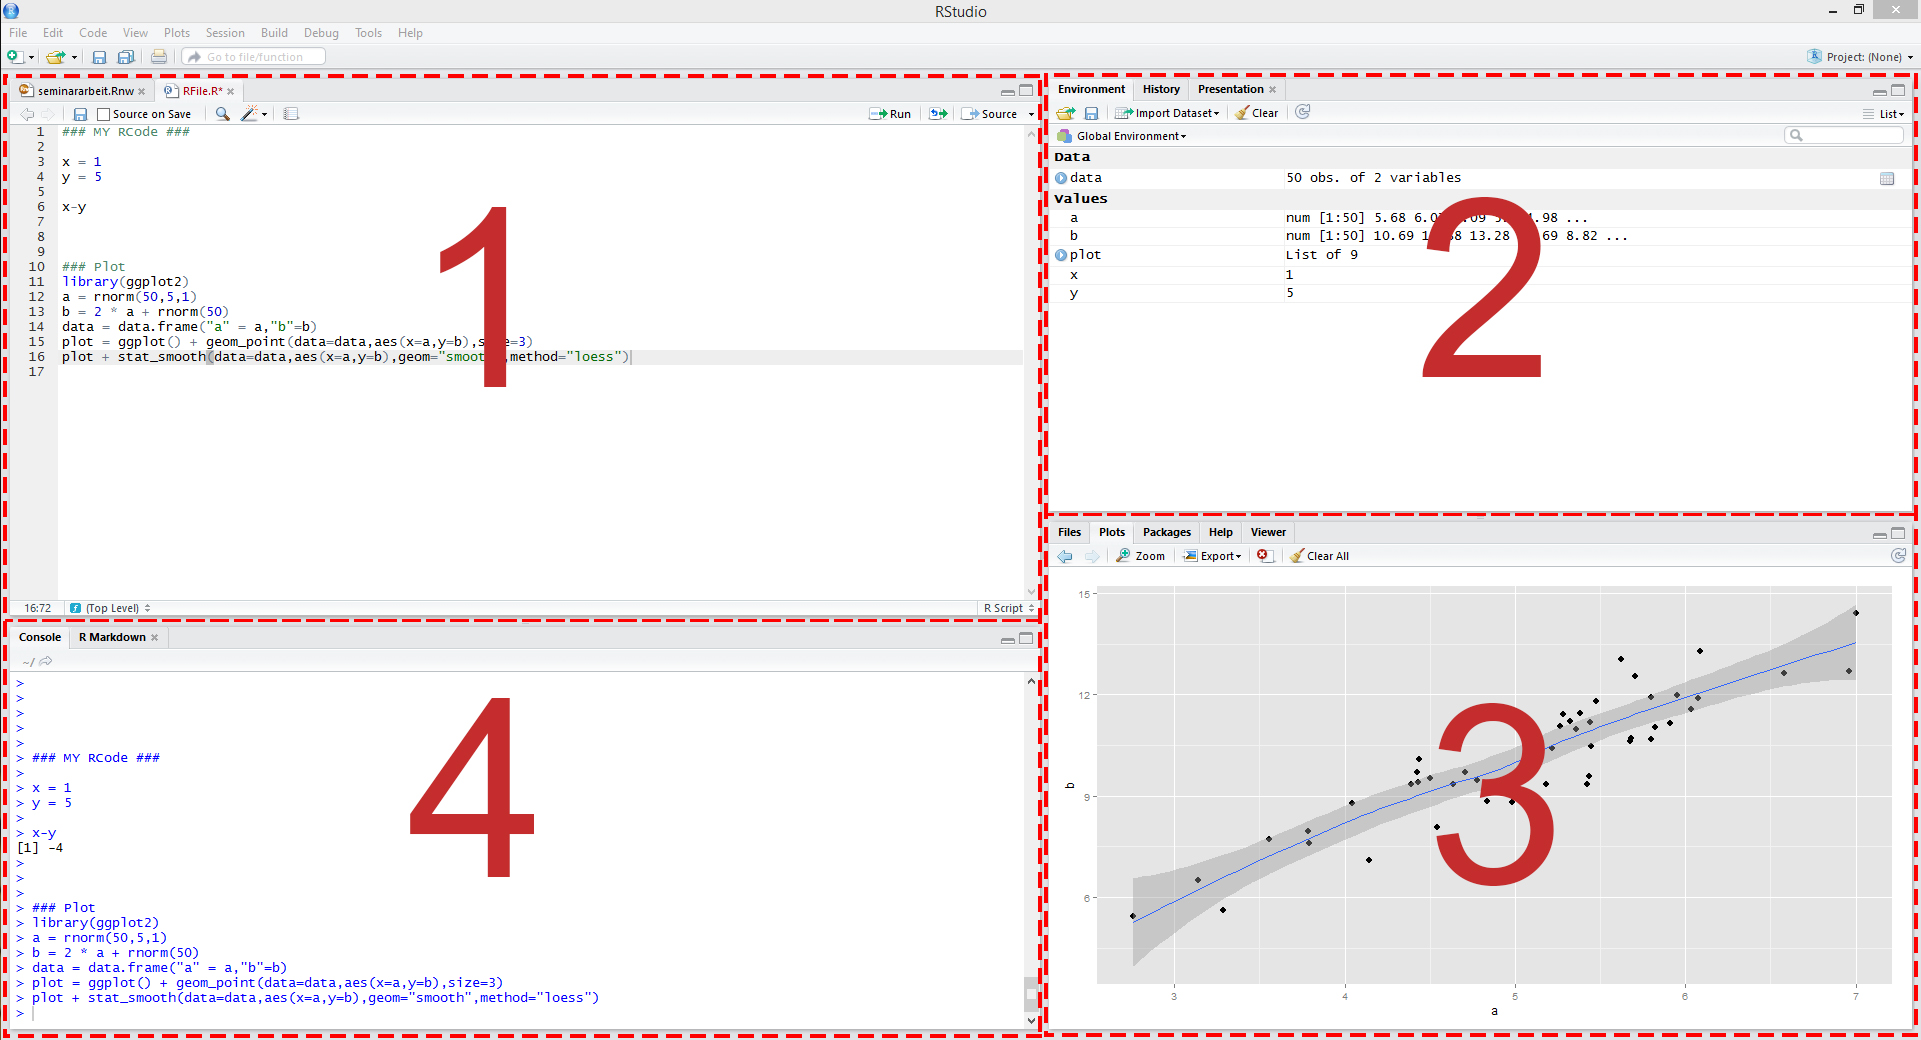
\includegraphics[width=1\linewidth]{images/rstudio} 

}

\caption{RStudio: the four panes}\label{fig:unnamed-chunk-7}
\end{figure}

\subsubsection*{\texorpdfstring{\texttt{R}
Basics}{ Basics}}\label{basics}
\addcontentsline{toc}{subsubsection}{\texttt{R} Basics}

As mentioned before, this book is not intended to be an introduction to
\texttt{R} but as a guide on how to use its capabilities for
applications commonly encountered in undergraduate econometrics. Those
having basic knowledge in \texttt{R} programming will feel comfortable
starting with Chapter \ref{pt}. This section, however, is meant for
those who have not worked with \texttt{R} or \emph{RStudio} before. If
you at least know how to create objects and call functions, you can skip
it. If you would like to refresh your skills or get a feeling for how to
work with \emph{RStudio}, keep reading.

First of all start \emph{RStudio} and open a new \texttt{R} script by
selecting \emph{File}, \emph{New File}, \emph{R Script}. In the editor
pane, type

\begin{Shaded}
\begin{Highlighting}[]
\DecValTok{1} \OperatorTok{+}\StringTok{ }\DecValTok{1}
\end{Highlighting}
\end{Shaded}

and click on the button labeled \emph{Run} in the top right corner of
the editor. By doing so, your line of code is sent to the console and
the result of this operation should be displayed right underneath it. As
you can see, \texttt{R} works just like a calculator. You can do all
arithmetic calculations by using the corresponding operator (\texttt{+},
\texttt{-}, \texttt{*}, \texttt{/} or \texttt{\textasciicircum{}}). If
you are not sure what the last operator does, try it out and check the
results.

\subsubsection*{Vectors}\label{vectors}
\addcontentsline{toc}{subsubsection}{Vectors}

\texttt{R} is of course more sophisticated than that. We can work with
variables or, more generally, objects. Objects are defined by using the
assignment operator \texttt{<-}. To create a variable named \texttt{x}
which contains the value \texttt{10} type \texttt{x\ \textless{}-\ 10}
and click the button \emph{Run} yet again. The new variable should have
appeared in the environment pane on the top right. The console however
did not show any results, because our line of code did not contain any
call that creates output. When you now type \texttt{x} in the console
and hit return, you ask \texttt{R} to show you the value of \texttt{x}
and the corresponding value should be printed in the console.

\texttt{x} is a scalar, a vector of length \(1\). You can easily create
longer vectors by using the function \texttt{c()} (\emph{c} for
``concatenate'' or ``combine''). To create a vector \texttt{y}
containing the numbers \(1\) to \(5\) and print it, do the following.

\begin{Shaded}
\begin{Highlighting}[]
\NormalTok{y <-}\StringTok{ }\KeywordTok{c}\NormalTok{(}\DecValTok{1}\NormalTok{, }\DecValTok{2}\NormalTok{, }\DecValTok{3}\NormalTok{, }\DecValTok{4}\NormalTok{, }\DecValTok{5}\NormalTok{)}
\NormalTok{y}
\end{Highlighting}
\end{Shaded}

\begin{verbatim}
## [1] 1 2 3 4 5
\end{verbatim}

You can also create a vector of letters or words. For now just remember
that characters have to be surrounded by quotes, else they will be
parsed as object names.

\begin{Shaded}
\begin{Highlighting}[]
\NormalTok{hello <-}\StringTok{ }\KeywordTok{c}\NormalTok{(}\StringTok{"Hello"}\NormalTok{, }\StringTok{"World"}\NormalTok{)}
\end{Highlighting}
\end{Shaded}

Here we have created a vector of length 2 containing the words
\texttt{Hello} and \texttt{World}.

Do not forget to save your script! To do so, select \emph{File},
\emph{Save}.

\subsubsection*{Functions}\label{functions}
\addcontentsline{toc}{subsubsection}{Functions}

You have seen the function \texttt{c()} that can be used to combine
objects. In general, all function calls look the same: a function name
is always followed by round parentheses. Sometimes, the parentheses
include arguments.

Here are two simple examples.

\begin{Shaded}
\begin{Highlighting}[]
\CommentTok{# generate the vector `z`}
\NormalTok{z <-}\StringTok{ }\KeywordTok{seq}\NormalTok{(}\DataTypeTok{from =} \DecValTok{1}\NormalTok{, }\DataTypeTok{to =} \DecValTok{5}\NormalTok{, }\DataTypeTok{by =} \DecValTok{1}\NormalTok{)}

\CommentTok{# compute the mean of the enries in `z`}
\KeywordTok{mean}\NormalTok{(}\DataTypeTok{x =}\NormalTok{ z)}
\end{Highlighting}
\end{Shaded}

\begin{verbatim}
## [1] 3
\end{verbatim}

In the first line we use a function called \texttt{seq()} to create the
exact same vector as we did in the previous section, calling it
\texttt{z}. The function takes on the arguments \texttt{from},
\texttt{to} and \texttt{by} which should be self-explanatory. The
function \texttt{mean()} computes the arithmetic mean of its argument
\texttt{x}. Since we pass the vector \texttt{z} as the argument
\texttt{x}, the result is \texttt{3}!

If you are not sure which arguments a function expects, you may consult
the function's documentation. Let's say we are not sure how the
arguments required for \texttt{seq()} work. We then type \texttt{?seq}
in the console. By hitting return the documentation page for that
function pops up in the lower right pane of \emph{RStudio}. In there,
the section \emph{Arguments} holds the information we seek. On the
bottom of almost every help page you find examples on how to use the
corresponding functions. This is very helpful for beginners and we
recommend to look out for those.

Of course, all of the commands presented above also work in interactive
widgets throughout the book. You may try them below.

\chapter{Probability Theory}\label{pt}

This chapter reviews some basic concepts of probability theory and
demonstrates how they can be applied in \texttt{R}.

Most of the statistical functionalities in \texttt{R}'s standard version
are collected in the \texttt{stats} package. It provides simple
functions which compute descriptive measures and facilitate computations
involving a variety of probability distributions. It also contains more
sophisticated routines that, e.g., enable the user to estimate a large
number of models based on the same data or help to conduct extensive
simulation studies. \texttt{stats} is part of the base distribution of
\texttt{R}, meaning that it is installed by default so there is no need
to run \texttt{install.packages("stats")} or \texttt{library("stats")}.
Simply execute \texttt{library(help\ =\ "stats")} in the console to view
the documentation and a complete list of all functions gathered in
\texttt{stats}. For most packages a documentation that can be viewed
within \emph{RStudio} is available. Documentations can be invoked using
the \texttt{?} operator, e.g., upon execution of \texttt{?stats} the
documentation of the \texttt{stats} package is shown in the help tab of
the bottom-right pane.

In what follows, our focus is on (some of) the probability distributions
that are handled by \texttt{R} and show how to use the relevant
functions to solve simple problems. Thereby, we refresh some core
concepts of probability theory. Among other things, you will learn how
to draw random numbers, how to compute densities, probabilities,
quantiles and alike. As we shall see, it is very convenient to rely on
these routines.

\section{Random Variables and Probability
Distributions}\label{random-variables-and-probability-distributions}

Let us briefly review some basic concepts of probability theory.

\begin{itemize}
\tightlist
\item
  The mutually exclusive results of a random process are called the
  \emph{outcomes}. `Mutually exclusive' means that only one of the
  possible outcomes can be observed.
\item
  We refer to the \emph{probability} of an outcome as the proportion
  that the outcome occurs in the long run, that is, if the experiment is
  repeated very often.
\item
  The set of all possible outcomes of a random variable is called the
  \emph{sample space}.
\item
  An \emph{event} is a subset of the sample space and consists of one or
  more outcomes.
\end{itemize}

These ideas are unified in the concept of a \emph{random variable} which
is a numerical summary of random outcomes. Random variables can be
\emph{discrete} or \emph{continuous}.

\begin{itemize}
\tightlist
\item
  Discrete random variables have discrete outcomes, e.g., \(0\) and
  \(1\).
\item
  A continuous random variable may take on a continuum of possible
  values.
\end{itemize}

\subsection*{Probability Distributions of Discrete Random
Variables}\label{probability-distributions-of-discrete-random-variables}
\addcontentsline{toc}{subsection}{Probability Distributions of Discrete
Random Variables}

A typical example for a discrete random variable \(D\) is the result of
a dice roll: in terms of a random experiment this is nothing but
randomly selecting a sample of size \(1\) from a set of numbers which
are mutually exclusive outcomes. Here, the sample space is
\(\{1,2,3,4,5,6\}\) and we can think of many different events, e.g.,
`the observed outcome lies between \(2\) and \(5\)'.

A basic function to draw random samples from a specified set of elements
is the the function \texttt{sample()}, see \texttt{?sample}. We can use
it to simulate the random outcome of a dice roll. Let's roll the dice!

\begin{Shaded}
\begin{Highlighting}[]
\KeywordTok{sample}\NormalTok{(}\DecValTok{1}\OperatorTok{:}\DecValTok{6}\NormalTok{, }\DecValTok{1}\NormalTok{) }
\end{Highlighting}
\end{Shaded}

\begin{verbatim}
## [1] 6
\end{verbatim}

The probability distribution of a discrete random variable is the list
of all possible values of the variable and their probabilities which sum
to \(1\). The cumulative probability distribution function gives the
probability that the random variable is less than or equal to a
particular value.

For the dice roll, the probability distribution and the cumulative
probability distribution are summarized in Table \ref{tab:pdist}.

\begin{table}

\caption{\label{tab:pdist}PDF and CDF of a Dice Roll}
\centering
\begin{tabular}[t]{l|l|l|l|l|l|l}
\hline
Outcome & 1 & 2 & 3 & 4 & 5 & 6\\
\hline
Probability & 1/6 & 1/6 & 1/6 & 1/6 & 1/6 & 1/6\\
\hline
Cumulative Probability & 1/6 & 2/6 & 3/6 & 4/6 & 5/6 & 1\\
\hline
\end{tabular}
\end{table}

We can easily plot both functions using \texttt{R}. Since the
probability equals \(1/6\) for each outcome, we set up the vector
\texttt{probability} by using the function \texttt{rep()} which
replicates a given value a specified number of times.

\begin{Shaded}
\begin{Highlighting}[]
\CommentTok{# generate the vector of probabilities }
\NormalTok{probability <-}\StringTok{ }\KeywordTok{rep}\NormalTok{(}\DecValTok{1}\OperatorTok{/}\DecValTok{6}\NormalTok{, }\DecValTok{6}\NormalTok{) }

\CommentTok{# plot the probabilites }
\KeywordTok{plot}\NormalTok{(probability, }
     \DataTypeTok{main =} \StringTok{"Probability Distribution"}\NormalTok{,}
     \DataTypeTok{xlab =} \StringTok{"outcomes"}\NormalTok{) }
\end{Highlighting}
\end{Shaded}

\begin{center}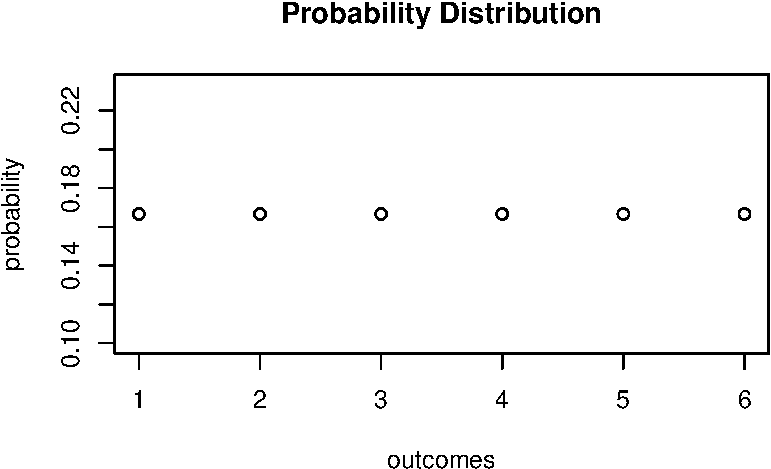
\includegraphics{ITER_files/figure-latex/unnamed-chunk-14-1} \end{center}

For the cumulative probability distribution we need the cumulative
probabilities, i.e., we need the cumulative sums of the vector
\texttt{probability}. These sums can be computed using
\texttt{cumsum()}.

\begin{Shaded}
\begin{Highlighting}[]
\CommentTok{# generate the vector of cumulative probabilities }
\NormalTok{cum_probability <-}\StringTok{ }\KeywordTok{cumsum}\NormalTok{(probability) }

\CommentTok{# plot the probabilites }
\KeywordTok{plot}\NormalTok{(cum_probability, }
     \DataTypeTok{xlab =} \StringTok{"outcomes"}\NormalTok{, }
     \DataTypeTok{main =} \StringTok{"Cumulative Probability Distribution"}\NormalTok{) }
\end{Highlighting}
\end{Shaded}

\begin{center}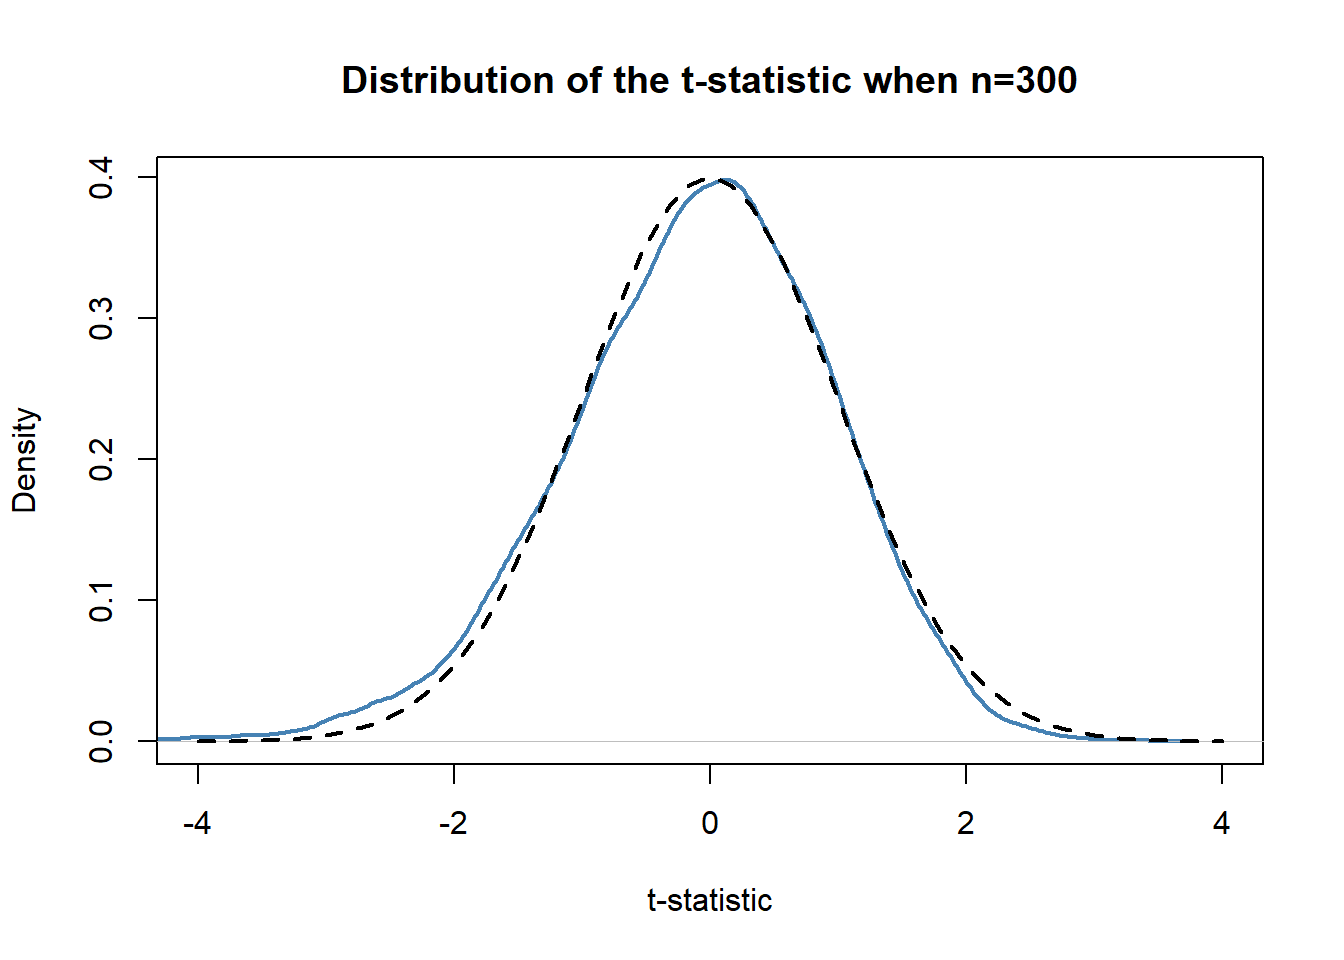
\includegraphics{ITER_files/figure-latex/unnamed-chunk-15-1} \end{center}

\subsection*{Bernoulli Trials}\label{bernoulli-trials}
\addcontentsline{toc}{subsection}{Bernoulli Trials}

The set of elements from which \texttt{sample()} draws outcomes does not
have to consist of numbers only. We might as well simulate coin tossing
with outcomes \(H\) (heads) and \(T\) (tails).

\begin{Shaded}
\begin{Highlighting}[]
\KeywordTok{sample}\NormalTok{(}\KeywordTok{c}\NormalTok{(}\StringTok{"H"}\NormalTok{, }\StringTok{"T"}\NormalTok{), }\DecValTok{1}\NormalTok{) }
\end{Highlighting}
\end{Shaded}

\begin{verbatim}
## [1] "T"
\end{verbatim}

The result of a single coin toss is a \emph{Bernoulli} distributed
random variable, i.e., a variable with two possible distinct outcomes.

Imagine you are about to toss a coin \(10\) times in a row and wonder
how likely it is to end up with a \(5\) times heads. This is a typical
example of what we call a \emph{Bernoulli experiment} as it consists of
\(n=10\) Bernoulli trials that are independent of each other and we are
interested in the likelihood of observing \(k=5\) successes \(H\) that
occur with probability \(p=0.5\) (assuming a fair coin) in each trial.
Note that the order of the outcomes does not matter here.

It is a \href{https://en.wikipedia.org/wiki/Binomial_distribution}{well
known result} that the number of successes \(k\) in a Bernoulli
experiment follows a binomial distribution. We denote this as

\[k \sim B(n,p).\]

The probability of observing \(k\) successes in the experiment
\(B(n,p)\) is given by

\[f(k)=P(k)=\begin{pmatrix}n\\ k \end{pmatrix} \cdot p^k \cdot
(1-p)^{n-k}=\frac{n!}{k!(n-k)!} \cdot p^k \cdot (1-p)^{n-k}\]

with \(\begin{pmatrix}n\\ k \end{pmatrix}\) the binomial coefficient.

In \texttt{R}, we can solve the problem stated above by means of the
function \texttt{dbinom()} which calculates the probability of the
binomial distribution given the parameters \texttt{x}, \texttt{size},
and \texttt{prob}, see \texttt{?binom}.

\begin{Shaded}
\begin{Highlighting}[]
\KeywordTok{dbinom}\NormalTok{(}\DataTypeTok{x =} \DecValTok{5}\NormalTok{,}
       \DataTypeTok{size =} \DecValTok{10}\NormalTok{,}
       \DataTypeTok{prob =} \FloatTok{0.5}\NormalTok{) }
\end{Highlighting}
\end{Shaded}

\begin{verbatim}
## [1] 0.2460938
\end{verbatim}

We conclude that the probability of observing Head \(k=5\) times when
tossing the coin \(n=10\) times is about \(24.6\%\).

Now assume we are interested in \(P(4 \leq k \leq 7)\), i.e., the
probability of observing \(4\), \(5\), \(6\) or \(7\) successes for
\(B(10,0.5)\). This may be computed by providing a vector as the
argument \texttt{x} in our call of \texttt{dbinom()} and summing up
using \texttt{sum()}.

\begin{Shaded}
\begin{Highlighting}[]
\CommentTok{# compute P(4 <= k <= 7) using 'dbinom()'}
\KeywordTok{sum}\NormalTok{(}\KeywordTok{dbinom}\NormalTok{(}\DataTypeTok{x =} \DecValTok{4}\OperatorTok{:}\DecValTok{7}\NormalTok{, }
         \DataTypeTok{size =} \DecValTok{10}\NormalTok{, }
         \DataTypeTok{prob =} \FloatTok{0.5}\NormalTok{))}
\end{Highlighting}
\end{Shaded}

\begin{verbatim}
## [1] 0.7734375
\end{verbatim}

An alternative approach is to use \texttt{pbinom()}, the distribution
function of the binomial distribution to compute
\[P(4 \leq k \leq 7) = P(k \leq 7) - P(k\leq3 ).\]

\begin{Shaded}
\begin{Highlighting}[]
\CommentTok{# compute P(4 <= k <= 7) using 'pbinom()'}
\KeywordTok{pbinom}\NormalTok{(}\DataTypeTok{size =} \DecValTok{10}\NormalTok{, }\DataTypeTok{prob =} \FloatTok{0.5}\NormalTok{, }\DataTypeTok{q =} \DecValTok{7}\NormalTok{) }\OperatorTok{-}\StringTok{ }\KeywordTok{pbinom}\NormalTok{(}\DataTypeTok{size =} \DecValTok{10}\NormalTok{, }\DataTypeTok{prob =} \FloatTok{0.5}\NormalTok{, }\DataTypeTok{q =} \DecValTok{3}\NormalTok{) }
\end{Highlighting}
\end{Shaded}

\begin{verbatim}
## [1] 0.7734375
\end{verbatim}

The probability distribution of a discrete random variable is nothing
but a list of all possible outcomes that can occur and their respective
probabilities. In the coin tossing example we have \(11\) possible
outcomes for \(k\).

\begin{Shaded}
\begin{Highlighting}[]
\CommentTok{# set up vector of possible outcomes}
\NormalTok{k <-}\StringTok{ }\DecValTok{0}\OperatorTok{:}\DecValTok{10}
\end{Highlighting}
\end{Shaded}

To visualize the probability distribution function of \(k\) we may
therefore do the following:

\begin{Shaded}
\begin{Highlighting}[]
\CommentTok{# assign the probabilities}
\NormalTok{probability <-}\StringTok{ }\KeywordTok{dbinom}\NormalTok{(}\DataTypeTok{x =}\NormalTok{ k,}
                      \DataTypeTok{size =} \DecValTok{10}\NormalTok{, }
                      \DataTypeTok{prob =} \FloatTok{0.5}\NormalTok{)}

\CommentTok{# plot the outcomes against their probabilities}
\KeywordTok{plot}\NormalTok{(}\DataTypeTok{x =}\NormalTok{ k, }
     \DataTypeTok{y =}\NormalTok{ probability,}
     \DataTypeTok{main =} \StringTok{"Probability Distribution Function"}\NormalTok{) }
\end{Highlighting}
\end{Shaded}

\begin{center}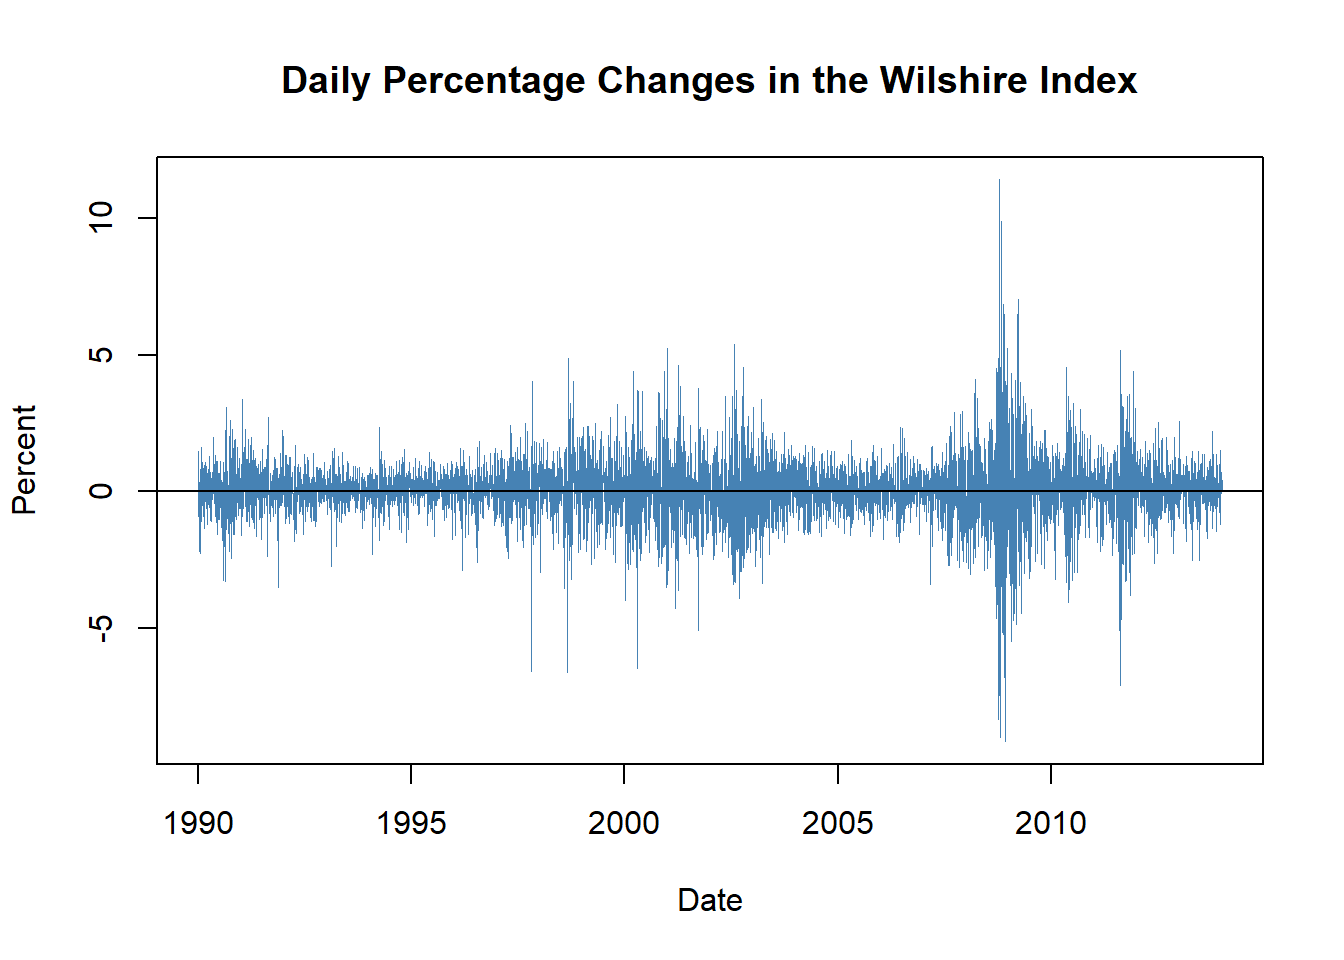
\includegraphics{ITER_files/figure-latex/unnamed-chunk-21-1} \end{center}

In a similar fashion we may plot the cumulative distribution function of
\(k\) by executing the following code chunk:

\begin{Shaded}
\begin{Highlighting}[]
\CommentTok{# compute cumulative probabilities}
\NormalTok{prob <-}\StringTok{ }\KeywordTok{dbinom}\NormalTok{(}\DataTypeTok{x =} \DecValTok{0}\OperatorTok{:}\DecValTok{10}\NormalTok{, }
               \DataTypeTok{size =} \DecValTok{10}\NormalTok{, }
               \DataTypeTok{prob =} \FloatTok{0.5}\NormalTok{)}

\CommentTok{# plot the cumulative probabilities}
\KeywordTok{plot}\NormalTok{(}\DataTypeTok{x =}\NormalTok{ k, }
     \DataTypeTok{y =}\NormalTok{ prob,}
     \DataTypeTok{main =} \StringTok{"Cumulative Distribution Function"}\NormalTok{) }
\end{Highlighting}
\end{Shaded}

\begin{center}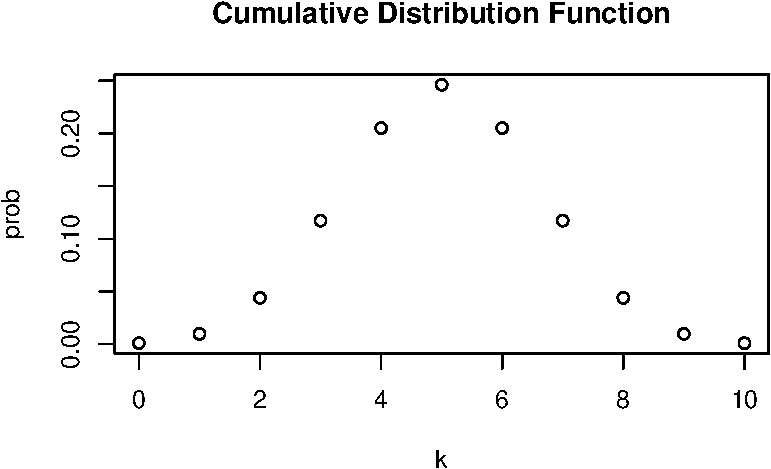
\includegraphics{ITER_files/figure-latex/unnamed-chunk-22-1} \end{center}

\subsection*{Expected Value, Mean and
Variance}\label{expected-value-mean-and-variance}
\addcontentsline{toc}{subsection}{Expected Value, Mean and Variance}

The expected value of a random variable is, loosely, the long-run
average value of its outcomes when the number of repeated trials is
large. For a discrete random variable, the expected value is computed as
a weighted average of its possible outcomes whereby the weights are the
related probabilities. This is formalized in Key Concept 2.1.

\begin{keyconcepts}[Expected Value and the Mean]{2.1}
Suppose the random variable $Y$
takes on $k$ possible values, $y_1, \dots, y_k$, where $y_1$ denotes the first
value, $y_2$ denotes the second value, and so forth, and that the probability
that $Y$ takes on $y_1$ is $p_1$, the probability that $Y$ takes on $y_2$ is
$p_2$ and so forth. The expected value of $Y$, $E(Y)$ is defined as

$$ E(Y) = y_1 p_1 + y_2 p_2 + \cdots + y_k p_k = \sum_{i=1}^k y_i p_i $$

where the notation $\sum_{i=1}^k y_i p_i$ means \"the sum of $y_i$ $p_i$ for $i$
running from $1$ to $k$\". The expected value of $Y$ is also called the mean of $Y$
or the expectation of $Y$ and is denoted by $\mu_Y$.
\end{keyconcepts}

In the dice example, the random variable, \(D\) say, takes on \(6\)
possible values \(d_1 = 1, d_2 = 2, \dots, d_6 = 6\). Assuming a fair
dice, each of the \(6\) outcomes occurs with a probability of \(1/6\).
It is therefore easy to calculate the exact value of \(E(D)\) by hand:

\[ E(D) = 1/6 \sum_{i=1}^6 d_i = 3.5 \]

\(E(D)\) is simply the average of the natural numbers from \(1\) to
\(6\) since all wights \(p_i\) are \(1/6\). This can be easily
calculated using the function \texttt{mean()} which computes the
arithmetic mean of a numeric vector.

\begin{Shaded}
\begin{Highlighting}[]
\CommentTok{# compute mean of natural numbers from 1 to 6}
\KeywordTok{mean}\NormalTok{(}\DecValTok{1}\OperatorTok{:}\DecValTok{6}\NormalTok{)}
\end{Highlighting}
\end{Shaded}

\begin{verbatim}
## [1] 3.5
\end{verbatim}

An example of sampling with replacement is rolling a dice three times in
a row.

\begin{Shaded}
\begin{Highlighting}[]
\CommentTok{# set seed for reproducibility}
\KeywordTok{set.seed}\NormalTok{(}\DecValTok{1}\NormalTok{)}

\CommentTok{# rolling a dice three times in a row}
\KeywordTok{sample}\NormalTok{(}\DecValTok{1}\OperatorTok{:}\DecValTok{6}\NormalTok{, }\DecValTok{3}\NormalTok{, }\DataTypeTok{replace =}\NormalTok{ T)}
\end{Highlighting}
\end{Shaded}

\begin{verbatim}
## [1] 2 3 4
\end{verbatim}

Of course we could also consider a much bigger number of trials,
\(10000\) say. Doing so, it would be pointless to simply print the
results to the console: by default \texttt{R} displays up to \(1000\)
entries of large vectors and omits the remainder (give it a try).
Eyeballing the numbers does not reveal much. Instead, let us calculate
the sample average of the outcomes using \texttt{mean()} and see if the
result comes close to the expected value \(E(D)=3.5\).

\begin{Shaded}
\begin{Highlighting}[]
\CommentTok{# set seed for reproducibility}
\KeywordTok{set.seed}\NormalTok{(}\DecValTok{1}\NormalTok{)}

\CommentTok{# compute the sample mean of 10000 dice rolls}
\KeywordTok{mean}\NormalTok{(}\KeywordTok{sample}\NormalTok{(}\DecValTok{1}\OperatorTok{:}\DecValTok{6}\NormalTok{, }
           \DecValTok{10000}\NormalTok{, }
           \DataTypeTok{replace =}\NormalTok{ T))}
\end{Highlighting}
\end{Shaded}

\begin{verbatim}
## [1] 3.5039
\end{verbatim}

We find the sample mean to be fairly close to the expected value. This
result will be discussed in Chapter \ref{RSATDOSA} in more detail.

Other frequently encountered measures are the variance and the standard
deviation. Both are measures of the \emph{dispersion} of a random
variable.

\begin{keyconcepts}[Variance and Standard Deviation]{2.2}
The variance of the discrete \textit{random variable} $Y$, denoted $\sigma^2_Y$, is
$$ \sigma^2_Y = \text{Var}(Y) = E\left[(Y-\mu_Y)^2\right] = \sum_{i=1}^k (y_i - \mu_Y)^2 p_i $$
The standard deviation of $Y$ is $\sigma_Y$, the square root of the variance. The units of the standard deviation are the same as the units of $Y$.
\end{keyconcepts}

The variance as defined in Key Concept 2.2, being a population quantity,
\emph{is not} implemented as a function in R. Instead we have the
function \texttt{var()} which computes the \emph{sample variance}

\[ s^2_Y = \frac{1}{n-1} \sum_{i=1}^n (y_i - \overline{y})^2. \]

Remember that \(s^2_Y\) is different from the so called \emph{population
variance} of a discrete random variable \(Y\),

\[ \text{Var}(Y) = \frac{1}{N} \sum_{i=1}^N (y_i - \mu_Y)^2. \]

since it measures how the data is dispersed around the sample average
\(\overline{y}\) instead of the population mean \(\mu_Y\). This becomes
clear when we look at our dice rolling example. For \(D\) we have

\[ \text{Var}(D) = 1/6 \sum_{i=1}^6 (d_i - 3.5)^2 = 2.92  \] which is
obviously different from the result of \(s^2\) as computed by
\texttt{var()}.

\begin{Shaded}
\begin{Highlighting}[]
\KeywordTok{var}\NormalTok{(}\DecValTok{1}\OperatorTok{:}\DecValTok{6}\NormalTok{)}
\end{Highlighting}
\end{Shaded}

\begin{verbatim}
## [1] 3.5
\end{verbatim}

The sample variance as computed by \texttt{var()} is an \emph{estimator}
of the population variance. You may check this using the widget below.

\subsection*{Probability Distributions of Continuous Random
Variables}\label{probability-distributions-of-continuous-random-variables}
\addcontentsline{toc}{subsection}{Probability Distributions of
Continuous Random Variables}

Since a continuous random variable takes on a continuum of possible
values, we cannot use the concept of a probability distribution as used
for discrete random variables. Instead, the probability distribution of
a continuous random variable is summarized by its \emph{probability
density function} (PDF).

The cumulative probability distribution function (CDF) for a continuous
random variable is defined just as in the discrete case. Hence, the
cumulative probability distribution of a continuous random variables
states the probability that the random variable is less than or equal to
a particular value.

For completeness, we present revisions of Key Concepts 2.1 and 2.2 for
the continuous case.

\begin{keyconcepts}[Probabilities\comma Expected Value and Variance of a Continuous Random Variable]{2.3}
Let $f_Y(y)$ denote the probability density function of $Y$. The Probability that $Y$ falls between $a$ and $b$ where $a < b$ is 
$$ P(a \leq Y \leq b) = \int_a^b f_Y(y) \mathrm{d}y. $$
We further have that $P(-\infty \leq Y \leq \infty) = 1$ and therefore $\int_{-\infty}^{\infty} f_Y(y) \mathrm{d}y = 1$.

As for the discrete case, the expected value of $Y$ is the probability weighted average of its values. Due to continuity, we use integrals instead of sums. The expected value of $Y$ is defined as

$$ E(Y) =  \mu_Y = \int y f_Y(y) \mathrm{d}y. $$

The variance is the expected value of $(Y - \mu_Y)^2$. We thus have

$$\text{Var}(Y) =  \sigma_Y^2 = \int (y - \mu_Y)^2 f_Y(y) \mathrm{d}y.$$
\end{keyconcepts}

Let us discuss an example:

Consider the continuous random variable \(X\) with probability density
function

\[ f_X(x) = \frac{3}{x^4}, x>1. \]

\begin{itemize}
\tightlist
\item
  We can show analytically that the integral of \(f_X(x)\) over the real
  line equals \(1\).
\end{itemize}

\begin{align}
 \int f_X(x) \mathrm{d}x =&  \int_{1}^{\infty} \frac{3}{x^4} \mathrm{d}x \\
  =& \lim_{t \rightarrow \infty} \int_{1}^{t} \frac{3}{x^4} \mathrm{d}x \\
  =& \lim_{t \rightarrow \infty}  -x^{-3} \rvert_{x=1}^t \\
  =& -\left(\lim_{t \rightarrow \infty}\frac{1}{t^3} - 1\right) \\
  =& 1
\end{align}

\begin{itemize}
\tightlist
\item
  The expectation of \(X\) can be computed as follows:
\end{itemize}

\begin{align}
 E(X) = \int x \cdot f_X(x) \mathrm{d}x =&  \int_{1}^{\infty} x \cdot \frac{3}{x^4} \mathrm{d}x \\
  =& - \frac{3}{2} x^{-2} \rvert_{x=1}^{\infty} \\
  =& -\frac{3}{2} \left( \lim_{t \rightarrow \infty} \frac{1}{t^2} - 1 \right) \\
  =& \frac{3}{2}
\end{align}

\begin{itemize}
\tightlist
\item
  Note that the variance of \(X\) can be expressed as
  \(\text{Var}(X) = E(X^2) - E(X)^2\). Since \(E(X)\) has been computed
  in the previous step, we seek \(E(X^2)\):
\end{itemize}

\begin{align}
 E(X^2)= \int x^2 \cdot f_X(x) \mathrm{d}x =&  \int_{1}^{\infty} x^2 \cdot \frac{3}{x^4} \mathrm{d}x \\
  =& -3 x^{-1} \rvert_{x=1}^{\infty} \\
  =& -3 \left( \lim_{t \rightarrow \infty} \frac{1}{t} - 1 \right) \\
  =& 3
\end{align}

So we have shown that the area under the curve equals one, that the
expectation is \(E(X)=\frac{3}{2} \ \) and we found the variance to be
\(\text{Var}(X) = \frac{3}{4}\). However, this was tedious and, as we
shall see, an analytic approach is not applicable for some probability
density functions, e.g., if integrals have no closed form solutions.

Luckily, \texttt{R} also enables us to easily find the results derived
above. The tool we use for this is the function \texttt{integrate()}.
First, we have to define the functions we want to calculate integrals
for as \texttt{R} functions, i.e., the PDF \(f_X(x)\) as well as the
expressions \(x\cdot f_X(x)\) and \(x^2\cdot f_X(x)\).

\begin{Shaded}
\begin{Highlighting}[]
\CommentTok{# define functions}
\NormalTok{f <-}\StringTok{ }\ControlFlowTok{function}\NormalTok{(x) }\DecValTok{3} \OperatorTok{/}\StringTok{ }\NormalTok{x}\OperatorTok{^}\DecValTok{4}
\NormalTok{g <-}\StringTok{ }\ControlFlowTok{function}\NormalTok{(x) x }\OperatorTok{*}\StringTok{ }\KeywordTok{f}\NormalTok{(x)}
\NormalTok{h <-}\StringTok{ }\ControlFlowTok{function}\NormalTok{(x) x}\OperatorTok{^}\DecValTok{2} \OperatorTok{*}\StringTok{ }\KeywordTok{f}\NormalTok{(x)}
\end{Highlighting}
\end{Shaded}

Next, we use \texttt{integrate()} and set lower and upper limits of
integration to \(1\) and \(\infty\) using arguments \texttt{lower} and
\texttt{upper}. By default, \texttt{integrate()} prints the result along
with an estimate of the approximation error to the console. However, the
outcome is not a numeric value one can readily do further calculation
with. In order to get only a numeric value of the integral, we need to
use the \texttt{\textbackslash{}\$} operator in conjunction with
\texttt{value}. The \texttt{\textbackslash{}\$} operator is used to
extract elements by name from an object of type \texttt{list}.

\begin{Shaded}
\begin{Highlighting}[]
\CommentTok{# compute area under the density curve}
\NormalTok{area <-}\StringTok{ }\KeywordTok{integrate}\NormalTok{(f, }
                 \DataTypeTok{lower =} \DecValTok{1}\NormalTok{, }
                 \DataTypeTok{upper =} \OtherTok{Inf}\NormalTok{)}\OperatorTok{$}\NormalTok{value}
\NormalTok{area }
\end{Highlighting}
\end{Shaded}

\begin{verbatim}
## [1] 1
\end{verbatim}

\begin{Shaded}
\begin{Highlighting}[]
\CommentTok{# compute E(X)}
\NormalTok{EX <-}\StringTok{ }\KeywordTok{integrate}\NormalTok{(g,}
                \DataTypeTok{lower =} \DecValTok{1}\NormalTok{,}
                \DataTypeTok{upper =} \OtherTok{Inf}\NormalTok{)}\OperatorTok{$}\NormalTok{value}
\NormalTok{EX}
\end{Highlighting}
\end{Shaded}

\begin{verbatim}
## [1] 1.5
\end{verbatim}

\begin{Shaded}
\begin{Highlighting}[]
\CommentTok{# compute Var(X)}
\NormalTok{VarX <-}\StringTok{ }\KeywordTok{integrate}\NormalTok{(h,}
                  \DataTypeTok{lower =} \DecValTok{1}\NormalTok{,}
                  \DataTypeTok{upper =} \OtherTok{Inf}\NormalTok{)}\OperatorTok{$}\NormalTok{value }\OperatorTok{-}\StringTok{ }\NormalTok{EX}\OperatorTok{^}\DecValTok{2} 
\NormalTok{VarX}
\end{Highlighting}
\end{Shaded}

\begin{verbatim}
## [1] 0.75
\end{verbatim}

Although there is a wide variety of distributions, the ones most often
encountered in econometrics are the normal, chi-squared, Student \(t\)
and \(F\) distributions. Therefore we will discuss some core \texttt{R}
functions that allow to do calculations involving densities,
probabilities and quantiles of these distributions.

Every probability distribution that \texttt{R} handles has four basic
functions whose names consist of a prefix followed by a root name. As an
example, take the normal distribution. The root name of all four
functions associated with the normal distribution is \texttt{norm}. The
four prefixes are

\begin{itemize}
\tightlist
\item
  \texttt{d} for ``density'' - probability function / probability
  density function
\item
  \texttt{p} for ``probability'' - cumulative distribution function
\item
  \texttt{q} for ``quantile'' - quantile function (inverse cumulative
  distribution function)
\item
  \texttt{r} for ``random'' - random number generator
\end{itemize}

Thus, for the normal distribution we have the \texttt{R} functions
\texttt{dnorm()}, \texttt{pnorm()}, \texttt{qnorm()} and
\texttt{rnorm()}.

\subsection*{The Normal Distribution}\label{the-normal-distribution}
\addcontentsline{toc}{subsection}{The Normal Distribution}

The probably most important probability distribution considered here is
the normal distribution. This is not least due to the special role of
the standard normal distribution and the Central Limit Theorem which is
to be treated shortly. Normal distributions are symmetric and
bell-shaped. A normal distribution is characterized by its mean \(\mu\)
and its standard deviation \(\sigma\), concisely expressed by
\(\mathcal{N}(\mu,\sigma^2)\). The normal distribution has the PDF

\begin{align}
f(x) = \frac{1}{\sqrt{2 \pi} \sigma} \exp{-(x - \mu)^2/(2 \sigma^2)}.
\end{align}

For the standard normal distribution we have \(\mu=0\) and \(\sigma=1\).
Standard normal variates are often denoted by \(Z\). Usually, the
standard normal PDF is denoted by \(\phi\) and the standard normal CDF
is denoted by \(\Phi\). Hence,
\[ \phi(c) = \Phi'(c) \ \ , \ \ \Phi(c) = P(Z \leq c) \ \ , \ \ Z \sim \mathcal{N}(0,1).\]
In \texttt{R}, we can conveniently obtain densities of normal
distributions using the function \texttt{dnorm()}. Let us draw a plot of
the standard normal density function using \texttt{curve()} in
conjunction with \texttt{dnorm()}.

\begin{Shaded}
\begin{Highlighting}[]
\CommentTok{# draw a plot of the N(0,1) PDF}
\KeywordTok{curve}\NormalTok{(}\KeywordTok{dnorm}\NormalTok{(x),}
      \DataTypeTok{xlim =} \KeywordTok{c}\NormalTok{(}\OperatorTok{-}\FloatTok{3.5}\NormalTok{, }\FloatTok{3.5}\NormalTok{),}
      \DataTypeTok{ylab =} \StringTok{"Density"}\NormalTok{, }
      \DataTypeTok{main =} \StringTok{"Standard Normal Density Function"}\NormalTok{) }
\end{Highlighting}
\end{Shaded}

\begin{center}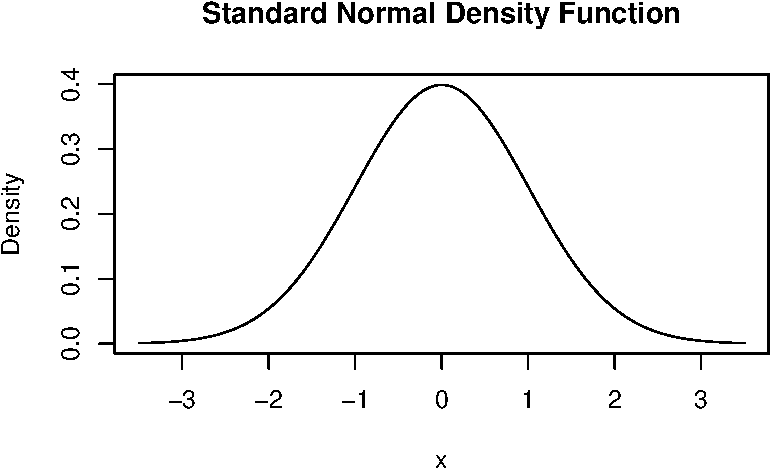
\includegraphics{ITER_files/figure-latex/unnamed-chunk-36-1} \end{center}

We can obtain the density at different positions by passing a vector to
\texttt{dnorm()}.

\begin{Shaded}
\begin{Highlighting}[]
\CommentTok{# compute denstiy at x=-1.96, x=0 and x=1.96}
\KeywordTok{dnorm}\NormalTok{(}\DataTypeTok{x =} \KeywordTok{c}\NormalTok{(}\OperatorTok{-}\FloatTok{1.96}\NormalTok{, }\DecValTok{0}\NormalTok{, }\FloatTok{1.96}\NormalTok{))}
\end{Highlighting}
\end{Shaded}

\begin{verbatim}
## [1] 0.05844094 0.39894228 0.05844094
\end{verbatim}

Similar to the PDF, we can plot the standard normal CDF using
\texttt{curve()}. We could use \texttt{dnorm()} for this but it is much
more convenient to rely on \texttt{pnorm()}.

\begin{Shaded}
\begin{Highlighting}[]
\CommentTok{# plot the standard normal CDF}
\KeywordTok{curve}\NormalTok{(}\KeywordTok{pnorm}\NormalTok{(x), }
      \DataTypeTok{xlim =} \KeywordTok{c}\NormalTok{(}\OperatorTok{-}\FloatTok{3.5}\NormalTok{, }\FloatTok{3.5}\NormalTok{), }
      \DataTypeTok{ylab =} \StringTok{"Density"}\NormalTok{, }
      \DataTypeTok{main =} \StringTok{"Standard Normal Cumulative Distribution Function"}\NormalTok{)}
\end{Highlighting}
\end{Shaded}

\begin{center}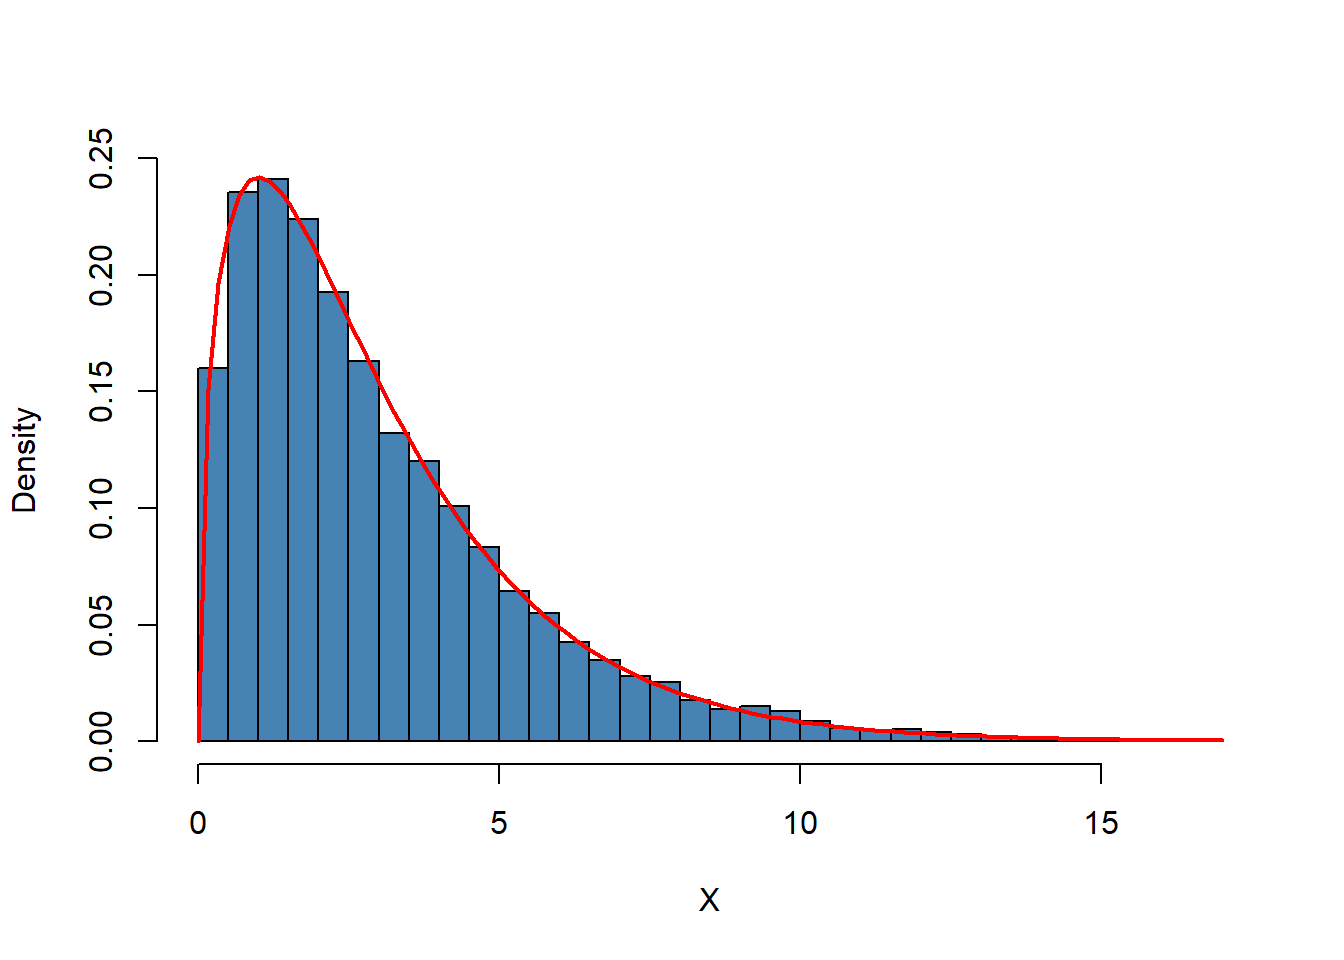
\includegraphics{ITER_files/figure-latex/unnamed-chunk-38-1} \end{center}

We can also use \texttt{R} to calculate the probability of events
associated with a standard normal variate.

Let us say we are interested in \(P(Z \leq 1.337)\). For some continuous
random variable \(Z\) on \([-\infty,\infty]\) with density \(g(x)\) we
would have to determine \(G(x)\), the anti-derivative of \(g(x)\) so
that

\[ P(Z \leq 1.337 ) = G(1.337) = \int_{-\infty}^{1.337} g(x) \mathrm{d}x.  \]

If \(Z \sim \mathcal{N}(0,1)\), we have \(g(x)=\phi(x)\). There is no
analytic solution to the integral above. Fortunately, \texttt{R} offers
good approximations. The first approach makes use of the function
\texttt{integrate()} which allows to solve one-dimensional integration
problems using a numerical method. For this, we first define the
function we want to compute the integral of as an \texttt{R} function
\texttt{f}. In our example, \texttt{f} is the standard normal density
function and hence takes a single argument \texttt{x}. Following the
definition of \(\phi(x)\) we define \texttt{f} as

\begin{Shaded}
\begin{Highlighting}[]
\CommentTok{# define the standard normal PDF as an R function}
\NormalTok{f <-}\StringTok{ }\ControlFlowTok{function}\NormalTok{(x) \{}
  \DecValTok{1}\OperatorTok{/}\NormalTok{(}\KeywordTok{sqrt}\NormalTok{(}\DecValTok{2} \OperatorTok{*}\StringTok{ }\NormalTok{pi)) }\OperatorTok{*}\StringTok{ }\KeywordTok{exp}\NormalTok{(}\OperatorTok{-}\FloatTok{0.5} \OperatorTok{*}\StringTok{ }\NormalTok{x}\OperatorTok{^}\DecValTok{2}\NormalTok{)}
\NormalTok{\}}
\end{Highlighting}
\end{Shaded}

Let us check if this function computes standard normal densities by
passing a vector.

\begin{Shaded}
\begin{Highlighting}[]
\CommentTok{# define a vector of reals}
\NormalTok{quants <-}\StringTok{ }\KeywordTok{c}\NormalTok{(}\OperatorTok{-}\FloatTok{1.96}\NormalTok{, }\DecValTok{0}\NormalTok{, }\FloatTok{1.96}\NormalTok{)}

\CommentTok{# compute densities}
\KeywordTok{f}\NormalTok{(quants)}
\end{Highlighting}
\end{Shaded}

\begin{verbatim}
## [1] 0.05844094 0.39894228 0.05844094
\end{verbatim}

\begin{Shaded}
\begin{Highlighting}[]
\CommentTok{# compare to the results produced by 'dnorm()'}
\KeywordTok{f}\NormalTok{(quants) }\OperatorTok{==}\StringTok{ }\KeywordTok{dnorm}\NormalTok{(quants)}
\end{Highlighting}
\end{Shaded}

\begin{verbatim}
## [1] TRUE TRUE TRUE
\end{verbatim}

The results produced by \texttt{f()} are indeed equivalent to those
given by \texttt{dnorm()}.

Next, we call \texttt{integrate()} on \texttt{f()} and specify the
arguments \texttt{lower} and \texttt{upper}, the lower and upper limits
of integration.

\begin{Shaded}
\begin{Highlighting}[]
\CommentTok{# integrate f()}
\KeywordTok{integrate}\NormalTok{(f, }
          \DataTypeTok{lower =} \OperatorTok{-}\OtherTok{Inf}\NormalTok{, }
          \DataTypeTok{upper =} \FloatTok{1.337}\NormalTok{)}
\end{Highlighting}
\end{Shaded}

\begin{verbatim}
## 0.9093887 with absolute error < 1.7e-07
\end{verbatim}

We find that the probability of observing \(Z \leq 1.337\) is about
\(0.9094\%\).

A second and much more convenient way is to use the function
\texttt{pnorm()}, the standard normal cumulative distribution function.

\begin{Shaded}
\begin{Highlighting}[]
\CommentTok{# compute the probability using pnorm()}
\KeywordTok{pnorm}\NormalTok{(}\FloatTok{1.337}\NormalTok{)}
\end{Highlighting}
\end{Shaded}

\begin{verbatim}
## [1] 0.9093887
\end{verbatim}

The result matches the outcome of the approach using
\texttt{integrate()}.

Let us discuss some further examples:

A commonly known result is that \(95\%\) probability mass of a standard
normal lies in the interval \([-1.96, 1.96]\), that is, in a distance of
about \(2\) standard deviations to the mean. We can easily confirm this
by calculating
\[ P(-1.96 \leq Z \leq 1.96) = 1-2\times P(Z \leq -1.96) \] due to
symmetry of the standard normal PDF. Thanks to \texttt{R}, we can
abandon the table of the standard normal CDF found in many other
textbooks and instead solve this fast by using \texttt{pnorm()}.

\begin{Shaded}
\begin{Highlighting}[]
\CommentTok{# compute the probability}
\DecValTok{1} \OperatorTok{-}\StringTok{ }\DecValTok{2} \OperatorTok{*}\StringTok{ }\NormalTok{(}\KeywordTok{pnorm}\NormalTok{(}\OperatorTok{-}\FloatTok{1.96}\NormalTok{)) }
\end{Highlighting}
\end{Shaded}

\begin{verbatim}
## [1] 0.9500042
\end{verbatim}

To make statements about the probability of observing outcomes of \(Y\)
in some specific range is more convenient when we standardize first as
shown in Key Concept 2.4.

\begin{keyconcepts}[Computing Probabilities Involving Normal Random Variables]{2.4}

Suppose $Y$ is normally distributed with mean $\mu$ and variance $\sigma^2$: $$Y
\sim \mathcal{N}(\mu, \sigma^2)$$ Then $Y$ is standardized by subtracting its mean and
dividing by its standard deviation: $$ Z = \frac{Y -\mu}{\sigma} $$ Let $c_1$
and $c_2$ denote two numbers whereby $c_1 < c_2$ and further $d_1 = (c_1 - \mu)
/ \sigma$ and $d_2 = (c_2 - \mu)/\sigma$. Then
\begin{align*} 
P(Y \leq c_2) =& \, P(Z \leq d_2) = \Phi(d_2), \\ 
P(Y \geq c_1) =& \, P(Z \geq d_1) = 1 - \Phi(d_1), \\ 
P(c_1 \leq Y \leq c_2) =& \, P(d_1 \leq Z \leq d_2) = \Phi(d_2) - \Phi(d_1). 
\end{align*}
\end{keyconcepts}

Now consider a random variable \(Y\) with \(Y \sim \mathcal{N}(5, 25)\).
\texttt{R} functions that handle the normal distribution can perform the
standardization. If we are interested in \(P(3 \leq Y \leq 4)\) we can
use \texttt{pnorm()} and adjust for a mean and/or a standard deviation
that deviate from \(\mu=0\) and \(\sigma = 1\) by specifying the
arguments \texttt{mean} and \texttt{sd} accordingly. \textbf{Attention}:
the argument \texttt{sd} requires the standard deviation, not the
variance!

\begin{Shaded}
\begin{Highlighting}[]
\KeywordTok{pnorm}\NormalTok{(}\DecValTok{4}\NormalTok{, }\DataTypeTok{mean =} \DecValTok{5}\NormalTok{, }\DataTypeTok{sd =} \DecValTok{5}\NormalTok{) }\OperatorTok{-}\StringTok{ }\KeywordTok{pnorm}\NormalTok{(}\DecValTok{3}\NormalTok{, }\DataTypeTok{mean =} \DecValTok{5}\NormalTok{, }\DataTypeTok{sd =} \DecValTok{5}\NormalTok{) }
\end{Highlighting}
\end{Shaded}

\begin{verbatim}
## [1] 0.07616203
\end{verbatim}

An extension of the normal distribution in a univariate setting is the
multivariate normal distribution. The joint PDF of two random normal
variables \(X\) and \(Y\) is given by

\begin{align}
\begin{split}
g_{X,Y}(x,y) =& \, \frac{1}{2\pi\sigma_X\sigma_Y\sqrt{1-\rho_{XY}^2}} \\ 
\cdot & \, \exp \left\{ \frac{1}{-2(1-\rho_{XY}^2)} \left[ \left( \frac{x-\mu_x}{\sigma_X} \right)^2 - 2\rho_{XY}\left( \frac{x-\mu_X}{\sigma_X} \right)\left( \frac{y-\mu_Y}{\sigma_Y} \right) + \left( \frac{y-\mu_Y}{\sigma_Y} \right)^2 \right]  \right\}.
\end{split} \label{eq:bivnorm}
\end{align}

Equation \eqref{eq:bivnorm} contains the bivariate normal PDF. It is
somewhat hard to gain insights from this complicated expression.
Instead, let us consider the special case where \(X\) and \(Y\) are
uncorrelated standard normal random variables with densities \(f_X(x)\)
and \(f_Y(y)\) with joint normal distribution. We then have the
parameters \(\sigma_X = \sigma_Y = 1\), \(\mu_X=\mu_Y=0\) (due to
marginal standard normality) and \(\rho_{XY}=0\) (due to independence).
The joint density of \(X\) and \(Y\) then becomes

\[ g_{X,Y}(x,y) = f_X(x) f_Y(y) = \frac{1}{2\pi} \cdot \exp \left\{ -\frac{1}{2} \left[x^2 + y^2 \right]  \right\}, \tag{2.2}  \]

the PDF of the bivariate standard normal distribution. The widget below
provides an interactive three-dimensional plot of (2.2).

By moving the cursor over the plot you can see that the density is
rotationally invariant, i.e., the density at \((a, b)\) solely depends
on the distance of \((a, b)\) to the origin: geometrically, regions of
equal density are edges of concentric circles in the \(XY\)-plane,
centered at \((\mu_X = 0, \mu_Y = 0)\).

The normal distribution has some remarkable characteristics. For
example, for two jointly normally distribued variables \(X\) and \(Y\),
the conditional expectation function is linear: one can show that
\[ E(Y\vert X) = E(Y) + \rho \frac{\sigma_Y}{\sigma_X} (X - E(X)). \]
The application below shows standard bivariate normally distributed
sample data along with the conditional expectation function
\(E(Y\vert X)\) and the marginal densities of \(X\) and \(Y\). All
elements adjust accordingly as you vary the parameters.

\begin{center}\textit{This interactive part of the book is only available in the HTML version.}\end{center}

\subsection*{The Chi-Squared
Distribution}\label{the-chi-squared-distribution}
\addcontentsline{toc}{subsection}{The Chi-Squared Distribution}

The chi-squared distribution is another distribution relevant in
econometrics. It is often needed when testing special types of
hypotheses frequently encountered when dealing with regression models.

The sum of \(M\) squared independent standard normal distributed random
variables follows a chi-squared distribution with \(M\) degrees of
freedom:

\begin{align*}
Z_1^2 + \dots + Z_M^2 = \sum_{m=1}^M Z_m^2 \sim \chi^2_M \ \ \text{with} \ \ Z_m \overset{i.i.d.}{\sim} \mathcal{N}(0,1) \label{eq:chisq}
\end{align*}

A \(\chi^2\) distributed random variable with \(M\) degrees of freedom
has expectation \(M\), mode at \(M-2\) for \(M \geq 2\) and variance
\(2 \cdot M\). For example, for

\[ Z_1,Z_2,Z_3 \overset{i.i.d.}{\sim} \mathcal{N}(0,1) \]

it holds that

\[ Z_1^2+Z_2^2+Z_3^3 \sim \chi^2_3. \tag{2.3} \] Using the code below,
we can display the PDF and the CDF of a \(\chi^2_3\) random variable in
a single plot. This is achieved by setting the argument
\texttt{add = TRUE} in the second call of \texttt{curve()}. Further we
adjust limits of both axes using \texttt{xlim} and \texttt{ylim} and
choose different colors to make both functions better distinguishable.
The plot is completed by adding a legend with help of \texttt{legend()}.

\begin{Shaded}
\begin{Highlighting}[]
\CommentTok{# plot the PDF}
\KeywordTok{curve}\NormalTok{(}\KeywordTok{dchisq}\NormalTok{(x, }\DataTypeTok{df =} \DecValTok{3}\NormalTok{), }
      \DataTypeTok{xlim =} \KeywordTok{c}\NormalTok{(}\DecValTok{0}\NormalTok{, }\DecValTok{10}\NormalTok{), }
      \DataTypeTok{ylim =} \KeywordTok{c}\NormalTok{(}\DecValTok{0}\NormalTok{, }\DecValTok{1}\NormalTok{), }
      \DataTypeTok{col =} \StringTok{"blue"}\NormalTok{,}
      \DataTypeTok{ylab =} \StringTok{""}\NormalTok{,}
      \DataTypeTok{main =} \StringTok{"p.d.f. and c.d.f of Chi-Squared Distribution, M = 3"}\NormalTok{)}

\CommentTok{# add the CDF to the plot}
\KeywordTok{curve}\NormalTok{(}\KeywordTok{pchisq}\NormalTok{(x, }\DataTypeTok{df =} \DecValTok{3}\NormalTok{), }
      \DataTypeTok{xlim =} \KeywordTok{c}\NormalTok{(}\DecValTok{0}\NormalTok{, }\DecValTok{10}\NormalTok{), }
      \DataTypeTok{add =} \OtherTok{TRUE}\NormalTok{, }
      \DataTypeTok{col =} \StringTok{"red"}\NormalTok{)}

\CommentTok{# add a legend to the plot}
\KeywordTok{legend}\NormalTok{(}\StringTok{"topleft"}\NormalTok{, }
       \KeywordTok{c}\NormalTok{(}\StringTok{"PDF"}\NormalTok{, }\StringTok{"CDF"}\NormalTok{), }
       \DataTypeTok{col =} \KeywordTok{c}\NormalTok{(}\StringTok{"blue"}\NormalTok{, }\StringTok{"red"}\NormalTok{), }
       \DataTypeTok{lty =} \KeywordTok{c}\NormalTok{(}\DecValTok{1}\NormalTok{, }\DecValTok{1}\NormalTok{))}
\end{Highlighting}
\end{Shaded}

\begin{center}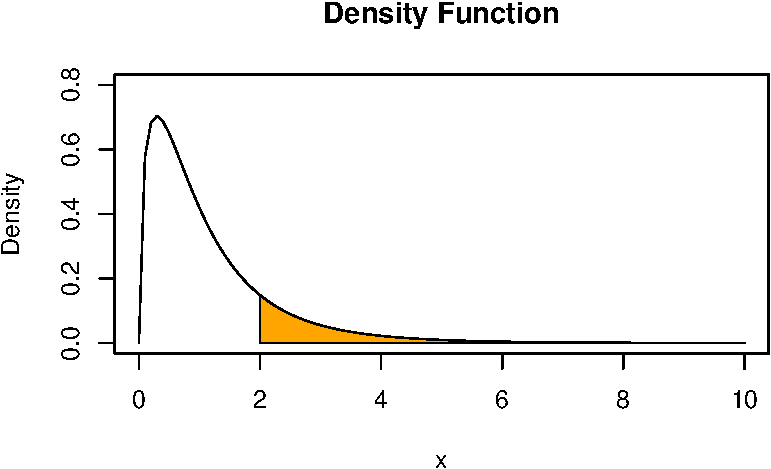
\includegraphics{ITER_files/figure-latex/unnamed-chunk-49-1} \end{center}

Since the outcomes of a \(\chi^2_M\) distributed random variable are
always positive, the support of the related PDF and CDF is
\(\mathbb{R}_{\geq0}\).

As expectation and variance depend (solely!) on the degrees of freedom,
the distribution's shape changes drastically if we vary the number of
squared standard normals that are summed up. This relation is often
depicted by overlaying densities for different \(M\), see the Wikipedia
Article.

We reproduce this here by plotting the density of the \(\chi_1^2\)
distribution on the interval \([0,15]\) with \texttt{curve()}. In the
next step, we loop over degrees of freedom \(M=2,...,7\) and add a
density curve for each \(M\) to the plot. We also adjust the line color
for each iteration of the loop by setting \texttt{col = M}. At last, we
add a legend that displays degrees of freedom and the associated colors.

\begin{Shaded}
\begin{Highlighting}[]
\CommentTok{# plot the density for M=1}
\KeywordTok{curve}\NormalTok{(}\KeywordTok{dchisq}\NormalTok{(x, }\DataTypeTok{df =} \DecValTok{1}\NormalTok{), }
      \DataTypeTok{xlim =} \KeywordTok{c}\NormalTok{(}\DecValTok{0}\NormalTok{, }\DecValTok{15}\NormalTok{), }
      \DataTypeTok{xlab =} \StringTok{"x"}\NormalTok{, }
      \DataTypeTok{ylab =} \StringTok{"Density"}\NormalTok{, }
      \DataTypeTok{main =} \StringTok{"Chi-Square Distributed Random Variables"}\NormalTok{)}

\CommentTok{# add densities for M=2,...,7 to the plot using a 'for()' loop }
\ControlFlowTok{for}\NormalTok{ (M }\ControlFlowTok{in} \DecValTok{2}\OperatorTok{:}\DecValTok{7}\NormalTok{) \{}
  \KeywordTok{curve}\NormalTok{(}\KeywordTok{dchisq}\NormalTok{(x, }\DataTypeTok{df =}\NormalTok{ M),}
        \DataTypeTok{xlim =} \KeywordTok{c}\NormalTok{(}\DecValTok{0}\NormalTok{, }\DecValTok{15}\NormalTok{), }
        \DataTypeTok{add =}\NormalTok{ T, }
        \DataTypeTok{col =}\NormalTok{ M)}
\NormalTok{\}}

\CommentTok{# add a legend}
\KeywordTok{legend}\NormalTok{(}\StringTok{"topright"}\NormalTok{, }
       \KeywordTok{as.character}\NormalTok{(}\DecValTok{1}\OperatorTok{:}\DecValTok{7}\NormalTok{), }
       \DataTypeTok{col =} \DecValTok{1}\OperatorTok{:}\DecValTok{7}\NormalTok{ , }
       \DataTypeTok{lty =} \DecValTok{1}\NormalTok{, }
       \DataTypeTok{title =} \StringTok{"D.F."}\NormalTok{)}
\end{Highlighting}
\end{Shaded}

\begin{center}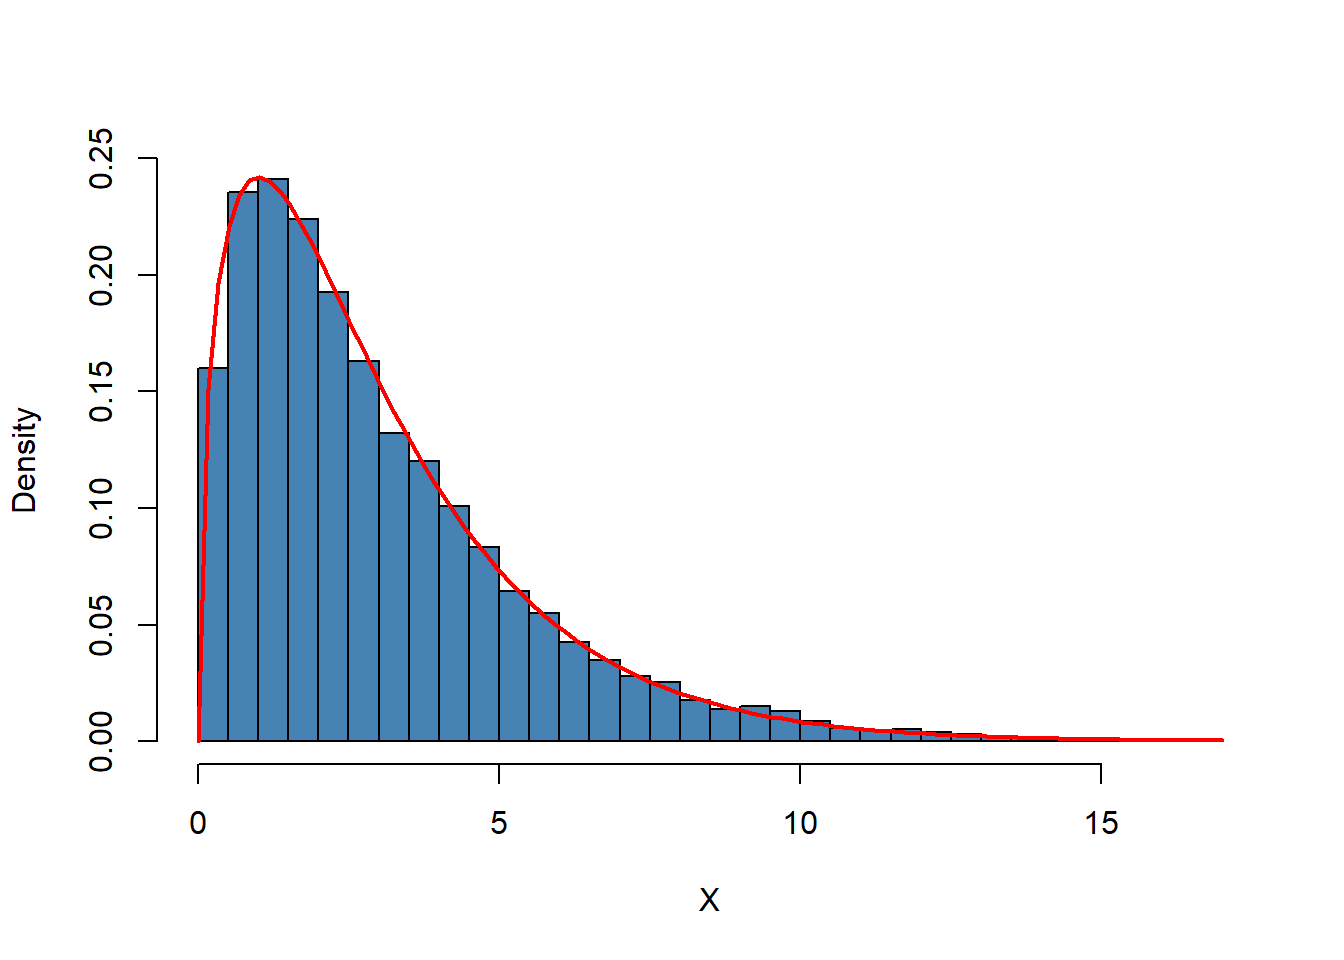
\includegraphics{ITER_files/figure-latex/unnamed-chunk-50-1} \end{center}

Increasing the degrees of freedom shifts the distribution to the right
(the mode becomes larger) and increases the dispersion (the
distribution's variance grows).

\hypertarget{thetdist}{\subsection*{The Student t
Distribution}\label{thetdist}}
\addcontentsline{toc}{subsection}{The Student t Distribution}

Let \(Z\) be a standard normal variate, \(W\) a \(\chi^2_M\) random
variable and further assume that \(Z\) and \(W\) are independent. Then
it holds that

\[ \frac{Z}{\sqrt{W/M}} =:X \sim t_M \] and \(X\) follows a
\emph{Student \(t\) distribution} (or simply \(t\) distribution) with
\(M\) degrees of freedom.

Similar to the \(\chi^2_M\) distribution, the shape of a \(t_M\)
distribution depends on \(M\). \(t\) distributions are symmetric,
bell-shaped and look similar to a normal distribution, especially when
\(M\) is large. This is not a coincidence: for a sufficiently large
\(M\), the \(t_M\) distribution can be approximated by the standard
normal distribution. This approximation works reasonably well for
\(M\geq 30\). As we will illustrate later by means of a small simulation
study, the \(t_{\infty}\) distribution \emph{is} the standard normal
distribution.

A \(t_M\) distributed random variable \(X\) has an expectation if
\(M>1\) and it has a variance if \(M>2\).

\begin{align}
  E(X) =& 0, \ M>1 \\
  \text{Var}(X) =& \frac{M}{M-2}, \ M>2
\end{align}

Let us plot some \(t\) distributions with different \(M\) and compare
them to the standard normal distribution.

\begin{Shaded}
\begin{Highlighting}[]
\CommentTok{# plot the standard normal density}
\KeywordTok{curve}\NormalTok{(}\KeywordTok{dnorm}\NormalTok{(x), }
      \DataTypeTok{xlim =} \KeywordTok{c}\NormalTok{(}\OperatorTok{-}\DecValTok{4}\NormalTok{, }\DecValTok{4}\NormalTok{), }
      \DataTypeTok{xlab =} \StringTok{"x"}\NormalTok{, }
      \DataTypeTok{lty =} \DecValTok{2}\NormalTok{, }
      \DataTypeTok{ylab =} \StringTok{"Density"}\NormalTok{, }
      \DataTypeTok{main =} \StringTok{"Densities of t Distributions"}\NormalTok{)}

\CommentTok{# plot the t density for M=2}
\KeywordTok{curve}\NormalTok{(}\KeywordTok{dt}\NormalTok{(x, }\DataTypeTok{df =} \DecValTok{2}\NormalTok{), }
      \DataTypeTok{xlim =} \KeywordTok{c}\NormalTok{(}\OperatorTok{-}\DecValTok{4}\NormalTok{, }\DecValTok{4}\NormalTok{), }
      \DataTypeTok{col =} \DecValTok{2}\NormalTok{, }
      \DataTypeTok{add =}\NormalTok{ T)}

\CommentTok{# plot the t density for M=4}
\KeywordTok{curve}\NormalTok{(}\KeywordTok{dt}\NormalTok{(x, }\DataTypeTok{df =} \DecValTok{4}\NormalTok{), }
      \DataTypeTok{xlim =} \KeywordTok{c}\NormalTok{(}\OperatorTok{-}\DecValTok{4}\NormalTok{, }\DecValTok{4}\NormalTok{), }
      \DataTypeTok{col =} \DecValTok{3}\NormalTok{, }
      \DataTypeTok{add =}\NormalTok{ T)}

\CommentTok{# plot the t density for M=25}
\KeywordTok{curve}\NormalTok{(}\KeywordTok{dt}\NormalTok{(x, }\DataTypeTok{df =} \DecValTok{25}\NormalTok{), }
      \DataTypeTok{xlim =} \KeywordTok{c}\NormalTok{(}\OperatorTok{-}\DecValTok{4}\NormalTok{, }\DecValTok{4}\NormalTok{), }
      \DataTypeTok{col =} \DecValTok{4}\NormalTok{, }
      \DataTypeTok{add =}\NormalTok{ T)}

\CommentTok{# add a legend}
\KeywordTok{legend}\NormalTok{(}\StringTok{"topright"}\NormalTok{, }
       \KeywordTok{c}\NormalTok{(}\StringTok{"N(0, 1)"}\NormalTok{, }\StringTok{"M=2"}\NormalTok{, }\StringTok{"M=4"}\NormalTok{, }\StringTok{"M=25"}\NormalTok{), }
       \DataTypeTok{col =} \DecValTok{1}\OperatorTok{:}\DecValTok{4}\NormalTok{, }
       \DataTypeTok{lty =} \KeywordTok{c}\NormalTok{(}\DecValTok{2}\NormalTok{, }\DecValTok{1}\NormalTok{, }\DecValTok{1}\NormalTok{, }\DecValTok{1}\NormalTok{))}
\end{Highlighting}
\end{Shaded}

\begin{center}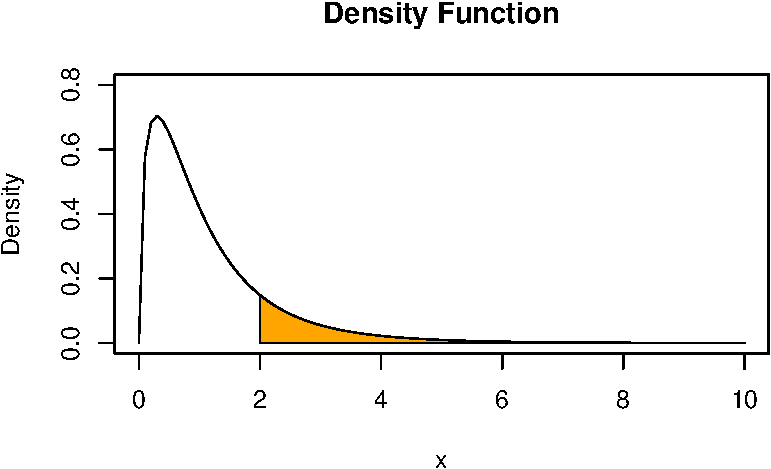
\includegraphics{ITER_files/figure-latex/unnamed-chunk-51-1} \end{center}

The plot illustrates what has been said in the previous paragraph: as
the degrees of freedom increase, the shape of the \(t\) distribution
comes closer to that of a standard normal bell curve. Already for
\(M=25\) we find little difference to the standard normal density. If
\(M\) is small, we find the distribution to have heavier tails than a
standard normal, i.e., it has a ``fatter'' bell shape.

\subsection*{The F Distribution}\label{the-f-distribution}
\addcontentsline{toc}{subsection}{The F Distribution}

Another ratio of random variables important to econometricians is the
ratio of two independent \(\chi^2\) distributed random variables that
are divided by their degrees of freedom \(M\) and \(n\). The quantity

\[ \frac{W/M}{V/n} \sim F_{M,n} \ \ \text{with} \ \ W \sim \chi^2_M \ \ , \ \ V \sim \chi^2_n \]
follows an \(F\) distribution with numerator degrees of freedom \(M\)
and denominator degrees of freedom \(n\), denoted \(F_{M,n}\). The
distribution was first derived by George Snedecor but was named in honor
of \href{https://en.wikipedia.org/wiki/Ronald_Fisher}{Sir Ronald
Fisher}.

By definition, the support of both PDF and CDF of an \(F_{M,n}\)
distributed random variable is \(\mathbb{R}_{\geq0}\).

Say we have an \(F\) distributed random variable \(Y\) with numerator
degrees of freedom \(3\) and denominator degrees of freedom \(14\) and
are interested in \(P(Y \geq 2)\). This can be computed with help of the
function \texttt{pf()}. By setting the argument \texttt{lower.tail} to
\texttt{TRUE} we ensure that \texttt{R} computes \(1- P(Y \leq 2)\),
i.e,the probability mass in the tail right of \(2\).

\begin{Shaded}
\begin{Highlighting}[]
\KeywordTok{pf}\NormalTok{(}\DecValTok{2}\NormalTok{, }\DecValTok{3}\NormalTok{, }\DecValTok{13}\NormalTok{, }\DataTypeTok{lower.tail =}\NormalTok{ F)}
\end{Highlighting}
\end{Shaded}

\begin{verbatim}
## [1] 0.1638271
\end{verbatim}

We can visualize this probability by drawing a line plot of the related
density and adding a color shading with \texttt{polygon()}.

\begin{Shaded}
\begin{Highlighting}[]
\CommentTok{# define coordinate vectors for vertices of the polygon}
\NormalTok{x <-}\StringTok{ }\KeywordTok{c}\NormalTok{(}\DecValTok{2}\NormalTok{, }\KeywordTok{seq}\NormalTok{(}\DecValTok{2}\NormalTok{, }\DecValTok{10}\NormalTok{, }\FloatTok{0.01}\NormalTok{), }\DecValTok{10}\NormalTok{)}
\NormalTok{y <-}\StringTok{ }\KeywordTok{c}\NormalTok{(}\DecValTok{0}\NormalTok{, }\KeywordTok{df}\NormalTok{(}\KeywordTok{seq}\NormalTok{(}\DecValTok{2}\NormalTok{, }\DecValTok{10}\NormalTok{, }\FloatTok{0.01}\NormalTok{), }\DecValTok{3}\NormalTok{, }\DecValTok{14}\NormalTok{), }\DecValTok{0}\NormalTok{)}

\CommentTok{# draw density of F_\{3, 14\}}
\KeywordTok{curve}\NormalTok{(}\KeywordTok{df}\NormalTok{(x ,}\DecValTok{3}\NormalTok{ ,}\DecValTok{14}\NormalTok{), }
      \DataTypeTok{ylim =} \KeywordTok{c}\NormalTok{(}\DecValTok{0}\NormalTok{, }\FloatTok{0.8}\NormalTok{), }
      \DataTypeTok{xlim =} \KeywordTok{c}\NormalTok{(}\DecValTok{0}\NormalTok{, }\DecValTok{10}\NormalTok{), }
      \DataTypeTok{ylab =} \StringTok{"Density"}\NormalTok{,}
      \DataTypeTok{main =} \StringTok{"Density Function"}\NormalTok{)}

\CommentTok{# draw the polygon}
\KeywordTok{polygon}\NormalTok{(x, y, }\DataTypeTok{col =} \StringTok{"orange"}\NormalTok{)}
\end{Highlighting}
\end{Shaded}

\begin{center}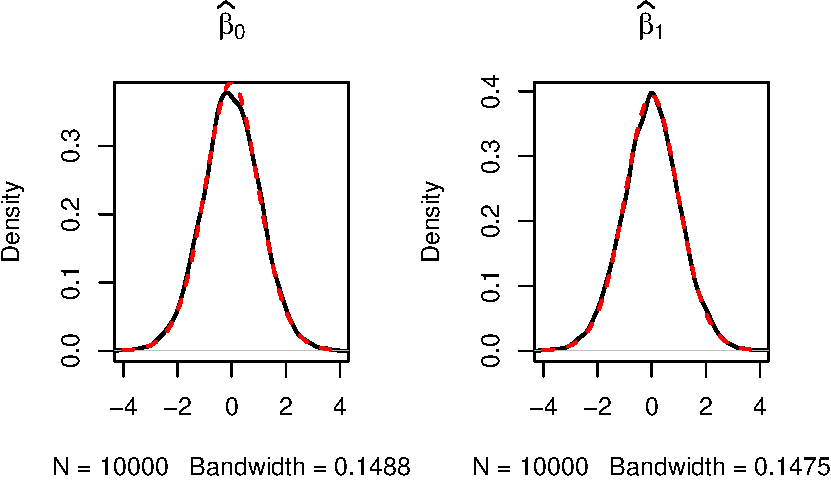
\includegraphics{ITER_files/figure-latex/unnamed-chunk-53-1} \end{center}

The \(F\) distribution is related to many other distributions. An
important special case encountered in econometrics arises if the
denominator degrees of freedom are large such that the \(F_{M,n}\)
distribution can be approximated by the \(F_{M,\infty}\) distribution
which turns out to be simply the distribution of a \(\chi^2_M\) random
variable divided by its degrees of freedom \(M\),

\[ W/M \sim F_{M,\infty} \ \ , \ \ W \sim \chi^2_M. \]

\section{Random Sampling and the Distribution of Sample
Averages}\label{RSATDOSA}

To clarify the basic idea of random sampling, let us jump back to the
dice rolling example:

Suppose we are rolling the dice \(n\) times. This means we are
interested in the outcomes of random \(Y_i, \ i=1,...,n\) which are
characterized by the same distribution. Since these outcomes are
selected randomly, they are \emph{random variables} themselves and their
realizations will differ each time we draw a sample, i.e., each time we
roll the dice \(n\) times. Furthermore, each observation is randomly
drawn from the same population, that is, the numbers from \(1\) to
\(6\), and their individual distribution is the same. Hence
\(Y_1,\dots,Y_n\) are identically distributed.

Moreover, we know that the value of any of the \(Y_i\) does not provide
any information on the remainder of the outcomes In our example, rolling
a six as the first observation in our sample does not alter the
distributions of \(Y_2,\dots,Y_n\): all numbers are equally likely to
occur. This means that all \(Y_i\) are also independently distributed.
Thus \(Y_1,\dots,Y_n\) are independently and identically distributed
(\emph{i.i.d.}). The dice example uses this most simple sampling scheme.
That is why it is called \emph{simple random sampling}. This concept is
summarized in Key Concept 2.5.

\begin{keyconcepts}[Simple Random Sampling and i.i.d. Random Variables]{2.5}
In simple random sampling, $n$ objects are drawn at random from a population. Each object is equally likely to end up in the sample. We denote the value of the random variable $Y$ for the $i^{th}$ randomly drawn object as $Y_i$.  Since all objects are equally likely to be drawn and the distribution of $Y_i$ is the same for all $i$, the $Y_i, \dots, Y_n$ are independently and identically distributed (i.i.d.). This means the distribution of $Y_i$ is the same for all $i=1,\dots,n$ and $Y_1$ is distributed independently of $Y_2, \dots, Y_n$ and $Y_2$ is distributed independently of $Y_1, Y_3, \dots, Y_n$ and so forth.
\end{keyconcepts}

What happens if we consider functions of the sample data? Consider the
example of rolling a dice two times in a row once again. A sample now
consists of two independent random draws from the set
\(\{1,2,3,4,5,6\}\). In view of the afore, it is apparent that any
function of these two random variables is also random, e.g., their sum.
Convince yourself by executing the code below several times.

\begin{Shaded}
\begin{Highlighting}[]
\KeywordTok{sum}\NormalTok{(}\KeywordTok{sample}\NormalTok{(}\DecValTok{1}\OperatorTok{:}\DecValTok{6}\NormalTok{, }\DecValTok{2}\NormalTok{, }\DataTypeTok{replace =}\NormalTok{ T))}
\end{Highlighting}
\end{Shaded}

\begin{verbatim}
## [1] 6
\end{verbatim}

Clearly, this sum, let us call it \(S\), is a random variable as it
depends on randomly drawn summands. For this example, we can completely
enumerate all outcomes and hence write down the theoretical probability
distribution of our function of the sample data, \(S\):

We face \(6^2=36\) possible pairs. Those pairs are

\begin{align*}
  &(1,1)    (1,2)   (1,3)   (1,4)   (1,5)   (1,6) \\ 
  &(2,1)    (2,2)   (2,3)   (2,4)   (2,5)   (2,6) \\ 
  &(3,1)    (3,2)   (3,3)   (3,4)   (3,5)   (3,6) \\ 
  &(4,1)    (4,2)   (4,3)   (4,4)   (4,5)   (4,6) \\ 
  &(5,1)    (5,2)   (5,3)   (5,4)   (5,5)   (5,6) \\ 
  &(6,1)    (6,2)   (6,3)   (6,4)   (6,5)   (6,6)
\end{align*}

Thus, possible outcomes for \(S\) are

\[ \left\{ 2,3,4,5,6,7,8,9,10,11,12 \right\} . \] Enumeration of
outcomes yields

\begin{align}
  P(S) = 
  \begin{cases} 
    1/36, \ & S = 2 \\ 
    2/36, \ & S = 3 \\
    3/36, \ & S = 4 \\
    4/36, \ & S = 5 \\
    5/36, \ & S = 6 \\
    6/36, \ & S = 7 \\
    5/36, \ & S = 8 \\
    4/36, \ & S = 9 \\
    3/36, \ & S = 10 \\
    2/36, \ & S = 11 \\
    1/36, \ & S = 12
  \end{cases}
\end{align}

We can also compute \(E(S)\) and \(\text{Var}(S)\) as stated in Key
Concept 2.1 and Key Concept 2.2.

\begin{Shaded}
\begin{Highlighting}[]
\CommentTok{# Vector of outcomes}
\NormalTok{S <-}\StringTok{ }\DecValTok{2}\OperatorTok{:}\DecValTok{12}

\CommentTok{# Vector of probabilities}
\NormalTok{PS <-}\StringTok{ }\KeywordTok{c}\NormalTok{(}\DecValTok{1}\OperatorTok{:}\DecValTok{6}\NormalTok{, }\DecValTok{5}\OperatorTok{:}\DecValTok{1}\NormalTok{) }\OperatorTok{/}\StringTok{ }\DecValTok{36}

\CommentTok{# Expectation of S}
\NormalTok{ES <-}\StringTok{ }\NormalTok{S }\OperatorTok\StringTok{ }\NormalTok{PS}
\NormalTok{ES}
\end{Highlighting}
\end{Shaded}

\begin{verbatim}
##      [,1]
## [1,]    7
\end{verbatim}

\begin{Shaded}
\begin{Highlighting}[]
\CommentTok{# Variance of S}
\NormalTok{VarS <-}\StringTok{ }\NormalTok{(S }\OperatorTok{-}\StringTok{ }\KeywordTok{c}\NormalTok{(ES))}\OperatorTok{^}\DecValTok{2} \OperatorTok\StringTok{ }\NormalTok{PS}
\NormalTok{VarS}
\end{Highlighting}
\end{Shaded}

\begin{verbatim}
##          [,1]
## [1,] 5.833333
\end{verbatim}

The \texttt{\%*\%} operator is used to compute the scalar product of two
vectors.

So the distribution of \(S\) is known. It is also evident that its
distribution differs considerably from the marginal distribution,
i.e,the distribution of a single dice roll's outcome, \(D\) . Let us
visualize this using bar plots.

\begin{Shaded}
\begin{Highlighting}[]
\CommentTok{# divide the plotting area into one row with two columns}
\KeywordTok{par}\NormalTok{(}\DataTypeTok{mfrow =} \KeywordTok{c}\NormalTok{(}\DecValTok{1}\NormalTok{, }\DecValTok{2}\NormalTok{))}

\CommentTok{# plot the distribution of S}
\KeywordTok{barplot}\NormalTok{(PS, }
        \DataTypeTok{ylim =} \KeywordTok{c}\NormalTok{(}\DecValTok{0}\NormalTok{, }\FloatTok{0.2}\NormalTok{), }
        \DataTypeTok{xlab =} \StringTok{"S"}\NormalTok{, }
        \DataTypeTok{ylab =} \StringTok{"Probability"}\NormalTok{, }
        \DataTypeTok{col =} \StringTok{"steelblue"}\NormalTok{, }
        \DataTypeTok{space =} \DecValTok{0}\NormalTok{, }
        \DataTypeTok{main =} \StringTok{"Sum of Two Dice Rolls"}\NormalTok{)}

\CommentTok{# plot the distribution of D }
\NormalTok{probability <-}\StringTok{ }\KeywordTok{rep}\NormalTok{(}\DecValTok{1}\OperatorTok{/}\DecValTok{6}\NormalTok{, }\DecValTok{6}\NormalTok{)}
\KeywordTok{names}\NormalTok{(probability) <-}\StringTok{ }\DecValTok{1}\OperatorTok{:}\DecValTok{6}

\KeywordTok{barplot}\NormalTok{(probability, }
        \DataTypeTok{ylim =} \KeywordTok{c}\NormalTok{(}\DecValTok{0}\NormalTok{, }\FloatTok{0.2}\NormalTok{), }
        \DataTypeTok{xlab =} \StringTok{"D"}\NormalTok{, }
        \DataTypeTok{col =} \StringTok{"steelblue"}\NormalTok{, }
        \DataTypeTok{space =} \DecValTok{0}\NormalTok{, }
        \DataTypeTok{main =} \StringTok{"Outcome of a Single Dice Roll"}\NormalTok{)}
\end{Highlighting}
\end{Shaded}

\begin{center}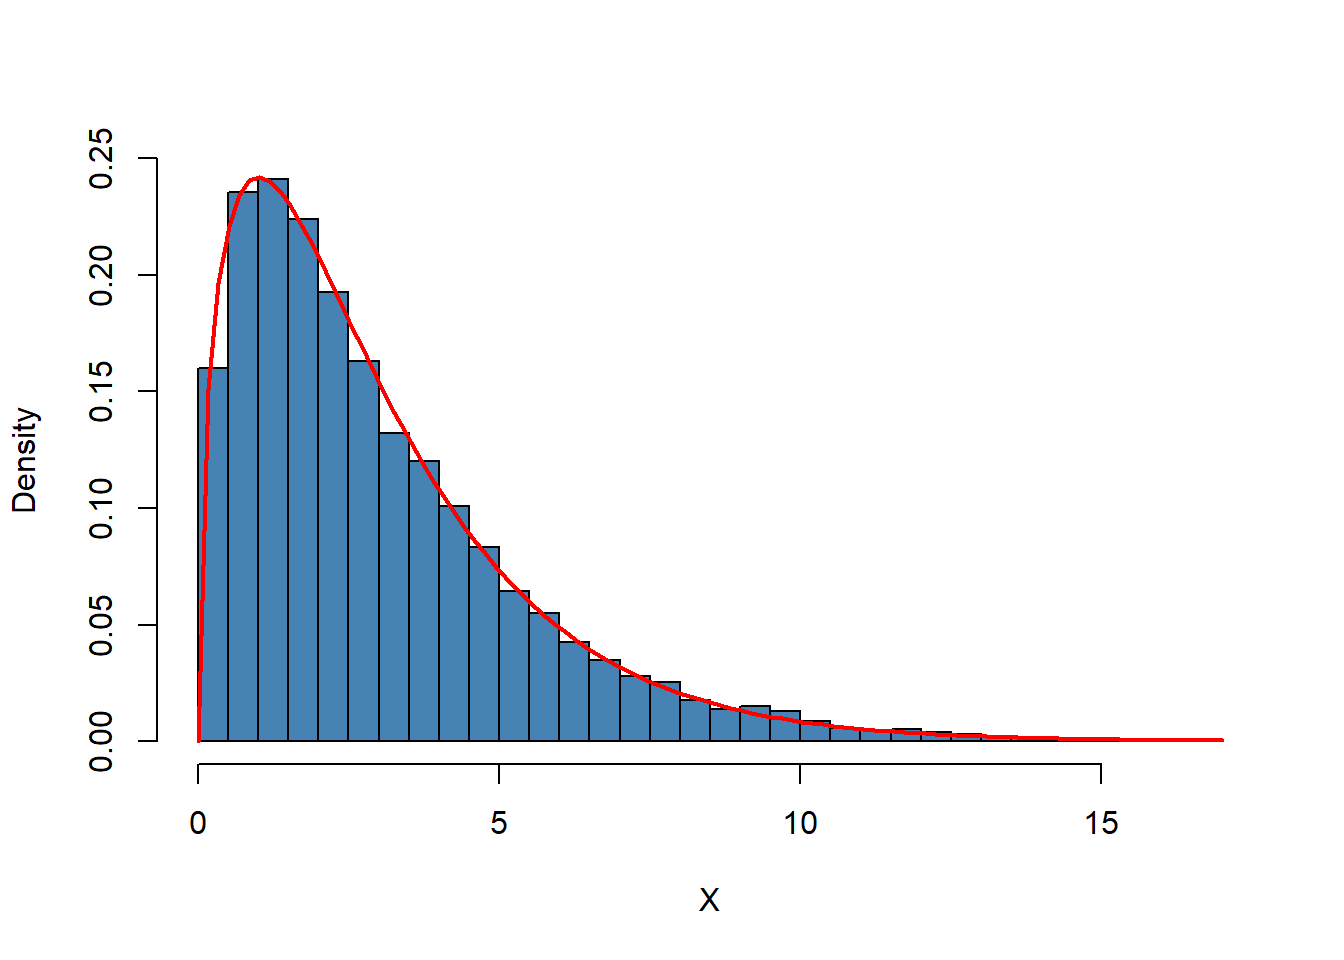
\includegraphics{ITER_files/figure-latex/unnamed-chunk-59-1} \end{center}

Many econometric procedures deal with averages of sampled data. It is
typically assumed that observations are drawn randomly from a larger,
unknown population. As demonstrated for the sample function \(S\),
computing an average of a random sample has the effect that the average
is a random variable itself. This random variable in turn has a
probability distribution, called the sampling distribution. Knowledge
about the sampling distribution of the average is therefore crucial for
understanding the performance of econometric procedures.

The \emph{sample average} of a sample of \(n\) observations
\(Y_1, \dots, Y_n\) is

\[ \overline{Y} = \frac{1}{n} \sum_{i=1}^n Y_i = \frac{1}{n} (Y_1 + Y_2 + \cdots + Y_n). \]
\(\overline{Y}\) is also called the sample mean.

\subsection*{Mean and Variance of the Sample
Mean}\label{mean-and-variance-of-the-sample-mean}
\addcontentsline{toc}{subsection}{Mean and Variance of the Sample Mean}

suppose that all observations \(Y_1,\dots,Y_n\) are i.i.d. and denote
\(\mu_Y\) and \(\sigma_Y^2\) the mean and the variance of the \(Y_i\).
Then we have that

\[ E(\overline{Y}) = E\left(\frac{1}{n} \sum_{i=1}^n Y_i \right) = \frac{1}{n} E\left(\sum_{i=1}^n Y_i\right) = \frac{1}{n} \sum_{i=1}^n E\left(Y_i\right) = \frac{1}{n} \cdot n \cdot \mu_Y = \mu_Y    \]
and

\begin{align*}
  \text{Var}(\overline{Y}) =& \text{Var}\left(\frac{1}{n} \sum_{i=1}^n Y_i \right) \\
  =& \frac{1}{n^2} \sum_{i=1}^n \text{Var}(Y_i) + \frac{1}{n^2} \sum_{i=1}^n \sum_{j=1, j\neq i}^n \text{cov}(Y_i,Y_j) \\
  =& \frac{\sigma^2_Y}{n} \\
  =& \sigma_{\overline{Y}}^2.
\end{align*}

The second summand vanishes since \(\text{cov}(Y_i,Y_j)=0\) for
\(i\neq j\) due to independence. Consequently, the standard deviation of
the sample mean is given by
\[\sigma_{\overline{Y}} = \frac{\sigma_Y}{\sqrt{n}}.\]

It is worthwhile to mention that these results hold irrespective of the
underlying distribution of the \(Y_i\).

\subsubsection*{\texorpdfstring{The Sampling Distribution of
\(\overline{Y}\) when \(Y\) Is Normally
Distributed}{The Sampling Distribution of \textbackslash{}overline\{Y\} when Y Is Normally Distributed}}\label{the-sampling-distribution-of-overliney-when-y-is-normally-distributed}
\addcontentsline{toc}{subsubsection}{The Sampling Distribution of
\(\overline{Y}\) when \(Y\) Is Normally Distributed}

If the \(Y_1,\dots,Y_n\) are i.i.d. draws from a normal distribution
with mean \(\mu_Y\) and variance \(\sigma_Y^2\), the following holds for
their sample average \(\overline{Y}\):

\[ \overline{Y} \sim \mathcal{N}(\mu_Y, \sigma_Y^2/n) \tag{2.4} \]

For example, if a sample \(Y_i\) with \(i=1,\dots,10\) is drawn from a
standard normal distribution with mean \(\mu_Y = 0\) and variance
\(\sigma_Y^2=1\) we have

\[ \overline{Y} \sim \mathcal{N}(0,0.1).\]

We can use \texttt{R}'s random number generation facilities to verify
this result. The basic idea is to simulate outcomes of the true
distribution of \(\overline{Y}\) by repeatedly drawing random samples of
10 observation from the \(\mathcal{N}(0,1)\) distribution and computing
their respective averages. If we do this for a large number of
repetitions, the simulated data set of averages should quite accurately
reflect the theoretical distribution of \(\overline{Y}\) if the
theoretical result holds.

The approach sketched above is an example of what is commonly known as
\emph{Monte Carlo Simulation} or \emph{Monte Carlo Experiment}. To
perform this simulation in \texttt{R}, we proceed as follows:

\begin{enumerate}
\def\labelenumi{\arabic{enumi}.}
\tightlist
\item
  Choose a sample size \texttt{n} and the number of samples to be drawn,
  \texttt{reps}.
\item
  Use the function \texttt{replicate()} in conjunction with
  \texttt{rnorm()} to draw \texttt{n} observations from the standard
  normal distribution \texttt{rep} times. \textbf{Note}: the outcome of
  \texttt{replicate()} is a matrix with dimensions \texttt{n} \(\times\)
  \texttt{rep}. It contains the drawn samples as \emph{columns}.
\item
  Compute sample means using \texttt{colMeans()}. This function computes
  the mean of each column, i.e., of each sample and returns a vector.
\end{enumerate}

\begin{Shaded}
\begin{Highlighting}[]
\CommentTok{# set sample size and number of samples}
\NormalTok{n <-}\StringTok{ }\DecValTok{10}
\NormalTok{reps <-}\StringTok{ }\DecValTok{10000}

\CommentTok{# perform random sampling}
\NormalTok{samples <-}\StringTok{ }\KeywordTok{replicate}\NormalTok{(reps, }\KeywordTok{rnorm}\NormalTok{(n)) }\CommentTok{# 10 x 10000 sample matrix}

\CommentTok{# compute sample means}
\NormalTok{sample.avgs <-}\StringTok{ }\KeywordTok{colMeans}\NormalTok{(samples)}
\end{Highlighting}
\end{Shaded}

We then end up with a vector of sample averages. You can check the
vector property of \texttt{sample.avgs}:

\begin{Shaded}
\begin{Highlighting}[]
\CommentTok{# check that 'sample.avgs' is a vector}
\KeywordTok{is.vector}\NormalTok{(sample.avgs) }
\end{Highlighting}
\end{Shaded}

\begin{verbatim}
## [1] TRUE
\end{verbatim}

\begin{Shaded}
\begin{Highlighting}[]
\CommentTok{# print the first few entries to the console}
\KeywordTok{head}\NormalTok{(sample.avgs)}
\end{Highlighting}
\end{Shaded}

\begin{verbatim}
## [1] -0.12406767 -0.10649421 -0.01033423 -0.39905236 -0.41897968 -0.90883537
\end{verbatim}

A straightforward approach to examine the distribution of univariate
numerical data is to plot it as a histogram and compare it to some known
or assumed distribution. By default, \texttt{hist()} will give us a
frequency histogram, i.e., a bar chart where observations are grouped
into ranges, also called bins. The ordinate reports the number of
observations falling into each of the bins. Instead, we want it to
report density estimates for comparison purposes. This is achieved by
setting the argument \texttt{freq = FALSE}. The number of bins is
adjusted by the argument \texttt{breaks}.

Using \texttt{curve()}, we overlay the histogram with a red line, the
theoretical density of a \(\mathcal{N}(0, 0.1)\) random variable.
Remember to use the argument \texttt{add = TRUE} to add the curve to the
current plot. Otherwise \texttt{R} will open a new graphic device and
discard the previous plot!\footnote{\emph{Hint:} \texttt{T} and
  \texttt{F} are alternatives for \texttt{TRUE} and \texttt{FALSE}.}

\begin{Shaded}
\begin{Highlighting}[]
\CommentTok{# Plot the density histogram}
\KeywordTok{hist}\NormalTok{(sample.avgs, }
     \DataTypeTok{ylim =} \KeywordTok{c}\NormalTok{(}\DecValTok{0}\NormalTok{, }\FloatTok{1.4}\NormalTok{), }
     \DataTypeTok{col =} \StringTok{"steelblue"}\NormalTok{ , }
     \DataTypeTok{freq =}\NormalTok{ F, }
     \DataTypeTok{breaks =} \DecValTok{20}\NormalTok{)}

\CommentTok{# overlay the theoretical distribution of sample averages on top of the histogram}
\KeywordTok{curve}\NormalTok{(}\KeywordTok{dnorm}\NormalTok{(x, }\DataTypeTok{sd =} \DecValTok{1}\OperatorTok{/}\KeywordTok{sqrt}\NormalTok{(n)), }
      \DataTypeTok{col =} \StringTok{"red"}\NormalTok{, }
      \DataTypeTok{lwd =} \StringTok{"2"}\NormalTok{, }
      \DataTypeTok{add =}\NormalTok{ T)}
\end{Highlighting}
\end{Shaded}

\begin{center}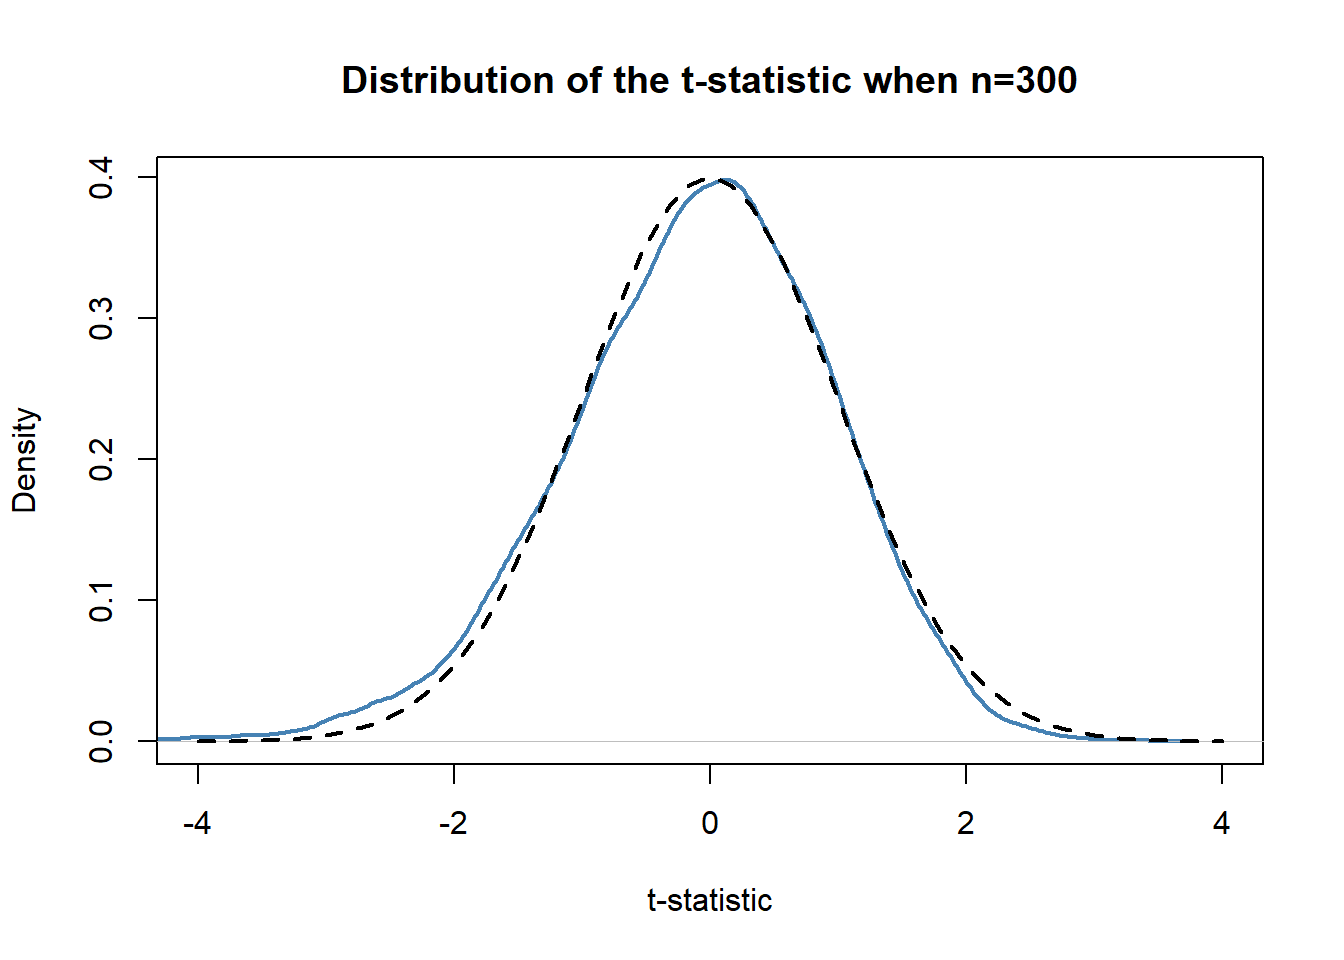
\includegraphics{ITER_files/figure-latex/unnamed-chunk-62-1} \end{center}

The sampling distribution of \(\overline{Y}\) is indeed very close to
that of a \(\mathcal{N}(0, 0.1)\) distribution so the Monte Carlo
Simulation supports the theoretical claim.

Let us discuss another example where using simple random sampling in a
simulation setup helps to verify a well known result. As discussed
before, the \protect\hyperlink{chisquare}{Chi-squared} distribution with
\(M\) degrees of freedom arises as the distribution of the sum of \(M\)
independent squared standard normal distributed random variables.

To visualize the claim stated in equation (2.3), we proceed similarly as
in the example before:

\begin{enumerate}
\def\labelenumi{\arabic{enumi}.}
\tightlist
\item
  Choose the degrees of freedom, \texttt{DF}, and the number of samples
  to be drawn \texttt{reps}.
\item
  Draw \texttt{reps} random samples of size \texttt{DF} from the
  standard normal distribution using \texttt{replicate()}.
\item
  For each sample, square the outcomes and sum them up column-wise.
  Store the results.
\end{enumerate}

Again, we produce a density estimate for the distribution underlying our
simulated data using a density histogram and overlay it with a line
graph of the theoretical density function of the \(\chi^2_3\)
distribution.

\begin{Shaded}
\begin{Highlighting}[]
\CommentTok{# number of repititions}
\NormalTok{reps <-}\StringTok{ }\DecValTok{10000}

\CommentTok{# set degrees of freedom of a chi-Square Distribution}
\NormalTok{DF <-}\StringTok{ }\DecValTok{3} 

\CommentTok{# sample 10000 column vectors à 3 N(0,1) R.V.S}
\NormalTok{Z <-}\StringTok{ }\KeywordTok{replicate}\NormalTok{(reps, }\KeywordTok{rnorm}\NormalTok{(DF)) }

\CommentTok{# column sums of squares}
\NormalTok{X <-}\StringTok{ }\KeywordTok{colSums}\NormalTok{(Z}\OperatorTok{^}\DecValTok{2}\NormalTok{)}

\CommentTok{# histogram of column sums of squares}
\KeywordTok{hist}\NormalTok{(X, }
     \DataTypeTok{freq =}\NormalTok{ F, }
     \DataTypeTok{col =} \StringTok{"steelblue"}\NormalTok{, }
     \DataTypeTok{breaks =} \DecValTok{40}\NormalTok{, }
     \DataTypeTok{ylab =} \StringTok{"Density"}\NormalTok{, }
     \DataTypeTok{main =} \StringTok{""}\NormalTok{)}

\CommentTok{# add theoretical density}
\KeywordTok{curve}\NormalTok{(}\KeywordTok{dchisq}\NormalTok{(x, }\DataTypeTok{df =}\NormalTok{ DF), }
      \DataTypeTok{type =} \StringTok{'l'}\NormalTok{, }
      \DataTypeTok{lwd =} \DecValTok{2}\NormalTok{, }
      \DataTypeTok{col =} \StringTok{"red"}\NormalTok{, }
      \DataTypeTok{add =}\NormalTok{ T)}
\end{Highlighting}
\end{Shaded}

\begin{center}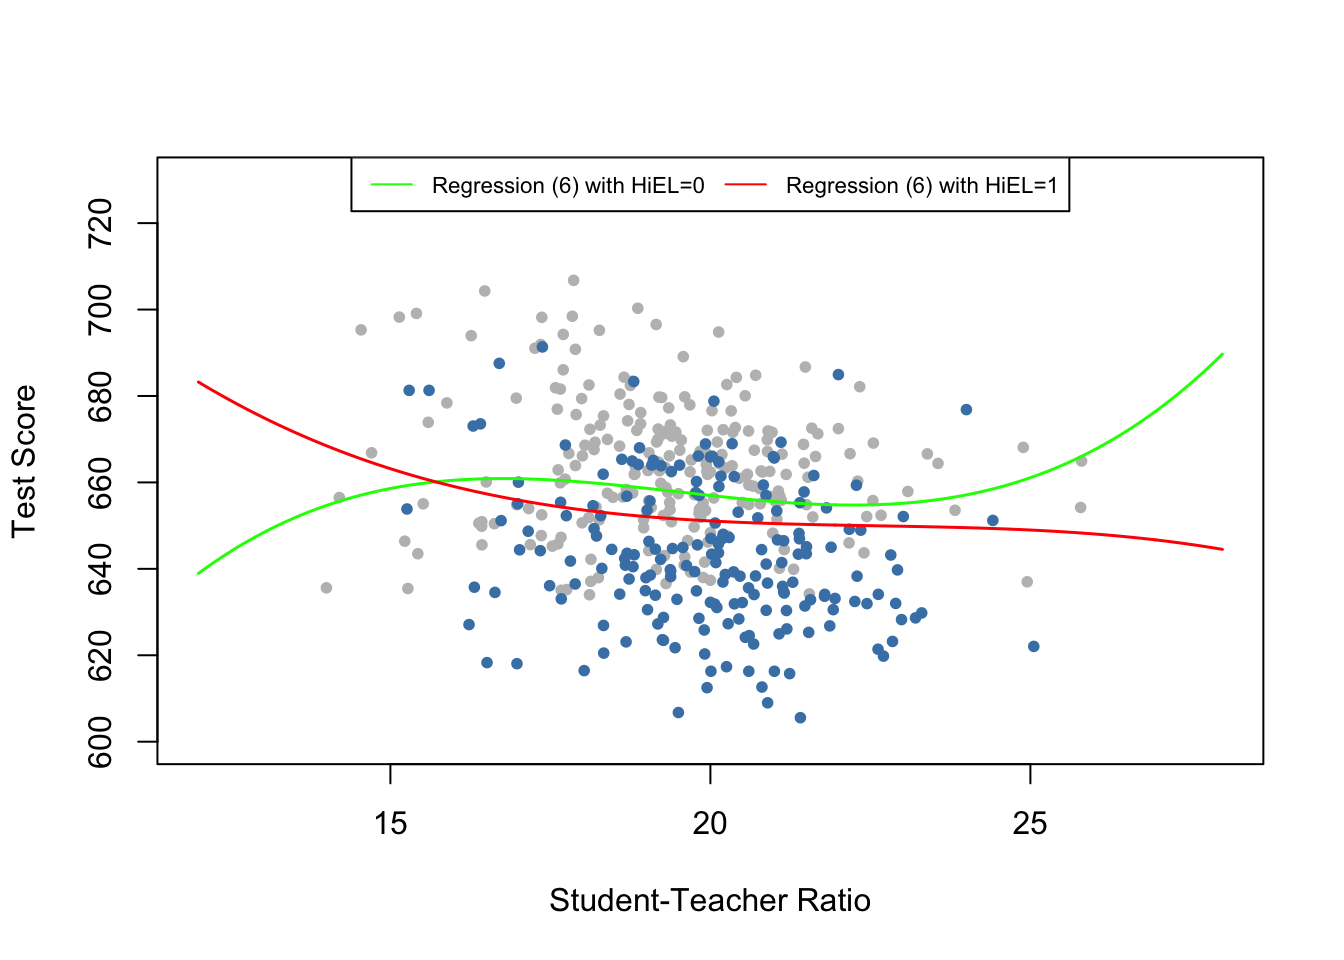
\includegraphics{ITER_files/figure-latex/unnamed-chunk-63-1} \end{center}

\subsection*{Large Sample Approximations to Sampling
Distributions}\label{large-sample-approximations-to-sampling-distributions}
\addcontentsline{toc}{subsection}{Large Sample Approximations to
Sampling Distributions}

Sampling distributions as considered in the last section play an
important role in the development of econometric methods. There are two
main approaches in characterizing sampling distributions: an ``exact''
approach and an ``approximate'' approach.

The exact approach aims to find a general formula for the sampling
distribution that holds for any sample size \(n\). We call this the
\emph{exact distribution} or \emph{finite-sample distribution}. In the
previous examples of dice rolling and normal variates, we have dealt
with functions of random variables whose sample distributions are
\emph{excactly known} in the sense that we can write them down as
analytic expressions. However, this is not always possible. For
\(\overline{Y}\), result (2.4) tells us that normality of the \(Y_i\)
implies normality of \(\overline{Y}\) (we demonstrated this for the
special case of \(Y_i \overset{i.i.d.}{\sim} \mathcal{N}(0,1)\) with
\(n=10\) using a simulation study that involves simple random sampling).
Unfortunately, the \emph{exact} distribution of \(\overline{Y}\) is
generally unknown and often hard to derive (or even untraceable) if we
drop the assumption that the \(Y_i\) have a normal distribution.

Therefore, as can be guessed from its name, the ``approximate'' approach
aims to find an approximation to the sampling distribution where it is
required that the sample size \(n\) is large. A distribution that is
used as a large-sample approximation to the sampling distribution is
also called the \emph{asymptotic distribution}. This is due to the fact
that the asymptotic distribution \emph{is} the sampling distribution for
\(n \rightarrow \infty\), i.e., the approximation becomes exact if the
sample size goes to infinity. However, the difference between the
sampling distribution and the asymptotic distribution is negligible for
moderate or even small samples sizes so that approximations using the
asymptotic distribution are useful.

In this section we will discuss two well known results that are used to
approximate sampling distributions and thus constitute key tools in
econometric theory: the \emph{law of large numbers} and the
\emph{central limit theorem}. The law of large numbers states that in
large samples, \(\overline{Y}\) is close to \(\mu_Y\) with high
probability. The central limit theorem says that the sampling
distribution of the standardized sample average, that is,
\((\overline{Y} - \mu_Y)/\sigma_{\overline{Y}}\) is asymptotically
normally distributed. It is particularly interesting that both results
do not depend on the distribution of \(Y\). In other words, being unable
to describe the complicated sampling distribution of \(\overline{Y}\) if
\(Y\) is not normal, approximations of the latter using the central
limit theorem simplify the development and applicability of econometric
procedures enormously. This is a key component underlying the theory of
statistical inference for regression models. Both results are summarized
in Key Concept 2.6 and Key Concept 2.7.

\begin{keyconcepts}[Convergence in Probability\comma Consistency and the Law of Large Numbers]{2.6}
The sample average $\overline{Y}$ converges in probability to $\mu_Y$: $\overline{Y}$ is \textit{consistent} for $\mu_Y$ if the probability that $\overline{Y}$ is in the range $(\mu_Y - \epsilon)$ to $(\mu_Y + \epsilon)$ becomes arbitrary close to $1$ as $n$ increases for any constant $\epsilon > 0$. We write this as

$$ \overline{Y} \xrightarrow[]{p} \mu_Y. $$

Consider the independently and identically distributed random variables $Y_i, i=1,\dots,n$ with expectation $E(Y_i)=\mu_Y$ and variance $\text{Var}(Y_i)=\sigma^2_Y$. Under the condition that $\sigma^2_Y< \infty$, that is, large outliers are unlikely, the law of large numbers states

$$ \overline{Y} \xrightarrow[]{p} \mu_Y. $$

The following application simulates a large number of coin tosses (you may set the number of trials using the slider) with a fair coin and computes the fraction of heads observed for each additional toss. The result is a random path that, as stated by the law of large numbers, shows a tendency to approach the value of $0.5$ as $n$ grows.\newline
\begin{center}
\textit{This interactive application is only available in the HTML version.}
\end{center}
\end{keyconcepts}

The core statement of the law of large numbers is that under quite
general conditions, the probability of obtaining a sample average
\(\overline{Y}\) that is close to \(\mu_Y\) is high if we have a large
sample size.

Consider the example of repeatedly tossing a coin where \(Y_i\) is the
result of the \(i^{th}\) coin toss. \(Y_i\) is a Bernoulli distributed
random variable with \(p\) the probability of observing head
\[ P(Y_i) = \begin{cases} p, & Y_i = 1 \\ 1-p, & Y_i = 0 \end{cases} \]
where \(p = 0.5\) as we assume a fair coin. It is straightforward to
show that

\[ \mu_Y = p = 0.5. \] Let \(R_n\) denote the proportion of heads in the
first \(n\) tosses,

\[ R_n = \frac{1}{n} \sum_{i=1}^n Y_i. \tag{2.5}\]

According to the law of large numbers, the observed proportion of heads
converges in probability to \(\mu_Y = 0.5\), the probability of tossing
head in a \emph{single} coin toss,
\[ R_n \xrightarrow[]{p} \mu_Y=0.5 \ \ \text{as} \ \ n \rightarrow \infty.\]
This result is the as the one illustrated by the interactive application
in Key Concept 2.6. We now show how to replicate this using \texttt{R}.

The procedure is as follows:

\begin{enumerate}
\def\labelenumi{\arabic{enumi}.}
\tightlist
\item
  Sample \texttt{N} observations from the Bernoulli distribution, e.g.,
  using \texttt{sample()}.
\item
  Calculate the proportion of heads \(R_n\) as in (2.5). A way to
  achieve this is to call \texttt{cumsum()} on the vector of
  observations \texttt{Y} to obtain its cumulative sum and then divide
  by the respective number of observations.
\end{enumerate}

We continue by plotting the path and also add a dashed line for the
benchmark probability \(p = 0.5\).

\begin{Shaded}
\begin{Highlighting}[]
\CommentTok{# set seed}
\KeywordTok{set.seed}\NormalTok{(}\DecValTok{1}\NormalTok{)}

\CommentTok{# set number of coin tosses and simulate}
\NormalTok{N <-}\StringTok{ }\DecValTok{30000}
\NormalTok{Y <-}\StringTok{ }\KeywordTok{sample}\NormalTok{(}\DecValTok{0}\OperatorTok{:}\DecValTok{1}\NormalTok{, N, }\DataTypeTok{replace =}\NormalTok{ T)}

\CommentTok{# Calculate R_n for 1:N}
\NormalTok{S <-}\StringTok{ }\KeywordTok{cumsum}\NormalTok{(Y)}
\NormalTok{R <-}\StringTok{ }\NormalTok{S}\OperatorTok{/}\NormalTok{(}\DecValTok{1}\OperatorTok{:}\NormalTok{N)}

\CommentTok{# Plot the path.}
\KeywordTok{plot}\NormalTok{(R, }
     \DataTypeTok{ylim =} \KeywordTok{c}\NormalTok{(}\FloatTok{0.3}\NormalTok{, }\FloatTok{0.7}\NormalTok{), }
     \DataTypeTok{type =} \StringTok{"l"}\NormalTok{, }
     \DataTypeTok{col =} \StringTok{"steelblue"}\NormalTok{, }
     \DataTypeTok{lwd =} \DecValTok{2}\NormalTok{, }
     \DataTypeTok{xlab =} \StringTok{"n"}\NormalTok{, }
     \DataTypeTok{ylab =} \StringTok{"R_n"}\NormalTok{,}
     \DataTypeTok{main =} \StringTok{"Converging Share of Heads in Repeated Coin Tossing"}\NormalTok{)}

\CommentTok{# Add a dashed line for R_n = 0.5}
\KeywordTok{lines}\NormalTok{(}\KeywordTok{c}\NormalTok{(}\DecValTok{0}\NormalTok{, N), }
      \KeywordTok{c}\NormalTok{(}\FloatTok{0.5}\NormalTok{, }\FloatTok{0.5}\NormalTok{), }
      \DataTypeTok{col =} \StringTok{"darkred"}\NormalTok{, }
      \DataTypeTok{lty =} \DecValTok{2}\NormalTok{, }
      \DataTypeTok{lwd =} \DecValTok{1}\NormalTok{)}
\end{Highlighting}
\end{Shaded}

\begin{center}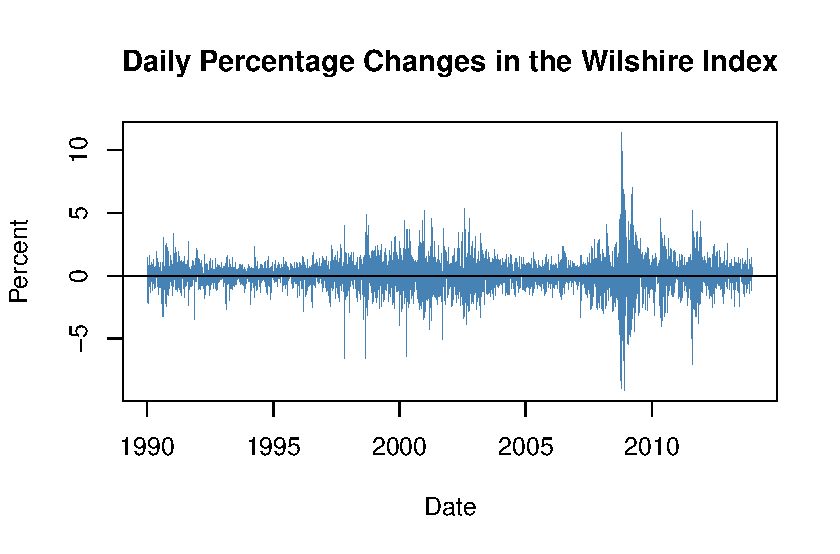
\includegraphics{ITER_files/figure-latex/unnamed-chunk-66-1} \end{center}

There are several things to be said about this plot.

\begin{itemize}
\item
  The blue graph shows the observed proportion of heads when tossing a
  coin \(n\) times.
\item
  Since the \(Y_i\) are random variables, \(R_n\) is a random variate,
  too. The path depicted is only one of many possible realizations of
  \(R_n\) as it is determined by the \(30000\) observations sampled from
  the Bernoulli distribution. Thus, the code chunk above produces a
  different path every time you execute it (try this below!).
\item
  If the number of coin tosses \(n\) is small, the proportion of heads
  may be anything but close to its theoretical value, \(\mu_Y = 0.5\).
  However, as more and more observation are included in the sample we
  find that the path stabilizes in the neighborhood of \(0.5\). The
  average of multiple trials shows a clear tendency to converge to its
  expected value as the sample size increases, just as claimed by the
  law of large numbers.
\end{itemize}

\begin{keyconcepts}[The Central Limit Theorem]{2.7}
Suppose that $Y_1,\dots,Y_n$ are independently and identically distributed random variables with expectation $E(Y_i)=\mu_Y$ and variance $\text{Var}(Y_i)=\sigma^2_Y$ where $0<\sigma^2_Y<\infty$. The Central Limit Theorem (CLT) states that, if the sample size $n$ goes to infinity, the distribution of the standardized sample average 
$$ \frac{\overline{Y} - \mu_Y}{\sigma_{\overline{Y}}} = \frac{\overline{Y} - \mu_Y}{\sigma_Y/\sqrt{n}} \ $$
becomes arbitrarily well approximated by the standard normal distribution.

The application below demonstrates the CLT for the sample average of normally distributed random variables with mean $5$ and variance $25^2$. You may check the following properties:\newline

\begin{itemize}
\item The distribution of the sample average is normal.
\item As the sample size increases, the distribution of $\overline{Y}$ tightens around the true mean of $5$.
\item The distribution of the standardized sample average is close to the standard normal distribution for large $n$.
\end{itemize}
\vspace{0.5cm}
\begin{center}
\textit{This interactive application is only available in the HTML version.}
\end{center}

\end{keyconcepts}

According to the CLT, the distribution of the sample mean
\(\overline{Y}\) of the Bernoulli distributed random variables \(Y_i\),
\(i=1,...,n\), is well approximated by the normal distribution with
parameters \(\mu_Y=p=0.5\) and \(\sigma^2_{Y} = p(1-p) = 0.25\) for
large \(n\). Consequently, for the standardized sample mean we conclude
that \[ \frac{\overline{Y} - 0.5}{0.5/\sqrt{n}} \tag{2.6}\] should be
well approximated by the standard normal distribution
\(\mathcal{N}(0,1)\). We employ another simulation study to demonstrate
this graphically. The idea is as follows.

Draw a large number of random samples, \(10000\) say, of size \(n\) from
the Bernoulli distribution and compute the sample averages. Standardize
the averages as shown in (2.6). Next, visualize the distribution of the
generated standardized sample averages by means of a histogram and
compare to the standard normal distribution. Repeat this for different
sample sizes \(n\) to see how increasing the sample size \(n\) impacts
the simulated distribution of the averages.

In \texttt{R}, realize this as follows:

\begin{enumerate}
\def\labelenumi{\arabic{enumi}.}
\item
  We start by defining that the next four subsequently generated figures
  shall be drawn in a \(2\times2\) array such that they can be easily
  compared. This is done by calling \texttt{par(mfrow\ =\ c(2,\ 2))}
  before generating the figures.
\item
  We define the number of repetitions \texttt{reps} as \(10000\) and
  create a vector of sample sizes named \texttt{sample.sizes}. We
  consider samples of sizes \(2\), \(10\), \(50\) and \(100\).
\item
  Next, we combine two \texttt{for()} loops to simulate the data and
  plot the distributions. The inner loop generates \(10000\) random
  samples, each consisting of \texttt{n} observations that are drawn
  from the Bernoulli distribution, and computes the standardized
  averages. The outer loop executes the inner loop for the different
  sample sizes \texttt{n} and produces a plot for each iteration.
\end{enumerate}

\begin{Shaded}
\begin{Highlighting}[]
\CommentTok{# subdivide the plot panel into a 2-by-2 array}
\KeywordTok{par}\NormalTok{(}\DataTypeTok{mfrow =} \KeywordTok{c}\NormalTok{(}\DecValTok{2}\NormalTok{, }\DecValTok{2}\NormalTok{))}

\CommentTok{# set the number of repetitions and the sample sizes}
\NormalTok{reps <-}\StringTok{ }\DecValTok{10000}
\NormalTok{sample.sizes <-}\StringTok{ }\KeywordTok{c}\NormalTok{(}\DecValTok{2}\NormalTok{, }\DecValTok{10}\NormalTok{, }\DecValTok{50}\NormalTok{, }\DecValTok{100}\NormalTok{)}

\CommentTok{# outer loop (loop over the sample sizes)}
  \ControlFlowTok{for}\NormalTok{ (n }\ControlFlowTok{in}\NormalTok{ sample.sizes) \{}
    
\NormalTok{    samplemean <-}\StringTok{ }\KeywordTok{rep}\NormalTok{(}\DecValTok{0}\NormalTok{, reps) }\CommentTok{#initialize the vector of sample menas}
\NormalTok{    stdsamplemean <-}\StringTok{ }\KeywordTok{rep}\NormalTok{(}\DecValTok{0}\NormalTok{, reps) }\CommentTok{#initialize the vector of standardized sample menas}

\CommentTok{# inner loop (loop over repetitions)   }
    \ControlFlowTok{for}\NormalTok{ (i }\ControlFlowTok{in} \DecValTok{1}\OperatorTok{:}\NormalTok{reps) \{}
\NormalTok{      x <-}\StringTok{ }\KeywordTok{rbinom}\NormalTok{(n, }\DecValTok{1}\NormalTok{, }\FloatTok{0.5}\NormalTok{)}
\NormalTok{      samplemean[i] <-}\StringTok{ }\KeywordTok{mean}\NormalTok{(x)}
\NormalTok{      stdsamplemean[i] <-}\StringTok{ }\KeywordTok{sqrt}\NormalTok{(n)}\OperatorTok{*}\NormalTok{(}\KeywordTok{mean}\NormalTok{(x) }\OperatorTok{-}\StringTok{ }\FloatTok{0.5}\NormalTok{)}\OperatorTok{/}\FloatTok{0.5}
\NormalTok{    \}}
    
\CommentTok{# plot the histogram and overlay it with the N(0,1) density for every iteration    }
    \KeywordTok{hist}\NormalTok{(stdsamplemean, }
         \DataTypeTok{col =} \StringTok{"steelblue"}\NormalTok{, }
         \DataTypeTok{breaks =} \DecValTok{40}\NormalTok{, }
         \DataTypeTok{freq =} \OtherTok{FALSE}\NormalTok{, }
         \DataTypeTok{xlim =} \KeywordTok{c}\NormalTok{(}\OperatorTok{-}\DecValTok{3}\NormalTok{, }\DecValTok{3}\NormalTok{), }
         \DataTypeTok{ylim =} \KeywordTok{c}\NormalTok{(}\DecValTok{0}\NormalTok{, }\FloatTok{0.4}\NormalTok{), }
         \DataTypeTok{xlab =} \KeywordTok{paste}\NormalTok{(}\StringTok{"n ="}\NormalTok{, n), }
         \DataTypeTok{main =} \StringTok{""}\NormalTok{)}
    
    \KeywordTok{curve}\NormalTok{(}\KeywordTok{dnorm}\NormalTok{(x), }
          \DataTypeTok{lwd =} \DecValTok{2}\NormalTok{, }
          \DataTypeTok{col =} \StringTok{"darkred"}\NormalTok{, }
          \DataTypeTok{add =} \OtherTok{TRUE}\NormalTok{)}
\NormalTok{  \}  }
\end{Highlighting}
\end{Shaded}

\begin{center}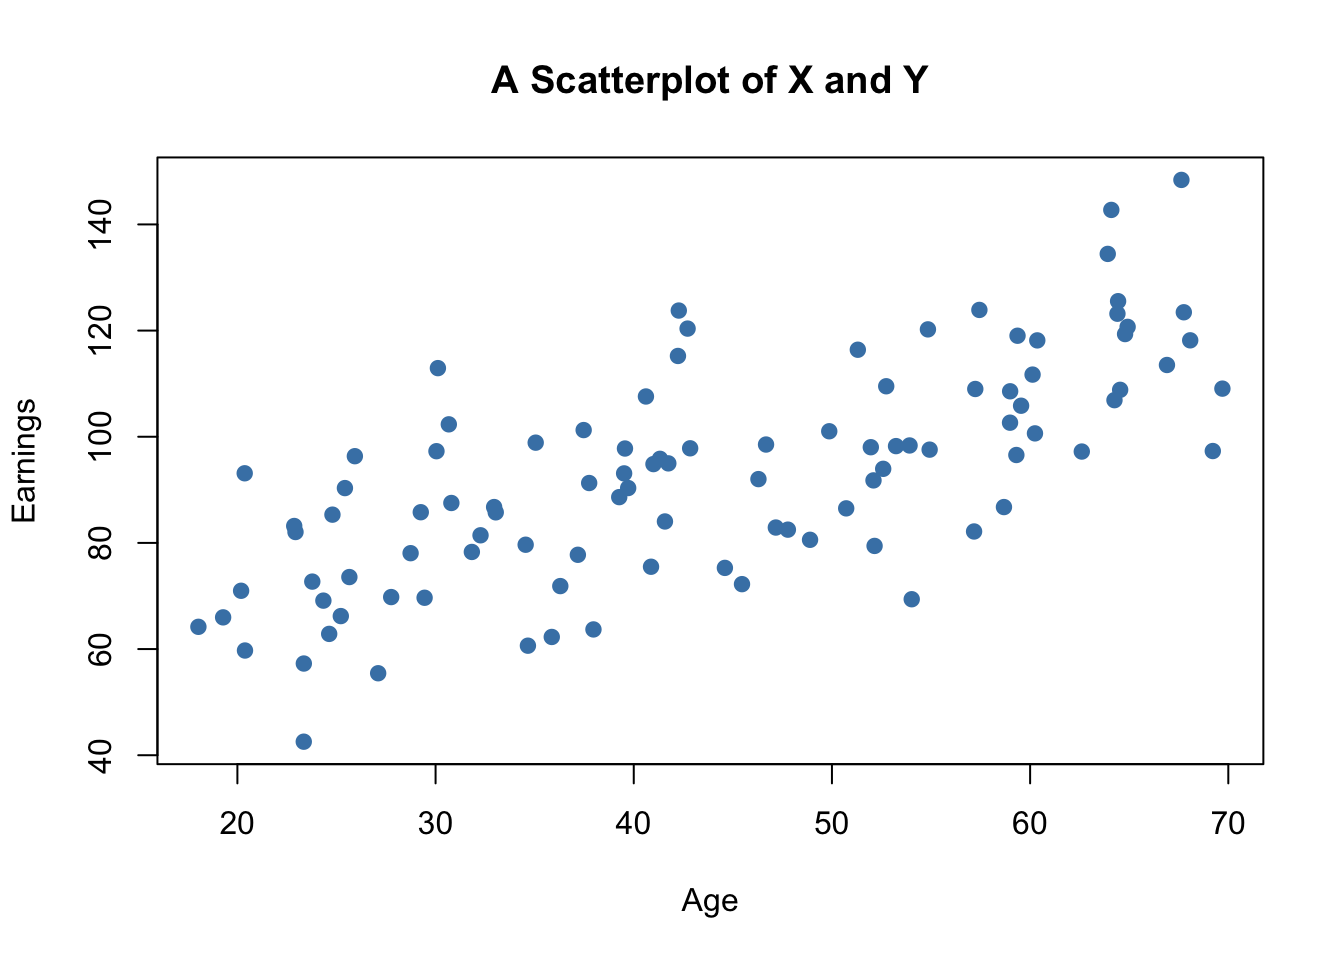
\includegraphics{ITER_files/figure-latex/unnamed-chunk-69-1} \end{center}

We see that the simulated sampling distribution of the standardized
average tends to deviate strongly from the standard normal distribution
if the sample size is small, e.g., for \(n=5\) and \(n=10\). However as
\(n\) grows, the histograms approach the standard normal distribution.
The approximation works quite well, see \(n=100\).

\section{Exercises}\label{exercises}

\begin{center}\textit{This interactive part of the book is only available in the HTML version.}\end{center}

\chapter{A Review of Statistics using R}\label{arosur}

This section reviews important statistical concepts:

\begin{itemize}
\item
  Estimation of unknown population parameters
\item
  Hypothesis testing
\item
  Confidence intervals
\end{itemize}

These methods are heavily used in econometrics. We will discuss them in
the simple context of inference about an unknown population mean and
discuss several applications in \texttt{R}. These \texttt{R}
applications rely on the following packages which are not part of the
base version of \texttt{R}:

\begin{itemize}
\item
  \texttt{readxl} - allows to import data from \emph{Excel} to
  \texttt{R}.
\item
  \texttt{dplyr} - provides a flexible grammar for data manipulation.
\item
  \texttt{MASS} - a collection of functions for applied statistics.
\end{itemize}

Make sure these are installed before you go ahead and try to replicate
the examples. The safest way to do so is by checking whether the
following code chunk executes without any errors.

\begin{Shaded}
\begin{Highlighting}[]
\KeywordTok{library}\NormalTok{(dplyr)}
\KeywordTok{library}\NormalTok{(MASS)}
\KeywordTok{library}\NormalTok{(readxl)}
\end{Highlighting}
\end{Shaded}

\section{Estimation of the Population
Mean}\label{estimation-of-the-population-mean}

\begin{keyconcepts}[Estimators and Estimates]{3.1}
\textit{Estimators} are functions of sample data that are drawn randomly from an unknown population. \textit{Estimates} are numeric values computed by estimators based on the sample data. Estimators are random variables because they are functions of \textit{random} data. Estimates are nonrandom numbers.
\end{keyconcepts}

Think of some economic variable, for example hourly earnings of college
graduates, denoted by \(Y\). Suppose we are interested in \(\mu_Y\) the
mean of \(Y\). In order to exactly calculate \(\mu_Y\) we would have to
interview every working graduate in the economy. We simply cannot do
this due to time and cost constraints. However, we can draw a random
sample of \(n\) i.i.d. observations \(Y_1, \dots, Y_n\) and estimate
\(\mu_Y\) using one of the simplest estimators in the sense of Key
Concept 3.1 one can think of, that is,

\[ \overline{Y} = \frac{1}{n} \sum_{i=1}^n Y_i, \]

the sample mean of \(Y\). Then again, we could use an even simpler
estimator for \(\mu_Y\): the very first observation in the sample,
\(Y_1\). Is \(Y_1\) a good estimator? For now, assume that

\[ Y \sim \chi_{12}^2 \]

which is not too unreasonable as hourly income is non-negative and we
expect many hourly earnings to be in a range of \(5€\,\) to \(15€\).
Moreover, it is common for income distributions to be skewed to the
right --- a property of the \(\chi^2_{12}\) distribution.

\begin{Shaded}
\begin{Highlighting}[]
\CommentTok{# plot the chi_12^2 distribution}
\KeywordTok{curve}\NormalTok{(}\KeywordTok{dchisq}\NormalTok{(x, }\DataTypeTok{df=}\DecValTok{12}\NormalTok{), }
      \DataTypeTok{from =} \DecValTok{0}\NormalTok{, }
      \DataTypeTok{to =} \DecValTok{40}\NormalTok{, }
      \DataTypeTok{ylab =} \StringTok{"density"}\NormalTok{, }
      \DataTypeTok{xlab =} \StringTok{"hourly earnings in Euro"}\NormalTok{)}
\end{Highlighting}
\end{Shaded}

\begin{center}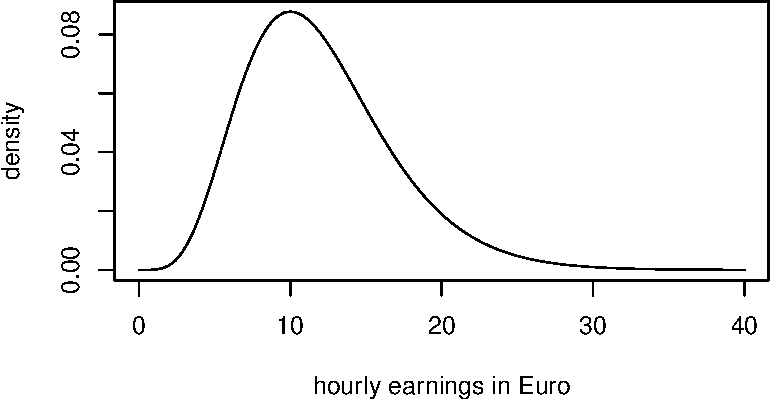
\includegraphics{ITER_files/figure-latex/unnamed-chunk-88-1} \end{center}

We now draw a sample of \(n=100\) observations and take the first
observation \(Y_1\) as an estimate for \(\mu_Y\)

\begin{Shaded}
\begin{Highlighting}[]
\CommentTok{# set seed for reproducibility}
\KeywordTok{set.seed}\NormalTok{(}\DecValTok{1}\NormalTok{)}

\CommentTok{# sample from the chi_12^2 distribution, keep only the first observation}
\KeywordTok{rchisq}\NormalTok{(}\DataTypeTok{n =} \DecValTok{100}\NormalTok{, }\DataTypeTok{df =} \DecValTok{12}\NormalTok{)[}\DecValTok{1}\NormalTok{]}
\end{Highlighting}
\end{Shaded}

\begin{verbatim}
## [1] 8.257893
\end{verbatim}

The estimate \(8.26\) is not too far away from \(\mu_Y = 12\) but it is
somewhat intuitive that we could do better: the estimator \(Y_1\)
discards a lot of information and its variance is the population
variance:

\[ \text{Var}(Y_1) = \text{Var}(Y) = 2 \cdot 12 = 24 \]

This brings us to the following question: What is a \emph{good}
estimator of an unknown parameter in the first place? This question is
tackled in Key Concepts 3.2 and 3.3.

\begin{keyconcepts}[Bias\comma Consistency and Efficiency]{3.2}
Desirable characteristics of an estimator include unbiasedness, consistency and efficiency.\newline

\textbf{Unbiasedness:}

If the mean of the sampling distribution of some estimator $\hat\mu_Y$ for the population mean $\mu_Y$ equals $\mu_Y$,
$$ E(\hat\mu_Y) = \mu_Ym, $$
the estimator is unbiased for $\mu_Y$. The \textit{bias} of $\hat\mu_Y$ then is $0$:

$$ E(\hat\mu_Y) - \mu_Y = 0$$

\textbf{Consistency:}

We want the uncertainty of the estimator $\mu_Y$ to decrease as the number of observations in the sample grows. More precisely, we want the probability that the estimate $\hat\mu_Y$ falls within a small interval around the true value $\mu_Y$ to get increasingly closer to $1$ as $n$ grows. We write this as

$$ \hat\mu_Y \xrightarrow{p} \mu_Y. $$

\textbf{Variance and efficiency:}

We want the estimator to be efficient. Suppose we have two estimators, $\hat\mu_Y$ and $\overset{\sim}{\mu}_Y$ and for some given sample size $n$ it holds that

$$ E(\hat\mu_Y) = E(\overset{\sim}{\mu}_Y) = \mu_Y $$
but
$$\text{Var}(\hat\mu_Y) < \text{Var}(\overset{\sim}{\mu}_Y).$$

We then prefer to use $\hat\mu_Y$ as it has a lower variance than $\overset{\sim}{\mu}_Y$, meaning that $\hat\mu_Y$ is more \textit{efficient} in using the information provided by the observations in the sample.
\end{keyconcepts}

\section{Properties of the Sample Mean}\label{potsm}

\BeginKnitrBlock{rmdknit}
A more precise way to express consistency of an estimator \(\hat\mu\)
for a parameter \(\mu\) is

\[ P(|\hat{\mu} - \mu|<\epsilon) \xrightarrow[n \rightarrow \infty]{p} 1 \quad \text{for any}\quad\epsilon>0.\]

This expression says that the probability of observing a deviation from
the true value \(\mu\) that is smaller than some arbitrary
\(\epsilon > 0\) converges to \(1\) as \(n\) grows. Consistency does not
require unbiasedness.
\EndKnitrBlock{rmdknit}

To examine properties of the sample mean as an estimator for the
corresponding population mean, consider the following \texttt{R}
example.

We generate a population \texttt{pop} consisting of observations
\(Y_i\), \(i=1,\dots,10000\) that origin from a normal distribution with
mean \(\mu = 10\) and variance \(\sigma^2 = 1\).

To investigate the behavior of the estimator \(\hat{\mu} = \bar{Y}\) we
can draw random samples from this population and calculate \(\bar{Y}\)
for each of them. This is easily done by making use of the function
\texttt{replicate()}. The argument \texttt{expr} is evaluated \texttt{n}
times. In this case we draw samples of sizes \(n=5\) and \(n=25\),
compute the sample means and repeat this exactly \(N=25000\) times.

For comparison purposes we store results for the estimator \(Y_1\), the
first observation in a sample for a sample of size \(5\), separately.

\begin{Shaded}
\begin{Highlighting}[]
\CommentTok{# generate a fictious population}
\NormalTok{pop <-}\StringTok{ }\KeywordTok{rnorm}\NormalTok{(}\DecValTok{10000}\NormalTok{, }\DecValTok{10}\NormalTok{, }\DecValTok{1}\NormalTok{)}

\CommentTok{# sample from the population and estimate the mean}
\NormalTok{est1 <-}\StringTok{ }\KeywordTok{replicate}\NormalTok{(}\DataTypeTok{expr =} \KeywordTok{mean}\NormalTok{(}\KeywordTok{sample}\NormalTok{(}\DataTypeTok{x =}\NormalTok{ pop, }\DataTypeTok{size =} \DecValTok{5}\NormalTok{)), }\DataTypeTok{n =} \DecValTok{25000}\NormalTok{)}

\NormalTok{est2 <-}\StringTok{ }\KeywordTok{replicate}\NormalTok{(}\DataTypeTok{expr =} \KeywordTok{mean}\NormalTok{(}\KeywordTok{sample}\NormalTok{(}\DataTypeTok{x =}\NormalTok{ pop, }\DataTypeTok{size =} \DecValTok{25}\NormalTok{)), }\DataTypeTok{n =} \DecValTok{25000}\NormalTok{)}

\NormalTok{fo <-}\StringTok{ }\KeywordTok{replicate}\NormalTok{(}\DataTypeTok{expr =} \KeywordTok{sample}\NormalTok{(}\DataTypeTok{x =}\NormalTok{ pop, }\DataTypeTok{size =} \DecValTok{5}\NormalTok{)[}\DecValTok{1}\NormalTok{], }\DataTypeTok{n =} \DecValTok{25000}\NormalTok{)}
\end{Highlighting}
\end{Shaded}

Check that \texttt{est1} and \texttt{est2} are vectors of length
\(25000\):

\begin{Shaded}
\begin{Highlighting}[]
\CommentTok{# check if object type is vector}
\KeywordTok{is.vector}\NormalTok{(est1)}
\end{Highlighting}
\end{Shaded}

\begin{verbatim}
## [1] TRUE
\end{verbatim}

\begin{Shaded}
\begin{Highlighting}[]
\KeywordTok{is.vector}\NormalTok{(est2)}
\end{Highlighting}
\end{Shaded}

\begin{verbatim}
## [1] TRUE
\end{verbatim}

\begin{Shaded}
\begin{Highlighting}[]
\CommentTok{# check length}
\KeywordTok{length}\NormalTok{(est1)}
\end{Highlighting}
\end{Shaded}

\begin{verbatim}
## [1] 25000
\end{verbatim}

\begin{Shaded}
\begin{Highlighting}[]
\KeywordTok{length}\NormalTok{(est2)}
\end{Highlighting}
\end{Shaded}

\begin{verbatim}
## [1] 25000
\end{verbatim}

The code chunk below produces a plot of the sampling distributions of
the estimators \(\bar{Y}\) and \(Y_1\) on the basis of the \(25000\)
samples in each case. We also plot the density function of the
\(\mathcal{N}(10,1)\) distribution.

\begin{Shaded}
\begin{Highlighting}[]
\CommentTok{# plot density estimate Y_1}
\KeywordTok{plot}\NormalTok{(}\KeywordTok{density}\NormalTok{(fo), }
      \DataTypeTok{col =} \StringTok{'green'}\NormalTok{, }
      \DataTypeTok{lwd =} \DecValTok{2}\NormalTok{,}
      \DataTypeTok{ylim =} \KeywordTok{c}\NormalTok{(}\DecValTok{0}\NormalTok{, }\DecValTok{2}\NormalTok{),}
      \DataTypeTok{xlab =} \StringTok{'estimates'}\NormalTok{,}
      \DataTypeTok{main =} \StringTok{'Sampling Distributions of Unbiased Estimators'}\NormalTok{)}

\CommentTok{# add density estimate for the distribution of the sample mean with n=5 to the plot}
\KeywordTok{lines}\NormalTok{(}\KeywordTok{density}\NormalTok{(est1), }
     \DataTypeTok{col =} \StringTok{'steelblue'}\NormalTok{, }
     \DataTypeTok{lwd =} \DecValTok{2}\NormalTok{, }
     \DataTypeTok{bty =} \StringTok{'l'}\NormalTok{)}

\CommentTok{# add density estimate for the distribution of the sample mean with n=25 to the plot}
\KeywordTok{lines}\NormalTok{(}\KeywordTok{density}\NormalTok{(est2), }
      \DataTypeTok{col =} \StringTok{'red2'}\NormalTok{, }
      \DataTypeTok{lwd =} \DecValTok{2}\NormalTok{)}

\CommentTok{# add a vertical line at the true parameter}
\KeywordTok{abline}\NormalTok{(}\DataTypeTok{v =} \DecValTok{10}\NormalTok{, }\DataTypeTok{lty =} \DecValTok{2}\NormalTok{)}

\CommentTok{# add N(10,1) density to the plot}
\KeywordTok{curve}\NormalTok{(}\KeywordTok{dnorm}\NormalTok{(x, }\DataTypeTok{mean =} \DecValTok{10}\NormalTok{), }
     \DataTypeTok{lwd =} \DecValTok{2}\NormalTok{,}
     \DataTypeTok{lty =} \DecValTok{2}\NormalTok{,}
     \DataTypeTok{add =}\NormalTok{ T)}

\CommentTok{# add a legend}
\KeywordTok{legend}\NormalTok{(}\StringTok{"topleft"}\NormalTok{,}
       \DataTypeTok{legend =} \KeywordTok{c}\NormalTok{(}\StringTok{"N(10,1)"}\NormalTok{,}
                  \KeywordTok{expression}\NormalTok{(Y[}\DecValTok{1}\NormalTok{]),}
                  \KeywordTok{expression}\NormalTok{(}\KeywordTok{bar}\NormalTok{(Y) }\OperatorTok{~}\StringTok{ }\NormalTok{n }\OperatorTok{==}\StringTok{ }\DecValTok{5}\NormalTok{),}
                  \KeywordTok{expression}\NormalTok{(}\KeywordTok{bar}\NormalTok{(Y) }\OperatorTok{~}\StringTok{ }\NormalTok{n }\OperatorTok{==}\StringTok{ }\DecValTok{25}\NormalTok{)}
\NormalTok{                  ), }
       \DataTypeTok{lty =} \KeywordTok{c}\NormalTok{(}\DecValTok{2}\NormalTok{, }\DecValTok{1}\NormalTok{, }\DecValTok{1}\NormalTok{, }\DecValTok{1}\NormalTok{), }
       \DataTypeTok{col =} \KeywordTok{c}\NormalTok{(}\StringTok{'black'}\NormalTok{,}\StringTok{'green'}\NormalTok{, }\StringTok{'steelblue'}\NormalTok{, }\StringTok{'red2'}\NormalTok{),}
       \DataTypeTok{lwd =} \DecValTok{2}\NormalTok{)}
\end{Highlighting}
\end{Shaded}

\begin{center}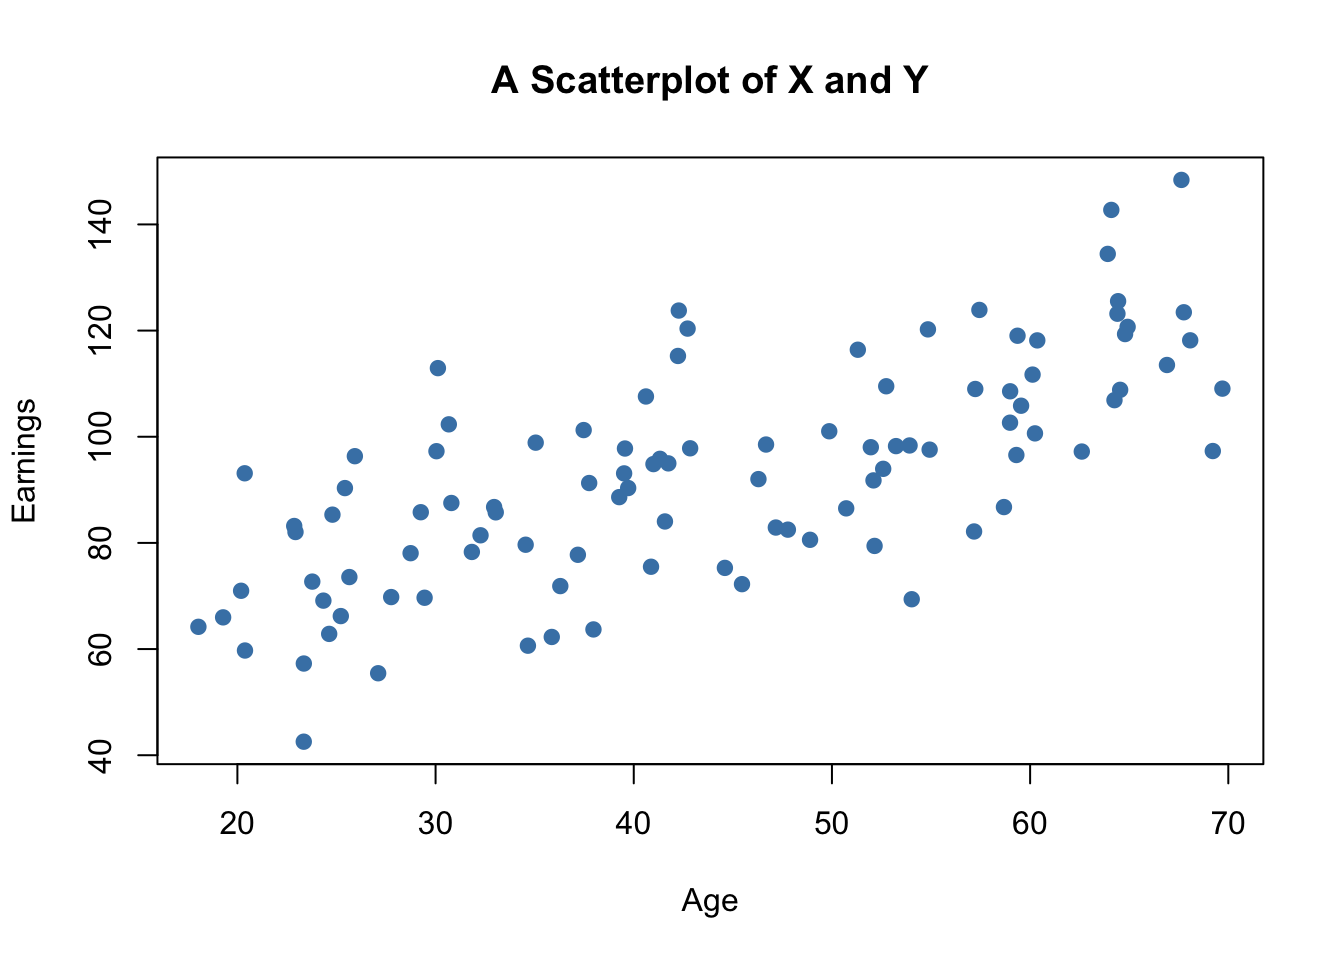
\includegraphics{ITER_files/figure-latex/unnamed-chunk-94-1} \end{center}

First, \emph{all} sampling distributions (represented by the solid
lines) are centered around \(\mu = 10\). This is evidence for the
\emph{unbiasedness} of \(Y_1\), \(\overline{Y}_{5}\) and
\(\overline{Y}_{25}\). Of course, the theoretical density
\(\mathcal{N}(10,1)\) is centered at \(10\), too.

Next, have a look at the spread of the sampling distributions. Several
things are noteworthy:

\begin{itemize}
\item
  The sampling distribution of \(Y_1\) (green curve) tracks the density
  of the \(\mathcal{N}(10,1)\) distribution (black dashed line) pretty
  closely. In fact, the sampling distribution of \(Y_1\) is the
  \(\mathcal{N}(10,1)\) distribution. This is less surprising if you
  keep in mind that the \(Y_1\) estimator does nothing but reporting an
  observation that is randomly selected from a population with
  \(\mathcal{N}(10,1)\) distribution. Hence,
  \(Y_1 \sim \mathcal{N}(10,1)\). Note that this result does not depend
  on the sample size \(n\): the sampling distribution of \(Y_1\)
  \emph{is always} the population distribution, no matter how large the
  sample is. \(Y_1\) is a good a estimate of \(\mu_Y\), but we can do
  better.
\item
  Both sampling distributions of \(\overline{Y}\) show less dispersion
  than the sampling distribution of \(Y_1\). This means that
  \(\overline{Y}\) has a lower variance than \(Y_1\). In view of Key
  Concepts 3.2 and 3.3, we find that \(\overline{Y}\) is a more
  efficient estimator than \(Y_1\). In fact, this holds for all \(n>1\).
\item
  \(\overline{Y}\) shows a behavior illustrating consistency (see Key
  Concept 3.2). The blue and the red densities are much more
  concentrated around \(\mu=10\) than the green one. As the number of
  observations is increased from \(1\) to \(5\), the sampling
  distribution tightens around the true parameter. Increasing the sample
  size to \(25\), this effect becomes more apparent. This implies that
  the probability of obtaining estimates that are close to the true
  value increases with \(n\).
\end{itemize}

We encourage you to go ahead and modify the code. Try out different
values for the sample size and see how the sampling distribution of
\(\overline{Y}\) changes!

\subsubsection*{\texorpdfstring{\(\overline{Y}\) is the Least Squares
Estimator of
\(\mu_Y\)}{\textbackslash{}overline\{Y\} is the Least Squares Estimator of \textbackslash{}mu\_Y}}\label{overliney-is-the-least-squares-estimator-of-mu_y}
\addcontentsline{toc}{subsubsection}{\(\overline{Y}\) is the Least
Squares Estimator of \(\mu_Y\)}

Assume you have some observations \(Y_1,\dots,Y_n\) on
\(Y \sim \mathcal{N}(10,1)\) (which is unknown) and would like to find
an estimator \(m\) that predicts the observations as well as possible.
By good we mean to choose \(m\) such that the total squared deviation
between the predicted value and the observed values is small.
Mathematically, this means we want to find an \(m\) that minimizes

\begin{equation}
  \sum_{i=1}^n (Y_i - m)^2. \label{eq:sqm}
\end{equation}

Think of \(Y_i - m\) as the mistake made when predicting \(Y_i\) by
\(m\). We could also minimize the sum of absolute deviations from \(m\)
but minimizing the sum of squared deviations is mathematically more
convenient (and will lead to a different result). That is why the
estimator we are looking for is called the \emph{least squares
estimator}. \(m = \overline{Y}\), the sample mean, is this estimator.

We can show this by generating a random sample and plotting \eqref{eq:sqm}
as a function of \(m\).

\begin{Shaded}
\begin{Highlighting}[]
\CommentTok{# define the function and vectorize it}
\NormalTok{sqm <-}\StringTok{ }\ControlFlowTok{function}\NormalTok{(m) \{}
 \KeywordTok{sum}\NormalTok{((y}\OperatorTok{-}\NormalTok{m)}\OperatorTok{^}\DecValTok{2}\NormalTok{)}
\NormalTok{\}}
\NormalTok{sqm <-}\StringTok{ }\KeywordTok{Vectorize}\NormalTok{(sqm)}

\CommentTok{# draw random sample and compute the mean}
\NormalTok{y <-}\StringTok{ }\KeywordTok{rnorm}\NormalTok{(}\DecValTok{100}\NormalTok{, }\DecValTok{10}\NormalTok{, }\DecValTok{1}\NormalTok{)}
\KeywordTok{mean}\NormalTok{(y)}
\end{Highlighting}
\end{Shaded}

\begin{verbatim}
## [1] 10.00543
\end{verbatim}

\begin{Shaded}
\begin{Highlighting}[]
\CommentTok{# plot the objective function}
\KeywordTok{curve}\NormalTok{(}\KeywordTok{sqm}\NormalTok{(x), }
      \DataTypeTok{from =} \OperatorTok{-}\DecValTok{50}\NormalTok{, }
      \DataTypeTok{to =} \DecValTok{70}\NormalTok{,}
      \DataTypeTok{xlab =} \StringTok{"m"}\NormalTok{,}
      \DataTypeTok{ylab =} \StringTok{"sqm(m)"}\NormalTok{)}

\CommentTok{# add vertical line at mean(y)}
\KeywordTok{abline}\NormalTok{(}\DataTypeTok{v =} \KeywordTok{mean}\NormalTok{(y), }
       \DataTypeTok{lty =} \DecValTok{2}\NormalTok{, }
       \DataTypeTok{col =} \StringTok{"darkred"}\NormalTok{)}

\CommentTok{# add annotation at mean(y)}
\KeywordTok{text}\NormalTok{(}\DataTypeTok{x =} \KeywordTok{mean}\NormalTok{(y), }
     \DataTypeTok{y =} \DecValTok{0}\NormalTok{, }
     \DataTypeTok{labels =} \KeywordTok{paste}\NormalTok{(}\KeywordTok{round}\NormalTok{(}\KeywordTok{mean}\NormalTok{(y), }\DecValTok{2}\NormalTok{)))}
\end{Highlighting}
\end{Shaded}

\begin{center}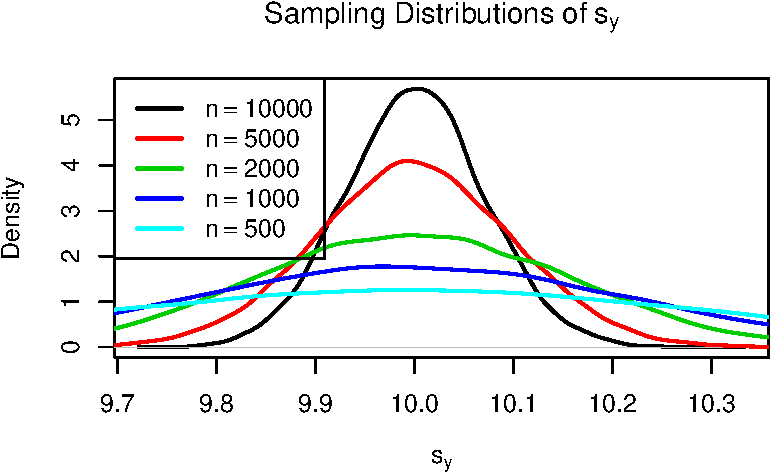
\includegraphics{ITER_files/figure-latex/unnamed-chunk-96-1} \end{center}

Notice that \eqref{eq:sqm} is a quadratic function so that there is only
one minimum. The plot shows that this minimum lies exactly at the sample
mean of the sample data.

\BeginKnitrBlock{rmdknit}
Some R functions can only interact with functions that take a vector as
an input and evaluate the function body on every entry of the vector,
for example curve(). We call such functions vectorized functions and it
is often a good idea to write vectorized functions yourself, although
this is cumbersome in some cases. Having a vectorized function in R is
never a drawback since these functions work on both single values and
vectors.

Let us look at the function sqm(), which is non-vectorized:

 sqm \textless{}- function(m) \{\\
\hspace*{0.333em}\hspace*{0.333em}\hspace*{0.333em}\hspace*{0.333em}
sum((y-m)\^{}2) \#body of the function\\
\}

Providing, e.g., c(1,2,3) as the argument m would cause an error since
then the operation y-m is invalid: the vectors y and m are of
incompatible dimensions. This is why we cannot use sqm() in conjunction
with curve().

Here Vectorize() comes into play. It generates a vectorized version of a
non-vectorized function.
\EndKnitrBlock{rmdknit}

\subsubsection*{Why Random Sampling is
Important}\label{why-random-sampling-is-important}
\addcontentsline{toc}{subsubsection}{Why Random Sampling is Important}

So far, we assumed (sometimes implicitly) that the observed data
\(Y_1, \dots, Y_n\) are the result of a sampling process that satisfies
the assumption of simple random sampling. This assumption often is
fulfilled when estimating a population mean using \(\overline{Y}\). If
this is not the case, estimates may be biased.

Let us fall back to \texttt{pop}, the fictive population of \(10000\)
observations and compute the population mean \(\mu_{\texttt{pop}}\):

\begin{Shaded}
\begin{Highlighting}[]
\CommentTok{# compute the population mean of pop}
\KeywordTok{mean}\NormalTok{(pop)}
\end{Highlighting}
\end{Shaded}

\begin{verbatim}
## [1] 9.992604
\end{verbatim}

Next we sample \(10\) observations from \texttt{pop} with
\texttt{sample()} and estimate \(\mu_{\texttt{pop}}\) using
\(\overline{Y}\) repeatedly. However, now we use a sampling scheme that
deviates from simple random sampling: instead of ensuring that each
member of the population has the same chance to end up in a sample, we
assign a higher probability of being sampled to the \(2500\) smallest
observations of the population by setting the argument \texttt{prop} to
a suitable vector of probability weights:

\begin{Shaded}
\begin{Highlighting}[]
\CommentTok{# simulate outcomes for the sample mean when the i.i.d. assumption fails}
\NormalTok{est3 <-}\StringTok{  }\KeywordTok{replicate}\NormalTok{(}\DataTypeTok{n =} \DecValTok{25000}\NormalTok{, }
                   \DataTypeTok{expr =} \KeywordTok{mean}\NormalTok{(}\KeywordTok{sample}\NormalTok{(}\DataTypeTok{x =} \KeywordTok{sort}\NormalTok{(pop), }
                                      \DataTypeTok{size =} \DecValTok{10}\NormalTok{, }
                                      \DataTypeTok{prob =} \KeywordTok{c}\NormalTok{(}\KeywordTok{rep}\NormalTok{(}\DecValTok{4}\NormalTok{, }\DecValTok{2500}\NormalTok{), }\KeywordTok{rep}\NormalTok{(}\DecValTok{1}\NormalTok{, }\DecValTok{7500}\NormalTok{)))))}

\CommentTok{# compute the sample mean of the outcomes}
\KeywordTok{mean}\NormalTok{(est3)}
\end{Highlighting}
\end{Shaded}

\begin{verbatim}
## [1] 9.443454
\end{verbatim}

Next we plot the sampling distribution of \(\overline{Y}\) for this
non-i.i.d. case and compare it to the sampling distribution when the
i.i.d. assumption holds.

\begin{Shaded}
\begin{Highlighting}[]
\CommentTok{# sampling distribution of sample mean, i.i.d. holds, n=25}
\KeywordTok{plot}\NormalTok{(}\KeywordTok{density}\NormalTok{(est2), }
      \DataTypeTok{col =} \StringTok{'steelblue'}\NormalTok{,}
      \DataTypeTok{lwd =} \DecValTok{2}\NormalTok{,}
      \DataTypeTok{xlim =} \KeywordTok{c}\NormalTok{(}\DecValTok{8}\NormalTok{, }\DecValTok{11}\NormalTok{),}
      \DataTypeTok{xlab =} \StringTok{'Estimates'}\NormalTok{,}
      \DataTypeTok{main =} \StringTok{'When the i.i.d. Assumption Fails'}\NormalTok{)}

\CommentTok{# sampling distribution of sample mean, i.i.d. fails, n=25}
\KeywordTok{lines}\NormalTok{(}\KeywordTok{density}\NormalTok{(est3),}
      \DataTypeTok{col =} \StringTok{'red2'}\NormalTok{,}
      \DataTypeTok{lwd =} \DecValTok{2}\NormalTok{)}

\CommentTok{# add a legend}
\KeywordTok{legend}\NormalTok{(}\StringTok{"topleft"}\NormalTok{,}
       \DataTypeTok{legend =} \KeywordTok{c}\NormalTok{(}\KeywordTok{expression}\NormalTok{(}\KeywordTok{bar}\NormalTok{(Y)[n }\OperatorTok{==}\StringTok{ }\DecValTok{25}\NormalTok{]}\OperatorTok{~}\StringTok{", i.i.d. fails"}\NormalTok{),}
                  \KeywordTok{expression}\NormalTok{(}\KeywordTok{bar}\NormalTok{(Y)[n }\OperatorTok{==}\StringTok{ }\DecValTok{25}\NormalTok{]}\OperatorTok{~}\StringTok{", i.i.d. holds"}\NormalTok{)}
\NormalTok{                  ), }
       \DataTypeTok{lty =} \KeywordTok{c}\NormalTok{(}\DecValTok{1}\NormalTok{, }\DecValTok{1}\NormalTok{), }
       \DataTypeTok{col =} \KeywordTok{c}\NormalTok{(}\StringTok{'red2'}\NormalTok{, }\StringTok{'steelblue'}\NormalTok{),}
       \DataTypeTok{lwd =} \DecValTok{2}\NormalTok{)}
\end{Highlighting}
\end{Shaded}

\begin{center}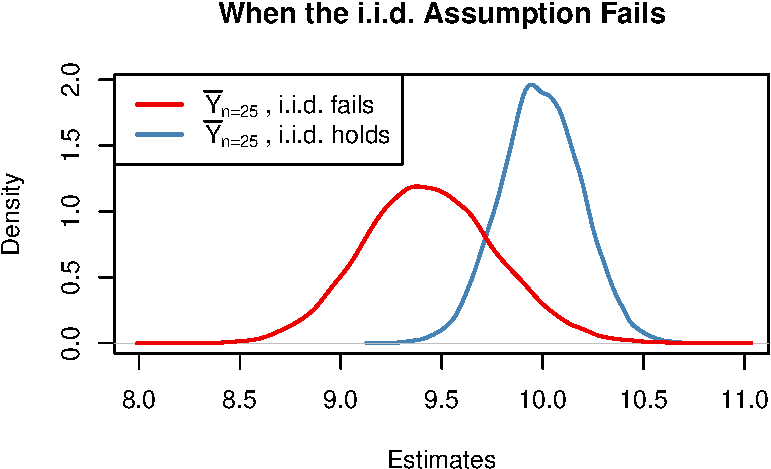
\includegraphics{ITER_files/figure-latex/unnamed-chunk-99-1} \end{center}

Here, the failure of the i.i.d. assumption implies that, on average, we
\emph{underestimate} \(\mu_Y\) using \(\overline{Y}\): the corresponding
distribution of \(\overline{Y}\) is shifted to the left. In other words,
\(\overline{Y}\) is a \emph{biased} estimator for \(\mu_Y\) if the
i.i.d. assumption does not hold.

\section{Hypothesis Tests Concerning the Population
Mean}\label{hypothesis-tests-concerning-the-population-mean}

In this section we briefly review concepts in hypothesis testing and
discuss how to conduct hypothesis tests in \texttt{R}. We focus on
drawing inferences about an unknown population mean.

\subsubsection*{About Hypotheses and Hypothesis
Testing}\label{about-hypotheses-and-hypothesis-testing}
\addcontentsline{toc}{subsubsection}{About Hypotheses and Hypothesis
Testing}

In a significance test we want to exploit the information contained in a
sample as evidence in favor or against a hypothesis. Essentially,
hypotheses are simple questions that can be answered by `yes' or `no'.
In a hypothesis test we typically deal with two different hypotheses:

\begin{itemize}
\item
  The \emph{null hypothesis}, denoted \(H_0\), is the hypothesis we are
  interested in testing.
\item
  There must be an \emph{alternative hypothesis}, denoted \(H_1\), the
  hypothesis that is thought to hold if the null hypothesis is rejected.
\end{itemize}

The null hypothesis that the population mean of \(Y\) equals the value
\(\mu_{Y,0}\) is written as

\[ H_0: E(Y) = \mu_{Y,0}. \]

Often the alternative hypothesis chosen is the most general one,

\[ H_1: E(Y) \neq \mu_{Y,0}, \]

meaning that \(E(Y)\) may be anything but the value under the null
hypothesis. This is called a \emph{two-sided} alternative.

For the sake of brevity, we only consider two-sided alternatives in the
subsequent sections of this chapter.

\subsection*{The p-Value}\label{the-p-value}
\addcontentsline{toc}{subsection}{The p-Value}

Assume that the null hypothesis is \emph{true}. The \(p\)-value is the
probability of drawing data and observing a corresponding test statistic
that is at least as adverse to what is stated under the null hypothesis
as the test statistic actually computed using the sample data.

In the context of the population mean and the sample mean, this
definition can be stated mathematically in the following way:

\begin{equation}
p \text{-value} = P_{H_0}\left[ \lvert \overline{Y} - \mu_{Y,0} \rvert > \lvert \overline{Y}^{act} - \mu_{Y,0} \rvert \right] \label{eq:pvalue}
\end{equation}

In \eqref{eq:pvalue}, \(\overline{Y}^{act}\) is the mean of the sample
actually computed. Consequently, in order to compute the \(p\)-value as
in \eqref{eq:pvalue}, knowledge about the sampling distribution of
\(\overline{Y}\) when the null hypothesis is true is required. However
in most cases the sampling distribution of \(\overline{Y}\) is unknown.
Fortunately, as stated by the CLT (see Key Concept 2.7), the
large-sample approximation
\[ \overline{Y} \approx \mathcal{N}(\mu_{Y,0}, \, \sigma^2_{\overline{Y}}) \ \ , \ \ \sigma^2_{\overline{Y}} = \frac{\sigma_Y^2}{n} \]

can be made under the null. Thus,

\[ \frac{\overline{Y} - \mu_{Y,0}}{\sigma_Y/\sqrt{n}} \sim \mathcal{N}(0,1). \]

So in large samples, the \(p\)-value can be computed \emph{without}
knowledge of the exact sampling distribution of \(\overline{Y}\).

\subsection*{Calculating the p-Value when the Standard Deviation is
Known}\label{calculating-the-p-value-when-the-standard-deviation-is-known}
\addcontentsline{toc}{subsection}{Calculating the p-Value when the
Standard Deviation is Known}

For now, let us assume that \(\sigma_{\overline{Y}}\) is known. Then, we
can rewrite \eqref{eq:pvalue} as

\begin{align}
p \text{-value} =& \, P_{H_0}\left[ \left\lvert \frac{\overline{Y} - \mu_{Y,0}}{\sigma_{\overline{Y}}} \right\rvert > \left\lvert \frac{\overline{Y}^{act} - \mu_{Y,0}}{\sigma_{\overline{Y}}} \right\rvert \right] \\
=& \, 2 \cdot \Phi \left[ - \left\lvert \frac{\overline{Y}^{act} - \mu_{Y,0}}{\sigma_{\overline{Y}}}  \right\rvert\right].  \label{eq:pvaluenorm1}
\end{align}

The \(p\)-value can be seen as the area in the tails of the
\(\mathcal{N}(0,1)\) distribution that lies beyond

\begin{equation}
\pm \left\lvert \frac{\overline{Y}^{act} - \mu_{Y,0}}{\sigma_{\overline{Y}}} \right\rvert \label{eq:pvaluenorm2}
\end{equation}

We now use \texttt{R} to visualize what is stated in
\eqref{eq:pvaluenorm1} and \eqref{eq:pvaluenorm2}. The next code chunk
replicates Figure 3.1 of the book.

\begin{Shaded}
\begin{Highlighting}[]
\CommentTok{# plot the standard normal density on the interval [-4,4]}
\KeywordTok{curve}\NormalTok{(}\KeywordTok{dnorm}\NormalTok{(x),}
      \DataTypeTok{xlim =} \KeywordTok{c}\NormalTok{(}\OperatorTok{-}\DecValTok{4}\NormalTok{, }\DecValTok{4}\NormalTok{),}
      \DataTypeTok{main =} \StringTok{'Calculating a p-Value'}\NormalTok{,}
      \DataTypeTok{yaxs =} \StringTok{'i'}\NormalTok{,}
      \DataTypeTok{xlab =} \StringTok{'z'}\NormalTok{,}
      \DataTypeTok{ylab =} \StringTok{''}\NormalTok{,}
      \DataTypeTok{lwd =} \DecValTok{2}\NormalTok{,}
      \DataTypeTok{axes =} \StringTok{'F'}\NormalTok{)}

\CommentTok{# add x-axis}
\KeywordTok{axis}\NormalTok{(}\DecValTok{1}\NormalTok{, }
     \DataTypeTok{at =} \KeywordTok{c}\NormalTok{(}\OperatorTok{-}\FloatTok{1.5}\NormalTok{, }\DecValTok{0}\NormalTok{, }\FloatTok{1.5}\NormalTok{), }
     \DataTypeTok{padj =} \FloatTok{0.75}\NormalTok{,}
     \DataTypeTok{labels =} \KeywordTok{c}\NormalTok{(}\KeywordTok{expression}\NormalTok{(}\OperatorTok{-}\KeywordTok{frac}\NormalTok{(}\KeywordTok{bar}\NormalTok{(Y)}\OperatorTok{^}\StringTok{"act"}\OperatorTok{~-}\ErrorTok{~}\KeywordTok{bar}\NormalTok{(mu)[Y,}\DecValTok{0}\NormalTok{], sigma[}\KeywordTok{bar}\NormalTok{(Y)])),}
                \DecValTok{0}\NormalTok{,}
                \KeywordTok{expression}\NormalTok{(}\KeywordTok{frac}\NormalTok{(}\KeywordTok{bar}\NormalTok{(Y)}\OperatorTok{^}\StringTok{"act"}\OperatorTok{~-}\ErrorTok{~}\KeywordTok{bar}\NormalTok{(mu)[Y,}\DecValTok{0}\NormalTok{], sigma[}\KeywordTok{bar}\NormalTok{(Y)]))))}

\CommentTok{# shade p-value/2 region in left tail}
\KeywordTok{polygon}\NormalTok{(}\DataTypeTok{x =} \KeywordTok{c}\NormalTok{(}\OperatorTok{-}\DecValTok{6}\NormalTok{, }\KeywordTok{seq}\NormalTok{(}\OperatorTok{-}\DecValTok{6}\NormalTok{, }\OperatorTok{-}\FloatTok{1.5}\NormalTok{, }\FloatTok{0.01}\NormalTok{), }\OperatorTok{-}\FloatTok{1.5}\NormalTok{),}
        \DataTypeTok{y =} \KeywordTok{c}\NormalTok{(}\DecValTok{0}\NormalTok{, }\KeywordTok{dnorm}\NormalTok{(}\KeywordTok{seq}\NormalTok{(}\OperatorTok{-}\DecValTok{6}\NormalTok{, }\OperatorTok{-}\FloatTok{1.5}\NormalTok{, }\FloatTok{0.01}\NormalTok{)),}\DecValTok{0}\NormalTok{), }
        \DataTypeTok{col =} \StringTok{'steelblue'}\NormalTok{)}

\CommentTok{# shade p-value/2 region in right tail}
\KeywordTok{polygon}\NormalTok{(}\DataTypeTok{x =} \KeywordTok{c}\NormalTok{(}\FloatTok{1.5}\NormalTok{, }\KeywordTok{seq}\NormalTok{(}\FloatTok{1.5}\NormalTok{, }\DecValTok{6}\NormalTok{, }\FloatTok{0.01}\NormalTok{), }\DecValTok{6}\NormalTok{),}
        \DataTypeTok{y =} \KeywordTok{c}\NormalTok{(}\DecValTok{0}\NormalTok{, }\KeywordTok{dnorm}\NormalTok{(}\KeywordTok{seq}\NormalTok{(}\FloatTok{1.5}\NormalTok{, }\DecValTok{6}\NormalTok{, }\FloatTok{0.01}\NormalTok{)), }\DecValTok{0}\NormalTok{), }
        \DataTypeTok{col =} \StringTok{'steelblue'}\NormalTok{)}
\end{Highlighting}
\end{Shaded}

\begin{center}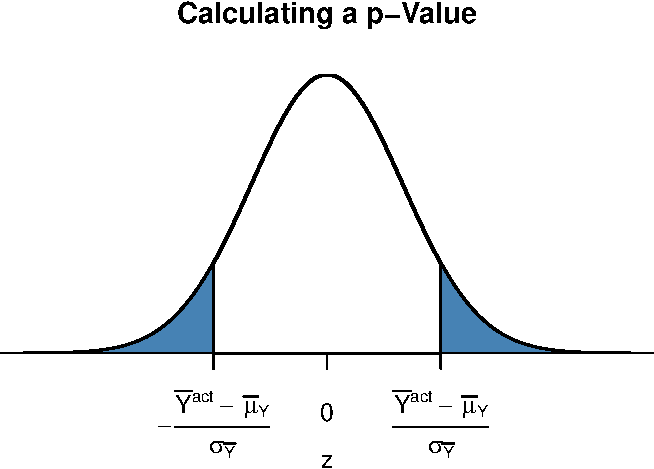
\includegraphics{ITER_files/figure-latex/unnamed-chunk-100-1} \end{center}

\hypertarget{SVSSDASE}{\subsection*{Sample Variance, Sample Standard
Deviation and Standard Error}\label{SVSSDASE}}
\addcontentsline{toc}{subsection}{Sample Variance, Sample Standard
Deviation and Standard Error}

If \(\sigma^2_Y\) is unknown, it must be estimated. This can be done
using the sample variance

\begin{equation}
s_Y^2 = \frac{1}{n-1} \sum_{i=1}^n (Y_i - \overline{Y})^2.
\end{equation}

Furthermore

\begin{equation}
s_Y = \sqrt{\frac{1}{n-1} \sum_{i=1}^n (Y_i - \overline{Y})^2}
\end{equation}

is a suitable estimator for the standard deviation of \(Y\). In
\texttt{R}, \(s_Y\) is implemented in the function \texttt{sd()}, see
\texttt{?sd}.

Using \texttt{R} we can illustrate that \(s_Y\) is a consistent
estimator for \(\sigma_Y\) with

\[ s_Y \overset{p}{\longrightarrow} \sigma_Y. \]

The idea here is to generate a large number of samples \(Y_1,\dots,Y_n\)
where, \(Y\sim \mathcal{N}(10,10)\) say, estimate \(\sigma_Y\) using
\(s_Y\) and investigate how the distribution of \(s_Y\) changes as \(n\)
gets larger.

\begin{Shaded}
\begin{Highlighting}[]
\CommentTok{# vector of sample sizes}
\NormalTok{n <-}\StringTok{ }\KeywordTok{c}\NormalTok{(}\DecValTok{10000}\NormalTok{, }\DecValTok{5000}\NormalTok{, }\DecValTok{2000}\NormalTok{, }\DecValTok{1000}\NormalTok{, }\DecValTok{500}\NormalTok{)}

\CommentTok{# sample observations, estimate using 'sd()' and plot the estimated distributions}
\NormalTok{sq_y <-}\StringTok{ }\KeywordTok{replicate}\NormalTok{(}\DataTypeTok{n =} \DecValTok{10000}\NormalTok{, }\DataTypeTok{expr =} \KeywordTok{sd}\NormalTok{(}\KeywordTok{rnorm}\NormalTok{(n[}\DecValTok{1}\NormalTok{], }\DecValTok{10}\NormalTok{, }\DecValTok{10}\NormalTok{)))}
\KeywordTok{plot}\NormalTok{(}\KeywordTok{density}\NormalTok{(sq_y),}
     \DataTypeTok{main =} \KeywordTok{expression}\NormalTok{(}\StringTok{'Sampling Distributions of'} \OperatorTok{~}\StringTok{ }\NormalTok{s[Y]),}
     \DataTypeTok{xlab =} \KeywordTok{expression}\NormalTok{(s[y]),}
     \DataTypeTok{lwd =} \DecValTok{2}\NormalTok{)}

\ControlFlowTok{for}\NormalTok{ (i }\ControlFlowTok{in} \DecValTok{2}\OperatorTok{:}\KeywordTok{length}\NormalTok{(n)) \{}
\NormalTok{  sq_y <-}\StringTok{ }\KeywordTok{replicate}\NormalTok{(}\DataTypeTok{n =} \DecValTok{10000}\NormalTok{, }\DataTypeTok{expr =} \KeywordTok{sd}\NormalTok{(}\KeywordTok{rnorm}\NormalTok{(n[i], }\DecValTok{10}\NormalTok{, }\DecValTok{10}\NormalTok{)))}
  \KeywordTok{lines}\NormalTok{(}\KeywordTok{density}\NormalTok{(sq_y), }
        \DataTypeTok{col =}\NormalTok{ i, }
        \DataTypeTok{lwd =} \DecValTok{2}\NormalTok{)}
\NormalTok{\}}

\CommentTok{# add a legend}
\KeywordTok{legend}\NormalTok{(}\StringTok{"topleft"}\NormalTok{,}
       \DataTypeTok{legend =} \KeywordTok{c}\NormalTok{(}\KeywordTok{expression}\NormalTok{(n }\OperatorTok{==}\StringTok{ }\DecValTok{10000}\NormalTok{),}
                  \KeywordTok{expression}\NormalTok{(n }\OperatorTok{==}\StringTok{ }\DecValTok{5000}\NormalTok{),}
                  \KeywordTok{expression}\NormalTok{(n }\OperatorTok{==}\StringTok{ }\DecValTok{2000}\NormalTok{),}
                  \KeywordTok{expression}\NormalTok{(n }\OperatorTok{==}\StringTok{ }\DecValTok{1000}\NormalTok{),}
                  \KeywordTok{expression}\NormalTok{(n }\OperatorTok{==}\StringTok{ }\DecValTok{500}\NormalTok{)), }
       \DataTypeTok{col =} \DecValTok{1}\OperatorTok{:}\DecValTok{5}\NormalTok{,}
       \DataTypeTok{lwd =} \DecValTok{2}\NormalTok{)}
\end{Highlighting}
\end{Shaded}

\begin{center}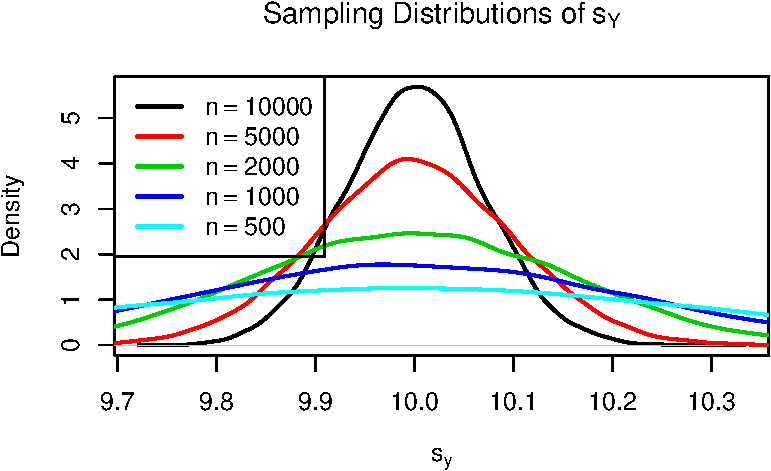
\includegraphics{ITER_files/figure-latex/unnamed-chunk-101-1} \end{center}

The plot shows that the distribution of \(s_Y\) tightens around the true
value \(\sigma_Y = 10\) as \(n\) increases.

The function that estimates the standard deviation of an estimator is
called the \emph{standard error of the estimator}. Key Concept 3.4
summarizes the terminology in the context of the sample mean.

\begin{keyconcepts}[The Standard Error of $\overline{Y}$]{3.4}
Take an i.i.d. sample $Y_1, \dots, Y_n$. The mean of $Y$ is consistently estimated by $\overline{Y}$, the sample mean of the $Y_i$. Since $\overline{Y}$ is a random variable, it has a sampling distribution with variance $\frac{\sigma_Y^2}{n}$.

The standard error of $\overline{Y}$, denoted $SE(\overline{Y})$ is an estimator of the standard deviation of $\overline{Y}$:

$$ SE(\overline{Y}) = \hat\sigma_{\overline{Y}} = \frac{s_Y}{\sqrt{n}} $$

The caret (\string^) over $\sigma$ indicates that $\hat\sigma_{\overline{Y}}$ is an estimator for $\sigma_{\overline{Y}}$. 
\end{keyconcepts}

As an example to underpin Key Concept 3.4, consider a sample of
\(n=100\) i.i.d. observations of the Bernoulli distributed variable
\(Y\) with success probability \(p=0.1\). Thus \(E(Y)=p=0.1\) and
\(\text{Var}(Y)=p(1-p)\). \(E(Y)\) can be estimated by \(\overline{Y}\),
which then has variance

\[ \sigma^2_{\overline{Y}} = p(1-p)/n = 0.0009 \]

and standard deviation

\[ \sigma_{\overline{Y}} = \sqrt{p(1-p)/n} = 0.03. \]

In this case the standard error of \(\overline{Y}\) can be estimated by

\[ SE(\overline{Y}) = \sqrt{\overline{Y}(1-\overline{Y})/n}. \]

Let us check whether \(\overline{Y}\) and \(SE(\overline{Y})\) estimate
the respective true values, on average.

\begin{Shaded}
\begin{Highlighting}[]
\CommentTok{# draw 10000 samples of size 100 and estimate the mean of Y and}
\CommentTok{# estimate the standard error of the sample mean}

\NormalTok{mean_estimates <-}\StringTok{ }\KeywordTok{numeric}\NormalTok{(}\DecValTok{10000}\NormalTok{)}
\NormalTok{se_estimates <-}\StringTok{ }\KeywordTok{numeric}\NormalTok{(}\DecValTok{10000}\NormalTok{)}

\ControlFlowTok{for}\NormalTok{ (i }\ControlFlowTok{in} \DecValTok{1}\OperatorTok{:}\DecValTok{10000}\NormalTok{) \{}
  
\NormalTok{  s <-}\StringTok{ }\KeywordTok{sample}\NormalTok{(}\DecValTok{0}\OperatorTok{:}\DecValTok{1}\NormalTok{, }
              \DataTypeTok{size =} \DecValTok{100}\NormalTok{,  }
              \DataTypeTok{prob =} \KeywordTok{c}\NormalTok{(}\FloatTok{0.9}\NormalTok{, }\FloatTok{0.1}\NormalTok{),}
              \DataTypeTok{replace =}\NormalTok{ T)}
  
\NormalTok{  mean_estimates[i] <-}\StringTok{ }\KeywordTok{mean}\NormalTok{(s)}
\NormalTok{  se_estimates[i] <-}\StringTok{ }\KeywordTok{sqrt}\NormalTok{(}\KeywordTok{mean}\NormalTok{(s) }\OperatorTok{*}\StringTok{ }\NormalTok{(}\DecValTok{1} \OperatorTok{-}\StringTok{ }\KeywordTok{mean}\NormalTok{(s)) }\OperatorTok{/}\StringTok{ }\DecValTok{100}\NormalTok{)}

\NormalTok{\}}

\KeywordTok{mean}\NormalTok{(mean_estimates)}
\end{Highlighting}
\end{Shaded}

\begin{verbatim}
## [1] 0.099693
\end{verbatim}

\begin{Shaded}
\begin{Highlighting}[]
\KeywordTok{mean}\NormalTok{(se_estimates)}
\end{Highlighting}
\end{Shaded}

\begin{verbatim}
## [1] 0.02953467
\end{verbatim}

Both estimators seem to be unbiased for the true parameters. In fact,
this is true for the sample mean, but not for \(SE(\overline{Y})\).
However, both estimators are \emph{consistent} for the true parameters.

\subsection*{Calculating the p-value When the Standard Deviation is
Unknown}\label{calculating-the-p-value-when-the-standard-deviation-is-unknown}
\addcontentsline{toc}{subsection}{Calculating the p-value When the
Standard Deviation is Unknown}

When \(\sigma_Y\) is unknown, the \(p\)-value for a hypothesis test
concerning \(\mu_Y\) using \(\overline{Y}\) can be computed by replacing
\(\sigma_{\overline{Y}}\) in \eqref{eq:pvaluenorm1} by the standard error
\(SE(\overline{Y}) = \hat\sigma_{\overline{Y}}\). Then,

\[ p\text{-value} = 2\cdot\Phi\left(-\left\lvert \frac{\overline{Y}^{act}-\mu_{Y,0}}{SE(\overline{Y})} \right\rvert \right). \]

This is easily done in \texttt{R}:

\begin{Shaded}
\begin{Highlighting}[]
\CommentTok{# sample and estimate, compute standard error}
\NormalTok{samplemean_act <-}\StringTok{ }\KeywordTok{mean}\NormalTok{(}
  \KeywordTok{sample}\NormalTok{(}\DecValTok{0}\OperatorTok{:}\DecValTok{1}\NormalTok{, }
         \DataTypeTok{prob =} \KeywordTok{c}\NormalTok{(}\FloatTok{0.9}\NormalTok{, }\FloatTok{0.1}\NormalTok{), }
         \DataTypeTok{replace =}\NormalTok{ T, }
         \DataTypeTok{size =} \DecValTok{100}\NormalTok{))}

\NormalTok{SE_samplemean <-}\StringTok{ }\KeywordTok{sqrt}\NormalTok{(samplemean_act }\OperatorTok{*}\StringTok{ }\NormalTok{(}\DecValTok{1} \OperatorTok{-}\StringTok{ }\NormalTok{samplemean_act) }\OperatorTok{/}\StringTok{ }\DecValTok{100}\NormalTok{)}

\CommentTok{# null hypothesis}
\NormalTok{mean_h0 <-}\StringTok{ }\FloatTok{0.1}

\CommentTok{# compute the p-value}
\NormalTok{pvalue <-}\StringTok{ }\DecValTok{2} \OperatorTok{*}\StringTok{ }\KeywordTok{pnorm}\NormalTok{(}\OperatorTok{-}\StringTok{ }\KeywordTok{abs}\NormalTok{(samplemean_act }\OperatorTok{-}\StringTok{ }\NormalTok{mean_h0) }\OperatorTok{/}\StringTok{ }\NormalTok{SE_samplemean)}
\NormalTok{pvalue}
\end{Highlighting}
\end{Shaded}

\begin{verbatim}
## [1] 0.5382527
\end{verbatim}

Later in the book, we will encounter more convenient approaches to
obtain \(t\)-statistics and \(p\)-values using \texttt{R}.

\subsection*{The t-statistic}\label{the-t-statistic}
\addcontentsline{toc}{subsection}{The t-statistic}

In hypothesis testing, the standardized sample average

\begin{equation}
t = \frac{\overline{Y} - \mu_{Y,0}}{SE(\overline{Y})} \label{eq:tstat}
\end{equation}

is called a \(t\)-statistic. This \(t\)-statistic plays an important
role in testing hypotheses about \(\mu_Y\). It is a prominent example of
a test statistic.

Implicitly, we already have computed a \(t\)-statistic for
\(\overline{Y}\) in the previous code chunk.

\begin{Shaded}
\begin{Highlighting}[]
\CommentTok{# compute a t-statistic for the sample mean}
\NormalTok{tstatistic <-}\StringTok{ }\NormalTok{(samplemean_act }\OperatorTok{-}\StringTok{ }\NormalTok{mean_h0) }\OperatorTok{/}\StringTok{ }\NormalTok{SE_samplemean}
\NormalTok{tstatistic}
\end{Highlighting}
\end{Shaded}

\begin{verbatim}
## [1] 0.6154575
\end{verbatim}

Using \texttt{R} we can illustrate that if \(\mu_{Y,0}\) equals the true
value, that is, if the null hypothesis is true, \eqref{eq:tstat} is
approximately \(\mathcal{N}(0,1)\) distributed when \(n\) is large.

\begin{Shaded}
\begin{Highlighting}[]
\CommentTok{# prepare empty vector for t-statistics}
\NormalTok{tstatistics <-}\StringTok{ }\KeywordTok{numeric}\NormalTok{(}\DecValTok{10000}\NormalTok{)}

\CommentTok{# set sample size}
\NormalTok{n <-}\StringTok{ }\DecValTok{300}

\CommentTok{# simulate 10000 t-statistics}
\ControlFlowTok{for}\NormalTok{ (i }\ControlFlowTok{in} \DecValTok{1}\OperatorTok{:}\DecValTok{10000}\NormalTok{) \{}
  
\NormalTok{  s <-}\StringTok{ }\KeywordTok{sample}\NormalTok{(}\DecValTok{0}\OperatorTok{:}\DecValTok{1}\NormalTok{, }
              \DataTypeTok{size =}\NormalTok{ n,  }
              \DataTypeTok{prob =} \KeywordTok{c}\NormalTok{(}\FloatTok{0.9}\NormalTok{, }\FloatTok{0.1}\NormalTok{),}
              \DataTypeTok{replace =}\NormalTok{ T)}
  
\NormalTok{  tstatistics[i] <-}\StringTok{ }\NormalTok{(}\KeywordTok{mean}\NormalTok{(s)}\OperatorTok{-}\FloatTok{0.1}\NormalTok{)}\OperatorTok{/}\KeywordTok{sqrt}\NormalTok{(}\KeywordTok{var}\NormalTok{(s)}\OperatorTok{/}\NormalTok{n)}
  
\NormalTok{\}}
\end{Highlighting}
\end{Shaded}

In the simulation above we estimate the variance of the \(Y_i\) using
\texttt{var(s)}. This is more general then \texttt{mean(s)*(1-mean(s))}
since the latter requires that the data are Bernoulli distributed and
that we know this.

\begin{Shaded}
\begin{Highlighting}[]
\CommentTok{# plot density and compare to N(0,1) density}
\KeywordTok{plot}\NormalTok{(}\KeywordTok{density}\NormalTok{(tstatistics),}
     \DataTypeTok{xlab =} \StringTok{'t-statistic'}\NormalTok{,}
     \DataTypeTok{main =} \StringTok{'Estimated Distribution of the t-statistic when n=300'}\NormalTok{,}
     \DataTypeTok{lwd =} \DecValTok{2}\NormalTok{,}
     \DataTypeTok{xlim =} \KeywordTok{c}\NormalTok{(}\OperatorTok{-}\DecValTok{4}\NormalTok{, }\DecValTok{4}\NormalTok{),}
     \DataTypeTok{col =} \StringTok{'steelblue'}\NormalTok{)}

\CommentTok{# N(0,1) density (dashed)}
\KeywordTok{curve}\NormalTok{(}\KeywordTok{dnorm}\NormalTok{(x), }
      \DataTypeTok{add =}\NormalTok{ T, }
      \DataTypeTok{lty =} \DecValTok{2}\NormalTok{, }
      \DataTypeTok{lwd =} \DecValTok{2}\NormalTok{)}
\end{Highlighting}
\end{Shaded}

\begin{center}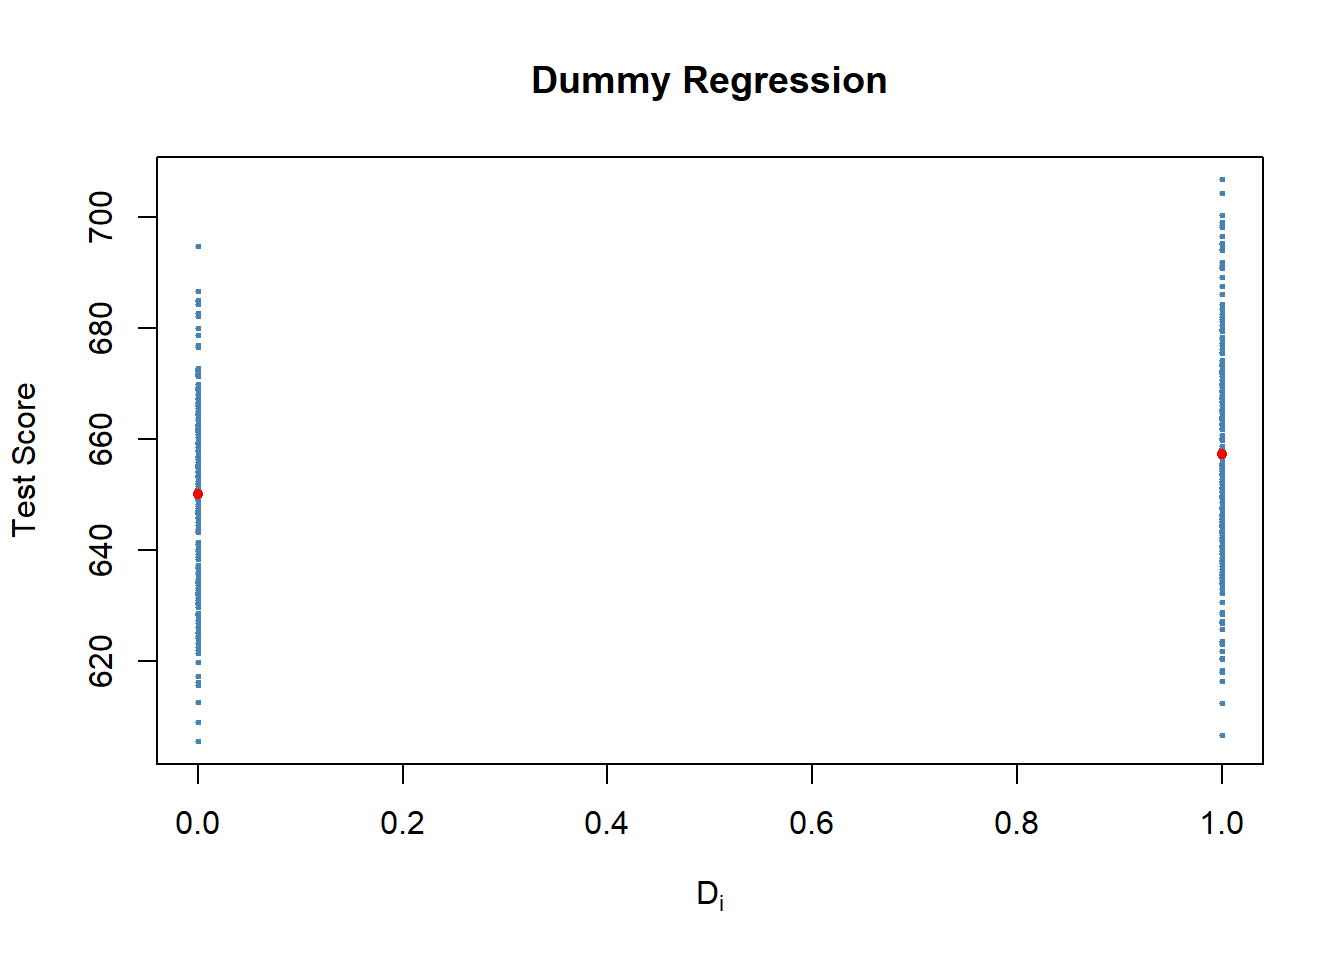
\includegraphics{ITER_files/figure-latex/unnamed-chunk-108-1} \end{center}

Judging from the plot, the normal approximation works reasonably well
for the chosen sample size. This normal approximation has already been
used in the definition of the \(p\)-value, see \eqref{eq:tstat}.

\subsection*{Hypothesis Testing with a Prespecified Significance
Level}\label{hypothesis-testing-with-a-prespecified-significance-level}
\addcontentsline{toc}{subsection}{Hypothesis Testing with a Prespecified
Significance Level}

\begin{keyconcepts}[The Terminology of Hypothesis Testing]{3.5}
In hypothesis testing, two types of mistakes are possible:\newline

\begin{enumerate}
\item The null hypothesis \textit{is} rejected although it is true (type-I-error)  
\item The null hypothesis \textit{is not} rejected although it is false (type-II-error) 
\end{enumerate}\vspace{0.5cm}

The \textit{significance level} of the test is the probability to commit a type-I-error we are willing to accept in advance. E.g., using a prespecified significance level of $0.05$, we reject the null hypothesis if and only if the $p$-value is less than $0.05$. The significance level is chosen before the test is conducted.\newline

An equivalent procedure is to reject the null hypothesis if the observed test statistic is, in absolute value terms, larger than the \textit{critical value} of the test statistic. The critical value is determined by the significance level chosen and defines two disjoint sets of values which are called \textit{acceptance region} and \textit{rejection region}. The acceptance region contains all values of the test statistic for which the test does not reject while the rejection region contains all the values for which the test does reject.\newline

The \textit{$p$-value} is the probability that, in repeated sampling under the same conditions, a test statistic is observed that provides just as much evidence against the null hypothesis as the test statistic actually observed.\newline

The actual probability that the test rejects the true null hypothesis is called the \textit{size of the test}. In an ideal setting, the size equals the significance level.\newline

The probability that the test correctly rejects a false null hypothesis is called \textit{power}. 
\end{keyconcepts}

Reconsider the \texttt{pvalue} computed further above:

\begin{Shaded}
\begin{Highlighting}[]
\CommentTok{# check whether p-value < 0.05}
\NormalTok{pvalue }\OperatorTok{<}\StringTok{ }\FloatTok{0.05}
\end{Highlighting}
\end{Shaded}

\begin{verbatim}
## [1] FALSE
\end{verbatim}

The condition is not fulfilled so we do not reject the null hypothesis
correctly.

When working with a \(t\)-statistic instead, it is equivalent to apply
the following rule:

\[ \text{Reject } H_0 \text{ if } \lvert t^{act} \rvert > 1.96 \]

We reject the null hypothesis at the significance level of \(5\%\) if
the computed \(t\)-statistic lies beyond the critical value of 1.96 in
absolute value terms. \(1.96\) is the \(0.975\)-quantile of the standard
normal distribution.

\begin{Shaded}
\begin{Highlighting}[]
\CommentTok{# check the critical value}
\KeywordTok{qnorm}\NormalTok{(}\DataTypeTok{p =} \FloatTok{0.975}\NormalTok{)}
\end{Highlighting}
\end{Shaded}

\begin{verbatim}
## [1] 1.959964
\end{verbatim}

\begin{Shaded}
\begin{Highlighting}[]
\CommentTok{# check whether the null is rejected using the t-statistic computed further above}
\KeywordTok{abs}\NormalTok{(tstatistic) }\OperatorTok{>}\StringTok{ }\FloatTok{1.96}
\end{Highlighting}
\end{Shaded}

\begin{verbatim}
## [1] FALSE
\end{verbatim}

Just like using the \(p\)-value, we cannot reject the null hypothesis
using the corresponding \(t\)-statistic. Key Concept 3.6 summarizes the
procedure of performing a two-sided hypothesis test about the population
mean \(E(Y)\).

\begin{keyconcepts}[Testing the Hypothesis $E(Y) = \mu_{Y,0}$ Against the Alternative $E(Y) \neq \mu_{Y,0}$]{3.6}
\begin{enumerate}
\item Estimate $\mu_{Y}$ using $\overline{Y}$ and compute $SE(\overline{Y})$, the standard error of $SE(\overline{Y})$.
\item Compute the $t$-statistic.
\item Compute the $p$-value and reject the null hypothesis at the $5\%$ level of significance if the $p$-value is smaller than $0.05$ or, equivalently, if $$\left\lvert t^{act} \right\rvert > 1.96.$$
\end{enumerate}
\end{keyconcepts}

\subsection*{One-sided Alternatives}\label{one-sided-alternatives}
\addcontentsline{toc}{subsection}{One-sided Alternatives}

Sometimes we are interested in testing if the mean is bigger or smaller
than some value hypothesized under the null. To stick to the book, take
the presumed wage gap between well and less educated working
individuals. Since we anticipate that such a differential exists, a
relevant alternative (to the null hypothesis that there is no wage
differential) is that well educated individuals earn more, i.e., that
the average hourly wage for this group, \(\mu_Y\) is \emph{bigger} than
\(\mu_{Y,0}\), the average wage of less educated workers which we assume
to be known here for simplicity (Section @ref\{cmfdp\} discusses how to
test the equivalence of to unknown population means).

This is an example of a \emph{right-sided test} and the hypotheses pair
is chosen to be

\[ H_0: \mu_Y = \mu_{Y,0} \ \ \text{vs} \ \ H_1: \mu_Y > \mu_{Y,0}. \]

We reject the null hypothesis if the computed test-statistic is larger
than the critical value \(1.64\), the \(0.95\)-quantile of the
\(\mathcal{N}(0,1)\) distribution. This ensures that \(1-0.95=5\%\)
probability mass remains in the area to the right of the critical value.
As before, we can visualize this in \texttt{R} using the function
\texttt{polygon()}.

\begin{Shaded}
\begin{Highlighting}[]
\CommentTok{# plot the standard normal density on the domain [-4,4]}
\KeywordTok{curve}\NormalTok{(}\KeywordTok{dnorm}\NormalTok{(x),}
      \DataTypeTok{xlim =} \KeywordTok{c}\NormalTok{(}\OperatorTok{-}\DecValTok{4}\NormalTok{, }\DecValTok{4}\NormalTok{),}
      \DataTypeTok{main =} \StringTok{'Rejection Region of a Right-Sided Test'}\NormalTok{,}
      \DataTypeTok{yaxs =} \StringTok{'i'}\NormalTok{,}
      \DataTypeTok{xlab =} \StringTok{'t-statistic'}\NormalTok{,}
      \DataTypeTok{ylab =} \StringTok{''}\NormalTok{,}
      \DataTypeTok{lwd =} \DecValTok{2}\NormalTok{,}
      \DataTypeTok{axes =} \StringTok{'F'}\NormalTok{)}

\CommentTok{# add the x-axis}
\KeywordTok{axis}\NormalTok{(}\DecValTok{1}\NormalTok{, }
     \DataTypeTok{at =} \KeywordTok{c}\NormalTok{(}\OperatorTok{-}\DecValTok{4}\NormalTok{, }\DecValTok{0}\NormalTok{, }\FloatTok{1.64}\NormalTok{, }\DecValTok{4}\NormalTok{), }
     \DataTypeTok{padj =} \FloatTok{0.5}\NormalTok{,}
     \DataTypeTok{labels =} \KeywordTok{c}\NormalTok{(}\StringTok{''}\NormalTok{, }\DecValTok{0}\NormalTok{, }\KeywordTok{expression}\NormalTok{(Phi}\OperatorTok{^-}\DecValTok{1}\OperatorTok{~}\NormalTok{(.}\DecValTok{95}\NormalTok{)}\OperatorTok{==}\FloatTok{1.64}\NormalTok{), }\StringTok{''}\NormalTok{))}

\CommentTok{# shade the rejection region in the left tail}
\KeywordTok{polygon}\NormalTok{(}\DataTypeTok{x =} \KeywordTok{c}\NormalTok{(}\FloatTok{1.64}\NormalTok{, }\KeywordTok{seq}\NormalTok{(}\FloatTok{1.64}\NormalTok{, }\DecValTok{4}\NormalTok{, }\FloatTok{0.01}\NormalTok{), }\DecValTok{4}\NormalTok{),}
        \DataTypeTok{y =} \KeywordTok{c}\NormalTok{(}\DecValTok{0}\NormalTok{, }\KeywordTok{dnorm}\NormalTok{(}\KeywordTok{seq}\NormalTok{(}\FloatTok{1.64}\NormalTok{, }\DecValTok{4}\NormalTok{, }\FloatTok{0.01}\NormalTok{)), }\DecValTok{0}\NormalTok{), }
        \DataTypeTok{col =} \StringTok{'darkred'}\NormalTok{)}
\end{Highlighting}
\end{Shaded}

\begin{center}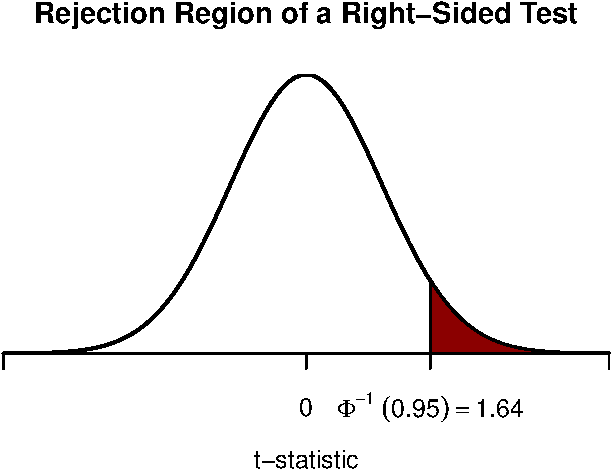
\includegraphics{ITER_files/figure-latex/unnamed-chunk-115-1} \end{center}

Analogously, for the left-sided test we have
\[H_0: \mu_Y = \mu_{Y,0} \ \ \text{vs.} \ \ H_1: \mu_Y < \mu_{Y,0}.\]
The null is rejected if the observed test statistic falls short of the
critical value which, for a test at the \(0.05\) level of significance,
is given by \(-1.64\), the \(0.05\)-quantile of the \(\mathcal{N}(0,1)\)
distribution. \(5\%\) probability mass lies to the left of the critical
value.

It is straightforward to adapt the code chunk above to the case of a
left-sided test. We only have to adjust the color shading and the tick
marks.

\begin{Shaded}
\begin{Highlighting}[]
\CommentTok{# plot the the standard normal density on the domain [-4,4]}
\KeywordTok{curve}\NormalTok{(}\KeywordTok{dnorm}\NormalTok{(x),}
      \DataTypeTok{xlim =} \KeywordTok{c}\NormalTok{(}\OperatorTok{-}\DecValTok{4}\NormalTok{, }\DecValTok{4}\NormalTok{),}
      \DataTypeTok{main =} \StringTok{'Rejection Region of a Left-Sided Test'}\NormalTok{,}
      \DataTypeTok{yaxs =} \StringTok{'i'}\NormalTok{,}
      \DataTypeTok{xlab =} \StringTok{'t-statistic'}\NormalTok{,}
      \DataTypeTok{ylab =} \StringTok{''}\NormalTok{,}
      \DataTypeTok{lwd =} \DecValTok{2}\NormalTok{,}
      \DataTypeTok{axes =} \StringTok{'F'}\NormalTok{)}

\CommentTok{# add x-axis}
\KeywordTok{axis}\NormalTok{(}\DecValTok{1}\NormalTok{, }
     \DataTypeTok{at =} \KeywordTok{c}\NormalTok{(}\OperatorTok{-}\DecValTok{4}\NormalTok{, }\DecValTok{0}\NormalTok{, }\OperatorTok{-}\FloatTok{1.64}\NormalTok{, }\DecValTok{4}\NormalTok{), }
     \DataTypeTok{padj =} \FloatTok{0.5}\NormalTok{,}
     \DataTypeTok{labels =} \KeywordTok{c}\NormalTok{(}\StringTok{''}\NormalTok{, }\DecValTok{0}\NormalTok{, }\KeywordTok{expression}\NormalTok{(Phi}\OperatorTok{^-}\DecValTok{1}\OperatorTok{~}\NormalTok{(.}\DecValTok{05}\NormalTok{)}\OperatorTok{==-}\FloatTok{1.64}\NormalTok{), }\StringTok{''}\NormalTok{))}

\CommentTok{# shade rejection region in right tail}
\KeywordTok{polygon}\NormalTok{(}\DataTypeTok{x =} \KeywordTok{c}\NormalTok{(}\OperatorTok{-}\DecValTok{4}\NormalTok{, }\KeywordTok{seq}\NormalTok{(}\OperatorTok{-}\DecValTok{4}\NormalTok{, }\OperatorTok{-}\FloatTok{1.64}\NormalTok{, }\FloatTok{0.01}\NormalTok{), }\OperatorTok{-}\FloatTok{1.64}\NormalTok{),}
        \DataTypeTok{y =} \KeywordTok{c}\NormalTok{(}\DecValTok{0}\NormalTok{, }\KeywordTok{dnorm}\NormalTok{(}\KeywordTok{seq}\NormalTok{(}\OperatorTok{-}\DecValTok{4}\NormalTok{, }\OperatorTok{-}\FloatTok{1.64}\NormalTok{, }\FloatTok{0.01}\NormalTok{)), }\DecValTok{0}\NormalTok{), }
        \DataTypeTok{col =} \StringTok{'darkred'}\NormalTok{)}
\end{Highlighting}
\end{Shaded}

\begin{center}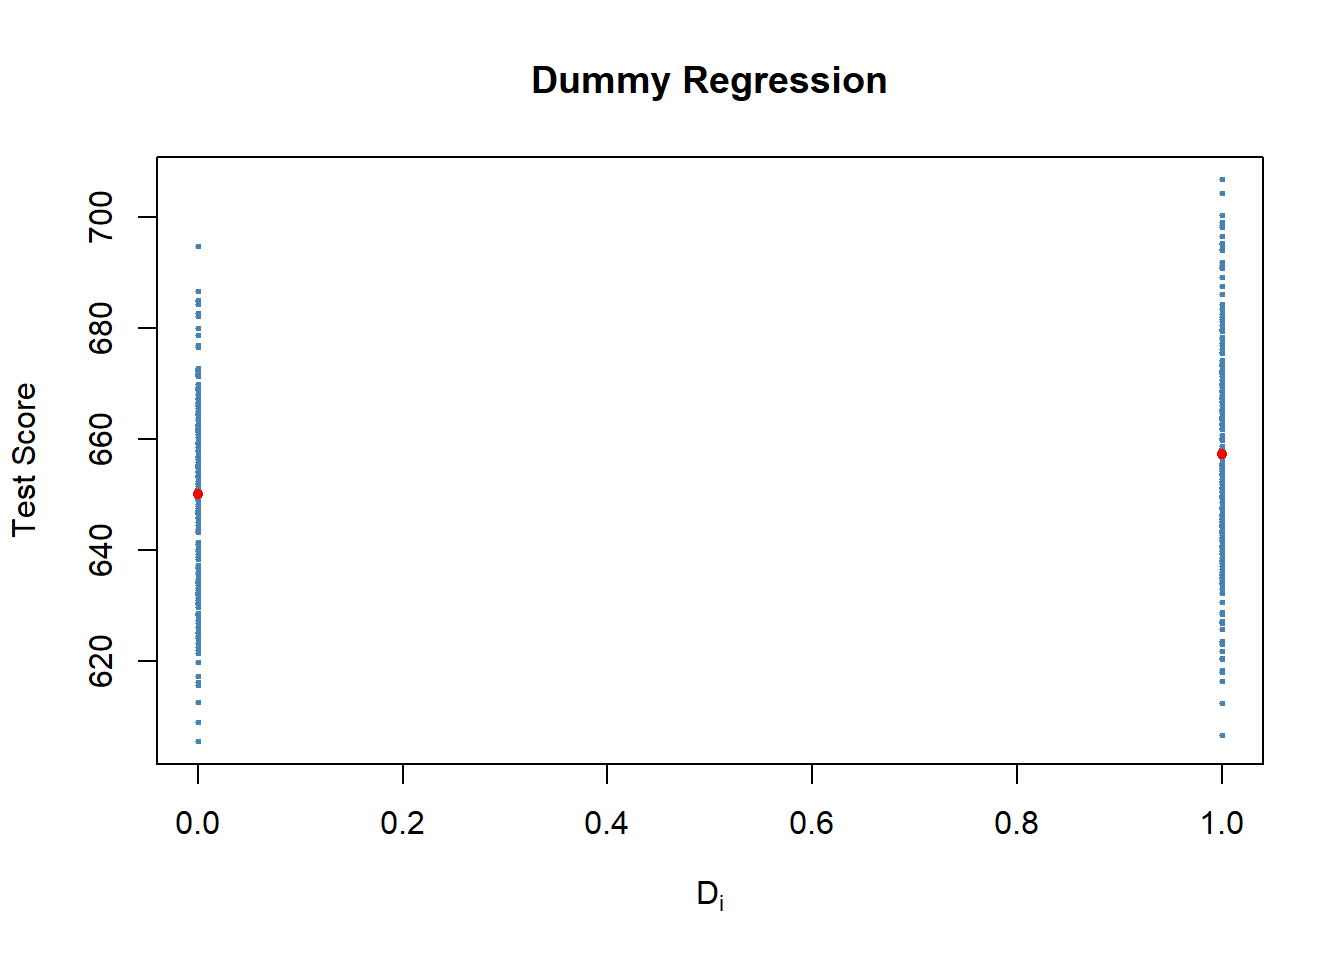
\includegraphics{ITER_files/figure-latex/unnamed-chunk-116-1} \end{center}

\section{Confidence Intervals for the Population
Mean}\label{confidence-intervals-for-the-population-mean}

As stressed before, we will never estimate the \emph{exact} value of the
population mean of \(Y\) using a random sample. However, we can compute
confidence intervals for the population mean. In general, a confidence
interval for an unknown parameter is a recipe that, in repeated samples,
yields intervals that contain the true parameter with a prespecified
probability, the \emph{confidence level}. Confidence intervals are
computed using the information available in the sample. Since this
information is the result of a random process, confidence intervals are
random variables themselves.

Key Concept 3.7 shows how to compute confidence intervals for the
unknown population mean \(E(Y)\).

\begin{keyconcepts}[Confidence Intervals for the Population Mean]{3.7}
A $95\%$ confidence interval for $\mu_Y$ is a \texttt{random variable} that contains the true $\mu_Y$ in $95\%$ of all possible random samples. When $n$ is large we can use the normal approximation. Then, $99\%$, $95\%$, $90\%$ confidence intervals are

\begin{align}
&99\%\text{ confidence interval for } \mu_Y = \left[ \overline{Y} \pm 2.58 \times SE(\overline{Y}) \right], \\
&95\%\text{ confidence interval for } \mu_Y = \left[\overline{Y} \pm 1.96 \times SE(\overline{Y}) \right], \\
&90\%\text{ confidence interval for } \mu_Y = \left[ \overline{Y} \pm 1.64 \times SE(\overline{Y}) \right].
\end{align}

These confidence intervals are sets of null hypotheses we cannot reject in a two-sided hypothesis test at the given level of confidence.\newline

Now consider the following statements.\newline

\begin{enumerate}
\item In repeated sampling, the interval
$$ \left[ \overline{Y} \pm 1.96 \times SE(\overline{Y}) \right] $$
covers the true value of $\mu_Y$ with a probability of $95\%$.

\item We have computed $\overline{Y} = 5.1$ and $SE(\overline{Y})=2.5$ so the interval
$$ \left[5.1  \pm 1.96 \times 2.5 \right] = \left[0.2,10\right] $$ covers the true value of $\mu_Y$ with a probability of $95\%$.
\end{enumerate}\vspace{0.5cm}

While 1. is right (this is in line with the definition above), 2. is wrong and none of your lecturers wants to read such a sentence in a term paper, written exam or similar, believe us.
The difference is that, while 1. is the definition of a random variable, 2. is one possible \textit{outcome} of this random variable so there is no meaning in making any probabilistic statement about it. Either the computed interval \textit{does cover} $\mu_Y$ or it \textit{does not}!
\end{keyconcepts}

In \texttt{R}, testing of hypotheses about the mean of a population on
the basis of a random sample is very easy due to functions like
\texttt{t.test()} from the \texttt{stats} package. It produces an object
of type \texttt{list}. Luckily, one of the most simple ways to use
\texttt{t.test()} is when you want to obtain a \(95\%\) confidence
interval for some population mean. We start by generating some random
data and calling \texttt{t.test()} in conjunction with \texttt{ls()} to
obtain a breakdown of the output components.

\begin{Shaded}
\begin{Highlighting}[]
\CommentTok{# set seed}
\KeywordTok{set.seed}\NormalTok{(}\DecValTok{1}\NormalTok{)}

\CommentTok{# generate some sample data}
\NormalTok{sampledata <-}\StringTok{ }\KeywordTok{rnorm}\NormalTok{(}\DecValTok{100}\NormalTok{, }\DecValTok{10}\NormalTok{, }\DecValTok{10}\NormalTok{)}

\CommentTok{# check the type of the outcome produced by t.test}
\KeywordTok{typeof}\NormalTok{(}\KeywordTok{t.test}\NormalTok{(sampledata))}
\end{Highlighting}
\end{Shaded}

\begin{verbatim}
## [1] "list"
\end{verbatim}

\begin{Shaded}
\begin{Highlighting}[]
\CommentTok{# display the list elements produced by t.test}
\KeywordTok{ls}\NormalTok{(}\KeywordTok{t.test}\NormalTok{(sampledata))}
\end{Highlighting}
\end{Shaded}

\begin{verbatim}
## [1] "alternative" "conf.int"    "data.name"   "estimate"    "method"     
## [6] "null.value"  "p.value"     "parameter"   "statistic"
\end{verbatim}

Though we find that many items are reported, at the moment we are only
interested in computing a \(95\%\) confidence set for the mean.

\begin{Shaded}
\begin{Highlighting}[]
\KeywordTok{t.test}\NormalTok{(sampledata)}\OperatorTok{$}\StringTok{"conf.int"}
\end{Highlighting}
\end{Shaded}

\begin{verbatim}
## [1]  9.306651 12.871096
## attr(,"conf.level")
## [1] 0.95
\end{verbatim}

This tells us that the \(95\%\) confidence interval is

\[ \left[9.31, 12.87\right]. \]

In this example, the computed interval obviously does cover the true
\(\mu_Y\) which we know to be \(10\).

Let us have a look at the whole standard output produced by
\texttt{t.test()}.

\begin{Shaded}
\begin{Highlighting}[]
\KeywordTok{t.test}\NormalTok{(sampledata)}
\end{Highlighting}
\end{Shaded}

\begin{verbatim}
## 
##  One Sample t-test
## 
## data:  sampledata
## t = 12.346, df = 99, p-value < 2.2e-16
## alternative hypothesis: true mean is not equal to 0
## 95 percent confidence interval:
##   9.306651 12.871096
## sample estimates:
## mean of x 
##  11.08887
\end{verbatim}

We see that \texttt{t.test()} does not only compute a \(95\%\)
confidence interval but automatically conducts a two-sided significance
test of the hypothesis \(H_0: \mu_Y = 0\) at the level of \(5\%\) and
reports relevant parameters thereof: the alternative hypothesis, the
estimated mean, the resulting \(t\)-statistic, the degrees of freedom of
the underlying \(t\) distribution (\texttt{t.test()} does use perform
the normal approximation) and the corresponding \(p\)-value. This is
very convenient!

In this example, we come to the conclusion that the population mean
\emph{is} significantly different from \(0\) (which is correct) at the
level of \(5\%\), since \(\mu_Y = 0\) is not an element of the \(95\%\)
confidence interval

\[ 0 \in \left[9.31,12.87\right]. \] We come to an equivalent result
when using the \(p\)-value rejection rule since

\[ p\text{-value} = 2.2\cdot 10^{-16} \ll 0.05. \]

\section{Comparing Means from Different Populations}\label{cmfdp}

Suppose you are interested in the means of two different populations,
denote them \(\mu_1\) and \(\mu_2\). More specifically, you are
interested whether these population means are different from each other
and plan to use a hypothesis test to verify this on the basis of
independent sample data from both populations. A suitable pair of
hypotheses is

\begin{equation}
H_0: \mu_1 - \mu_2 = d_0 \ \ \text{vs.} \ \ H_1: \mu_1 - \mu_2 \neq d_0 \label{eq:hypmeans}
\end{equation}

where \(d_0\) denotes the hypothesized difference in means (so \(d_0=0\)
when the means are equal, under the null hypothesis). The book teaches
us that \(H_0\) can be tested with the \(t\)-statistic

\begin{equation}
t=\frac{(\overline{Y}_1 - \overline{Y}_2) - d_0}{SE(\overline{Y}_1 - \overline{Y}_2)} \label{eq:tstatmeans}
\end{equation}

where

\begin{equation}
SE(\overline{Y}_1 - \overline{Y}_2) = \sqrt{\frac{s_1^2}{n_1} + \frac{s_2^2}{n_2}}.
\end{equation}

This is called a two sample \(t\)-test. For large \(n_1\) and \(n_2\),
\eqref{eq:tstatmeans} is standard normal under the null hypothesis.
Analogously to the simple \(t\)-test we can compute confidence intervals
for the true difference in population means:

\[ (\overline{Y}_1 - \overline{Y}_2) \pm 1.96 \times SE(\overline{Y}_1 - \overline{Y}_2) \]

is a \(95\%\) confidence interval for \(d\). In \texttt{R}, hypotheses
as in \eqref{eq:hypmeans} can be tested with \texttt{t.test()}, too. Note
that \texttt{t.test()} chooses \(d_0 = 0\) by default. This can be
changed by setting the argument \texttt{mu} accordingly.

The subsequent code chunk demonstrates how to perform a two sample
\(t\)-test in \texttt{R} using simulated data.

\begin{Shaded}
\begin{Highlighting}[]
\CommentTok{# set random seed}
\KeywordTok{set.seed}\NormalTok{(}\DecValTok{1}\NormalTok{)}

\CommentTok{# draw data from two different populations with equal mean}
\NormalTok{sample_pop1 <-}\StringTok{ }\KeywordTok{rnorm}\NormalTok{(}\DecValTok{100}\NormalTok{, }\DecValTok{10}\NormalTok{, }\DecValTok{10}\NormalTok{)}
\NormalTok{sample_pop2 <-}\StringTok{ }\KeywordTok{rnorm}\NormalTok{(}\DecValTok{100}\NormalTok{, }\DecValTok{10}\NormalTok{, }\DecValTok{20}\NormalTok{)}

\CommentTok{# perform a two sample t-test}
\KeywordTok{t.test}\NormalTok{(sample_pop1, sample_pop2)}
\end{Highlighting}
\end{Shaded}

\begin{verbatim}
## 
##  Welch Two Sample t-test
## 
## data:  sample_pop1 and sample_pop2
## t = 0.872, df = 140.52, p-value = 0.3847
## alternative hypothesis: true difference in means is not equal to 0
## 95 percent confidence interval:
##  -2.338012  6.028083
## sample estimates:
## mean of x mean of y 
## 11.088874  9.243838
\end{verbatim}

We find that the two sample \(t\)-test does not reject the (true) null
hypothesis that \(d_0 = 0\).

\section{An Application to the Gender Gap of Earnings}\label{aattggoe}

This section discusses how to reproduce the results presented in the box
\emph{The Gender Gap of Earnings of College Graduates in the United
States} of the book.

In order to reproduce Table 3.1 of the book you need to download the
replication data which are hosted by Pearson and can be downloaded
\href{http://wps.aw.com/aw_stock_ie_3/178/45691/11696965.cw/index.html}{here}.
Download the data for Chapter 3 as an excel spreadsheet
(\texttt{cps\_ch3.xlsx}). This dataset contains data that range from
\(1992\) to \(2008\) and earnings are reported in prices of \(2008\).
There are several ways to import the \texttt{.xlsx}-files into
\texttt{R}. Our suggestion is the function \texttt{read\_excel()} from
the \texttt{readxl} package \citep{R-readxl}. The package is not part of
\texttt{R}'s base version and has to be installed manually.

\begin{Shaded}
\begin{Highlighting}[]
\CommentTok{# load the 'readxl' package}
\KeywordTok{library}\NormalTok{(readxl)}
\end{Highlighting}
\end{Shaded}

You are now ready to import the dataset. Make sure you use the correct
path to import the downloaded file! In our example, the file is saved in
a sub folder (\texttt{data}) of the working directory. If you are not
sure what your current working directory is, use \texttt{getwd()}, see
also \texttt{?getwd}. This will give you the path that points to the
place \texttt{R} is currently looking for files.

\begin{Shaded}
\begin{Highlighting}[]
\CommentTok{# import the data into R}
\NormalTok{cps <-}\StringTok{ }\KeywordTok{read_excel}\NormalTok{(}\DataTypeTok{path =} \StringTok{'data/cps_ch3.xlsx'}\NormalTok{)}
\end{Highlighting}
\end{Shaded}

Next, install and load the package \texttt{dyplr} \citep{R-dplyr}. This
package provides some handy functions that simplify data wrangling a
lot. It makes use of the \texttt{\%>\%} operator.

\begin{Shaded}
\begin{Highlighting}[]
\CommentTok{# load the 'dplyr' package}
\KeywordTok{library}\NormalTok{(dplyr)}
\end{Highlighting}
\end{Shaded}

First, get an overview over the dataset. Next, use \texttt{\%>\%} and
some functions from the \texttt{dplyr} package to group the observations
by gender and year and compute descriptive statistics for both groups.

\begin{Shaded}
\begin{Highlighting}[]
\CommentTok{# get an overview of the data structure}
\KeywordTok{head}\NormalTok{(cps)}
\end{Highlighting}
\end{Shaded}

\begin{verbatim}
## # A tibble: 6 x 3
##   a_sex  year ahe08
##   <dbl> <dbl> <dbl>
## 1     1  1992  17.2
## 2     1  1992  15.3
## 3     1  1992  22.9
## 4     2  1992  13.3
## 5     1  1992  22.1
## 6     2  1992  12.2
\end{verbatim}

\begin{Shaded}
\begin{Highlighting}[]
\CommentTok{# group data by gender and year and compute the mean, standard deviation}
\CommentTok{# and number of observations for each group}
\NormalTok{avgs <-}\StringTok{ }\NormalTok{cps }\OperatorTok\StringTok{ }
\StringTok{        }\KeywordTok{group_by}\NormalTok{(a_sex, year) }\OperatorTok\StringTok{ }
\StringTok{        }\KeywordTok{summarise}\NormalTok{(}\KeywordTok{mean}\NormalTok{(ahe08), }
                  \KeywordTok{sd}\NormalTok{(ahe08), }
                  \KeywordTok{n}\NormalTok{())}

\CommentTok{# print the results to the console}
\KeywordTok{print}\NormalTok{(avgs)}
\end{Highlighting}
\end{Shaded}

\begin{verbatim}
## # A tibble: 10 x 5
## # Groups:   a_sex [?]
##    a_sex  year `mean(ahe08)` `sd(ahe08)` `n()`
##    <dbl> <dbl>         <dbl>       <dbl> <int>
##  1     1  1992          23.3       10.2   1594
##  2     1  1996          22.5       10.1   1379
##  3     1  2000          24.9       11.6   1303
##  4     1  2004          25.1       12.0   1894
##  5     1  2008          25.0       11.8   1838
##  6     2  1992          20.0        7.87  1368
##  7     2  1996          19.0        7.95  1230
##  8     2  2000          20.7        9.36  1181
##  9     2  2004          21.0        9.36  1735
## 10     2  2008          20.9        9.66  1871
\end{verbatim}

With the pipe operator \texttt{\%>\%} we simply chain different
\texttt{R} functions that produce compatible input and output. In the
code above, we take the dataset \texttt{cps} and use it as an input for
the function \texttt{group\_by()}. The output of \texttt{group\_by} is
subsequently used as an input for \texttt{summarise()} and so forth.

Now that we have computed the statistics of interest for both genders,
we can investigate how the gap in earnings between both groups evolves
over time.

\begin{Shaded}
\begin{Highlighting}[]
\CommentTok{# split the dataset by gender}
\NormalTok{male <-}\StringTok{ }\NormalTok{avgs }\OperatorTok\StringTok{ }\KeywordTok{filter}\NormalTok{(a_sex }\OperatorTok{==}\StringTok{ }\DecValTok{1}\NormalTok{) }
\NormalTok{female <-}\StringTok{ }\NormalTok{avgs }\OperatorTok\StringTok{ }\KeywordTok{filter}\NormalTok{(a_sex }\OperatorTok{==}\StringTok{ }\DecValTok{2}\NormalTok{)}

\CommentTok{# rename columns of both splits}
\KeywordTok{colnames}\NormalTok{(male)   <-}\StringTok{ }\KeywordTok{c}\NormalTok{(}\StringTok{"Sex"}\NormalTok{, }\StringTok{"Year"}\NormalTok{, }\StringTok{"Y_bar_m"}\NormalTok{, }\StringTok{"s_m"}\NormalTok{, }\StringTok{"n_m"}\NormalTok{)}
\KeywordTok{colnames}\NormalTok{(female) <-}\StringTok{ }\KeywordTok{c}\NormalTok{(}\StringTok{"Sex"}\NormalTok{, }\StringTok{"Year"}\NormalTok{, }\StringTok{"Y_bar_f"}\NormalTok{, }\StringTok{"s_f"}\NormalTok{, }\StringTok{"n_f"}\NormalTok{)}

\CommentTok{# estimate gender gaps, compute standard errors and confidence intervals for all dates}
\NormalTok{gap <-}\StringTok{ }\NormalTok{male}\OperatorTok{$}\NormalTok{Y_bar_m }\OperatorTok{-}\StringTok{ }\NormalTok{female}\OperatorTok{$}\NormalTok{Y_bar_f}

\NormalTok{gap_se <-}\StringTok{ }\KeywordTok{sqrt}\NormalTok{(male}\OperatorTok{$}\NormalTok{s_m}\OperatorTok{^}\DecValTok{2} \OperatorTok{/}\StringTok{ }\NormalTok{male}\OperatorTok{$}\NormalTok{n_m }\OperatorTok{+}\StringTok{ }\NormalTok{female}\OperatorTok{$}\NormalTok{s_f}\OperatorTok{^}\DecValTok{2} \OperatorTok{/}\StringTok{ }\NormalTok{female}\OperatorTok{$}\NormalTok{n_f)}

\NormalTok{gap_ci_l <-}\StringTok{ }\NormalTok{gap }\OperatorTok{-}\StringTok{ }\FloatTok{1.96} \OperatorTok{*}\StringTok{ }\NormalTok{gap_se}

\NormalTok{gap_ci_u <-}\StringTok{ }\NormalTok{gap }\OperatorTok{+}\StringTok{ }\FloatTok{1.96} \OperatorTok{*}\StringTok{ }\NormalTok{gap_se}

\NormalTok{result <-}\StringTok{ }\KeywordTok{cbind}\NormalTok{(male[,}\OperatorTok{-}\DecValTok{1}\NormalTok{], female[,}\OperatorTok{-}\NormalTok{(}\DecValTok{1}\OperatorTok{:}\DecValTok{2}\NormalTok{)], gap, gap_se, gap_ci_l, gap_ci_u)}

\CommentTok{# print the results to the console}
\KeywordTok{print}\NormalTok{(result, }\DataTypeTok{digits =} \DecValTok{3}\NormalTok{)}
\end{Highlighting}
\end{Shaded}

\begin{verbatim}
##   Year Y_bar_m  s_m  n_m Y_bar_f  s_f  n_f  gap gap_se gap_ci_l gap_ci_u
## 1 1992    23.3 10.2 1594    20.0 7.87 1368 3.23  0.332     2.58     3.88
## 2 1996    22.5 10.1 1379    19.0 7.95 1230 3.49  0.354     2.80     4.19
## 3 2000    24.9 11.6 1303    20.7 9.36 1181 4.14  0.421     3.32     4.97
## 4 2004    25.1 12.0 1894    21.0 9.36 1735 4.10  0.356     3.40     4.80
## 5 2008    25.0 11.8 1838    20.9 9.66 1871 4.10  0.354     3.41     4.80
\end{verbatim}

We observe virtually the same results as the ones presented in the book.
The computed statistics suggest that there \emph{is} a gender gap in
earnings. Note that we can reject the null hypothesis that the gap is
zero for all periods. Further, estimates of the gap and limits of the
\(95\%\) confidence intervals indicate that the gap has been quite
stable in the recent past.

\section{Scatterplots, Sample Covariance and Sample
Correlation}\label{scatterplots-sample-covariance-and-sample-correlation}

A scatter plot represents two dimensional data, for example \(n\)
observation on \(X_i\) and \(Y_i\), by points in a coordinate system. It
is very easy to generate scatter plots using the \texttt{plot()}
function in \texttt{R}. Let us generate some artificial data on age and
earnings of workers and plot it.

\begin{Shaded}
\begin{Highlighting}[]
\CommentTok{# set random seed}
\KeywordTok{set.seed}\NormalTok{(}\DecValTok{123}\NormalTok{)}

\CommentTok{# generate dataset}
\NormalTok{X <-}\StringTok{ }\KeywordTok{runif}\NormalTok{(}\DataTypeTok{n =} \DecValTok{100}\NormalTok{, }
           \DataTypeTok{min =} \DecValTok{18}\NormalTok{, }
           \DataTypeTok{max =} \DecValTok{70}\NormalTok{)}

\NormalTok{Y <-}\StringTok{ }\NormalTok{X }\OperatorTok{+}\StringTok{ }\KeywordTok{rnorm}\NormalTok{(}\DataTypeTok{n=}\DecValTok{100}\NormalTok{, }\DecValTok{50}\NormalTok{, }\DecValTok{15}\NormalTok{)}

\CommentTok{# plot observations}
\KeywordTok{plot}\NormalTok{(X, }
\NormalTok{     Y, }
     \DataTypeTok{type =} \StringTok{"p"}\NormalTok{,}
     \DataTypeTok{main =} \StringTok{"A Scatterplot of X and Y"}\NormalTok{,}
     \DataTypeTok{xlab =} \StringTok{"Age"}\NormalTok{,}
     \DataTypeTok{ylab =} \StringTok{"Earnings"}\NormalTok{,}
     \DataTypeTok{col =} \StringTok{"steelblue"}\NormalTok{,}
     \DataTypeTok{pch =} \DecValTok{19}\NormalTok{)}
\end{Highlighting}
\end{Shaded}

\begin{center}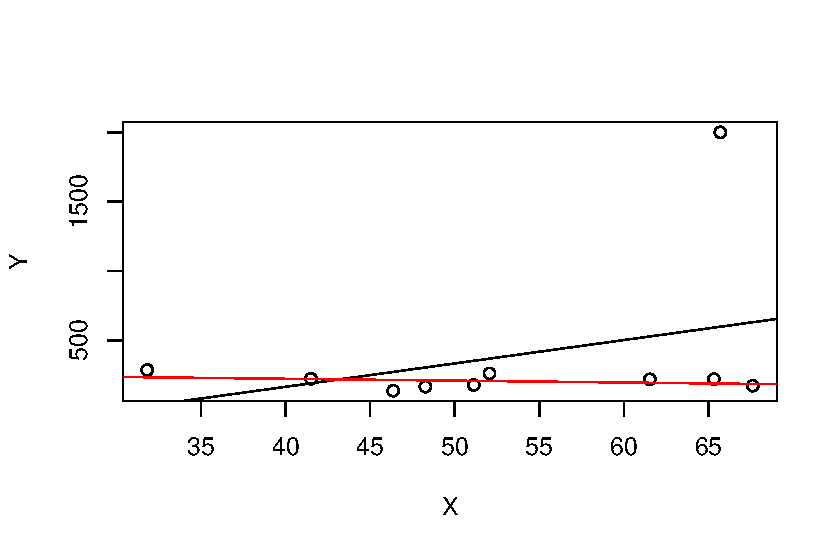
\includegraphics{ITER_files/figure-latex/unnamed-chunk-128-1} \end{center}

The plot shows positive correlation between age and earnings. This is in
line with the notion that older workers earn more than those who joined
the working population recently.

\subsubsection*{Sample Covariance and
Correlation}\label{sample-covariance-and-correlation}
\addcontentsline{toc}{subsubsection}{Sample Covariance and Correlation}

By now you should be familiar with the concepts of variance and
covariance. If not, we recommend you to work your way through Chapter 2
of the book.

Just like the variance, covariance and correlation of two variables are
properties that relate to the (unknown) joint probability distribution
of these variables. We can estimate covariance and correlation by means
of suitable estimators using a sample \((X_i,Y_i)\), \(i=1,\dots,n\).

The sample covariance

\[ s_{XY} = \frac{1}{n-1} \sum_{i=1}^n (X_i - \overline{X})(Y_i - \overline{Y}) \]

is an estimator for the population variance of \(X\) and \(Y\) whereas
the sample correlation

\[ r_{XY} = \frac{s_{XY}}{s_Xs_Y} \] can be used to estimate the
population correlation, a standardized measure for the strength of the
linear relationship between \(X\) and \(Y\). See Chapter 3.7 in the book
for a more detailed treatment of these estimators.

As for variance and standard deviation, these estimators are implemented
as \texttt{R} functions in the \texttt{stats} package. We can use them
to estimate population covariance and population correlation of the
artificial data on age and earnings.

\begin{Shaded}
\begin{Highlighting}[]
\CommentTok{# compute sample covariance of X and Y}
\KeywordTok{cov}\NormalTok{(X, Y)}
\end{Highlighting}
\end{Shaded}

\begin{verbatim}
## [1] 213.934
\end{verbatim}

\begin{Shaded}
\begin{Highlighting}[]
\CommentTok{# compute sample correlation between X and Y}
\KeywordTok{cor}\NormalTok{(X, Y)}
\end{Highlighting}
\end{Shaded}

\begin{verbatim}
## [1] 0.706372
\end{verbatim}

\begin{Shaded}
\begin{Highlighting}[]
\CommentTok{# an equivalent way to compute the sample correlation}
\KeywordTok{cov}\NormalTok{(X, Y) }\OperatorTok{/}\StringTok{ }\NormalTok{(}\KeywordTok{sd}\NormalTok{(X) }\OperatorTok{*}\StringTok{ }\KeywordTok{sd}\NormalTok{(Y))}
\end{Highlighting}
\end{Shaded}

\begin{verbatim}
## [1] 0.706372
\end{verbatim}

The estimates indicate that \(X\) and \(Y\) are moderately correlated.

The next code chunk uses the function \texttt{mvnorm()} from package
\texttt{MASS} \citep{R-MASS} to generate bivariate sample data with
different degrees of correlation.

\begin{Shaded}
\begin{Highlighting}[]
\KeywordTok{library}\NormalTok{(MASS)}

\CommentTok{# set random seed}
\KeywordTok{set.seed}\NormalTok{(}\DecValTok{1}\NormalTok{)}

\CommentTok{# positive correlation (0.81)}
\NormalTok{example1 <-}\StringTok{ }\KeywordTok{mvrnorm}\NormalTok{(}\DecValTok{100}\NormalTok{,}
                    \DataTypeTok{mu =} \KeywordTok{c}\NormalTok{(}\DecValTok{0}\NormalTok{, }\DecValTok{0}\NormalTok{), }
                    \DataTypeTok{Sigma =} \KeywordTok{matrix}\NormalTok{(}\KeywordTok{c}\NormalTok{(}\DecValTok{2}\NormalTok{, }\DecValTok{2}\NormalTok{, }\DecValTok{2}\NormalTok{, }\DecValTok{3}\NormalTok{), }\DataTypeTok{ncol =} \DecValTok{2}\NormalTok{),}
                    \DataTypeTok{empirical =} \OtherTok{TRUE}\NormalTok{)}

\CommentTok{# negative correlation (-0.81)}
\NormalTok{example2 <-}\StringTok{ }\KeywordTok{mvrnorm}\NormalTok{(}\DecValTok{100}\NormalTok{,}
                    \DataTypeTok{mu =} \KeywordTok{c}\NormalTok{(}\DecValTok{0}\NormalTok{, }\DecValTok{0}\NormalTok{), }
                    \DataTypeTok{Sigma =} \KeywordTok{matrix}\NormalTok{(}\KeywordTok{c}\NormalTok{(}\DecValTok{2}\NormalTok{, }\OperatorTok{-}\DecValTok{2}\NormalTok{, }\OperatorTok{-}\DecValTok{2}\NormalTok{, }\DecValTok{3}\NormalTok{), }\DataTypeTok{ncol =} \DecValTok{2}\NormalTok{),}
                    \DataTypeTok{empirical =} \OtherTok{TRUE}\NormalTok{)}

\CommentTok{# no correlation }
\NormalTok{example3 <-}\StringTok{ }\KeywordTok{mvrnorm}\NormalTok{(}\DecValTok{100}\NormalTok{,}
                    \DataTypeTok{mu =} \KeywordTok{c}\NormalTok{(}\DecValTok{0}\NormalTok{, }\DecValTok{0}\NormalTok{), }
                    \DataTypeTok{Sigma =} \KeywordTok{matrix}\NormalTok{(}\KeywordTok{c}\NormalTok{(}\DecValTok{1}\NormalTok{, }\DecValTok{0}\NormalTok{, }\DecValTok{0}\NormalTok{, }\DecValTok{1}\NormalTok{), }\DataTypeTok{ncol =} \DecValTok{2}\NormalTok{),}
                    \DataTypeTok{empirical =} \OtherTok{TRUE}\NormalTok{)}

\CommentTok{# no correlation (quadratic relationship)}
\NormalTok{X <-}\StringTok{ }\KeywordTok{seq}\NormalTok{(}\OperatorTok{-}\DecValTok{3}\NormalTok{, }\DecValTok{3}\NormalTok{, }\FloatTok{0.01}\NormalTok{)}
\NormalTok{Y <-}\StringTok{ }\OperatorTok{-}\StringTok{ }\NormalTok{X}\OperatorTok{^}\DecValTok{2} \OperatorTok{+}\StringTok{ }\KeywordTok{rnorm}\NormalTok{(}\KeywordTok{length}\NormalTok{(X))}

\NormalTok{example4 <-}\StringTok{ }\KeywordTok{cbind}\NormalTok{(X, Y)}

\CommentTok{# divide plot area as 2-by-2 array}
\KeywordTok{par}\NormalTok{(}\DataTypeTok{mfrow =} \KeywordTok{c}\NormalTok{(}\DecValTok{2}\NormalTok{, }\DecValTok{2}\NormalTok{))}

\CommentTok{# plot datasets}
\KeywordTok{plot}\NormalTok{(example1, }\DataTypeTok{col =} \StringTok{'steelblue'}\NormalTok{, }\DataTypeTok{pch =} \DecValTok{20}\NormalTok{, }\DataTypeTok{xlab =} \StringTok{'X'}\NormalTok{, }\DataTypeTok{ylab =} \StringTok{'Y'}\NormalTok{, }
     \DataTypeTok{main =} \StringTok{"Correlation = 0.81"}\NormalTok{)}

\KeywordTok{plot}\NormalTok{(example2, }\DataTypeTok{col =} \StringTok{'steelblue'}\NormalTok{, }\DataTypeTok{pch =} \DecValTok{20}\NormalTok{, }\DataTypeTok{xlab =} \StringTok{'X'}\NormalTok{, }\DataTypeTok{ylab =} \StringTok{'Y'}\NormalTok{, }
     \DataTypeTok{main =} \StringTok{"Correlation = -0.81"}\NormalTok{)}

\KeywordTok{plot}\NormalTok{(example3, }\DataTypeTok{col =} \StringTok{'steelblue'}\NormalTok{, }\DataTypeTok{pch =} \DecValTok{20}\NormalTok{, }\DataTypeTok{xlab =} \StringTok{'X'}\NormalTok{, }\DataTypeTok{ylab =} \StringTok{'Y'}\NormalTok{, }
     \DataTypeTok{main =} \StringTok{"Correlation = 0"}\NormalTok{)}

\KeywordTok{plot}\NormalTok{(example4, }\DataTypeTok{col =} \StringTok{'steelblue'}\NormalTok{, }\DataTypeTok{pch =} \DecValTok{20}\NormalTok{, }\DataTypeTok{xlab =} \StringTok{'X'}\NormalTok{, }\DataTypeTok{ylab =} \StringTok{'Y'}\NormalTok{, }
     \DataTypeTok{main =} \StringTok{"Correlation = 0"}\NormalTok{)}
\end{Highlighting}
\end{Shaded}

\begin{center}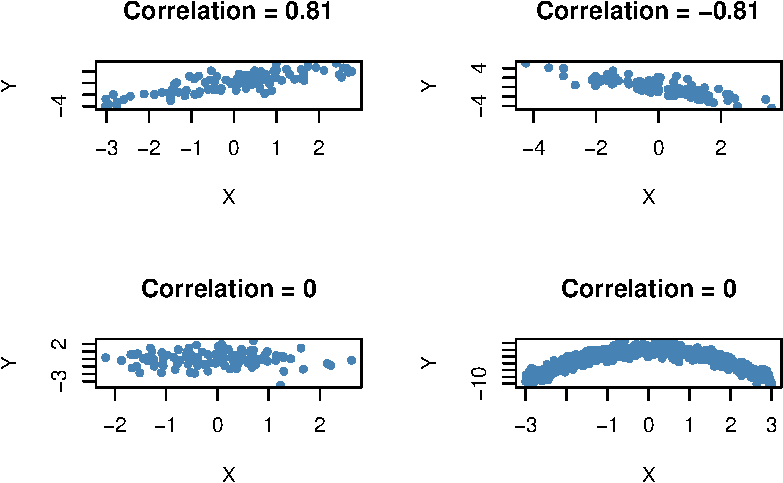
\includegraphics{ITER_files/figure-latex/unnamed-chunk-130-1} \end{center}

\section{Exercises}\label{exercises-1}

\begin{center}\textit{This interactive part of the book is only available in the HTML version.}\end{center}

\chapter{Linear Regression with One Regressor}\label{lrwor}

This chapter introduces the basics in linear regression and shows how to
perform regression analysis in \texttt{R}. In linear regression, the aim
is to model the relationship between a dependent variable \(Y\) and one
or more explanatory variables denoted by \(X_1, X_2, \dots, X_k\).
Following the book we will focus on the concept of simple linear
regression throughout the whole chapter. In simple linear regression,
there is just one explanatory variable \(X_1\). If, for example, a
school cuts its class sizes by hiring new teachers, that is, the school
lowers \(X_1\), the student-teacher ratios of its classes, how would
this affect \(Y\), the performance of the students involved in a
standardized test? With linear regression we can not only examine
whether the student-teacher ratio \emph{does have} an impact on the test
results but we can also learn about the \emph{direction} and the
\emph{strength} of this effect.

The following packages are needed for reproducing the code presented in
this chapter:

\begin{itemize}
\item
  \texttt{AER} - accompanies the Book \emph{Applied Econometrics with R}
  \citet{kleiber2008} and provides useful functions and data sets.
\item
  \texttt{MASS} - a collection of functions for applied statistics.
\end{itemize}

Make sure these are installed before you go ahead and try to replicate
the examples. The safest way to do so is by checking whether the
following code chunk executes without any errors.

\begin{Shaded}
\begin{Highlighting}[]
\KeywordTok{library}\NormalTok{(AER)}
\KeywordTok{library}\NormalTok{(MASS)}
\end{Highlighting}
\end{Shaded}

\section{Simple Linear Regression}\label{simple-linear-regression}

To start with an easy example, consider the following combinations of
average test score and the average student-teacher ratio in some
fictional school districts.

\begin{table}[H]
\centering
\begin{tabular}{lrrrrrrr}
\toprule
  & 1 & 2 & 3 & 4 & 5 & 6 & 7\\
\midrule
TestScore & 680 & 640 & 670 & 660 & 630 & 660.0 & 635\\
STR & 15 & 17 & 19 & 20 & 22 & 23.5 & 25\\
\bottomrule
\end{tabular}
\end{table}

To work with these data in \texttt{R} we begin by generating two
vectors: one for the student-teacher ratios (\texttt{STR}) and one for
test scores (\texttt{TestScore}), both containing the data from the
table above.

\begin{Shaded}
\begin{Highlighting}[]
\CommentTok{# Create sample data}
\NormalTok{STR <-}\StringTok{ }\KeywordTok{c}\NormalTok{(}\DecValTok{15}\NormalTok{, }\DecValTok{17}\NormalTok{, }\DecValTok{19}\NormalTok{, }\DecValTok{20}\NormalTok{, }\DecValTok{22}\NormalTok{, }\FloatTok{23.5}\NormalTok{, }\DecValTok{25}\NormalTok{)}
\NormalTok{TestScore <-}\StringTok{ }\KeywordTok{c}\NormalTok{(}\DecValTok{680}\NormalTok{, }\DecValTok{640}\NormalTok{, }\DecValTok{670}\NormalTok{, }\DecValTok{660}\NormalTok{, }\DecValTok{630}\NormalTok{, }\DecValTok{660}\NormalTok{, }\DecValTok{635}\NormalTok{) }

\CommentTok{# Print out sample data}
\NormalTok{STR}
\end{Highlighting}
\end{Shaded}

\begin{verbatim}
## [1] 15.0 17.0 19.0 20.0 22.0 23.5 25.0
\end{verbatim}

\begin{Shaded}
\begin{Highlighting}[]
\NormalTok{TestScore}
\end{Highlighting}
\end{Shaded}

\begin{verbatim}
## [1] 680 640 670 660 630 660 635
\end{verbatim}

In a simple linear regression model, we model the relationship between
both variables by a straight line, formally \[ Y = b \cdot X + a. \] For
now, let us suppose that the function which relates test score and
student-teacher ratio to each other is
\[TestScore = 713 - 3 \times STR.\]

It is always a good idea to visualize the data you work with. Here, it
is suitable to use \texttt{plot()} to produce a scatterplot with
\texttt{STR} on the \(x\)-axis and \texttt{TestScore} on the \(y\)-axis.
Just call \texttt{plot(y\_variable\ \textasciitilde{}\ x\_variable)}
whereby \texttt{y\_variable} and \texttt{x\_variable} are placeholders
for the vectors of observations we want to plot. Furthermore, we might
want to add a systematic relationship to the plot. To draw a straight
line, \texttt{R} provides the function \texttt{abline()}. We just have
to call this function with arguments \texttt{a} (representing the
intercept) and \texttt{b} (representing the slope) after executing
\texttt{plot()} in order to add the line to our plot.

The following code reproduces Figure 4.1 from the textbook.

\begin{Shaded}
\begin{Highlighting}[]
\CommentTok{# create a scatterplot of the data}
\KeywordTok{plot}\NormalTok{(TestScore }\OperatorTok{~}\StringTok{ }\NormalTok{STR)}

\CommentTok{# add the systematic relationship to the plot}
\KeywordTok{abline}\NormalTok{(}\DataTypeTok{a =} \DecValTok{713}\NormalTok{, }\DataTypeTok{b =} \OperatorTok{-}\DecValTok{3}\NormalTok{)}
\end{Highlighting}
\end{Shaded}

\begin{center}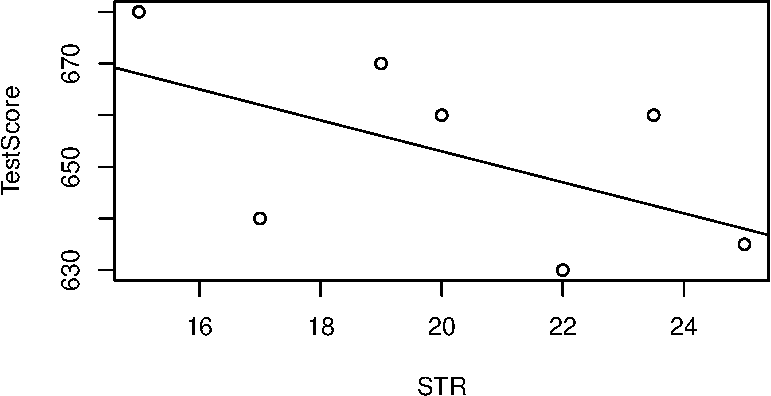
\includegraphics{ITER_files/figure-latex/unnamed-chunk-144-1} \end{center}

We find that the line does not touch any of the points although we
claimed that it represents the systematic relationship. The reason for
this is randomness. Most of the time there are additional influences
which imply that there is no bivariate relationship between the two
variables.

In order to account for these differences between observed data and the
systematic relationship, we extend our model from above by an
\emph{error term} \(u\) which captures additional random effects. Put
differently, \(u\) accounts for all the differences between the
regression line and the actual observed data. Beside pure randomness,
these deviations could also arise from measurement errors or, as will be
discussed later, could be the consequence of leaving out other factors
that are relevant in explaining the dependent variable.

Which other factors are plausible in our example? For one thing, the
test scores might be driven by the teachers' quality and the background
of the students. It is also possible that in some classes, the students
were lucky on the test days and thus achieved higher scores. For now, we
will summarize such influences by an additive component:

\[ TestScore = \beta_0 + \beta_1 \times STR + \text{other factors} \]

Of course this idea is very general as it can be easily extended to
other situations that can be described with a linear model. The basic
linear regression function we will work with hence is

\[ Y_i = \beta_0 + \beta_1 X_i + u_i. \]

Key Concept 4.1 summarizes the terminology of the simple linear
regression model.

\begin{keyconcepts}[Terminology for the Linear Regression Model with a Single Regressor]{4.1}
The linear regression model is $$Y_i = \beta_0 + \beta_1 X_1 + u_i$$
where
\begin{itemize}
\item the index $i$ runs over the observations, $i=1,\dots,n$
\item $Y_i$ is the \textit{dependent variable}, the \textit{regressand}, or simply the \textit{left-hand variable}
\item $X_i$ is the \textit{independent variable}, the \textit{regressor}, or simply the \textit{right-hand variable}
\item $Y = \beta_0 + \beta_1 X$ is the \textit{population regression line} also called the \textit{population regression function}
\item $\beta_0$ is the \textit{intercept} of the population regression line
\item $\beta_1$ is the \textit{slope} of the population regression line
\item $u_i$ is the \textit{error term}.
\end{itemize}
\end{keyconcepts}

\section{Estimating the Coefficients of the Linear Regression
Model}\label{estimating-the-coefficients-of-the-linear-regression-model}

In practice, the intercept \(\beta_0\) and slope \(\beta_1\) of the
population regression line are unknown. Therefore, we must employ data
to estimate both unknown parameters. In the following, a real world
example will be used to demonstrate how this is achieved. We want to
relate test scores to student-teacher ratios measured in Californian
schools. The test score is the district-wide average of reading and math
scores for fifth graders. Again, the class size is measured as the
number of students divided by the number of teachers (the
student-teacher ratio). As for the data, the California School data set
(\texttt{CASchools}) comes with an \texttt{R} package called
\texttt{AER}, an acronym for
\href{https://cran.r-project.org/web/packages/AER/AER.pdf}{Applied
Econometrics with R} \citep{R-AER}. After installing the package with
\texttt{install.packages("AER")} and attaching it with
\texttt{library(AER)} the data set can be loaded using the function
\texttt{data()}.

\begin{Shaded}
\begin{Highlighting}[]
\CommentTok{# install the AER package (once)}
\KeywordTok{install.packages}\NormalTok{(}\StringTok{"AER"}\NormalTok{)}

\CommentTok{# load the AER package }
\KeywordTok{library}\NormalTok{(AER)   }

\CommentTok{# load the the data set in the workspace}
\KeywordTok{data}\NormalTok{(CASchools) }
\end{Highlighting}
\end{Shaded}

Once a package has been installed it is available for use at further
occasions when invoked with \texttt{library()} --- there is no need to
run \texttt{install.packages()} again!

It is interesting to know what kind of object we are dealing with.
\texttt{class()} returns the class of an object. Depending on the class
of an object some functions (for example \texttt{plot()} and
\texttt{summary()}) behave differently.

Let us check the class of the object \texttt{CASchools}.

\begin{Shaded}
\begin{Highlighting}[]
\KeywordTok{class}\NormalTok{(CASchools)}
\end{Highlighting}
\end{Shaded}

\begin{verbatim}
## [1] "data.frame"
\end{verbatim}

It turns out that \texttt{CASchools} is of class \texttt{data.frame}
which is a convenient format to work with, especially for performing
regression analysis.

With help of \texttt{head()} we get a first overview of our data. This
function shows only the first 6 rows of the data set which prevents an
overcrowded console output.

\BeginKnitrBlock{rmdnote}
Press ctrl + L to clear the console. This command deletes any code that
has been typed in and executed by you or printed to the console by R
functions. The good news is that anything else is left untouched. You
neither loose defined variables etc. nor the code history. It is still
possible to recall previously executed R commands using the up and down
keys. If you are working in \emph{RStudio}, press ctrl + Up on your
keyboard (CMD + Up on a Mac) to review a list of previously entered
commands.
\EndKnitrBlock{rmdnote}

\begin{Shaded}
\begin{Highlighting}[]
\KeywordTok{head}\NormalTok{(CASchools)}
\end{Highlighting}
\end{Shaded}

\begin{verbatim}
##   district                          school  county grades students
## 1    75119              Sunol Glen Unified Alameda  KK-08      195
## 2    61499            Manzanita Elementary   Butte  KK-08      240
## 3    61549     Thermalito Union Elementary   Butte  KK-08     1550
## 4    61457 Golden Feather Union Elementary   Butte  KK-08      243
## 5    61523        Palermo Union Elementary   Butte  KK-08     1335
## 6    62042         Burrel Union Elementary  Fresno  KK-08      137
##   teachers calworks   lunch computer expenditure    income   english  read
## 1    10.90   0.5102  2.0408       67    6384.911 22.690001  0.000000 691.6
## 2    11.15  15.4167 47.9167      101    5099.381  9.824000  4.583333 660.5
## 3    82.90  55.0323 76.3226      169    5501.955  8.978000 30.000002 636.3
## 4    14.00  36.4754 77.0492       85    7101.831  8.978000  0.000000 651.9
## 5    71.50  33.1086 78.4270      171    5235.988  9.080333 13.857677 641.8
## 6     6.40  12.3188 86.9565       25    5580.147 10.415000 12.408759 605.7
##    math
## 1 690.0
## 2 661.9
## 3 650.9
## 4 643.5
## 5 639.9
## 6 605.4
\end{verbatim}

We find that the data set consists of plenty of variables and that most
of them are numeric.

By the way: an alternative to \texttt{class()} and \texttt{head()} is
\texttt{str()} which is deduced from `structure' and gives a
comprehensive overview of the object. Try!

Turning back to \texttt{CASchools}, the two variables we are interested
in (i.e., average test score and the student-teacher ratio) are
\emph{not} included. However, it is possible to calculate both from the
provided data. To obtain the student-teacher ratios, we simply divide
the number of students by the number of teachers. The average test score
is the arithmetic mean of the test score for reading and the score of
the math test. The next code chunk shows how the two variables can be
constructed as vectors and how they are appended to \texttt{CASchools}.

\begin{Shaded}
\begin{Highlighting}[]
\CommentTok{# compute STR and append it to CASchools}
\NormalTok{CASchools}\OperatorTok{$}\NormalTok{STR <-}\StringTok{ }\NormalTok{CASchools}\OperatorTok{$}\NormalTok{students}\OperatorTok{/}\NormalTok{CASchools}\OperatorTok{$}\NormalTok{teachers }

\CommentTok{# compute TestScore and append it to CASchools}
\NormalTok{CASchools}\OperatorTok{$}\NormalTok{score <-}\StringTok{ }\NormalTok{(CASchools}\OperatorTok{$}\NormalTok{read }\OperatorTok{+}\StringTok{ }\NormalTok{CASchools}\OperatorTok{$}\NormalTok{math)}\OperatorTok{/}\DecValTok{2}     
\end{Highlighting}
\end{Shaded}

If we ran \texttt{head(CASchools)} again we would find the two variables
of interest as additional columns named \texttt{STR} and \texttt{score}
(check this!).

Table 4.1 from the textbook summarizes the distribution of test scores
and student-teacher ratios. There are several functions which can be
used to produce similar results, e.g.,

\begin{itemize}
\item
  \texttt{mean()} (computes the arithmetic mean of the provided
  numbers),
\item
  \texttt{sd()} (computes the sample standard deviation),
\item
  \texttt{quantile()} (returns a vector of the specified sample
  quantiles for the data).
\end{itemize}

The next code chunk shows how to achieve this. First, we compute summary
statistics on the columns \texttt{STR} and \texttt{score} of
\texttt{CASchools}. In order to get nice output we gather the measures
in a \texttt{data.frame} named \texttt{DistributionSummary}.

\begin{Shaded}
\begin{Highlighting}[]
\CommentTok{# compute sample averages of STR and score}
\NormalTok{avg_STR <-}\StringTok{ }\KeywordTok{mean}\NormalTok{(CASchools}\OperatorTok{$}\NormalTok{STR) }
\NormalTok{avg_score <-}\StringTok{ }\KeywordTok{mean}\NormalTok{(CASchools}\OperatorTok{$}\NormalTok{score)}

\CommentTok{# compute sample standard deviations of STR and score}
\NormalTok{sd_STR <-}\StringTok{ }\KeywordTok{sd}\NormalTok{(CASchools}\OperatorTok{$}\NormalTok{STR) }
\NormalTok{sd_score <-}\StringTok{ }\KeywordTok{sd}\NormalTok{(CASchools}\OperatorTok{$}\NormalTok{score)}

\CommentTok{# set up a vector of percentiles and compute the quantiles }
\NormalTok{quantiles <-}\StringTok{ }\KeywordTok{c}\NormalTok{(}\FloatTok{0.10}\NormalTok{, }\FloatTok{0.25}\NormalTok{, }\FloatTok{0.4}\NormalTok{, }\FloatTok{0.5}\NormalTok{, }\FloatTok{0.6}\NormalTok{, }\FloatTok{0.75}\NormalTok{, }\FloatTok{0.9}\NormalTok{)}
\NormalTok{quant_STR <-}\StringTok{ }\KeywordTok{quantile}\NormalTok{(CASchools}\OperatorTok{$}\NormalTok{STR, quantiles)}
\NormalTok{quant_score <-}\StringTok{ }\KeywordTok{quantile}\NormalTok{(CASchools}\OperatorTok{$}\NormalTok{score, quantiles)}

\CommentTok{# gather everything in a data.frame }
\NormalTok{DistributionSummary <-}\StringTok{ }\KeywordTok{data.frame}\NormalTok{(}\DataTypeTok{Average =} \KeywordTok{c}\NormalTok{(avg_STR, avg_score), }
                                  \DataTypeTok{StandardDeviation =} \KeywordTok{c}\NormalTok{(sd_STR, sd_score), }
                                  \DataTypeTok{quantile =} \KeywordTok{rbind}\NormalTok{(quant_STR, quant_score))}

\CommentTok{# print the summary to the console}
\NormalTok{DistributionSummary}
\end{Highlighting}
\end{Shaded}

\begin{verbatim}
##               Average StandardDeviation quantile.10. quantile.25.
## quant_STR    19.64043          1.891812      17.3486     18.58236
## quant_score 654.15655         19.053347     630.3950    640.05000
##             quantile.40. quantile.50. quantile.60. quantile.75.
## quant_STR       19.26618     19.72321      20.0783     20.87181
## quant_score    649.06999    654.45000     659.4000    666.66249
##             quantile.90.
## quant_STR       21.86741
## quant_score    678.85999
\end{verbatim}

As for the sample data, we use \texttt{plot()}. This allows us to detect
characteristics of our data, such as outliers which are harder to
discover by looking at mere numbers. This time we add some additional
arguments to the call of \texttt{plot()}.

The first argument in our call of \texttt{plot()},
\texttt{score \textasciitilde{} STR}, is again a formula that states
variables on the y- and the x-axis. However, this time the two variables
are not saved in separate vectors but are columns of \texttt{CASchools}.
Therefore, \texttt{R} would not find them without the argument
\texttt{data} being correctly specified. \texttt{data} must be in
accordance with the name of the \texttt{data.frame} to which the
variables belong to, in this case \texttt{CASchools}. Further arguments
are used to change the appearance of the plot: while \texttt{main} adds
a title, \texttt{xlab} and \texttt{ylab} add custom labels to both axes.

\begin{Shaded}
\begin{Highlighting}[]
\KeywordTok{plot}\NormalTok{(score }\OperatorTok{~}\StringTok{ }\NormalTok{STR, }
     \DataTypeTok{data =}\NormalTok{ CASchools,}
     \DataTypeTok{main =} \StringTok{"Scatterplot of TestScore and STR"}\NormalTok{, }
     \DataTypeTok{xlab =} \StringTok{"STR (X)"}\NormalTok{,}
     \DataTypeTok{ylab =} \StringTok{"Test Score (Y)"}\NormalTok{)}
\end{Highlighting}
\end{Shaded}

\begin{center}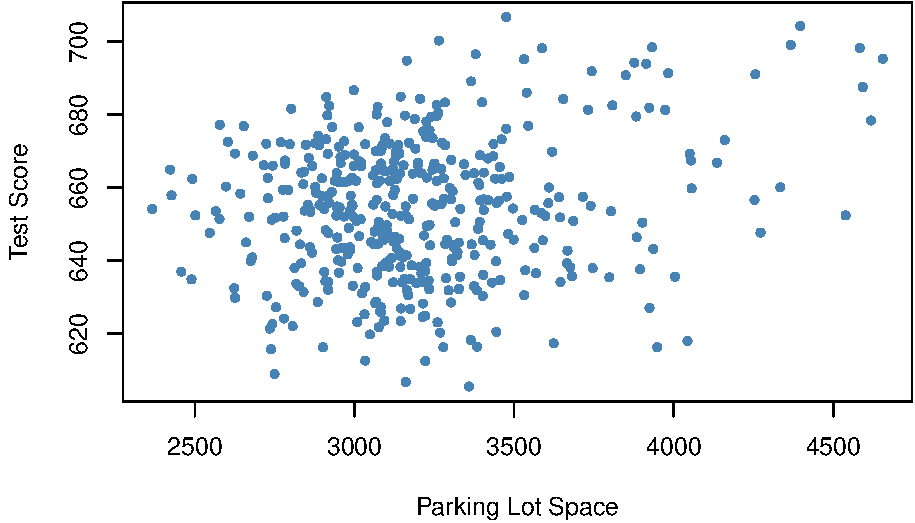
\includegraphics{ITER_files/figure-latex/unnamed-chunk-152-1} \end{center}

The plot (Figure 4.2 in the book) shows the scatterplot of all
observations on the student-teacher ratio and test score. We see that
the points are strongly scattered, and that the variables are negatively
correlated. That is, we expect to observe lower test scores in bigger
classes.

The function \texttt{cor()} (see \texttt{?cor} for further info) can be
used to compute the correlation between two \emph{numeric} vectors.

\begin{Shaded}
\begin{Highlighting}[]
\KeywordTok{cor}\NormalTok{(CASchools}\OperatorTok{$}\NormalTok{STR, CASchools}\OperatorTok{$}\NormalTok{score)}
\end{Highlighting}
\end{Shaded}

\begin{verbatim}
## [1] -0.2263627
\end{verbatim}

As the scatterplot already suggests, the correlation is negative but
rather weak.

The task we are now facing is to find a line which best fits the data.
Of course we could simply stick with graphical inspection and
correlation analysis and then select the best fitting line by
eyeballing. However, this would be rather subjective: different
observers would draw different regression lines. On this account, we are
interested in techniques that are less arbitrary. Such a technique is
given by ordinary least squares (OLS) estimation.

\subsection*{The Ordinary Least Squares
Estimator}\label{the-ordinary-least-squares-estimator}
\addcontentsline{toc}{subsection}{The Ordinary Least Squares Estimator}

The OLS estimator chooses the regression coefficients such that the
estimated regression line is as ``close'' as possible to the observed
data points. Here, closeness is measured by the sum of the squared
mistakes made in predicting \(Y\) given \(X\). Let \(b_0\) and \(b_1\)
be some estimators of \(\beta_0\) and \(\beta_1\). Then the sum of
squared estimation mistakes can be expressed as

\[ \sum^n_{i = 1} (Y_i - b_0 - b_1 X_i)^2. \]

The OLS estimator in the simple regression model is the pair of
estimators for intercept and slope which minimizes the expression above.
The derivation of the OLS estimators for both parameters are presented
in Appendix 4.1 of the book. The results are summarized in Key Concept
4.2.

\begin{keyconcepts}[The OLS Estimator, Predicted Values, and Residuals]{4.2}
The OLS estimators of the slope $\beta_1$ and the intercept $\beta_0$ in the simple linear regression model are
\begin{align*}
  \hat\beta_1 & = \frac{ \sum_{i = 1}^n (X_i - \overline{X})(Y_i - \overline{Y}) } { \sum_{i=1}^n (X_i - \overline{X})^2},  \\
\hat\beta_0 & =  \overline{Y} - \hat\beta_1 \overline{X}. 
\intertext{The OLS predicted values $\widehat{Y}_i$ and residuals $\hat{u}_i$ are}
  \widehat{Y}_i & =  \hat\beta_0 + \hat\beta_1 X_i,\\
  \hat{u}_i & =  Y_i - \widehat{Y}_i. 
\end{align*}

The estimated intercept $\hat{\beta}_0$, the slope parameter $\hat{\beta}_1$ and the residuals $\left(\hat{u}_i\right)$ are computed from a sample of $n$ observations of $X_i$ and $Y_i$, $i$, $...$,  $n$. These are \textit{estimates} of the unknown true population intercept $\left(\beta_0 \right)$, slope $\left(\beta_1\right)$, and error term $(u_i)$.
\end{keyconcepts}

There are many possible ways to compute \(\hat{\beta}_0\) and
\(\hat{\beta}_1\) in \texttt{R}. For example, we could implement the
formulas presented in Key Concept 4.2 with two of \texttt{R}'s most
basic functions: \texttt{mean()} and \texttt{sum()}.

\begin{Shaded}
\begin{Highlighting}[]
\KeywordTok{attach}\NormalTok{(CASchools) }\CommentTok{# allows to use the variables contained in CASchools directly}

\CommentTok{# compute beta_1_hat}
\NormalTok{beta_}\DecValTok{1}\NormalTok{ <-}\StringTok{ }\KeywordTok{sum}\NormalTok{((STR }\OperatorTok{-}\StringTok{ }\KeywordTok{mean}\NormalTok{(STR)) }\OperatorTok{*}\StringTok{ }\NormalTok{(score }\OperatorTok{-}\StringTok{ }\KeywordTok{mean}\NormalTok{(score))) }\OperatorTok{/}\StringTok{ }\KeywordTok{sum}\NormalTok{((STR }\OperatorTok{-}\StringTok{ }\KeywordTok{mean}\NormalTok{(STR))}\OperatorTok{^}\DecValTok{2}\NormalTok{)}

\CommentTok{# compute beta_0_hat}
\NormalTok{beta_}\DecValTok{0}\NormalTok{ <-}\StringTok{ }\KeywordTok{mean}\NormalTok{(score) }\OperatorTok{-}\StringTok{ }\NormalTok{beta_}\DecValTok{1} \OperatorTok{*}\StringTok{ }\KeywordTok{mean}\NormalTok{(STR)}

\CommentTok{# print the results to the console}
\NormalTok{beta_}\DecValTok{1}
\end{Highlighting}
\end{Shaded}

\begin{verbatim}
## [1] -2.279808
\end{verbatim}

\begin{Shaded}
\begin{Highlighting}[]
\NormalTok{beta_}\DecValTok{0}
\end{Highlighting}
\end{Shaded}

\begin{verbatim}
## [1] 698.9329
\end{verbatim}

Of course, there are even more manual ways to perform these tasks. With
OLS being one of the most widely-used estimation techniques, \texttt{R}
of course already contains a built-in function named \texttt{lm()}
(\textbf{l}inear \textbf{m}odel) which can be used to carry out
regression analysis.

The first argument of the function to be specified is, similar to
\texttt{plot()}, the regression formula with the basic syntax
\texttt{y \textasciitilde{} x} where \texttt{y} is the dependent
variable and \texttt{x} the explanatory variable. The argument
\texttt{data} determines the data set to be used in the regression. We
now revisit the example from the book where the relationship between the
test scores and the class sizes is analyzed. The following code uses
\texttt{lm()} to replicate the results presented in figure 4.3 of the
book.

\begin{Shaded}
\begin{Highlighting}[]
\CommentTok{# estimate the model and assign the result to linear_model}
\NormalTok{linear_model <-}\StringTok{ }\KeywordTok{lm}\NormalTok{(score }\OperatorTok{~}\StringTok{ }\NormalTok{STR, }\DataTypeTok{data =}\NormalTok{ CASchools)}

\CommentTok{# print the standard output of the estimated lm object to the console }
\NormalTok{linear_model}
\end{Highlighting}
\end{Shaded}

\begin{verbatim}
## 
## Call:
## lm(formula = score ~ STR, data = CASchools)
## 
## Coefficients:
## (Intercept)          STR  
##      698.93        -2.28
\end{verbatim}

Let us add the estimated regression line to the plot. This time we also
enlarge the ranges of both axes by setting the arguments \texttt{xlim}
and \texttt{ylim}.

\begin{Shaded}
\begin{Highlighting}[]
\CommentTok{# plot the data}
\KeywordTok{plot}\NormalTok{(score }\OperatorTok{~}\StringTok{ }\NormalTok{STR, }
     \DataTypeTok{data =}\NormalTok{ CASchools,}
     \DataTypeTok{main =} \StringTok{"Scatterplot of TestScore and STR"}\NormalTok{, }
     \DataTypeTok{xlab =} \StringTok{"STR (X)"}\NormalTok{,}
     \DataTypeTok{ylab =} \StringTok{"Test Score (Y)"}\NormalTok{,}
     \DataTypeTok{xlim =} \KeywordTok{c}\NormalTok{(}\DecValTok{10}\NormalTok{, }\DecValTok{30}\NormalTok{),}
     \DataTypeTok{ylim =} \KeywordTok{c}\NormalTok{(}\DecValTok{600}\NormalTok{, }\DecValTok{720}\NormalTok{))}

\CommentTok{# add the regression line}
\KeywordTok{abline}\NormalTok{(linear_model) }
\end{Highlighting}
\end{Shaded}

\begin{center}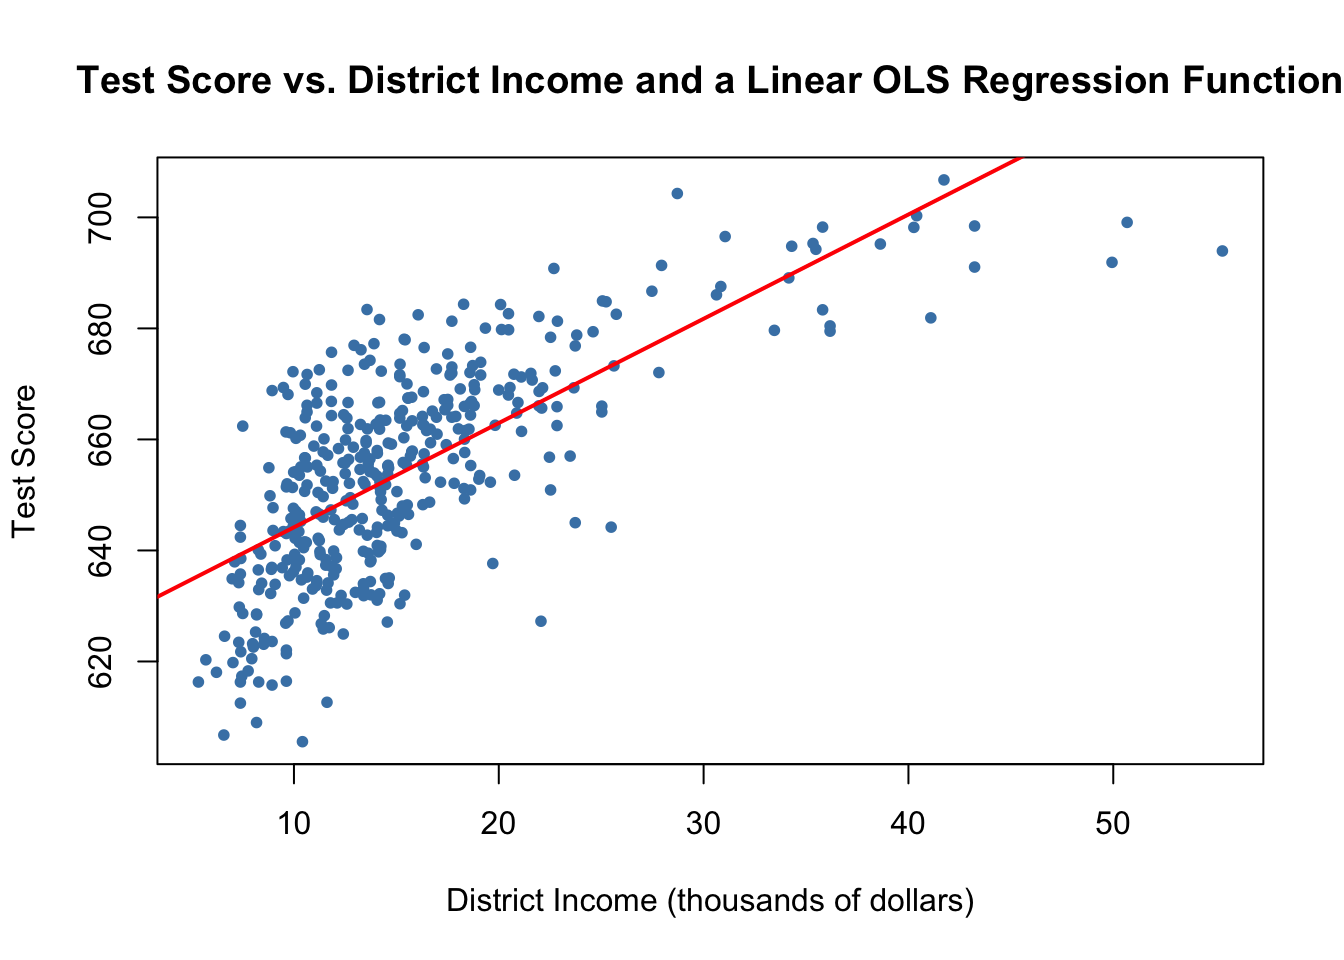
\includegraphics{ITER_files/figure-latex/unnamed-chunk-158-1} \end{center}

Did you notice that this time, we did not pass the intercept and slope
parameters to \texttt{abline}? If you call \texttt{abline()} on an
object of class \texttt{lm} that only contains a single regressor,
\texttt{R} draws the regression line automatically!

\section{Measures of Fit}\label{measures-of-fit}

After fitting a linear regression model, a natural question is how well
the model describes the data. Visually, this amounts to assessing
whether the observations are tightly clustered around the regression
line. Both the \emph{coefficient of determination} and the
\emph{standard error of the regression} measure how well the OLS
Regression line fits the data.

\subsection*{The Coefficient of
Determination}\label{the-coefficient-of-determination}
\addcontentsline{toc}{subsection}{The Coefficient of Determination}

\(R^2\), the \emph{coefficient of determination}, is the fraction of the
sample variance of \(Y_i\) that is explained by \(X_i\). Mathematically,
the \(R^2\) can be written as the ratio of the explained sum of squares
to the total sum of squares. The \emph{explained sum of squares}
(\(ESS\)) is the sum of squared deviations of the predicted values
\(\hat{Y_i}\), from the average of the \(Y_i\). The \emph{total sum of
squares} (\(TSS\)) is the sum of squared deviations of the \(Y_i\) from
their average. Thus we have

\begin{align}
  ESS & =  \sum_{i = 1}^n \left( \hat{Y_i} - \overline{Y} \right)^2,   \\
  TSS & =  \sum_{i = 1}^n \left( Y_i - \overline{Y} \right)^2,   \\
  R^2 & = \frac{ESS}{TSS}.
\end{align}

Since \(TSS = ESS + SSR\) we can also write

\[ R^2 = 1- \frac{SSR}{TSS} \]

where \(SSR\) is the sum of squared residuals, a measure for the errors
made when predicting the \(Y\) by \(X\). The \(SSR\) is defined as

\[ SSR = \sum_{i=1}^n \hat{u}_i^2. \]

\(R^2\) lies between \(0\) and \(1\). It is easy to see that a perfect
fit, i.e., no errors made when fitting the regression line, implies
\(R^2 = 1\) since then we have \(SSR=0\). On the contrary, if our
estimated regression line does not explain any variation in the \(Y_i\),
we have \(ESS=0\) and consequently \(R^2=0\).

\subsection*{The Standard Error of the
Regression}\label{the-standard-error-of-the-regression}
\addcontentsline{toc}{subsection}{The Standard Error of the Regression}

The \emph{Standard Error of the Regression} (\(SER\)) is an estimator of
the standard deviation of the residuals \(\hat{u}_i\). As such it
measures the magnitude of a typical deviation from the regression line,
i.e., the magnitude of a typical residual.

\[ SER = s_{\hat{u}} = \sqrt{s_{\hat{u}}^2} \ \ \ \text{where} \ \ \ s_{\hat{u} }^2 = \frac{1}{n-2} \sum_{i = 1}^n \hat{u}^2_i = \frac{SSR}{n - 2} \]

Remember that the \(u_i\) are \emph{unobserved}. This is why we use
their estimated counterparts, the residuals \(\hat{u}_i\), instead. See
Chapter 4.3 of the book for a more detailed comment on the \(SER\).

\subsection*{Application to the Test Score
Data}\label{application-to-the-test-score-data}
\addcontentsline{toc}{subsection}{Application to the Test Score Data}

Both measures of fit can be obtained by using the function
\texttt{summary()} with an \texttt{lm} object provided as the only
argument. While the function \texttt{lm()} only prints out the estimated
coefficients to the console, \texttt{summary()} provides additional
predefined information such as the regression's \(R^2\) and the \(SER\).

\begin{Shaded}
\begin{Highlighting}[]
\NormalTok{mod_summary <-}\StringTok{ }\KeywordTok{summary}\NormalTok{(linear_model)}
\NormalTok{mod_summary}
\end{Highlighting}
\end{Shaded}

\begin{verbatim}
## 
## Call:
## lm(formula = score ~ STR, data = CASchools)
## 
## Residuals:
##     Min      1Q  Median      3Q     Max 
## -47.727 -14.251   0.483  12.822  48.540 
## 
## Coefficients:
##             Estimate Std. Error t value Pr(>|t|)    
## (Intercept) 698.9329     9.4675  73.825  < 2e-16 ***
## STR          -2.2798     0.4798  -4.751 2.78e-06 ***
## ---
## Signif. codes:  0 '***' 0.001 '**' 0.01 '*' 0.05 '.' 0.1 ' ' 1
## 
## Residual standard error: 18.58 on 418 degrees of freedom
## Multiple R-squared:  0.05124,    Adjusted R-squared:  0.04897 
## F-statistic: 22.58 on 1 and 418 DF,  p-value: 2.783e-06
\end{verbatim}

The \(R^2\) in the output is called \emph{Multiple R-squared} and has a
value of \(0.051\). Hence, \(5.1 \%\) of the variance of the dependent
variable \(score\) is explained by the explanatory variable \(STR\).
That is, the regression explains little of the variance in \(score\),
and much of the variation in test scores remains unexplained (cf.~Figure
4.3 of the book).

The \(SER\) is called \emph{Residual standard error} and equals
\(18.58\). The unit of the \(SER\) is the same as the unit of the
dependent variable. That is, on average the deviation of the actual
achieved test score and the regression line is \(18.58\) points.

Now, let us check whether \texttt{summary()} uses the same definitions
for \(R^2\) and \(SER\) as we do when computing them manually.

\begin{Shaded}
\begin{Highlighting}[]
\CommentTok{# compute R^2 manually}
\NormalTok{SSR <-}\StringTok{ }\KeywordTok{sum}\NormalTok{(mod_summary}\OperatorTok{$}\NormalTok{residuals}\OperatorTok{^}\DecValTok{2}\NormalTok{)}
\NormalTok{TSS <-}\StringTok{ }\KeywordTok{sum}\NormalTok{((score }\OperatorTok{-}\StringTok{ }\KeywordTok{mean}\NormalTok{(score))}\OperatorTok{^}\DecValTok{2}\NormalTok{)}
\NormalTok{R2 <-}\StringTok{ }\DecValTok{1} \OperatorTok{-}\StringTok{ }\NormalTok{SSR}\OperatorTok{/}\NormalTok{TSS}

\CommentTok{# print the value to the console}
\NormalTok{R2}
\end{Highlighting}
\end{Shaded}

\begin{verbatim}
## [1] 0.05124009
\end{verbatim}

\begin{Shaded}
\begin{Highlighting}[]
\CommentTok{# compute SER manually}
\NormalTok{n <-}\StringTok{ }\KeywordTok{nrow}\NormalTok{(CASchools)}
\NormalTok{SER <-}\StringTok{ }\KeywordTok{sqrt}\NormalTok{(SSR }\OperatorTok{/}\StringTok{ }\NormalTok{(n}\OperatorTok{-}\DecValTok{2}\NormalTok{))}

\CommentTok{# print the value to the console}
\NormalTok{SER}
\end{Highlighting}
\end{Shaded}

\begin{verbatim}
## [1] 18.58097
\end{verbatim}

We find that the results coincide. Note that the values provided by
\texttt{summary()} are rounded to two decimal places. Can you do so
using \texttt{R}?

\section{The Least Squares Assumptions}\label{tlsa}

OLS performs well under a quite broad variety of different
circumstances. However, there are some assumptions which need to be
satisfied in order to ensure that the estimates are normally distributed
in large samples (we discuss this in Chapter @ref\{tsdotoe\}).

\begin{keyconcepts}[The Least Squares Assumptions]{4.3}
$$Y_i = \beta_0 + \beta_1 X_i + u_i \text{, } i = 1,\dots,n$$
where

\begin{enumerate}
\item The error term $u_i$ has conditional mean zero given $X_i$: $E(u_i|X_i) = 0$.
\item $(X_i,Y_i), i = 1,\dots,n$ are independent and identically distributed (i.i.d.) draws from their joint distribution.
\item Large outliers are unlikely: $X_i$ and $Y_i$ have nonzero finite fourth moments.
\end{enumerate}
\end{keyconcepts}

\subsection*{Assumption 1: The Error Term has Conditional Mean of
Zero}\label{assumption-1-the-error-term-has-conditional-mean-of-zero}
\addcontentsline{toc}{subsection}{Assumption 1: The Error Term has
Conditional Mean of Zero}

This means that no matter which value we choose for \(X\), the error
term \(u\) must not show any systematic pattern and must have a mean of
\(0\). Consider the case that, unconditionally, \(E(u) = 0\), but for
low and high values of \(X\), the error term tends to be positive and
for midrange values of \(X\) the error tends to be negative. We can use
R to construct such an example. To do so we generate our own data using
\texttt{R}'s built-in random number generators.

We will use the following functions:

\begin{itemize}
\tightlist
\item
  \texttt{runif()} - generates uniformly distributed random numbers
\item
  \texttt{rnorm()} - generates normally distributed random numbers
\item
  \texttt{predict()} - does predictions based on the results of model
  fitting functions like \texttt{lm()}
\item
  \texttt{lines()} - adds line segments to an existing plot
\end{itemize}

We start by creating a vector containing values that are uniformly
distributed on the interval \([-5,5]\). This can be done with the
function \texttt{runif()}. We also need to simulate the error term. For
this we generate normally distributed random numbers with a mean equal
to \(0\) and a variance of \(1\) using \texttt{rnorm()}. The \(Y\)
values are obtained as a quadratic function of the \(X\) values and the
error.

After generating the data we estimate both a simple regression model and
a quadratic model that also includes the regressor \(X^2\) (this is a
multiple regression model, see Chapter \ref{rmwmr}). Finally, we plot
the simulated data and add a the estimated regression line of a simple
regression model as well as the predictions made with a quadratic model
to compare the fit graphically.

\begin{Shaded}
\begin{Highlighting}[]
\CommentTok{# set a seed to make the results reproducible}
\KeywordTok{set.seed}\NormalTok{(}\DecValTok{321}\NormalTok{)}

\CommentTok{# simulate the data }
\NormalTok{X <-}\StringTok{ }\KeywordTok{runif}\NormalTok{(}\DecValTok{50}\NormalTok{, }\DataTypeTok{min =} \OperatorTok{-}\DecValTok{5}\NormalTok{, }\DataTypeTok{max =} \DecValTok{5}\NormalTok{)}
\NormalTok{u <-}\StringTok{ }\KeywordTok{rnorm}\NormalTok{(}\DecValTok{50}\NormalTok{, }\DataTypeTok{sd =} \DecValTok{5}\NormalTok{)  }

\CommentTok{# the true relation  }
\NormalTok{Y <-}\StringTok{ }\NormalTok{X}\OperatorTok{^}\DecValTok{2} \OperatorTok{+}\StringTok{ }\DecValTok{2} \OperatorTok{*}\StringTok{ }\NormalTok{X }\OperatorTok{+}\StringTok{ }\NormalTok{u                }

\CommentTok{# estimate a simple regression model }
\NormalTok{mod_simple <-}\StringTok{ }\KeywordTok{lm}\NormalTok{(Y }\OperatorTok{~}\StringTok{ }\NormalTok{X)}

\CommentTok{# predict using a quadratic model }
\NormalTok{prediction <-}\StringTok{ }\KeywordTok{predict}\NormalTok{(}\KeywordTok{lm}\NormalTok{(Y }\OperatorTok{~}\StringTok{ }\NormalTok{X }\OperatorTok{+}\StringTok{ }\KeywordTok{I}\NormalTok{(X}\OperatorTok{^}\DecValTok{2}\NormalTok{)), }\KeywordTok{data.frame}\NormalTok{(}\DataTypeTok{X =} \KeywordTok{sort}\NormalTok{(X)))}

\CommentTok{# plot the results}
\KeywordTok{plot}\NormalTok{(Y }\OperatorTok{~}\StringTok{ }\NormalTok{X)}
\KeywordTok{abline}\NormalTok{(mod_simple, }\DataTypeTok{col =} \StringTok{"red"}\NormalTok{)}
\KeywordTok{lines}\NormalTok{(}\KeywordTok{sort}\NormalTok{(X), prediction)}
\end{Highlighting}
\end{Shaded}

\begin{center}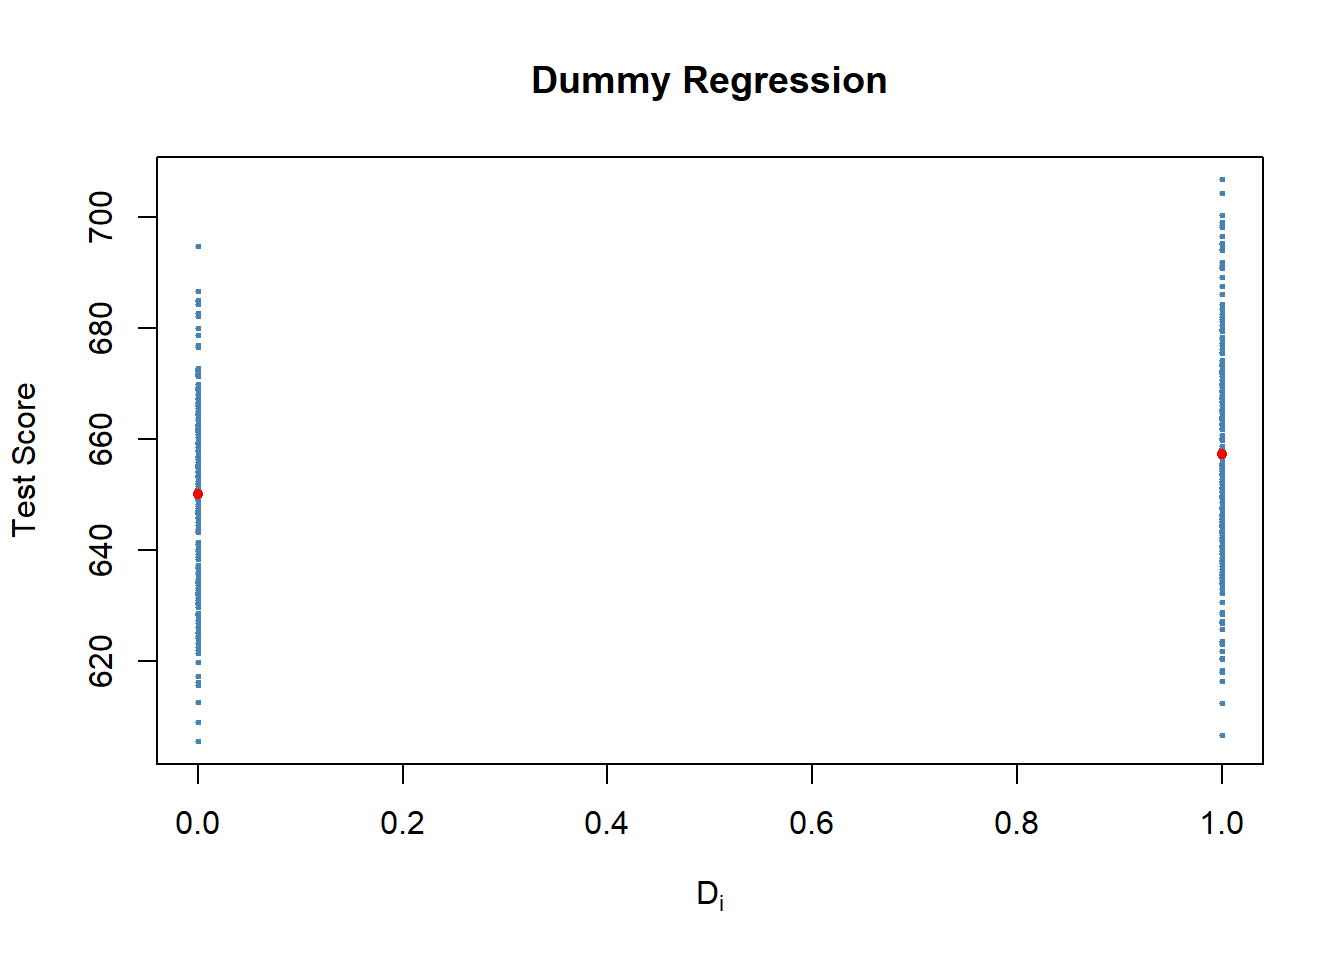
\includegraphics{ITER_files/figure-latex/unnamed-chunk-163-1} \end{center}

The plot shows what is meant by \(E(u_i|X_i) = 0\) and why it does not
hold for the linear model:

Using the quadratic model (represented by the black curve) we see that
there are no systematic deviations of the observation from the predicted
relation. It is credible that the assumption is not violated when such a
model is employed. However, using a simple linear regression model we
see that the assumption is probably violated as \(E(u_i|X_i)\) varies
with the \(X_i\).

\subsection*{Assumption 2: Independently and Identically Distributed
Data}\label{assumption-2-independently-and-identically-distributed-data}
\addcontentsline{toc}{subsection}{Assumption 2: Independently and
Identically Distributed Data}

Most sampling schemes used when collecting data from populations produce
i.i.d.-samples. For example, we could use \texttt{R}'s random number
generator to randomly select student IDs from a university's enrollment
list and record age \(X\) and earnings \(Y\) of the corresponding
students. This is a typical example of simple random sampling and
ensures that all the \((X_i, Y_i)\) are drawn randomly from the same
population.

A prominent example where the i.i.d. assumption is not fulfilled is time
series data where we have observations on the same unit over time. For
example, take \(X\) as the number of workers in a production company
over time. Due to business transformations, the company cuts job
periodically by a specific share but there are also some
non-deterministic influences that relate to economics, politics etc.
Using \texttt{R} we can easily simulate such a process and plot it.

We start the series with a total of 5000 workers and simulate the
reduction of employment with an autoregressive process that exhibits a
downward movement in the long-run and has normally distributed
errors:\footnote{See Chapter \ref{ittsraf} for more on autoregressive
  processes and time series analysis in general.}

\[ employment_t = -5 + 0.98 \cdot employment_{t-1} + u_t \]

\begin{Shaded}
\begin{Highlighting}[]
\CommentTok{# set seed}
\KeywordTok{set.seed}\NormalTok{(}\DecValTok{123}\NormalTok{)}

\CommentTok{# generate a date vector}
\NormalTok{Date <-}\StringTok{ }\KeywordTok{seq}\NormalTok{(}\KeywordTok{as.Date}\NormalTok{(}\StringTok{"1951/1/1"}\NormalTok{), }\KeywordTok{as.Date}\NormalTok{(}\StringTok{"2000/1/1"}\NormalTok{), }\StringTok{"years"}\NormalTok{)}

\CommentTok{# initialize the employment vector}
\NormalTok{X <-}\StringTok{ }\KeywordTok{c}\NormalTok{(}\DecValTok{5000}\NormalTok{, }\KeywordTok{rep}\NormalTok{(}\OtherTok{NA}\NormalTok{, }\KeywordTok{length}\NormalTok{(Date)}\OperatorTok{-}\DecValTok{1}\NormalTok{))}

\CommentTok{# generate time series observations with random influences}
\ControlFlowTok{for}\NormalTok{ (i }\ControlFlowTok{in} \DecValTok{2}\OperatorTok{:}\KeywordTok{length}\NormalTok{(Date)) \{}
  
\NormalTok{    X[i] <-}\StringTok{ }\OperatorTok{-}\DecValTok{50} \OperatorTok{+}\StringTok{ }\FloatTok{0.98} \OperatorTok{*}\StringTok{ }\NormalTok{X[i}\OperatorTok{-}\DecValTok{1}\NormalTok{] }\OperatorTok{+}\StringTok{ }\KeywordTok{rnorm}\NormalTok{(}\DataTypeTok{n =} \DecValTok{1}\NormalTok{, }\DataTypeTok{sd =} \DecValTok{200}\NormalTok{)}
    
\NormalTok{\}}

\CommentTok{#plot the results}
\KeywordTok{plot}\NormalTok{(}\DataTypeTok{x =}\NormalTok{ Date, }
     \DataTypeTok{y =}\NormalTok{ X, }
     \DataTypeTok{type =} \StringTok{"l"}\NormalTok{, }
     \DataTypeTok{col =} \StringTok{"steelblue"}\NormalTok{, }
     \DataTypeTok{ylab =} \StringTok{"Workers"}\NormalTok{, }
     \DataTypeTok{xlab =} \StringTok{"Time"}\NormalTok{)}
\end{Highlighting}
\end{Shaded}

\begin{center}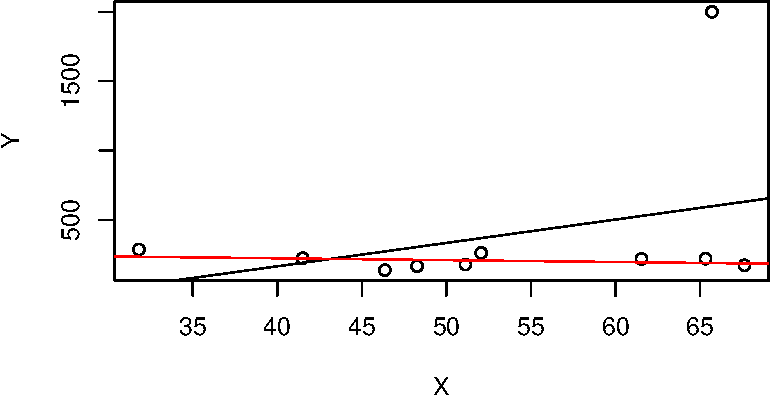
\includegraphics{ITER_files/figure-latex/unnamed-chunk-164-1} \end{center}

It is evident that the observations on the number of employees cannot be
independent in this example: the level of today's employment is
correlated with tomorrows employment level. Thus, the i.i.d. assumption
is violated.

\subsection*{Assumption 3: Large Outliers are
Unlikely}\label{assumption-3-large-outliers-are-unlikely}
\addcontentsline{toc}{subsection}{Assumption 3: Large Outliers are
Unlikely}

It is easy to come up with situations where extreme observations, i.e.,
observations that deviate considerably from the usual range of the data,
may occur. Such observations are called outliers. Technically speaking,
assumption 3 requires that \(X\) and \(Y\) have a finite
kurtosis.\footnote{See Chapter 4.4 of the book.}

Common cases where we want to exclude or (if possible) correct such
outliers is when they are apparently typos, conversion errors or
measurement errors. Even if it seems like extreme observations have been
recorded correctly, it is advisable to exclude them before estimating a
model since OLS suffers from \emph{sensitivity to outliers}.

What does this mean? One can show that extreme observations receive
heavy weighting in the estimation of the unknown regression coefficients
when using OLS. Therefore, outliers can lead to strongly distorted
estimates of regression coefficients. To get a better impression of this
issue, consider the following application where we have placed some
sample data on \(X\) and \(Y\) which are highly correlated. The relation
between \(X\) and \(Y\) seems to be explained pretty good by the plotted
regression line: all of the blue dots lie close to the red line and we
have \(R^2=0.92\).

Now go ahead and add a further observation at, say, \((18,2)\). This
observations clearly is an outlier. The result is quite striking: the
estimated regression line differs greatly from the one we adjudged to
fit the data well. The slope is heavily downward biased and \(R^2\)
decreased to a mere \(29\%\)! Double-click inside the coordinate system
to reset the app. Feel free to experiment. Choose different coordinates
for the outlier or add additional ones.

The following code roughly reproduces what is shown in figure 4.5 in the
book. As done above we use sample data generated using \texttt{R}'s
random number functions \texttt{rnorm()} and \texttt{runif()}. We
estimate two simple regression models, one based on the original data
set and another using a modified set where one observation is change to
be an outlier and then plot the results. In order to understand the
complete code you should be familiar with the function \texttt{sort()}
which sorts the entries of a numeric vector in ascending order.

\begin{Shaded}
\begin{Highlighting}[]
\CommentTok{# set seed}
\KeywordTok{set.seed}\NormalTok{(}\DecValTok{123}\NormalTok{)}

\CommentTok{# generate the data}
\NormalTok{X <-}\StringTok{ }\KeywordTok{sort}\NormalTok{(}\KeywordTok{runif}\NormalTok{(}\DecValTok{10}\NormalTok{, }\DataTypeTok{min =} \DecValTok{30}\NormalTok{, }\DataTypeTok{max =} \DecValTok{70}\NormalTok{))}
\NormalTok{Y <-}\StringTok{ }\KeywordTok{rnorm}\NormalTok{(}\DecValTok{10}\NormalTok{ , }\DataTypeTok{mean =} \DecValTok{200}\NormalTok{, }\DataTypeTok{sd =} \DecValTok{50}\NormalTok{)}
\NormalTok{Y[}\DecValTok{9}\NormalTok{] <-}\StringTok{ }\DecValTok{2000}

\CommentTok{# fit model with outlier}
\NormalTok{fit <-}\StringTok{ }\KeywordTok{lm}\NormalTok{(Y }\OperatorTok{~}\StringTok{ }\NormalTok{X)}

\CommentTok{# fit model without outlier}
\NormalTok{fitWithoutOutlier <-}\StringTok{ }\KeywordTok{lm}\NormalTok{(Y[}\OperatorTok{-}\DecValTok{9}\NormalTok{] }\OperatorTok{~}\StringTok{ }\NormalTok{X[}\OperatorTok{-}\DecValTok{9}\NormalTok{])}

\CommentTok{# plot the results}
\KeywordTok{plot}\NormalTok{(Y }\OperatorTok{~}\StringTok{ }\NormalTok{X)}
\KeywordTok{abline}\NormalTok{(fit)}
\KeywordTok{abline}\NormalTok{(fitWithoutOutlier, }\DataTypeTok{col =} \StringTok{"red"}\NormalTok{)}
\end{Highlighting}
\end{Shaded}

\begin{center}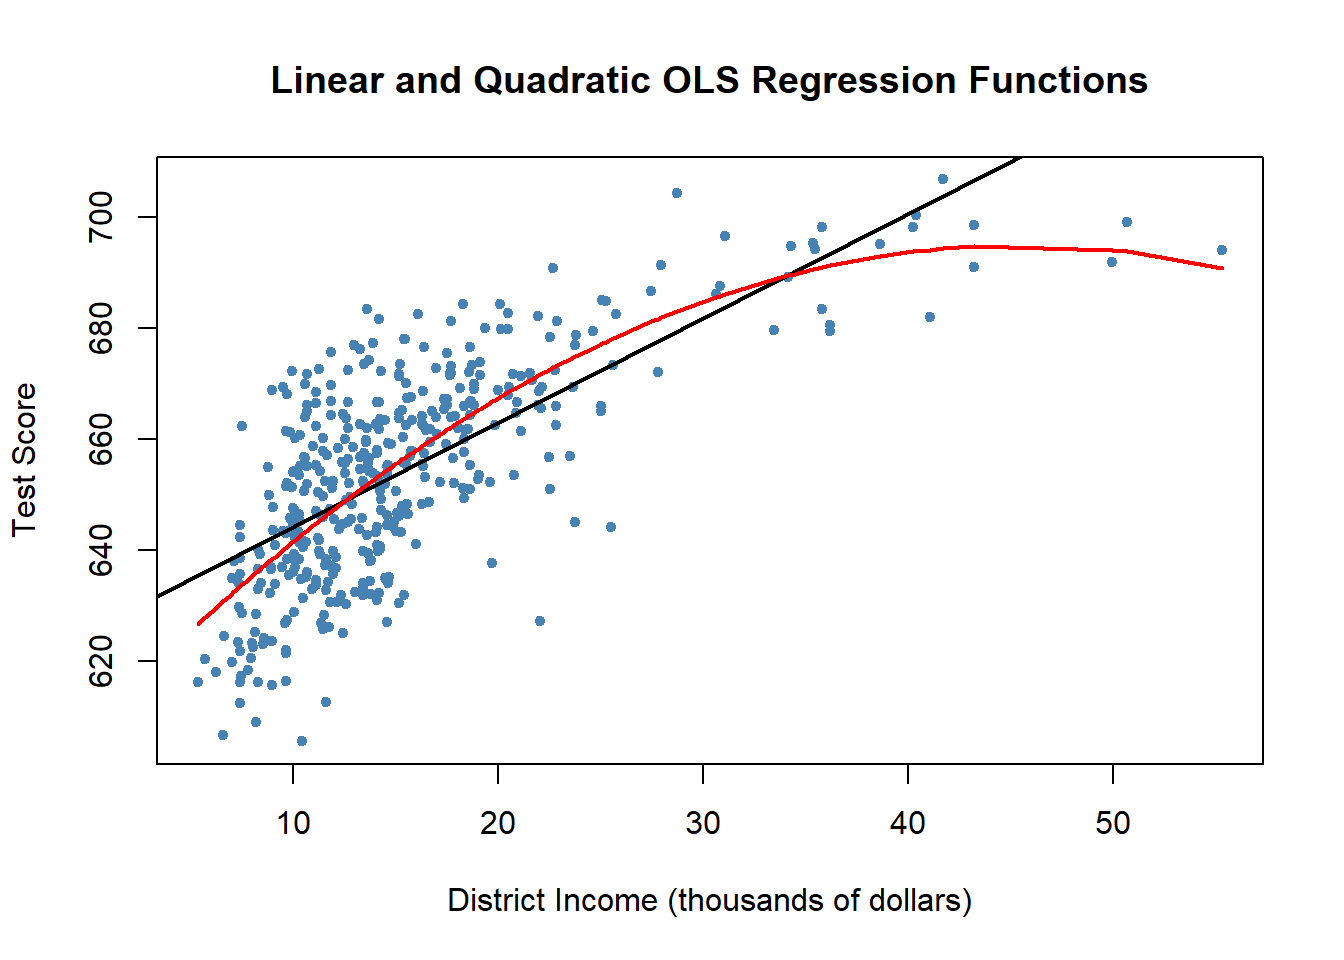
\includegraphics{ITER_files/figure-latex/unnamed-chunk-165-1} \end{center}

\hypertarget{tsdotoe}{\section{The Sampling Distribution of the OLS
Estimator}\label{tsdotoe}}

Because \(\hat{\beta}_0\) and \(\hat{\beta}_1\) are computed from a
sample, the estimators themselves are random variables with a
probability distribution --- the so-called sampling distribution of the
estimators --- which describes the values they could take on over
different samples. Although the sampling distribution of \(\hat\beta_0\)
and \(\hat\beta_1\) can be complicated when the sample size is small and
generally changes with the number of observations, \(n\), it is
possible, provided the assumptions discussed in the book are valid, to
make certain statements about it that hold for all \(n\). In particular
\[ E(\hat{\beta}_0) = \beta_0 \ \ \text{and} \ \  E(\hat{\beta}_1) = \beta_1,\]
that is, \(\hat\beta_0\) and \(\hat\beta_1\) are unbiased estimators of
\(\beta_0\) and \(\beta_1\), the true parameters. If the sample is
sufficiently large, by the central limit theorem the \emph{joint}
sampling distribution of the estimators is well approximated by the
bivariate normal distribution (2.1). This implies that the marginal
distributions are also normal in large samples. Core facts on the
large-sample distributions of \(\hat\beta_0\) and \(\hat\beta_1\) are
presented in Key Concept 4.4.

\begin{keyconcepts}[Large Sample Distribution of $\hat\beta_0$ and $\hat\beta_1$]{4.4}
If the least squares assumptions in Key Concept 4.3 hold, then in large samples $\hat\beta_0$ and $\hat\beta_1$ have a joint normal sampling distribution. The large sample normal distribution of $\hat\beta_1$ is $\mathcal{N}(\beta_1, \sigma^2_{\hat\beta_1})$, where the variance of the distribution, $\sigma^2_{\hat\beta_1}$, is 

\begin{equation}
\sigma^2_{\hat\beta_1} = \frac{1}{n} \frac{Var \left[ \left(X_i - \mu_X \right) u_i  \right]}  {\left[  Var \left(X_i \right)  \right]^2}.
\end{equation}

The large sample normal distribution of $\hat\beta_0$ is $\mathcal{N}(\beta_0, \sigma^2_{\hat\beta_0})$ with

\begin{equation}
\sigma^2_{\hat\beta_0} =  \frac{1}{n} \frac{Var \left( H_i u_i \right)}{ \left[  E \left(H_i^2  \right)  \right]^2 } \ , \ \text{where} \ \ H_i = 1 - \left[ \frac{\mu_X} {E \left( X_i^2\right)} \right] X_i.
\end{equation}

The interactive simulation below continuously generates random samples $(X_i,Y_i)$ of $200$ observations where $E(Y\vert X) = 100 + 3X$, estimates a simple regression model, stores the estimate of the slope $\beta_1$ and visualizes the distribution of the $\widehat{\beta}_1$s observed so far using a histogram. The idea here is that for a large number of $\widehat{\beta}_1$s, the histogram gives a good approximation of the sampling distribution of the estimator. By decreasing the time between two sampling iterations, it becomes clear that the shape of the histogram approaches the characteristic bell shape of a normal distribution centered at the true slope of $3$.\vspace{0.5cm}

\begin{center}\textit{This interactive part of the book is only available in the HTML version.}\end{center}

\end{keyconcepts}

\subsection*{Simulation Study 1}\label{simulation-study-1}
\addcontentsline{toc}{subsection}{Simulation Study 1}

Whether the statements of Key Concept 4.4 really hold can also be
verified using \texttt{R}. For this we first we build our own population
of \(100000\) observations in total. To do this we need values for the
independent variable \(X\), for the error term \(u\), and for the
parameters \(\beta_0\) and \(\beta_1\). With these combined in a simple
regression model, we compute the dependent variable \(Y\). In our
example we generate the numbers \(X_i\), \(i = 1\), \ldots{} ,\(100000\)
by drawing a random sample from a uniform distribution on the interval
\([0,20]\). The realizations of the error terms \(u_i\) are drawn from a
standard normal distribution with parameters \(\mu = 0\) and
\(\sigma^2 = 100\) (note that \texttt{rnorm()} requires \(\sigma\) as
input for the argument \texttt{sd}, see \texttt{?rnorm}). Furthermore we
chose \(\beta_0 = -2\) and \(\beta_1 = 3.5\) so the true model is

\[ Y_i = -2 + 3.5 \cdot X_i. \]

Finally, we store the results in a data.frame.

\begin{Shaded}
\begin{Highlighting}[]
\CommentTok{# simulate data}
\NormalTok{N <-}\StringTok{ }\DecValTok{100000}
\NormalTok{X <-}\StringTok{ }\KeywordTok{runif}\NormalTok{(N, }\DataTypeTok{min =} \DecValTok{0}\NormalTok{, }\DataTypeTok{max =} \DecValTok{20}\NormalTok{)}
\NormalTok{u <-}\StringTok{ }\KeywordTok{rnorm}\NormalTok{(N, }\DataTypeTok{sd =} \DecValTok{10}\NormalTok{)}

\CommentTok{# population regression}
\NormalTok{Y <-}\StringTok{ }\OperatorTok{-}\DecValTok{2} \OperatorTok{+}\StringTok{ }\FloatTok{3.5} \OperatorTok{*}\StringTok{ }\NormalTok{X }\OperatorTok{+}\StringTok{ }\NormalTok{u}
\NormalTok{population <-}\StringTok{ }\KeywordTok{data.frame}\NormalTok{(X, Y)}
\end{Highlighting}
\end{Shaded}

From now on we will consider the previously generated data as the true
population (which of course would be \emph{unknown} in a real world
application, otherwise there would be no reason to draw a random sample
in the first place). The knowledge about the true population and the
true relationship between \(Y\) and \(X\) can be used to verify the
statements made in Key Concept 4.4.

First, let us calculate the true variances \(\sigma^2_{\hat{\beta}_0}\)
and \(\sigma^2_{\hat{\beta}_1}\) for a randomly drawn sample of size
\(n = 100\).

\begin{Shaded}
\begin{Highlighting}[]
\CommentTok{# set sample size}
\NormalTok{n <-}\StringTok{ }\DecValTok{100}

\CommentTok{# compute the variance of beta_hat_0}
\NormalTok{H_i <-}\StringTok{ }\DecValTok{1} \OperatorTok{-}\StringTok{ }\KeywordTok{mean}\NormalTok{(X) }\OperatorTok{/}\StringTok{ }\KeywordTok{mean}\NormalTok{(X}\OperatorTok{^}\DecValTok{2}\NormalTok{) }\OperatorTok{*}\StringTok{ }\NormalTok{X}
\NormalTok{var_b0 <-}\StringTok{ }\KeywordTok{var}\NormalTok{(H_i }\OperatorTok{*}\StringTok{ }\NormalTok{u) }\OperatorTok{/}\StringTok{ }\NormalTok{(n }\OperatorTok{*}\StringTok{ }\KeywordTok{mean}\NormalTok{(H_i}\OperatorTok{^}\DecValTok{2}\NormalTok{)}\OperatorTok{^}\DecValTok{2}\NormalTok{ )}

\CommentTok{# compute the variance of hat_beta_1}
\NormalTok{var_b1 <-}\StringTok{ }\KeywordTok{var}\NormalTok{( ( X }\OperatorTok{-}\StringTok{ }\KeywordTok{mean}\NormalTok{(X) ) }\OperatorTok{*}\StringTok{ }\NormalTok{u ) }\OperatorTok{/}\StringTok{ }\NormalTok{(}\DecValTok{100} \OperatorTok{*}\StringTok{ }\KeywordTok{var}\NormalTok{(X)}\OperatorTok{^}\DecValTok{2}\NormalTok{)}
\end{Highlighting}
\end{Shaded}

\begin{Shaded}
\begin{Highlighting}[]
\CommentTok{# print variances to the console}
\NormalTok{var_b0}
\end{Highlighting}
\end{Shaded}

\begin{verbatim}
## [1] 4.045066
\end{verbatim}

\begin{Shaded}
\begin{Highlighting}[]
\NormalTok{var_b1}
\end{Highlighting}
\end{Shaded}

\begin{verbatim}
## [1] 0.03018694
\end{verbatim}

Now let us assume that we do not know the true values of \(\beta_0\) and
\(\beta_1\) and that it is not possible to observe the whole population.
However, we can observe a random sample of \(n\) observations. Then, it
would not be possible to compute the true parameters but we could obtain
estimates of \(\beta_0\) and \(\beta_1\) from the sample data using OLS.
However, we know that these estimates are outcomes of random variables
themselves since the observations are randomly sampled from the
population. Key Concept 4.4 describes their distributions for large
\(n\). When drawing a single sample of size \(n\) it is not possible to
make any statement about these distributions. Things change if we repeat
the sampling scheme many times and compute the estimates for each
sample: using this procedure we simulate outcomes of the respective
distributions.

To achieve this in R, we employ the following approach:

\begin{itemize}
\tightlist
\item
  We assign the number of repetitions, say \(10000\), to \texttt{reps}
  and then initialize a matrix \texttt{fit} were the estimates obtained
  in each sampling iteration shall be stored row-wise. Thus \texttt{fit}
  has to be a matrix of dimensions \texttt{reps}\(\times2\).
\item
  In the next step we draw \texttt{reps} random samples of size
  \texttt{n} from the population and obtain the OLS estimates for each
  sample. The results are stored as row entries in the outcome matrix
  \texttt{fit}. This is done using a \texttt{for()} loop.
\item
  At last, we estimate variances of both estimators using the sampled
  outcomes and plot histograms of the latter. We also add a plot of the
  density functions belonging to the distributions that follow from Key
  Concept 4.4. The function \texttt{bquote()} is used to obtain math
  expressions in the titles and labels of both plots. See
  \texttt{?bquote}.
\end{itemize}

\begin{Shaded}
\begin{Highlighting}[]
\CommentTok{# set repetitions and sample size}
\NormalTok{n <-}\StringTok{ }\DecValTok{100}
\NormalTok{reps <-}\StringTok{ }\DecValTok{10000}

\CommentTok{# initialize the matrix of outcomes}
\NormalTok{fit <-}\StringTok{ }\KeywordTok{matrix}\NormalTok{(}\DataTypeTok{ncol =} \DecValTok{2}\NormalTok{, }\DataTypeTok{nrow =}\NormalTok{ reps)}

\CommentTok{# loop sampling and estimation of the coefficients}
\ControlFlowTok{for}\NormalTok{ (i }\ControlFlowTok{in} \DecValTok{1}\OperatorTok{:}\NormalTok{reps)\{}
  
\NormalTok{ sample <-}\StringTok{ }\NormalTok{population[}\KeywordTok{sample}\NormalTok{(}\DecValTok{1}\OperatorTok{:}\NormalTok{N, n), ]}
\NormalTok{ fit[i, ] <-}\StringTok{ }\KeywordTok{lm}\NormalTok{(Y }\OperatorTok{~}\StringTok{ }\NormalTok{X, }\DataTypeTok{data =}\NormalTok{ sample)}\OperatorTok{$}\NormalTok{coefficients}
 
\NormalTok{\}}

\CommentTok{# compute variance estimates using outcomes}
\KeywordTok{var}\NormalTok{(fit[, }\DecValTok{1}\NormalTok{])}
\end{Highlighting}
\end{Shaded}

\begin{verbatim}
## [1] 4.057089
\end{verbatim}

\begin{Shaded}
\begin{Highlighting}[]
\KeywordTok{var}\NormalTok{(fit[, }\DecValTok{2}\NormalTok{])}
\end{Highlighting}
\end{Shaded}

\begin{verbatim}
## [1] 0.03021784
\end{verbatim}

\begin{Shaded}
\begin{Highlighting}[]
\CommentTok{# divide plotting area as 1-by-2 array}
\KeywordTok{par}\NormalTok{(}\DataTypeTok{mfrow =} \KeywordTok{c}\NormalTok{(}\DecValTok{1}\NormalTok{, }\DecValTok{2}\NormalTok{))}

\CommentTok{# plot histograms of beta_0 estimates}
\KeywordTok{hist}\NormalTok{(fit[, }\DecValTok{1}\NormalTok{],}
     \DataTypeTok{cex.main =} \DecValTok{1}\NormalTok{,}
     \DataTypeTok{main =} \KeywordTok{bquote}\NormalTok{(The }\OperatorTok{~}\StringTok{ }\NormalTok{Distribution  }\OperatorTok{~}\StringTok{ }\NormalTok{of }\OperatorTok{~}\StringTok{ }\DecValTok{10000} \OperatorTok{~}\StringTok{ }\NormalTok{beta[}\DecValTok{0}\NormalTok{] }\OperatorTok{~}\StringTok{ }\NormalTok{Estimates), }
     \DataTypeTok{xlab =} \KeywordTok{bquote}\NormalTok{(}\KeywordTok{hat}\NormalTok{(beta)[}\DecValTok{0}\NormalTok{]), }
     \DataTypeTok{freq =}\NormalTok{ F)}

\CommentTok{# add true distribution to plot}
\KeywordTok{curve}\NormalTok{(}\KeywordTok{dnorm}\NormalTok{(x, }
            \OperatorTok{-}\DecValTok{2}\NormalTok{, }
            \KeywordTok{sqrt}\NormalTok{(var_b0)), }
      \DataTypeTok{add =}\NormalTok{ T, }
      \DataTypeTok{col =} \StringTok{"darkred"}\NormalTok{)}

\CommentTok{# plot histograms of beta_hat_1 }
\KeywordTok{hist}\NormalTok{(fit[, }\DecValTok{2}\NormalTok{],}
    \DataTypeTok{cex.main =} \DecValTok{1}\NormalTok{,}
     \DataTypeTok{main =} \KeywordTok{bquote}\NormalTok{(The }\OperatorTok{~}\StringTok{ }\NormalTok{Distribution  }\OperatorTok{~}\StringTok{ }\NormalTok{of }\OperatorTok{~}\StringTok{ }\DecValTok{10000} \OperatorTok{~}\StringTok{ }\NormalTok{beta[}\DecValTok{1}\NormalTok{] }\OperatorTok{~}\StringTok{ }\NormalTok{Estimates), }
     \DataTypeTok{xlab =} \KeywordTok{bquote}\NormalTok{(}\KeywordTok{hat}\NormalTok{(beta)[}\DecValTok{1}\NormalTok{]), }
     \DataTypeTok{freq =}\NormalTok{ F)}

\CommentTok{# add true distribution to plot}
\KeywordTok{curve}\NormalTok{(}\KeywordTok{dnorm}\NormalTok{(x, }
            \FloatTok{3.5}\NormalTok{, }
            \KeywordTok{sqrt}\NormalTok{(var_b1)), }
      \DataTypeTok{add =}\NormalTok{ T, }
      \DataTypeTok{col =} \StringTok{"darkred"}\NormalTok{)}
\end{Highlighting}
\end{Shaded}

\begin{center}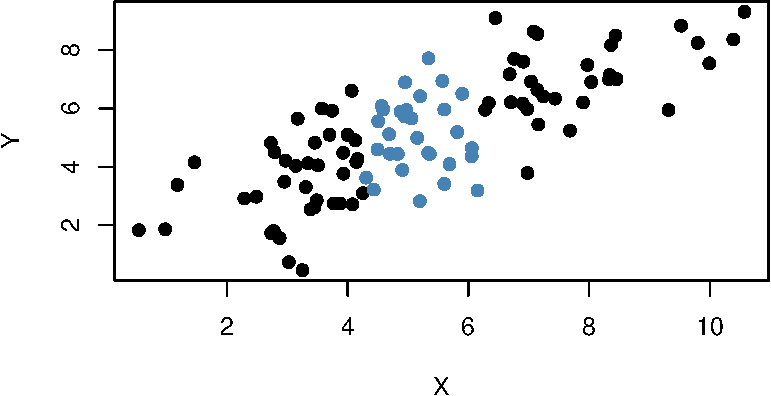
\includegraphics{ITER_files/figure-latex/unnamed-chunk-172-1} \end{center}

Our variance estimates support the statements made in Key Concept 4.4,
coming close to the theoretical values. The histograms suggest that the
distributions of the estimators can be well approximated by the
respective theoretical normal distributions stated in Key Concept 4.4.

\subsection*{Simulation Study 2}\label{simulation-study-2}
\addcontentsline{toc}{subsection}{Simulation Study 2}

A further result implied by Key Concept 4.4 is that both estimators are
consistent, i.e., they converge in probability to the true parameters we
are interested in. This is because they are asymptotically unbiased and
their variances converge to \(0\) as \(n\) increases. We can check this
by repeating the simulation above for a sequence of increasing sample
sizes. This means we no longer assign the sample size but a
\emph{vector} of sample sizes: \texttt{n <- c(...)}. Let us look at the
distributions of \(\beta_1\). The idea here is to add an additional call
of \texttt{for()} to the code. This is done in order to loop over the
vector of sample sizes \texttt{n}. For each of the sample sizes we carry
out the same simulation as before but plot a density estimate for the
outcomes of each iteration over \texttt{n}. Notice that we have to
change \texttt{n} to \texttt{n[j]} in the inner loop to ensure that the
\texttt{j}\(^{th}\) element of \texttt{n} is used. In the simulation, we
use sample sizes of \(100, 250, 1000\) and \(3000\). Consequently we
have a total of four distinct simulations using different sample sizes.

\begin{Shaded}
\begin{Highlighting}[]
\CommentTok{# set seed for reproducibility}
\KeywordTok{set.seed}\NormalTok{(}\DecValTok{1}\NormalTok{)}

\CommentTok{# set repetitions and the vector of sample sizes}
\NormalTok{reps <-}\StringTok{ }\DecValTok{1000}
\NormalTok{n <-}\StringTok{ }\KeywordTok{c}\NormalTok{(}\DecValTok{100}\NormalTok{, }\DecValTok{250}\NormalTok{, }\DecValTok{1000}\NormalTok{, }\DecValTok{3000}\NormalTok{)}

\CommentTok{# initialize the matrix of outcomes}
\NormalTok{fit <-}\StringTok{ }\KeywordTok{matrix}\NormalTok{(}\DataTypeTok{ncol =} \DecValTok{2}\NormalTok{, }\DataTypeTok{nrow =}\NormalTok{ reps)}

\CommentTok{# divide the plot panel in a 2-by-2 array}
\KeywordTok{par}\NormalTok{(}\DataTypeTok{mfrow =} \KeywordTok{c}\NormalTok{(}\DecValTok{2}\NormalTok{, }\DecValTok{2}\NormalTok{))}

\CommentTok{# loop sampling and plotting}

\CommentTok{# outer loop over n}
\ControlFlowTok{for}\NormalTok{ (j }\ControlFlowTok{in} \DecValTok{1}\OperatorTok{:}\KeywordTok{length}\NormalTok{(n)) \{}
  
  \CommentTok{# inner loop: sampling and estimating of the coefficients}
  \ControlFlowTok{for}\NormalTok{ (i }\ControlFlowTok{in} \DecValTok{1}\OperatorTok{:}\NormalTok{reps)\{}
    
\NormalTok{    sample <-}\StringTok{ }\NormalTok{population[}\KeywordTok{sample}\NormalTok{(}\DecValTok{1}\OperatorTok{:}\NormalTok{N, n[j]), ]}
\NormalTok{    fit[i, ] <-}\StringTok{ }\KeywordTok{lm}\NormalTok{(Y }\OperatorTok{~}\StringTok{ }\NormalTok{X, }\DataTypeTok{data =}\NormalTok{ sample)}\OperatorTok{$}\NormalTok{coefficients}
    
\NormalTok{  \}}
  
  \CommentTok{# draw density estimates}
  \KeywordTok{plot}\NormalTok{(}\KeywordTok{density}\NormalTok{(fit[ ,}\DecValTok{2}\NormalTok{]), }\DataTypeTok{xlim=}\KeywordTok{c}\NormalTok{(}\FloatTok{2.5}\NormalTok{, }\FloatTok{4.5}\NormalTok{), }
       \DataTypeTok{col =}\NormalTok{ j, }
       \DataTypeTok{main =} \KeywordTok{paste}\NormalTok{(}\StringTok{"n="}\NormalTok{, n[j]), }
       \DataTypeTok{xlab =} \KeywordTok{bquote}\NormalTok{(}\KeywordTok{hat}\NormalTok{(beta)[}\DecValTok{1}\NormalTok{]))}
  
\NormalTok{\}}
\end{Highlighting}
\end{Shaded}

\begin{center}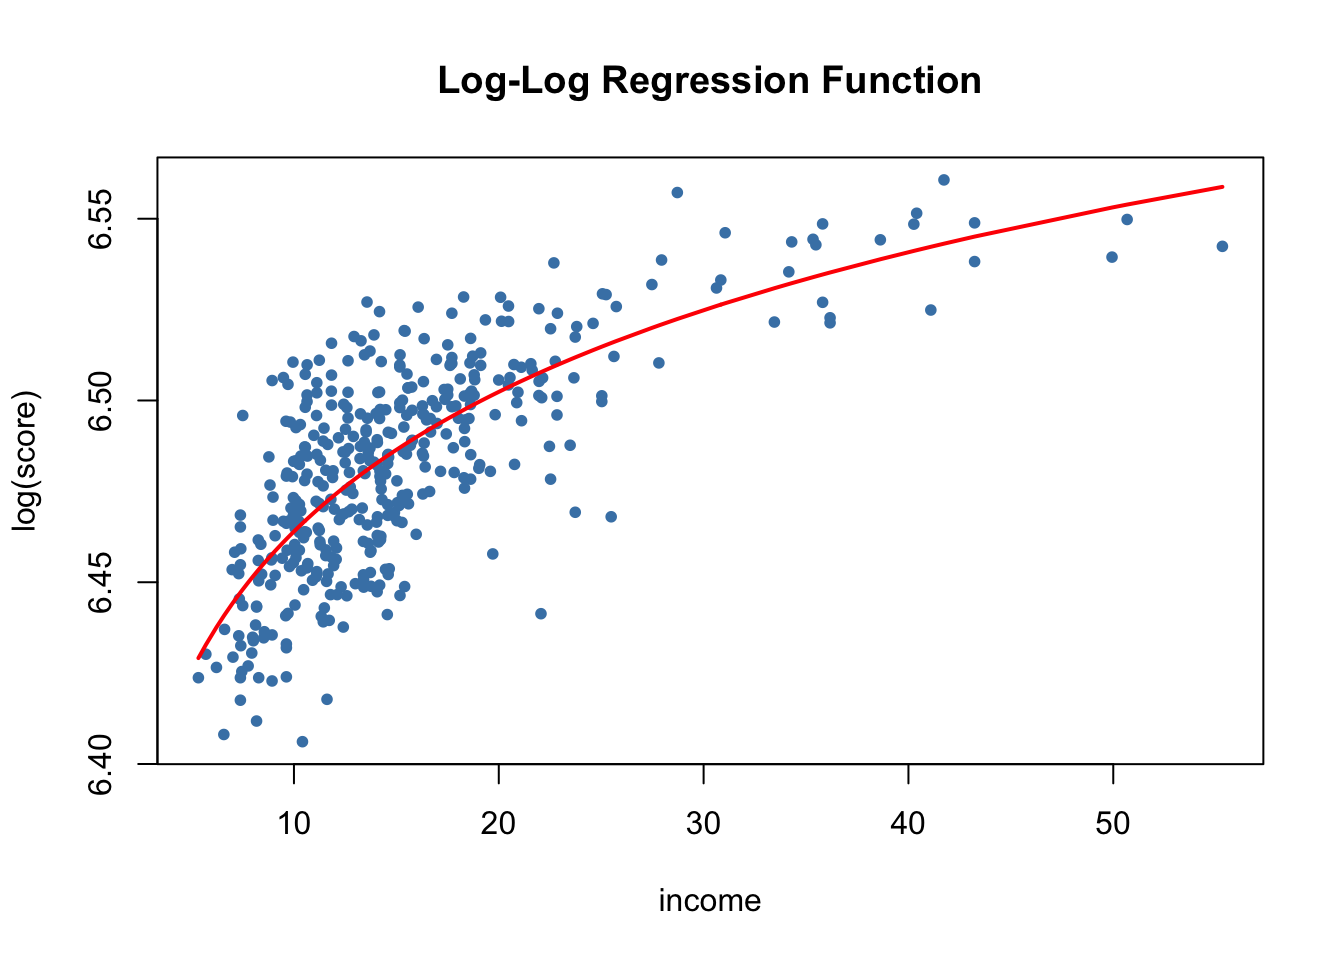
\includegraphics{ITER_files/figure-latex/unnamed-chunk-173-1} \end{center}

We find that, as \(n\) increases, the distribution of \(\hat\beta_1\)
concentrates around its mean, i.e., its variance decreases. Put
differently, the likelihood of observing estimates close to the true
value of \(\beta_1 = 3.5\) grows as we increase the sample size. The
same behavior can be observed if we analyze the distribution of
\(\hat\beta_0\) instead.

\subsection*{Simulation Study 3}\label{simulation-study-3}
\addcontentsline{toc}{subsection}{Simulation Study 3}

Furthermore, (4.1) reveals that the variance of the OLS estimator for
\(\beta_1\) decreases as the variance of the \(X_i\) increases. In other
words, as we increase the amount of information provided by the
regressor, that is, increasing \(Var(X)\), which is used to estimate
\(\beta_1\), we become more confident that the estimate is close to the
true value (i.e., \(Var(\hat\beta_1)\) decreases). We can visualize this
by reproducing Figure 4.6 from the book. To do this, we sample
observations \((X_i,Y_i)\), \(i=1,\dots,100\) from a bivariate normal
distribution with

\[E(X)=E(Y)=5,\] \[Var(X)=Var(Y)=5\] and \[Cov(X,Y)=4.\]

Formally, this is written down as

\begin{align}
  \begin{pmatrix}
    X \\
    Y \\
  \end{pmatrix}
  \overset{i.i.d.}{\sim} & \ \mathcal{N} 
  \left[
    \begin{pmatrix}
      5 \\
      5 \\
    \end{pmatrix}, \ 
    \begin{pmatrix}
      5 & 4 \\
      4 & 5 \\
    \end{pmatrix}
  \right]. \tag{4.3}
\end{align}

To carry out the random sampling, we make use of the function
\texttt{mvrnorm()} from the package \texttt{MASS} \citep{R-MASS} which
allows to draw random samples from multivariate normal distributions,
see \texttt{?mvtnorm}. Next, we use \texttt{subset()} to split the
sample into two subsets such that the first set, \texttt{set1}, consists
of observations that fulfill the condition
\(\lvert X - \overline{X} \rvert > 1\) and the second set,
\texttt{set2}, includes the remainder of the sample. We then plot both
sets and use different colors to distinguish the observations.

\begin{Shaded}
\begin{Highlighting}[]
\CommentTok{# load the MASS package}
\KeywordTok{library}\NormalTok{(MASS)}

\CommentTok{# set seed for reproducibility}
\KeywordTok{set.seed}\NormalTok{(}\DecValTok{4}\NormalTok{)}

\CommentTok{# simulate bivarite normal data}
\NormalTok{bvndata <-}\StringTok{ }\KeywordTok{mvrnorm}\NormalTok{(}\DecValTok{100}\NormalTok{, }
                \DataTypeTok{mu =} \KeywordTok{c}\NormalTok{(}\DecValTok{5}\NormalTok{, }\DecValTok{5}\NormalTok{), }
                \DataTypeTok{Sigma =} \KeywordTok{cbind}\NormalTok{(}\KeywordTok{c}\NormalTok{(}\DecValTok{5}\NormalTok{, }\DecValTok{4}\NormalTok{), }\KeywordTok{c}\NormalTok{(}\DecValTok{4}\NormalTok{, }\DecValTok{5}\NormalTok{))) }

\CommentTok{# assign column names / convert to data.frame}
\KeywordTok{colnames}\NormalTok{(bvndata) <-}\StringTok{ }\KeywordTok{c}\NormalTok{(}\StringTok{"X"}\NormalTok{, }\StringTok{"Y"}\NormalTok{)}
\NormalTok{bvndata <-}\StringTok{ }\KeywordTok{as.data.frame}\NormalTok{(bvndata)}

\CommentTok{# subset the data}
\NormalTok{set1 <-}\StringTok{ }\KeywordTok{subset}\NormalTok{(bvndata, }\KeywordTok{abs}\NormalTok{(}\KeywordTok{mean}\NormalTok{(X) }\OperatorTok{-}\StringTok{ }\NormalTok{X) }\OperatorTok{>}\StringTok{ }\DecValTok{1}\NormalTok{)}
\NormalTok{set2 <-}\StringTok{ }\KeywordTok{subset}\NormalTok{(bvndata, }\KeywordTok{abs}\NormalTok{(}\KeywordTok{mean}\NormalTok{(X) }\OperatorTok{-}\StringTok{ }\NormalTok{X) }\OperatorTok{<=}\StringTok{ }\DecValTok{1}\NormalTok{)}

\CommentTok{# plot both data sets}
\KeywordTok{plot}\NormalTok{(set1, }
     \DataTypeTok{xlab =} \StringTok{"X"}\NormalTok{, }
     \DataTypeTok{ylab =} \StringTok{"Y"}\NormalTok{, }
     \DataTypeTok{pch =} \DecValTok{19}\NormalTok{)}

\KeywordTok{points}\NormalTok{(set2, }
       \DataTypeTok{col =} \StringTok{"steelblue"}\NormalTok{, }
       \DataTypeTok{pch =} \DecValTok{19}\NormalTok{)}
\end{Highlighting}
\end{Shaded}

\begin{center}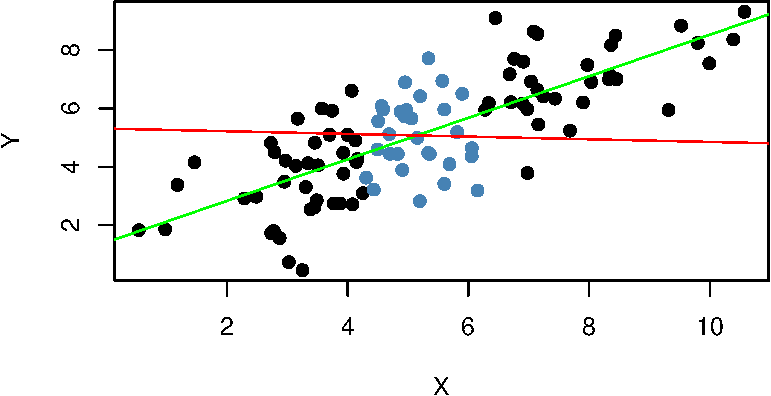
\includegraphics{ITER_files/figure-latex/unnamed-chunk-174-1} \end{center}

It is clear that observations that are close to the sample average of
the \(X_i\) have less variance than those that are farther away. Now, if
we were to draw a line as accurately as possible through either of the
two sets it is intuitive that choosing the observations indicated by the
black dots, i.e., using the set of observations which has larger
variance than the blue ones, would result in a more precise line. Now,
let us use OLS to estimate slope and intercept for both sets of
observations. We then plot the observations along with both regression
lines.

\begin{Shaded}
\begin{Highlighting}[]
\CommentTok{# estimate both regression lines}
\NormalTok{lm.set1 <-}\StringTok{ }\KeywordTok{lm}\NormalTok{(Y }\OperatorTok{~}\StringTok{ }\NormalTok{X, }\DataTypeTok{data =}\NormalTok{ set1)}
\NormalTok{lm.set2 <-}\StringTok{ }\KeywordTok{lm}\NormalTok{(Y }\OperatorTok{~}\StringTok{ }\NormalTok{X, }\DataTypeTok{data =}\NormalTok{ set2)}

\CommentTok{# plot observations}
\KeywordTok{plot}\NormalTok{(set1, }\DataTypeTok{xlab =} \StringTok{"X"}\NormalTok{, }\DataTypeTok{ylab =} \StringTok{"Y"}\NormalTok{, }\DataTypeTok{pch =} \DecValTok{19}\NormalTok{)}
\KeywordTok{points}\NormalTok{(set2, }\DataTypeTok{col =} \StringTok{"steelblue"}\NormalTok{, }\DataTypeTok{pch =} \DecValTok{19}\NormalTok{)}

\CommentTok{# add both lines to the plot}
\KeywordTok{abline}\NormalTok{(lm.set1, }\DataTypeTok{col =} \StringTok{"green"}\NormalTok{)}
\KeywordTok{abline}\NormalTok{(lm.set2, }\DataTypeTok{col =} \StringTok{"red"}\NormalTok{)}
\end{Highlighting}
\end{Shaded}

\begin{center}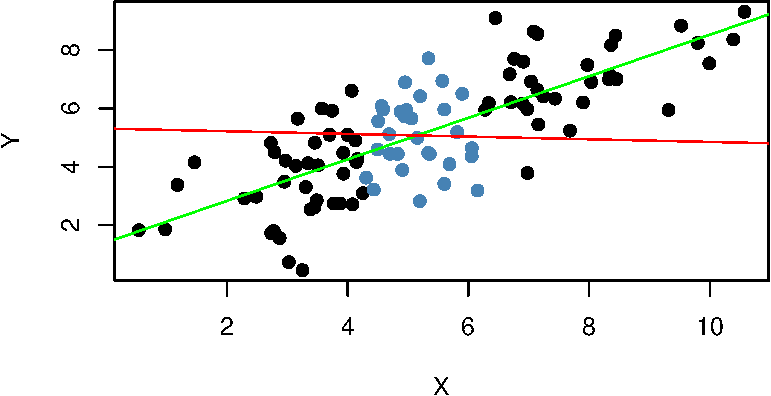
\includegraphics{ITER_files/figure-latex/unnamed-chunk-175-1} \end{center}

Evidently, the green regression line does far better in describing data
sampled from the bivariate normal distribution stated in (4.3) than the
red line. This is a nice example for demonstrating why we are interested
in a high variance of the regressor \(X\): more variance in the \(X_i\)
means more information from which the precision of the estimation
benefits.

\section{Exercises}\label{exercises-2}

\begin{center}\textit{This interactive part of the book is only available in the HTML version.}\end{center}

\chapter{Hypothesis Tests and Confidence Intervals in the Simple Linear
Regression Model}\label{htaciitslrm}

This chapter, continues our treatment of the simple linear regression
model. The following subsections discuss how we may use our knowledge
about the sampling distribution of the OLS estimator in order to make
statements regarding its uncertainty.

These subsections cover the following topics:

\begin{itemize}
\item
  Testing Hypotheses regarding regression coefficients.
\item
  Confidence intervals for regression coefficients.
\item
  Regression when \(X\) is a dummy variable.
\item
  Heteroskedasticity and Homoskedasticity.
\end{itemize}

The packages \texttt{AER} \citep{R-AER} and \texttt{scales}
\citep{R-scales} are required for reproduction of the code chunks
presented throughout this chapter. The package \texttt{scales} provides
additional generic plot scaling methods. Make sure both packages are
installed before you proceed. The safest way to do so is by checking
whether the following code chunk executes without any errors.

\begin{Shaded}
\begin{Highlighting}[]
\KeywordTok{library}\NormalTok{(AER)}
\KeywordTok{library}\NormalTok{(scales)}
\end{Highlighting}
\end{Shaded}

\section{Testing Two-Sided Hypotheses Concerning the Slope
Coefficient}\label{testing-two-sided-hypotheses-concerning-the-slope-coefficient}

Using the fact that \(\hat{\beta}_1\) is approximately normally
distributed in large samples (see \protect\hyperlink{tsdotoe}{Key
Concept 4.4}), testing hypotheses about the true value \(\beta_1\) can
be done as in Chapter \ref{potsm}.

\begin{keyconcepts}[General Form of the $t$-Statistic]{5.1}
Remember from Chapter \ref{arosur} that a general $t$-statistic has the form
$$ t = \frac{\text{estimated value} - \text{hypothesized value}}{\text{standard error of the estimator}}.$$
\end{keyconcepts}

\begin{keyconcepts}[Testing Hypotheses regarding $\beta_1$]{5.2}
For testing the hypothesis $H_0: \beta_1 = \beta_{1,0}$, we need to perform the following steps:\newline

\begin{enumerate}
\item Compute the standard error of $\hat{\beta}_1$, $SE(\hat{\beta}_1)$

\[ SE(\hat{\beta}_1) = \sqrt{ \hat{\sigma}^2_{\hat{\beta}_1} } \ \ , \ \ 
  \hat{\sigma}^2_{\hat{\beta}_1} = \frac{1}{n} \times \frac{\frac{1}{n-2} \sum_{i=1}^n (X_i - \overline{X})^2 \hat{u_i}^2 }{ \left[ \frac{1}{n} \sum_{i=1}^n (X_i - \overline{X})^2 \right]^2}.
\]

\item Compute the $t$-statistic

\[ t = \frac{\hat{\beta}_1 - \beta_{1,0}}{ SE(\hat{\beta}_1) }. \]

\item Given a two sided alternative ($H_1:\beta_1 \neq \beta_{1,0}$) we reject at the $5\%$ level if $|t^{act}| > 1.96$ or, equivalently, if the $p$-value is less than $0.05$.\newline  
Recall the definition of the $p$-value:  

  \begin{align*}
    p \text{-value} =& \, \text{Pr}_{H_0} \left[ \left| \frac{ \hat{\beta}_1 - \beta_{1,0} }{ SE(\hat{\beta}_1) } \right| > \left|        \frac{ \hat{\beta}_1^{act} - \beta_{1,0} }{ SE(\hat{\beta}_1) } \right| \right] \\
    =& \, \text{Pr}_{H_0} (|t| > |t^{act}|) \\
    =& \, 2 \cdot \Phi(-|t^{act}|)
  \end{align*}  

The last transformation is due to the normal approximation for large samples.
\end{enumerate}
\end{keyconcepts}

Consider again the OLS regression stored in \texttt{linear\_model} from
Chapter \ref{lrwor} that gave us the regression line

\[ \widehat{TestScore} \ = \underset{(9.47)}{698.9} - \underset{(0.49)}{2.28} \times STR \ , \ R^2=0.051 \ , \ SER=18.6. \]

For testing a hypothesis concerning the slope parameter (the coefficient
on \(STR\)), we need \(SE(\hat{\beta}_1)\), the standard error of the
respective point estimator. As is common in the literature, standard
errors are presented in parentheses below the point estimates.

Key Concept 5.1 reveals that it is rather cumbersome to compute the
standard error and thereby the \(t\)-statistic by hand. The question you
should be asking yourself right now is: can we obtain these values with
minimum effort using \texttt{R}? Yes, we can. Let us first use
\texttt{summary()} to get a summary on the estimated coefficients in
\texttt{linear\_model}.

\textbf{Note}: Throughout the book, robust standard errors are reported.
We consider it instructive keep things simple at the beginning and thus
start out with simple examples that do not allow for robust inference.
Standard errors that are robust to heteroskedasticity are introduced in
Chapter \ref{hah} where we also demonstrate how they can be computed
using \texttt{R}. A discussion of heteroskedasticity-autocorrelation
robust standard errors takes place in Chapter \ref{eodce}.

\begin{Shaded}
\begin{Highlighting}[]
\CommentTok{# print the summary of the coefficients to the console}
\end{Highlighting}
\end{Shaded}

\begin{verbatim}
##               Estimate Std. Error   t value      Pr(>|t|)
## (Intercept) 698.932949  9.4674911 73.824516 6.569846e-242
## STR          -2.279808  0.4798255 -4.751327  2.783308e-06
\end{verbatim}

The second column of the coefficients' summary, reports
\(SE(\hat\beta_0)\) and \(SE(\hat\beta_1)\). Also, in the third column
\texttt{t value}, we find \(t\)-statistics \(t^{act}\) suitable for
tests of the separate hypotheses \(H_0: \beta_0=0\) and
\(H_0: \beta_1=0\). Furthermore, the output provides us with
\(p\)-values corresponding to both tests against the two-sided
alternatives \(H_1:\beta_0\neq0\) respectively \(H_1:\beta_1\neq0\) in
the fourth column of the table.

Let us have a closer look at the test of

\[H_0: \beta_1=0 \ \ \ vs. \ \ \ H_1: \beta_1 \neq 0.\]

We have \[ t^{act} = \frac{-2.279808 - 0}{0.4798255} \approx - 4.75. \]

What does this tell us about the significance of the estimated
coefficient? We reject the null hypothesis at the \(5\%\) level of
significance since \(|t^{act}| > 1.96\). That is, the observed test
statistic falls into the rejection region as
\(p\text{-value} = 2.78\cdot 10^{-6} < 0.05\). We conclude that the
coefficient is significantly different from zero. In other words, we
reject the hypothesis that the class size \emph{has no influence} on the
students test scores at the \(5\%\) level.

Note that although the difference is negligible in the present case as
we will see later, \texttt{summary()} does not perform the normal
approximation but calculates \(p\)-values using the \(t\)-distribution
instead. Generally, the degrees of freedom of the assumed
\(t\)-distribution are determined in the following manner:

\[ \text{DF} = n - k - 1 \]

where \(n\) is the number of observations used to estimate the model and
\(k\) is the number of regressors, excluding the intercept. In our case,
we have \(n=420\) observations and the only regressor is \(STR\) so
\(k=1\). The simplest way to determine the model degrees of freedom is

\begin{Shaded}
\begin{Highlighting}[]
\CommentTok{# determine residual degrees of freedom}
\NormalTok{linear_model}\OperatorTok{$}\NormalTok{df.residual}
\end{Highlighting}
\end{Shaded}

\begin{verbatim}
## [1] 418
\end{verbatim}

Hence, for the assumed sampling distribution of \(\hat\beta_1\) we have

\[\hat\beta_1 \sim t_{418}\] such that the \(p\)-value for a two-sided
significance test can be obtained by executing the following code:

\begin{Shaded}
\begin{Highlighting}[]
\DecValTok{2} \OperatorTok{*}\StringTok{ }\KeywordTok{pt}\NormalTok{(}\OperatorTok{-}\FloatTok{4.751327}\NormalTok{, }\DataTypeTok{df =} \DecValTok{418}\NormalTok{)}
\end{Highlighting}
\end{Shaded}

\begin{verbatim}
## [1] 2.78331e-06
\end{verbatim}

The result is very close to the value provided by \texttt{summary()}.
However since \(n\) is sufficiently large one could just as well use the
standard normal density to compute the \(p\)-value:

\begin{Shaded}
\begin{Highlighting}[]
\DecValTok{2} \OperatorTok{*}\StringTok{ }\KeywordTok{pnorm}\NormalTok{(}\OperatorTok{-}\FloatTok{4.751327}\NormalTok{)}
\end{Highlighting}
\end{Shaded}

\begin{verbatim}
## [1] 2.02086e-06
\end{verbatim}

The difference is indeed negligible. These findings tell us that, if
\(H_0: \beta_1 = 0\) is true and we were to repeat the whole process of
gathering observations and estimating the model, observing a
\(\hat\beta_1 \geq |-2.28|\) is very unlikely!

Using \texttt{R} we may visualize how such a statement is made when
using the normal approximation. This reflects the principles depicted in
figure 5.1 in the book. Do not let the following code chunk deter you:
the code is somewhat longer than the usual examples and looks
unappealing but there is \textbf{a lot} of repetition since color
shadings and annotations are added on both tails of the normal
distribution. We recommend to execute the code step by step in order to
see how the graph is augmented with the annotations.

\begin{Shaded}
\begin{Highlighting}[]
\CommentTok{# Plot the standard normal on the support [-6,6]}
\NormalTok{t <-}\StringTok{ }\KeywordTok{seq}\NormalTok{(}\OperatorTok{-}\DecValTok{6}\NormalTok{, }\DecValTok{6}\NormalTok{, }\FloatTok{0.01}\NormalTok{)}

\KeywordTok{plot}\NormalTok{(}\DataTypeTok{x =}\NormalTok{ t, }
     \DataTypeTok{y =} \KeywordTok{dnorm}\NormalTok{(t, }\DecValTok{0}\NormalTok{, }\DecValTok{1}\NormalTok{), }
     \DataTypeTok{type =} \StringTok{"l"}\NormalTok{, }
     \DataTypeTok{col =} \StringTok{"steelblue"}\NormalTok{, }
     \DataTypeTok{lwd =} \DecValTok{2}\NormalTok{, }
     \DataTypeTok{yaxs =} \StringTok{"i"}\NormalTok{, }
     \DataTypeTok{axes =}\NormalTok{ F, }
     \DataTypeTok{ylab =} \StringTok{""}\NormalTok{, }
     \DataTypeTok{main =} \KeywordTok{expression}\NormalTok{(}\StringTok{"Calculating the p-value of a Two-sided Test when"} \OperatorTok{~}\StringTok{ }\NormalTok{t}\OperatorTok{^}\NormalTok{act }\OperatorTok{~}\StringTok{ "=-0.47"}\NormalTok{), }
     \DataTypeTok{cex.lab =} \FloatTok{0.7}\NormalTok{,}
     \DataTypeTok{cex.main =} \DecValTok{1}\NormalTok{)}

\NormalTok{tact <-}\StringTok{ }\OperatorTok{-}\FloatTok{4.75}

\KeywordTok{axis}\NormalTok{(}\DecValTok{1}\NormalTok{, }\DataTypeTok{at =} \KeywordTok{c}\NormalTok{(}\DecValTok{0}\NormalTok{, }\OperatorTok{-}\FloatTok{1.96}\NormalTok{, }\FloatTok{1.96}\NormalTok{, }\OperatorTok{-}\NormalTok{tact, tact), }\DataTypeTok{cex.axis =} \FloatTok{0.7}\NormalTok{)}

\CommentTok{# Shade the critical regions using polygon():}

\CommentTok{# critical region in left tail}
\KeywordTok{polygon}\NormalTok{(}\DataTypeTok{x =} \KeywordTok{c}\NormalTok{(}\OperatorTok{-}\DecValTok{6}\NormalTok{, }\KeywordTok{seq}\NormalTok{(}\OperatorTok{-}\DecValTok{6}\NormalTok{, }\OperatorTok{-}\FloatTok{1.96}\NormalTok{, }\FloatTok{0.01}\NormalTok{), }\OperatorTok{-}\FloatTok{1.96}\NormalTok{),}
        \DataTypeTok{y =} \KeywordTok{c}\NormalTok{(}\DecValTok{0}\NormalTok{, }\KeywordTok{dnorm}\NormalTok{(}\KeywordTok{seq}\NormalTok{(}\OperatorTok{-}\DecValTok{6}\NormalTok{, }\OperatorTok{-}\FloatTok{1.96}\NormalTok{, }\FloatTok{0.01}\NormalTok{)), }\DecValTok{0}\NormalTok{), }
        \DataTypeTok{col =} \StringTok{'orange'}\NormalTok{)}

\CommentTok{# critical region in right tail}

\KeywordTok{polygon}\NormalTok{(}\DataTypeTok{x =} \KeywordTok{c}\NormalTok{(}\FloatTok{1.96}\NormalTok{, }\KeywordTok{seq}\NormalTok{(}\FloatTok{1.96}\NormalTok{, }\DecValTok{6}\NormalTok{, }\FloatTok{0.01}\NormalTok{), }\DecValTok{6}\NormalTok{),}
        \DataTypeTok{y =} \KeywordTok{c}\NormalTok{(}\DecValTok{0}\NormalTok{, }\KeywordTok{dnorm}\NormalTok{(}\KeywordTok{seq}\NormalTok{(}\FloatTok{1.96}\NormalTok{, }\DecValTok{6}\NormalTok{, }\FloatTok{0.01}\NormalTok{)), }\DecValTok{0}\NormalTok{), }
        \DataTypeTok{col =} \StringTok{'orange'}\NormalTok{)}

\CommentTok{# Add arrows and texts indicating critical regions and the p-value}
\KeywordTok{arrows}\NormalTok{(}\OperatorTok{-}\FloatTok{3.5}\NormalTok{, }\FloatTok{0.2}\NormalTok{, }\OperatorTok{-}\FloatTok{2.5}\NormalTok{, }\FloatTok{0.02}\NormalTok{, }\DataTypeTok{length =} \FloatTok{0.1}\NormalTok{)}
\KeywordTok{arrows}\NormalTok{(}\FloatTok{3.5}\NormalTok{, }\FloatTok{0.2}\NormalTok{, }\FloatTok{2.5}\NormalTok{, }\FloatTok{0.02}\NormalTok{, }\DataTypeTok{length =} \FloatTok{0.1}\NormalTok{)}

\KeywordTok{arrows}\NormalTok{(}\OperatorTok{-}\DecValTok{5}\NormalTok{, }\FloatTok{0.16}\NormalTok{, }\OperatorTok{-}\FloatTok{4.75}\NormalTok{, }\DecValTok{0}\NormalTok{, }\DataTypeTok{length =} \FloatTok{0.1}\NormalTok{)}
\KeywordTok{arrows}\NormalTok{(}\DecValTok{5}\NormalTok{, }\FloatTok{0.16}\NormalTok{, }\FloatTok{4.75}\NormalTok{, }\DecValTok{0}\NormalTok{, }\DataTypeTok{length =} \FloatTok{0.1}\NormalTok{)}

\KeywordTok{text}\NormalTok{(}\OperatorTok{-}\FloatTok{3.5}\NormalTok{, }\FloatTok{0.22}\NormalTok{, }
     \DataTypeTok{labels =} \KeywordTok{expression}\NormalTok{(}\StringTok{"0.025"}\OperatorTok{~}\StringTok{"="}\OperatorTok{~}\KeywordTok{over}\NormalTok{(alpha, }\DecValTok{2}\NormalTok{)),}
     \DataTypeTok{cex =} \FloatTok{0.7}\NormalTok{)}
\KeywordTok{text}\NormalTok{(}\FloatTok{3.5}\NormalTok{, }\FloatTok{0.22}\NormalTok{, }
     \DataTypeTok{labels =} \KeywordTok{expression}\NormalTok{(}\StringTok{"0.025"}\OperatorTok{~}\StringTok{"="}\OperatorTok{~}\KeywordTok{over}\NormalTok{(alpha, }\DecValTok{2}\NormalTok{)),}
     \DataTypeTok{cex =} \FloatTok{0.7}\NormalTok{)}

\KeywordTok{text}\NormalTok{(}\OperatorTok{-}\DecValTok{5}\NormalTok{, }\FloatTok{0.18}\NormalTok{, }
     \DataTypeTok{labels =} \KeywordTok{expression}\NormalTok{(}\KeywordTok{paste}\NormalTok{(}\StringTok{"-|"}\NormalTok{,t[act],}\StringTok{"|"}\NormalTok{)), }
     \DataTypeTok{cex =} \FloatTok{0.7}\NormalTok{)}
\KeywordTok{text}\NormalTok{(}\DecValTok{5}\NormalTok{, }\FloatTok{0.18}\NormalTok{, }
     \DataTypeTok{labels =} \KeywordTok{expression}\NormalTok{(}\KeywordTok{paste}\NormalTok{(}\StringTok{"|"}\NormalTok{,t[act],}\StringTok{"|"}\NormalTok{)), }
     \DataTypeTok{cex =} \FloatTok{0.7}\NormalTok{)}

\CommentTok{# Add ticks indicating critical values at the 0.05-level, t^act and -t^act }
\KeywordTok{rug}\NormalTok{(}\KeywordTok{c}\NormalTok{(}\OperatorTok{-}\FloatTok{1.96}\NormalTok{, }\FloatTok{1.96}\NormalTok{), }\DataTypeTok{ticksize  =} \FloatTok{0.145}\NormalTok{, }\DataTypeTok{lwd =} \DecValTok{2}\NormalTok{, }\DataTypeTok{col =} \StringTok{"darkred"}\NormalTok{)}
\KeywordTok{rug}\NormalTok{(}\KeywordTok{c}\NormalTok{(}\OperatorTok{-}\NormalTok{tact, tact), }\DataTypeTok{ticksize  =} \OperatorTok{-}\FloatTok{0.0451}\NormalTok{, }\DataTypeTok{lwd =} \DecValTok{2}\NormalTok{, }\DataTypeTok{col =} \StringTok{"darkgreen"}\NormalTok{)}
\end{Highlighting}
\end{Shaded}

\begin{center}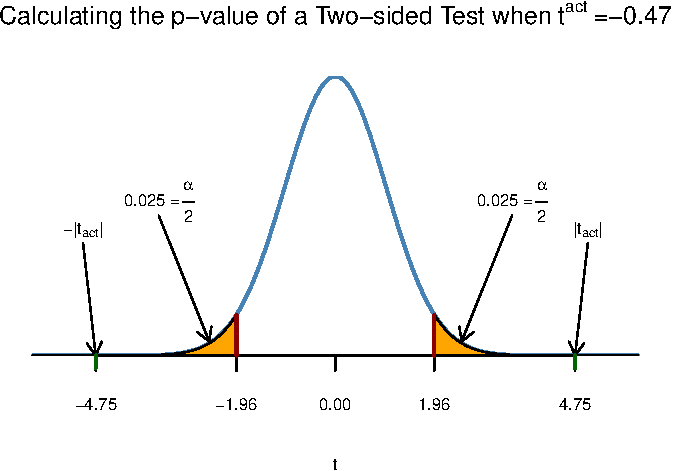
\includegraphics{ITER_files/figure-latex/unnamed-chunk-200-1} \end{center}

The \(p\)-Value is the area under the curve to left of \(-4.75\) plus
the area under the curve to the right of \(4.75\). As we already know
from the calculations above, this value is very small.

\section{Confidence Intervals for Regression Coefficients}\label{cifrc}

As we already know, estimates of the regression coefficients \(\beta_0\)
and \(\beta_1\) are subject to sampling uncertainty, see Chapter
\ref{lrwor}. Therefore, we will \emph{never} exactly estimate the true
value of these parameters from sample data in an empirical application.
However, we may construct confidence intervals for the intercept and the
slope parameter.

A \(95\%\) confidence interval for \(\beta_i\) has two equivalent
definitions:

\begin{itemize}
\tightlist
\item
  The interval is the set of values for which a hypothesis test to the
  level of \(5\%\) cannot be rejected.
\item
  The interval has a probability of \(95\%\) to contain the true value
  of \(\beta_i\). So in \(95\%\) of all samples that could be drawn, the
  confidence interval will cover the true value of \(\beta_i\).
\end{itemize}

We also say that the interval has a confidence level of \(95\%\). The
idea of the confidence interval is summarized in Key Concept 5.3.

\begin{keyconcepts}[A Confidence Interval for $\beta_i$]{5.3}
Imagine you could draw all possible random samples of given size. The interval that contains the true value $\beta_i$ in $95\%$ of all samples is given by the expression

\[ \text{CI}_{0.95}^{\beta_i} = \left[ \hat{\beta}_i - 1.96 \times SE(\hat{\beta}_i) \, , \, \hat{\beta}_i + 1.96 \times SE(\hat{\beta}_i) \right]. \]

Equivalently, this interval can be seen as the set of null hypotheses for which a $5\%$ two-sided hypothesis test does not reject.
\end{keyconcepts}

\subsection*{Simulation Study: Confidence
Intervals}\label{simulation-study-confidence-intervals}
\addcontentsline{toc}{subsection}{Simulation Study: Confidence
Intervals}

To get a better understanding of confidence intervals we conduct another
simulation study. For now, assume that we have the following sample of
\(n=100\) observations on a single variable \(Y\) where

\[ Y_i \overset{i.i.d}{\sim} \mathcal{N}(5,25), \ i = 1, \dots, 100.\]

\begin{Shaded}
\begin{Highlighting}[]
\CommentTok{# set seed for reproducibility}
\KeywordTok{set.seed}\NormalTok{(}\DecValTok{4}\NormalTok{)}

\CommentTok{# generate and plot the sample data}
\NormalTok{Y <-}\StringTok{ }\KeywordTok{rnorm}\NormalTok{(}\DataTypeTok{n =} \DecValTok{100}\NormalTok{, }
           \DataTypeTok{mean =} \DecValTok{5}\NormalTok{, }
           \DataTypeTok{sd =} \DecValTok{5}\NormalTok{)}

\KeywordTok{plot}\NormalTok{(Y, }
     \DataTypeTok{pch =} \DecValTok{19}\NormalTok{, }
     \DataTypeTok{col =} \StringTok{"steelblue"}\NormalTok{)}
\end{Highlighting}
\end{Shaded}

\begin{center}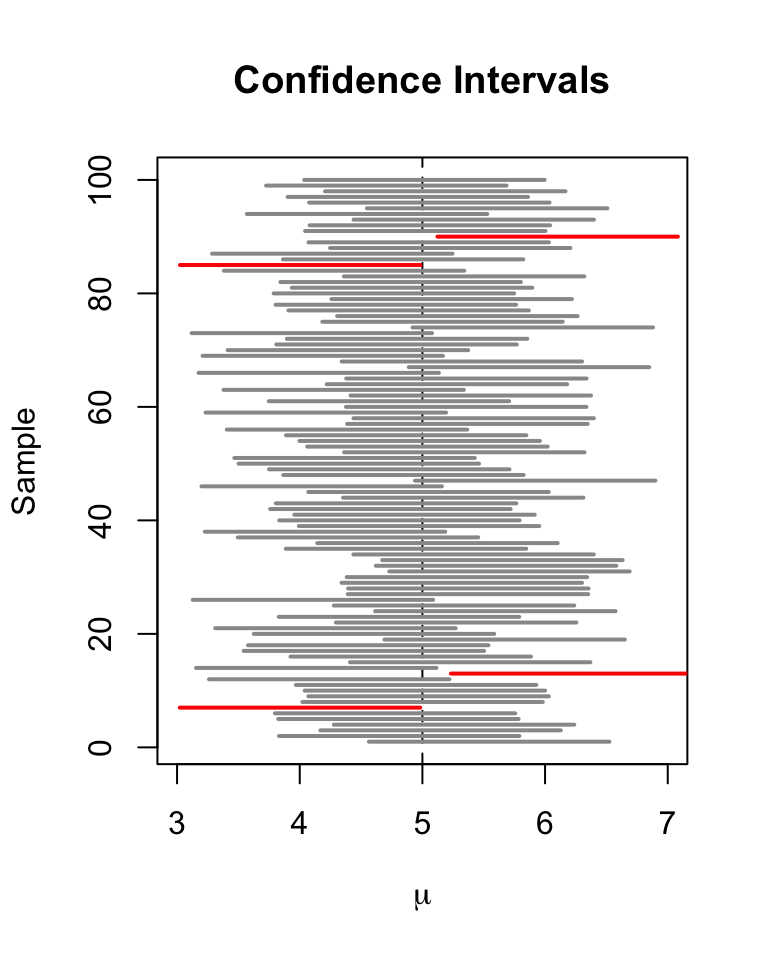
\includegraphics{ITER_files/figure-latex/unnamed-chunk-203-1} \end{center}

We assume that the data is generated by the model

\[ Y_i = \mu + \epsilon_i \]

where \(\mu\) is an unknown constant and we know that
\(\epsilon_i \overset{i.i.d.}{\sim} \mathcal{N}(0,25)\). In this model,
the OLS estimator for \(\mu\) is given by
\[ \hat\mu = \overline{Y} = \frac{1}{n} \sum_{i=1}^n Y_i, \] i.e., the
sample average of the \(Y_i\). It further holds that

\[ SE(\hat\mu) = \frac{\sigma_{\epsilon}}{\sqrt{n}} = \frac{5}{\sqrt{100}} \]

(see Chapter \protect\hyperlink{SVSSDASE}{2}) A large-sample \(95\%\)
confidence interval for \(\mu\) is then given by

\begin{equation} 
CI^{\mu}_{0.95} = \left[\hat\mu - 1.96 \times \frac{5}{\sqrt{100}} \ , \ \hat\mu + 1.96 \times \frac{5}{\sqrt{100}}  \right]. \label{eq:KI}
\end{equation}

It is fairly easy to compute this interval in \texttt{R} by hand. The
following code chunk generates a named vector containing the interval
bounds:

\begin{Shaded}
\begin{Highlighting}[]
\KeywordTok{cbind}\NormalTok{(}\DataTypeTok{CIlower =} \KeywordTok{mean}\NormalTok{(Y) }\OperatorTok{-}\StringTok{ }\FloatTok{1.96} \OperatorTok{*}\StringTok{ }\DecValTok{5} \OperatorTok{/}\StringTok{ }\DecValTok{10}\NormalTok{, }\DataTypeTok{CIupper =} \KeywordTok{mean}\NormalTok{(Y) }\OperatorTok{+}\StringTok{ }\FloatTok{1.96} \OperatorTok{*}\StringTok{ }\DecValTok{5} \OperatorTok{/}\StringTok{ }\DecValTok{10}\NormalTok{)}
\end{Highlighting}
\end{Shaded}

\begin{verbatim}
##       CIlower  CIupper
## [1,] 4.502625 6.462625
\end{verbatim}

Knowing that \(\mu = 5\) we see that, for our example data, the
confidence interval covers true value.

As opposed to real world examples, we can use \texttt{R} to get a better
understanding of confidence intervals by repeatedly sampling data,
estimating \(\mu\) and computing the confidence interval for \(\mu\) as
in \eqref{eq:KI}.

The procedure is as follows:

\begin{itemize}
\tightlist
\item
  We initialize the vectors \texttt{lower} and \texttt{upper} in which
  the simulated interval limits are to be saved. We want to simulate
  \(10000\) intervals so both vectors are set to have this length.
\item
  We use a \texttt{for()} loop to sample \(100\) observations from the
  \(\mathcal{N}(5,25)\) distribution and compute \(\hat\mu\) as well as
  the boundaries of the confidence interval in every iteration of the
  loop.
\item
  At last we join \texttt{lower} and \texttt{upper} in a matrix.
\end{itemize}

\begin{Shaded}
\begin{Highlighting}[]
\CommentTok{# set seed}
\KeywordTok{set.seed}\NormalTok{(}\DecValTok{1}\NormalTok{)}

\CommentTok{# initialize vectors of lower and upper interval boundaries}
\NormalTok{lower <-}\StringTok{ }\KeywordTok{numeric}\NormalTok{(}\DecValTok{10000}\NormalTok{)}
\NormalTok{upper <-}\StringTok{ }\KeywordTok{numeric}\NormalTok{(}\DecValTok{10000}\NormalTok{)}

\CommentTok{# loop sampling / estimation / CI}
\ControlFlowTok{for}\NormalTok{(i }\ControlFlowTok{in} \DecValTok{1}\OperatorTok{:}\DecValTok{10000}\NormalTok{) \{}
  
\NormalTok{  Y <-}\StringTok{ }\KeywordTok{rnorm}\NormalTok{(}\DecValTok{100}\NormalTok{, }\DataTypeTok{mean =} \DecValTok{5}\NormalTok{, }\DataTypeTok{sd =} \DecValTok{5}\NormalTok{)}
\NormalTok{  lower[i] <-}\StringTok{ }\KeywordTok{mean}\NormalTok{(Y) }\OperatorTok{-}\StringTok{ }\FloatTok{1.96} \OperatorTok{*}\StringTok{ }\DecValTok{5} \OperatorTok{/}\StringTok{ }\DecValTok{10}
\NormalTok{  upper[i] <-}\StringTok{ }\KeywordTok{mean}\NormalTok{(Y) }\OperatorTok{+}\StringTok{ }\FloatTok{1.96} \OperatorTok{*}\StringTok{ }\DecValTok{5} \OperatorTok{/}\StringTok{ }\DecValTok{10}
  
\NormalTok{\}}

\CommentTok{# join vectors of interval bounds in a matrix}
\NormalTok{CIs <-}\StringTok{ }\KeywordTok{cbind}\NormalTok{(lower, upper)}
\end{Highlighting}
\end{Shaded}

According to Key Concept 5.3 we expect that the fraction of the
\(10000\) simulated intervals saved in the matrix \texttt{CIs} that
contain the true value \(\mu=5\) should be roughly \(95\%\). We can
easily check this using logical operators.

\begin{Shaded}
\begin{Highlighting}[]
\KeywordTok{mean}\NormalTok{(CIs[, }\DecValTok{1}\NormalTok{] }\OperatorTok{<=}\StringTok{ }\DecValTok{5} \OperatorTok{&}\StringTok{ }\DecValTok{5} \OperatorTok{<=}\StringTok{ }\NormalTok{CIs[, }\DecValTok{2}\NormalTok{])}
\end{Highlighting}
\end{Shaded}

\begin{verbatim}
## [1] 0.9487
\end{verbatim}

The simulation shows that the fraction of intervals covering \(\mu=5\),
i.e., those intervals for which \(H_0: \mu = 5\) cannot be rejected is
close to the theoretical value of \(95\%\).

Let us draw a plot of the first \(100\) simulated confidence intervals
and indicate those which \emph{do not} cover the true value of \(\mu\).
We do this via horizontal lines representing the confidence intervals on
top of each other.

\begin{Shaded}
\begin{Highlighting}[]
\CommentTok{# identify intervals not covering mu}
\CommentTok{# (4 intervals out of 100)}
\NormalTok{ID <-}\StringTok{ }\KeywordTok{which}\NormalTok{(}\OperatorTok{!}\NormalTok{(CIs[}\DecValTok{1}\OperatorTok{:}\DecValTok{100}\NormalTok{, }\DecValTok{1}\NormalTok{] }\OperatorTok{<=}\StringTok{ }\DecValTok{5} \OperatorTok{&}\StringTok{ }\DecValTok{5} \OperatorTok{<=}\StringTok{ }\NormalTok{CIs[}\DecValTok{1}\OperatorTok{:}\DecValTok{100}\NormalTok{, }\DecValTok{2}\NormalTok{]))}

\CommentTok{# initialize the plot}
\KeywordTok{plot}\NormalTok{(}\DecValTok{0}\NormalTok{, }
     \DataTypeTok{xlim =} \KeywordTok{c}\NormalTok{(}\DecValTok{3}\NormalTok{, }\DecValTok{7}\NormalTok{), }
     \DataTypeTok{ylim =} \KeywordTok{c}\NormalTok{(}\DecValTok{1}\NormalTok{, }\DecValTok{100}\NormalTok{), }
     \DataTypeTok{ylab =} \StringTok{"Sample"}\NormalTok{, }
     \DataTypeTok{xlab =} \KeywordTok{expression}\NormalTok{(mu), }
     \DataTypeTok{main =} \StringTok{"Confidence Intervals"}\NormalTok{)}

\CommentTok{# set up color vector}
\NormalTok{colors <-}\StringTok{ }\KeywordTok{rep}\NormalTok{(}\KeywordTok{gray}\NormalTok{(}\FloatTok{0.6}\NormalTok{), }\DecValTok{100}\NormalTok{)}
\NormalTok{colors[ID] <-}\StringTok{ "red"}

\CommentTok{# draw reference line at mu=5}
\KeywordTok{abline}\NormalTok{(}\DataTypeTok{v =} \DecValTok{5}\NormalTok{, }\DataTypeTok{lty =} \DecValTok{2}\NormalTok{)}

\CommentTok{# add horizontal bars representing the CIs}
\ControlFlowTok{for}\NormalTok{(j }\ControlFlowTok{in} \DecValTok{1}\OperatorTok{:}\DecValTok{100}\NormalTok{) \{}
  
  \KeywordTok{lines}\NormalTok{(}\KeywordTok{c}\NormalTok{(CIs[j, }\DecValTok{1}\NormalTok{], CIs[j, }\DecValTok{2}\NormalTok{]), }
        \KeywordTok{c}\NormalTok{(j, j), }
        \DataTypeTok{col =}\NormalTok{ colors[j], }
        \DataTypeTok{lwd =} \DecValTok{2}\NormalTok{)}
  
\NormalTok{\}}
\end{Highlighting}
\end{Shaded}

\begin{center}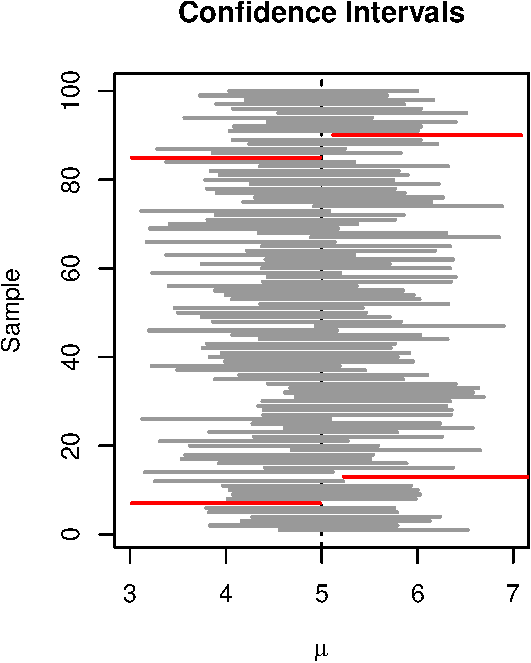
\includegraphics{ITER_files/figure-latex/unnamed-chunk-207-1} \end{center}

For the first \(100\) samples, the true null hypothesis is rejected in
four cases so these intervals do not cover \(\mu=5\). We have indicated
the intervals which lead to a rejection of the null red.

Let us now come back to the example of test scores and class sizes. The
regression model from Chapter \ref{lrwor} is stored in
\texttt{linear\_model}. An easy way to get \(95\%\) confidence intervals
for \(\beta_0\) and \(\beta_1\), the coefficients on
\texttt{(intercept)} and \texttt{STR}, is to use the function
\texttt{confint()}. We only have to provide a fitted model object as an
input to this function. The confidence level is set to \(95\%\) by
default but can be modified by setting the argument \texttt{level}, see
\texttt{?confint}.

\begin{Shaded}
\begin{Highlighting}[]
\CommentTok{# compute 95% confidence interval for coefficients in 'linear_model'}
\KeywordTok{confint}\NormalTok{(linear_model)}
\end{Highlighting}
\end{Shaded}

\begin{verbatim}
##                 2.5 %     97.5 %
## (Intercept) 680.32312 717.542775
## STR          -3.22298  -1.336636
\end{verbatim}

Let us check if the calculation is done as we expect it to be for
\(\beta_1\), the coefficient on \texttt{STR}.

\begin{Shaded}
\begin{Highlighting}[]
\CommentTok{# compute 95% confidence interval for coefficients in 'linear_model' by hand}
\NormalTok{lm_summ <-}\StringTok{ }\KeywordTok{summary}\NormalTok{(linear_model)}

\KeywordTok{c}\NormalTok{(}\StringTok{"lower"}\NormalTok{ =}\StringTok{ }\NormalTok{lm_summ}\OperatorTok{$}\NormalTok{coef[}\DecValTok{2}\NormalTok{,}\DecValTok{1}\NormalTok{] }\OperatorTok{-}\StringTok{ }\KeywordTok{qt}\NormalTok{(}\FloatTok{0.975}\NormalTok{, }\DataTypeTok{df =}\NormalTok{ lm_summ}\OperatorTok{$}\NormalTok{df[}\DecValTok{2}\NormalTok{]) }\OperatorTok{*}\StringTok{ }\NormalTok{lm_summ}\OperatorTok{$}\NormalTok{coef[}\DecValTok{2}\NormalTok{, }\DecValTok{2}\NormalTok{],}
  \StringTok{"upper"}\NormalTok{ =}\StringTok{ }\NormalTok{lm_summ}\OperatorTok{$}\NormalTok{coef[}\DecValTok{2}\NormalTok{,}\DecValTok{1}\NormalTok{] }\OperatorTok{+}\StringTok{ }\KeywordTok{qt}\NormalTok{(}\FloatTok{0.975}\NormalTok{, }\DataTypeTok{df =}\NormalTok{ lm_summ}\OperatorTok{$}\NormalTok{df[}\DecValTok{2}\NormalTok{]) }\OperatorTok{*}\StringTok{ }\NormalTok{lm_summ}\OperatorTok{$}\NormalTok{coef[}\DecValTok{2}\NormalTok{, }\DecValTok{2}\NormalTok{])}
\end{Highlighting}
\end{Shaded}

\begin{verbatim}
##     lower     upper 
## -3.222980 -1.336636
\end{verbatim}

The upper and the lower bounds coincide. We have used the
\(0.975\)-quantile of the \(t_{418}\) distribution to get the exact
result reported by \texttt{confint}. Obviously, this interval \emph{does
not} contain the value zero which, as we have already seen in the
previous section, leads to the rejection of the null hypothesis
\(\beta_{1,0} = 0\).

\section{Regression when X is a Binary Variable}\label{rwxiabv}

Instead of using a continuous regressor \(X\), we might be interested in
running the regression

\[ Y_i = \beta_0 + \beta_1 D_i + u_i \tag{5.2} \]

where \(D_i\) is a binary variable, a so-called \emph{dummy variable}.
For example, we may define \(D_i\) as follows:

\[ D_i = \begin{cases}
        1 \ \ \text{if $STR$ in $i^{th}$ school district < 20} \\
        0 \ \ \text{if $STR$ in $i^{th}$ school district $\geq$ 20} \\
      \end{cases} \tag{5.3} \]

The regression model now is

\[ TestScore_i = \beta_0 + \beta_1 D_i + u_i. \tag{5.4} \]

Let us see how these data look like in a scatter plot:

\begin{Shaded}
\begin{Highlighting}[]
\CommentTok{# Create the dummy variable as defined above}
\NormalTok{CASchools}\OperatorTok{$}\NormalTok{D <-}\StringTok{ }\NormalTok{CASchools}\OperatorTok{$}\NormalTok{STR }\OperatorTok{<}\StringTok{ }\DecValTok{20}

\CommentTok{# Plot the data}
\KeywordTok{plot}\NormalTok{(CASchools}\OperatorTok{$}\NormalTok{D, CASchools}\OperatorTok{$}\NormalTok{score,            }\CommentTok{# provide the data to be plotted}
     \DataTypeTok{pch =} \DecValTok{20}\NormalTok{,                                }\CommentTok{# use filled circles as plot symbols}
     \DataTypeTok{cex =} \FloatTok{0.5}\NormalTok{,                               }\CommentTok{# set size of plot symbols to 0.5}
     \DataTypeTok{col =} \StringTok{"Steelblue"}\NormalTok{,                       }\CommentTok{# set the symbols' color to "Steelblue"}
     \DataTypeTok{xlab =} \KeywordTok{expression}\NormalTok{(D[i]),                 }\CommentTok{# Set title and axis names}
     \DataTypeTok{ylab =} \StringTok{"Test Score"}\NormalTok{,}
     \DataTypeTok{main =} \StringTok{"Dummy Regression"}\NormalTok{)}
\end{Highlighting}
\end{Shaded}

\begin{center}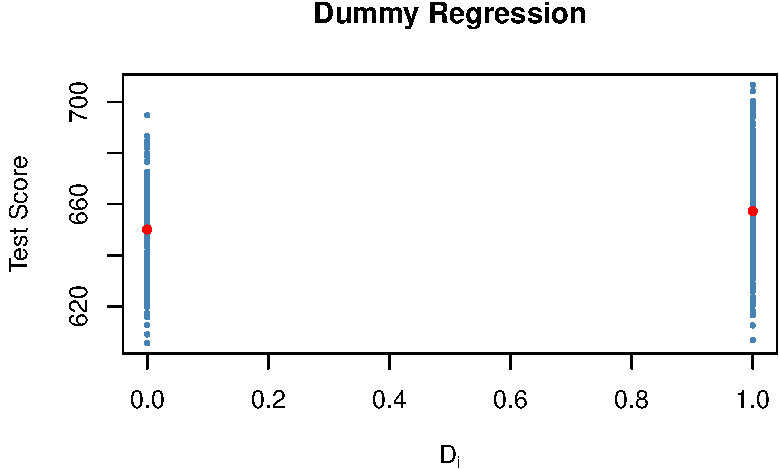
\includegraphics{ITER_files/figure-latex/unnamed-chunk-211-1} \end{center}

With \(D\) as the regressor, it is not useful to think of \(\beta_1\) as
a slope parameter since \(D_i \in \{0,1\}\), i.e., we only observe two
discrete values instead of a continuum of regressor values. There is no
continuous line depicting the conditional expectation function
\(E(TestScore_i | D_i)\) since this function is solely defined for
\(x\)-positions \(0\) and \(1\).

Therefore, the interpretation of the coefficients in this regression
model is as follows:

\begin{itemize}
\item
  \(E(Y_i | D_i = 0) = \beta_0\), so \(\beta_0\) is the expected test
  score in districts where \(D_i=0\) where \(STR\) is below \(20\).
\item
  \(E(Y_i | D_i = 1) = \beta_0 + \beta_1\) or, using the result above,
  \(\beta_1 = E(Y_i | D_i = 1) - E(Y_i | D_i = 0)\). Thus, \(\beta_1\)
  is \emph{the difference in group specific expectations}, i.e., the
  difference in expected test score between districts with \(STR < 20\)
  and those with \(STR \geq 20\).
\end{itemize}

We will now use \texttt{R} to estimate the dummy regression model as
defined by the equations (5.2) and (5.3) .

\begin{Shaded}
\begin{Highlighting}[]
\CommentTok{# estimate the dummy regression model}
\NormalTok{dummy_model <-}\StringTok{ }\KeywordTok{lm}\NormalTok{(score }\OperatorTok{~}\StringTok{ }\NormalTok{D, }\DataTypeTok{data =}\NormalTok{ CASchools)}
\KeywordTok{summary}\NormalTok{(dummy_model)}
\end{Highlighting}
\end{Shaded}

\begin{verbatim}
## 
## Call:
## lm(formula = score ~ D, data = CASchools)
## 
## Residuals:
##     Min      1Q  Median      3Q     Max 
## -50.496 -14.029  -0.346  12.884  49.504 
## 
## Coefficients:
##             Estimate Std. Error t value Pr(>|t|)    
## (Intercept)  650.077      1.393 466.666  < 2e-16 ***
## DTRUE          7.169      1.847   3.882  0.00012 ***
## ---
## Signif. codes:  0 '***' 0.001 '**' 0.01 '*' 0.05 '.' 0.1 ' ' 1
## 
## Residual standard error: 18.74 on 418 degrees of freedom
## Multiple R-squared:  0.0348, Adjusted R-squared:  0.0325 
## F-statistic: 15.07 on 1 and 418 DF,  p-value: 0.0001202
\end{verbatim}

\BeginKnitrBlock{rmdnote}
summary() reports the \(p\)-value of the test that the coefficient on
(Intercept) is zero to to be \textless{} 2e-16. This scientific notation
states that the \(p\)-value is smaller than \(\frac{2}{10^{16}}\), so a
very small number. The reason for this is that computers cannot handle
arbitrary small numbers. In fact, \(\frac{2}{10^{16}}\) is the smallest
possble number R can work with.
\EndKnitrBlock{rmdnote}

The vector \texttt{CASchools\textbackslash{}\$D} has the type
\texttt{logical} (to see this, use \texttt{typeof(CASchools\$D)}) which
is shown in the output of \texttt{summary(dummy\_model)}: the label
\texttt{DTRUE} states that all entries \texttt{TRUE} are coded as
\texttt{1} and all entries \texttt{FALSE} are coded as \texttt{0}. Thus,
the interpretation of the coefficient \texttt{DTRUE} is as stated above
for \(\beta_1\).

One can see that the expected test score in districts with \(STR < 20\)
(\(D_i = 1\)) is predicted to be \(650.1 + 7.17 = 657.27\) while
districts with \(STR \geq 20\) (\(D_i = 0\)) are expected to have an
average test score of only \(650.1\).

Group specific predictions can be added to the plot by execution of the
following code chunk.

\begin{Shaded}
\begin{Highlighting}[]
\CommentTok{# add group specific predictions to the plot}
\KeywordTok{points}\NormalTok{(}\DataTypeTok{x =}\NormalTok{ CASchools}\OperatorTok{$}\NormalTok{D, }
       \DataTypeTok{y =} \KeywordTok{predict}\NormalTok{(dummy_model), }
       \DataTypeTok{col =} \StringTok{"red"}\NormalTok{, }
       \DataTypeTok{pch =} \DecValTok{20}\NormalTok{)}
\end{Highlighting}
\end{Shaded}

Here we use the function \texttt{predict()} to obtain estimates of the
group specific means. The red dots represent these sample group
averages. Accordingly, \(\hat{\beta}_1 = 7.17\) can be seen as the
difference in group averages.

\texttt{summary(dummy\_model)} also answers the question whether there
is a statistically significant difference in group means. This in turn
would support the hypothesis that students perform differently when they
are taught in small classes. We can assess this by a two-tailed test of
the hypothesis \(H_0: \beta_1 = 0\). Conveniently, the \(t\)-statistic
and the corresponding \(p\)-value for this test are computed by
\texttt{summary()}.

Since \texttt{t value} \(= 3.88 > 1.96\) we reject the null hypothesis
at the \(5\%\) level of significance. The same conclusion results when
using the \(p\)-value, which reports significance up to the
\(0.00012\%\) level.

As done with \texttt{linear\_model}, we may alternatively use the
function \texttt{confint()} to compute a \(95\%\) confidence interval
for the true difference in means and see if the hypothesized value is an
element of this confidence set.

\begin{Shaded}
\begin{Highlighting}[]
\CommentTok{# confidence intervals for coefficients in the dummy regression model}
\KeywordTok{confint}\NormalTok{(dummy_model)}
\end{Highlighting}
\end{Shaded}

\begin{verbatim}
##                  2.5 %    97.5 %
## (Intercept) 647.338594 652.81500
## DTRUE         3.539562  10.79931
\end{verbatim}

We reject the hypothesis that there is no difference between group means
at the \(5\%\) significance level since \(\beta_{1,0} = 0\) lies outside
of \([3.54, 10.8]\), the \(95\%\) confidence interval for the
coefficient on \(D\).

\section{Heteroskedasticity and Homoskedasticity}\label{hah}

All inference made in the previous chapters relies on the assumption
that the error variance does not vary as regressor values change. But
this will often not be the case in empirical applications.

\begin{keyconcepts}[Heteroskedasticity and Homoskedasticity]{5.4}
\begin{itemize}
\item The error term of our regression model is homoskedastic if the variance of the conditional distribution of $u_i$ given $X_i$, $Var(u_i|X_i=x)$, is constant \textit{for all} observations in our sample:
\[ \text{Var}(u_i|X_i=x) = \sigma^2 \ \forall \ i=1,\dots,n. \]

\item If instead there is dependence of the conditional variance of $u_i$ on $X_i$, the error term is said to be heteroskedastic. We then write
\[ \text{Var}(u_i|X_i=x) = \sigma_i^2 \ \forall \ i=1,\dots,n. \]

\item Homoskedasticity is a \textit{special case} of heteroskedasticity.
\end{itemize}
\end{keyconcepts}

For a better understanding of heteroskedasticity, we generate some
bivariate heteroskedastic data, estimate a linear regression model and
then use box plots to depict the conditional distributions of the
residuals.

\begin{Shaded}
\begin{Highlighting}[]
\CommentTok{# load scales package for adjusting color opacities}
\KeywordTok{library}\NormalTok{(scales)}

\CommentTok{# generate some heteroskedastic data:}

\CommentTok{# set seed for reproducibility}
\KeywordTok{set.seed}\NormalTok{(}\DecValTok{123}\NormalTok{) }

\CommentTok{# set up vector of x coordinates}
\NormalTok{x <-}\StringTok{ }\KeywordTok{rep}\NormalTok{(}\KeywordTok{c}\NormalTok{(}\DecValTok{10}\NormalTok{, }\DecValTok{15}\NormalTok{, }\DecValTok{20}\NormalTok{, }\DecValTok{25}\NormalTok{), }\DataTypeTok{each =} \DecValTok{25}\NormalTok{)}

\CommentTok{# initialize vector of errors}
\NormalTok{e <-}\StringTok{ }\KeywordTok{c}\NormalTok{()}

\CommentTok{# sample 100 errors such that the variance increases with x}
\NormalTok{e[}\DecValTok{1}\OperatorTok{:}\DecValTok{25}\NormalTok{] <-}\StringTok{ }\KeywordTok{rnorm}\NormalTok{(}\DecValTok{25}\NormalTok{, }\DataTypeTok{sd =} \DecValTok{10}\NormalTok{)}
\NormalTok{e[}\DecValTok{26}\OperatorTok{:}\DecValTok{50}\NormalTok{] <-}\StringTok{ }\KeywordTok{rnorm}\NormalTok{(}\DecValTok{25}\NormalTok{, }\DataTypeTok{sd =} \DecValTok{15}\NormalTok{)}
\NormalTok{e[}\DecValTok{51}\OperatorTok{:}\DecValTok{75}\NormalTok{] <-}\StringTok{ }\KeywordTok{rnorm}\NormalTok{(}\DecValTok{25}\NormalTok{, }\DataTypeTok{sd =} \DecValTok{20}\NormalTok{)}
\NormalTok{e[}\DecValTok{76}\OperatorTok{:}\DecValTok{100}\NormalTok{] <-}\StringTok{ }\KeywordTok{rnorm}\NormalTok{(}\DecValTok{25}\NormalTok{, }\DataTypeTok{sd =} \DecValTok{25}\NormalTok{)}

\CommentTok{# set up y}
\NormalTok{y <-}\StringTok{ }\DecValTok{720} \OperatorTok{-}\StringTok{ }\FloatTok{3.3} \OperatorTok{*}\StringTok{ }\NormalTok{x }\OperatorTok{+}\StringTok{ }\NormalTok{e}

\CommentTok{# Estimate the model }
\NormalTok{mod <-}\StringTok{ }\KeywordTok{lm}\NormalTok{(y }\OperatorTok{~}\StringTok{ }\NormalTok{x)}

\CommentTok{# Plot the data}
\KeywordTok{plot}\NormalTok{(}\DataTypeTok{x =}\NormalTok{ x, }
     \DataTypeTok{y =}\NormalTok{ y, }
     \DataTypeTok{main =} \StringTok{"An Example of Heteroskedasticity"}\NormalTok{,}
     \DataTypeTok{xlab =} \StringTok{"Student-Teacher Ratio"}\NormalTok{,}
     \DataTypeTok{ylab =} \StringTok{"Test Score"}\NormalTok{,}
     \DataTypeTok{cex =} \FloatTok{0.5}\NormalTok{, }
     \DataTypeTok{pch =} \DecValTok{19}\NormalTok{, }
     \DataTypeTok{xlim =} \KeywordTok{c}\NormalTok{(}\DecValTok{8}\NormalTok{, }\DecValTok{27}\NormalTok{), }
     \DataTypeTok{ylim =} \KeywordTok{c}\NormalTok{(}\DecValTok{600}\NormalTok{, }\DecValTok{710}\NormalTok{))}

\CommentTok{# Add the regression line to the plot}
\KeywordTok{abline}\NormalTok{(mod, }\DataTypeTok{col =} \StringTok{"darkred"}\NormalTok{)}

\CommentTok{# Add boxplots to the plot}
\KeywordTok{boxplot}\NormalTok{(}\DataTypeTok{formula =}\NormalTok{ y }\OperatorTok{~}\StringTok{ }\NormalTok{x, }
        \DataTypeTok{add =} \OtherTok{TRUE}\NormalTok{, }
        \DataTypeTok{at =} \KeywordTok{c}\NormalTok{(}\DecValTok{10}\NormalTok{, }\DecValTok{15}\NormalTok{, }\DecValTok{20}\NormalTok{, }\DecValTok{25}\NormalTok{), }
        \DataTypeTok{col =} \KeywordTok{alpha}\NormalTok{(}\StringTok{"gray"}\NormalTok{, }\FloatTok{0.4}\NormalTok{), }
        \DataTypeTok{border =} \StringTok{"black"}
\NormalTok{        )}
\end{Highlighting}
\end{Shaded}

\begin{center}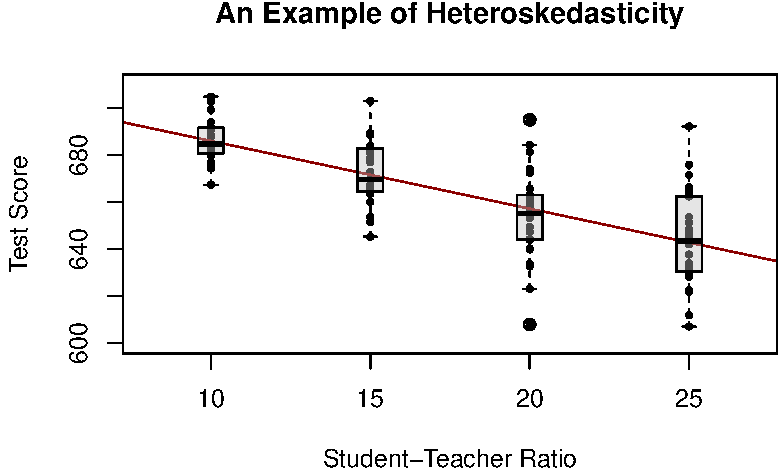
\includegraphics{ITER_files/figure-latex/unnamed-chunk-217-1} \end{center}

We have used the \texttt{formula} argument
\texttt{y \textasciitilde{} x} in \texttt{boxplot()} to specify that we
want to split up the vector \texttt{y} into groups according to
\texttt{x}. \texttt{boxplot(y \textasciitilde{} x)} generates a boxplot
for each of the groups in \texttt{y} defined by \texttt{x}.

For this artificial data it is clear that the conditional error
variances differ. Specifically, we observe that the variance in test
scores (and therefore the variance of the errors committed)
\emph{increases} with the student teacher ratio.

\subsection*{A Real-World Example for
Heteroskedasticity}\label{a-real-world-example-for-heteroskedasticity}
\addcontentsline{toc}{subsection}{A Real-World Example for
Heteroskedasticity}

Think about the economic value of education: if there were no expected
economic value-added to receiving university education, you probably
would not be reading this script right now. A starting point to
empirically verify such a relation is to have data on working
individuals. More precisely, we need data on wages and education of
workers in order to estimate a model like

\[ wage_i = \beta_0 + \beta_1 \cdot education_i + u_i. \]

What can be presumed about this relation? It is likely that, on average,
higher educated workers earn more than workers with less education, so
we expect to estimate an upward sloping regression line. Also, it seems
plausible that earnings of better educated workers have a higher
dispersion then those of low-skilled workers: solid education is not a
guarantee for a high salary so even highly qualified workers take on
low-income jobs. However, they are more likely to meet the requirements
for the well-paid jobs than workers with less education for whom
opportunities in the labor market are much more limited.

To verify this empirically we may use real data on hourly earnings and
the number of years of education of employees. Such data can be found in
\texttt{CPSSWEducation}. This data set is part of the package
\texttt{AER} and comes from the Current Population Survey (CPS) which is
conducted periodically by the \href{http://www.bls.gov/}{Bureau of Labor
Statistics} in the United States.

The subsequent code chunks demonstrate how to import the data into
\texttt{R} and how to produce a plot in the fashion of Figure 5.3 in the
book.

\begin{Shaded}
\begin{Highlighting}[]
\CommentTok{# load package and attach data}
\KeywordTok{library}\NormalTok{(AER)}
\KeywordTok{data}\NormalTok{(}\StringTok{"CPSSWEducation"}\NormalTok{)}
\KeywordTok{attach}\NormalTok{(CPSSWEducation)}

\CommentTok{# get an overview}
\KeywordTok{summary}\NormalTok{(CPSSWEducation)}
\end{Highlighting}
\end{Shaded}

\begin{verbatim}
##       age          gender        earnings        education    
##  Min.   :29.0   female:1202   Min.   : 2.137   Min.   : 6.00  
##  1st Qu.:29.0   male  :1748   1st Qu.:10.577   1st Qu.:12.00  
##  Median :29.0                 Median :14.615   Median :13.00  
##  Mean   :29.5                 Mean   :16.743   Mean   :13.55  
##  3rd Qu.:30.0                 3rd Qu.:20.192   3rd Qu.:16.00  
##  Max.   :30.0                 Max.   :97.500   Max.   :18.00
\end{verbatim}

\begin{Shaded}
\begin{Highlighting}[]
\CommentTok{# estimate a simple regression model}
\NormalTok{labor_model <-}\StringTok{ }\KeywordTok{lm}\NormalTok{(earnings }\OperatorTok{~}\StringTok{ }\NormalTok{education)}

\CommentTok{# plot observations and add the regression line}
\KeywordTok{plot}\NormalTok{(education, }
\NormalTok{     earnings, }
     \DataTypeTok{ylim =} \KeywordTok{c}\NormalTok{(}\DecValTok{0}\NormalTok{, }\DecValTok{150}\NormalTok{))}

\KeywordTok{abline}\NormalTok{(labor_model, }
       \DataTypeTok{col =} \StringTok{"steelblue"}\NormalTok{, }
       \DataTypeTok{lwd =} \DecValTok{2}\NormalTok{)}
\end{Highlighting}
\end{Shaded}

\begin{center}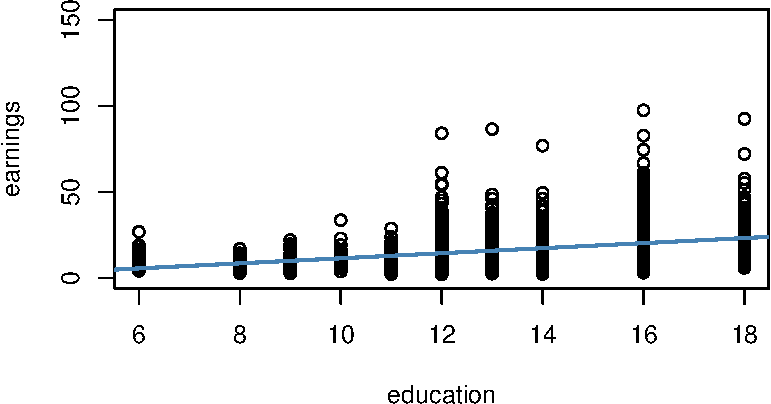
\includegraphics{ITER_files/figure-latex/unnamed-chunk-218-1} \end{center}

The plot reveals that the mean of the distribution of earnings increases
with the level of education. This is also supported by a formal
analysis: the estimated regression model stored in \texttt{labor\_mod}
shows that there is a positive relation between years of education and
earnings.

\begin{Shaded}
\begin{Highlighting}[]
\CommentTok{# print the contents of labor_model to the console}
\NormalTok{labor_model}
\end{Highlighting}
\end{Shaded}

\begin{verbatim}
## 
## Call:
## lm(formula = earnings ~ education)
## 
## Coefficients:
## (Intercept)    education  
##      -3.134        1.467
\end{verbatim}

The estimated regression equation states that, on average, an additional
year of education increases a worker's hourly earnings by about
\(\$ 1.47\). Once more we use \texttt{confint()} to obtain a \(95\%\)
confidence interval for both regression coefficients.

\begin{Shaded}
\begin{Highlighting}[]
\CommentTok{# compute a 95% confidence interval for the coefficients in the model}
\KeywordTok{confint}\NormalTok{(labor_model)}
\end{Highlighting}
\end{Shaded}

\begin{verbatim}
##                 2.5 %    97.5 %
## (Intercept) -5.015248 -1.253495
## education    1.330098  1.603753
\end{verbatim}

Since the interval is \([1.33, 1.60]\) we can reject the hypothesis that
the coefficient on \texttt{education} is zero at the \(5\%\) level.

Furthermore, the plot indicates that there is heteroskedasticity: if we
assume the regression line to be a reasonably good representation of the
conditional mean function \(E(earnings_i\vert education_i)\), the
dispersion of hourly earnings around that function clearly increases
with the level of education, i.e., the variance of the distribution of
earnings increases. In other words: the variance of the errors (the
errors made in explaining earnings by education) increases with
education so that the regression errors are heteroskedastic.

This example makes a case that the assumption of homoskedasticity is
doubtful in economic applications. Should we care about
heteroskedasticity? Yes, we should. As explained in the next section,
heteroskedasticity can have serious negative consequences in hypothesis
testing, if we ignore it.

\subsection*{Should We Care About
Heteroskedasticity?}\label{should-we-care-about-heteroskedasticity}
\addcontentsline{toc}{subsection}{Should We Care About
Heteroskedasticity?}

To answer the question whether we should worry about heteroskedasticity
being present, consider the variance of \(\hat\beta_1\) under the
assumption of homoskedasticity. In this case we have

\[ \sigma^2_{\hat\beta_1} = \frac{\sigma^2_u}{n \cdot \sigma^2_X} \tag{5.5} \]

which is a simplified version of the general equation (4.1) presented in
Key Concept 4.4. See Appendix 5.1 of the book for details on the
derivation. \texttt{summary()} estimates (5.5) by

\[ \overset{\sim}{\sigma}^2_{\hat\beta_1} = \frac{SER^2}{\sum_{i=1}^n (X_i - \overline{X})^2} \ \ \text{where} \ \ SER=\frac{1}{n-2} \sum_{i=1}^n \hat u_i^2. \]

Thus \texttt{summary()} estimates the \emph{homoskedasticity-only}
standard error

\[ \sqrt{ \overset{\sim}{\sigma}^2_{\hat\beta_1} } = \sqrt{ \frac{SER^2}{\sum_{i=1}^n(X_i - \overline{X})^2} }. \]

This is in fact an estimator for the standard deviation of the estimator
\(\hat{\beta}_1\) that is \emph{inconsistent} for the true value
\(\sigma^2_{\hat\beta_1}\) when there is heteroskedasticity. The
implication is that \(t\)-statistics computed in the manner of Key
Concept 5.1 do not follow a standard normal distribution, even in large
samples. This issue may invalidate inference when using the previously
treated tools for hypothesis testing: we should be cautious when making
statements about the significance of regression coefficients on the
basis of \(t\)-statistics as computed by \texttt{summary()} or
confidence intervals produced by \texttt{confint()} if it is doubtful
for the assumption of homoskedasticity to hold!

We will now use \texttt{R} to compute the homoskedasticity-only standard
error for \(\hat{\beta}_1\) in the test score regression model
\texttt{linear\_model} by hand and see that it matches the value
produced by \texttt{summary()}.

\begin{Shaded}
\begin{Highlighting}[]
\CommentTok{# Store model summary in 'model'}
\NormalTok{model <-}\StringTok{ }\KeywordTok{summary}\NormalTok{(linear_model)}

\CommentTok{# Extract the standard error of the regression from model summary}
\NormalTok{SER <-}\StringTok{ }\NormalTok{model}\OperatorTok{$}\NormalTok{sigma}

\CommentTok{# Compute the variation in 'size'}
\NormalTok{V <-}\StringTok{ }\NormalTok{(}\KeywordTok{nrow}\NormalTok{(CASchools)}\OperatorTok{-}\DecValTok{1}\NormalTok{) }\OperatorTok{*}\StringTok{ }\KeywordTok{var}\NormalTok{(CASchools}\OperatorTok{$}\NormalTok{STR)}

\CommentTok{# Compute the standard error of the slope parameter's estimator and print it}
\NormalTok{SE.beta_}\FloatTok{1.}\NormalTok{hat <-}\StringTok{ }\KeywordTok{sqrt}\NormalTok{(SER}\OperatorTok{^}\DecValTok{2}\OperatorTok{/}\NormalTok{V)}
\NormalTok{SE.beta_}\FloatTok{1.}\NormalTok{hat}
\end{Highlighting}
\end{Shaded}

\begin{verbatim}
## [1] 0.4798255
\end{verbatim}

\begin{Shaded}
\begin{Highlighting}[]
\CommentTok{# Use logical operators to see if the value computed by hand matches the one provided }
\CommentTok{# in mod$coefficients. Round estimates to four decimal places}
\KeywordTok{round}\NormalTok{(model}\OperatorTok{$}\NormalTok{coefficients[}\DecValTok{2}\NormalTok{, }\DecValTok{2}\NormalTok{], }\DecValTok{4}\NormalTok{) }\OperatorTok{==}\StringTok{ }\KeywordTok{round}\NormalTok{(SE.beta_}\FloatTok{1.}\NormalTok{hat, }\DecValTok{4}\NormalTok{)}
\end{Highlighting}
\end{Shaded}

\begin{verbatim}
## [1] TRUE
\end{verbatim}

Indeed, the estimated values are equal.

\subsection*{Computation of Heteroskedasticity-Robust Standard
Errors}\label{computation-of-heteroskedasticity-robust-standard-errors}
\addcontentsline{toc}{subsection}{Computation of
Heteroskedasticity-Robust Standard Errors}

Consistent estimation of \(\sigma_{\hat{\beta}_1}\) under
heteroskedasticity is granted when the following \emph{robust} estimator
is used.

\[ SE(\hat{\beta}_1) = \sqrt{ \frac{1}{n} \cdot \frac{ \frac{1}{n} \sum_{i=1}^n (X_i - \overline{X})^2 \hat{u}_i^2 }{ \left[ \frac{1}{n} \sum_{i=1}^n (X_i - \overline{X})^2  \right]^2} } \tag{5.6} \]

Standard error estimates computed this way are also referred to as
\href{https://en.wikipedia.org/wiki/Heteroscedasticity-consistent_standard_errors}{Eicker-Huber-White
standard errors}, the most frequently cited paper on this is
\citet{white1980}.

It can be quite cumbersome to do this calculation by hand. Luckily,
there are \texttt{R} function for that purpose. A convenient one named
\texttt{vcovHC()} is part of the package \texttt{sandwich}.\footnote{The
  package \texttt{sandwich} is a dependency of the package \texttt{AER},
  meaning that it is attached automatically if you load \texttt{AER}.}
This function can compute a variety of standard errors. The one brought
forward in (5.6) is computed when the argument \texttt{type} is set to
\texttt{"HC0"}. Most of the examples presented in the book rely on a
slightly different formula which is the default in the statistics
package \emph{STATA}:

\begin{align}
SE(\hat{\beta}_1)_{HC1} = \sqrt{ \frac{1}{n} \cdot \frac{ \frac{1}{n-2} \sum_{i=1}^n (X_i - \overline{X})^2 \hat{u}_i^2 }{ \left[ \frac{1}{n} \sum_{i=1}^n (X_i - \overline{X})^2  \right]^2}} \label{eq:hc1}
\end{align}

The difference is that we multiply by \(\frac{1}{n-2}\) in the numerator
of \eqref{eq:hc1}. This is a degrees of freedom correction and was
considered by \citet{mackinnon1985}. To get \texttt{vcovHC()} to use
\eqref{eq:hc1}, we have to set \texttt{type = "HC1"}.

Let us now compute robust standard error estimates for the coefficients
in \texttt{linear\_model}.

\begin{Shaded}
\begin{Highlighting}[]
\CommentTok{# compute heteroskedasticity-robust standard errors}
\NormalTok{vcov <-}\StringTok{ }\KeywordTok{vcovHC}\NormalTok{(linear_model, }\DataTypeTok{type =} \StringTok{"HC1"}\NormalTok{)}
\NormalTok{vcov}
\end{Highlighting}
\end{Shaded}

\begin{verbatim}
##             (Intercept)        STR
## (Intercept)  107.419993 -5.3639114
## STR           -5.363911  0.2698692
\end{verbatim}

The output of \texttt{vcovHC()} is the variance-covariance matrix of
coefficient estimates. We are interested in the square root of the
diagonal elements of this matrix, i.e., the standard error estimates.

\BeginKnitrBlock{rmdknit}
When we have k \textgreater{} 1 regressors, writing down the equations
for a regression model becomes very messy. A more convinient way to
denote and estimate so-called multiple regression models (see Chapter
\ref{rmwmr}) is by using matrix algebra. This is why functions like
vcovHC() produce matrices. In the simple linear regression model, the
variances and covariances of the estimators can be gathered in the
symmetric variance-covariance matrix

\begin{equation}
\text{Var}
  \begin{pmatrix}
    \hat\beta_0 \\
    \hat\beta_1
  \end{pmatrix} = 
\begin{pmatrix}
  \text{Var}(\hat\beta_0) & \text{Cov}(\hat\beta_0,\hat\beta_1) \\
\text{Cov}(\hat\beta_0,\hat\beta_1) & \text{Var}(\hat\beta_1)
\end{pmatrix},
\end{equation}

so vcovHC() gives us \(\widehat{\text{Var}}(\hat\beta_0)\),
\(\widehat{\text{Var}}(\hat\beta_1)\) and
\(\widehat{\text{Cov}}(\hat\beta_0,\hat\beta_1)\), but most of the time
we are interested in the diagonal elements of the estimated matrix.
\EndKnitrBlock{rmdknit}

\begin{Shaded}
\begin{Highlighting}[]
\CommentTok{# compute the square root of the diagonal elements in vcov}
\NormalTok{robust_se <-}\StringTok{ }\KeywordTok{sqrt}\NormalTok{(}\KeywordTok{diag}\NormalTok{(vcov))}
\NormalTok{robust_se}
\end{Highlighting}
\end{Shaded}

\begin{verbatim}
## (Intercept)         STR 
##  10.3643617   0.5194893
\end{verbatim}

Now assume we want to generate a coefficient summary as provided by
\texttt{summary()} but with \emph{robust} standard errors of the
coefficient estimators, robust \(t\)-statistics and corresponding
\(p\)-values for the regression model \texttt{linear\_model}. This can
be done using \texttt{coeftest()} from the package \texttt{lmtest}, see
\texttt{?coeftest}. Further we specify in the argument \texttt{vcov.}
that \texttt{vcov}, the Eicker-Huber-White estimate of the variance
matrix we have computed before, should be used.

\begin{Shaded}
\begin{Highlighting}[]
\CommentTok{# we invoke the function `coeftest()` on our model}
\KeywordTok{coeftest}\NormalTok{(linear_model, }\DataTypeTok{vcov. =}\NormalTok{ vcov)}
\end{Highlighting}
\end{Shaded}

\begin{verbatim}
## 
## t test of coefficients:
## 
##              Estimate Std. Error t value  Pr(>|t|)    
## (Intercept) 698.93295   10.36436 67.4362 < 2.2e-16 ***
## STR          -2.27981    0.51949 -4.3886 1.447e-05 ***
## ---
## Signif. codes:  0 '***' 0.001 '**' 0.01 '*' 0.05 '.' 0.1 ' ' 1
\end{verbatim}

We see that the values reported in the column \texttt{Std. Error} are
equal those from \texttt{sqrt(diag(vcov))}.

How severe are the implications of using homoskedasticity-only standard
errors in the presence of heteroskedasticity? The answer is: it depends.
As mentioned above we face the risk of drawing wrong conclusions when
conducting significance tests. Let us illustrate this by generating
another example of a heteroskedastic data set and using it to estimate a
simple regression model. We take

\[ Y_i = \beta_1 \cdot X_i + u_i \ \ , \ \ u_i \overset{i.i.d.}{\sim} \mathcal{N}(0,0.36 \cdot X_i^2)  \]

with \(\beta_1=1\) as the data generating process. Clearly, the
assumption of homoskedasticity is violated here since the variance of
the errors is a nonlinear, increasing function of \(X_i\) but the errors
have zero mean and are i.i.d. such that the assumptions made in Key
Concept 4.3 are not violated. As before, we are interested in estimating
\(\beta_1\).

\begin{Shaded}
\begin{Highlighting}[]
\CommentTok{# generate heteroskedastic data }
\NormalTok{X <-}\StringTok{ }\DecValTok{1}\OperatorTok{:}\DecValTok{500}
\NormalTok{Y <-}\StringTok{ }\KeywordTok{rnorm}\NormalTok{(}\DataTypeTok{n =} \DecValTok{500}\NormalTok{, }\DataTypeTok{mean =}\NormalTok{ X, }\DataTypeTok{sd =} \FloatTok{0.6} \OperatorTok{*}\StringTok{ }\NormalTok{X)}

\CommentTok{# estimate a simple regression model}
\NormalTok{reg <-}\StringTok{ }\KeywordTok{lm}\NormalTok{(Y }\OperatorTok{~}\StringTok{ }\NormalTok{X)}
\end{Highlighting}
\end{Shaded}

We plot the data and add the regression line.

\begin{Shaded}
\begin{Highlighting}[]
\CommentTok{# plot the data}
\KeywordTok{plot}\NormalTok{(}\DataTypeTok{x =}\NormalTok{ X, }\DataTypeTok{y =}\NormalTok{ Y, }
     \DataTypeTok{pch =} \DecValTok{19}\NormalTok{, }
     \DataTypeTok{col =} \StringTok{"steelblue"}\NormalTok{, }
     \DataTypeTok{cex =} \FloatTok{0.8}\NormalTok{)}

\CommentTok{# add the regression line to the plot}
\KeywordTok{abline}\NormalTok{(reg, }
       \DataTypeTok{col =} \StringTok{"darkred"}\NormalTok{, }
       \DataTypeTok{lwd =} \FloatTok{1.5}\NormalTok{)}
\end{Highlighting}
\end{Shaded}

\begin{center}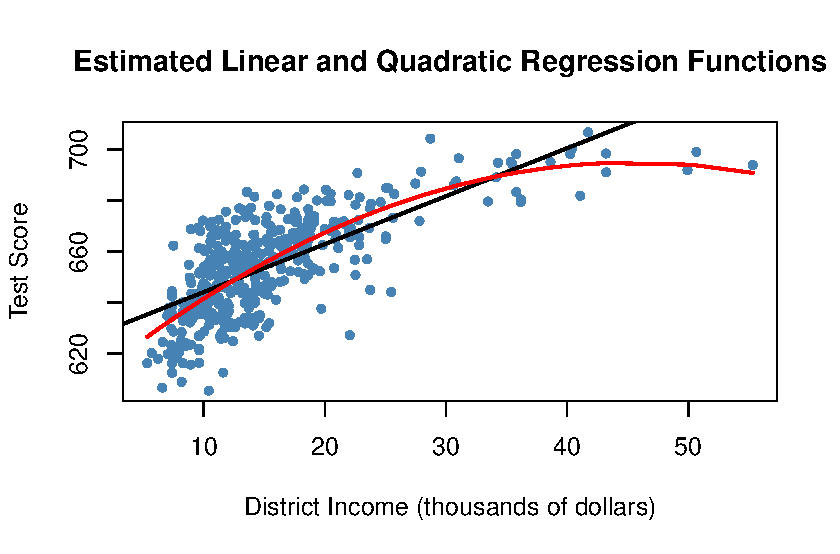
\includegraphics{ITER_files/figure-latex/unnamed-chunk-226-1} \end{center}

The plot shows that the data are heteroskedastic as the variance of
\(Y\) grows with \(X\). We next conduct a significance test of the
(true) null hypothesis \(H_0: \beta_1 = 1\) twice, once using the
homoskedasticity-only standard error formula and once with the robust
version (5.6). An easy way to do this in \texttt{R} is the function
\texttt{linearHypothesis()} from the package \texttt{car}, see
\texttt{?linearHypothesis}. It allows to test linear hypotheses about
parameters in linear models in a similar way as done with a
\(t\)-statistic and offers various robust covariance matrix estimators.
We test by comparing the tests' \(p\)-values to the significance level
of \(5\%\).

\BeginKnitrBlock{rmdknit}
linearHypothesis() computes a test statistic that follows an
\(F\)-distribution under the null hypothesis. We will not loose too much
words on the underlying theory. In general, the idea of the \(F\)-test
is to compare the fit of different models. When testing a hypothesis
about a \emph{single} coefficient using an \(F\)-test, one can show that
the test statistic is simply the square of the corresponding
\(t\)-statistic:

\[F = t^2 = \left(\frac{\hat\beta_i - \beta_{i,0}}{SE(\hat\beta_i)}\right)^2 \sim F_{1,n-k-1}\]

In linearHypothesis(), there are different ways to specify the
hypothesis to be tested, e.g., using a vector of the type character (as
done in the next code chunk), see ?linearHypothesis for alternatives.
The function returns an object of class anova which contains further
information on the test that can be accessed using the \$ operator.
\EndKnitrBlock{rmdknit}

\begin{Shaded}
\begin{Highlighting}[]
\CommentTok{# test hypthesis using the default standard error formula}
\KeywordTok{linearHypothesis}\NormalTok{(reg, }\DataTypeTok{hypothesis.matrix =} \StringTok{"X = 1"}\NormalTok{)}\OperatorTok{$}\StringTok{'Pr(>F)'}\NormalTok{[}\DecValTok{2}\NormalTok{] }\OperatorTok{<}\StringTok{ }\FloatTok{0.05}
\end{Highlighting}
\end{Shaded}

\begin{verbatim}
## [1] TRUE
\end{verbatim}

\begin{Shaded}
\begin{Highlighting}[]
\CommentTok{# test hypothesis using the robust standard error formula}
\KeywordTok{linearHypothesis}\NormalTok{(reg, }\DataTypeTok{hypothesis.matrix =} \StringTok{"X = 1"}\NormalTok{, }\DataTypeTok{white.adjust =} \StringTok{"hc1"}\NormalTok{)}\OperatorTok{$}\StringTok{'Pr(>F)'}\NormalTok{[}\DecValTok{2}\NormalTok{] }\OperatorTok{<}\StringTok{ }\FloatTok{0.05}
\end{Highlighting}
\end{Shaded}

\begin{verbatim}
## [1] FALSE
\end{verbatim}

This is a good example of what can go wrong if we ignore
heteroskedasticity: for the data set at hand the default method rejects
the null hypothesis \(\beta_1 = 1\) although it is true. When using the
robust standard error formula the test does not reject the null. Of
course, we could this might just be a coincidence and both tests do
equally well in maintaining the type I error rate of \(5\%\). This can
be further investigated by computing \emph{Monte Carlo} estimates of the
rejection frequencies of both tests on the basis of a large number of
random samples. We proceed as follows:

\begin{itemize}
\tightlist
\item
  initialize vectors \texttt{t} and \texttt{t.rob}.
\item
  Using a \texttt{for()} loop, we generate \(10000\) heteroskedastic
  random samples of size \(1000\), estimate the regression model and
  check whether the tests falsely reject the null at the level of
  \(5\%\) using comparison operators. The results are stored in the
  respective vectors \texttt{t} and \texttt{t.rob}.
\item
  After the simulation, we compute the fraction of false rejections for
  both tests.
\end{itemize}

\begin{Shaded}
\begin{Highlighting}[]
\CommentTok{# initialize vectors t and t.rob}
\NormalTok{t <-}\StringTok{ }\KeywordTok{c}\NormalTok{()}
\NormalTok{t.rob <-}\StringTok{ }\KeywordTok{c}\NormalTok{()}

\CommentTok{# loop sampling and estimation}
\ControlFlowTok{for}\NormalTok{ (i }\ControlFlowTok{in} \DecValTok{1}\OperatorTok{:}\DecValTok{10000}\NormalTok{) \{}
  
  \CommentTok{# sample data}
\NormalTok{  X <-}\StringTok{ }\DecValTok{1}\OperatorTok{:}\DecValTok{1000}
\NormalTok{  Y <-}\StringTok{ }\KeywordTok{rnorm}\NormalTok{(}\DataTypeTok{n =} \DecValTok{1000}\NormalTok{, }\DataTypeTok{mean =}\NormalTok{ X, }\DataTypeTok{sd =} \FloatTok{0.6}\OperatorTok{*}\NormalTok{X)}

  \CommentTok{# estimate regression model}
\NormalTok{  reg <-}\StringTok{ }\KeywordTok{lm}\NormalTok{(Y }\OperatorTok{~}\StringTok{ }\NormalTok{X)}

  \CommentTok{# homoskedasdicity-only significance test}
\NormalTok{  t[i] <-}\StringTok{ }\KeywordTok{linearHypothesis}\NormalTok{(reg, }\StringTok{"X = 1"}\NormalTok{)}\OperatorTok{$}\StringTok{'Pr(>F)'}\NormalTok{[}\DecValTok{2}\NormalTok{] }\OperatorTok{<}\StringTok{ }\FloatTok{0.05}

  \CommentTok{# robust significance test}
\NormalTok{  t.rob[i] <-}\StringTok{ }\KeywordTok{linearHypothesis}\NormalTok{(reg, }\StringTok{"X = 1"}\NormalTok{, }\DataTypeTok{white.adjust =} \StringTok{"hc1"}\NormalTok{)}\OperatorTok{$}\StringTok{'Pr(>F)'}\NormalTok{[}\DecValTok{2}\NormalTok{] }\OperatorTok{<}\StringTok{ }\FloatTok{0.05}

\NormalTok{\}}

\CommentTok{# compute the fraction of false rejections}
\KeywordTok{round}\NormalTok{(}\KeywordTok{cbind}\NormalTok{(}\DataTypeTok{t =} \KeywordTok{mean}\NormalTok{(t), }\DataTypeTok{t.rob =} \KeywordTok{mean}\NormalTok{(t.rob)), }\DecValTok{3}\NormalTok{)}
\end{Highlighting}
\end{Shaded}

\begin{verbatim}
##          t t.rob
## [1,] 0.073  0.05
\end{verbatim}

These results reveal the increased risk of falsely rejecting the null
using the homoskedasticity-only standard error for the testing problem
at hand: with the common standard error estimator, \(7.28\%\) of all
tests falsely reject the null hypothesis. In contrast, with the robust
test statistic we are closer to the nominal level of \(5\%\).

\section{The Gauss-Markov Theorem}\label{the-gauss-markov-theorem}

When estimating regression models, we know that the results of the
estimation procedure are random. However, when using unbiased
estimators, at least on average, we estimate the true parameter. When
comparing different unbiased estimators, it is therefore interesting to
know which one has the highest precision: being aware that the
likelihood of estimating the \emph{exact} value of the parameter of
interest is \(0\) in an empirical application, we want to make sure that
the likelihood of obtaining an estimate very close to the true value is
as high as possible. This means we want to use the estimator with the
lowest variance of all unbiased estimators, provided we care about
unbiasedness. The Gauss-Markov theorem states that, in the class of
conditionally unbiased linear estimators, the OLS estimator has this
property under certain conditions.

\begin{keyconcepts}[The Gauss-Markov Theorem for $\hat{\beta}_1$]{5.5}
Suppose that the assumptions made in Key Concept 4.3 hold \textit{and} that the errors are \textit{homoskedastic}. The OLS estimator is the best (in the sense of smallest variance) linear conditionally unbiased estimator (BLUE) in this setting.\newline

Let us have a closer look at what this means:\newline

\begin{itemize}
\item Estimators of $\beta_1$ that are linear functions of the $Y_1, \dots, Y_n$ and that are unbiased conditionally on the regressor $X_1, \dots, X_n$ can be written as \[ \overset{\sim}{\beta}_1 = \sum_{i=1}^n a_i Y_i \] where the $a_i$ are weights that are allowed to depend on the $X_i$ but \textit{not} on the $Y_i$. 

\item We already know that $\overset{\sim}{\beta}_1$ has a sampling distribution: $\overset{\sim}{\beta}_1$ is a linear function of the $Y_i$ which are random variables. If now \[ E(\overset{\sim}{\beta}_1 | X_1, \dots, X_n) = \beta_1, \] $\overset{\sim}{\beta}_1$ is a linear unbiased estimator of $\beta_1$, conditionally on the $X_1, \dots, X_n$.

\item We may ask if $\overset{\sim}{\beta}_1$ is also the \textit{best} estimator in this class, i.e., the most efficient one of all linear conditionally unbiased estimators where most efficient means smallest variance. The weights $a_i$ play an important role here and it turns out that OLS uses just the right weights to have the BLUE property. 
\end{itemize}
\end{keyconcepts}

\subsection*{Simulation Study: BLUE
Estimator}\label{simulation-study-blue-estimator}
\addcontentsline{toc}{subsection}{Simulation Study: BLUE Estimator}

Consider the case of a regression of \(Y_i,\dots,Y_n\) only on a
constant. Here, the \(Y_i\) are assumed to be a random sample from a
population with mean \(\mu\) and variance \(\sigma^2\). The OLS
estimator in this model is simply the sample mean, see Chapter
\ref{potsm}.

\begin{equation}
\hat{\beta}_1 = \sum_{i=1}^n \underbrace{\frac{1}{n}}_{=a_i} Y_i \label{eq:bluemean}
\end{equation}

Clearly, each observation is weighted by

\[a_i = \frac{1}{n}.\]

and we also know that \(\text{Var}(\hat{\beta}_1)=\frac{\sigma^2}{n}\).

We now use \texttt{R} to conduct a simulation study that demonstrates
what happens to the variance of \eqref{eq:bluemean} if different weights
\[ w_i = \frac{1 \pm \epsilon}{n} \] are assigned to either half of the
sample \(Y_1, \dots, Y_n\) instead of using \(\frac{1}{n}\), the OLS
weights.

\begin{Shaded}
\begin{Highlighting}[]
\CommentTok{# set sample size and number of repetitions}
\NormalTok{n <-}\StringTok{ }\DecValTok{100}      
\NormalTok{reps <-}\StringTok{ }\FloatTok{1e5}

\CommentTok{# choose epsilon and create a vector of weights as defined above}
\NormalTok{epsilon <-}\StringTok{ }\FloatTok{0.8}
\NormalTok{w <-}\StringTok{ }\KeywordTok{c}\NormalTok{(}\KeywordTok{rep}\NormalTok{((}\DecValTok{1} \OperatorTok{+}\StringTok{ }\NormalTok{epsilon) }\OperatorTok{/}\StringTok{ }\NormalTok{n, n }\OperatorTok{/}\StringTok{ }\DecValTok{2}\NormalTok{), }
       \KeywordTok{rep}\NormalTok{((}\DecValTok{1} \OperatorTok{-}\StringTok{ }\NormalTok{epsilon) }\OperatorTok{/}\StringTok{ }\NormalTok{n, n }\OperatorTok{/}\StringTok{ }\DecValTok{2}\NormalTok{) )}

\CommentTok{# draw a random sample y_1,...,y_n from the standard normal distribution, }
\CommentTok{# use both estimators 1e5 times and store the result in the vectors 'ols' and }
\CommentTok{# 'weightedestimator'}

\NormalTok{ols <-}\StringTok{ }\KeywordTok{rep}\NormalTok{(}\OtherTok{NA}\NormalTok{, reps)}
\NormalTok{weightedestimator <-}\StringTok{ }\KeywordTok{rep}\NormalTok{(}\OtherTok{NA}\NormalTok{, reps)}

\ControlFlowTok{for}\NormalTok{ (i }\ControlFlowTok{in} \DecValTok{1}\OperatorTok{:}\NormalTok{reps) \{}
  
\NormalTok{  y <-}\StringTok{ }\KeywordTok{rnorm}\NormalTok{(n)}
\NormalTok{  ols[i] <-}\StringTok{ }\KeywordTok{mean}\NormalTok{(y)}
\NormalTok{  weightedestimator[i] <-}\StringTok{ }\KeywordTok{crossprod}\NormalTok{(w, y)}
  
\NormalTok{\}}

\CommentTok{# plot kernel density estimates of the estimators' distributions: }

\CommentTok{# OLS}
\KeywordTok{plot}\NormalTok{(}\KeywordTok{density}\NormalTok{(ols), }
     \DataTypeTok{col =} \StringTok{"purple"}\NormalTok{, }
     \DataTypeTok{lwd =} \DecValTok{3}\NormalTok{, }
     \DataTypeTok{main =} \StringTok{"Density of OLS and Weighted Estimator"}\NormalTok{,}
     \DataTypeTok{xlab =} \StringTok{"Estimates"}\NormalTok{)}

\CommentTok{# weighted}
\KeywordTok{lines}\NormalTok{(}\KeywordTok{density}\NormalTok{(weightedestimator), }
      \DataTypeTok{col =} \StringTok{"steelblue"}\NormalTok{, }
      \DataTypeTok{lwd =} \DecValTok{3}\NormalTok{) }

\CommentTok{# add a dashed line at 0 and add a legend to the plot}
\KeywordTok{abline}\NormalTok{(}\DataTypeTok{v =} \DecValTok{0}\NormalTok{, }\DataTypeTok{lty =} \DecValTok{2}\NormalTok{)}

\KeywordTok{legend}\NormalTok{(}\StringTok{'topright'}\NormalTok{, }
       \KeywordTok{c}\NormalTok{(}\StringTok{"OLS"}\NormalTok{, }\StringTok{"Weighted"}\NormalTok{), }
       \DataTypeTok{col =} \KeywordTok{c}\NormalTok{(}\StringTok{"purple"}\NormalTok{, }\StringTok{"steelblue"}\NormalTok{), }
       \DataTypeTok{lwd =} \DecValTok{3}\NormalTok{)}
\end{Highlighting}
\end{Shaded}

\begin{center}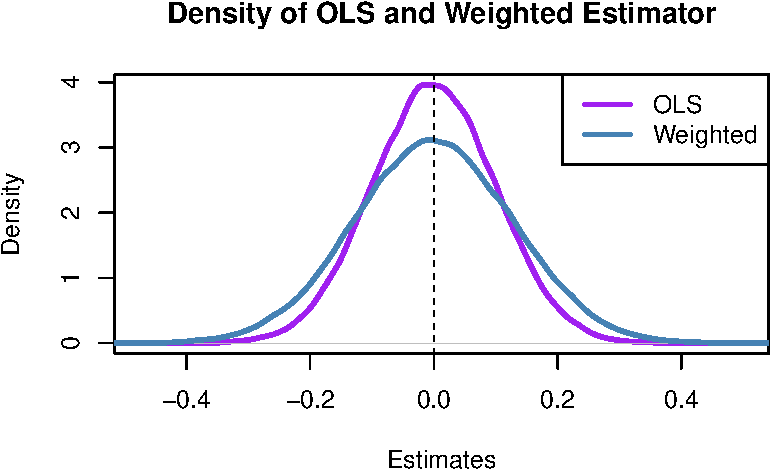
\includegraphics{ITER_files/figure-latex/unnamed-chunk-231-1} \end{center}

What conclusion can we draw from the result?

\begin{itemize}
\tightlist
\item
  Both estimators seem to be unbiased: the means of their estimated
  distributions are zero.
\item
  The estimator using weights that deviate from those implied by OLS is
  less efficient than the OLS estimator: there is higher dispersion when
  weights are \(w_i = \frac{1 \pm 0.8}{100}\) instead of
  \(w_i=\frac{1}{100}\) as required by the OLS solution.
\end{itemize}

Hence, the simulation results support the Gauss-Markov Theorem.

\section{Using the t-Statistic in Regression When the Sample Size Is
Small}\label{using-the-t-statistic-in-regression-when-the-sample-size-is-small}

The three OLS assumptions discussed in Chapter \ref{lrwor} (see Key
Concept 4.3) are the foundation for the results on the large sample
distribution of the OLS estimators in the simple regression model. What
can be said about the distribution of the estimators and their
\(t\)-statistics when the sample size is small and the population
distribution of the data is unknown? Provided that the three least
squares assumptions hold and the errors are normally distributed and
homoskedastic (we refer to these conditions as the homoskedastic normal
regression assumptions), we have normally distributed estimators and
\(t\)-distributed test statistics in small samples.

Recall the \protect\hyperlink{thetdist}{definition} of a
\(t\)-distributed variable

\[ \frac{Z}{\sqrt{W/M}} \sim t_M\]

where \(Z\) is a standard normal random variable, \(W\) is \(\chi^2\)
distributed with \(M\) degrees of freedom and \(Z\) and \(W\) are
independent. See section 5.6 in the book for a more detailed discussion
of the small sample distribution of \(t\)-statistics in regression
methods.

Let us simulate the distribution of regression \(t\)-statistics based on
a large number of small random samples, say \(n=20\), and compare the
simulated distributions to the theoretical distributions which should be
\(t_{18}\), the \(t\)-distribution with \(18\) degrees of freedom
(recall that \(\text{DF}=n-k-1\)).

\begin{Shaded}
\begin{Highlighting}[]
\CommentTok{# initialize two vectors}
\NormalTok{beta_}\DecValTok{0}\NormalTok{ <-}\StringTok{ }\KeywordTok{c}\NormalTok{()}
\NormalTok{beta_}\DecValTok{1}\NormalTok{ <-}\StringTok{ }\KeywordTok{c}\NormalTok{()}

\CommentTok{# loop sampling / estimation / t statistics}
\ControlFlowTok{for}\NormalTok{ (i }\ControlFlowTok{in} \DecValTok{1}\OperatorTok{:}\DecValTok{10000}\NormalTok{) \{}
  
\NormalTok{  X <-}\StringTok{ }\KeywordTok{runif}\NormalTok{(}\DecValTok{20}\NormalTok{, }\DecValTok{0}\NormalTok{, }\DecValTok{20}\NormalTok{)}
\NormalTok{  Y <-}\StringTok{ }\KeywordTok{rnorm}\NormalTok{(}\DataTypeTok{n =} \DecValTok{20}\NormalTok{, }\DataTypeTok{mean =}\NormalTok{ X)}
\NormalTok{  reg <-}\StringTok{ }\KeywordTok{summary}\NormalTok{(}\KeywordTok{lm}\NormalTok{(Y }\OperatorTok{~}\StringTok{ }\NormalTok{X))}
\NormalTok{  beta_}\DecValTok{0}\NormalTok{[i] <-}\StringTok{ }\NormalTok{(reg}\OperatorTok{$}\NormalTok{coefficients[}\DecValTok{1}\NormalTok{, }\DecValTok{1}\NormalTok{] }\OperatorTok{-}\StringTok{ }\DecValTok{0}\NormalTok{)}\OperatorTok{/}\NormalTok{(reg}\OperatorTok{$}\NormalTok{coefficients[}\DecValTok{1}\NormalTok{, }\DecValTok{2}\NormalTok{])}
\NormalTok{  beta_}\DecValTok{1}\NormalTok{[i] <-}\StringTok{ }\NormalTok{(reg}\OperatorTok{$}\NormalTok{coefficients[}\DecValTok{2}\NormalTok{, }\DecValTok{1}\NormalTok{] }\OperatorTok{-}\StringTok{ }\DecValTok{1}\NormalTok{)}\OperatorTok{/}\NormalTok{(reg}\OperatorTok{$}\NormalTok{coefficients[}\DecValTok{2}\NormalTok{, }\DecValTok{2}\NormalTok{])}
  
\NormalTok{\}}

\CommentTok{# plot the distributions and compare with t_18 density:}

\CommentTok{# divide plotting area}
\KeywordTok{par}\NormalTok{(}\DataTypeTok{mfrow =} \KeywordTok{c}\NormalTok{(}\DecValTok{1}\NormalTok{, }\DecValTok{2}\NormalTok{))}

\CommentTok{# plot the simulated density of beta_0}
\KeywordTok{plot}\NormalTok{(}\KeywordTok{density}\NormalTok{(beta_}\DecValTok{0}\NormalTok{), }
     \DataTypeTok{lwd =} \DecValTok{2}\NormalTok{ , }
     \DataTypeTok{main =} \KeywordTok{expression}\NormalTok{(}\KeywordTok{widehat}\NormalTok{(beta)[}\DecValTok{0}\NormalTok{]), }
     \DataTypeTok{xlim =} \KeywordTok{c}\NormalTok{(}\OperatorTok{-}\DecValTok{4}\NormalTok{, }\DecValTok{4}\NormalTok{))}

\CommentTok{# add the t_18 density to the plot}
\KeywordTok{curve}\NormalTok{(}\KeywordTok{dt}\NormalTok{(x, }\DataTypeTok{df =} \DecValTok{18}\NormalTok{), }
      \DataTypeTok{add =}\NormalTok{ T, }
      \DataTypeTok{col =} \StringTok{"red"}\NormalTok{, }
      \DataTypeTok{lwd =} \DecValTok{2}\NormalTok{, }
      \DataTypeTok{lty =} \DecValTok{2}\NormalTok{)}

\CommentTok{# plot the simulated density of beta_1}
\KeywordTok{plot}\NormalTok{(}\KeywordTok{density}\NormalTok{(beta_}\DecValTok{1}\NormalTok{), }
     \DataTypeTok{lwd =} \DecValTok{2}\NormalTok{, }
     \DataTypeTok{main =} \KeywordTok{expression}\NormalTok{(}\KeywordTok{widehat}\NormalTok{(beta)[}\DecValTok{1}\NormalTok{]), }\DataTypeTok{xlim =} \KeywordTok{c}\NormalTok{(}\OperatorTok{-}\DecValTok{4}\NormalTok{, }\DecValTok{4}\NormalTok{)}
\NormalTok{     )}

\CommentTok{# add the t_18 density to the plot}
\KeywordTok{curve}\NormalTok{(}\KeywordTok{dt}\NormalTok{(x, }\DataTypeTok{df =} \DecValTok{18}\NormalTok{), }
      \DataTypeTok{add =}\NormalTok{ T, }
      \DataTypeTok{col =} \StringTok{"red"}\NormalTok{, }
      \DataTypeTok{lwd =} \DecValTok{2}\NormalTok{, }
      \DataTypeTok{lty =} \DecValTok{2}\NormalTok{) }
\end{Highlighting}
\end{Shaded}

\begin{center}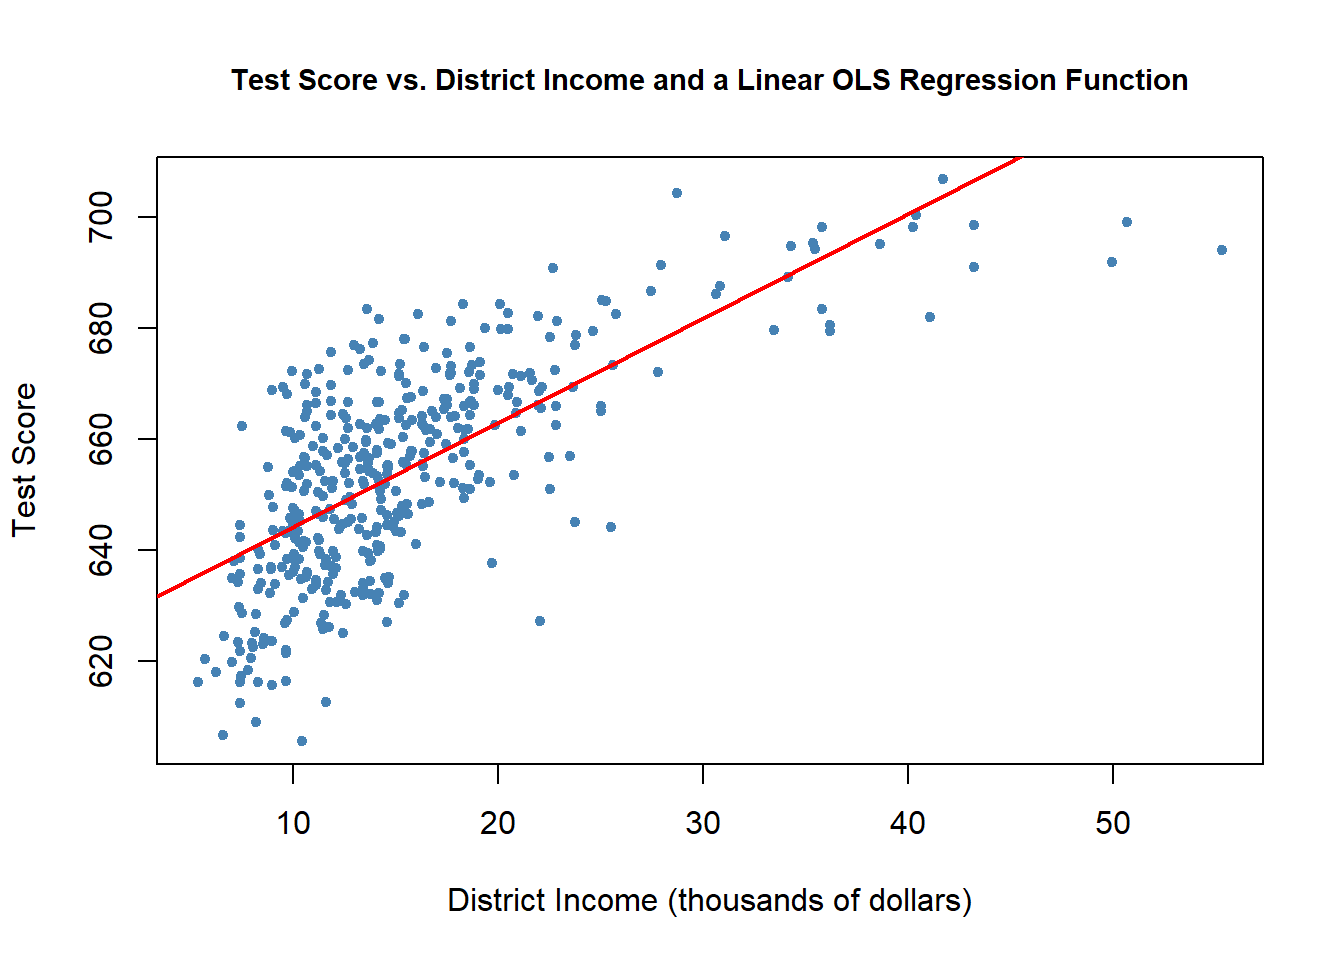
\includegraphics{ITER_files/figure-latex/unnamed-chunk-232-1} \end{center}

The outcomes are consistent with our expectations: the empirical
distributions of both estimators seem to track the theoretical
\(t_{18}\) distribution quite closely.

\section{Exercises}\label{exercises-3}

\begin{center}\textit{This interactive part of the book is only available in the HTML version.}\end{center}

\chapter{Regression Models with Multiple Regressors}\label{rmwmr}

In what follows we introduce linear regression models that use more than
just one explanatory variable and discuss important key concepts in
multiple regression. As we broaden our scope beyond the relationship of
only two variables (the dependent variable and a single regressor) some
potential new issues arise such as \emph{multicollinearity} and
\emph{omitted variable bias} (OVB). In particular, this chapter deals
with omitted variables and its implication for causal interpretation of
OLS-estimated coefficients.

Naturally, we will discuss estimation of multiple regression models
using \texttt{R}. We will also illustrate the importance of thoughtful
usage of multiple regression models via simulation studies that
demonstrate the consequences of using highly correlated regressors or
misspecified models.

The packages \texttt{AER} \citep{R-AER} and \texttt{MASS} \citep{R-MASS}
are needed for reproducing the code presented in this chapter. Make sure
that the following code chunk executes without any errors.

\begin{Shaded}
\begin{Highlighting}[]
\KeywordTok{library}\NormalTok{(AER)}
\KeywordTok{library}\NormalTok{(MASS)}
\end{Highlighting}
\end{Shaded}

\section{Omitted Variable Bias}\label{omitted-variable-bias}

The previous analysis of the relationship between test score and class
size discussed in Chapters \ref{lrwor} and \ref{htaciitslrm} has a major
flaw: we ignored other determinants of the dependent variable (test
score) that correlate with the regressor (class size). Remember that
influences on the dependent variable which are not captured by the model
are collected in the error term, which we so far assumed to be
uncorrelated with the regressor. However, this assumption is violated if
we exclude determinants of the dependent variable which vary with the
regressor. This might induce an estimation bias, i.e., the mean of the
OLS estimator's sampling distribution is no longer equals the true mean.
In our example we therefore wrongly estimate the causal effect on test
scores of a unit change in the student-teacher ratio, on average. This
issue is called \emph{omitted variable bias} (OVB) and is summarized by
Key Concept 6.1.

\begin{keyconcepts}[Omitted Variable Bias in Regression with a Single Regressor]{6.1}
Omitted variable bias is the bias in the OLS estimator that arises when the regressor, $X$, is \textit{correlated} with an omitted variable. For omitted variable bias to occur, two conditions must be fulfilled:\newline

\begin{enumerate}
\item $X$ is correlated with the omitted variable. 
\item The omitted variable is a determinant of the dependent variable $Y$.
\end{enumerate}\vspace{0.5cm}

Together, 1. and 2. result in a violation of the first OLS assumption $E(u_i\vert X_i) = 0$. Formally, the resulting bias can be expressed as

\begin{align}
\hat\beta_1 \xrightarrow[]{p} \beta_1 + \rho_{Xu} \frac{\sigma_u}{\sigma_X}.
\end{align}

See Appendix 6.1 of the book for a detailed derivation. (6.1) states that OVB is a problem that cannot be solved by increasing the number of observations used to estimate $\beta_1$, as $\hat\beta_1$ is inconsistent: OVB prevents the estimator from converging in probability to the true parameter value. Strength and direction of the bias are determined by $\rho_{Xu}$, the correlation between the error term and the regressor.
\end{keyconcepts}

In the example of test score and class size, it is easy to come up with
variables that may cause such a bias, if omitted from the model. As
mentioned in the book, a highly relevant variable could be the
percentage of English learners in the school district: it is plausible
that the ability to speak, read and write English is an important factor
for successful learning. Therefore, students that are still learning
English are likely to perform worse in tests than native speakers. Also,
it is conceivable that the share of English learning students is bigger
in school districts where class sizes are relatively large: think of
poor urban districts where a lot of immigrants live.

Let us think about a possible bias induced by omitting the share of
English learning students (\(PctEL\)) in view of (6.1). When the
estimated regression model does not include \(PctEL\) as a regressor
although the true data generating process (DGP) is

\[ TestScore = \beta_0 + \beta_1 \times STR + \beta_2 \times PctEL \tag{6.2}\]

where \(STR\) and \(PctEL\) are correlated, we have

\[\rho_{STR,PctEL}\neq0.\]

Let us investigate this using \texttt{R}. After defining our variables
we may compute the correlation between \(STR\) and \(PctEL\) as well as
the correlation between \(STR\) and \(TestScore\).

\begin{Shaded}
\begin{Highlighting}[]
\CommentTok{# load the AER package}
\KeywordTok{library}\NormalTok{(AER)}

\CommentTok{# load the data set}
\KeywordTok{data}\NormalTok{(CASchools)   }

\CommentTok{# define variables}
\NormalTok{CASchools}\OperatorTok{$}\NormalTok{STR <-}\StringTok{ }\NormalTok{CASchools}\OperatorTok{$}\NormalTok{students}\OperatorTok{/}\NormalTok{CASchools}\OperatorTok{$}\NormalTok{teachers       }
\NormalTok{CASchools}\OperatorTok{$}\NormalTok{score <-}\StringTok{ }\NormalTok{(CASchools}\OperatorTok{$}\NormalTok{read }\OperatorTok{+}\StringTok{ }\NormalTok{CASchools}\OperatorTok{$}\NormalTok{math)}\OperatorTok{/}\DecValTok{2}

\CommentTok{# compute correlations}
\KeywordTok{cor}\NormalTok{(CASchools}\OperatorTok{$}\NormalTok{STR, CASchools}\OperatorTok{$}\NormalTok{score)}
\end{Highlighting}
\end{Shaded}

\begin{verbatim}
## [1] -0.2263627
\end{verbatim}

\begin{Shaded}
\begin{Highlighting}[]
\KeywordTok{cor}\NormalTok{(CASchools}\OperatorTok{$}\NormalTok{STR, CASchools}\OperatorTok{$}\NormalTok{english)}
\end{Highlighting}
\end{Shaded}

\begin{verbatim}
## [1] 0.1876424
\end{verbatim}

The fact that \(\widehat{\rho}_{STR, Testscore} = -0.2264\) is cause for
concern that omitting \(PctEL\) leads to a negatively biased estimate
\(\hat\beta_1\) since this indicates that \(\rho_{Xu} < 0\). As a
consequence we expect \(\hat\beta_1\), the coefficient on \(STR\), to be
too large in absolute value. Put differently, the OLS estimate of
\(\hat\beta_1\) suggests that small classes improve test scores, but
that the effect of small classes is overestimated as it captures the
effect of having fewer English learners, too.

What happens to the magnitude of \(\hat\beta_1\) if we add the variable
\(PctEL\) to the regression, that is, if we estimate the model
\[ TestScore = \beta_0 + \beta_1 \times STR + \beta_2 \times PctEL + u \]

instead? And what do we expect about the sign of \(\hat\beta_2\), the
estimated coefficient on \(PctEL\)? Following the reasoning above we
should still end up with a negative but larger coefficient estimate
\(\hat\beta_1\) than before and a negative estimate \(\hat\beta_2\).

Let us estimate both regression models and compare. Performing a
multiple regression in \texttt{R} is straightforward. One can simply add
additional variables to the right hand side of the \texttt{formula}
argument of the function \texttt{lm()} by using their names and the
\texttt{+} operator.

\begin{Shaded}
\begin{Highlighting}[]
\CommentTok{# estimate both regression models}
\NormalTok{mod <-}\StringTok{ }\KeywordTok{lm}\NormalTok{(score }\OperatorTok{~}\StringTok{ }\NormalTok{STR, }\DataTypeTok{data =}\NormalTok{ CASchools) }
\NormalTok{mult.mod <-}\StringTok{ }\KeywordTok{lm}\NormalTok{(score }\OperatorTok{~}\StringTok{ }\NormalTok{STR }\OperatorTok{+}\StringTok{ }\NormalTok{english, }\DataTypeTok{data =}\NormalTok{ CASchools)}

\CommentTok{# print the results to the console}
\NormalTok{mod}
\end{Highlighting}
\end{Shaded}

\begin{verbatim}
## 
## Call:
## lm(formula = score ~ STR, data = CASchools)
## 
## Coefficients:
## (Intercept)          STR  
##      698.93        -2.28
\end{verbatim}

\begin{Shaded}
\begin{Highlighting}[]
\NormalTok{mult.mod}
\end{Highlighting}
\end{Shaded}

\begin{verbatim}
## 
## Call:
## lm(formula = score ~ STR + english, data = CASchools)
## 
## Coefficients:
## (Intercept)          STR      english  
##    686.0322      -1.1013      -0.6498
\end{verbatim}

We find the outcomes to be consistent with our expectations.

The following section discusses some theory on multiple regression
models.

\section{The Multiple Regression Model}\label{tmrm}

The multiple regression model extends the basic concept of the simple
regression model discussed in Chapters \ref{lrwor} and
\ref{htaciitslrm}. A multiple regression model enables us to estimate
the effect on \(Y_i\) of changing a regressor \(X_{1i}\) if the
remaining regressors \(X_{2i},X_{3i}\dots,X_{ki}\) \emph{do not vary}.
In fact we already have performed estimation of the multiple regression
model (6.2) using \texttt{R} in the previous section. The interpretation
of the coefficient on student-teacher ratio is the effect on test scores
of a one unit change student-teacher ratio if the percentage of English
learners is kept constant.

Just like in the simple regression model, we assume the true
relationship between \(Y\) and \(X_{1i},X_{2i}\dots\dots,X_{ki}\) to be
linear. On average, this relation is given by the population regression
function

\[ E(Y_i\vert X_{1i}=x_1, X_{2i}=x_2,  X_{3i}=x_3,\dots, X_{ki}=x_k) = \beta_0 + \beta_1 x_1 + \beta_2 x_2 + \beta_3 x_3 + \dots + \beta_k x_k. \tag{6.3} \]

As in the simple regression model, the relation
\[Y_i = \beta_0 + \beta_1 X_{1i} + \beta_2 X_{2i} + \beta_3 X_{3i} + \dots + \beta_k X_{ki}\]
does not hold exactly since there are disturbing influences to the
dependent variable \(Y\) we cannot observe as explanatory variables.
Therefore we add an error term \(u\) which represents deviations of the
observations from the population regression line to (6.3). This yields
the population multiple regression model
\[ Y_i = \beta_0 + \beta_1 X_{1i} + \beta_2 X_{2i} + \beta_3 X_{3i} + \dots + \beta_k X_{ki} + u_i, \ i=1,\dots,n. \tag{6.4} \]

Key Concept 6.2 summarizes the core concepts of the multiple regression
model.

\begin{keyconcepts}[The Multiple Regression Model]{6.2}
\begin{itemize}
\item $Y_i$ is the $i^{th}$ observation in the dependent variable. Observations on the $k$ regressors are denoted by $X_{1i},X_{2i},\dots,X_{ki}$ and $u_i$ is the error term.
\item The average relationship between $Y$ and the regressors is given by the population regression line
$$ E(Y_i\vert X_{1i}=x_1, X_{2i}=x_2,  X_{3i}=x_3,\dots, X_{ki}=x_k) = \beta_0 + \beta_1 x_1 + \beta_2 x_2 + \beta_3 x_3 + \dots + \beta_k x_k. $$
\item $\beta_0$ is the intercept; it is the expected value of $Y$ when all $X$s equal $0$. $\beta_j \ , \ j=1,\dots,k$ are the coefficients on $X_j \ , \ j=1,\dots,k$. $\beta_1$ measures the expected change in $Y_i$ that results from a one unit change in $X_{1i}$ while holding all other regressors constant. 
\end{itemize}
\end{keyconcepts}

How can we estimate the coefficients of the multiple regression model
(6.4)? We will not go too much into detail on this issue as our focus is
on using \texttt{R}. However, it should be pointed out that, similarly
to the simple regression model, the coefficients of the multiple
regression model can be estimated using OLS. As in the simple model, we
seek to minimize the sum of squared mistakes by choosing estimates
\(b_0,b_1,\dots,b_k\) for the coefficients
\(\beta_0,\beta_1,\dots,\beta_k\) such that

\[\sum_{i=1}^n (Y_i - b_0 - b_1 X_{1i} - b_2 X_{2i} - \dots -  b_k X_{ki})^2 \tag{6.5}\]

is minimized. Note that (6.5) is simply an extension of \(SSR\) in the
case with just one regressor and a constant. The estimators that
minimize (6.5) are hence denoted
\(\hat\beta_0,\hat\beta_1,\dots,\hat\beta_k\) and, as in the simple
regression model, we call them the ordinary least squares estimators of
\(\beta_0,\beta_1,\dots,\beta_k\). For the predicted value of \(Y_i\)
given the regressors and the estimates
\(\hat\beta_0,\hat\beta_1,\dots,\hat\beta_k\) we have

\[ \hat{Y}_i = \hat\beta_0 + \hat\beta_1 X_{1i} + \dots +\hat\beta_k X_{ki}. \]
The difference between \(Y_i\) and its predicted value \(\hat{Y}_i\) is
called the OLS residual of observation \(i\):
\(\hat{u} = Y_i - \hat{Y}_i\).

For further information regarding the theory behind multiple regression,
see Chapter 18.1 of the book which inter alia presents a derivation of
the OLS estimator in the multiple regression model using matrix
notation.

Now let us jump back to the example of test scores and class sizes. The
estimated model object is \texttt{mult.mod}. As for simple regression
models we can use \texttt{summary()} to obtain information on estimated
coefficients and model statistics.

\begin{Shaded}
\begin{Highlighting}[]
\KeywordTok{summary}\NormalTok{(mult.mod)}\OperatorTok{$}\NormalTok{coef}
\end{Highlighting}
\end{Shaded}

\begin{verbatim}
##                Estimate Std. Error    t value      Pr(>|t|)
## (Intercept) 686.0322445 7.41131160  92.565565 3.871327e-280
## STR          -1.1012956 0.38027827  -2.896026  3.978059e-03
## english      -0.6497768 0.03934254 -16.515882  1.657448e-47
\end{verbatim}

So the estimated multiple regression model is

\[ \widehat{TestScore} = 686.03 - 1.10 \times STR - 0.65 \times PctEL \tag{6.6}.  \]

Unlike in the simple regression model where the data can be represented
by points in the two-dimensional coordinate system, we now have three
dimensions. Hence observations can be represented by points in
three-dimensional space. Therefore (6.6) is now longer a regression line
but a \emph{regression plane}. This idea extends to higher dimensions
when we further expand the number of regressors \(k\). We then say that
the regression model can be represented by a hyperplane in the \(k+1\)
dimensional space. It is already hard to imagine such a space if \(k=3\)
and we best stick with the general idea that, in the multiple regression
model, the dependent variable is explained by a \emph{linear combination
of the regressors}. However, in the present case we are able to
visualize the situation. The following figure is an interactive 3D
visualization of the data and the estimated regression plane (6.6).

\begin{center}\textit{This interactive part of the book is only available in the HTML version.}\end{center}

We observe that the estimated regression plane fits the data reasonably
well --- at least with regard to the shape and spatial position of the
points. The color of the markers is an indicator for the absolute
deviation from the predicted regression plane. Observations that are
colored more reddish lie close to the regression plane while the color
shifts to blue with growing distance. An anomaly that can be seen from
the plot is that there might be heteroskedasticity: we see that the
dispersion of regression errors made, i.e., the distance of observations
to the regression plane tends to decrease as the share of English
learning students increases.

\section{Measures of Fit in Multiple Regression}\label{mofimr}

In multiple regression, common summary statistics are \(SER\), \(R^2\)
and the adjusted \(R^2\).

Taking the code from Section \ref{tmrm}, simply use
\texttt{summary(mult.mod)} to obtain the \(SER\), \(R^2\) and
adjusted-\(R^2\). For multiple regression models the \(SER\) is computed
as

\[ SER = s_{\hat u} = \sqrt{s_{\hat u}^2} \] where modify the
denominator of the premultiplied factor in \(s_{\hat u}^2\) in order to
accommodate for additional regressors. Thus,

\[ s_{\hat u}^2 = \frac{1}{n-k-1} \, SSR \]

with \(k\) denoting the number of regressors \emph{excluding} the
intercept.

While \texttt{summary()} computes the \(R^2\) just as in the case of a
single regressor, it is no reliable measure for multiple regression
models. This is due to \(R^2\) increasing whenever an additional
regressor is added to the model. Adding a regressor decreases the
\(SSR\) --- at least unless the respective estimated coefficient is
exactly zero what practically never happens (see Chapter 6.4 of the book
for a detailed argument). The adjusted \(R^2\) takes this into
consideration by ``punishing'' the addition of regressors using a
correction factor. So the adjusted \(R^2\), or simply \(\bar{R}^2\), is
a modified version of \(R^2\). It is defined as

\[ \bar{R}^2 = 1-\frac{n-1}{n-k-1} \, \frac{SSR}{TSS}. \]

As you may have already suspected, \texttt{summary()} adjusts the
formula for \(SER\) and it computes \(\bar{R}^2\) and of course \(R^2\)
by default, thereby leaving the decision which measure to rely on to the
user.

You can find both measures at the bottom of the output produced by
calling \texttt{summary(mult.mod)}.

\begin{Shaded}
\begin{Highlighting}[]
\KeywordTok{summary}\NormalTok{(mult.mod)}
\end{Highlighting}
\end{Shaded}

\begin{verbatim}
## 
## Call:
## lm(formula = score ~ STR + english, data = CASchools)
## 
## Residuals:
##     Min      1Q  Median      3Q     Max 
## -48.845 -10.240  -0.308   9.815  43.461 
## 
## Coefficients:
##              Estimate Std. Error t value Pr(>|t|)    
## (Intercept) 686.03224    7.41131  92.566  < 2e-16 ***
## STR          -1.10130    0.38028  -2.896  0.00398 ** 
## english      -0.64978    0.03934 -16.516  < 2e-16 ***
## ---
## Signif. codes:  0 '***' 0.001 '**' 0.01 '*' 0.05 '.' 0.1 ' ' 1
## 
## Residual standard error: 14.46 on 417 degrees of freedom
## Multiple R-squared:  0.4264, Adjusted R-squared:  0.4237 
## F-statistic:   155 on 2 and 417 DF,  p-value: < 2.2e-16
\end{verbatim}

We can also compute the measures by hand using the formulas above. Let
us check that the results coincide with the values provided by
\texttt{summary()}.

\begin{Shaded}
\begin{Highlighting}[]
\CommentTok{# define the components}
\NormalTok{n <-}\StringTok{ }\KeywordTok{nrow}\NormalTok{(CASchools)                            }\CommentTok{# number of observations (rows)}
\NormalTok{k <-}\StringTok{ }\DecValTok{2}                                          \CommentTok{# number of regressors}

\NormalTok{y_mean <-}\StringTok{ }\KeywordTok{mean}\NormalTok{(CASchools}\OperatorTok{$}\NormalTok{score)                 }\CommentTok{# mean of avg. test-scores}

\NormalTok{SSR <-}\StringTok{ }\KeywordTok{sum}\NormalTok{(}\KeywordTok{residuals}\NormalTok{(mult.mod)}\OperatorTok{^}\DecValTok{2}\NormalTok{)               }\CommentTok{# sum of squared residuals}
\NormalTok{TSS <-}\StringTok{ }\KeywordTok{sum}\NormalTok{((CASchools}\OperatorTok{$}\NormalTok{score }\OperatorTok{-}\StringTok{ }\NormalTok{y_mean )}\OperatorTok{^}\DecValTok{2}\NormalTok{)       }\CommentTok{# total sum of squares}
\NormalTok{ESS <-}\StringTok{ }\KeywordTok{sum}\NormalTok{((}\KeywordTok{fitted}\NormalTok{(mult.mod) }\OperatorTok{-}\StringTok{ }\NormalTok{y_mean)}\OperatorTok{^}\DecValTok{2}\NormalTok{)       }\CommentTok{# explained sum of squares}

\CommentTok{# compute the measures}

\NormalTok{SER <-}\StringTok{ }\KeywordTok{sqrt}\NormalTok{(}\DecValTok{1}\OperatorTok{/}\NormalTok{(n}\OperatorTok{-}\NormalTok{k}\OperatorTok{-}\DecValTok{1}\NormalTok{) }\OperatorTok{*}\StringTok{ }\NormalTok{SSR)                    }\CommentTok{# standard error of the regression}
\NormalTok{Rsq <-}\StringTok{ }\DecValTok{1} \OperatorTok{-}\StringTok{ }\NormalTok{(SSR }\OperatorTok{/}\StringTok{ }\NormalTok{TSS)                          }\CommentTok{# R^2}
\NormalTok{adj_Rsq <-}\StringTok{ }\DecValTok{1} \OperatorTok{-}\StringTok{ }\NormalTok{(n}\OperatorTok{-}\DecValTok{1}\NormalTok{)}\OperatorTok{/}\NormalTok{(n}\OperatorTok{-}\NormalTok{k}\OperatorTok{-}\DecValTok{1}\NormalTok{) }\OperatorTok{*}\StringTok{ }\NormalTok{SSR}\OperatorTok{/}\NormalTok{TSS          }\CommentTok{# adj. R^2}

\CommentTok{# print the measures to the console}
\KeywordTok{c}\NormalTok{(}\StringTok{"SER"}\NormalTok{ =}\StringTok{ }\NormalTok{SER, }\StringTok{"R2"}\NormalTok{ =}\StringTok{ }\NormalTok{Rsq, }\StringTok{"Adj.R2"}\NormalTok{ =}\StringTok{ }\NormalTok{adj_Rsq)}
\end{Highlighting}
\end{Shaded}

\begin{verbatim}
##        SER         R2     Adj.R2 
## 14.4644831  0.4264315  0.4236805
\end{verbatim}

Now, what can we say about the fit of our multiple regression model for
test scores with the percentage of English learners as an additional
regressor? Does it improve on the simple model including only an
intercept and a measure of class size? The answer is yes: compare
\(\bar{R}^2\) with that obtained for the simple regression model
\texttt{mod}.

Including \(PctEL\) as a regressor improves the \(\bar{R}^2\), which we
deem to be more reliable in view of the above discussion. Notice that
the difference between \(R^2\) and \(\bar{R}^2\) is small since \(k=2\)
and \(n\) is large. In short, the fit of (6.6) improves vastly on the
fit of the simple regression model with \(STR\) as the only regressor.
Comparing regression errors we find that the precision of the multiple
regression model (6.6) improves upon the simple model as adding
\(PctEL\) lowers the \(SER\) from \(18.6\) to \(14.5\) units of test
score.

As already mentioned, \(\bar{R}^2\) may be used to quantify how good a
model fits the data. However, it is rarely a good idea to maximize these
measures by stuffing the model with regressors. You will not find any
serious study that does so. Instead, it is more useful to include
regressors that improve the estimation of the causal effect of interest
which is \emph{not} assessed by means the \(R^2\) of the model. The
issue of variable selection is covered in Chapter \ref{nrf}.

\section{OLS Assumptions in Multiple
Regression}\label{ols-assumptions-in-multiple-regression}

In the multiple regression model we extend the three least squares
assumptions of the simple regression model (see Chapter \ref{lrwor}) and
add a fourth assumption. These assumptions are presented in Key Concept
6.4. We will not go into the details of assumptions 1-3 since their
ideas generalize easy to the case of multiple regressors. We will focus
on the fourth assumption. This assumption rules out perfect correlation
between regressors.

\begin{keyconcepts}[The Least Squares Assumptions in the Multiple Regression Model]{6.4}
The multiple regression model is given by

$$ Y_i = \beta_0 + \beta_1 X_{1i} + \beta_1 X_{2i} + \dots + \beta_k X_{ki} + u_i \ , \ i=1,\dots,n. $$

The OLS assumptions in the multiple regression model are an extension of the ones made for the simple regression model:\newline

\begin{enumerate}
\item Regressors $(X_{1i}, X_{2i}, \dots, X_{ki}, Y_i) \ , \ i=1,\dots,n$, are drawn such that the i.i.d. assumption holds. 
\item $u_i$ is an error term with conditional mean zero given the regressors, i.e.,
$$ E(u_i\vert X_{1i}, X_{2i}, \dots, X_{ki}) = 0. $$
\item Large outliers are unlikely, formally $X_{1i},\dots,X_{ki}$ and $Y_i$ have finite fourth moments.
\item No perfect multicollinearity.
\end{enumerate}
\end{keyconcepts}

\subsection*{Multicollinearity}\label{multicollinearity}
\addcontentsline{toc}{subsection}{Multicollinearity}

\emph{Multicollinearity} means that two or more regressors in a multiple
regression model are \emph{strongly} correlated. If the correlation
between two or more regressors is perfect, that is, one regressor can be
written as a linear combination of the other(s), we have \emph{perfect
multicollinearity}. While strong multicollinearity in general is
unpleasant as it causes the variance of the OLS estimator to be large
(we will discuss this in more detail later), the presence of perfect
multicollinearity makes it impossible to solve for the OLS estimator,
i.e., the model cannot be estimated in the first place.

The next section presents some examples of perfect multicollinearity and
demonstrates how \texttt{lm()} deals with them.

\subsubsection*{Examples of Perfect
Multicollinearity}\label{examples-of-perfect-multicollinearity}
\addcontentsline{toc}{subsubsection}{Examples of Perfect
Multicollinearity}

How does \texttt{R} react if we try to estimate a model with perfectly
correlated regressors?

\texttt{lm} will produce a warning in the first line of the coefficient
section of the output (\texttt{1 not defined because of singularities})
and ignore the regressor(s) which is (are) assumed to be a linear
combination of the other(s). Consider the following example where we add
another variable \texttt{FracEL}, the fraction of English learners, to
\texttt{CASchools} where observations are scaled values of the
observations for \texttt{english} and use it as a regressor together
with \texttt{STR} and \texttt{english} in a multiple regression model.
In this example \texttt{english} and \texttt{FracEL} are perfectly
collinear. The \texttt{R} code is as follows.

\begin{Shaded}
\begin{Highlighting}[]
\CommentTok{# define the fraction of English learners        }
\NormalTok{CASchools}\OperatorTok{$}\NormalTok{FracEL <-}\StringTok{ }\NormalTok{CASchools}\OperatorTok{$}\NormalTok{english }\OperatorTok{/}\StringTok{ }\DecValTok{100}

\CommentTok{# estimate the model}
\NormalTok{mult.mod <-}\StringTok{ }\KeywordTok{lm}\NormalTok{(score }\OperatorTok{~}\StringTok{ }\NormalTok{STR }\OperatorTok{+}\StringTok{ }\NormalTok{english }\OperatorTok{+}\StringTok{ }\NormalTok{FracEL, }\DataTypeTok{data =}\NormalTok{ CASchools) }

\CommentTok{# obtain a summary of the model}
\KeywordTok{summary}\NormalTok{(mult.mod)                                                 }
\end{Highlighting}
\end{Shaded}

\begin{verbatim}
## 
## Call:
## lm(formula = score ~ STR + english + FracEL, data = CASchools)
## 
## Residuals:
##     Min      1Q  Median      3Q     Max 
## -48.845 -10.240  -0.308   9.815  43.461 
## 
## Coefficients: (1 not defined because of singularities)
##              Estimate Std. Error t value Pr(>|t|)    
## (Intercept) 686.03224    7.41131  92.566  < 2e-16 ***
## STR          -1.10130    0.38028  -2.896  0.00398 ** 
## english      -0.64978    0.03934 -16.516  < 2e-16 ***
## FracEL             NA         NA      NA       NA    
## ---
## Signif. codes:  0 '***' 0.001 '**' 0.01 '*' 0.05 '.' 0.1 ' ' 1
## 
## Residual standard error: 14.46 on 417 degrees of freedom
## Multiple R-squared:  0.4264, Adjusted R-squared:  0.4237 
## F-statistic:   155 on 2 and 417 DF,  p-value: < 2.2e-16
\end{verbatim}

The row \texttt{FracEL} in the coefficients section of the output
consists of \texttt{NA} entries since \texttt{FracEL} was excluded from
the model.

If we were to compute OLS by hand, we would run into the same problem
but no one would be helping us out! The computation simply fails. Why is
this? Take the following example:

Assume you want to estimate a simple linear regression model with a
constant and a single regressor \(X\). As mentioned above, for perfect
multicollinearity to be present \(X\) has to be a linear combination of
the other regressors. Since the only other regressor is a constant
(think of the right hand side of the model equation as
\(\beta_0 \times 1 + \beta_1 X_i + u_i\) so that \(\beta_1\) is always
multiplied by \(1\) for every observation), \(X\) has to be constant as
well. For \(\hat\beta_1\) we have

\[ \hat\beta_1 =  \frac{\sum_{i = 1}^n (X_i - \bar{X})(Y_i - \bar{Y})} { \sum_{i=1}^n (X_i - \bar{X})^2} = \frac{\widehat{Cov}(X,Y)}{\widehat{Var}(X)}. \tag{6.7} \]

The variance of the regressor \(X\) is in the denominator. Since the
variance of a constant is zero, we are not able to compute this fraction
and \(\hat{\beta}_1\) is undefined.

\textbf{Note:} In this special case the denominator in (6.7) equals
zero, too. Can you show that?

Let us consider two further examples where our selection of regressors
induces perfect multicollinearity. First, assume that we intend to
analyze the effect of class size on test score by using a dummy variable
that identifies classes which are not small (\(NS\)). We define that a
school has the \(NS\) attribute when the school's average
student-teacher ratio is at least \(12\),

\[ NS = \begin{cases} 0, \ \ \ \text{if STR < 12} \\ 1 \ \ \ \text{otherwise.} \end{cases} \]

We add the corresponding column to \texttt{CASchools} and estimate a
multiple regression model with covariates \texttt{computer} and
\texttt{english}.

\begin{Shaded}
\begin{Highlighting}[]
\CommentTok{# if STR smaller 12, NS = 0, else NS = 1}
\NormalTok{CASchools}\OperatorTok{$}\NormalTok{NS <-}\StringTok{ }\KeywordTok{ifelse}\NormalTok{(CASchools}\OperatorTok{$}\NormalTok{STR }\OperatorTok{<}\StringTok{ }\DecValTok{12}\NormalTok{, }\DecValTok{0}\NormalTok{, }\DecValTok{1}\NormalTok{)}

\CommentTok{# estimate the model}
\NormalTok{mult.mod <-}\StringTok{ }\KeywordTok{lm}\NormalTok{(score }\OperatorTok{~}\StringTok{ }\NormalTok{computer }\OperatorTok{+}\StringTok{ }\NormalTok{english }\OperatorTok{+}\StringTok{ }\NormalTok{NS, }\DataTypeTok{data =}\NormalTok{ CASchools)}

\CommentTok{# obtain a model summary}
\KeywordTok{summary}\NormalTok{(mult.mod)                                                  }
\end{Highlighting}
\end{Shaded}

\begin{verbatim}
## 
## Call:
## lm(formula = score ~ computer + english + NS, data = CASchools)
## 
## Residuals:
##     Min      1Q  Median      3Q     Max 
## -49.492  -9.976  -0.778   8.761  43.798 
## 
## Coefficients: (1 not defined because of singularities)
##               Estimate Std. Error t value Pr(>|t|)    
## (Intercept) 663.704837   0.984259 674.319  < 2e-16 ***
## computer      0.005374   0.001670   3.218  0.00139 ** 
## english      -0.708947   0.040303 -17.591  < 2e-16 ***
## NS                  NA         NA      NA       NA    
## ---
## Signif. codes:  0 '***' 0.001 '**' 0.01 '*' 0.05 '.' 0.1 ' ' 1
## 
## Residual standard error: 14.43 on 417 degrees of freedom
## Multiple R-squared:  0.4291, Adjusted R-squared:  0.4263 
## F-statistic: 156.7 on 2 and 417 DF,  p-value: < 2.2e-16
\end{verbatim}

Again, the output of \texttt{summary(mult.mod)} tells us that inclusion
of \texttt{NS} in the regression would render the estimation infeasible.
What happened here? This is an example where we made a logical mistake
when defining the regressor \texttt{NS}: taking a closer look at \(NS\),
the redefined measure for class size, reveals that there is not a single
school with \(STR<12\) hence \(NS\) equals one for all observations. We
can check this by printing the contents of
\texttt{CASchools\textbackslash{}\$NS} or by using the function
\texttt{table()}, see \texttt{?table}.

\begin{Shaded}
\begin{Highlighting}[]
\KeywordTok{table}\NormalTok{(CASchools}\OperatorTok{$}\NormalTok{NS)}
\end{Highlighting}
\end{Shaded}

\begin{verbatim}
## 
##   1 
## 420
\end{verbatim}

\texttt{CASchools\$NS} is a vector of \(420\) ones and our data set
includes \(420\) observations. This obviously violates assumption 4 of
Key Concept 6.4: the observations for the intercept are always \(1\),

\begin{align*}
  intercept = \, & \lambda \cdot NS
\end{align*}

\begin{align*}
\begin{pmatrix} 1 
  \\ \vdots \\ 1
  \end{pmatrix} = \, & \lambda \cdot 
  \begin{pmatrix} 1 \\ 
  \vdots \\ 1
  \end{pmatrix} \\   
  \Leftrightarrow \, & \lambda = 1.
\end{align*}

Since the regressors can be written as a linear combination of each
other, we face perfect multicollinearity and \texttt{R} excludes
\texttt{NS} from the model. Thus the take-away message is: think
carefully about how the regressors in your models relate!

Another example of perfect multicollinearity is known as the \emph{dummy
variable trap}. This may occur when multiple dummy variables are used as
regressors. A common case for this is when dummies are used to sort the
data into mutually exclusive categories. For example, suppose we have
spatial information that indicates whether a school is located in the
North, West, South or East of the U.S. This allows us to create the
dummy variables

\begin{align*}
  North_i =& 
  \begin{cases}
    1 \ \ \text{if located in the north} \\
    0 \ \ \text{otherwise}
  \end{cases} \\
    West_i =& 
  \begin{cases}
    1 \ \ \text{if located in the west} \\
    0 \ \ \text{otherwise}
  \end{cases} \\
    South_i =& 
  \begin{cases}
    1 \ \ \text{if located in the south} \\
    0 \ \ \text{otherwise}
  \end{cases} \\
    East_i =& 
  \begin{cases}
    1 \ \ \text{if located in the east} \\
    0 \ \ \text{otherwise}.
  \end{cases}
\end{align*}

Since the regions are mutually exclusive, for every school
\(i=1,\dots,n\) we have \[ North_i + West_i + South_i + East_i = 1. \]

We run into problems when trying to estimate a model that includes a
constant and \emph{all four} direction dummies in the model, e.g.,
\[ TestScore = \beta_0 + \beta_1 \times STR + \beta_2 \times english + \beta_3 \times North_i + \beta_4 \times West_i + \beta_5 \times South_i + \beta_6 \times East_i + u_i \tag{6.8}\]
since then for all observations \(i=1,\dots,n\) the constant term is a
linear combination of the dummies:

\begin{align}
  intercept = \, & \lambda_1 \cdot (North + West + South + East) \\
  \begin{pmatrix} 1 \\ \vdots \\ 1\end{pmatrix} = \, & \lambda_1 \cdot \begin{pmatrix} 1 \\ \vdots \\ 1\end{pmatrix} \\   \Leftrightarrow \, & \lambda_1 = 1
\end{align}

and we have perfect multicollinearity. Thus the ``dummy variable trap''
means not paying attention and falsely including exhaustive dummies
\emph{and} a constant in a regression model.

How does \texttt{lm()} handle a regression like (6.8)? Let us first
generate some artificial categorical data and append a new column named
\texttt{directions} to \texttt{CASchools} and see how \texttt{lm()}
behaves when asked to estimate the model.

\begin{Shaded}
\begin{Highlighting}[]
\CommentTok{# set seed for reproducibility}
\KeywordTok{set.seed}\NormalTok{(}\DecValTok{1}\NormalTok{)}

\CommentTok{# generate artificial data on location}
\NormalTok{CASchools}\OperatorTok{$}\NormalTok{direction <-}\StringTok{ }\KeywordTok{sample}\NormalTok{(}\KeywordTok{c}\NormalTok{(}\StringTok{"West"}\NormalTok{, }\StringTok{"North"}\NormalTok{, }\StringTok{"South"}\NormalTok{, }\StringTok{"East"}\NormalTok{), }
                              \DecValTok{420}\NormalTok{, }
                              \DataTypeTok{replace =}\NormalTok{ T)}

\CommentTok{# estimate the model}
\NormalTok{mult.mod <-}\StringTok{ }\KeywordTok{lm}\NormalTok{(score }\OperatorTok{~}\StringTok{ }\NormalTok{STR }\OperatorTok{+}\StringTok{ }\NormalTok{english }\OperatorTok{+}\StringTok{ }\NormalTok{direction, }\DataTypeTok{data =}\NormalTok{ CASchools)}

\CommentTok{# obtain a model summary}
\KeywordTok{summary}\NormalTok{(mult.mod)                                                 }
\end{Highlighting}
\end{Shaded}

\begin{verbatim}
## 
## Call:
## lm(formula = score ~ STR + english + direction, data = CASchools)
## 
## Residuals:
##     Min      1Q  Median      3Q     Max 
## -48.018 -10.098  -0.556   9.304  42.596 
## 
## Coefficients:
##                 Estimate Std. Error t value Pr(>|t|)    
## (Intercept)    685.67356    7.43308  92.246  < 2e-16 ***
## STR             -1.12246    0.38231  -2.936  0.00351 ** 
## english         -0.65096    0.03934 -16.549  < 2e-16 ***
## directionNorth   1.60680    1.92476   0.835  0.40431    
## directionSouth  -1.17013    2.07665  -0.563  0.57342    
## directionWest    2.44340    2.05191   1.191  0.23442    
## ---
## Signif. codes:  0 '***' 0.001 '**' 0.01 '*' 0.05 '.' 0.1 ' ' 1
## 
## Residual standard error: 14.45 on 414 degrees of freedom
## Multiple R-squared:  0.4315, Adjusted R-squared:  0.4246 
## F-statistic: 62.85 on 5 and 414 DF,  p-value: < 2.2e-16
\end{verbatim}

Notice that \texttt{R} solves the problem on its own by generating and
including the dummies \texttt{directionNorth}, \texttt{directionSouth}
and \texttt{directionWest} but omitting \texttt{directionEast}. Of
course, the omission of every other dummy instead would achieve the
same. Another solution would be to exclude the constant and to include
all dummies instead.

Does this mean that the information on schools located in the East is
lost? Fortunately, this is not the case: exclusion of
\texttt{directEast} just alters the interpretation of coefficient
estimates on the remaining dummies from absolute to relative. For
example, the coefficient estimate on \texttt{directionNorth} states
that, on average, test scores in the North are about \(1.61\) points
higher than in the East.

A last example considers the case where a perfect linear relationship
arises from redundant regressors. Suppose we have a regressor \(PctES\),
the percentage of English speakers in the school where

\[ PctES = 100 -  PctEL\]

and both \(PctES\) and \(PctEL\) are included in a regression model. One
regressor is redundant since the other one conveys the same information.
Since this obviously is a case where the regressors can be written as
linear combination, we end up with perfect multicollinearity, again.

Let us do this in \texttt{R}.

\begin{Shaded}
\begin{Highlighting}[]
\CommentTok{# Percentage of english speakers }
\NormalTok{CASchools}\OperatorTok{$}\NormalTok{PctES <-}\StringTok{ }\DecValTok{100} \OperatorTok{-}\StringTok{ }\NormalTok{CASchools}\OperatorTok{$}\NormalTok{english}

\CommentTok{# estimate the model}
\NormalTok{mult.mod <-}\StringTok{ }\KeywordTok{lm}\NormalTok{(score }\OperatorTok{~}\StringTok{ }\NormalTok{STR }\OperatorTok{+}\StringTok{ }\NormalTok{english }\OperatorTok{+}\StringTok{ }\NormalTok{PctES, }\DataTypeTok{data =}\NormalTok{ CASchools)}

\CommentTok{# obtain a model summary}
\KeywordTok{summary}\NormalTok{(mult.mod)                                                 }
\end{Highlighting}
\end{Shaded}

\begin{verbatim}
## 
## Call:
## lm(formula = score ~ STR + english + PctES, data = CASchools)
## 
## Residuals:
##     Min      1Q  Median      3Q     Max 
## -48.845 -10.240  -0.308   9.815  43.461 
## 
## Coefficients: (1 not defined because of singularities)
##              Estimate Std. Error t value Pr(>|t|)    
## (Intercept) 686.03224    7.41131  92.566  < 2e-16 ***
## STR          -1.10130    0.38028  -2.896  0.00398 ** 
## english      -0.64978    0.03934 -16.516  < 2e-16 ***
## PctES              NA         NA      NA       NA    
## ---
## Signif. codes:  0 '***' 0.001 '**' 0.01 '*' 0.05 '.' 0.1 ' ' 1
## 
## Residual standard error: 14.46 on 417 degrees of freedom
## Multiple R-squared:  0.4264, Adjusted R-squared:  0.4237 
## F-statistic:   155 on 2 and 417 DF,  p-value: < 2.2e-16
\end{verbatim}

Once more, \texttt{lm()} refuses to estimate the full model using OLS
and excludes \texttt{PctES}.

See Chapter 18.1 of the book for an explanation of perfect
multicollinearity and its consequences to the OLS estimator in general
multiple regression models using matrix notation.

\subsubsection*{Imperfect
Multicollinearity}\label{imperfect-multicollinearity}
\addcontentsline{toc}{subsubsection}{Imperfect Multicollinearity}

As opposed to perfect multicollinearity, imperfect multicollinearity is
--- to a certain extent --- less of a problem. In fact, imperfect
multicollinearity is the reason why we are interested in estimating
multiple regression models in the first place: the OLS estimator allows
us to \emph{isolate} influences of \emph{correlated} regressors on the
dependent variable. If it was not for these dependencies, there would
not be a reason to resort to a multiple regression approach and we could
simply work with a single-regressor model. However, this is rarely the
case in applications. We already know that ignoring dependencies among
regressors which influence the outcome variable has an adverse effect on
estimation results.

So when and why is imperfect multicollinearity a problem? Suppose you
have the regression model

\[ Y_i = \beta_0 + \beta_1 X_{1i} + \beta_2 X_{2i} + u_i \tag{6.9} \]

and you are interested in estimating \(\beta_1\), the effect on \(Y_i\)
of a one unit change in \(X_{1i}\), while holding \(X_{2i}\) constant.
You do not know that the true model indeed includes \(X_2\). You follow
some reasoning and add \(X_2\) as a covariate to the model in order to
address a potential omitted variable bias. You are confident that
\(E(u_i\vert X_{1i}, X_{2i})=0\) and that there is no reason to suspect
a violation of the assumptions 2 and 3 made in Key Concept 6.4. If
\(X_1\) and \(X_2\) are highly correlated, OLS struggles to precisely
estimate \(\beta_1\). That means that although \(\hat\beta_1\) is a
consistent and unbiased estimator for \(\beta_1\), it has a large
variance due to \(X_2\) being included in the model. If the errors are
homoskedastic, this issue can be better understood from the formula for
the variance of \(\hat\beta_1\) in the model (6.9) (see Appendix 6.2 of
the book):

\[ \sigma^2_{\hat\beta_1} = \frac{1}{n} \left( \frac{1}{1-\rho^2_{X_1,X_2}} \right) \frac{\sigma^2_u}{\sigma^2_{X_1}}. \tag{6.10} \]

First, if \(\rho_{X_1,X_2}=0\), i.e., if there is no correlation between
both regressors, including \(X_2\) in the model has no influence on the
variance of \(\hat\beta_1\). Secondly, if \(X_1\) and \(X_2\) are
correlated, \(\sigma^2_{\hat\beta_1}\) is inversely proportional to
\(1-\rho^2_{X_1,X_2}\) so the stronger the correlation between \(X_1\)
and \(X_2\), the smaller is \(1-\rho^2_{X_1,X_2}\) and thus the bigger
is the variance of \(\hat\beta_1\). Thirdly, increasing the sample size
helps to reduce the variance of \(\hat\beta_1\). Of course, this is not
limited to the case with two regressors: in multiple regressions,
imperfect multicollinearity inflates the variance of one or more
coefficient estimators. It is an empirical question which coefficient
estimates are severely affected by this and which are not. When the
sample size is small, one often faces the decision whether to accept the
consequence of adding a large number of covariates (higher variance) or
to use a model with only few regressors (possible omitted variable
bias). This is called \emph{bias-variance trade-off}.

In sum, undesirable consequences of imperfect multicollinearity are
generally not the result of a logical error made by the researcher (as
is often the case for perfect multicollinearity) but are rather a
problem that is linked to the data used, the model to be estimated and
the research question at hand.

\subsection*{Simulation Study: Imperfect
Multicollinearity}\label{simulation-study-imperfect-multicollinearity}
\addcontentsline{toc}{subsection}{Simulation Study: Imperfect
Multicollinearity}

Let us conduct a simulation study to illustrate the issues sketched
above.

\begin{enumerate}
\def\labelenumi{\arabic{enumi}.}
\tightlist
\item
  We use (6.9) as the data generating process and choose
  \(\beta_0 = 5\), \(\beta_1 = 2.5\) and \(\beta_2 = 3\) and \(u_i\) is
  an error term distributed as \(\mathcal{N}(0,5)\). In a first step, we
  sample the regressor data from a bivariate normal distribution:
  \[ X_i = (X_{1i}, X_{2i}) \overset{i.i.d.}{\sim} \mathcal{N} \left[\begin{pmatrix} 0 \\ 0  \end{pmatrix}, \begin{pmatrix} 10 & 2.5 \\ 2.5 & 10 \end{pmatrix} \right] \]
  It is straightforward to see that the correlation between \(X_1\) and
  \(X_2\) in the population is rather low:
\end{enumerate}

\[ \rho_{X_1,X_2} = \frac{Cov(X_1,X_2)}{\sqrt{Var(X_1)}\sqrt{Var{(X_2)}}} = \frac{2.5}{10} = 0.25 \]

\begin{enumerate}
\def\labelenumi{\arabic{enumi}.}
\setcounter{enumi}{1}
\item
  Next, we estimate the model (6.9) and save the estimates for
  \(\beta_1\) and \(\beta_2\). This is repeated \(10000\) times with a
  \texttt{for} loop so we end up with a large number of estimates that
  allow us to describe the distributions of \(\hat\beta_1\) and
  \(\hat\beta_2\).
\item
  We repeat steps 1 and 2 but increase the covariance between \(X_1\)
  and \(X_2\) from \(2.5\) to \(8.5\) such that the correlation between
  the regressors is high:
  \[ \rho_{X_1,X_2} = \frac{Cov(X_1,X_2)}{\sqrt{Var(X_1)}\sqrt{Var{(X_2)}}} = \frac{8.5}{10} = 0.85 \]
\item
  In order to assess the effect on the precision of the estimators of
  increasing the collinearity between \(X_1\) and \(X_2\) we estimate
  the variances of \(\hat\beta_1\) and \(\hat\beta_2\) and compare.
\end{enumerate}

\begin{Shaded}
\begin{Highlighting}[]
\CommentTok{# load packages}
\KeywordTok{library}\NormalTok{(MASS)}
\KeywordTok{library}\NormalTok{(mvtnorm)}

\CommentTok{# set number of observations}
\NormalTok{n <-}\StringTok{ }\DecValTok{50}

\CommentTok{# initialize vectors of coefficients}
\NormalTok{coefs1 <-}\StringTok{ }\KeywordTok{cbind}\NormalTok{(}\StringTok{"hat_beta_1"}\NormalTok{ =}\StringTok{ }\KeywordTok{numeric}\NormalTok{(}\DecValTok{10000}\NormalTok{), }\StringTok{"hat_beta_2"}\NormalTok{ =}\StringTok{ }\KeywordTok{numeric}\NormalTok{(}\DecValTok{10000}\NormalTok{))}
\NormalTok{coefs2 <-}\StringTok{ }\NormalTok{coefs1}

\CommentTok{# set seed}
\KeywordTok{set.seed}\NormalTok{(}\DecValTok{1}\NormalTok{)}

\CommentTok{# loop sampling and estimation}
\ControlFlowTok{for}\NormalTok{ (i }\ControlFlowTok{in} \DecValTok{1}\OperatorTok{:}\DecValTok{10000}\NormalTok{) \{}
  
  \CommentTok{# for cov(X_1,X_2) = 0.25}
\NormalTok{  X <-}\StringTok{ }\KeywordTok{rmvnorm}\NormalTok{(n, }\KeywordTok{c}\NormalTok{(}\DecValTok{50}\NormalTok{, }\DecValTok{100}\NormalTok{), }\DataTypeTok{sigma =} \KeywordTok{cbind}\NormalTok{(}\KeywordTok{c}\NormalTok{(}\DecValTok{10}\NormalTok{, }\FloatTok{2.5}\NormalTok{), }\KeywordTok{c}\NormalTok{(}\FloatTok{2.5}\NormalTok{, }\DecValTok{10}\NormalTok{)))}
\NormalTok{  u <-}\StringTok{ }\KeywordTok{rnorm}\NormalTok{(n, }\DataTypeTok{sd =} \DecValTok{5}\NormalTok{)}
\NormalTok{  Y <-}\StringTok{ }\DecValTok{5} \OperatorTok{+}\StringTok{ }\FloatTok{2.5} \OperatorTok{*}\StringTok{ }\NormalTok{X[, }\DecValTok{1}\NormalTok{] }\OperatorTok{+}\StringTok{ }\DecValTok{3} \OperatorTok{*}\StringTok{ }\NormalTok{X[, }\DecValTok{2}\NormalTok{] }\OperatorTok{+}\StringTok{ }\NormalTok{u}
\NormalTok{  coefs1[i, ] <-}\StringTok{ }\KeywordTok{lm}\NormalTok{(Y }\OperatorTok{~}\StringTok{ }\NormalTok{X[, }\DecValTok{1}\NormalTok{] }\OperatorTok{+}\StringTok{ }\NormalTok{X[, }\DecValTok{2}\NormalTok{])}\OperatorTok{$}\NormalTok{coefficients[}\OperatorTok{-}\DecValTok{1}\NormalTok{]}
  
  \CommentTok{# for cov(X_1,X_2) = 0.85}
\NormalTok{  X <-}\StringTok{ }\KeywordTok{rmvnorm}\NormalTok{(n, }\KeywordTok{c}\NormalTok{(}\DecValTok{50}\NormalTok{, }\DecValTok{100}\NormalTok{), }\DataTypeTok{sigma =} \KeywordTok{cbind}\NormalTok{(}\KeywordTok{c}\NormalTok{(}\DecValTok{10}\NormalTok{, }\FloatTok{8.5}\NormalTok{), }\KeywordTok{c}\NormalTok{(}\FloatTok{8.5}\NormalTok{, }\DecValTok{10}\NormalTok{)))}
\NormalTok{  Y <-}\StringTok{ }\DecValTok{5} \OperatorTok{+}\StringTok{ }\FloatTok{2.5} \OperatorTok{*}\StringTok{ }\NormalTok{X[, }\DecValTok{1}\NormalTok{] }\OperatorTok{+}\StringTok{ }\DecValTok{3} \OperatorTok{*}\StringTok{ }\NormalTok{X[, }\DecValTok{2}\NormalTok{] }\OperatorTok{+}\StringTok{ }\NormalTok{u}
\NormalTok{  coefs2[i, ] <-}\StringTok{ }\KeywordTok{lm}\NormalTok{(Y }\OperatorTok{~}\StringTok{ }\NormalTok{X[, }\DecValTok{1}\NormalTok{] }\OperatorTok{+}\StringTok{ }\NormalTok{X[, }\DecValTok{2}\NormalTok{])}\OperatorTok{$}\NormalTok{coefficients[}\OperatorTok{-}\DecValTok{1}\NormalTok{]}
  
\NormalTok{\}}

\CommentTok{# obtain variance estimates}
\KeywordTok{diag}\NormalTok{(}\KeywordTok{var}\NormalTok{(coefs1))}
\end{Highlighting}
\end{Shaded}

\begin{verbatim}
## hat_beta_1 hat_beta_2 
## 0.05674375 0.05712459
\end{verbatim}

\begin{Shaded}
\begin{Highlighting}[]
\KeywordTok{diag}\NormalTok{(}\KeywordTok{var}\NormalTok{(coefs2))}
\end{Highlighting}
\end{Shaded}

\begin{verbatim}
## hat_beta_1 hat_beta_2 
##  0.1904949  0.1909056
\end{verbatim}

We are interested in the variances which are the diagonal elements. We
see that due to the high collinearity, the variances of \(\hat\beta_1\)
and \(\hat\beta_2\) have more than tripled, meaning it is more difficult
to precisely estimate the true coefficients.

\section{The Distribution of the OLS Estimators in Multiple
Regression}\label{the-distribution-of-the-ols-estimators-in-multiple-regression}

As in simple linear regression, different samples will produce different
values of the OLS estimators in the multiple regression model. Again,
this variation leads to uncertainty of those estimators which we seek to
describe using their sampling distribution(s). In short, if the
assumption made in Key Concept 6.4 hold, the large sample distribution
of \(\hat\beta_0,\hat\beta_1,\dots,\hat\beta_k\) is multivariate normal
such that the individual estimators themselves are also normally
distributed. Key Concept 6.5 summarizes the corresponding statements
made in Chapter 6.6 of the book. A more technical derivation of these
results can be found in Chapter 18 of the book.

\begin{keyconcepts}[Large-sample distribution of $\hat\beta_0,\hat\beta_1,\dots,\hat\beta_k$]{6.5}

If the least squares assumptions in the multiple regression model (see Key Concept 6.4) hold, then, in large samples, the OLS estimators $\hat\beta_0,\hat\beta_1,\dots,\hat\beta_k$ are jointly normally distributed. We also say that their joint distribution is \textit{multivariate} normal. Further, each $\hat\beta_j$ is distributed as $\mathcal{N}(\beta_j,\sigma_{\beta_j}^2)$.

\end{keyconcepts}

Essentially, Key Concept 6.5 states that, if the sample size is large,
we can approximate the individual sampling distributions of the
coefficient estimators by specific normal distributions and their joint
sampling distribution by a multivariate normal distribution.

How can we use \texttt{R} to get an idea of what the joint PDF of the
coefficient estimators in multiple regression model looks like? When
estimating a model on some data, we end up with a set of point estimates
that do not reveal much information on the \emph{joint} density of the
estimators. However, with a large number of estimations using repeatedly
randomly sampled data from the same population we can generate a large
set of point estimates that allows us to plot an \emph{estimate} of the
joint density function.

The approach we will use to do this in \texttt{R} is a follows:

\begin{itemize}
\item
  Generate \(10000\) random samples of size \(50\) using the DGP
  \[ Y_i = 5 + 2.5 \cdot X_{1i} + 3 \cdot X_{2i} + u_i  \] where the
  regressors \(X_{1i}\) and \(X_{2i}\) are sampled for each observation
  as
  \[ X_i = (X_{1i}, X_{2i}) \sim \mathcal{N} \left[\begin{pmatrix} 0 \\ 0  \end{pmatrix}, \begin{pmatrix} 10 & 2.5 \\ 2.5 & 10 \end{pmatrix} \right] \]
  and \[ u_i \sim \mathcal{N}(0,5) \] is an error term.
\item
  For each of the \(10000\) simulated sets of sample data, we estimate
  the model \[ Y_i = \beta_0 + \beta_1 X_{1i} + \beta_2 X_{2i} + u_i \]
  and save the coefficient estimates \(\hat\beta_1\) and
  \(\hat\beta_2\).
\item
  We compute a density estimate of the joint distribution of
  \(\hat\beta_1\) and \(\hat\beta_2\) in the model above using the
  function \texttt{kde2d()} from the package \texttt{MASS}, see
  \texttt{?MASS}. This estimate is then plotted using the function
  \texttt{persp()}.
\end{itemize}

\begin{Shaded}
\begin{Highlighting}[]
\CommentTok{# load packages}
\KeywordTok{library}\NormalTok{(MASS)}
\KeywordTok{library}\NormalTok{(mvtnorm)}

\CommentTok{# set sample size}
\NormalTok{n <-}\StringTok{ }\DecValTok{50}

\CommentTok{# initialize vector of coefficients}
\NormalTok{coefs <-}\StringTok{ }\KeywordTok{cbind}\NormalTok{(}\StringTok{"hat_beta_1"}\NormalTok{ =}\StringTok{ }\KeywordTok{numeric}\NormalTok{(}\DecValTok{10000}\NormalTok{), }\StringTok{"hat_beta_2"}\NormalTok{ =}\StringTok{ }\KeywordTok{numeric}\NormalTok{(}\DecValTok{10000}\NormalTok{))}

\CommentTok{# set seed for reproducibility}
\KeywordTok{set.seed}\NormalTok{(}\DecValTok{1}\NormalTok{)}

\CommentTok{# loop sampling and estimation}
\ControlFlowTok{for}\NormalTok{ (i }\ControlFlowTok{in} \DecValTok{1}\OperatorTok{:}\DecValTok{10000}\NormalTok{) \{}
  
\NormalTok{  X <-}\StringTok{ }\KeywordTok{rmvnorm}\NormalTok{(n, }\KeywordTok{c}\NormalTok{(}\DecValTok{50}\NormalTok{, }\DecValTok{100}\NormalTok{), }\DataTypeTok{sigma =} \KeywordTok{cbind}\NormalTok{(}\KeywordTok{c}\NormalTok{(}\DecValTok{10}\NormalTok{, }\FloatTok{2.5}\NormalTok{), }\KeywordTok{c}\NormalTok{(}\FloatTok{2.5}\NormalTok{, }\DecValTok{10}\NormalTok{)))}
\NormalTok{  u <-}\StringTok{ }\KeywordTok{rnorm}\NormalTok{(n, }\DataTypeTok{sd =} \DecValTok{5}\NormalTok{)}
\NormalTok{  Y <-}\StringTok{ }\DecValTok{5} \OperatorTok{+}\StringTok{ }\FloatTok{2.5} \OperatorTok{*}\StringTok{ }\NormalTok{X[, }\DecValTok{1}\NormalTok{] }\OperatorTok{+}\StringTok{ }\DecValTok{3} \OperatorTok{*}\StringTok{ }\NormalTok{X[, }\DecValTok{2}\NormalTok{] }\OperatorTok{+}\StringTok{ }\NormalTok{u}
\NormalTok{  coefs[i,] <-}\StringTok{ }\KeywordTok{lm}\NormalTok{(Y }\OperatorTok{~}\StringTok{ }\NormalTok{X[, }\DecValTok{1}\NormalTok{] }\OperatorTok{+}\StringTok{ }\NormalTok{X[, }\DecValTok{2}\NormalTok{])}\OperatorTok{$}\NormalTok{coefficients[}\OperatorTok{-}\DecValTok{1}\NormalTok{]}
  
\NormalTok{\}}

\CommentTok{# compute density estimate}
\NormalTok{kde <-}\StringTok{ }\KeywordTok{kde2d}\NormalTok{(coefs[, }\DecValTok{1}\NormalTok{], coefs[, }\DecValTok{2}\NormalTok{])}

\CommentTok{# plot density estimate}
\KeywordTok{persp}\NormalTok{(kde, }
      \DataTypeTok{theta =} \DecValTok{310}\NormalTok{, }
      \DataTypeTok{phi =} \DecValTok{30}\NormalTok{, }
      \DataTypeTok{xlab =} \StringTok{"beta_1"}\NormalTok{, }
      \DataTypeTok{ylab =} \StringTok{"beta_2"}\NormalTok{, }
      \DataTypeTok{zlab =} \StringTok{"Est. Density"}\NormalTok{)}
\end{Highlighting}
\end{Shaded}

\begin{center}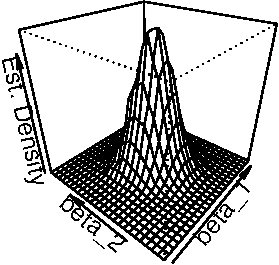
\includegraphics{ITER_files/figure-latex/unnamed-chunk-270-1} \end{center}

From the plot above we can see that the density estimate has some
similarity to a bivariate normal distribution (see Chapter \ref{pt})
though it is not very pretty and probably a little rough. Furthermore,
there is a correlation between the estimates such that \(\rho\neq0\) in
(2.1). Also, the distribution's shape deviates from the symmetric bell
shape of the bivariate standard normal distribution and has an
elliptical surface area instead.

\begin{Shaded}
\begin{Highlighting}[]
\CommentTok{# estimate the correlation between estimators}
\KeywordTok{cor}\NormalTok{(coefs[, }\DecValTok{1}\NormalTok{], coefs[, }\DecValTok{2}\NormalTok{])}
\end{Highlighting}
\end{Shaded}

\begin{verbatim}
## [1] -0.2503028
\end{verbatim}

Where does this correlation come from? Notice that, due to the way we
generated the data, there is correlation between the regressors \(X_1\)
and \(X_2\). Correlation between the regressors in a multiple regression
model always translates into correlation between the estimators (see
Appendix 6.2 of the book). In our case, the positive correlation between
\(X_1\) and \(X_2\) translates to negative correlation between
\(\hat\beta_1\) and \(\hat\beta_2\). To get a better idea of the
distribution you can vary the point of view in the subsequent smooth
interactive 3D plot of the same density estimate used for plotting with
\texttt{persp()}. Here you can see that the shape of the distribution is
somewhat stretched due to \(\rho=-0.20\) and it is also apparent that
both estimators are unbiased since their joint density seems to be
centered close to the true parameter vector
\((\beta_1,\beta_2) = (2.5,3)\).

\begin{center}\textit{This interactive part of the book is only available in the HTML version.}\end{center}

\section{Exercises}\label{exercises-4}

\begin{center}\textit{This interactive part of the book is only available in the HTML version.}\end{center}

\chapter{Hypothesis Tests and Confidence Intervals in Multiple
Regression}\label{htaciimr}

This chapter discusses methods that allow to quantify the sampling
uncertainty in the OLS estimator of the coefficients in multiple
regression models. The basis for this are hypothesis tests and
confidence intervals which, just as for the simple linear regression
model, can be computed using basic \texttt{R} functions. We will also
tackle the issue of testing joint hypotheses on these coefficients.

Make sure the packages \texttt{AER} \citep{R-AER} and \texttt{stargazer}
\citep{R-stargazer} are installed before you go ahead and replicate the
examples. The safest way to do so is by checking whether the following
code chunk executes without any issues.

\begin{Shaded}
\begin{Highlighting}[]
\KeywordTok{library}\NormalTok{(AER)}
\KeywordTok{library}\NormalTok{(stargazer)}
\end{Highlighting}
\end{Shaded}

\section{Hypothesis Tests and Confidence Intervals for a Single
Coefficient}\label{hypothesis-tests-and-confidence-intervals-for-a-single-coefficient}

We first discuss how to compute standard errors, how to test hypotheses
and how to construct confidence intervals for a single regression
coefficient \(\beta_j\) in a multiple regression model. The basic idea
is summarized in Key Concept 7.1.

\begin{keyconcepts}[Testing the Hypothesis $\beta_j = \beta_{j,0}$
                    Against the Alternative $\beta_j \neq \beta_{j,0}$]{7.1}
\begin{enumerate}
\item Compute the standard error of $\hat{\beta_j}$
\item Compute the $t$-statistic,
$$t^{act} = \frac{\hat{\beta}_j - \beta_{j,0}} {SE(\hat{\beta_j})}$$
\item Compute the $p$-value,
$$p\text{-value} = 2 \Phi(-|t^{act}|)$$
where $t^{act}$ is the value of the $t$-statistic actually computed. Reject the hypothesis at the $5\%$ significance level if the $p$-value is less than $0.05$ or, equivalently, if $|t^{act}| > 1.96$. \end{enumerate}\vspace{0.5cm}

The standard error and (typically) the $t$-statistic and the corresponding $p$-value for testing $\beta_j = 0$ are computed automatically by suitable \texttt{R} functions, e.g., by \texttt{summary()}.
\end{keyconcepts}

Testing a single hypothesis about the significance of a coefficient in
the multiple regression model proceeds as in in the simple regression
model.

You can easily see this by inspecting the coefficient summary of the
regression model

\[ TestScore = \beta_0 + \beta_1 \times size  \beta_2 \times english + u \]

already discussed in Chapter \ref{rmwmr}. Let us review this:

\begin{Shaded}
\begin{Highlighting}[]
\NormalTok{model <-}\StringTok{ }\KeywordTok{lm}\NormalTok{(score }\OperatorTok{~}\StringTok{ }\NormalTok{size }\OperatorTok{+}\StringTok{ }\NormalTok{english, }\DataTypeTok{data =}\NormalTok{ CASchools)}
\KeywordTok{coeftest}\NormalTok{(model, }\DataTypeTok{vcov. =}\NormalTok{ vcovHC, }\DataTypeTok{type =} \StringTok{"HC1"}\NormalTok{)}
\end{Highlighting}
\end{Shaded}

\begin{verbatim}
## 
## t test of coefficients:
## 
##               Estimate Std. Error  t value Pr(>|t|)    
## (Intercept) 686.032245   8.728225  78.5993  < 2e-16 ***
## size         -1.101296   0.432847  -2.5443  0.01131 *  
## english      -0.649777   0.031032 -20.9391  < 2e-16 ***
## ---
## Signif. codes:  0 '***' 0.001 '**' 0.01 '*' 0.05 '.' 0.1 ' ' 1
\end{verbatim}

You may check that these quantities are computed as in the simple
regression model by computing the \(t\)-statistics or \(p\)-values by
hand using the output above and \texttt{R} as a calculator.

For example, using the definition of the \(p\)-value for a two-sided
test as given in Key Concept 7.1, we can confirm the \(p\)-value for a
test of the hypothesis that the coefficient \(\beta_1\), the coefficient
on \texttt{size}, to be approximately zero.

\begin{Shaded}
\begin{Highlighting}[]
\CommentTok{# compute two-sided p-value}
\DecValTok{2} \OperatorTok{*}\StringTok{ }\NormalTok{(}\DecValTok{1} \OperatorTok{-}\StringTok{ }\KeywordTok{pt}\NormalTok{(}\KeywordTok{abs}\NormalTok{(}\KeywordTok{coeftest}\NormalTok{(model, }\DataTypeTok{vcov. =}\NormalTok{ vcovHC, }\DataTypeTok{type =} \StringTok{"HC1"}\NormalTok{)[}\DecValTok{2}\NormalTok{, }\DecValTok{3}\NormalTok{]),}
            \DataTypeTok{df =}\NormalTok{ model}\OperatorTok{$}\NormalTok{df.residual))}
\end{Highlighting}
\end{Shaded}

\begin{verbatim}
## [1] 0.01130921
\end{verbatim}

\begin{keyconcepts}[Confidence Intervals for a Single Coefficient in Multiple Regression]{7.2}
A $95\%$ two-sided confidence interval for the coefficient $\beta_j$ is an interval that contains the true value of $\beta_j$ with a $95 \%$ probability; that is, it contains the true value of $\beta_j$ in $95 \%$ of repeated samples. Equivalently, it is the set of values of $\beta_j$ that cannot be rejected by a $5 \%$ two-sided hypothesis test. When the sample size is large, the $95 \%$ confidence interval for $\beta_j$ is
$$\left[\hat{\beta_j}- 1.96 \times SE(\hat{\beta}_j), \hat{\beta_j} + 1.96 \times SE(\hat{\beta_j})\right].$$
\end{keyconcepts}

\section{An Application to Test Scores and the Student-Teacher
Ratio}\label{an-application-to-test-scores-and-the-student-teacher-ratio}

Let us take a look at the regression from Section \ref{mofimr} again.

Computing confidence intervals for individual coefficients in the
multiple regression model proceeds as in the simple regression model
using the function \texttt{confint()}.

\begin{Shaded}
\begin{Highlighting}[]
\NormalTok{model <-}\StringTok{ }\KeywordTok{lm}\NormalTok{(score }\OperatorTok{~}\StringTok{ }\NormalTok{size }\OperatorTok{+}\StringTok{ }\NormalTok{english, }\DataTypeTok{data =}\NormalTok{ CASchools)}
\KeywordTok{confint}\NormalTok{(model)}
\end{Highlighting}
\end{Shaded}

\begin{verbatim}
##                   2.5 %      97.5 %
## (Intercept) 671.4640580 700.6004311
## size         -1.8487969  -0.3537944
## english      -0.7271113  -0.5724424
\end{verbatim}

To obtain confidence intervals at another level, say \(90\%\), just set
the argument \texttt{level} in our call of \texttt{confint()}
accordingly.

\begin{Shaded}
\begin{Highlighting}[]
\KeywordTok{confint}\NormalTok{(model, }\DataTypeTok{level =} \FloatTok{0.9}\NormalTok{)}
\end{Highlighting}
\end{Shaded}

\begin{verbatim}
##                     5 %        95 %
## (Intercept) 673.8145793 698.2499098
## size         -1.7281904  -0.4744009
## english      -0.7146336  -0.5849200
\end{verbatim}

The output now reports the desired \(90\%\) confidence intervals for all
coefficients.

A disadvantage of \texttt{confint()} is that is does not use robust
standard errors to compute the confidence interval. For large-sample
confidence intervals, this is quickly done manually as follows.

\begin{Shaded}
\begin{Highlighting}[]
\CommentTok{# compute robust standard errors}
\NormalTok{rob_se <-}\StringTok{ }\KeywordTok{diag}\NormalTok{(}\KeywordTok{vcovHC}\NormalTok{(model, }\DataTypeTok{type =} \StringTok{"HC1"}\NormalTok{))}\OperatorTok{^}\FloatTok{0.5}

\CommentTok{# compute robust 95% confidence intervals}
\KeywordTok{rbind}\NormalTok{(}\StringTok{"lower"}\NormalTok{ =}\StringTok{ }\KeywordTok{coef}\NormalTok{(model) }\OperatorTok{-}\StringTok{ }\KeywordTok{qnorm}\NormalTok{(}\FloatTok{0.975}\NormalTok{) }\OperatorTok{*}\StringTok{ }\NormalTok{rob_se,}
      \StringTok{"upper"}\NormalTok{ =}\StringTok{ }\KeywordTok{coef}\NormalTok{(model) }\OperatorTok{+}\StringTok{ }\KeywordTok{qnorm}\NormalTok{(}\FloatTok{0.975}\NormalTok{) }\OperatorTok{*}\StringTok{ }\NormalTok{rob_se)}
\end{Highlighting}
\end{Shaded}

\begin{verbatim}
##       (Intercept)       size    english
## lower    668.9252 -1.9496606 -0.7105980
## upper    703.1393 -0.2529307 -0.5889557
\end{verbatim}

\begin{Shaded}
\begin{Highlighting}[]
\CommentTok{# compute robust 90% confidence intervals}

\KeywordTok{rbind}\NormalTok{(}\StringTok{"lower"}\NormalTok{ =}\StringTok{ }\KeywordTok{coef}\NormalTok{(model) }\OperatorTok{-}\StringTok{ }\KeywordTok{qnorm}\NormalTok{(}\FloatTok{0.95}\NormalTok{) }\OperatorTok{*}\StringTok{ }\NormalTok{rob_se,}
      \StringTok{"upper"}\NormalTok{ =}\StringTok{ }\KeywordTok{coef}\NormalTok{(model) }\OperatorTok{+}\StringTok{ }\KeywordTok{qnorm}\NormalTok{(}\FloatTok{0.95}\NormalTok{) }\OperatorTok{*}\StringTok{ }\NormalTok{rob_se)}
\end{Highlighting}
\end{Shaded}

\begin{verbatim}
##       (Intercept)       size    english
## lower    671.6756 -1.8132659 -0.7008195
## upper    700.3889 -0.3893254 -0.5987341
\end{verbatim}

Knowing how to use \texttt{R} to make inference about the coefficients
in multiple regression models, you can now answer the following
question:

Can the null hypothesis that a change in the student-teacher ratio,
\texttt{size}, has no significant influence on test scores,
\texttt{scores}, --- if we control for the percentage of students
learning English in the district, \texttt{english}, --- be rejected at
the \(10\%\) and the \(5\%\) level of significance?

The output above shows that zero is not an element of the confidence
interval for the coefficient on \texttt{size} such that we can reject
the null hypothesis at significance levels of \(5\%\) and \(10\%\). The
same conclusion can be made via the \(p\)-value for \texttt{size}:
\(0.00398 < 0.05 = \alpha\).

Note that rejection at the \(5\%\)-level implies rejection at the
\(10\%\) level (why?).

Recall from Chapter \ref{cifrc} the \(95\%\) confidence interval
computed above \emph{does not} tell us that a one-unit decrease in the
student-teacher ratio has an effect on test scores that lies in the
interval with a lower bound of \(-1.9497\) and an upper bound of
\(-0.2529\). Once a confidence interval has been computed, a
probabilistic statement like this is wrong: either the interval contains
the true parameter or it does not. We do not know which is true.

\subsection*{Another Augmentation of the
Model}\label{another-augmentation-of-the-model}
\addcontentsline{toc}{subsection}{Another Augmentation of the Model}

What is the average effect on test scores of reducing the
student-teacher ratio when the expenditures per pupil and the percentage
of english learning pupils are held constant?

Let us augment our model by an additional regressor that is a measure
for expenditure per pupil. Using \texttt{?CASchools} we find that
\texttt{CASchools} contains the variable \texttt{expenditure}, which
provides expenditure per student.

Our model now is
\[ TestScore = \beta_0 + \beta_1 \times size + \beta_2 \times english + \beta_3 \times expenditure + u \]

with \(expenditure\) the total amount of expenditure per pupil in the
district (thousands of dollars).

Let us now estimate the model:

\begin{Shaded}
\begin{Highlighting}[]
\CommentTok{# scale expenditure to thousands of dollars}
\NormalTok{CASchools}\OperatorTok{$}\NormalTok{expenditure <-}\StringTok{ }\NormalTok{CASchools}\OperatorTok{$}\NormalTok{expenditure}\OperatorTok{/}\DecValTok{1000}

\CommentTok{# estimate the model}
\NormalTok{model <-}\StringTok{ }\KeywordTok{lm}\NormalTok{(score }\OperatorTok{~}\StringTok{ }\NormalTok{size }\OperatorTok{+}\StringTok{ }\NormalTok{english }\OperatorTok{+}\StringTok{ }\NormalTok{expenditure, }\DataTypeTok{data =}\NormalTok{ CASchools)}
\KeywordTok{coeftest}\NormalTok{(model, }\DataTypeTok{vcov. =}\NormalTok{ vcovHC, }\DataTypeTok{type =} \StringTok{"HC1"}\NormalTok{)}
\end{Highlighting}
\end{Shaded}

\begin{verbatim}
## 
## t test of coefficients:
## 
##               Estimate Std. Error  t value Pr(>|t|)    
## (Intercept) 649.577947  15.458344  42.0212  < 2e-16 ***
## size         -0.286399   0.482073  -0.5941  0.55277    
## english      -0.656023   0.031784 -20.6398  < 2e-16 ***
## expenditure   3.867901   1.580722   2.4469  0.01482 *  
## ---
## Signif. codes:  0 '***' 0.001 '**' 0.01 '*' 0.05 '.' 0.1 ' ' 1
\end{verbatim}

The estimated effect of a one unit change in the student-teacher ratio
on test scores with expenditure and the share of english learning pupils
held constant is \(-0.29\), which is rather small. What is more, the
coefficient on \(size\) is not significantly different from zero anymore
even at \(10\%\) since \(p\text{-value}=0.55\). Can you come up with an
interpretation for these findings (see Chapter 7.1 of the book)? The
insignificance of \(\hat\beta_1\) could be due to a larger standard
error of \(\hat{\beta}_1\) resulting from adding \(expenditure\) to the
model so that we estimate the coefficient on \(size\) less precisely.
This illustrates the issue of strongly correlated regressors (imperfect
multicollinearity). The correlation between \(size\) and \(expenditure\)
can be computed using \texttt{cor()}.

\begin{Shaded}
\begin{Highlighting}[]
\CommentTok{# compute the sample correlation between 'size' and 'expenditure'}
\KeywordTok{cor}\NormalTok{(CASchools}\OperatorTok{$}\NormalTok{size, CASchools}\OperatorTok{$}\NormalTok{expenditure)}
\end{Highlighting}
\end{Shaded}

\begin{verbatim}
## [1] -0.6199822
\end{verbatim}

Altogether, we conclude that the new model provides no evidence that
changing the student-teacher ratio, e.g., by hiring new teachers, has
any effect on the test scores while keeping expenditures per student and
the share of English learners constant.

\section{Joint Hypothesis Testing Using the
F-Statistic}\label{joint-hypothesis-testing-using-the-f-statistic}

The estimated model is

\[ \widehat{TestScore} = \underset{(15.21)}{649.58} -\underset{(0.48)}{0.29} \times size - \underset{(0.04)}{0.66} \times english + \underset{(1.41)}{3.87} \times expenditure. \]

Now, can we reject the hypothesis that the coefficient on \(size\)
\emph{and} the coefficient on \(expenditure\) are zero? To answer this,
we have to resort to joint hypothesis tests. A joint hypothesis imposes
restrictions on multiple regression coefficients. This is different from
conducting individual \(t\)-tests where a restriction is imposed on a
single coefficient. Chapter 7.2 of the book explains why testing
hypotheses about the model coefficients one at a time is different from
testing them jointly.

The homoskedasticity-only \(F\)-Statistic is given by

\[ F = \frac{(SSR_{\text{restricted}} - SSR_{\text{unrestricted}})/q}{SSR_{\text{unrestricted}} / (n-k-1)} \]

with \(SSR_{restricted}\) being the sum of squared residuals from the
restricted regression, i.e., the regression where we impose the
restriction. \(SSR_{unrestricted}\) is the sum of squared residuals from
the full model, \(q\) is the number of restrictions under the null and
\(k\) is the number of regressors in the unrestricted regression.

It is fairly easy to conduct \(F\)-tests in \texttt{R}. We can use the
function \texttt{linearHypothesis()}contained in the package
\texttt{car}.

\begin{Shaded}
\begin{Highlighting}[]
\CommentTok{# estimate the multiple regression model}
\NormalTok{model <-}\StringTok{ }\KeywordTok{lm}\NormalTok{(score }\OperatorTok{~}\StringTok{ }\NormalTok{size }\OperatorTok{+}\StringTok{ }\NormalTok{english }\OperatorTok{+}\StringTok{ }\NormalTok{expenditure, }\DataTypeTok{data =}\NormalTok{ CASchools)}

\CommentTok{# execute the function on the model object and provide both linear restrictions }
\CommentTok{# to be tested as strings}
\KeywordTok{linearHypothesis}\NormalTok{(model, }\KeywordTok{c}\NormalTok{(}\StringTok{"size=0"}\NormalTok{, }\StringTok{"expenditure=0"}\NormalTok{))}
\end{Highlighting}
\end{Shaded}

\begin{verbatim}
## Linear hypothesis test
## 
## Hypothesis:
## size = 0
## expenditure = 0
## 
## Model 1: restricted model
## Model 2: score ~ size + english + expenditure
## 
##   Res.Df   RSS Df Sum of Sq      F   Pr(>F)    
## 1    418 89000                                 
## 2    416 85700  2    3300.3 8.0101 0.000386 ***
## ---
## Signif. codes:  0 '***' 0.001 '**' 0.01 '*' 0.05 '.' 0.1 ' ' 1
\end{verbatim}

The output reveals that the \(F\)-statistic for this joint hypothesis
test is about \(8.01\) and the corresponding \(p\)-value is \(0.0004\).
Thus, we can reject the null hypothesis that both coefficients are zero
at any level of significance commonly used in practice.

A heteroskedasticity-robust version of this \(F\)-test (which leads to
the same conclusion) can be conducted as follows.

\begin{Shaded}
\begin{Highlighting}[]
\CommentTok{# heteroskedasticity-robust F-test}
\KeywordTok{linearHypothesis}\NormalTok{(model, }\KeywordTok{c}\NormalTok{(}\StringTok{"size=0"}\NormalTok{, }\StringTok{"expenditure=0"}\NormalTok{), }\DataTypeTok{white.adjust =} \StringTok{"hc1"}\NormalTok{)}
\end{Highlighting}
\end{Shaded}

\begin{verbatim}
## Linear hypothesis test
## 
## Hypothesis:
## size = 0
## expenditure = 0
## 
## Model 1: restricted model
## Model 2: score ~ size + english + expenditure
## 
## Note: Coefficient covariance matrix supplied.
## 
##   Res.Df Df      F   Pr(>F)   
## 1    418                      
## 2    416  2 5.4337 0.004682 **
## ---
## Signif. codes:  0 '***' 0.001 '**' 0.01 '*' 0.05 '.' 0.1 ' ' 1
\end{verbatim}

The standard output of a model summary also reports an \(F\)-statistic
and the corresponding \(p\)-value. The null hypothesis belonging to this
\(F\)-test is that \emph{all} of the population coefficients in the
model except for the intercept are zero, so the hypotheses are
\[H_0: \beta_1=0, \ \beta_2 =0, \ \beta_3 =0 \quad \text{vs.} \quad H_1: \beta_j \neq 0 \ \text{for at least one} \ j=1,2,3.\]

This is also called the \emph{overall regression \(F\)-statistic} and
the null hypothesis is obviously different from testing if only
\(\beta_1\) and \(\beta_3\) are zero.

We now check whether the \(F\)-statistic belonging to the \(p\)-value
listed in the model's summary coincides with the result reported by
\texttt{linearHypothesis()}.

\begin{Shaded}
\begin{Highlighting}[]
\CommentTok{# execute the function on the model object and provide the restrictions }
\CommentTok{# to be tested as a character vector}
\KeywordTok{linearHypothesis}\NormalTok{(model, }\KeywordTok{c}\NormalTok{(}\StringTok{"size=0"}\NormalTok{, }\StringTok{"english=0"}\NormalTok{, }\StringTok{"expenditure=0"}\NormalTok{))}
\end{Highlighting}
\end{Shaded}

\begin{verbatim}
## Linear hypothesis test
## 
## Hypothesis:
## size = 0
## english = 0
## expenditure = 0
## 
## Model 1: restricted model
## Model 2: score ~ size + english + expenditure
## 
##   Res.Df    RSS Df Sum of Sq      F    Pr(>F)    
## 1    419 152110                                  
## 2    416  85700  3     66410 107.45 < 2.2e-16 ***
## ---
## Signif. codes:  0 '***' 0.001 '**' 0.01 '*' 0.05 '.' 0.1 ' ' 1
\end{verbatim}

\begin{Shaded}
\begin{Highlighting}[]
\CommentTok{# Access the overall F-statistic from the model's summary}
\KeywordTok{summary}\NormalTok{(model)}\OperatorTok{$}\NormalTok{fstatistic}
\end{Highlighting}
\end{Shaded}

\begin{verbatim}
##    value    numdf    dendf 
## 107.4547   3.0000 416.0000
\end{verbatim}

The entry \texttt{value} is the overall \(F\)-statistics and it equals
the result of \texttt{linearHypothesis()}. The \(F\)-test rejects the
null hypothesis that the model has no power in explaining test scores.
It is important to know that the \(F\)-statistic reported by
\texttt{summary} is \emph{not} robust to heteroskedasticity!

\section{Confidence Sets for Multiple
Coefficients}\label{confidence-sets-for-multiple-coefficients}

Based on the \(F\)-statistic that we have previously encountered, we can
specify confidence sets. Confidence sets are analogous to confidence
intervals for single coefficients. As such, confidence sets consist of
\emph{combinations} of coefficients that contain the true combination of
coefficients in, say, \(95\%\) of all cases if we could repeatedly draw
random samples, just like in the univariate case. Put differently, a
confidence set is the set of all coefficient combinations for which we
cannot reject the corresponding joint null hypothesis tested using an
\(F\)-test.

The confidence set for two coefficients an ellipse which is centered
around the point defined by both coefficient estimates. Again, there is
a very convenient way to plot the confidence set for two coefficients of
model objects, namely the function \texttt{confidenceEllipse()} from the
\texttt{car} package.

We now plot the \(95\%\) confidence ellipse for the coefficients on
\texttt{size} and \texttt{expenditure} from the regression conducted
above. By specifying the additional argument \texttt{fill}, the
confidence set is colored.

\begin{Shaded}
\begin{Highlighting}[]
\CommentTok{# draw the 95% confidence set for coefficients on size and expenditure}
\KeywordTok{confidenceEllipse}\NormalTok{(model, }
                  \DataTypeTok{fill =}\NormalTok{ T,}
                  \DataTypeTok{lwd =} \DecValTok{0}\NormalTok{,}
                  \DataTypeTok{which.coef =} \KeywordTok{c}\NormalTok{(}\StringTok{"size"}\NormalTok{, }\StringTok{"expenditure"}\NormalTok{),}
                  \DataTypeTok{main =} \StringTok{"95% Confidence Set"}\NormalTok{)}
\end{Highlighting}
\end{Shaded}

\begin{center}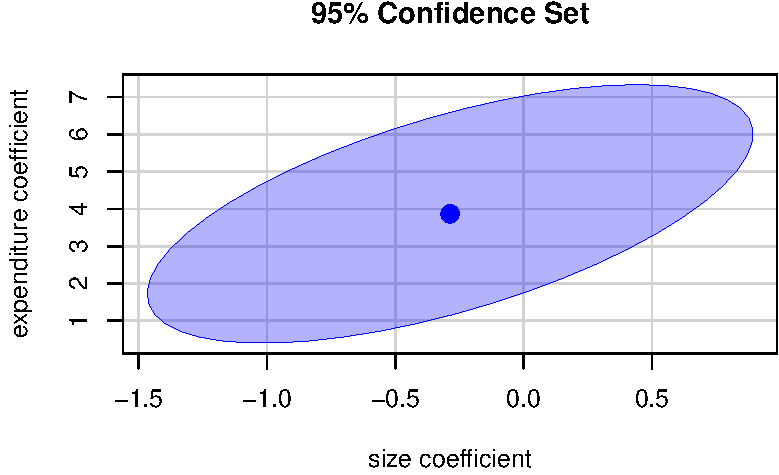
\includegraphics{ITER_files/figure-latex/unnamed-chunk-294-1} \end{center}

We see that the ellipse is centered around \((-0.29, 3.87)\), the pair
of coefficients estimates on \(size\) and \(expenditure\). What is more,
\((0,0)\) is not element of the \(95\%\) confidence set so that we can
reject \(H_0: \beta_1 = 0, \ \beta_3 = 0\).

By default, \texttt{confidenceEllipse()} uses homoskedasticity-only
standard errors. The following code chunk shows how compute a robust
confidence ellipse and how to overlay it with the previous plot.

\begin{Shaded}
\begin{Highlighting}[]
\CommentTok{# draw the robust 95% confidence set for coefficients on size and expenditure }
\KeywordTok{confidenceEllipse}\NormalTok{(model, }
                  \DataTypeTok{fill =}\NormalTok{ T,}
                  \DataTypeTok{lwd =} \DecValTok{0}\NormalTok{,}
                  \DataTypeTok{which.coef =} \KeywordTok{c}\NormalTok{(}\StringTok{"size"}\NormalTok{, }\StringTok{"expenditure"}\NormalTok{),}
                  \DataTypeTok{main =} \StringTok{"95% Confidence Sets"}\NormalTok{,}
                  \DataTypeTok{vcov. =} \KeywordTok{vcovHC}\NormalTok{(model, }\DataTypeTok{type =} \StringTok{"HC1"}\NormalTok{),}
                  \DataTypeTok{col =} \StringTok{"red"}\NormalTok{)}
                  
\CommentTok{# draw the 95% confidence set for coefficients on size and expenditure}
\KeywordTok{confidenceEllipse}\NormalTok{(model, }
                  \DataTypeTok{fill =}\NormalTok{ T,}
                  \DataTypeTok{lwd =} \DecValTok{0}\NormalTok{,}
                  \DataTypeTok{which.coef =} \KeywordTok{c}\NormalTok{(}\StringTok{"size"}\NormalTok{, }\StringTok{"expenditure"}\NormalTok{),}
                  \DataTypeTok{add =}\NormalTok{ T)}
\end{Highlighting}
\end{Shaded}

\begin{center}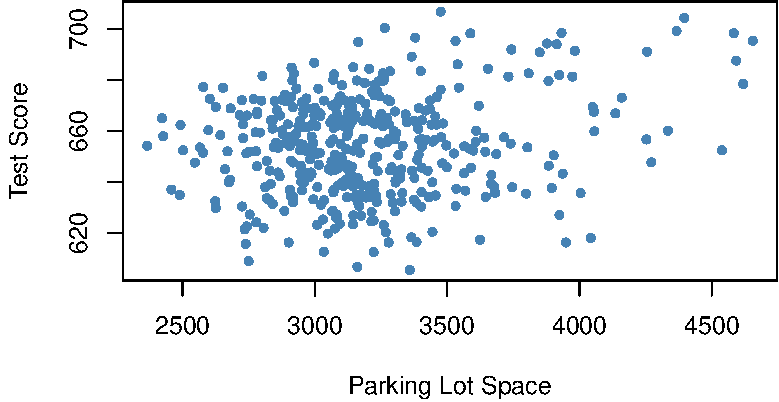
\includegraphics{ITER_files/figure-latex/unnamed-chunk-295-1} \end{center}

As the robust standard errors are slightly larger than those valid under
homoskedasticity only in this case, the robust confidence set is
slightly larger. This is analogous to the confidence intervals for the
individual coefficients.

\section{Model Specification for Multiple
Regression}\label{model-specification-for-multiple-regression}

Choosing a regression specification, i.e., selecting the variables to be
included in a regression model, is a difficult task. However, there are
some guidelines on how to proceed. The goal is clear: obtaining an
unbiased and precise estimate of the causal effect of interest. As a
starting point, think about omitted variables, that is, to avoid
possible bias by using suitable control variables. Omitted variables
bias in the context of multiple regression is explained in Key Concept
7.3. A second step could be to compare different specifications by
measures of fit. However, as we shall see one should not rely solely on
\(\bar{R}^2\).

\begin{keyconcepts}[Omitted Variable Bias in Multiple Regression]{7.3}
Omitted variable bias is the bias in the OLS estimator that arises when regressors correlate with an omitted variable. For omitted variable bias to arise, two things must be true:\newline

\begin{enumerate}
\item At least one of the included regressors must be correlated with the omitted variable. 
\item The omitted variable must be a determinant of the dependent variable, $Y$.
\end{enumerate}

\end{keyconcepts}

We now discuss an example were we face a potential omitted variable bias
in a multiple regression model:

Consider again the estimated regression equation

\[ \widehat{TestScore} = \underset{(8.7)}{686.0} - \underset{(0.43)}{1.10} \times size - \underset{(0.031)}{0.650} \times english. \]

We are interested in estimating the causal effect of class size on test
score. There might be a bias due to omitting ``outside learning
opportunities'' from our regression since such a measure could be a
determinant of the students' test scores and could also be correlated
with both regressors already included in the model (so that both
conditions of Key Concept 7.3 are fulfilled). ``Outside learning
opportunities'' are a complicated concept that is difficult to quantify.
A surrogate we can consider instead is the students' economic background
which likely are strongly related to outside learning opportunities:
think of wealthy parents that are able to provide time and/or money for
private tuition of their children. We thus augment the model with the
variable \texttt{lunch}, the percentage of students that qualify for a
free or subsidized lunch in school due to family incomes below a certain
threshold, and reestimate the model.

\begin{Shaded}
\begin{Highlighting}[]
\CommentTok{# estimate the model and print the summary to console}
\NormalTok{model <-}\StringTok{ }\KeywordTok{lm}\NormalTok{(score }\OperatorTok{~}\StringTok{ }\NormalTok{size }\OperatorTok{+}\StringTok{ }\NormalTok{english }\OperatorTok{+}\StringTok{ }\NormalTok{lunch, }\DataTypeTok{data =}\NormalTok{ CASchools)}
\KeywordTok{coeftest}\NormalTok{(model, }\DataTypeTok{vcov. =}\NormalTok{ vcovHC, }\DataTypeTok{type =} \StringTok{"HC1"}\NormalTok{)}
\end{Highlighting}
\end{Shaded}

\begin{verbatim}
## 
## t test of coefficients:
## 
##               Estimate Std. Error  t value  Pr(>|t|)    
## (Intercept) 700.149957   5.568453 125.7351 < 2.2e-16 ***
## size         -0.998309   0.270080  -3.6963 0.0002480 ***
## english      -0.121573   0.032832  -3.7029 0.0002418 ***
## lunch        -0.547345   0.024107 -22.7046 < 2.2e-16 ***
## ---
## Signif. codes:  0 '***' 0.001 '**' 0.01 '*' 0.05 '.' 0.1 ' ' 1
\end{verbatim}

Thus, the estimated regression line is

\[ \widehat{TestScore} = \underset{(5.56)}{700.15} - \underset{(0.27)}{1.00} \times size - \underset{(0.03)}{0.12} \times english - \underset{(0.02)}{0.55} \times lunch. \]

We observe no substantial changes in the conclusion about the effect of
\(size\) on \(TestScore\): the coefficient on \(size\) changes by only
\(0.1\) and retains its significance.

Although the difference in estimated coefficients is not big in this
case, it is useful to keep \texttt{lunch} to make the assumption of
conditional mean independence more credible (see Chapter 7.5 of the
book).

\subsection*{Model Specification in Theory and in
Practice}\label{model-specification-in-theory-and-in-practice}
\addcontentsline{toc}{subsection}{Model Specification in Theory and in
Practice}

Key Concept 7.4 lists some common pitfalls when using \(R^2\) and
\(\bar{R}^2\) to evaluate the predictive ability of regression models.

\begin{keyconcepts}[$R^2$ and $\bar{R}^2$: What They Tell You --- and What They Do not]{7.4}
The $R^2$ and $\bar{R}^2$ tell you whether the regressors are good at explaining the variation of the independent variable in the sample. If the $R^2$ (or $\bar{R}^2$) is nearly $1$, then the regressors produce a good prediction of the dependent variable in that sample, in the sense that the variance of OLS residuals is small compared to the variance of the dependent variable. If the $R^2$ (or $\bar{R}^2$) is nearly $0$, the opposite is true.\newline

The $R^2$ and $\bar{R}^2$ do \textit{not} tell you whether:\newline

\begin{enumerate}
\item An included variable is statistically significant. 
\item The regressors are the true cause of the movements in the dependent variable.
\item There is omitted variable bias.
\item You have chosen the most appropriate set of regressors.
\end{enumerate}
\end{keyconcepts}

For example, think of regressing \(TestScore\) on \(PLS\) which measures
the available parking lot space in thousand square feet. You are likely
to observe a significant coefficient of reasonable magnitude and
moderate to high values for \(R^2\) and \(\bar{R}^2\). The reason for
this is that parking lot space is correlated with many determinants of
the test score like location, class size, financial endowment and so on.
Although we do not have observations on \(PLS\), we can use \texttt{R}
to generate some relatively realistic data.

\begin{Shaded}
\begin{Highlighting}[]
\CommentTok{# set seed for reproducibility}
\KeywordTok{set.seed}\NormalTok{(}\DecValTok{1}\NormalTok{)}

\CommentTok{# generate observations for parking lot space}
\NormalTok{CASchools}\OperatorTok{$}\NormalTok{PLS <-}\StringTok{ }\KeywordTok{c}\NormalTok{(}\DecValTok{22} \OperatorTok{*}\StringTok{ }\NormalTok{CASchools}\OperatorTok{$}\NormalTok{income }
                   \OperatorTok{-}\StringTok{ }\DecValTok{15} \OperatorTok{*}\StringTok{ }\NormalTok{CASchools}\OperatorTok{$}\NormalTok{size }
                   \OperatorTok{+}\StringTok{ }\FloatTok{0.2} \OperatorTok{*}\StringTok{ }\NormalTok{CASchools}\OperatorTok{$}\NormalTok{expenditure}
                   \OperatorTok{+}\StringTok{ }\KeywordTok{rnorm}\NormalTok{(}\KeywordTok{nrow}\NormalTok{(CASchools), }\DataTypeTok{sd =} \DecValTok{80}\NormalTok{) }\OperatorTok{+}\StringTok{ }\DecValTok{3000}\NormalTok{)}
\end{Highlighting}
\end{Shaded}

\begin{Shaded}
\begin{Highlighting}[]
\CommentTok{# plot parking lot space against test score}
\KeywordTok{plot}\NormalTok{(CASchools}\OperatorTok{$}\NormalTok{PLS, }
\NormalTok{     CASchools}\OperatorTok{$}\NormalTok{score,}
     \DataTypeTok{xlab =} \StringTok{"Parking Lot Space"}\NormalTok{,}
     \DataTypeTok{ylab =} \StringTok{"Test Score"}\NormalTok{,}
     \DataTypeTok{pch =} \DecValTok{20}\NormalTok{,}
     \DataTypeTok{col =} \StringTok{"steelblue"}\NormalTok{)}
\end{Highlighting}
\end{Shaded}

\begin{center}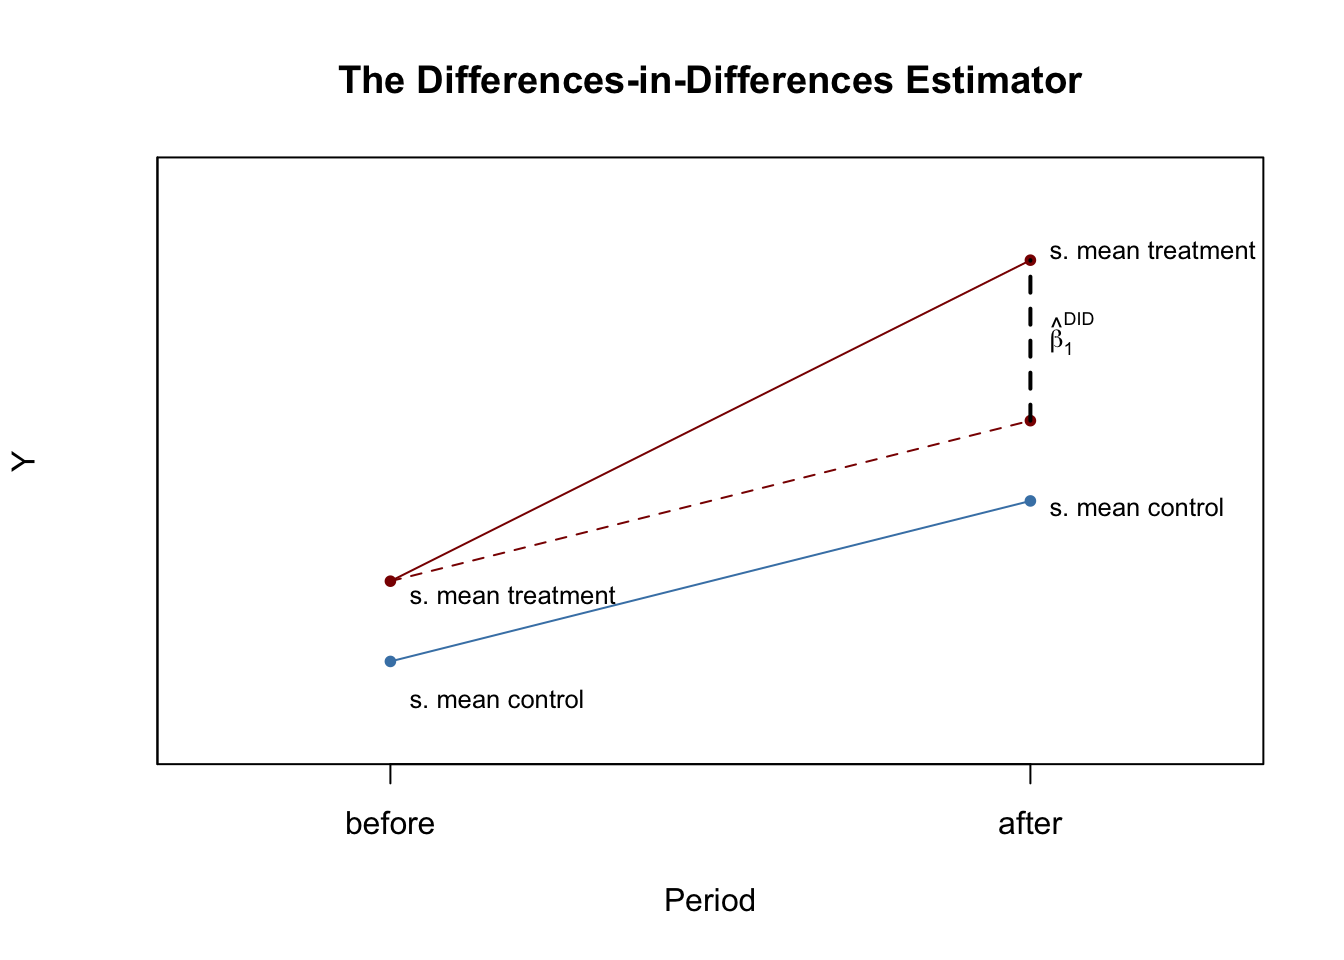
\includegraphics{ITER_files/figure-latex/unnamed-chunk-302-1} \end{center}

\begin{Shaded}
\begin{Highlighting}[]
\CommentTok{# regress test score on PLS}
\KeywordTok{summary}\NormalTok{(}\KeywordTok{lm}\NormalTok{(score }\OperatorTok{~}\StringTok{ }\NormalTok{PLS, }\DataTypeTok{data =}\NormalTok{ CASchools))}
\end{Highlighting}
\end{Shaded}

\begin{verbatim}
## 
## Call:
## lm(formula = score ~ PLS, data = CASchools)
## 
## Residuals:
##     Min      1Q  Median      3Q     Max 
## -42.608 -11.049   0.342  12.558  37.105 
## 
## Coefficients:
##              Estimate Std. Error t value Pr(>|t|)    
## (Intercept) 4.897e+02  1.227e+01   39.90   <2e-16 ***
## PLS         4.002e-02  2.981e-03   13.43   <2e-16 ***
## ---
## Signif. codes:  0 '***' 0.001 '**' 0.01 '*' 0.05 '.' 0.1 ' ' 1
## 
## Residual standard error: 15.95 on 418 degrees of freedom
## Multiple R-squared:  0.3013, Adjusted R-squared:  0.2996 
## F-statistic: 180.2 on 1 and 418 DF,  p-value: < 2.2e-16
\end{verbatim}

\(PLS\) is generated as a linear function of \(expenditure\),
\(income\), \(size\) and a random disturbance. Therefore the data
suggest that there is some positive relationship between parking lot
space and test score. In fact, when estimating the model

\begin{align}
TestScore = \beta_0 + \beta_1 \times PLS + u \label{eq:plsmod} 
\end{align}

using \texttt{lm()} we find that the coefficient on \(PLS\) is positive
and significantly different from zero. Also \(R^2\) and \(\bar{R}^2\)
are about \(0.3\) which is a lot more than the roughly \(0.05\) observed
when regressing the test scores on the class sizes only. This suggests
that increasing the parking lot space boosts a school's test scores and
that model \eqref{eq:plsmod} does even better in explaining heterogeneity
in the dependent variable than a model with \(size\) as the only
regressor. Keeping in mind how \(PLS\) is constructed this comes as no
surprise. It is evident that the high \(R^2\) cannot be used to the
conclude that the estimated relation between parking lot space and test
scores is causal: the (relatively) high \(R^2\) is due to correlation
between \(PLS\) and other determinants and/or control variables.
Increasing parking lot space is \emph{not} an appropriate measure to
generate more learning success!

\section{Analysis of the Test Score Data
Set}\label{analysis-of-the-test-score-data-set}

Chapter \ref{rmwmr} and some of the previous sections have stressed that
it is important to include control variables in regression models if it
is plausible that there are omitted factors. In our example of test
scores we want to estimate the causal effect of a change in the
student-teacher ratio on test scores. We now provide an example how to
use multiple regression in order to alleviate omitted variable bias and
demonstrate how to report results using \texttt{R}.

So far we have considered two variables that control for unobservable
student characteristics which correlate with the student-teacher ratio
\emph{and} are assumed to have an impact on test scores:

\begin{itemize}
\item
  \(English\), the percentage of English learning students
\item
  \(lunch\), the share of students that qualify for a subsidized or even
  a free lunch at school
\end{itemize}

Another new variable provided with \texttt{CASchools} is
\texttt{calworks}, the percentage of students that qualify for the
\emph{CalWorks} income assistance program. Students eligible for
\emph{CalWorks} live in families with a total income below the threshold
for the subsidized lunch program so both variables are indicators for
the share of economically disadvantaged children. Both indicators are
highly correlated:

\begin{Shaded}
\begin{Highlighting}[]
\CommentTok{# estimate the correlation between 'calworks' and 'lunch'}
\KeywordTok{cor}\NormalTok{(CASchools}\OperatorTok{$}\NormalTok{calworks, CASchools}\OperatorTok{$}\NormalTok{lunch)}
\end{Highlighting}
\end{Shaded}

\begin{verbatim}
## [1] 0.7394218
\end{verbatim}

There is no unambiguous way to proceed when deciding which variable to
use. In any case it may not a good idea to use both variables as
regressors in view of collinearity. Therefore, we also consider
alternative model specifications.

For a start, we plot student characteristics against test scores.

\begin{Shaded}
\begin{Highlighting}[]
\CommentTok{# set up arrangement of plots}
\NormalTok{m <-}\StringTok{ }\KeywordTok{rbind}\NormalTok{(}\KeywordTok{c}\NormalTok{(}\DecValTok{1}\NormalTok{, }\DecValTok{2}\NormalTok{), }\KeywordTok{c}\NormalTok{(}\DecValTok{3}\NormalTok{, }\DecValTok{0}\NormalTok{))}
\NormalTok{graphics}\OperatorTok{::}\KeywordTok{layout}\NormalTok{(}\DataTypeTok{mat =}\NormalTok{ m)}

\CommentTok{# scatterplots}
\KeywordTok{plot}\NormalTok{(score }\OperatorTok{~}\StringTok{ }\NormalTok{english, }
     \DataTypeTok{data =}\NormalTok{ CASchools, }
     \DataTypeTok{col =} \StringTok{"steelblue"}\NormalTok{, }
     \DataTypeTok{pch =} \DecValTok{20}\NormalTok{, }
     \DataTypeTok{xlim =} \KeywordTok{c}\NormalTok{(}\DecValTok{0}\NormalTok{, }\DecValTok{100}\NormalTok{),}
     \DataTypeTok{cex.main =} \FloatTok{0.9}\NormalTok{,}
     \DataTypeTok{main =} \StringTok{"Percentage of English language learners"}\NormalTok{)}

\KeywordTok{plot}\NormalTok{(score }\OperatorTok{~}\StringTok{ }\NormalTok{lunch, }
     \DataTypeTok{data =}\NormalTok{ CASchools, }
     \DataTypeTok{col =} \StringTok{"steelblue"}\NormalTok{, }
     \DataTypeTok{pch =} \DecValTok{20}\NormalTok{,}
     \DataTypeTok{cex.main =} \FloatTok{0.9}\NormalTok{,}
     \DataTypeTok{main =} \StringTok{"Percentage qualifying for reduced price lunch"}\NormalTok{)}

\KeywordTok{plot}\NormalTok{(score }\OperatorTok{~}\StringTok{ }\NormalTok{calworks, }
     \DataTypeTok{data =}\NormalTok{ CASchools, }
     \DataTypeTok{col =} \StringTok{"steelblue"}\NormalTok{, }
     \DataTypeTok{pch =} \DecValTok{20}\NormalTok{, }
     \DataTypeTok{xlim =} \KeywordTok{c}\NormalTok{(}\DecValTok{0}\NormalTok{, }\DecValTok{100}\NormalTok{),}
     \DataTypeTok{cex.main =} \FloatTok{0.9}\NormalTok{,}
     \DataTypeTok{main =} \StringTok{"Percentage qualifying for income assistance"}\NormalTok{)}
\end{Highlighting}
\end{Shaded}

\begin{center}\includegraphics{ITER_files/figure-latex/unnamed-chunk-304-1} \end{center}

We divide the plotting area up using \texttt{layout()}. The matrix
\texttt{m} specifies the location of the plots, see \texttt{?layout}.

We see that all relationships are negative. Here are the correlation
coefficients.

\begin{Shaded}
\begin{Highlighting}[]
\CommentTok{# estimate correlation between student characteristics and test scores}
\KeywordTok{cor}\NormalTok{(CASchools}\OperatorTok{$}\NormalTok{score, CASchools}\OperatorTok{$}\NormalTok{english)}
\end{Highlighting}
\end{Shaded}

\begin{verbatim}
## [1] -0.6441238
\end{verbatim}

\begin{Shaded}
\begin{Highlighting}[]
\KeywordTok{cor}\NormalTok{(CASchools}\OperatorTok{$}\NormalTok{score, CASchools}\OperatorTok{$}\NormalTok{lunch)}
\end{Highlighting}
\end{Shaded}

\begin{verbatim}
## [1] -0.868772
\end{verbatim}

\begin{Shaded}
\begin{Highlighting}[]
\KeywordTok{cor}\NormalTok{(CASchools}\OperatorTok{$}\NormalTok{score, CASchools}\OperatorTok{$}\NormalTok{calworks)}
\end{Highlighting}
\end{Shaded}

\begin{verbatim}
## [1] -0.6268533
\end{verbatim}

We shall consider five different model equations:

\begin{align*}
  (I) \quad TestScore=& \, \beta_0 + \beta_1 \times size + u, \\
  (II) \quad TestScore=& \, \beta_0 + \beta_1 \times size + \beta_2 \times english + u, \\
  (III) \quad TestScore=& \, \beta_0 + \beta_1 \times size + \beta_2 \times english + \beta_3 \times lunch + u, \\
  (IV) \quad TestScore=& \, \beta_0 + \beta_1 \times size + \beta_2 \times english + \beta_4 \times calworks + u, \\
  (V) \quad TestScore=& \, \beta_0 + \beta_1 \times size + \beta_2 \times english + \beta_3 \times lunch + \beta_4 \times calworks + u
\end{align*}

The best way to communicate regression results is in a table. The
\texttt{stargazer} package is very convenient for this purpose. It
provides a function that generates professionally looking HTML and LaTeX
tables that satisfy scientific standards. One simply has to provide one
or multiple object(s) of class \texttt{lm}. The rest is done by the
function \texttt{stargazer()}.

\begin{Shaded}
\begin{Highlighting}[]
\CommentTok{# load the stargazer library}
\KeywordTok{library}\NormalTok{(stargazer)}

\CommentTok{# estimate different model specifications}
\NormalTok{spec1 <-}\StringTok{ }\KeywordTok{lm}\NormalTok{(score }\OperatorTok{~}\StringTok{ }\NormalTok{size, }\DataTypeTok{data =}\NormalTok{ CASchools)}
\NormalTok{spec2 <-}\StringTok{ }\KeywordTok{lm}\NormalTok{(score }\OperatorTok{~}\StringTok{ }\NormalTok{size }\OperatorTok{+}\StringTok{ }\NormalTok{english, }\DataTypeTok{data =}\NormalTok{ CASchools)}
\NormalTok{spec3 <-}\StringTok{ }\KeywordTok{lm}\NormalTok{(score }\OperatorTok{~}\StringTok{ }\NormalTok{size }\OperatorTok{+}\StringTok{ }\NormalTok{english }\OperatorTok{+}\StringTok{ }\NormalTok{lunch, }\DataTypeTok{data =}\NormalTok{ CASchools)}
\NormalTok{spec4 <-}\StringTok{ }\KeywordTok{lm}\NormalTok{(score }\OperatorTok{~}\StringTok{ }\NormalTok{size }\OperatorTok{+}\StringTok{ }\NormalTok{english }\OperatorTok{+}\StringTok{ }\NormalTok{calworks, }\DataTypeTok{data =}\NormalTok{ CASchools)}
\NormalTok{spec5 <-}\StringTok{ }\KeywordTok{lm}\NormalTok{(score }\OperatorTok{~}\StringTok{ }\NormalTok{size }\OperatorTok{+}\StringTok{ }\NormalTok{english }\OperatorTok{+}\StringTok{ }\NormalTok{lunch }\OperatorTok{+}\StringTok{ }\NormalTok{calworks, }\DataTypeTok{data =}\NormalTok{ CASchools)}

\CommentTok{# gather robust standard errors in a list}
\NormalTok{rob_se <-}\StringTok{ }\KeywordTok{list}\NormalTok{(}\KeywordTok{sqrt}\NormalTok{(}\KeywordTok{diag}\NormalTok{(}\KeywordTok{vcovHC}\NormalTok{(spec1, }\DataTypeTok{type =} \StringTok{"HC1"}\NormalTok{))),}
               \KeywordTok{sqrt}\NormalTok{(}\KeywordTok{diag}\NormalTok{(}\KeywordTok{vcovHC}\NormalTok{(spec2, }\DataTypeTok{type =} \StringTok{"HC1"}\NormalTok{))),}
               \KeywordTok{sqrt}\NormalTok{(}\KeywordTok{diag}\NormalTok{(}\KeywordTok{vcovHC}\NormalTok{(spec3, }\DataTypeTok{type =} \StringTok{"HC1"}\NormalTok{))),}
               \KeywordTok{sqrt}\NormalTok{(}\KeywordTok{diag}\NormalTok{(}\KeywordTok{vcovHC}\NormalTok{(spec4, }\DataTypeTok{type =} \StringTok{"HC1"}\NormalTok{))),}
               \KeywordTok{sqrt}\NormalTok{(}\KeywordTok{diag}\NormalTok{(}\KeywordTok{vcovHC}\NormalTok{(spec5, }\DataTypeTok{type =} \StringTok{"HC1"}\NormalTok{))))}

\CommentTok{# generate a LaTeX table using stargazer}
\KeywordTok{stargazer}\NormalTok{(spec1, spec2, spec3, spec4, spec5,}
          \DataTypeTok{se =}\NormalTok{ rob_se,}
          \DataTypeTok{digits =} \DecValTok{3}\NormalTok{,}
          \DataTypeTok{header =}\NormalTok{ F,}
          \DataTypeTok{column.labels =} \KeywordTok{c}\NormalTok{(}\StringTok{"(I)"}\NormalTok{, }\StringTok{"(II)"}\NormalTok{, }\StringTok{"(III)"}\NormalTok{, }\StringTok{"(IV)"}\NormalTok{, }\StringTok{"(V)"}\NormalTok{))}
\end{Highlighting}
\end{Shaded}

\begin{sidewaystable}[!htbp] \centering 
  \caption{\label{tab:rotsostracv} Regressions of Test Scores on the Student-Teacher Ratio and Control Variables} 
  \label{} 
\begin{tabular}{@{\extracolsep{-10pt}}lccccc} 
\\[-1.8ex]\hline 
\hline \\[-1.8ex] 
 & \multicolumn{5}{c}{Dependent Variable: Test Score} \\ 
\cline{2-6} 
\\[-1.8ex] & \multicolumn{5}{c}{score} \\ 
 & (I) & (II) & (III) & (IV) & (V) \\ 
\\[-1.8ex] & spec1 & spec2 & spec3 & spec4 & spec5\\ 
\hline \\[-1.8ex] 
 size & $-$2.280$^{***}$ & $-$1.101$^{**}$ & $-$0.998$^{***}$ & $-$1.308$^{***}$ & $-$1.014$^{***}$ \\ 
  & (0.519) & (0.433) & (0.270) & (0.339) & (0.269) \\ 
  & & & & & \\ 
 english &  & $-$0.650$^{***}$ & $-$0.122$^{***}$ & $-$0.488$^{***}$ & $-$0.130$^{***}$ \\ 
  &  & (0.031) & (0.033) & (0.030) & (0.036) \\ 
  & & & & & \\ 
 lunch &  &  & $-$0.547$^{***}$ &  & $-$0.529$^{***}$ \\ 
  &  &  & (0.024) &  & (0.038) \\ 
  & & & & & \\ 
 calworks &  &  &  & $-$0.790$^{***}$ & $-$0.048 \\ 
  &  &  &  & (0.068) & (0.059) \\ 
  & & & & & \\ 
 Constant & 698.933$^{***}$ & 686.032$^{***}$ & 700.150$^{***}$ & 697.999$^{***}$ & 700.392$^{***}$ \\ 
  & (10.364) & (8.728) & (5.568) & (6.920) & (5.537) \\ 
  & & & & & \\ 
\hline \\[-1.8ex] 
Observations & 420 & 420 & 420 & 420 & 420 \\ 
R$^{2}$ & 0.051 & 0.426 & 0.775 & 0.629 & 0.775 \\ 
Adjusted R$^{2}$ & 0.049 & 0.424 & 0.773 & 0.626 & 0.773 \\ 
Residual Std. Error & 18.581 (df = 418) & 14.464 (df = 417) & 9.080 (df = 416) & 11.654 (df = 416) & 9.084 (df = 415) \\ 
F Statistic & 22.575$^{***}$ (df = 1; 418) & 155.014$^{***}$ (df = 2; 417) & 476.306$^{***}$ (df = 3; 416) & 234.638$^{***}$ (df = 3; 416) & 357.054$^{***}$ (df = 4; 415) \\ 
\hline 
\hline \\[-1.8ex] 
\textit{Note:}  & \multicolumn{5}{r}{$^{*}$p$<$0.1; $^{**}$p$<$0.05; $^{***}$p$<$0.01} \\ 
\end{tabular} 
\end{sidewaystable}

Table \ref{tab:rotsostracv} states that \(score\) is the dependent
variable and that we consider five models. We see that the columns of
Table \ref{tab:rotsostracv} contain most of the information provided by
\texttt{coeftest()} and \texttt{summary()} for the regression models
under consideration: the coefficients estimates equipped with
significance codes (the asterisks) and standard errors in parentheses
below. Although there are no \(t\)-statistics, it is straightforward for
the reader to compute them simply by dividing a coefficient estimate by
the corresponding standard error. The bottom of the table reports
summary statistics for each model and a legend. For an in-depth
discussion of the tabular presentation of regression results, see
Chapter 7.6 of the book.

What can we conclude from the model comparison?

\begin{enumerate}
\def\labelenumi{\arabic{enumi}.}
\item
  We see that adding control variables roughly halves the coefficient on
  \texttt{size}. Also, the estimate is not sensitive to the set of
  control variables used. The conclusion is that decreasing the
  student-teacher ratio ceteris paribus by one unit leads to an
  estimated average increase in test scores of about \(1\) point.
\item
  Adding student characteristics as controls increases \(R^2\) and
  \(\bar{R}^2\) from \(0.049\) (\texttt{spec1}) up to \(0.773\)
  (\texttt{spec3} and \texttt{spec5}), so we can consider these
  variables as suitable predictors for test scores. Moreover, the
  estimated coefficients on all control variables are consistent with
  the impressions gained from Figure 7.2 of the book.
\item
  We see that the control variables are not statistically significant in
  all models. For example in \texttt{spec5}, the coefficient on
  \(calworks\) is not significantly different from zero at \(5\%\) since
  \(\lvert-0.048/0.059\rvert=0.81 < 1.64\). We also observe that the
  effect on the estimate (and its standard error) of the coefficient on
  \(size\) of adding \(calworks\) to the base specification
  \texttt{spec3} is negligible. We can therefore consider
  \texttt{calworks} as a superfluous control variable, given the
  inclusion of \texttt{lunch} in this model.
\end{enumerate}

\section{Exercises}\label{exercises-5}

\begin{center}\textit{This interactive part of the book is only available in the HTML version.}\end{center}

\chapter{Nonlinear Regression Functions}\label{nrf}

Until now we assumed the regression function to be linear, i.e., we have
treated the slope parameter of the regression function as a constant.
This implies that the effect on \(Y\) of a one unit change in \(X\) does
not depend on the level of \(X\). If, however, the effect of a change in
\(X\) on \(Y\) does depend on the value of \(X\), we should use a
nonlinear regression function.

Just like for the previous chapter, the packages \texttt{AER}
\citep{R-AER} and \texttt{stargazer} \citep{R-stargazer} are required
for reproduction of the code presented in this chapter. Check whether
the code chunk below executes without any error messages.

\begin{Shaded}
\begin{Highlighting}[]
\KeywordTok{library}\NormalTok{(AER)}
\KeywordTok{library}\NormalTok{(stargazer)}
\end{Highlighting}
\end{Shaded}

\section{A General Strategy for Modelling Nonlinear Regression
Functions}\label{a-general-strategy-for-modelling-nonlinear-regression-functions}

Let us have a look at an example where using a nonlinear regression
function is better suited for estimating the population relationship
between the regressor, \(X\), and the regressand, \(Y\): the
relationship between the income of schooling districts and their test
scores.

\begin{Shaded}
\begin{Highlighting}[]
\CommentTok{# prepare the data}
\KeywordTok{library}\NormalTok{(AER)                                                     }
\KeywordTok{data}\NormalTok{(CASchools)}
\NormalTok{CASchools}\OperatorTok{$}\NormalTok{size <-}\StringTok{ }\NormalTok{CASchools}\OperatorTok{$}\NormalTok{students}\OperatorTok{/}\NormalTok{CASchools}\OperatorTok{$}\NormalTok{teachers}
\NormalTok{CASchools}\OperatorTok{$}\NormalTok{score <-}\StringTok{ }\NormalTok{(CASchools}\OperatorTok{$}\NormalTok{read }\OperatorTok{+}\StringTok{ }\NormalTok{CASchools}\OperatorTok{$}\NormalTok{math) }\OperatorTok{/}\StringTok{ }\DecValTok{2}       
\end{Highlighting}
\end{Shaded}

We start our analysis by computing the correlation between both
variables.

\begin{Shaded}
\begin{Highlighting}[]
\KeywordTok{cor}\NormalTok{(CASchools}\OperatorTok{$}\NormalTok{income, CASchools}\OperatorTok{$}\NormalTok{score)}
\end{Highlighting}
\end{Shaded}

\begin{verbatim}
## [1] 0.7124308
\end{verbatim}

Here, income and test scores are positively related: school districts
with above average income tend to achieve above average test scores.
Does a linear regression function model the data adequately? Let us plot
the data and add a linear regression line.

\begin{Shaded}
\begin{Highlighting}[]
\CommentTok{# fit a simple linear model}
\NormalTok{linear_model<-}\StringTok{ }\KeywordTok{lm}\NormalTok{(score }\OperatorTok{~}\StringTok{ }\NormalTok{income, }\DataTypeTok{data =}\NormalTok{ CASchools)}

\CommentTok{# plot the observations}
\KeywordTok{plot}\NormalTok{(CASchools}\OperatorTok{$}\NormalTok{income, CASchools}\OperatorTok{$}\NormalTok{score,}
     \DataTypeTok{col =} \StringTok{"steelblue"}\NormalTok{,}
     \DataTypeTok{pch =} \DecValTok{20}\NormalTok{,}
     \DataTypeTok{xlab =} \StringTok{"District Income (thousands of dollars)"}\NormalTok{, }
     \DataTypeTok{ylab =} \StringTok{"Test Score"}\NormalTok{,}
     \DataTypeTok{cex.main =} \FloatTok{0.9}\NormalTok{,}
     \DataTypeTok{main =} \StringTok{"Test Score vs. District Income and a Linear OLS Regression Function"}\NormalTok{)}

\CommentTok{# add the regression line to the plot}
\KeywordTok{abline}\NormalTok{(linear_model, }
       \DataTypeTok{col =} \StringTok{"red"}\NormalTok{, }
       \DataTypeTok{lwd =} \DecValTok{2}\NormalTok{)}
\end{Highlighting}
\end{Shaded}

\begin{center}\includegraphics{ITER_files/figure-latex/unnamed-chunk-317-1} \end{center}

As pointed out in the book, the linear regression line seems to
overestimate the true relationship when income is very high or very low
and underestimates it for the middle income group.

Fortunately, OLS does not only handle linear functions of the
regressors. We can for example model test scores as a function of income
and the square of income. The corresponding regression model is

\[TestScore_i = \beta_0 + \beta_1 \times income_i + \beta_2 \times income_i^2 + u_i,\]
called a \emph{quadratic regression model}. That is, \(income^2\) is
treated as an additional explanatory variable. Hence, the quadratic
model is a special case of a multivariate regression model. When fitting
the model with \texttt{lm()} we have to use the
\texttt{\textasciicircum{}} operator in conjunction with the function
\texttt{I()} to add the quadratic term as an additional regressor to the
argument \texttt{formula}. This is because the regression formula we
pass to \texttt{formula} is converted to an object of the class
\texttt{formula}. For objects of this class, the operators \texttt{+},
\texttt{-}, \texttt{*} and \texttt{\textasciicircum{}} have a
nonarithmetic interpretation. \texttt{I()} ensures that they are used as
arithmetical operators, see \texttt{?I},

\begin{Shaded}
\begin{Highlighting}[]
\CommentTok{# fit the quadratic Model}
\NormalTok{quadratic_model <-}\StringTok{ }\KeywordTok{lm}\NormalTok{(score }\OperatorTok{~}\StringTok{ }\NormalTok{income }\OperatorTok{+}\StringTok{ }\KeywordTok{I}\NormalTok{(income}\OperatorTok{^}\DecValTok{2}\NormalTok{), }\DataTypeTok{data =}\NormalTok{ CASchools)}

\CommentTok{# obtain the model summary}
\KeywordTok{coeftest}\NormalTok{(quadratic_model, }\DataTypeTok{vcov. =}\NormalTok{ vcovHC, }\DataTypeTok{type =} \StringTok{"HC1"}\NormalTok{)}
\end{Highlighting}
\end{Shaded}

\begin{verbatim}
## 
## t test of coefficients:
## 
##                Estimate  Std. Error  t value  Pr(>|t|)    
## (Intercept) 607.3017435   2.9017544 209.2878 < 2.2e-16 ***
## income        3.8509939   0.2680942  14.3643 < 2.2e-16 ***
## I(income^2)  -0.0423084   0.0047803  -8.8505 < 2.2e-16 ***
## ---
## Signif. codes:  0 '***' 0.001 '**' 0.01 '*' 0.05 '.' 0.1 ' ' 1
\end{verbatim}

The output tells us that the estimated regression function is

\[\widehat{TestScore}_i = \underset{(2.90)}{607.3} + \underset{(0.27)}{3.85} \times income_i - \underset{(0.0048)}{0.0423} \times income_i^2.\]

This model allows us to test the hypothesis that the relationship
between test scores and district income is linear against the
alternative that it is quadratic. This corresponds to testing

\[H_0: \beta_2 = 0 \ \ \text{vs.} \ \  H_1: \beta_2\neq0,\]

since \(\beta_2=0\) corresponds to a simple linear equation and
\(\beta_2\neq0\) implies a quadratic relationship. We find that
\(t=(\hat\beta_2 - 0)/SE(\hat\beta_2) = -0.0423/0.0048 = -8.81\) so the
null is rejected at any common level of significance and we conclude
that the relationship is nonlinear. This is consistent with the
impression gained from the plot.

We now draw the same scatter plot as for the linear model and add the
regression line for the quadratic model. Because \texttt{abline()} can
only draw straight lines, it cannot be used here. \texttt{lines()} is a
function which allows to draw nonstraight lines, see \texttt{?lines}.
The most basic call of \texttt{lines()} is
\texttt{lines(x\_values, y\_values)} where \texttt{x\_values} and
\texttt{y\_values} are vectors of the same length that provide
coordinates of the points to be \emph{sequentially} connected by a line.
This makes it necessary to sort the coordinate pairs according to the
X-values. Here we use the function \texttt{order()} to sort the fitted
values of \texttt{score} according to the observations of
\texttt{income}.

\begin{Shaded}
\begin{Highlighting}[]
\CommentTok{# draw a scatterplot of the observations for income and test score}
\KeywordTok{plot}\NormalTok{(CASchools}\OperatorTok{$}\NormalTok{income, CASchools}\OperatorTok{$}\NormalTok{score,}
     \DataTypeTok{col  =} \StringTok{"steelblue"}\NormalTok{,}
     \DataTypeTok{pch =} \DecValTok{20}\NormalTok{,}
     \DataTypeTok{xlab =} \StringTok{"District Income (thousands of dollars)"}\NormalTok{,}
     \DataTypeTok{ylab =} \StringTok{"Test Score"}\NormalTok{,}
     \DataTypeTok{main =} \StringTok{"Estimated Linear and Quadratic Regression Functions"}\NormalTok{)}

\CommentTok{# add a linear function to the plot}
\KeywordTok{abline}\NormalTok{(linear_model, }\DataTypeTok{col =} \StringTok{"black"}\NormalTok{, }\DataTypeTok{lwd =} \DecValTok{2}\NormalTok{)}

\CommentTok{# add quatratic function to the plot}
\NormalTok{order_id <-}\StringTok{ }\KeywordTok{order}\NormalTok{(CASchools}\OperatorTok{$}\NormalTok{income)}

\KeywordTok{lines}\NormalTok{(}\DataTypeTok{x =}\NormalTok{ CASchools}\OperatorTok{$}\NormalTok{income[order_id], }
      \DataTypeTok{y =} \KeywordTok{fitted}\NormalTok{(quadratic_model)[order_id],}
      \DataTypeTok{col =} \StringTok{"red"}\NormalTok{, }
      \DataTypeTok{lwd =} \DecValTok{2}\NormalTok{) }
\end{Highlighting}
\end{Shaded}

\begin{center}\includegraphics{ITER_files/figure-latex/unnamed-chunk-319-1} \end{center}

We see that the quadratic function does fit the data much better than
the linear function.

\section{Nonlinear Functions of a Single Independent
Variable}\label{nfoasiv}

\subsection*{Polynomials}\label{polynomials}
\addcontentsline{toc}{subsection}{Polynomials}

The approach used to obtain a quadratic model can be generalized to
polynomial models of arbitrary degree \(r\),
\[Y_i = \beta_0 + \beta_1 X_i + \beta_2 X_i^2 + \cdots + \beta_r X_i^r + u_i.\]

A cubic model for instance can be estimated in the same way as the
quadratic model; we just have to use a polynomial of degree \(r=3\) in
\texttt{income}. This is conveniently done using the function
\texttt{poly()}.

\begin{Shaded}
\begin{Highlighting}[]
\CommentTok{# estimate a cubic model}
\NormalTok{cubic_model <-}\StringTok{ }\KeywordTok{lm}\NormalTok{(score }\OperatorTok{~}\StringTok{ }\KeywordTok{poly}\NormalTok{(income, }\DataTypeTok{degree =} \DecValTok{3}\NormalTok{, }\DataTypeTok{raw =} \OtherTok{TRUE}\NormalTok{), }\DataTypeTok{data =}\NormalTok{ CASchools)}
\end{Highlighting}
\end{Shaded}

\texttt{poly()} generates orthogonal polynomials which are orthogonal to
the constant by default. Here, we set \texttt{raw = TRUE} such that raw
polynomials are evaluated, see \texttt{?poly}.

In practice the question will arise which polynomial order should be
chosen. First, similarly as for \(r=2\), we can test the null hypothesis
that the true relation is linear against the alternative hypothesis that
the relationship is a polynomial of degree \(r\):

\[ H_0: \beta_2=0, \ \beta_3=0,\dots,\beta_r=0 \ \ \ \text{vs.} \ \ \ H_1: \text{at least one} \ \beta_j\neq0, \ j=2,\dots,r \]

This is a joint null hypothesis with \(r-1\) restrictions so it can be
tested using the \(F\)-test presented in Chapter \ref{htaciimr}.
\texttt{linearHypothesis()} can be used to conduct such tests. For
example, we may test the null of a linear model against the alternative
of a polynomial of a maximal degree \(r=3\) as follows.

\begin{Shaded}
\begin{Highlighting}[]
\CommentTok{# test the hypothesis of a linear model against quadratic or polynomial}
\CommentTok{# alternatives}

\CommentTok{# set up hypothesis matrix}
\NormalTok{R <-}\StringTok{ }\KeywordTok{rbind}\NormalTok{(}\KeywordTok{c}\NormalTok{(}\DecValTok{0}\NormalTok{, }\DecValTok{0}\NormalTok{, }\DecValTok{1}\NormalTok{, }\DecValTok{0}\NormalTok{),}
            \KeywordTok{c}\NormalTok{(}\DecValTok{0}\NormalTok{, }\DecValTok{0}\NormalTok{, }\DecValTok{0}\NormalTok{, }\DecValTok{1}\NormalTok{))}

\CommentTok{# do the test}
\KeywordTok{linearHypothesis}\NormalTok{(cubic_model,}
                 \DataTypeTok{hypothesis.matrix =}\NormalTok{ R,}
                 \DataTypeTok{white.adj =} \StringTok{"hc1"}\NormalTok{)}
\end{Highlighting}
\end{Shaded}

\begin{verbatim}
## Linear hypothesis test
## 
## Hypothesis:
## poly(income, degree = 3, raw = TRUE)2 = 0
## poly(income, degree = 3, raw = TRUE)3 = 0
## 
## Model 1: restricted model
## Model 2: score ~ poly(income, degree = 3, raw = TRUE)
## 
## Note: Coefficient covariance matrix supplied.
## 
##   Res.Df Df      F    Pr(>F)    
## 1    418                        
## 2    416  2 37.691 9.043e-16 ***
## ---
## Signif. codes:  0 '***' 0.001 '**' 0.01 '*' 0.05 '.' 0.1 ' ' 1
\end{verbatim}

We provide a hypothesis matrix as the argument
\texttt{hypothesis.matrix}. This is useful when the coefficients have
long names, as is the case here due to using \texttt{poly()}, or when
the restrictions include multiple coefficients. How the hypothesis
matrix \(\mathbf{R}\) is interpreted by \texttt{linearHypothesis()} is
best seen using matrix algebra:

For the two linear constrains above, we have

\begin{align*}
  \mathbf{R}\boldsymbol{\beta} =& \mathbf{s} \\
  \begin{pmatrix}
    0 & 0 & 1 & 0 \\
    0 & 0 & 0 & 1
  \end{pmatrix}
  \begin{pmatrix}
    \beta_0 \\
    \beta_1 \\
    \beta_2 \\
    \beta_3 \\
  \end{pmatrix} =&
  \begin{pmatrix}
   0 \\
   0
  \end{pmatrix} \\
  \begin{pmatrix}
    \beta_2 \\
    \beta_3
  \end{pmatrix}= &
  \begin{pmatrix}
    0 \\
    0
  \end{pmatrix}.
\end{align*}

\texttt{linearHypothesis()} uses the zero vector for \(\mathbf{s}\) by
default, see \texttt{?linearHypothesis}.

The \(p\)-value for is very small so that we reject the null hypothesis.
However, this does not tell us \emph{which} \(r\) to choose. In
practice, one approach to determine the degree of the polynomial is to
use \emph{sequential testing}:

\begin{enumerate}
\def\labelenumi{\arabic{enumi}.}
\tightlist
\item
  Estimate a polynomial model for some maximum value \(r\).
\item
  Use a \(t\)-test to test \(\beta_r = 0\). \emph{Rejection} of the null
  means that \(X^r\) belongs in the regression equation.
\item
  \emph{Acceptance} of the null in step 2 means that \(X^r\) can be
  eliminated from the model. Continue by repeating step 1 with order
  \(r-1\) and test whether \(\beta_{r-1}=0\). If the test rejects, use a
  polynomial model of order \(r-1\).
\item
  If the tests from step 3 rejects, continue with the procedure until
  the coefficient on the highest power is statistically significant.
\end{enumerate}

There is no unambiguous guideline how to choose \(r\) in step one.
However, as pointed out in \citet{stock2015}, economic data is often
smooth such that it is appropriate to choose small orders like \(2\),
\(3\), or \(4\).

We will demonstrate how to apply sequential testing by the example of
the cubic model.

\begin{Shaded}
\begin{Highlighting}[]
\KeywordTok{summary}\NormalTok{(cubic_model)}
\end{Highlighting}
\end{Shaded}

\begin{verbatim}
## 
## Call:
## lm(formula = score ~ poly(income, degree = 3, raw = TRUE), data = CASchools)
## 
## Residuals:
##    Min     1Q Median     3Q    Max 
## -44.28  -9.21   0.20   8.32  31.16 
## 
## Coefficients:
##                                         Estimate Std. Error t value
## (Intercept)                            6.001e+02  5.830e+00 102.937
## poly(income, degree = 3, raw = TRUE)1  5.019e+00  8.595e-01   5.839
## poly(income, degree = 3, raw = TRUE)2 -9.581e-02  3.736e-02  -2.564
## poly(income, degree = 3, raw = TRUE)3  6.855e-04  4.720e-04   1.452
##                                       Pr(>|t|)    
## (Intercept)                            < 2e-16 ***
## poly(income, degree = 3, raw = TRUE)1 1.06e-08 ***
## poly(income, degree = 3, raw = TRUE)2   0.0107 *  
## poly(income, degree = 3, raw = TRUE)3   0.1471    
## ---
## Signif. codes:  0 '***' 0.001 '**' 0.01 '*' 0.05 '.' 0.1 ' ' 1
## 
## Residual standard error: 12.71 on 416 degrees of freedom
## Multiple R-squared:  0.5584, Adjusted R-squared:  0.5552 
## F-statistic: 175.4 on 3 and 416 DF,  p-value: < 2.2e-16
\end{verbatim}

The estimated cubic model stored in \texttt{cubic\_model} is

\[ \widehat{TestScore}_i = \underset{(5.83)}{600.1} + \underset{(0.86)}{5.02} \times income -\underset{(0.03)}{0.96} \times income^2 - \underset{(0.00047)}{0.00069} \times income^3. \]

The \(t\)-statistic on \(income^3\) is \(1.42\) so the null that the
relationship is quadratic cannot be rejected, even at the \(10\%\)
level. This is contrary to the result presented book which reports
robust standard errors throughout so we will also use robust
variance-covariance estimation to reproduce these results.

\begin{Shaded}
\begin{Highlighting}[]
\CommentTok{# test the hypothesis using robust standard errors}
\KeywordTok{coeftest}\NormalTok{(cubic_model, }\DataTypeTok{vcov. =}\NormalTok{ vcovHC, }\DataTypeTok{type =} \StringTok{"HC1"}\NormalTok{)}
\end{Highlighting}
\end{Shaded}

\begin{verbatim}
## 
## t test of coefficients:
## 
##                                          Estimate  Std. Error  t value
## (Intercept)                            6.0008e+02  5.1021e+00 117.6150
## poly(income, degree = 3, raw = TRUE)1  5.0187e+00  7.0735e-01   7.0950
## poly(income, degree = 3, raw = TRUE)2 -9.5805e-02  2.8954e-02  -3.3089
## poly(income, degree = 3, raw = TRUE)3  6.8549e-04  3.4706e-04   1.9751
##                                        Pr(>|t|)    
## (Intercept)                           < 2.2e-16 ***
## poly(income, degree = 3, raw = TRUE)1 5.606e-12 ***
## poly(income, degree = 3, raw = TRUE)2  0.001018 ** 
## poly(income, degree = 3, raw = TRUE)3  0.048918 *  
## ---
## Signif. codes:  0 '***' 0.001 '**' 0.01 '*' 0.05 '.' 0.1 ' ' 1
\end{verbatim}

The reported standard errors have changed. Furthermore, the coefficient
for \texttt{income\^{}3} is now significant at the \(5\%\) level. This
means we reject the hypothesis that the regression function is quadratic
against the alternative that it is cubic. Furthermore, we can also test
if the coefficients for \texttt{income\textasciicircum{}2} and
\texttt{income\textasciicircum{}3} are jointly significant using a
robust version of the \(F\)-test.

\begin{Shaded}
\begin{Highlighting}[]
\CommentTok{# perform robust F-test }
\KeywordTok{linearHypothesis}\NormalTok{(cubic_model, }
                 \DataTypeTok{hypothesis.matrix =}\NormalTok{ R,}
                 \DataTypeTok{vcov. =}\NormalTok{ vcovHC, }\DataTypeTok{type =} \StringTok{"HC1"}\NormalTok{)}
\end{Highlighting}
\end{Shaded}

\begin{verbatim}
## Linear hypothesis test
## 
## Hypothesis:
## poly(income, degree = 3, raw = TRUE)2 = 0
## poly(income, degree = 3, raw = TRUE)3 = 0
## 
## Model 1: restricted model
## Model 2: score ~ poly(income, degree = 3, raw = TRUE)
## 
## Note: Coefficient covariance matrix supplied.
## 
##   Res.Df Df      F    Pr(>F)    
## 1    418                        
## 2    416  2 29.678 8.945e-13 ***
## ---
## Signif. codes:  0 '***' 0.001 '**' 0.01 '*' 0.05 '.' 0.1 ' ' 1
\end{verbatim}

With a \(p\)-value of \(9.043e^{-16}\), i.e., much less than \(0.05\),
the null hypothesis of linearity is rejected in favor of the alternative
that the relationship is quadratic \emph{or} cubic.

\subsubsection*{Interpretation of Coefficients in Nonlinear Regression
Models}\label{interpretation-of-coefficients-in-nonlinear-regression-models}
\addcontentsline{toc}{subsubsection}{Interpretation of Coefficients in
Nonlinear Regression Models}

The coefficients in polynomial regression do not have a simple
interpretation. Why? Think of a quadratic model: it is not helpful to
think of the coefficient on \(X\) as the expected change in \(Y\)
associated with a change in \(X\) holding the other regressors constant
because \(X^2\) changes as \(X\) varies. This is also the case for other
deviations from linearity, for example in models where regressors and/or
the dependent variable are log-transformed. A way to approach this is to
calculate the estimated effect on \(Y\) associated with a change in
\(X\) for one or more values of \(X\). This idea is summarized in Key
Concept 8.1.

\begin{keyconcepts}[The Expected Effect on $Y$ of a Change in $X_1$ in a Nonlinear Regression Model]{8.1}
Consider the nonlinear population regression model

$$ Y_i = f(X_{1i}, X_{2i}, \dots, X_{ki}) + u_i \ , \ i=1,\dots,n,$$

where $f(X_{1i}, X_{2i}, \dots, X_{ki})$ is the population regression function and $u_i$ is the error term.

Denote by $\Delta Y$ the expected change in $Y$ associated with $\Delta X_1$, the change in $X_1$ while holding $X_2, \cdots , X_k$ constant. That is, the expected change in $Y$ is the difference

$$\Delta Y = f(X_1 + \Delta X_1, X_2, \cdots, X_k) - f(X_1, X_2, \cdots, X_k).$$

The estimator of this unknown population difference is the difference between the predicted values for these two cases. Let $\hat{f}(X_1, X_2, \cdots, X_k)$ be the predicted value of of $Y$ based on the estimator $\hat{f}$ of the population regression function. Then the predicted change in $Y$ is

$$\Delta \widehat{Y} = \hat{f}(X_1 + \Delta X_1, X_2, \cdots, X_k) - \hat{f}(X_1, X_2, \cdots, X_k).$$
\end{keyconcepts}

For example, we may ask the following: what is the predicted change in
test scores associated with a one unit change (i.e., \(\$1000\)) in
income, based on the estimated quadratic regression function

\[\widehat{TestScore} = 607.3 + 3.85 \times income - 0.0423 \times income^2\ ?\]

Because the regression function is quadratic, this effect depends on the
initial district income. We therefore consider two cases:

\begin{enumerate}
\def\labelenumi{\arabic{enumi}.}
\item
  An increase in district income form \(10\) to \(11\) (from \(\$10000\)
  per capita to \(\$11000\)).
\item
  An increase in district income from \(40\) to \(41\) (that is from
  \(\$40000\) to \(\$41000\)).
\end{enumerate}

In order to obtain the \(\Delta \widehat{Y}\) associated with a change
in income form \(10\) to \(11\), we use the following formula:

\[\Delta \widehat{Y} = \left(\hat{\beta}_0 + \hat{\beta}_1 \times 11 + \hat{\beta}_2 \times 11^2\right) - \left(\hat{\beta}_0 + \hat{\beta}_1 \times 10 + \hat{\beta}_2 \times 10^2\right) \]
To compute \(\widehat{Y}\) using \texttt{R} we may use
\texttt{predict()}.

\begin{Shaded}
\begin{Highlighting}[]
\CommentTok{# compute and assign the quadratic model}
\NormalTok{quadriatic_model <-}\StringTok{ }\KeywordTok{lm}\NormalTok{(score }\OperatorTok{~}\StringTok{ }\NormalTok{income }\OperatorTok{+}\StringTok{ }\KeywordTok{I}\NormalTok{(income}\OperatorTok{^}\DecValTok{2}\NormalTok{), }\DataTypeTok{data =}\NormalTok{ CASchools)}

\CommentTok{# set up data for prediction}
\NormalTok{new_data <-}\StringTok{ }\KeywordTok{data.frame}\NormalTok{(}\DataTypeTok{income =} \KeywordTok{c}\NormalTok{(}\DecValTok{10}\NormalTok{, }\DecValTok{11}\NormalTok{))}

\CommentTok{# do the prediction}
\NormalTok{Y_hat <-}\StringTok{ }\KeywordTok{predict}\NormalTok{(quadriatic_model, }\DataTypeTok{newdata =}\NormalTok{ new_data)}

\CommentTok{# compute the difference}
\KeywordTok{diff}\NormalTok{(Y_hat)}
\end{Highlighting}
\end{Shaded}

\begin{verbatim}
##        2 
## 2.962517
\end{verbatim}

Analogously we can compute the effect of a change in district income
from \(40\) to \(41\):

\begin{Shaded}
\begin{Highlighting}[]
\CommentTok{# set up data for prediction}
\NormalTok{new_data <-}\StringTok{ }\KeywordTok{data.frame}\NormalTok{(}\DataTypeTok{income =} \KeywordTok{c}\NormalTok{(}\DecValTok{40}\NormalTok{, }\DecValTok{41}\NormalTok{))}

\CommentTok{# do the prediction}
\NormalTok{Y_hat <-}\StringTok{ }\KeywordTok{predict}\NormalTok{(quadriatic_model, }\DataTypeTok{newdata =}\NormalTok{ new_data)}

\CommentTok{# compute the difference}
\KeywordTok{diff}\NormalTok{(Y_hat)}
\end{Highlighting}
\end{Shaded}

\begin{verbatim}
##         2 
## 0.4240097
\end{verbatim}

So for the quadratic model, the expected change in \(TestScore\) induced
by an increase in \(income\) from \(10\) to \(11\) is about \(2.96\)
points but an increase in \(income\) from \(40\) to \(41\) increases the
predicted score by only \(0.42\). Hence, the slope of the estimated
quadratic regression function is \emph{steeper} at low levels of income
than at higher levels.

\subsection*{Logarithms}\label{logarithms}
\addcontentsline{toc}{subsection}{Logarithms}

Another way to specify a nonlinear regression function is to use the
natural logarithm of \(Y\) and/or \(X\). Logarithms convert changes in
variables into percentage changes. This is convenient as many
relationships are naturally expressed in terms of percentages.

There are three different cases in which logarithms might be used.

\begin{enumerate}
\def\labelenumi{\arabic{enumi}.}
\item
  Transform \(X\) with its logarithm, but not \(Y\).
\item
  Analogously we could transform \(Y\) to its logarithm but leave \(X\)
  at level.
\item
  Both \(Y\) and \(X\) are transformed to their logarithms.
\end{enumerate}

The interpretation of the regression coefficients is different in each
case.

\subsubsection*{\texorpdfstring{Case I: \(X\) is in Logarithm, \(Y\) is
not.}{Case I: X is in Logarithm, Y is not.}}\label{case-i-x-is-in-logarithm-y-is-not.}
\addcontentsline{toc}{subsubsection}{Case I: \(X\) is in Logarithm,
\(Y\) is not.}

The regression model then is
\[Y_i = \beta_0 + \beta_1 \times \ln(X_i) + u_i \text{, } i=1,...,n. \]
Similar as for polynomial regression we do not have to create a new
variable before using \texttt{lm()}. We can simply adjust the
\texttt{formula} argument of \texttt{lm()} to tell \texttt{R} that the
log-transformation of a variable should be used.

\begin{Shaded}
\begin{Highlighting}[]
\CommentTok{# estimate a level-log model}
\NormalTok{LinearLog_model <-}\StringTok{ }\KeywordTok{lm}\NormalTok{(score }\OperatorTok{~}\StringTok{ }\KeywordTok{log}\NormalTok{(income), }\DataTypeTok{data =}\NormalTok{ CASchools)}

\CommentTok{# compute robust summary}
\KeywordTok{coeftest}\NormalTok{(LinearLog_model, }
         \DataTypeTok{vcov =}\NormalTok{ vcovHC, }\DataTypeTok{type =} \StringTok{"HC1"}\NormalTok{)}
\end{Highlighting}
\end{Shaded}

\begin{verbatim}
## 
## t test of coefficients:
## 
##             Estimate Std. Error t value  Pr(>|t|)    
## (Intercept) 557.8323     3.8399 145.271 < 2.2e-16 ***
## log(income)  36.4197     1.3969  26.071 < 2.2e-16 ***
## ---
## Signif. codes:  0 '***' 0.001 '**' 0.01 '*' 0.05 '.' 0.1 ' ' 1
\end{verbatim}

Hence, the estimated regression function is

\[\widehat{TestScore} = 557.8 + 36.42 \times \ln(income).\]

Let us draw a plot of this function.

\begin{Shaded}
\begin{Highlighting}[]
\CommentTok{# draw a scatterplot}
\KeywordTok{plot}\NormalTok{(score }\OperatorTok{~}\StringTok{ }\NormalTok{income, }
     \DataTypeTok{col =} \StringTok{"steelblue"}\NormalTok{,}
     \DataTypeTok{pch =} \DecValTok{20}\NormalTok{,}
     \DataTypeTok{data =}\NormalTok{ CASchools,}
     \DataTypeTok{main =} \StringTok{"Linear-Log Regression Line"}\NormalTok{)}

\CommentTok{# add the linear-log regression line}
\NormalTok{order_id  <-}\StringTok{ }\KeywordTok{order}\NormalTok{(CASchools}\OperatorTok{$}\NormalTok{income)}

\KeywordTok{lines}\NormalTok{(CASchools}\OperatorTok{$}\NormalTok{income[order_id],}
      \KeywordTok{fitted}\NormalTok{(LinearLog_model)[order_id], }
      \DataTypeTok{col =} \StringTok{"red"}\NormalTok{, }
      \DataTypeTok{lwd =} \DecValTok{2}\NormalTok{)}
\end{Highlighting}
\end{Shaded}

\begin{center}\includegraphics{ITER_files/figure-latex/unnamed-chunk-327-1} \end{center}

We can interpret \(\hat{\beta}_1\) as follows: a \(1\%\) increase in
income is associated with an increase in test scores of
\(0.01 \times 36.42 = 0.36\) points. In order to get the estimated
effect of a one unit change in income (that is, a change in the original
units, thousands of dollars) on test scores, the method presented in Key
Concept 8.1 can be used.

\begin{Shaded}
\begin{Highlighting}[]
\CommentTok{# set up new data}
\NormalTok{new_data <-}\StringTok{ }\KeywordTok{data.frame}\NormalTok{(}\DataTypeTok{income =} \KeywordTok{c}\NormalTok{(}\DecValTok{10}\NormalTok{, }\DecValTok{11}\NormalTok{, }\DecValTok{40}\NormalTok{, }\DecValTok{41}\NormalTok{))}

\CommentTok{# predict the outcomes }
\NormalTok{Y_hat <-}\StringTok{ }\KeywordTok{predict}\NormalTok{(LinearLog_model, }\DataTypeTok{newdata =}\NormalTok{ new_data)}

\CommentTok{# compute the expected difference}
\NormalTok{Y_hat_matrix <-}\StringTok{ }\KeywordTok{matrix}\NormalTok{(Y_hat, }\DataTypeTok{nrow =} \DecValTok{2}\NormalTok{, }\DataTypeTok{byrow =} \OtherTok{TRUE}\NormalTok{)}
\NormalTok{Y_hat_matrix[, }\DecValTok{2}\NormalTok{] }\OperatorTok{-}\StringTok{ }\NormalTok{Y_hat_matrix[, }\DecValTok{1}\NormalTok{]}
\end{Highlighting}
\end{Shaded}

\begin{verbatim}
## [1] 3.471166 0.899297
\end{verbatim}

By setting \texttt{nrow = 2} and \texttt{byrow = TRUE} in
\texttt{matrix()} we ensure that \texttt{Y\_hat\_matrix} is a
\(2\times2\) matrix filled row-wise with the entries of \texttt{Y\_hat}.

The estimated model states that for an income increase from \(\$10000\)
to \(\$11000\), test scores increase by an expected amount of \(3.47\)
points. When income increases from \(\$40000\) to \(\$41000\), the
expected increase in test scores is only about \(0.90\) points.

\subsubsection*{\texorpdfstring{Case II: \(Y\) is in Logarithm, \(X\) is
not}{Case II: Y is in Logarithm, X is not}}\label{case-ii-y-is-in-logarithm-x-is-not}
\addcontentsline{toc}{subsubsection}{Case II: \(Y\) is in Logarithm,
\(X\) is not}

There are cases where it is useful to regress \(\ln(Y)\).

The corresponding regression model then is

\[ \ln(Y_i) = \beta_0 + \beta_1 \times X_i + u_i , \ \ i=1,...,n. \]

\begin{Shaded}
\begin{Highlighting}[]
\CommentTok{# estimate a log-linear model }
\NormalTok{LogLinear_model <-}\StringTok{ }\KeywordTok{lm}\NormalTok{(}\KeywordTok{log}\NormalTok{(score) }\OperatorTok{~}\StringTok{ }\NormalTok{income, }\DataTypeTok{data =}\NormalTok{ CASchools)}

\CommentTok{# obtain a robust coefficient summary}
\KeywordTok{coeftest}\NormalTok{(LogLinear_model, }
         \DataTypeTok{vcov =}\NormalTok{ vcovHC, }\DataTypeTok{type =} \StringTok{"HC1"}\NormalTok{)}
\end{Highlighting}
\end{Shaded}

\begin{verbatim}
## 
## t test of coefficients:
## 
##               Estimate Std. Error  t value  Pr(>|t|)    
## (Intercept) 6.43936234 0.00289382 2225.210 < 2.2e-16 ***
## income      0.00284407 0.00017509   16.244 < 2.2e-16 ***
## ---
## Signif. codes:  0 '***' 0.001 '**' 0.01 '*' 0.05 '.' 0.1 ' ' 1
\end{verbatim}

The estimated regression function is
\[\widehat{\ln(TestScore)} = 6.439 + 0.00284 \times income.\] An
increase in district income by \(\$1000\) is expected to increase test
scores by \(100\times 0.00284 \% = 0.284\%\).

When the dependent variable in logarithm, one cannot simply use
\(e^{\log(\cdot)}\) to transform predictions back to the original scale,
see page of the book.

\subsubsection*{\texorpdfstring{Case III: \(X\) and \(Y\) are in
Logarithms}{Case III: X and Y are in Logarithms}}\label{case-iii-x-and-y-are-in-logarithms}
\addcontentsline{toc}{subsubsection}{Case III: \(X\) and \(Y\) are in
Logarithms}

The log-log regression model is
\[\ln(Y_i) = \beta_0 + \beta_1 \times \ln(X_i) + u_i, \ \ i=1,...,n.\]

\begin{Shaded}
\begin{Highlighting}[]
\CommentTok{# estimate the log-log model}
\NormalTok{LogLog_model <-}\StringTok{ }\KeywordTok{lm}\NormalTok{(}\KeywordTok{log}\NormalTok{(score) }\OperatorTok{~}\StringTok{ }\KeywordTok{log}\NormalTok{(income), }\DataTypeTok{data =}\NormalTok{ CASchools)}

\CommentTok{# print robust coefficient summary to the console}
\KeywordTok{coeftest}\NormalTok{(LogLog_model, }
         \DataTypeTok{vcov =}\NormalTok{ vcovHC, }\DataTypeTok{type =} \StringTok{"HC1"}\NormalTok{)}
\end{Highlighting}
\end{Shaded}

\begin{verbatim}
## 
## t test of coefficients:
## 
##              Estimate Std. Error  t value  Pr(>|t|)    
## (Intercept) 6.3363494  0.0059246 1069.501 < 2.2e-16 ***
## log(income) 0.0554190  0.0021446   25.841 < 2.2e-16 ***
## ---
## Signif. codes:  0 '***' 0.001 '**' 0.01 '*' 0.05 '.' 0.1 ' ' 1
\end{verbatim}

The estimated regression function hence is
\[\widehat{\ln(TestScore)} = 6.336 + 0.0554 \times \ln(income).\] In a
log-log model, a \(1\%\) change in \(X\) is associated with an estimated
\(\hat\beta_1 \%\) change in \(Y\).

We now reproduce Figure 8.5 of the book.

\begin{Shaded}
\begin{Highlighting}[]
\CommentTok{# generate a scatterplot}
\KeywordTok{plot}\NormalTok{(}\KeywordTok{log}\NormalTok{(score) }\OperatorTok{~}\StringTok{ }\NormalTok{income, }
     \DataTypeTok{col =} \StringTok{"steelblue"}\NormalTok{, }
     \DataTypeTok{pch =} \DecValTok{20}\NormalTok{, }
     \DataTypeTok{data =}\NormalTok{ CASchools,}
     \DataTypeTok{main =} \StringTok{"Log-Linear Regression Function"}\NormalTok{)}

\CommentTok{# add the log-linear regression line}
\NormalTok{order_id  <-}\StringTok{ }\KeywordTok{order}\NormalTok{(CASchools}\OperatorTok{$}\NormalTok{income)}

\KeywordTok{lines}\NormalTok{(CASchools}\OperatorTok{$}\NormalTok{income[order_id], }
      \KeywordTok{fitted}\NormalTok{(LogLinear_model)[order_id], }
      \DataTypeTok{col =} \StringTok{"red"}\NormalTok{, }
      \DataTypeTok{lwd =} \DecValTok{2}\NormalTok{)}

\CommentTok{# add the log-log regression line}
\KeywordTok{lines}\NormalTok{(}\KeywordTok{sort}\NormalTok{(CASchools}\OperatorTok{$}\NormalTok{income), }
      \KeywordTok{fitted}\NormalTok{(LogLog_model)[}\KeywordTok{order}\NormalTok{(CASchools}\OperatorTok{$}\NormalTok{income)], }
      \DataTypeTok{col =} \StringTok{"green"}\NormalTok{, }
      \DataTypeTok{lwd =} \DecValTok{2}\NormalTok{)}

\CommentTok{# add a legend}
\KeywordTok{legend}\NormalTok{(}\StringTok{"bottomright"}\NormalTok{,}
       \DataTypeTok{legend =} \KeywordTok{c}\NormalTok{(}\StringTok{"log-linear model"}\NormalTok{, }\StringTok{"log-log model"}\NormalTok{),}
       \DataTypeTok{lwd =} \DecValTok{2}\NormalTok{,}
       \DataTypeTok{col =} \KeywordTok{c}\NormalTok{(}\StringTok{"red"}\NormalTok{, }\StringTok{"green"}\NormalTok{))}
\end{Highlighting}
\end{Shaded}

\begin{center}\includegraphics{ITER_files/figure-latex/unnamed-chunk-330-1} \end{center}

Key Concept 8.2 summarizes the three logarithmic regression models.

\begin{keyconcepts}[Logarithms in Regression: Three Cases]{8.2}
    \begin{tabularx}{\textwidth}{llX}
    \textbf{Case}  & \textbf{Model Specification} & \textbf{Interpretation of $\beta_1$} \\
    $(I)$ & $Y_i = \beta_0 + \beta_1 \ln(X_i) + u_i$ & A $1 \%$ change in $X$ is associated with a change in $Y$ of \newline $0.01 \times \beta_1$. \\
 $(II)$  & $\ln(Y_i) = \beta_0 + \beta_1 X_i + u_i$ & A change in $X$ by one unit ($\Delta X = 1$) is associated with a \newline $100 \times \beta_1 \%$ change in $Y$. \\
    $(III)$ & $\ln(Y_i) = \beta_0 + \beta_1 \ln(X_i) + u_i$ & A $1\%$ change in $X$ is associated with a $\beta_1 \%$ change in $Y$, so \newline $\beta_1$ is the elasticity of $Y$ with respect to $X$. \\
    \end{tabularx}
\end{keyconcepts}

Of course we can also estimate a \emph{polylog} model like

\[ TestScore_i = \beta_0 + \beta_1 \times \ln(income_i) + \beta_2 \times \ln(income_i)^2 + \beta_3 \times \ln(income_i)^3 + u_i \]

which models the dependent variable \(TestScore\) by a third-degree
polynomial of the log-transformed regressor \(income\).

\begin{Shaded}
\begin{Highlighting}[]
\CommentTok{# estimate the polylog model}
\NormalTok{polyLog_model <-}\StringTok{ }\KeywordTok{lm}\NormalTok{(score }\OperatorTok{~}\StringTok{ }\KeywordTok{log}\NormalTok{(income) }\OperatorTok{+}\StringTok{ }\KeywordTok{I}\NormalTok{(}\KeywordTok{log}\NormalTok{(income)}\OperatorTok{^}\DecValTok{2}\NormalTok{) }\OperatorTok{+}\StringTok{ }\KeywordTok{I}\NormalTok{(}\KeywordTok{log}\NormalTok{(income)}\OperatorTok{^}\DecValTok{3}\NormalTok{), }
                    \DataTypeTok{data =}\NormalTok{ CASchools)}

\CommentTok{# print robust summary to the console}
\KeywordTok{coeftest}\NormalTok{(polyLog_model, }
         \DataTypeTok{vcov =}\NormalTok{ vcovHC, }\DataTypeTok{type =} \StringTok{"HC1"}\NormalTok{)}
\end{Highlighting}
\end{Shaded}

\begin{verbatim}
## 
## t test of coefficients:
## 
##                  Estimate Std. Error t value  Pr(>|t|)    
## (Intercept)      486.1341    79.3825  6.1239 2.115e-09 ***
## log(income)      113.3820    87.8837  1.2901    0.1977    
## I(log(income)^2) -26.9111    31.7457 -0.8477    0.3971    
## I(log(income)^3)   3.0632     3.7369  0.8197    0.4128    
## ---
## Signif. codes:  0 '***' 0.001 '**' 0.01 '*' 0.05 '.' 0.1 ' ' 1
\end{verbatim}

Comparing by \(\bar{R}^2\) we find that, leaving out the log-linear
model, all models have a similar adjusted fit. In the class of
polynomial models, the cubic specification has the highest \(\bar{R}^2\)
whereas the linear-log specification is the best of the log-models.

\begin{Shaded}
\begin{Highlighting}[]
\CommentTok{# compute the adj. R^2 for the nonlinear models}
\NormalTok{adj_R2 <-}\KeywordTok{rbind}\NormalTok{(}\StringTok{"quadratic"}\NormalTok{ =}\StringTok{ }\KeywordTok{summary}\NormalTok{(quadratic_model)}\OperatorTok{$}\NormalTok{adj.r.squared,}
               \StringTok{"cubic"}\NormalTok{ =}\StringTok{ }\KeywordTok{summary}\NormalTok{(cubic_model)}\OperatorTok{$}\NormalTok{adj.r.squared,}
               \StringTok{"LinearLog"}\NormalTok{ =}\StringTok{ }\KeywordTok{summary}\NormalTok{(LinearLog_model)}\OperatorTok{$}\NormalTok{adj.r.squared,}
               \StringTok{"LogLinear"}\NormalTok{ =}\StringTok{ }\KeywordTok{summary}\NormalTok{(LogLinear_model)}\OperatorTok{$}\NormalTok{adj.r.squared,}
               \StringTok{"LogLog"}\NormalTok{ =}\StringTok{ }\KeywordTok{summary}\NormalTok{(LogLog_model)}\OperatorTok{$}\NormalTok{adj.r.squared,}
               \StringTok{"polyLog"}\NormalTok{ =}\StringTok{ }\KeywordTok{summary}\NormalTok{(polyLog_model)}\OperatorTok{$}\NormalTok{adj.r.squared)}

\CommentTok{# assign column names}
\KeywordTok{colnames}\NormalTok{(adj_R2) <-}\StringTok{ "adj_R2"}

\NormalTok{adj_R2}
\end{Highlighting}
\end{Shaded}

\begin{verbatim}
##              adj_R2
## quadratic 0.5540444
## cubic     0.5552279
## LinearLog 0.5614605
## LogLinear 0.4970106
## LogLog    0.5567251
## polyLog   0.5599944
\end{verbatim}

Let us now compare the cubic and the linear-log model by plotting the
corresponding estimated regression functions.

\begin{Shaded}
\begin{Highlighting}[]
\CommentTok{# generate a scatterplot}
\KeywordTok{plot}\NormalTok{(score }\OperatorTok{~}\StringTok{ }\NormalTok{income, }
     \DataTypeTok{data =}\NormalTok{ CASchools,}
     \DataTypeTok{col =} \StringTok{"steelblue"}\NormalTok{, }
     \DataTypeTok{pch =} \DecValTok{20}\NormalTok{,}
     \DataTypeTok{main =} \StringTok{"Linear-Log and Cubic Regression Functions"}\NormalTok{)}

\CommentTok{# add the linear-log regression line}
\NormalTok{order_id  <-}\StringTok{ }\KeywordTok{order}\NormalTok{(CASchools}\OperatorTok{$}\NormalTok{income)}

\KeywordTok{lines}\NormalTok{(CASchools}\OperatorTok{$}\NormalTok{income[order_id],}
      \KeywordTok{fitted}\NormalTok{(LinearLog_model)[order_id], }
      \DataTypeTok{col =} \StringTok{"darkgreen"}\NormalTok{, }
      \DataTypeTok{lwd =} \DecValTok{2}\NormalTok{)}

\CommentTok{# add the cubic regression line}
\KeywordTok{lines}\NormalTok{(}\DataTypeTok{x =}\NormalTok{ CASchools}\OperatorTok{$}\NormalTok{income[order_id], }
      \DataTypeTok{y =} \KeywordTok{fitted}\NormalTok{(cubic_model)[order_id],}
      \DataTypeTok{col =} \StringTok{"darkred"}\NormalTok{, }
      \DataTypeTok{lwd =} \DecValTok{2}\NormalTok{) }
\end{Highlighting}
\end{Shaded}

\begin{center}\includegraphics{ITER_files/figure-latex/unnamed-chunk-334-1} \end{center}

Both regression lines look nearly identical. Altogether the linear-log
model may be preferable since it is more parsimonious in terms of
regressors: it does not include higher-degree polynomials.

\section{Interactions Between Independent
Variables}\label{interactions-between-independent-variables}

There are research questions where it is interesting to learn how the
effect on \(Y\) of a change in an independent variable depends on the
value of another independent variable. For example, we may ask if
districts with many English learners benefit differentially from a
decrease in class sizes to those with few English learning students. To
assess this using a multiple regression model, we include an interaction
term. We consider three cases:

\begin{enumerate}
\def\labelenumi{\arabic{enumi}.}
\item
  Interactions between two binary variables.
\item
  Interactions between a binary and a continuous variable.
\item
  Interactions between two continuous variables.
\end{enumerate}

The following subsections discuss these cases briefly and demonstrate
how to perform such regressions in \texttt{R}.

\subsubsection*{Interactions Between Two Binary
Variables}\label{interactions-between-two-binary-variables}
\addcontentsline{toc}{subsubsection}{Interactions Between Two Binary
Variables}

Take two binary variables \(D_1\) and \(D_2\) and the population
regression model

\[ Y_i = \beta_0 + \beta_1 \times D_{1i} + \beta_2 \times D_{2i} + u_i. \]

Now assume that

\begin{align*}
  Y_i=& \, \ln(Earnings_i),\\
  D_{1i} =& \,
   \begin{cases}
      1 & \text{if $i^{th}$ person has a college degree,} \\
      0 & \text{else}.
    \end{cases} \\
  D_{2i} =& \, 
    \begin{cases}
      1 & \text{if $i^{th}$ person is female,} \\
      0 & \text{if $i^{th}$ person is male}.
    \end{cases}
\end{align*}

We know that \(\beta_1\) measures the average difference in
\(\ln(Earnings)\) between individuals with and without a college degree
and \(\beta_2\) is the gender differential in \(\ln(Earnings)\), ceteris
paribus. This model \emph{does not} allow us to determine if there is a
gender specific effect of having a college degree and, if so, \emph{how
strong} this effect is. It is easy to come up with a model specification
that allows to investigate this:

\[ Y_i = \beta_0 + \beta_1 \times D_{1i} + \beta_2 \times D_{2i} + \beta_3 \times (D_{1i} \times D_{2i}) + u_i \]

\((D_{1i} \times D_{2i})\) is called an interaction term and \(\beta_3\)
measures the difference in the effect of having a college degree for
women versus men.

\begin{keyconcepts}[A Method for Interpreting Coefficients in Regression with Binary Variables]{8.3}
Compute expected values of $Y$ for each possible set described by the set of binary variables. Compare the expected values. 
The coefficients can be expressed either as expected values or as the difference between at least two expected values.
\end{keyconcepts}

Following Key Concept 8.3 we have

\begin{align*}
  E(Y_i\vert D_{1i}=0, D_{2i} = d_2) =& \, \beta_0 + \beta_1 \times 0 + \beta_2 \times d_2 + \beta_3 \times (0 \times d_2) \\
  =& \, \beta_0 + \beta_2 \times d_2.
\end{align*}

If \(D_{1i}\) switches from \(0\) to \(1\) we obtain

\begin{align*}
  E(Y_i\vert D_{1i}=1, D_{2i} = d_2) =& \, \beta_0 + \beta_1 \times 1 + \beta_2 \times d_2 + \beta_3 \times (1 \times d_2) \\
  =& \, \beta_0 + \beta_1 + \beta_2 \times d_2 + \beta_3 \times d_2.
\end{align*}

Hence, the overall effect is

\[ E(Y_i\vert D_{1i}=1, D_{2i} = d_2) - E(Y_i\vert D_{1i}=0, D_{2i} = d_2) = \beta_1 + \beta_3 \times d_2 \]
so the effect is a difference of expected values.

\subsubsection*{Application to the Student-Teacher Ratio and the
Percentage of English
Learners}\label{application-to-the-student-teacher-ratio-and-the-percentage-of-english-learners}
\addcontentsline{toc}{subsubsection}{Application to the Student-Teacher
Ratio and the Percentage of English Learners}

Now let

\begin{align*}
  HiSTR =& \, 
    \begin{cases}
      1, & \text{if $STR \geq 20$} \\
      0, & \text{else},
    \end{cases} \\
  \\
  HiEL =& \,
    \begin{cases}
      1, & \text{if $PctEL \geq 10$} \\
      0, & \text{else}.
    \end{cases}
\end{align*}

We may use \texttt{R} to construct the variables above as follows.

\begin{Shaded}
\begin{Highlighting}[]
\CommentTok{# append HiSTR to CASchools}
\NormalTok{CASchools}\OperatorTok{$}\NormalTok{HiSTR <-}\StringTok{ }\KeywordTok{as.numeric}\NormalTok{(CASchools}\OperatorTok{$}\NormalTok{size }\OperatorTok{>=}\StringTok{ }\DecValTok{20}\NormalTok{)}

\CommentTok{# append HiEL to CASchools}
\NormalTok{CASchools}\OperatorTok{$}\NormalTok{HiEL <-}\StringTok{ }\KeywordTok{as.numeric}\NormalTok{(CASchools}\OperatorTok{$}\NormalTok{english }\OperatorTok{>=}\StringTok{ }\DecValTok{10}\NormalTok{)}
\end{Highlighting}
\end{Shaded}

We proceed by estimating the model

\begin{align}
TestScore = \beta_0 + \beta_1 \times HiSTR + \beta_2 \times HiEL + \beta_3 \times (HiSTR \times HiEL) + u_i. \label{eq:im}
\end{align}

There are several ways to add the interaction term to the
\texttt{formula} argument when using \texttt{lm()} but the most
intuitive way is to use \texttt{HiEL * HiSTR}.\footnote{Appending
  \texttt{HiEL * HiSTR} to the formula will add \texttt{HiEL},
  \texttt{HiSTR} \emph{and} their interaction as regressors while
  \texttt{HiEL:HiSTR} only adds the interaction term.}

\begin{Shaded}
\begin{Highlighting}[]
\CommentTok{# estimate the model with a binary interaction term}
\NormalTok{bi_model <-}\StringTok{ }\KeywordTok{lm}\NormalTok{(score }\OperatorTok{~}\StringTok{ }\NormalTok{HiSTR }\OperatorTok{*}\StringTok{ }\NormalTok{HiEL, }\DataTypeTok{data =}\NormalTok{ CASchools)}

\CommentTok{# print a robust summary of the coefficients}
\KeywordTok{coeftest}\NormalTok{(bi_model, }\DataTypeTok{vcov. =}\NormalTok{ vcovHC, }\DataTypeTok{type =} \StringTok{"HC1"}\NormalTok{)}
\end{Highlighting}
\end{Shaded}

\begin{verbatim}
## 
## t test of coefficients:
## 
##             Estimate Std. Error  t value  Pr(>|t|)    
## (Intercept) 664.1433     1.3881 478.4589 < 2.2e-16 ***
## HiSTR        -1.9078     1.9322  -0.9874    0.3240    
## HiEL        -18.3155     2.3340  -7.8472 3.634e-14 ***
## HiSTR:HiEL   -3.2601     3.1189  -1.0453    0.2965    
## ---
## Signif. codes:  0 '***' 0.001 '**' 0.01 '*' 0.05 '.' 0.1 ' ' 1
\end{verbatim}

The estimated regression model is
\[\widehat{TestScore} = \underset{(1.39)}{664.1} - \underset{(1.93)}{1.9} \times HiSTR - \underset{(2.33)}{18.3} \times HiEL - \underset{(3.12)}{3.3} \times (HiSTR \times HiEL)\]
and it predicts that the effect of moving from a school district with a
low student-teacher ratio to a district with a high student-teacher
ratio, depending on high or low percentage of english learners is
\(-1.9-3.3\times HiEL\). So for districts with a low share of english
learners (\(HiEL = 0\)), the estimated effect is a decrease of \(1.9\)
points in test scores while for districts with a large fraction of
English learners (\(HiEL = 1\)), the predicted decrease in test scores
amounts to \(1.9 + 3.3 = 5.2\) points.

We can also use the model to estimate the mean test score for each
possible combination of the included binary variables.

\begin{Shaded}
\begin{Highlighting}[]
\CommentTok{# estimate means for all combinations of HiSTR and HiEL}

\CommentTok{# 1.}
\KeywordTok{predict}\NormalTok{(bi_model, }\DataTypeTok{newdata =} \KeywordTok{data.frame}\NormalTok{(}\StringTok{"HiSTR"}\NormalTok{ =}\StringTok{ }\DecValTok{0}\NormalTok{, }\StringTok{"HiEL"}\NormalTok{ =}\StringTok{ }\DecValTok{0}\NormalTok{))}
\end{Highlighting}
\end{Shaded}

\begin{verbatim}
##        1 
## 664.1433
\end{verbatim}

\begin{Shaded}
\begin{Highlighting}[]
\CommentTok{# 2.}
\KeywordTok{predict}\NormalTok{(bi_model, }\DataTypeTok{newdata =} \KeywordTok{data.frame}\NormalTok{(}\StringTok{"HiSTR"}\NormalTok{ =}\StringTok{ }\DecValTok{0}\NormalTok{, }\StringTok{"HiEL"}\NormalTok{ =}\StringTok{ }\DecValTok{1}\NormalTok{))}
\end{Highlighting}
\end{Shaded}

\begin{verbatim}
##        1 
## 645.8278
\end{verbatim}

\begin{Shaded}
\begin{Highlighting}[]
\CommentTok{# 3.}
\KeywordTok{predict}\NormalTok{(bi_model, }\DataTypeTok{newdata =} \KeywordTok{data.frame}\NormalTok{(}\StringTok{"HiSTR"}\NormalTok{ =}\StringTok{ }\DecValTok{1}\NormalTok{, }\StringTok{"HiEL"}\NormalTok{ =}\StringTok{ }\DecValTok{0}\NormalTok{))}
\end{Highlighting}
\end{Shaded}

\begin{verbatim}
##        1 
## 662.2354
\end{verbatim}

\begin{Shaded}
\begin{Highlighting}[]
\CommentTok{# 4.}
\KeywordTok{predict}\NormalTok{(bi_model, }\DataTypeTok{newdata =} \KeywordTok{data.frame}\NormalTok{(}\StringTok{"HiSTR"}\NormalTok{ =}\StringTok{ }\DecValTok{1}\NormalTok{, }\StringTok{"HiEL"}\NormalTok{ =}\StringTok{ }\DecValTok{1}\NormalTok{))}
\end{Highlighting}
\end{Shaded}

\begin{verbatim}
##        1 
## 640.6598
\end{verbatim}

We now verify that these predictions are differences in the coefficient
estimates presented in equation \eqref{eq:im}:

\begin{align*}
\widehat{TestScore} = \hat\beta_0 = 664.1 \quad &\Leftrightarrow \quad HiSTR = 0, \, HIEL = 0\\
\widehat{TestScore} = \hat\beta_0 + \hat\beta_2 = 664.1 - 18.3 = 645.8 \quad &\Leftrightarrow \quad HiSTR = 0, \, HIEL = 1\\
\widehat{TestScore} = \hat\beta_0 + \hat\beta_1 = 664.1 - 1.9 = 662.2 \quad &\Leftrightarrow \quad HiSTR = 1, \, HIEL = 0\\
\widehat{TestScore} = \hat\beta_0 + \hat\beta_1 + \hat\beta_2 + \hat\beta_3  = 664.1 - 1.9 - 18.3 - 3.3 = 640.6 \quad &\Leftrightarrow \quad HiSTR = 1, \, HIEL = 1
\end{align*}

\subsubsection*{Interactions Between a Continuous and a Binary
Variable}\label{interactions-between-a-continuous-and-a-binary-variable}
\addcontentsline{toc}{subsubsection}{Interactions Between a Continuous
and a Binary Variable}

Now let \(X_i\) denote the years of working experience of person \(i\),
which is a continuous variable. We have

\begin{align*}
  Y_i =& \, \ln(Earnings_i), \\
  \\
  X_i =& \, \text{working experience of person }i, \\
  \\
  D_i =& \,  
    \begin{cases}
      1, & \text{if $i^{th}$ person has a college degree} \\
      0, & \text{else}.
    \end{cases}
\end{align*}

The baseline model thus is

\[ Y_i = \beta_0 + \beta_1 X_i + \beta_2 D_i + u_i, \]

a multiple regression model that allows us to estimate the average
benefit of having a college degree holding working experience constant
as well as the average effect on earnings of a change in working
experience holding college degree constant.

By adding the interaction term \(X_i \times D_i\) we allow the effect of
an additional year of work experience to differ between individuals with
and without college degree,

\[ Y_i = \beta_0 + \beta_1 X_i + \beta_2 D_i + \beta_3  (X_i \times D_i) + u_i. \]

Here, \(\beta_3\) is the expected difference in the effect of an
additional year of work experience for college graduates versus
non-graduates. Another possible specification is

\[ Y_i = \beta_0 + \beta_1 X_i + \beta_2 (X_i \times D_i) + u_i. \]

This model states that the expected impact of an additional year of work
experience on earnings differs for for college graduates and
non-graduates but that graduating on its own does not increase earnings.

All three regression functions can be visualized by straight lines. Key
Concept 8.4 summarizes the differences.

\begin{keyconcepts}[Interactions Between Binary and Continuous Variables]{8.4}
An interaction term like $X_i \times D_i$ (where $X_i$ is continuous and $D_i$ is binary) allows for the slope to depend on the binary
variable $D_i$. There are three possibilities:\newline

\begin{enumerate}
\item Different intercept and same slope:
$$ Y_i = \beta_0 + \beta_1 X_i + \beta_2 D_i + u_i $$
\item Different intercept and different slope:
$$ Y_i = \beta_0 + \beta_1 X_i + \beta_2 D_i + \beta_3 \times (X_i \times D_i) + u_i $$
\item Same intercept and different slope:
$$ Y_i = \beta_0 + \beta_1 X_i + \beta_2 (X_i \times D_i) + u_i $$
\end{enumerate}

\end{keyconcepts}

The following code chunk demonstrates how to replicate the results shown
in Figure 8.8 of the book using artificial data.

\begin{Shaded}
\begin{Highlighting}[]
\CommentTok{# generate artificial data}
\KeywordTok{set.seed}\NormalTok{(}\DecValTok{1}\NormalTok{)}

\NormalTok{X <-}\StringTok{ }\KeywordTok{runif}\NormalTok{(}\DecValTok{200}\NormalTok{,}\DecValTok{0}\NormalTok{, }\DecValTok{15}\NormalTok{)}
\NormalTok{D <-}\StringTok{ }\KeywordTok{sample}\NormalTok{(}\DecValTok{0}\OperatorTok{:}\DecValTok{1}\NormalTok{, }\DecValTok{200}\NormalTok{, }\DataTypeTok{replace =}\NormalTok{ T)}
\NormalTok{Y <-}\StringTok{ }\DecValTok{450} \OperatorTok{+}\StringTok{  }\DecValTok{150} \OperatorTok{*}\StringTok{ }\NormalTok{X }\OperatorTok{+}\StringTok{ }\DecValTok{500} \OperatorTok{*}\StringTok{ }\NormalTok{D }\OperatorTok{+}\StringTok{ }\DecValTok{50} \OperatorTok{*}\StringTok{ }\NormalTok{(X }\OperatorTok{*}\StringTok{ }\NormalTok{D) }\OperatorTok{+}\StringTok{ }\KeywordTok{rnorm}\NormalTok{(}\DecValTok{200}\NormalTok{, }\DataTypeTok{sd =} \DecValTok{300}\NormalTok{)}

\CommentTok{# divide plotting area accordingly}
\NormalTok{m <-}\StringTok{ }\KeywordTok{rbind}\NormalTok{(}\KeywordTok{c}\NormalTok{(}\DecValTok{1}\NormalTok{, }\DecValTok{2}\NormalTok{), }\KeywordTok{c}\NormalTok{(}\DecValTok{3}\NormalTok{, }\DecValTok{0}\NormalTok{))}
\NormalTok{graphics}\OperatorTok{::}\KeywordTok{layout}\NormalTok{(m)}

\CommentTok{# estimate the models and plot the regression lines}

\CommentTok{# 1. (baseline model)}
\KeywordTok{plot}\NormalTok{(X, }\KeywordTok{log}\NormalTok{(Y),}
     \DataTypeTok{pch =} \DecValTok{20}\NormalTok{,}
     \DataTypeTok{col =} \StringTok{"steelblue"}\NormalTok{,}
     \DataTypeTok{main =} \StringTok{"Different Intercepts, Same Slope"}\NormalTok{)}

\NormalTok{mod1_coef <-}\StringTok{ }\KeywordTok{lm}\NormalTok{(}\KeywordTok{log}\NormalTok{(Y) }\OperatorTok{~}\StringTok{ }\NormalTok{X }\OperatorTok{+}\StringTok{ }\NormalTok{D)}\OperatorTok{$}\NormalTok{coefficients}

\KeywordTok{abline}\NormalTok{(}\DataTypeTok{coef =} \KeywordTok{c}\NormalTok{(mod1_coef[}\DecValTok{1}\NormalTok{], mod1_coef[}\DecValTok{2}\NormalTok{]), }
       \DataTypeTok{col =} \StringTok{"red"}\NormalTok{,}
       \DataTypeTok{lwd =} \FloatTok{1.5}\NormalTok{)}

\KeywordTok{abline}\NormalTok{(}\DataTypeTok{coef =} \KeywordTok{c}\NormalTok{(mod1_coef[}\DecValTok{1}\NormalTok{] }\OperatorTok{+}\StringTok{ }\NormalTok{mod1_coef[}\DecValTok{3}\NormalTok{], mod1_coef[}\DecValTok{2}\NormalTok{]), }
       \DataTypeTok{col =} \StringTok{"green"}\NormalTok{,}
       \DataTypeTok{lwd =} \FloatTok{1.5}\NormalTok{)}
       
\CommentTok{# 2. (baseline model + interaction term)}
\KeywordTok{plot}\NormalTok{(X, }\KeywordTok{log}\NormalTok{(Y),}
     \DataTypeTok{pch =} \DecValTok{20}\NormalTok{,}
     \DataTypeTok{col =} \StringTok{"steelblue"}\NormalTok{,}
     \DataTypeTok{main =} \StringTok{"Different Intercepts, Different Slopes"}\NormalTok{)}

\NormalTok{mod2_coef <-}\StringTok{ }\KeywordTok{lm}\NormalTok{(}\KeywordTok{log}\NormalTok{(Y) }\OperatorTok{~}\StringTok{ }\NormalTok{X }\OperatorTok{+}\StringTok{ }\NormalTok{D }\OperatorTok{+}\StringTok{ }\NormalTok{X}\OperatorTok{:}\NormalTok{D)}\OperatorTok{$}\NormalTok{coefficients}

\KeywordTok{abline}\NormalTok{(}\DataTypeTok{coef =} \KeywordTok{c}\NormalTok{(mod2_coef[}\DecValTok{1}\NormalTok{], mod2_coef[}\DecValTok{2}\NormalTok{]), }
       \DataTypeTok{col =} \StringTok{"red"}\NormalTok{,}
       \DataTypeTok{lwd =} \FloatTok{1.5}\NormalTok{)}

\KeywordTok{abline}\NormalTok{(}\DataTypeTok{coef =} \KeywordTok{c}\NormalTok{(mod2_coef[}\DecValTok{1}\NormalTok{] }\OperatorTok{+}\StringTok{ }\NormalTok{mod2_coef[}\DecValTok{3}\NormalTok{], mod2_coef[}\DecValTok{2}\NormalTok{] }\OperatorTok{+}\StringTok{ }\NormalTok{mod2_coef[}\DecValTok{4}\NormalTok{]), }
       \DataTypeTok{col =} \StringTok{"green"}\NormalTok{,}
       \DataTypeTok{lwd =} \FloatTok{1.5}\NormalTok{)}

\CommentTok{# 3. (omission of D as regressor + interaction term)}
\KeywordTok{plot}\NormalTok{(X, }\KeywordTok{log}\NormalTok{(Y),}
     \DataTypeTok{pch =} \DecValTok{20}\NormalTok{,}
     \DataTypeTok{col =} \StringTok{"steelblue"}\NormalTok{,}
     \DataTypeTok{main =} \StringTok{"Same Intercept, Different Slopes"}\NormalTok{)}

\NormalTok{mod3_coef <-}\StringTok{ }\KeywordTok{lm}\NormalTok{(}\KeywordTok{log}\NormalTok{(Y) }\OperatorTok{~}\StringTok{ }\NormalTok{X }\OperatorTok{+}\StringTok{ }\NormalTok{X}\OperatorTok{:}\NormalTok{D)}\OperatorTok{$}\NormalTok{coefficients}

\KeywordTok{abline}\NormalTok{(}\DataTypeTok{coef =} \KeywordTok{c}\NormalTok{(mod3_coef[}\DecValTok{1}\NormalTok{], mod3_coef[}\DecValTok{2}\NormalTok{]), }
       \DataTypeTok{col =} \StringTok{"red"}\NormalTok{,}
       \DataTypeTok{lwd =} \FloatTok{1.5}\NormalTok{)}

\KeywordTok{abline}\NormalTok{(}\DataTypeTok{coef =} \KeywordTok{c}\NormalTok{(mod3_coef[}\DecValTok{1}\NormalTok{], mod3_coef[}\DecValTok{2}\NormalTok{] }\OperatorTok{+}\StringTok{ }\NormalTok{mod3_coef[}\DecValTok{3}\NormalTok{]), }
       \DataTypeTok{col =} \StringTok{"green"}\NormalTok{,}
       \DataTypeTok{lwd =} \FloatTok{1.5}\NormalTok{)}
\end{Highlighting}
\end{Shaded}

\begin{center}\includegraphics{ITER_files/figure-latex/unnamed-chunk-342-1} \end{center}

\subsubsection*{Application to the Student-Teacher Ratio and the
Percentage of English
Learners}\label{application-to-the-student-teacher-ratio-and-the-percentage-of-english-learners-1}
\addcontentsline{toc}{subsubsection}{Application to the Student-Teacher
Ratio and the Percentage of English Learners}

Using a model specification like the second one discussed in Key Concept
8.3 (different slope, different intercept) we may answer the question
whether the effect on test scores of decreasing the student-teacher
ratio depends on whether there are many or few English learners. We
estimate the regression model

\[ \widehat{TestScore_i} = \beta_0 + \beta_1 \times size_i + \beta_2 \times HiEL_i + \beta_2 (size_i \times HiEL_i) + u_i. \]

\begin{Shaded}
\begin{Highlighting}[]
\CommentTok{# estimate the model}
\NormalTok{bci_model <-}\StringTok{ }\KeywordTok{lm}\NormalTok{(score }\OperatorTok{~}\StringTok{ }\NormalTok{size }\OperatorTok{+}\StringTok{ }\NormalTok{HiEL }\OperatorTok{+}\StringTok{ }\NormalTok{size }\OperatorTok{*}\StringTok{ }\NormalTok{HiEL, }\DataTypeTok{data =}\NormalTok{ CASchools)}

\CommentTok{# print robust summary of coefficients to the console}
\KeywordTok{coeftest}\NormalTok{(bci_model, }\DataTypeTok{vcov. =}\NormalTok{ vcovHC, }\DataTypeTok{type =} \StringTok{"HC1"}\NormalTok{)}
\end{Highlighting}
\end{Shaded}

\begin{verbatim}
## 
## t test of coefficients:
## 
##              Estimate Std. Error t value Pr(>|t|)    
## (Intercept) 682.24584   11.86781 57.4871   <2e-16 ***
## size         -0.96846    0.58910 -1.6440   0.1009    
## HiEL          5.63914   19.51456  0.2890   0.7727    
## size:HiEL    -1.27661    0.96692 -1.3203   0.1875    
## ---
## Signif. codes:  0 '***' 0.001 '**' 0.01 '*' 0.05 '.' 0.1 ' ' 1
\end{verbatim}

The estimated regression model is
\[ \widehat{TestScore} = \underset{(11.87)}{682.2} - \underset{(0.59)}{0.97} \times size + \underset{(19.51)}{5.6} \times HiEL - \underset{(0.97)}{1.28} \times (size \times HiEL). \]
The estimated regression line for districts with a low fraction of
English learners (\(HiEL_i=0\)) is
\[ \widehat{TestScore} = 682.2 - 0.97\times size_i. \]

For districts with a high fraction of English learners we have

\begin{align*} 
  \widehat{TestScore} =& \, 682.2 + 5.6 - 0.97\times size_i - 1.28 \times size_i \\
   =& \, 687.8 - 2.25 \times size_i.
\end{align*}

The predicted increase in test scores following a reduction of the
student-teacher ratio by \(1\) unit is about \(0.97\) points in
districts where the fraction of English learners is low but \(2.25\) in
districts with a high share of English learners. From the coefficient on
the interaction term \(size \times HiEL\) we see that the difference
between both effects is \(1.28\) points.

The next code chunk draws both lines belonging to the model. In order to
make observations with \(HiEL = 0\) distinguishable from those with
\(HiEL = 1\), we use different colors.

\begin{Shaded}
\begin{Highlighting}[]
\CommentTok{# identify observations with PctEL >= 10}
\NormalTok{id <-}\StringTok{ }\NormalTok{CASchools}\OperatorTok{$}\NormalTok{english }\OperatorTok{>=}\StringTok{ }\DecValTok{10}

\CommentTok{# plot observations with HiEL = 0 as red dots}
\KeywordTok{plot}\NormalTok{(CASchools}\OperatorTok{$}\NormalTok{size[}\OperatorTok{!}\NormalTok{id], CASchools}\OperatorTok{$}\NormalTok{score[}\OperatorTok{!}\NormalTok{id],}
     \DataTypeTok{xlim =} \KeywordTok{c}\NormalTok{(}\DecValTok{0}\NormalTok{, }\DecValTok{27}\NormalTok{),}
     \DataTypeTok{ylim =} \KeywordTok{c}\NormalTok{(}\DecValTok{600}\NormalTok{, }\DecValTok{720}\NormalTok{),}
     \DataTypeTok{pch =} \DecValTok{20}\NormalTok{,}
     \DataTypeTok{col =} \StringTok{"red"}\NormalTok{,}
     \DataTypeTok{main =} \StringTok{""}\NormalTok{,}
     \DataTypeTok{xlab =} \StringTok{"Class Size"}\NormalTok{,}
     \DataTypeTok{ylab =} \StringTok{"Test Score"}\NormalTok{)}

\CommentTok{# plot observations with HiEL = 1 as green dots}
\KeywordTok{points}\NormalTok{(CASchools}\OperatorTok{$}\NormalTok{size[id], CASchools}\OperatorTok{$}\NormalTok{score[id],}
     \DataTypeTok{pch =} \DecValTok{20}\NormalTok{,}
     \DataTypeTok{col =} \StringTok{"green"}\NormalTok{)}

\CommentTok{# read out estimated coefficients of bci_model}
\NormalTok{coefs <-}\StringTok{ }\NormalTok{bci_model}\OperatorTok{$}\NormalTok{coefficients}

\CommentTok{# draw the estimated regression line for HiEL = 0}
\KeywordTok{abline}\NormalTok{(}\DataTypeTok{coef =} \KeywordTok{c}\NormalTok{(coefs[}\DecValTok{1}\NormalTok{], coefs[}\DecValTok{2}\NormalTok{]),}
       \DataTypeTok{col =} \StringTok{"red"}\NormalTok{,}
       \DataTypeTok{lwd =} \FloatTok{1.5}\NormalTok{)}

\CommentTok{# draw the estimated regression line for HiEL = 1}
\KeywordTok{abline}\NormalTok{(}\DataTypeTok{coef =} \KeywordTok{c}\NormalTok{(coefs[}\DecValTok{1}\NormalTok{] }\OperatorTok{+}\StringTok{ }\NormalTok{coefs[}\DecValTok{3}\NormalTok{], coefs[}\DecValTok{2}\NormalTok{] }\OperatorTok{+}\StringTok{ }\NormalTok{coefs[}\DecValTok{4}\NormalTok{]),}
       \DataTypeTok{col =} \StringTok{"green"}\NormalTok{, }
       \DataTypeTok{lwd =} \FloatTok{1.5}\NormalTok{ )}

\CommentTok{# add a legend to the plot}
\KeywordTok{legend}\NormalTok{(}\StringTok{"topright"}\NormalTok{, }
       \DataTypeTok{pch =} \KeywordTok{c}\NormalTok{(}\DecValTok{20}\NormalTok{, }\DecValTok{20}\NormalTok{), }
       \DataTypeTok{col =} \KeywordTok{c}\NormalTok{(}\StringTok{"red"}\NormalTok{, }\StringTok{"green"}\NormalTok{), }
       \DataTypeTok{legend =} \KeywordTok{c}\NormalTok{(}\StringTok{"HiEL = 0"}\NormalTok{, }\StringTok{"HiEL = 1"}\NormalTok{))}
\end{Highlighting}
\end{Shaded}

\begin{center}\includegraphics{ITER_files/figure-latex/unnamed-chunk-344-1} \end{center}

\subsubsection*{Interactions Between Two Continuous
Variables}\label{interactions-between-two-continuous-variables}
\addcontentsline{toc}{subsubsection}{Interactions Between Two Continuous
Variables}

Consider a regression model with \(Y\) the log earnings and two
continuous regressors \(X_1\), the years of work experience, and
\(X_2\), the years of schooling. We want to estimate the effect on wages
of an additional year of work experience depending on a given level of
schooling. This effect can be assessed by including the interaction term
\((X_{1i} \times X_{2i})\) in the model:

\[ \Delta Y_i = \beta_0 + \beta_1 \times X_{1i} + \beta_2 \times X_{2i} + \beta_3 \times (X_{1i} \times X_{2i}) + u_i \]

Following Key Concept 8.1 we find that the effect on \(Y\) of a change
on \(X_1\) given \(X_2\) is
\[ \frac{\Delta Y}{\Delta X_1} = \beta_1 + \beta_3 X_2. \]

In the earnings example, a positive \(\beta_3\) implies that the effect
on log earnings of an additional year of work experience grows linearly
with years of schooling. Vice versa we have
\[ \frac{\Delta Y}{\Delta X_2} = \beta_2 + \beta_3 X_1 \] as the effect
on log earnings of an additional year of schooling holding work
experience constant.

Altogether we find that \(\beta_3\) measures the effect of a unit
increase in \(X_1\) and \(X_2\) \emph{beyond} the effects of increasing
\(X_1\) alone and \(X_2\) alone by one unit. The overall change in \(Y\)
is thus

\begin{align}
Y_i = (\beta_1 + \beta_3 X_2) \Delta X_1 + (\beta_2 + \beta_3 X_1) \Delta X_2 + \beta_3\Delta X_1 \Delta X_2. \label{eq:generalinteraction}
\end{align}

Key Concept 8.5 summarizes interactions between two regressors in
multiple regression.

\begin{keyconcepts}[Interactions in Multiple Regression]{8.5}
The interaction term between the two regressors $X_1$ and $X_2$ is given by their product $X_1 \times X_2$. Adding this
interaction term as a regressor to the model $$ Y_i = \beta_0 + \beta_1 X_1 + \beta_2 X_2 + u_i $$ allows the effect on $Y$ of a change in $X_2$ to depend on the value of $X_1$ and vice versa. Thus the coefficient $\beta_3$ in the model $$ Y_i = \beta_0 + \beta_1 X_1 + \beta_2 X_2 + \beta_3 (X_1 \times X_2) + u_i $$ measures the effect of a one-unit increase in both $X_1$ \textit{and} $X_2$ above and beyond the sum of both individual effects. This holds for continuous \textit{and} binary regressors.
\end{keyconcepts}

\subsubsection{Application to the Student-Teacher Ratio and the
Percentage of English
Learners}\label{application-to-the-student-teacher-ratio-and-the-percentage-of-english-learners-2}

We now examine the interaction between the continuous variables
student-teacher ratio and the percentage of English learners.

\begin{Shaded}
\begin{Highlighting}[]
\CommentTok{# estimate regression model including the interaction between 'PctEL' and 'size'}
\NormalTok{cci_model <-}\StringTok{ }\KeywordTok{lm}\NormalTok{(score }\OperatorTok{~}\StringTok{ }\NormalTok{size }\OperatorTok{+}\StringTok{ }\NormalTok{english }\OperatorTok{+}\StringTok{ }\NormalTok{english }\OperatorTok{*}\StringTok{ }\NormalTok{size, }\DataTypeTok{data =}\NormalTok{ CASchools) }

\CommentTok{# print a summary to the console}
\KeywordTok{coeftest}\NormalTok{(cci_model, }\DataTypeTok{vcov. =}\NormalTok{ vcovHC, }\DataTypeTok{type =} \StringTok{"HC1"}\NormalTok{)}
\end{Highlighting}
\end{Shaded}

\begin{verbatim}
## 
## t test of coefficients:
## 
##                 Estimate  Std. Error t value Pr(>|t|)    
## (Intercept)  686.3385268  11.7593466 58.3654  < 2e-16 ***
## size          -1.1170184   0.5875136 -1.9013  0.05796 .  
## english       -0.6729119   0.3741231 -1.7986  0.07280 .  
## size:english   0.0011618   0.0185357  0.0627  0.95005    
## ---
## Signif. codes:  0 '***' 0.001 '**' 0.01 '*' 0.05 '.' 0.1 ' ' 1
\end{verbatim}

The estimated model equation is
\[ \widehat{TestScore} = \underset{(11.76)}{686.3} - \underset{(0.59)}{1.12} \times STR - \underset{(0.37)}{0.67} \times PctEL + \underset{(0.02)}{0.0012} \times (STR\times PctEL). \]

For the interpretation, let us consider the quartiles of \(PctEL\).

\begin{Shaded}
\begin{Highlighting}[]
\KeywordTok{summary}\NormalTok{(CASchools}\OperatorTok{$}\NormalTok{english)}
\end{Highlighting}
\end{Shaded}

\begin{verbatim}
##    Min. 1st Qu.  Median    Mean 3rd Qu.    Max. 
##   0.000   1.941   8.778  15.768  22.970  85.540
\end{verbatim}

According to \eqref{eq:generalinteraction}, if \(PctEL\) is at its median
value of \(8.78\), the slope of the regression function relating test
scores and the student teacher ratio is predicted to be
\(-1.12 + 0.0012 \times 8.78 = -1.11\). This means that increasing the
student-teacher ratio by one unit is expected to deteriorate test scores
by \(1.11\) points. For the \(75\%\) quantile, the estimated change on
\(TestScore\) of a one-unit increase in \(STR\) is estimated by
\(-1.12 + 0.0012 \times 23.0 = -1.09\) so the slope is somewhat lower.
The interpretation is that for a school district with a share of
\(23\%\) English learners, a reduction of the student-teacher ratio by
one unit is expected to increase test scores by only \(1.09\) points.

However, the output of \texttt{summary()} indicates that the difference
of the effect for the median and the \(75\%\) quantile is not
statistically significant. \(H_0: \beta_3 = 0\) cannot be rejected at
the \(5\%\) level of significance (the \(p\)-value is \(0.95\)).

\subsubsection*{Example: The Demand for Economic
Journals}\label{example-the-demand-for-economic-journals}
\addcontentsline{toc}{subsubsection}{Example: The Demand for Economic
Journals}

In this section we replicate the empirical example
\textit{The Demand for Economic Journals} presented at pages 336 - 337
of the book. The central question is: how elastic is the demand by
libraries for economic journals? The idea here is to analyze the
relationship between the number of subscription to a journal at U.S.
libraries and the journal's subscription price. The study uses the data
set \texttt{Journals} which is provided with the \texttt{AER} package
and contains observations for \(180\) economic journals for the year
2000. You can use the help function (\texttt{?Journals}) to get more
information on the data after loading the package.

\begin{Shaded}
\begin{Highlighting}[]
\CommentTok{# load package and the data set}
\KeywordTok{library}\NormalTok{(AER)}
\KeywordTok{data}\NormalTok{(}\StringTok{"Journals"}\NormalTok{)}
\end{Highlighting}
\end{Shaded}

We measure the price as ``price per citation'' and compute journal age
and the number of characters manually. For consistency with the book we
also rename the variables.

\begin{Shaded}
\begin{Highlighting}[]
\CommentTok{# define and rename variables}
\NormalTok{Journals}\OperatorTok{$}\NormalTok{PricePerCitation <-}\StringTok{ }\NormalTok{Journals}\OperatorTok{$}\NormalTok{price}\OperatorTok{/}\NormalTok{Journals}\OperatorTok{$}\NormalTok{citations}
\NormalTok{Journals}\OperatorTok{$}\NormalTok{Age <-}\StringTok{ }\DecValTok{2000} \OperatorTok{-}\StringTok{ }\NormalTok{Journals}\OperatorTok{$}\NormalTok{foundingyear}
\NormalTok{Journals}\OperatorTok{$}\NormalTok{Characters <-}\StringTok{ }\NormalTok{Journals}\OperatorTok{$}\NormalTok{charpp }\OperatorTok{*}\StringTok{ }\NormalTok{Journals}\OperatorTok{$}\NormalTok{pages}\OperatorTok{/}\DecValTok{10}\OperatorTok{^}\DecValTok{6}
\NormalTok{Journals}\OperatorTok{$}\NormalTok{Subscriptions <-}\StringTok{ }\NormalTok{Journals}\OperatorTok{$}\NormalTok{subs}
\end{Highlighting}
\end{Shaded}

The range of ``price per citation'' is quite large:

\begin{Shaded}
\begin{Highlighting}[]
\CommentTok{# compute summary statistics for price per citation}
\KeywordTok{summary}\NormalTok{(Journals}\OperatorTok{$}\NormalTok{PricePerCitation)}
\end{Highlighting}
\end{Shaded}

\begin{verbatim}
##      Min.   1st Qu.    Median      Mean   3rd Qu.      Max. 
##  0.005223  0.464495  1.320513  2.548455  3.440171 24.459459
\end{verbatim}

The lowest price observed is a mere \(0.5\)¢ per citation while the
highest price is more than \(20\)¢ per citation.

We now estimate four different model specifications. All models are
log-log models. This is useful because it allows us to directly
interpret the coefficients as elasticities, see Key Concept 8.2. \((I)\)
is a linear model. To alleviate a possible omitted variable bias,
\((II)\) augments \((I)\) by the covariates \(\ln(Age)\) and
\(\ln(Characters)\). The largest model \((III)\) attempts to capture
nonlinearities in the relationship of \(\ln(Subscriptions)\) and
\(\ln(PricePerCitation)\) using a cubic regression function of
\(\ln(PricePerCitation)\) and also adds the interaction term
\((PricePerCitation \times Age)\) while specification \((IV)\) does not
include the cubic term.

\begin{align*}
  (I)\quad \ln(Subscriptions_i) =& \, \beta_0 + \beta_1 \ln(PricePerCitation_i) + u_i \\
  \\
  (II)\quad \ln(Subscriptions_i) =& \, \beta_0 + \beta_1 \ln(PricePerCitation_i) + \beta_4 \ln(Age_i) + \beta_6 \ln(Characters_i) + u_i \\
  \\
  (III)\quad \ln(Subscriptions_i) =& \, \beta_0 + \beta_1 \ln(PricePerCitation_i) + \beta_2 \ln(PricePerCitation_i)^2 \\
  +& \, \beta_3 \ln(PricePerCitation_i)^3 + \beta_4 \ln(Age_i) + \beta_5 \left[\ln(Age_i) \times \ln(PricePerCitation_i)\right] \\ +& \, \beta_6 \ln(Characters_i) + u_i \\
  \\
  (IV)\quad \ln(Subscriptions_i) =& \, \beta_0 + \beta_1 \ln(PricePerCitation_i) + \beta_4 \ln(Age_i) + \beta_6 \ln(Characters_i) + u_i
\end{align*}

\begin{Shaded}
\begin{Highlighting}[]
\CommentTok{# Estimate models (I) - (IV)}
\NormalTok{Journals_mod1 <-}\StringTok{ }\KeywordTok{lm}\NormalTok{(}\KeywordTok{log}\NormalTok{(Subscriptions) }\OperatorTok{~}\StringTok{ }\KeywordTok{log}\NormalTok{(PricePerCitation), }
                    \DataTypeTok{data =}\NormalTok{ Journals)}

\NormalTok{Journals_mod2 <-}\StringTok{ }\KeywordTok{lm}\NormalTok{(}\KeywordTok{log}\NormalTok{(Subscriptions) }\OperatorTok{~}\StringTok{ }\KeywordTok{log}\NormalTok{(PricePerCitation) }
                    \OperatorTok{+}\StringTok{ }\KeywordTok{log}\NormalTok{(Age) }\OperatorTok{+}\StringTok{ }\KeywordTok{log}\NormalTok{(Characters), }
                    \DataTypeTok{data =}\NormalTok{ Journals)}

\NormalTok{Journals_mod3 <-}\StringTok{ }\KeywordTok{lm}\NormalTok{(}\KeywordTok{log}\NormalTok{(Subscriptions) }\OperatorTok{~}\StringTok{ }
\StringTok{                    }\KeywordTok{log}\NormalTok{(PricePerCitation) }\OperatorTok{+}\StringTok{ }\KeywordTok{I}\NormalTok{(}\KeywordTok{log}\NormalTok{(PricePerCitation)}\OperatorTok{^}\DecValTok{2}\NormalTok{) }
                    \OperatorTok{+}\StringTok{ }\KeywordTok{I}\NormalTok{(}\KeywordTok{log}\NormalTok{(PricePerCitation)}\OperatorTok{^}\DecValTok{3}\NormalTok{) }\OperatorTok{+}\StringTok{ }\KeywordTok{log}\NormalTok{(Age) }
                    \OperatorTok{+}\StringTok{ }\KeywordTok{log}\NormalTok{(Age)}\OperatorTok{:}\KeywordTok{log}\NormalTok{(PricePerCitation) }\OperatorTok{+}\StringTok{ }\KeywordTok{log}\NormalTok{(Characters), }
                    \DataTypeTok{data =}\NormalTok{ Journals)}

\NormalTok{Journals_mod4 <-}\StringTok{ }\KeywordTok{lm}\NormalTok{(}\KeywordTok{log}\NormalTok{(Subscriptions) }\OperatorTok{~}\StringTok{ }
\StringTok{                    }\KeywordTok{log}\NormalTok{(PricePerCitation) }\OperatorTok{+}\StringTok{ }\KeywordTok{log}\NormalTok{(Age) }
                    \OperatorTok{+}\StringTok{ }\KeywordTok{log}\NormalTok{(Age)}\OperatorTok{:}\KeywordTok{log}\NormalTok{(PricePerCitation) }\OperatorTok{+}\StringTok{ }
\StringTok{                    }\KeywordTok{log}\NormalTok{(Characters), }
                    \DataTypeTok{data =}\NormalTok{ Journals)}
\end{Highlighting}
\end{Shaded}

Using \texttt{summary()}, we obtain the following estimated models:

\begin{align*}
  (I)\quad \widehat{\ln(Subscriptions_i)} =& \, 4.77 - 0.53 \ln(PricePerCitation_i) \\
  \\
  (II)\quad \widehat{\ln(Subscriptions_i)} =& \, 3.21 - 0.41 \ln(PricePerCitation_i) + 0.42 \ln(Age_i) + 0.21 \ln(Characters_i) \\
  \\
  (III)\quad \widehat{\ln(Subscriptions_i)} =& \, 3.41 - 0.96 \ln(PricePerCitation_i) + 0.02 \ln(PricePerCitation_i)^2 \\
  &+ 0.004 \ln(PricePerCitation_i)^3 + 0.37 \ln(Age_i) \\
  &+ 0.16 \left[\ln(Age_i) \times \ln(PricePerCitation_i)\right] \\ &+ 0.23 \ln(Characters_i) \\
  \\
  (IV)\quad \widehat{\ln(Subscriptions_i)} =& \, 3.43 - 0.90 \ln(PricePerCitation_i) + 0.37 \ln(Age_i) \\ 
  &+ 0.14 \left[\ln(Age_i) \times \ln(PricePerCitation_i)\right] + 0.23 \ln(Characters_i)
\end{align*}

We use an \(F\)-Test to test if the transformations of
\(\ln(PricePerCitation)\) in Model \((III)\) are statistically
significant.

\begin{Shaded}
\begin{Highlighting}[]
\CommentTok{# F-Test for significance of cubic terms}
\KeywordTok{linearHypothesis}\NormalTok{(Journals_mod3, }
                 \KeywordTok{c}\NormalTok{(}\StringTok{"I(log(PricePerCitation)^2)=0"}\NormalTok{, }\StringTok{"I(log(PricePerCitation)^3)=0"}\NormalTok{),}
                 \DataTypeTok{vcov. =}\NormalTok{ vcovHC, }\DataTypeTok{type =} \StringTok{"HC1"}\NormalTok{)}
\end{Highlighting}
\end{Shaded}

\begin{verbatim}
## Linear hypothesis test
## 
## Hypothesis:
## I(log(PricePerCitation)^2) = 0
## I(log(PricePerCitation)^3) = 0
## 
## Model 1: restricted model
## Model 2: log(Subscriptions) ~ log(PricePerCitation) + I(log(PricePerCitation)^2) + 
##     I(log(PricePerCitation)^3) + log(Age) + log(Age):log(PricePerCitation) + 
##     log(Characters)
## 
## Note: Coefficient covariance matrix supplied.
## 
##   Res.Df Df      F Pr(>F)
## 1    175                 
## 2    173  2 0.1943 0.8236
\end{verbatim}

Clearly, we cannot reject the null hypothesis \(H_0: \beta_3=\beta_4=0\)
in model \((III)\).

We now demonstrate how the function \texttt{stargazer()} can be used to
generate a tabular representation of all four models.

\begin{Shaded}
\begin{Highlighting}[]
\CommentTok{# load the stargazer package}
\KeywordTok{library}\NormalTok{(stargazer)}

\CommentTok{# gather robust standard errors in a list}
\NormalTok{rob_se <-}\StringTok{ }\KeywordTok{list}\NormalTok{(}\KeywordTok{sqrt}\NormalTok{(}\KeywordTok{diag}\NormalTok{(}\KeywordTok{vcovHC}\NormalTok{(Journals_mod1, }\DataTypeTok{type =} \StringTok{"HC1"}\NormalTok{))),}
               \KeywordTok{sqrt}\NormalTok{(}\KeywordTok{diag}\NormalTok{(}\KeywordTok{vcovHC}\NormalTok{(Journals_mod2, }\DataTypeTok{type =} \StringTok{"HC1"}\NormalTok{))),}
               \KeywordTok{sqrt}\NormalTok{(}\KeywordTok{diag}\NormalTok{(}\KeywordTok{vcovHC}\NormalTok{(Journals_mod3, }\DataTypeTok{type =} \StringTok{"HC1"}\NormalTok{))),}
               \KeywordTok{sqrt}\NormalTok{(}\KeywordTok{diag}\NormalTok{(}\KeywordTok{vcovHC}\NormalTok{(Journals_mod4, }\DataTypeTok{type =} \StringTok{"HC1"}\NormalTok{))))}

\CommentTok{# generate a Latex table using stargazer}
\KeywordTok{stargazer}\NormalTok{(Journals_mod1, Journals_mod2, Journals_mod3, Journals_mod4,}
          \DataTypeTok{se =}\NormalTok{ rob_se,}
          \DataTypeTok{digits =} \DecValTok{3}\NormalTok{,}
          \DataTypeTok{column.labels =} \KeywordTok{c}\NormalTok{(}\StringTok{"(I)"}\NormalTok{, }\StringTok{"(II)"}\NormalTok{, }\StringTok{"(III)"}\NormalTok{, }\StringTok{"(IV)"}\NormalTok{))}
\end{Highlighting}
\end{Shaded}

\begin{sidewaystable}[!htbp] \centering 
  \caption{\label{tab:nrmojs} Nonlinear Regression Models of Journal Subscribtions} 
  \label{} 
\begin{tabular}{@{\extracolsep{5pt}}lcccc} 
\\[-1.8ex]\hline 
\hline \\[-1.8ex] 
 & \multicolumn{4}{c}{Dependent Variable: Logarithm of Subscriptions} \\ 
\cline{2-5} 
\\[-1.8ex] & \multicolumn{4}{c}{log(Subscriptions)} \\ 
 & (I) & (II) & (III) & (IV) \\ 
\hline \\[-1.8ex] 
 log(PricePerCitation) & $-$0.533$^{***}$ & $-$0.408$^{***}$ & $-$0.961$^{***}$ & $-$0.899$^{***}$ \\ 
  & (0.034) & (0.044) & (0.160) & (0.145) \\ 
  & & & & \\ 
 I(log(PricePerCitation)$\hat{\mkern6mu}$2) &  &  & 0.017 &  \\ 
  &  &  & (0.025) &  \\ 
  & & & & \\ 
 I(log(PricePerCitation)$\hat{\mkern6mu}$3) &  &  & 0.004 &  \\ 
  &  &  & (0.006) &  \\ 
  & & & & \\ 
 log(Age) &  & 0.424$^{***}$ & 0.373$^{***}$ & 0.374$^{***}$ \\ 
  &  & (0.119) & (0.118) & (0.118) \\ 
  & & & & \\ 
 log(Characters) &  & 0.206$^{**}$ & 0.235$^{**}$ & 0.229$^{**}$ \\ 
  &  & (0.098) & (0.098) & (0.096) \\ 
  & & & & \\ 
 log(PricePerCitation):log(Age) &  &  & 0.156$^{***}$ & 0.141$^{***}$ \\ 
  &  &  & (0.052) & (0.040) \\ 
  & & & & \\ 
 Constant & 4.766$^{***}$ & 3.207$^{***}$ & 3.408$^{***}$ & 3.434$^{***}$ \\ 
  & (0.055) & (0.380) & (0.374) & (0.367) \\ 
  & & & & \\ 
\hline \\[-1.8ex] 
Observations & 180 & 180 & 180 & 180 \\ 
R$^{2}$ & 0.557 & 0.613 & 0.635 & 0.634 \\ 
Adjusted R$^{2}$ & 0.555 & 0.607 & 0.622 & 0.626 \\ 
Residual Std. Error & 0.750 (df = 178) & 0.705 (df = 176) & 0.691 (df = 173) & 0.688 (df = 175) \\ 
F Statistic & 224.037$^{***}$ (df = 1; 178) & 93.009$^{***}$ (df = 3; 176) & 50.149$^{***}$ (df = 6; 173) & 75.749$^{***}$ (df = 4; 175) \\ 
\hline 
\hline \\[-1.8ex] 
\textit{Note:}  & \multicolumn{4}{r}{$^{*}$p$<$0.1; $^{**}$p$<$0.05; $^{***}$p$<$0.01} \\ 
\end{tabular} 
\end{sidewaystable}

The subsequent code chunk reproduces Figure 8.9 of the book.

\begin{Shaded}
\begin{Highlighting}[]
\CommentTok{# divide plotting area}
\NormalTok{m <-}\StringTok{ }\KeywordTok{rbind}\NormalTok{(}\KeywordTok{c}\NormalTok{(}\DecValTok{1}\NormalTok{, }\DecValTok{2}\NormalTok{), }\KeywordTok{c}\NormalTok{(}\DecValTok{3}\NormalTok{, }\DecValTok{0}\NormalTok{))}
\NormalTok{graphics}\OperatorTok{::}\KeywordTok{layout}\NormalTok{(m)}

\CommentTok{# scatterplot}
\KeywordTok{plot}\NormalTok{(Journals}\OperatorTok{$}\NormalTok{PricePerCitation, }
\NormalTok{     Journals}\OperatorTok{$}\NormalTok{Subscriptions, }
     \DataTypeTok{pch =} \DecValTok{20}\NormalTok{, }
     \DataTypeTok{col =} \StringTok{"steelblue"}\NormalTok{,}
     \DataTypeTok{ylab =} \StringTok{"Subscriptions"}\NormalTok{,}
     \DataTypeTok{xlab =} \StringTok{"ln(Price per ciation)"}\NormalTok{,}
     \DataTypeTok{main =} \StringTok{"(a)"}\NormalTok{)}

\CommentTok{# log-log scatterplot and estimated regression line (I)}
\KeywordTok{plot}\NormalTok{(}\KeywordTok{log}\NormalTok{(Journals}\OperatorTok{$}\NormalTok{PricePerCitation), }
     \KeywordTok{log}\NormalTok{(Journals}\OperatorTok{$}\NormalTok{Subscriptions), }
     \DataTypeTok{pch =} \DecValTok{20}\NormalTok{, }
     \DataTypeTok{col =} \StringTok{"steelblue"}\NormalTok{,}
     \DataTypeTok{ylab =} \StringTok{"ln(Subscriptions)"}\NormalTok{,}
     \DataTypeTok{xlab =} \StringTok{"ln(Price per ciation)"}\NormalTok{,}
     \DataTypeTok{main =} \StringTok{"(b)"}\NormalTok{)}

\KeywordTok{abline}\NormalTok{(Journals_mod1,}
       \DataTypeTok{lwd =} \FloatTok{1.5}\NormalTok{)}

\CommentTok{# log-log scatterplot and regression lines (IV) for Age = 5 and Age = 80}
\KeywordTok{plot}\NormalTok{(}\KeywordTok{log}\NormalTok{(Journals}\OperatorTok{$}\NormalTok{PricePerCitation), }
     \KeywordTok{log}\NormalTok{(Journals}\OperatorTok{$}\NormalTok{Subscriptions), }
     \DataTypeTok{pch =} \DecValTok{20}\NormalTok{, }
     \DataTypeTok{col =} \StringTok{"steelblue"}\NormalTok{,}
     \DataTypeTok{ylab =} \StringTok{"ln(Subscriptions)"}\NormalTok{,}
     \DataTypeTok{xlab =} \StringTok{"ln(Price per ciation)"}\NormalTok{,}
     \DataTypeTok{main =} \StringTok{"(c)"}\NormalTok{)}

\NormalTok{JM4C <-Journals_mod4}\OperatorTok{$}\NormalTok{coefficients}

\CommentTok{# Age = 80}
\KeywordTok{abline}\NormalTok{(}\DataTypeTok{coef =} \KeywordTok{c}\NormalTok{(JM4C[}\DecValTok{1}\NormalTok{] }\OperatorTok{+}\StringTok{ }\NormalTok{JM4C[}\DecValTok{3}\NormalTok{] }\OperatorTok{*}\StringTok{ }\KeywordTok{log}\NormalTok{(}\DecValTok{80}\NormalTok{), }
\NormalTok{                JM4C[}\DecValTok{2}\NormalTok{] }\OperatorTok{+}\StringTok{ }\NormalTok{JM4C[}\DecValTok{5}\NormalTok{] }\OperatorTok{*}\StringTok{ }\KeywordTok{log}\NormalTok{(}\DecValTok{80}\NormalTok{)),}
       \DataTypeTok{col =} \StringTok{"darkred"}\NormalTok{,}
       \DataTypeTok{lwd =} \FloatTok{1.5}\NormalTok{)}

\CommentTok{# Age = 5}
\KeywordTok{abline}\NormalTok{(}\DataTypeTok{coef =} \KeywordTok{c}\NormalTok{(JM4C[}\DecValTok{1}\NormalTok{] }\OperatorTok{+}\StringTok{ }\NormalTok{JM4C[}\DecValTok{3}\NormalTok{] }\OperatorTok{*}\StringTok{ }\KeywordTok{log}\NormalTok{(}\DecValTok{5}\NormalTok{), }
\NormalTok{                JM4C[}\DecValTok{2}\NormalTok{] }\OperatorTok{+}\StringTok{ }\NormalTok{JM4C[}\DecValTok{5}\NormalTok{] }\OperatorTok{*}\StringTok{ }\KeywordTok{log}\NormalTok{(}\DecValTok{5}\NormalTok{)),}
       \DataTypeTok{col =} \StringTok{"darkgreen"}\NormalTok{,}
       \DataTypeTok{lwd =} \FloatTok{1.5}\NormalTok{)}
\end{Highlighting}
\end{Shaded}

\begin{center}\includegraphics{ITER_files/figure-latex/unnamed-chunk-357-1} \end{center}

As can be seen from plots (a) and (b), the relation between
subscriptions and the citation price is adverse and nonlinear.
Log-transforming both variables makes it approximately linear. Plot (c)
shows that the price elasticity of journal subscriptions depends on the
journal's age: the red line shows the estimated relationship for
\(Age=80\) while the green line represents the prediction from model
\((IV)\) for \(Age=5\).

Which conclusion can be drawn?

\begin{enumerate}
\def\labelenumi{\arabic{enumi}.}
\item
  We conclude that the demand for journals is more elastic for young
  journals than for old journals.
\item
  For model \((III)\) we cannot reject the null hypothesis that the
  coefficients on \(\ln(PricePerCitation)^2\) and
  \(\ln(PricePerCitation)^3\) are both zero using an \(F\)-test. This is
  evidence compatible with a linear relation between log-subscriptions
  and log-price.
\item
  Demand is greater for Journals with more characters, holding price and
  age constant.
\end{enumerate}

Altogether our estimates suggest that the demand is very inelastic,
i.e., the libraries' demand for economic journals is quite insensitive
to the price: using model \((IV)\), even for a young journal (\(Age=5\))
we estimate the price elasticity to be
\(-0.899+0.374\times\ln(5)+0.141\times\left[\ln(1)\times\ln(5)\right] \approx -0.3\)
so a one percent increase in price is predicted to reduce the demand by
only \(0.3\) percent.

This finding comes at no surprise since providing the most recent
publications is a necessity for libraries.

\section{Nonlinear Effects on Test Scores of the Student-Teacher
Ratio}\label{nonlinear-effects-on-test-scores-of-the-student-teacher-ratio}

In this section we will discuss three specific questions about the
relationship between test scores and the student-teacher ratio:

\begin{enumerate}
\def\labelenumi{\arabic{enumi}.}
\item
  Does the effect on test scores of decreasing the student-teacher ratio
  depend on the fraction of English learners when we control for
  economic idiosyncrasies of the different districts?
\item
  Does this effect depend on the the student-teacher ratio?
\item
  \emph{How strong} is the effect of decreasing the student-teacher
  ratio (by two students per teacher) if we take into account economic
  characteristics and nonlinearities?
\end{enumerate}

Too answer these questions we consider a total of seven models, some of
which are nonlinear regression specifications of the types that have
been discussed before. As measures for the students' economic
backgrounds, we additionally consider the regressors \(lunch\) and
\(\ln(income)\). We use the logarithm of \(income\) because the analysis
in Chapter \ref{nfoasiv} showed that the nonlinear relationship between
\(income\) and \(TestScores\) is approximately logarithmic. We do not
include expenditure per pupil (\(expenditure\)) because doing so would
imply that expenditure varies with the student-teacher ratio (see
Chapter 7.2 of the book for a detailed argument).

\subsubsection*{Nonlinear Regression Models of Test
Scores}\label{nonlinear-regression-models-of-test-scores}
\addcontentsline{toc}{subsubsection}{Nonlinear Regression Models of Test
Scores}

The considered model specifications are:

\begin{align}
 TestScore_i =& \beta_0 + \beta_1 size_i + \beta_4 english_i + \beta_9 lunch_i + u_i \\
 TestScore_i =& \beta_0 + \beta_1 size_i + \beta_4 english_i + \beta_9 lunch_i + \beta_{10} \ln(income_i) + u_i \\
  TestScore_i =& \beta_0 + \beta_1 size_i + \beta_5 HiEL_i + \beta_6 (HiEL_i\times size_i) + u_i \\
  TestScore_i =& \beta_0 + \beta_1 size_i + \beta_5 HiEL_i + \beta_6 (HiEL_i\times size_i) + \beta_9 lunch_i + \beta_{10} \ln(income_i) + u_i \\
  TestScore_i =& \beta_0 + \beta_1 size_i + \beta_2 size_i^2 + \beta_5 HiEL_i + \beta_9 lunch_i + \beta_{10} \ln(income_i) + u_i \\
  TestScore_i =& \beta_0 + \beta_1 size_i + \beta_2 size_i^2 + \beta_3 size_i^3 + \beta_5 HiEL_i + \beta_6 (HiEL\times size) \\  &+ \beta_7 (HiEL_i\times size_i^2) + \beta_8 (HiEL_i\times size_i^3) + \beta_9 lunch_i + \beta_{10} \ln(income_i) + u_i \\
  TestScore_i =& \beta_0 + \beta_1 size_i + \beta_2 size_i^2 + \beta_3 size_i^3 + \beta_4 english + \beta_9 lunch_i + \beta_{10} \ln(income_i) + u_i
\end{align}

\begin{Shaded}
\begin{Highlighting}[]
\CommentTok{# estimate all models}
\NormalTok{TestScore_mod1 <-}\StringTok{ }\KeywordTok{lm}\NormalTok{(score }\OperatorTok{~}\StringTok{ }\NormalTok{size }\OperatorTok{+}\StringTok{ }\NormalTok{english }\OperatorTok{+}\StringTok{ }\NormalTok{lunch, }\DataTypeTok{data =}\NormalTok{ CASchools)}

\NormalTok{TestScore_mod2 <-}\StringTok{ }\KeywordTok{lm}\NormalTok{(score }\OperatorTok{~}\StringTok{ }\NormalTok{size }\OperatorTok{+}\StringTok{ }\NormalTok{english }\OperatorTok{+}\StringTok{ }\NormalTok{lunch }\OperatorTok{+}\StringTok{ }\KeywordTok{log}\NormalTok{(income), }\DataTypeTok{data =}\NormalTok{ CASchools)}

\NormalTok{TestScore_mod3 <-}\StringTok{ }\KeywordTok{lm}\NormalTok{(score }\OperatorTok{~}\StringTok{ }\NormalTok{size }\OperatorTok{+}\StringTok{ }\NormalTok{HiEL }\OperatorTok{+}\StringTok{ }\NormalTok{HiEL}\OperatorTok{:}\NormalTok{size, }\DataTypeTok{data =}\NormalTok{ CASchools)}

\NormalTok{TestScore_mod4 <-}\StringTok{ }\KeywordTok{lm}\NormalTok{(score }\OperatorTok{~}\StringTok{ }\NormalTok{size }\OperatorTok{+}\StringTok{ }\NormalTok{HiEL }\OperatorTok{+}\StringTok{ }\NormalTok{HiEL}\OperatorTok{:}\NormalTok{size }\OperatorTok{+}\StringTok{ }\NormalTok{lunch }\OperatorTok{+}\StringTok{ }\KeywordTok{log}\NormalTok{(income), }
    \DataTypeTok{data =}\NormalTok{ CASchools)}

\NormalTok{TestScore_mod5 <-}\StringTok{ }\KeywordTok{lm}\NormalTok{(score }\OperatorTok{~}\StringTok{ }\NormalTok{size }\OperatorTok{+}\StringTok{ }\KeywordTok{I}\NormalTok{(size}\OperatorTok{^}\DecValTok{2}\NormalTok{) }\OperatorTok{+}\StringTok{ }\KeywordTok{I}\NormalTok{(size}\OperatorTok{^}\DecValTok{3}\NormalTok{) }\OperatorTok{+}\StringTok{ }\NormalTok{HiEL }\OperatorTok{+}\StringTok{ }\NormalTok{lunch }\OperatorTok{+}\StringTok{ }\KeywordTok{log}\NormalTok{(income), }
    \DataTypeTok{data =}\NormalTok{ CASchools)}

\NormalTok{TestScore_mod6 <-}\StringTok{ }\KeywordTok{lm}\NormalTok{(score }\OperatorTok{~}\StringTok{ }\NormalTok{size }\OperatorTok{+}\StringTok{ }\KeywordTok{I}\NormalTok{(size}\OperatorTok{^}\DecValTok{2}\NormalTok{) }\OperatorTok{+}\StringTok{ }\KeywordTok{I}\NormalTok{(size}\OperatorTok{^}\DecValTok{3}\NormalTok{) }\OperatorTok{+}\StringTok{ }\NormalTok{HiEL }\OperatorTok{+}\StringTok{ }\NormalTok{HiEL}\OperatorTok{:}\NormalTok{size }\OperatorTok{+}\StringTok{ }
\StringTok{    }\NormalTok{HiEL}\OperatorTok{:}\KeywordTok{I}\NormalTok{(size}\OperatorTok{^}\DecValTok{2}\NormalTok{) }\OperatorTok{+}\StringTok{ }\NormalTok{HiEL}\OperatorTok{:}\KeywordTok{I}\NormalTok{(size}\OperatorTok{^}\DecValTok{3}\NormalTok{) }\OperatorTok{+}\StringTok{ }\NormalTok{lunch }\OperatorTok{+}\StringTok{ }\KeywordTok{log}\NormalTok{(income), }\DataTypeTok{data =}\NormalTok{ CASchools)}

\NormalTok{TestScore_mod7 <-}\StringTok{ }\KeywordTok{lm}\NormalTok{(score }\OperatorTok{~}\StringTok{ }\NormalTok{size }\OperatorTok{+}\StringTok{ }\KeywordTok{I}\NormalTok{(size}\OperatorTok{^}\DecValTok{2}\NormalTok{) }\OperatorTok{+}\StringTok{ }\KeywordTok{I}\NormalTok{(size}\OperatorTok{^}\DecValTok{3}\NormalTok{) }\OperatorTok{+}\StringTok{ }\NormalTok{english }\OperatorTok{+}\StringTok{ }\NormalTok{lunch }\OperatorTok{+}\StringTok{ }
\StringTok{    }\KeywordTok{log}\NormalTok{(income), }\DataTypeTok{data =}\NormalTok{ CASchools)}
\end{Highlighting}
\end{Shaded}

We may use \texttt{summary()} to assess the models' fit. Using
\texttt{stargazer()} we may also obtain a tabular representation of all
regression outputs and which is more convenient for comparison of the
models.

\begin{Shaded}
\begin{Highlighting}[]
\CommentTok{# gather robust standard errors in a list}
\NormalTok{rob_se <-}\StringTok{ }\KeywordTok{list}\NormalTok{(}\KeywordTok{sqrt}\NormalTok{(}\KeywordTok{diag}\NormalTok{(}\KeywordTok{vcovHC}\NormalTok{(TestScore_mod1, }\DataTypeTok{type =} \StringTok{"HC1"}\NormalTok{))),}
               \KeywordTok{sqrt}\NormalTok{(}\KeywordTok{diag}\NormalTok{(}\KeywordTok{vcovHC}\NormalTok{(TestScore_mod2, }\DataTypeTok{type =} \StringTok{"HC1"}\NormalTok{))),}
               \KeywordTok{sqrt}\NormalTok{(}\KeywordTok{diag}\NormalTok{(}\KeywordTok{vcovHC}\NormalTok{(TestScore_mod3, }\DataTypeTok{type =} \StringTok{"HC1"}\NormalTok{))),}
               \KeywordTok{sqrt}\NormalTok{(}\KeywordTok{diag}\NormalTok{(}\KeywordTok{vcovHC}\NormalTok{(TestScore_mod4, }\DataTypeTok{type =} \StringTok{"HC1"}\NormalTok{))),}
               \KeywordTok{sqrt}\NormalTok{(}\KeywordTok{diag}\NormalTok{(}\KeywordTok{vcovHC}\NormalTok{(TestScore_mod5, }\DataTypeTok{type =} \StringTok{"HC1"}\NormalTok{))),}
               \KeywordTok{sqrt}\NormalTok{(}\KeywordTok{diag}\NormalTok{(}\KeywordTok{vcovHC}\NormalTok{(TestScore_mod6, }\DataTypeTok{type =} \StringTok{"HC1"}\NormalTok{))),}
               \KeywordTok{sqrt}\NormalTok{(}\KeywordTok{diag}\NormalTok{(}\KeywordTok{vcovHC}\NormalTok{(TestScore_mod7, }\DataTypeTok{type =} \StringTok{"HC1"}\NormalTok{))))}

\CommentTok{# generate a LaTeX table of regression outputs}
\KeywordTok{stargazer}\NormalTok{(TestScore_mod1, }
\NormalTok{          TestScore_mod2, }
\NormalTok{          TestScore_mod3, }
\NormalTok{          TestScore_mod4, }
\NormalTok{          TestScore_mod5, }
\NormalTok{          TestScore_mod6, }
\NormalTok{          TestScore_mod7,}
          \DataTypeTok{digits =} \DecValTok{3}\NormalTok{,}
          \DataTypeTok{dep.var.caption =} \StringTok{"Dependent Variable: Test Score"}\NormalTok{,}
          \DataTypeTok{se =}\NormalTok{ rob_se,}
          \DataTypeTok{column.labels =} \KeywordTok{c}\NormalTok{(}\StringTok{"(1)"}\NormalTok{, }\StringTok{"(2)"}\NormalTok{, }\StringTok{"(3)"}\NormalTok{, }\StringTok{"(4)"}\NormalTok{, }\StringTok{"(5)"}\NormalTok{, }\StringTok{"(6)"}\NormalTok{, }\StringTok{"(7)"}\NormalTok{))}
\end{Highlighting}
\end{Shaded}

\begin{sidewaystable}[!htbp] \centering 
  \caption{\label{tab:nmots} Nonlinear Models of Test Scores} 
  \label{} 
\begin{tabular}{@{\extracolsep{5pt}}lccccccc} 
\\[-1.8ex]\hline 
\hline \\[-1.8ex] 
 & \multicolumn{7}{c}{Dependent Variable: Test Score} \\ 
\cline{2-8} 
\\[-1.8ex] & \multicolumn{7}{c}{score} \\ 
 & (1) & (2) & (3) & (4) & (5) & (6) & (7) \\ 
\hline \\[-1.8ex] 
 size & $-$0.998$^{***}$ & $-$0.734$^{***}$ & $-$0.968 & $-$0.531 & 64.339$^{***}$ & 83.702$^{***}$ & 65.285$^{***}$ \\ 
  & (0.270) & (0.257) & (0.589) & (0.342) & (24.861) & (28.497) & (25.259) \\ 
  & & & & & & & \\ 
 english & $-$0.122$^{***}$ & $-$0.176$^{***}$ &  &  &  &  & $-$0.166$^{***}$ \\ 
  & (0.033) & (0.034) &  &  &  &  & (0.034) \\ 
  & & & & & & & \\ 
 I(size$\hat{\mkern6mu}$2) &  &  &  &  & $-$3.424$^{***}$ & $-$4.381$^{***}$ & $-$3.466$^{***}$ \\ 
  &  &  &  &  & (1.250) & (1.441) & (1.271) \\ 
  & & & & & & & \\ 
 I(size$\hat{\mkern6mu}$3) &  &  &  &  & 0.059$^{***}$ & 0.075$^{***}$ & 0.060$^{***}$ \\ 
  &  &  &  &  & (0.021) & (0.024) & (0.021) \\ 
  & & & & & & & \\ 
 lunch & $-$0.547$^{***}$ & $-$0.398$^{***}$ &  & $-$0.411$^{***}$ & $-$0.420$^{***}$ & $-$0.418$^{***}$ & $-$0.402$^{***}$ \\ 
  & (0.024) & (0.033) &  & (0.029) & (0.029) & (0.029) & (0.033) \\ 
  & & & & & & & \\ 
 log(income) &  & 11.569$^{***}$ &  & 12.124$^{***}$ & 11.748$^{***}$ & 11.800$^{***}$ & 11.509$^{***}$ \\ 
  &  & (1.819) &  & (1.798) & (1.771) & (1.778) & (1.806) \\ 
  & & & & & & & \\ 
 HiEL &  &  & 5.639 & 5.498 & $-$5.474$^{***}$ & 816.076$^{**}$ &  \\ 
  &  &  & (19.515) & (9.795) & (1.034) & (327.674) &  \\ 
  & & & & & & & \\ 
 size:HiEL &  &  & $-$1.277 & $-$0.578 &  & $-$123.282$^{**}$ &  \\ 
  &  &  & (0.967) & (0.496) &  & (50.213) &  \\ 
  & & & & & & & \\ 
 I(size$\hat{\mkern6mu}$2):HiEL &  &  &  &  &  & 6.121$^{**}$ &  \\ 
  &  &  &  &  &  & (2.542) &  \\ 
  & & & & & & & \\ 
 I(size$\hat{\mkern6mu}$3):HiEL &  &  &  &  &  & $-$0.101$^{**}$ &  \\ 
  &  &  &  &  &  & (0.043) &  \\ 
  & & & & & & & \\ 
 Constant & 700.150$^{***}$ & 658.552$^{***}$ & 682.246$^{***}$ & 653.666$^{***}$ & 252.050 & 122.353 & 244.809 \\ 
  & (5.568) & (8.642) & (11.868) & (9.869) & (163.634) & (185.519) & (165.722) \\ 
  & & & & & & & \\ 
\hline \\[-1.8ex] 
Observations & 420 & 420 & 420 & 420 & 420 & 420 & 420 \\ 
R$^{2}$ & 0.775 & 0.796 & 0.310 & 0.797 & 0.801 & 0.803 & 0.801 \\ 
Adjusted R$^{2}$ & 0.773 & 0.794 & 0.305 & 0.795 & 0.798 & 0.799 & 0.798 \\ 
\hline 
\hline \\[-1.8ex] 
\textit{Note:}  & \multicolumn{7}{r}{$^{*}$p$<$0.1; $^{**}$p$<$0.05; $^{***}$p$<$0.01} \\ 
\end{tabular} 
\end{sidewaystable}

Let us summarize what can be concluded from the results presented in
Table \ref{tab:nmots}.

First of all, the coefficient on \(size\) is statistically significant
in all seven models. Adding \(\ln(income)\) to model (1) we find that
the corresponding coefficient is statistically significant at \(1\%\)
while all other coefficients remain at their significance level.
Furthermore, the estimate for the coefficient on \(size\) is roughly
\(0.27\) points larger, which may be a sign of attenuated omitted
variable bias. We consider this a reason to include \(\ln(income)\) as a
regressor in other models, too.

Regressions (3) and (4) aim to assess the effect of allowing for an
interaction between \(size\) and \(HiEL\), without and with economic
control variables. In both models, both the coefficient on the
interaction term and the coefficient on the dummy are not statistically
significant. Thus, even with economic controls we cannot reject the null
hypotheses, that the effect of the student-teacher ratio on test scores
is the same for districts with high and districts with low share of
English learning students.

Regression (5) includes a cubic term for the student-teacher ratio and
omits the interaction between \(size\) and \(HiEl\). The results
indicate that there is a nonlinear effect of the student-teacher ratio
on test scores (Can you verify this using an \(F\)-test of
\(H_0: \beta_2=\beta_3=0\)?)

Consequently, regression (6) further explores whether the fraction of
English learners impacts the student-teacher ratio by using
\(HiEL \times size\) and the interactions \(HiEL \times size^2\) and
\(HiEL \times size^3\). All individual \(t\)-tests indicate that that
there are significant effects. We check this using a robust \(F\)-test
of \(H_0: \beta_6=\beta_7=\beta_8=0\).

\begin{Shaded}
\begin{Highlighting}[]
\CommentTok{# check joint significance of the interaction terms}
\KeywordTok{linearHypothesis}\NormalTok{(TestScore_mod6, }
                 \KeywordTok{c}\NormalTok{(}\StringTok{"size:HiEL=0"}\NormalTok{, }\StringTok{"I(size^2):HiEL=0"}\NormalTok{, }\StringTok{"I(size^3):HiEL=0"}\NormalTok{),}
                 \DataTypeTok{vcov. =}\NormalTok{ vcovHC, }\DataTypeTok{type =} \StringTok{"HC1"}\NormalTok{)}
\end{Highlighting}
\end{Shaded}

\begin{verbatim}
## Linear hypothesis test
## 
## Hypothesis:
## size:HiEL = 0
## I(size^2):HiEL = 0
## I(size^3):HiEL = 0
## 
## Model 1: restricted model
## Model 2: score ~ size + I(size^2) + I(size^3) + HiEL + HiEL:size + HiEL:I(size^2) + 
##     HiEL:I(size^3) + lunch + log(income)
## 
## Note: Coefficient covariance matrix supplied.
## 
##   Res.Df Df      F  Pr(>F)  
## 1    413                    
## 2    410  3 2.1885 0.08882 .
## ---
## Signif. codes:  0 '***' 0.001 '**' 0.01 '*' 0.05 '.' 0.1 ' ' 1
\end{verbatim}

We find that the null can be rejected at the level of \(5\%\) and
conclude that the regression function differs for districts with high
and low percentage of English learners.

Specification (7) uses a continuous measure for the share of English
learners instead of a dummy variable (and thus does not include
interaction terms). We observe only small changes to the coefficient
estimates on the other regressors and thus conclude that the results
observed for specification (5) are not sensitive to the way the
percentage of English learners is measured.

We continue by reproducing Figure 8.10 of the book for interpretation of
the nonlinear specifications (2), (5) and (7).

\begin{Shaded}
\begin{Highlighting}[]
\CommentTok{# scatterplot}
\KeywordTok{plot}\NormalTok{(CASchools}\OperatorTok{$}\NormalTok{size, }
\NormalTok{     CASchools}\OperatorTok{$}\NormalTok{score, }
     \DataTypeTok{xlim =} \KeywordTok{c}\NormalTok{(}\DecValTok{12}\NormalTok{, }\DecValTok{28}\NormalTok{),}
     \DataTypeTok{ylim =} \KeywordTok{c}\NormalTok{(}\DecValTok{600}\NormalTok{, }\DecValTok{740}\NormalTok{),}
     \DataTypeTok{pch =} \DecValTok{20}\NormalTok{, }
     \DataTypeTok{col =} \StringTok{"gray"}\NormalTok{, }
     \DataTypeTok{xlab =} \StringTok{"Student-Teacher Ratio"}\NormalTok{, }
     \DataTypeTok{ylab =} \StringTok{"Test Score"}\NormalTok{)}

\CommentTok{# add a legend}
\KeywordTok{legend}\NormalTok{(}\StringTok{"top"}\NormalTok{, }
       \DataTypeTok{legend =} \KeywordTok{c}\NormalTok{(}\StringTok{"Linear Regression (2)"}\NormalTok{, }
                  \StringTok{"Cubic Regression (5)"}\NormalTok{, }
                  \StringTok{"Cubic Regression (7)"}\NormalTok{),}
       \DataTypeTok{cex =} \FloatTok{0.8}\NormalTok{,}
       \DataTypeTok{ncol =} \DecValTok{3}\NormalTok{,}
       \DataTypeTok{lty =} \KeywordTok{c}\NormalTok{(}\DecValTok{1}\NormalTok{, }\DecValTok{1}\NormalTok{, }\DecValTok{2}\NormalTok{),}
       \DataTypeTok{col =} \KeywordTok{c}\NormalTok{(}\StringTok{"blue"}\NormalTok{, }\StringTok{"red"}\NormalTok{, }\StringTok{"black"}\NormalTok{))}

\CommentTok{# data for use with predict()}
\NormalTok{new_data <-}\StringTok{ }\KeywordTok{data.frame}\NormalTok{(}\StringTok{"size"}\NormalTok{ =}\StringTok{ }\KeywordTok{seq}\NormalTok{(}\DecValTok{16}\NormalTok{, }\DecValTok{24}\NormalTok{, }\FloatTok{0.05}\NormalTok{), }
                       \StringTok{"english"}\NormalTok{ =}\StringTok{ }\KeywordTok{mean}\NormalTok{(CASchools}\OperatorTok{$}\NormalTok{english),}
                       \StringTok{"lunch"}\NormalTok{ =}\StringTok{ }\KeywordTok{mean}\NormalTok{(CASchools}\OperatorTok{$}\NormalTok{lunch),}
                       \StringTok{"income"}\NormalTok{ =}\StringTok{ }\KeywordTok{mean}\NormalTok{(CASchools}\OperatorTok{$}\NormalTok{income),}
                       \StringTok{"HiEL"}\NormalTok{ =}\StringTok{ }\KeywordTok{mean}\NormalTok{(CASchools}\OperatorTok{$}\NormalTok{HiEL))}

\CommentTok{# add estimated regression function for model (2)}
\NormalTok{fitted <-}\StringTok{ }\KeywordTok{predict}\NormalTok{(TestScore_mod2, }\DataTypeTok{newdata =}\NormalTok{ new_data)}

\KeywordTok{lines}\NormalTok{(new_data}\OperatorTok{$}\NormalTok{size, }
\NormalTok{      fitted,}
      \DataTypeTok{lwd =} \FloatTok{1.5}\NormalTok{,}
      \DataTypeTok{col =} \StringTok{"blue"}\NormalTok{)}

\CommentTok{# add estimated regression function for model (5)}
\NormalTok{fitted <-}\StringTok{ }\KeywordTok{predict}\NormalTok{(TestScore_mod5, }\DataTypeTok{newdata =}\NormalTok{ new_data)}

\KeywordTok{lines}\NormalTok{(new_data}\OperatorTok{$}\NormalTok{size, }
\NormalTok{      fitted, }
      \DataTypeTok{lwd =} \FloatTok{1.5}\NormalTok{,}
      \DataTypeTok{col =} \StringTok{"red"}\NormalTok{)}

\CommentTok{# add estimated regression function for model (7)}
\NormalTok{fitted <-}\StringTok{ }\KeywordTok{predict}\NormalTok{(TestScore_mod7, }\DataTypeTok{newdata =}\NormalTok{ new_data)}

\KeywordTok{lines}\NormalTok{(new_data}\OperatorTok{$}\NormalTok{size, }
\NormalTok{      fitted, }
      \DataTypeTok{col =} \StringTok{"black"}\NormalTok{,}
      \DataTypeTok{lwd =} \FloatTok{1.5}\NormalTok{,}
      \DataTypeTok{lty =} \DecValTok{2}\NormalTok{)}
\end{Highlighting}
\end{Shaded}

\begin{center}\includegraphics{ITER_files/figure-latex/unnamed-chunk-363-1} \end{center}

For the above figure all regressors except \(size\) are set to their
sample averages. We see that the cubic regressions (5) and (7) are
almost identical. They indicate that the relation between test scores
and the student-teacher ratio only has a small amount of nonlinearity
since they do not deviate much from the regression function of (2).

The next code chunk reproduces Figure 8.11 of the book. We use
\texttt{plot()} and \texttt{points()} to color observations depending on
\(HiEL\). Again, the regression lines are drawn based on predictions
using average sample averages of all regressors except for \(size\).

\begin{Shaded}
\begin{Highlighting}[]
\CommentTok{# draw scatterplot}

\CommentTok{# observations with HiEL = 0}
\KeywordTok{plot}\NormalTok{(CASchools}\OperatorTok{$}\NormalTok{size[CASchools}\OperatorTok{$}\NormalTok{HiEL }\OperatorTok{==}\StringTok{ }\DecValTok{0}\NormalTok{], }
\NormalTok{     CASchools}\OperatorTok{$}\NormalTok{score[CASchools}\OperatorTok{$}\NormalTok{HiEL }\OperatorTok{==}\StringTok{ }\DecValTok{0}\NormalTok{], }
     \DataTypeTok{xlim =} \KeywordTok{c}\NormalTok{(}\DecValTok{12}\NormalTok{, }\DecValTok{28}\NormalTok{),}
     \DataTypeTok{ylim =} \KeywordTok{c}\NormalTok{(}\DecValTok{600}\NormalTok{, }\DecValTok{730}\NormalTok{),}
     \DataTypeTok{pch =} \DecValTok{20}\NormalTok{, }
     \DataTypeTok{col =} \StringTok{"gray"}\NormalTok{, }
     \DataTypeTok{xlab =} \StringTok{"Student-Teacher Ratio"}\NormalTok{, }
     \DataTypeTok{ylab =} \StringTok{"Test Score"}\NormalTok{)}

\CommentTok{# observations with HiEL = 1}
\KeywordTok{points}\NormalTok{(CASchools}\OperatorTok{$}\NormalTok{size[CASchools}\OperatorTok{$}\NormalTok{HiEL }\OperatorTok{==}\StringTok{ }\DecValTok{1}\NormalTok{], }
\NormalTok{       CASchools}\OperatorTok{$}\NormalTok{score[CASchools}\OperatorTok{$}\NormalTok{HiEL }\OperatorTok{==}\StringTok{ }\DecValTok{1}\NormalTok{],}
       \DataTypeTok{col =} \StringTok{"steelblue"}\NormalTok{,}
       \DataTypeTok{pch =} \DecValTok{20}\NormalTok{)}

\CommentTok{# add a legend}
\KeywordTok{legend}\NormalTok{(}\StringTok{"top"}\NormalTok{, }
       \DataTypeTok{legend =} \KeywordTok{c}\NormalTok{(}\StringTok{"Regression (6) with HiEL=0"}\NormalTok{, }\StringTok{"Regression (6) with HiEL=1"}\NormalTok{),}
       \DataTypeTok{cex =} \FloatTok{0.7}\NormalTok{,}
       \DataTypeTok{ncol =} \DecValTok{2}\NormalTok{,}
       \DataTypeTok{lty =} \KeywordTok{c}\NormalTok{(}\DecValTok{1}\NormalTok{, }\DecValTok{1}\NormalTok{),}
       \DataTypeTok{col =} \KeywordTok{c}\NormalTok{(}\StringTok{"green"}\NormalTok{, }\StringTok{"red"}\NormalTok{))}

\CommentTok{# data for use with 'predict()'}
\NormalTok{new_data <-}\StringTok{ }\KeywordTok{data.frame}\NormalTok{(}\StringTok{"size"}\NormalTok{ =}\StringTok{ }\KeywordTok{seq}\NormalTok{(}\DecValTok{12}\NormalTok{, }\DecValTok{28}\NormalTok{, }\FloatTok{0.05}\NormalTok{), }
                       \StringTok{"english"}\NormalTok{ =}\StringTok{ }\KeywordTok{mean}\NormalTok{(CASchools}\OperatorTok{$}\NormalTok{english),}
                       \StringTok{"lunch"}\NormalTok{ =}\StringTok{ }\KeywordTok{mean}\NormalTok{(CASchools}\OperatorTok{$}\NormalTok{lunch),}
                       \StringTok{"income"}\NormalTok{ =}\StringTok{ }\KeywordTok{mean}\NormalTok{(CASchools}\OperatorTok{$}\NormalTok{income),}
                       \StringTok{"HiEL"}\NormalTok{ =}\StringTok{ }\DecValTok{0}\NormalTok{)}

\CommentTok{# add estimated regression function for model (6) with HiEL=0}
\NormalTok{fitted <-}\StringTok{ }\KeywordTok{predict}\NormalTok{(TestScore_mod6, }\DataTypeTok{newdata =}\NormalTok{ new_data)}

\KeywordTok{lines}\NormalTok{(new_data}\OperatorTok{$}\NormalTok{size, }
\NormalTok{      fitted, }
      \DataTypeTok{lwd =} \FloatTok{1.5}\NormalTok{,}
      \DataTypeTok{col =} \StringTok{"green"}\NormalTok{)}

\CommentTok{# add estimated regression function for model (6) with HiEL=1}
\NormalTok{new_data}\OperatorTok{$}\NormalTok{HiEL <-}\StringTok{ }\DecValTok{1}

\NormalTok{fitted <-}\StringTok{ }\KeywordTok{predict}\NormalTok{(TestScore_mod6, }\DataTypeTok{newdata =}\NormalTok{ new_data)}

\KeywordTok{lines}\NormalTok{(new_data}\OperatorTok{$}\NormalTok{size, }
\NormalTok{      fitted, }
      \DataTypeTok{lwd =} \FloatTok{1.5}\NormalTok{,}
      \DataTypeTok{col =} \StringTok{"red"}\NormalTok{)}
\end{Highlighting}
\end{Shaded}

\begin{center}\includegraphics{ITER_files/figure-latex/unnamed-chunk-364-1} \end{center}

The regression output shows that model (6) finds statistically
significant coefficients on the interaction terms \(HiEL:size\),
\(HiEL:size^2\) and \(HiEL:size^3\), i.e., there is evidence that the
nonlinear relationship connecting test scores and student-teacher ratio
depends on the fraction of English learning students in the district.
However, the above figure shows that this difference is not of practical
importance and is a good example for why one should be careful when
interpreting nonlinear models: although the two regression functions
look different, we see that the slope of both functions is almost
identical for student-teacher ratios between \(17\) and \(23\). Since
this range includes almost \(90\%\) of all observations, we can be
confident that nonlinear interactions between the fraction of English
learners and the student-teacher ratio can be neglected.

One might be tempted to object since both functions show opposing slopes
for student-teacher ratios below \(15\) and beyond \(24\). There are at
least to possible objections:

\begin{enumerate}
\def\labelenumi{\arabic{enumi}.}
\item
  There are only few observations with low and high values of the
  student-teacher ratio, so there is only little information to be
  exploited when estimating the model. This means the estimated function
  is less precise in the tails of the data set.
\item
  The above described behavior of the regression function, is a typical
  caveat when using cubic functions since they generally show extreme
  behavior for extreme regressor values. Think of the graph of
  \(f(x) = x^3\).
\end{enumerate}

We thus find no clear evidence for a relation between class size and
test scores on the percentage of English learners in the district.

\subsubsection*{Summary}\label{summary}
\addcontentsline{toc}{subsubsection}{Summary}

We are now able to answer the three question posed at the beginning of
this section.

\begin{enumerate}
\def\labelenumi{\arabic{enumi}.}
\item
  In the linear models, the percentage of English learners has only
  little influence on the effect on test scores from changing the
  student-teacher ratio. This result stays valid if we control for
  economic background of the students. While the cubic specification (6)
  provides evidence that the effect the student-teacher ratio on test
  score depends on the share of English learners, the strength of this
  effect is negligible.
\item
  When controlling for the students' economic background we find
  evidence of nonlinearities in the relationship between student-teacher
  ratio and test scores.
\item
  The linear specification (2) predicts that a reduction of the
  student-teacher ratio by two students per teacher leads to an
  improvement in test scores of about \(-0.73 \times (-2) = 1.46\)
  points. Since the model is linear, this effect is independent of the
  class size. Assume that the student-teacher ratio is \(20\). For
  example, the nonlinear model (5) predicts that the reduction increases
  test scores by
  \[64.33\cdot18+18^2\cdot(-3.42)+18^3\cdot(0.059) - (64.33\cdot20+20^2\cdot(-3.42)+20^3\cdot(0.059)) \approx 3.3\]
  points. If the ratio is \(22\), a reduction to \(20\) leads to a
  predicted improvement in test scores of
  \[64.33\cdot20+20^2\cdot(-3.42)+20^3\cdot(0.059) - (64.33\cdot22+22^2\cdot(-3.42)+22^3\cdot(0.059)) \approx 2.4\]
  points. This suggests that the effect is stronger in smaller classes.
\end{enumerate}

\section{Exercises}\label{exercises-6}

\begin{center}\textit{This interactive part of the book is only available in the HTML version.}\end{center}

\chapter{Assessing Studies Based on Multiple Regression}\label{asbomr}

The majority of Chapter 9 of the book is of a theoretical nature.
Therefore this section briefly reviews the concepts of internal and
external validity in general and discusses examples of threats to
internal and external validity of multiple regression models. We discuss
consequences of

\begin{itemize}
\tightlist
\item
  misspecification of the functional form of the regression function
\item
  measurement errors
\item
  missing data and sample selection
\item
  simultaneous causality
\end{itemize}

as well as sources of inconsistency of OLS standard errors. We also
review concerns regarding internal validity and external validity in the
context of forecasting using regression models.

The chapter closes with an application in \texttt{R} where we assess
whether results found by multiple regression using the
\texttt{CASchools} data can be generalized to school districts of
another federal state of the United States.

For a more detailed treatment of these topics we encourage you to work
through Chapter 9 of the book.

The following packages and their dependencies are needed for
reproduction of the code chunks presented throughout this chapter:

\begin{itemize}
\tightlist
\item
  \texttt{AER}
\item
  \texttt{mvtnorm}
\item
  \texttt{stargazer}
\end{itemize}

\begin{Shaded}
\begin{Highlighting}[]
\KeywordTok{library}\NormalTok{(AER)}
\KeywordTok{library}\NormalTok{(mvtnorm)}
\KeywordTok{library}\NormalTok{(stargazer)}
\end{Highlighting}
\end{Shaded}

\section{Internal and External
Validity}\label{internal-and-external-validity}

\begin{keyconcepts}[Internal and External Validity]{9.1}
A statistical analysis has \textit{internal} validity if the statistical inference made about causal effects are valid for the considered population.\newline

An analysis is said to have \textit{external} validity if inferences and conclusion are valid for the studies' population and can be generalized to other populations and settings.
\end{keyconcepts}

\subsubsection*{Threats to Internal
Validity}\label{threats-to-internal-validity}
\addcontentsline{toc}{subsubsection}{Threats to Internal Validity}

There are two conditions for internal validity to exist:

\begin{enumerate}
\def\labelenumi{\arabic{enumi}.}
\item
  The estimator of the causal effect, which is measured the
  coefficient(s) of interest, should be unbiased and consistent.
\item
  Statistical inference is valid, that is, hypothesis tests should have
  the desired size and confidence intervals should have the desired
  coverage probability.
\end{enumerate}

In multiple regression, we estimate the model coefficients using OLS.
Thus for condition 1. to be fulfilled we need the OLS estimator to be
unbiased and consistent. For the second condition to be valid, the
standard errors must be valid such that hypothesis testing and
computation of confidence intervals yield results that are trustworthy.
Remember that a sufficient condition for conditions 1. and 2. to be
fulfilled is that the assumptions of Key Concept 6.4 hold.

\subsubsection*{Threats to External
Validity}\label{threats-to-external-validity}
\addcontentsline{toc}{subsubsection}{Threats to External Validity}

External validity might be invalid

\begin{itemize}
\item
  if there are differences between the population studied and the
  population of interest.
\item
  if there are differences in the \emph{settings} of the considered
  populations, e.g., the legal framework or the time of the
  investigation.
\end{itemize}

\section{Threats to Internal Validity of Multiple Regression
Analysis}\label{ttivomra}

This section treats five sources that cause the OLS estimator in
(multiple) regression models to be biased and inconsistent for the
causal effect of interest and discusses possible remedies. All five
sources imply a violation of the first least squares assumption
presented in Key Concept 6.4.

This sections treats:

\begin{itemize}
\item
  omitted variable Bias
\item
  misspecification of the functional form
\item
  measurement errors
\item
  missing data and sample selection
\item
  simultaneous causality bias
\end{itemize}

Beside these threats for consistency of the estimator, we also briefly
discuss causes of inconsistent estimation of OLS standard errors.

\subsubsection*{Omitted Variable Bias}\label{omitted-variable-bias-1}
\addcontentsline{toc}{subsubsection}{Omitted Variable Bias}

\begin{keyconcepts}[Omitted Variable Bias: Should I include More Variables in My Regression? ]{9.2}

Inclusion of additional variables reduces the risk of omitted variable bias but may increase the variance of the estimator of the coefficient of interest.\newline 

We present some guidelines that help deciding whether to include an additional variable:\newline

\begin{itemize}
\item Specify the coefficient(s) of interest
\item Identify the most important potential sources of omitted variable bias by using knowledge available \textit{before} estimating the model. You should end up with a base specification and a set of regressors that are questionable
\item Use different model specifications to test whether questionable regressors have coefficients different from zero
\item Use tables to provide full disclosure of your results, i.e., present different model specifications that both support your argument and enable the reader to see the effect of including questionable regressors
\end{itemize}

\end{keyconcepts}

By now you should be aware of omitted variable bias and its
consequences. Key Concept 9.2 gives some guidelines on how to proceed if
there are control variables that possibly allow to reduce omitted
variable bias. If including additional variables to mitigate the bias is
not an option because there are no adequate controls, there are
different approaches to solve the problem:

\begin{itemize}
\item
  usage of panel data methods (discussed in Chapter \ref{rwpd})
\item
  usage of instrumental variables regression (discussed in Chapter
  \ref{ivr})
\item
  usage of a randomized control experiment (discussed in Chapter
  \ref{eaqe})
\end{itemize}

\subsubsection*{Misspecification of the Functional Form of the
Regression
Function}\label{misspecification-of-the-functional-form-of-the-regression-function}
\addcontentsline{toc}{subsubsection}{Misspecification of the Functional
Form of the Regression Function}

If the population regression function is nonlinear but the regression
function is linear, the functional form of the regression model is
misspecified. This leads to a bias of the OLS estimator.

\begin{keyconcepts}[Functional Form Misspecification]{9.3}
We say a regression suffers from misspecification of the functional form when the functional form of the estimated regression model differs from the functional form of the population regression function. Functional form misspecification leads to biased and inconsistent coefficient estimators. A way to detect functional form misspecification is to plot the estimated regression function and the data. This may also be helpful to choose the correct functional form.
\end{keyconcepts}

It is easy to come up with examples of misspecification of the
functional form: consider the case where the population regression
function is \[Y_i = X_i^2\] but the model used is
\[Y_i = \beta_0 + \beta_1 X_i + u_i.\] Clearly, the regression function
is misspecified here. We now simulate data and visualize this.

\begin{Shaded}
\begin{Highlighting}[]
\CommentTok{# set seed for reproducibility}
\KeywordTok{set.seed}\NormalTok{(}\DecValTok{3}\NormalTok{)}

\CommentTok{# simulate data set}
\NormalTok{X <-}\StringTok{ }\KeywordTok{runif}\NormalTok{(}\DecValTok{100}\NormalTok{, }\OperatorTok{-}\DecValTok{5}\NormalTok{, }\DecValTok{5}\NormalTok{)}
\NormalTok{Y <-}\StringTok{ }\NormalTok{X}\OperatorTok{^}\DecValTok{2} \OperatorTok{+}\StringTok{ }\KeywordTok{rnorm}\NormalTok{(}\DecValTok{100}\NormalTok{)}

\CommentTok{# estimate the regression function}
\NormalTok{ms_mod <-}\StringTok{ }\KeywordTok{lm}\NormalTok{(Y }\OperatorTok{~}\StringTok{ }\NormalTok{X)}
\NormalTok{ms_mod}
\end{Highlighting}
\end{Shaded}

\begin{verbatim}
## 
## Call:
## lm(formula = Y ~ X)
## 
## Coefficients:
## (Intercept)            X  
##     8.11363     -0.04684
\end{verbatim}

\begin{Shaded}
\begin{Highlighting}[]
\CommentTok{# plot the data}
\KeywordTok{plot}\NormalTok{(X, Y, }
     \DataTypeTok{main =} \StringTok{"Misspecification of Functional Form"}\NormalTok{,}
     \DataTypeTok{pch =} \DecValTok{20}\NormalTok{,}
     \DataTypeTok{col =} \StringTok{"steelblue"}\NormalTok{)}

\CommentTok{# plot the linear regression line}
\KeywordTok{abline}\NormalTok{(ms_mod, }
       \DataTypeTok{col =} \StringTok{"darkred"}\NormalTok{,}
       \DataTypeTok{lwd =} \DecValTok{2}\NormalTok{)}
\end{Highlighting}
\end{Shaded}

\begin{center}\includegraphics{ITER_files/figure-latex/unnamed-chunk-381-1} \end{center}

It is evident that the regression errors are relatively small for
observations close to \(X=-3\) and \(X=3\) but that the errors increase
for \(X\) values closer to zero and even more for values beyond \(-4\)
and \(4\). Consequences are drastic: the intercept is estimated to be
\(8.1\) and for the slope parameter we obtain an estimate obviously very
close to zero. This issue does not disappear as the number of
observations is increased because OLS is biased \emph{and} inconsistent
due to the misspecification of the regression function.

\subsubsection*{Measurement Error and Errors-in-Variables
Bias}\label{measurement-error-and-errors-in-variables-bias}
\addcontentsline{toc}{subsubsection}{Measurement Error and
Errors-in-Variables Bias}

\begin{keyconcepts}[Errors-in-Variable Bias]{9.4}
When independent variables are measured imprecisely, we speak of errors-in-variables bias. This bias does not disappear if the sample size is large. If the measurement error has mean zero and is independent of the affected variable, the OLS estimator of the respective coefficient is biased towards zero.
\end{keyconcepts}

Suppose you are incorrectly measuring the single regressor \(X_i\) so
that there is a measurement error and you observe
\(\overset{\sim}{X}_i\) instead of \(X_i\). Then, instead of estimating
the population the regression model
\[ Y_i = \beta_0 + \beta_1 X_i + u_i \] you end up estimating

\begin{align*}
  Y_i =& \, \beta_0 + \beta_1 \overset{\sim}{X}_i + \underbrace{\beta_1 (X_i - \overset{\sim}{X}_i) + u_i}_{=v_i} \\
  Y_i =& \, \beta_0 + \beta_1 \overset{\sim}{X}_i + v_i
\end{align*}

where \(\overset{\sim}{X}_i\) and the error term \(v_i\) are correlated.
Thus OLS would be biased and inconsistent for the true \(\beta_1\) in
this example. One can show that direction and strength of the bias
depend on the correlation between the observed regressor,
\(\overset{\sim}{X}_i\), and the measurement error,
\(w_i =X_i - \overset{\sim}{X}_i\). This correlation in turn depends on
the type of the measurement error made.

The classical measurement error model assumes that the measurement
error, \(w_i\), has zero mean and that it is uncorrelated with the
variable, \(X_i\), and the error term of the population regression
model, \(u_i\):

\begin{equation}
  \overset{\sim}{X}_i = X_i + w_i, \ \ \rho_{w_i,u_i}=0, \ \ \rho_{w_i,X_i}=0 
\end{equation}

Then it holds that

\begin{equation}
  \widehat{\beta}_1 \xrightarrow{p}{\frac{\sigma_{X}^2}{\sigma_{X}^2 + \sigma_{w}^2}} \beta_1 \label{eq:cmembias}
\end{equation}

which implies inconsistency as \(\sigma_{X}^2, \sigma_{w}^2 > 0\) such
that the fraction in \eqref{eq:cmembias} is smaller than \(1\). Note that
there are two extreme cases:

\begin{enumerate}
\def\labelenumi{\arabic{enumi}.}
\item
  If there is no measurement error, \(\sigma_{w}^2=0\) such that
  \(\widehat{\beta}_1 \xrightarrow{p}{\beta_1}\).
\item
  if \(\sigma_{w}^2 \gg \sigma_{X}^2\) we have
  \(\widehat{\beta}_1 \xrightarrow{p}{0}\). This is the case if the
  measurement error is so large that there essentially is no information
  on \(X\) in the data that can be used to estimate \(\beta_1\).
\end{enumerate}

The most obvious way to deal with errors-in-variables bias is to use an
accurately measured \(X\). If this not possible, instrumental variables
regression is an option. One might also deal with the issue by using a
mathematical model of the measurement error and adjust the estimates
appropriately: if it is plausible that the classical measurement error
model applies and if there is information that can be used to estimate
the ratio in equation \eqref{eq:cmembias}, one could compute an estimate
that corrects for the downward bias.

For example, consider two bivariate normally distributed random
variables \(X,Y\). It is a
\href{https://en.wikipedia.org/wiki/Multivariate_normal_distribution\#Bivariate_case}{well
known result} that the conditional expectation function of \(Y\) given
\(X\) has the form

\begin{align}
  E(Y\vert X) = E(Y) + \rho_{X,Y} \frac{\sigma_{Y}}{\sigma_{X}}\left[X-E(X)\right]. \label{eq:bnormexpfn} 
\end{align}

Thus for

\begin{align}
  (X, Y) \sim \mathcal{N}\left[\begin{pmatrix}50\\ 100\end{pmatrix},\begin{pmatrix}10 & 5 \\ 5 & 10 \end{pmatrix}\right] \label{eq:bvnormd}
\end{align}

according to \eqref{eq:bnormexpfn}, the population regression function is

\begin{align*}
  Y_i =& \, 100 + 0.5 (X_i - 50) \\
      =& \, 75 + 0.5 X_i. \label{eq:bnormregfun}
\end{align*}

Now suppose you gather data on \(X\) and \(Y\), but that you can only
measure \(\overset{\sim}{X_i} = X_i + w_i\) with
\(w_i \overset{i.i.d.}{\sim} \mathcal{N}(0,10)\). Since the \(w_i\) are
independent of the \(X_i\), there is no correlation between the \(X_i\)
and the \(w_i\) so that we have a case of the classical measurement
error model. We now illustrate this example in \texttt{R} using the
package \texttt{mvtnorm} \citep{R-mvtnorm}.

\begin{Shaded}
\begin{Highlighting}[]
\CommentTok{# set seed}
\KeywordTok{set.seed}\NormalTok{(}\DecValTok{1}\NormalTok{)}

\CommentTok{# load the package 'mvtnorm' and simulate bivariate normal data}
\KeywordTok{library}\NormalTok{(mvtnorm)}
\NormalTok{dat <-}\StringTok{ }\KeywordTok{data.frame}\NormalTok{(}
  \KeywordTok{rmvnorm}\NormalTok{(}\DecValTok{1000}\NormalTok{, }\KeywordTok{c}\NormalTok{(}\DecValTok{50}\NormalTok{, }\DecValTok{100}\NormalTok{), }
          \DataTypeTok{sigma =} \KeywordTok{cbind}\NormalTok{(}\KeywordTok{c}\NormalTok{(}\DecValTok{10}\NormalTok{, }\DecValTok{5}\NormalTok{), }\KeywordTok{c}\NormalTok{(}\DecValTok{5}\NormalTok{, }\DecValTok{10}\NormalTok{))))}

\CommentTok{# set columns names}
\KeywordTok{colnames}\NormalTok{(dat) <-}\StringTok{ }\KeywordTok{c}\NormalTok{(}\StringTok{"X"}\NormalTok{, }\StringTok{"Y"}\NormalTok{)}
\end{Highlighting}
\end{Shaded}

We now estimate a simple linear regression of \(Y\) on \(X\) using this
sample data and run the same regression again but this time we add
i.i.d. \(\mathcal{N}(0,10)\) errors added to \(X\).

\begin{Shaded}
\begin{Highlighting}[]
\CommentTok{# estimate the model (without measurement error)}
\NormalTok{noerror_mod <-}\StringTok{ }\KeywordTok{lm}\NormalTok{(Y }\OperatorTok{~}\StringTok{ }\NormalTok{X, }\DataTypeTok{data =}\NormalTok{ dat)}

\CommentTok{# estimate the model (with measurement error in X)}
\NormalTok{dat}\OperatorTok{$}\NormalTok{X <-}\StringTok{ }\NormalTok{dat}\OperatorTok{$}\NormalTok{X }\OperatorTok{+}\StringTok{ }\KeywordTok{rnorm}\NormalTok{(}\DataTypeTok{n =} \DecValTok{1000}\NormalTok{, }\DataTypeTok{sd =} \KeywordTok{sqrt}\NormalTok{(}\DecValTok{10}\NormalTok{))}
\NormalTok{error_mod <-}\StringTok{ }\KeywordTok{lm}\NormalTok{(Y }\OperatorTok{~}\StringTok{ }\NormalTok{X, }\DataTypeTok{data =}\NormalTok{ dat)}

\CommentTok{# print estimated coefficients to console}
\NormalTok{noerror_mod}\OperatorTok{$}\NormalTok{coefficients}
\end{Highlighting}
\end{Shaded}

\begin{verbatim}
## (Intercept)           X 
##  76.3002047   0.4755264
\end{verbatim}

\begin{Shaded}
\begin{Highlighting}[]
\NormalTok{error_mod}\OperatorTok{$}\NormalTok{coefficients}
\end{Highlighting}
\end{Shaded}

\begin{verbatim}
## (Intercept)           X 
##   87.276004    0.255212
\end{verbatim}

Next, we visualize the results and compare with the population
regression function.

\begin{Shaded}
\begin{Highlighting}[]
\CommentTok{# plot sample data}
\KeywordTok{plot}\NormalTok{(dat}\OperatorTok{$}\NormalTok{X, dat}\OperatorTok{$}\NormalTok{Y, }
     \DataTypeTok{pch =} \DecValTok{20}\NormalTok{, }
     \DataTypeTok{col =} \StringTok{"steelblue"}\NormalTok{,}
     \DataTypeTok{xlab =} \StringTok{"X"}\NormalTok{,}
     \DataTypeTok{ylab =} \StringTok{"Y"}\NormalTok{)}

\CommentTok{# add population regression function}
\KeywordTok{abline}\NormalTok{(}\DataTypeTok{coef =} \KeywordTok{c}\NormalTok{(}\DecValTok{75}\NormalTok{, }\FloatTok{0.5}\NormalTok{), }
       \DataTypeTok{col =} \StringTok{"darkgreen"}\NormalTok{,}
       \DataTypeTok{lwd  =} \FloatTok{1.5}\NormalTok{)}

\CommentTok{# add estimated regression functions}
\KeywordTok{abline}\NormalTok{(noerror_mod, }
       \DataTypeTok{col =} \StringTok{"purple"}\NormalTok{,}
       \DataTypeTok{lwd  =} \FloatTok{1.5}\NormalTok{)}

\KeywordTok{abline}\NormalTok{(error_mod, }
       \DataTypeTok{col =} \StringTok{"darkred"}\NormalTok{,}
       \DataTypeTok{lwd  =} \FloatTok{1.5}\NormalTok{)}

\CommentTok{# add legend}
\KeywordTok{legend}\NormalTok{(}\StringTok{"topleft"}\NormalTok{,}
       \DataTypeTok{bg =} \StringTok{"transparent"}\NormalTok{,}
       \DataTypeTok{cex =} \FloatTok{0.8}\NormalTok{,}
       \DataTypeTok{lty =} \DecValTok{1}\NormalTok{,}
       \DataTypeTok{col =} \KeywordTok{c}\NormalTok{(}\StringTok{"darkgreen"}\NormalTok{, }\StringTok{"purple"}\NormalTok{, }\StringTok{"darkred"}\NormalTok{), }
       \DataTypeTok{legend =} \KeywordTok{c}\NormalTok{(}\StringTok{"Population"}\NormalTok{, }\StringTok{"No Errors"}\NormalTok{, }\StringTok{"Errors"}\NormalTok{))}
\end{Highlighting}
\end{Shaded}

\begin{center}\includegraphics{ITER_files/figure-latex/unnamed-chunk-386-1} \end{center}

In the situation without measurement error, the estimated regression
function is close to the population regression function. Things are
different when we use the mismeasured regressor \(X\): both the estimate
for the intercept and the estimate for the coefficient on \(X\) differ
considerably from results obtained using the ``clean'' data on \(X\). In
particular \(\widehat{\beta}_1 = 0.255\), so there is a downward bias.
We are in the comfortable situation to know \(\sigma_X^2\) and
\(\sigma^2_w\). This allows us to correct for the bias using
\eqref{eq:cmembias}. Using this information we obtain the biased-corrected
estimate
\[\frac{\sigma_X^2 + \sigma_w^2}{\sigma_X^2} \cdot \widehat{\beta}_1 = \frac{10+10}{10} \cdot 0.255 = 0.51\]
which is quite close to \(\beta_1=0.5\), the true coefficient from the
population regression function.

Bear in mind that the above analysis uses a single sample. Thus one may
argue that the results are just a coincidence. Can you show the contrary
using a simulation study?

\subsubsection*{Missing Data and Sample
Selection}\label{missing-data-and-sample-selection}
\addcontentsline{toc}{subsubsection}{Missing Data and Sample Selection}

\begin{keyconcepts}[Sample Selection Bias]{9.5}
When the sampling process influences the availability of data and when there is a relation of this sampling process to the dependent variable that goes beyond the dependence on the regressors, we say that there is a sample selection bias. This bias is due to correlation between one or more regressors and the error term. Sample selection implies both bias and inconsistency of the OLS estimator.
\end{keyconcepts}

There are three cases of sample selection. Only one of them poses a
threat to internal validity of a regression study. The three cases are:

\begin{enumerate}
\def\labelenumi{\arabic{enumi}.}
\item
  Data are missing at random.
\item
  Data are missing based on the value of a regressor.
\item
  Data are missing due to a selection process which is related to the
  dependent variable.
\end{enumerate}

Let us jump back to the example of variables \(X\) and \(Y\) distributed
as stated in equation \eqref{eq:bvnormd} and illustrate all three cases
using \texttt{R}.

If data are missing at random, this is nothing but loosing observations.
For example, loosing \(50\%\) of the sample would be the same as never
having seen the (randomly chosen) half of the sample observed.
Therefore, missing data do not introduce an estimation bias and ``only''
lead to less efficient estimators.

\begin{Shaded}
\begin{Highlighting}[]
\CommentTok{# set seed}
\KeywordTok{set.seed}\NormalTok{(}\DecValTok{1}\NormalTok{)}

\CommentTok{# simulate data}
\NormalTok{dat <-}\StringTok{ }\KeywordTok{data.frame}\NormalTok{(}
  \KeywordTok{rmvnorm}\NormalTok{(}\DecValTok{1000}\NormalTok{, }\KeywordTok{c}\NormalTok{(}\DecValTok{50}\NormalTok{, }\DecValTok{100}\NormalTok{), }
          \DataTypeTok{sigma =} \KeywordTok{cbind}\NormalTok{(}\KeywordTok{c}\NormalTok{(}\DecValTok{10}\NormalTok{, }\DecValTok{5}\NormalTok{), }\KeywordTok{c}\NormalTok{(}\DecValTok{5}\NormalTok{, }\DecValTok{10}\NormalTok{))))}

\KeywordTok{colnames}\NormalTok{(dat) <-}\StringTok{ }\KeywordTok{c}\NormalTok{(}\StringTok{"X"}\NormalTok{, }\StringTok{"Y"}\NormalTok{)}

\CommentTok{# mark 500 randomly selected observations}
\NormalTok{id <-}\StringTok{ }\KeywordTok{sample}\NormalTok{(}\DecValTok{1}\OperatorTok{:}\DecValTok{1000}\NormalTok{, }\DataTypeTok{size =} \DecValTok{500}\NormalTok{)}

\KeywordTok{plot}\NormalTok{(dat}\OperatorTok{$}\NormalTok{X[}\OperatorTok{-}\NormalTok{id], }
\NormalTok{     dat}\OperatorTok{$}\NormalTok{Y[}\OperatorTok{-}\NormalTok{id], }
     \DataTypeTok{col =} \StringTok{"steelblue"}\NormalTok{, }
     \DataTypeTok{pch =} \DecValTok{20}\NormalTok{,}
     \DataTypeTok{cex =} \FloatTok{0.8}\NormalTok{,}
     \DataTypeTok{xlab =} \StringTok{"X"}\NormalTok{,}
     \DataTypeTok{ylab =} \StringTok{"Y"}\NormalTok{)}

\KeywordTok{points}\NormalTok{(dat}\OperatorTok{$}\NormalTok{X[id], }
\NormalTok{       dat}\OperatorTok{$}\NormalTok{Y[id],}
       \DataTypeTok{cex =} \FloatTok{0.8}\NormalTok{,}
       \DataTypeTok{col =} \StringTok{"gray"}\NormalTok{, }
       \DataTypeTok{pch =} \DecValTok{20}\NormalTok{)}

\CommentTok{# add the population regression function}
\KeywordTok{abline}\NormalTok{(}\DataTypeTok{coef =} \KeywordTok{c}\NormalTok{(}\DecValTok{75}\NormalTok{, }\FloatTok{0.5}\NormalTok{), }
       \DataTypeTok{col =} \StringTok{"darkgreen"}\NormalTok{,}
       \DataTypeTok{lwd  =} \FloatTok{1.5}\NormalTok{)}

\CommentTok{# add the estimated regression function for the full sample}
\KeywordTok{abline}\NormalTok{(noerror_mod)}

\CommentTok{# estimate model case 1 and add the regression line}
\NormalTok{dat <-}\StringTok{ }\NormalTok{dat[}\OperatorTok{-}\NormalTok{id, ]}

\NormalTok{c1_mod <-}\StringTok{ }\KeywordTok{lm}\NormalTok{(dat}\OperatorTok{$}\NormalTok{Y }\OperatorTok{~}\StringTok{ }\NormalTok{dat}\OperatorTok{$}\NormalTok{X, }\DataTypeTok{data =}\NormalTok{ dat)}
\KeywordTok{abline}\NormalTok{(c1_mod, }\DataTypeTok{col =} \StringTok{"purple"}\NormalTok{)}

\CommentTok{# add a legend}
\KeywordTok{legend}\NormalTok{(}\StringTok{"topleft"}\NormalTok{,}
       \DataTypeTok{lty =} \DecValTok{1}\NormalTok{,}
       \DataTypeTok{bg =} \StringTok{"transparent"}\NormalTok{,}
       \DataTypeTok{cex =} \FloatTok{0.8}\NormalTok{,}
       \DataTypeTok{col =} \KeywordTok{c}\NormalTok{(}\StringTok{"darkgreen"}\NormalTok{, }\StringTok{"black"}\NormalTok{, }\StringTok{"purple"}\NormalTok{), }
       \DataTypeTok{legend =} \KeywordTok{c}\NormalTok{(}\StringTok{"Population"}\NormalTok{, }\StringTok{"Full sample"}\NormalTok{, }\StringTok{"500 obs. randomly selected"}\NormalTok{))}
\end{Highlighting}
\end{Shaded}

\begin{center}\includegraphics{ITER_files/figure-latex/unnamed-chunk-389-1} \end{center}

The gray dots represent the \(500\) discarded observations. When using
the remaining observations, the estimation results deviate only
marginally from the results obtained using the full sample.

Selecting data randomly based on the value of a regressor has also the
effect of reducing the sample size and does not introduce estimation
bias. We will now drop all observations with \(X > 45\), estimate the
model again and compare.

\begin{Shaded}
\begin{Highlighting}[]
\CommentTok{# set random seed}
\KeywordTok{set.seed}\NormalTok{(}\DecValTok{1}\NormalTok{)}

\CommentTok{# simulate data}
\NormalTok{dat <-}\StringTok{ }\KeywordTok{data.frame}\NormalTok{(}
  \KeywordTok{rmvnorm}\NormalTok{(}\DecValTok{1000}\NormalTok{, }\KeywordTok{c}\NormalTok{(}\DecValTok{50}\NormalTok{, }\DecValTok{100}\NormalTok{), }
          \DataTypeTok{sigma =} \KeywordTok{cbind}\NormalTok{(}\KeywordTok{c}\NormalTok{(}\DecValTok{10}\NormalTok{, }\DecValTok{5}\NormalTok{), }\KeywordTok{c}\NormalTok{(}\DecValTok{5}\NormalTok{, }\DecValTok{10}\NormalTok{))))}

\KeywordTok{colnames}\NormalTok{(dat) <-}\StringTok{ }\KeywordTok{c}\NormalTok{(}\StringTok{"X"}\NormalTok{, }\StringTok{"Y"}\NormalTok{)}

\CommentTok{# mark observations}
\NormalTok{id <-}\StringTok{ }\NormalTok{dat}\OperatorTok{$}\NormalTok{X }\OperatorTok{>=}\StringTok{ }\DecValTok{45}

\KeywordTok{plot}\NormalTok{(dat}\OperatorTok{$}\NormalTok{X[}\OperatorTok{-}\NormalTok{id], }
\NormalTok{     dat}\OperatorTok{$}\NormalTok{Y[}\OperatorTok{-}\NormalTok{id], }
     \DataTypeTok{col =} \StringTok{"steelblue"}\NormalTok{,}
     \DataTypeTok{cex =} \FloatTok{0.8}\NormalTok{,}
     \DataTypeTok{pch =} \DecValTok{20}\NormalTok{,}
     \DataTypeTok{xlab =} \StringTok{"X"}\NormalTok{,}
     \DataTypeTok{ylab =} \StringTok{"Y"}\NormalTok{)}

\KeywordTok{points}\NormalTok{(dat}\OperatorTok{$}\NormalTok{X[id], }
\NormalTok{       dat}\OperatorTok{$}\NormalTok{Y[id], }
       \DataTypeTok{col =} \StringTok{"gray"}\NormalTok{,}
       \DataTypeTok{cex =} \FloatTok{0.8}\NormalTok{,}
       \DataTypeTok{pch =} \DecValTok{20}\NormalTok{)}

\CommentTok{# add population regression function}
\KeywordTok{abline}\NormalTok{(}\DataTypeTok{coef =} \KeywordTok{c}\NormalTok{(}\DecValTok{75}\NormalTok{, }\FloatTok{0.5}\NormalTok{), }
       \DataTypeTok{col =} \StringTok{"darkgreen"}\NormalTok{,}
       \DataTypeTok{lwd  =} \FloatTok{1.5}\NormalTok{)}

\CommentTok{# add estimated regression function for full sample}
\KeywordTok{abline}\NormalTok{(noerror_mod)}

\CommentTok{# estimate model case 1, add regression line}
\NormalTok{dat <-}\StringTok{ }\NormalTok{dat[}\OperatorTok{-}\NormalTok{id, ]}

\NormalTok{c2_mod <-}\StringTok{ }\KeywordTok{lm}\NormalTok{(dat}\OperatorTok{$}\NormalTok{Y }\OperatorTok{~}\StringTok{ }\NormalTok{dat}\OperatorTok{$}\NormalTok{X, }\DataTypeTok{data =}\NormalTok{ dat)}
\KeywordTok{abline}\NormalTok{(c2_mod, }\DataTypeTok{col =} \StringTok{"purple"}\NormalTok{)}

\CommentTok{# add legend}
\KeywordTok{legend}\NormalTok{(}\StringTok{"topleft"}\NormalTok{,}
       \DataTypeTok{lty =} \DecValTok{1}\NormalTok{,}
       \DataTypeTok{bg =} \StringTok{"transparent"}\NormalTok{,}
       \DataTypeTok{cex =} \FloatTok{0.8}\NormalTok{,}
       \DataTypeTok{col =} \KeywordTok{c}\NormalTok{(}\StringTok{"darkgreen"}\NormalTok{, }\StringTok{"black"}\NormalTok{, }\StringTok{"purple"}\NormalTok{), }
       \DataTypeTok{legend =} \KeywordTok{c}\NormalTok{(}\StringTok{"Population"}\NormalTok{, }\StringTok{"Full sample"}\NormalTok{, }\StringTok{"Obs. with X <= 45"}\NormalTok{))}
\end{Highlighting}
\end{Shaded}

\begin{center}\includegraphics{ITER_files/figure-latex/unnamed-chunk-390-1} \end{center}

Note that although we dropped more than \(90\%\) of all observations,
the estimated regression function is very close to the line estimated
based on the full sample.

In the third case we face sample selection bias. We can illustrate this
by using only observations with \(X_i<55\) and \(Y_i>100\). These
observations are easily identified using the function \texttt{which()}
and logical operators:
\texttt{which(dat\$X\ \textless{}\ 55\ \&\ dat\$Y\ \textgreater{}\ 100)}

\begin{Shaded}
\begin{Highlighting}[]
\CommentTok{# set random seed}
\KeywordTok{set.seed}\NormalTok{(}\DecValTok{1}\NormalTok{)}

\CommentTok{# simulate data}
\NormalTok{dat <-}\StringTok{ }\KeywordTok{data.frame}\NormalTok{(}
  \KeywordTok{rmvnorm}\NormalTok{(}\DecValTok{1000}\NormalTok{, }\KeywordTok{c}\NormalTok{(}\DecValTok{50}\NormalTok{,}\DecValTok{100}\NormalTok{), }
          \DataTypeTok{sigma =} \KeywordTok{cbind}\NormalTok{(}\KeywordTok{c}\NormalTok{(}\DecValTok{10}\NormalTok{,}\DecValTok{5}\NormalTok{), }\KeywordTok{c}\NormalTok{(}\DecValTok{5}\NormalTok{,}\DecValTok{10}\NormalTok{))))}

\KeywordTok{colnames}\NormalTok{(dat) <-}\StringTok{ }\KeywordTok{c}\NormalTok{(}\StringTok{"X"}\NormalTok{,}\StringTok{"Y"}\NormalTok{)}

\CommentTok{# mark observations}
\NormalTok{id <-}\StringTok{ }\KeywordTok{which}\NormalTok{(dat}\OperatorTok{$}\NormalTok{X }\OperatorTok{<=}\StringTok{ }\DecValTok{55} \OperatorTok{&}\StringTok{ }\NormalTok{dat}\OperatorTok{$}\NormalTok{Y }\OperatorTok{>=}\StringTok{ }\DecValTok{100}\NormalTok{)}

\KeywordTok{plot}\NormalTok{(dat}\OperatorTok{$}\NormalTok{X[}\OperatorTok{-}\NormalTok{id], }
\NormalTok{       dat}\OperatorTok{$}\NormalTok{Y[}\OperatorTok{-}\NormalTok{id], }
       \DataTypeTok{col =} \StringTok{"gray"}\NormalTok{,}
       \DataTypeTok{cex =} \FloatTok{0.8}\NormalTok{,}
       \DataTypeTok{pch =} \DecValTok{20}\NormalTok{,}
       \DataTypeTok{xlab =} \StringTok{"X"}\NormalTok{,}
       \DataTypeTok{ylab =} \StringTok{"Y"}\NormalTok{)}

\KeywordTok{points}\NormalTok{(dat}\OperatorTok{$}\NormalTok{X[id], }
\NormalTok{     dat}\OperatorTok{$}\NormalTok{Y[id], }
     \DataTypeTok{col =} \StringTok{"steelblue"}\NormalTok{,}
     \DataTypeTok{cex =} \FloatTok{0.8}\NormalTok{,}
     \DataTypeTok{pch =} \DecValTok{20}\NormalTok{)}

\CommentTok{# add population regression function}
\KeywordTok{abline}\NormalTok{(}\DataTypeTok{coef =} \KeywordTok{c}\NormalTok{(}\DecValTok{75}\NormalTok{, }\FloatTok{0.5}\NormalTok{), }
       \DataTypeTok{col =} \StringTok{"darkgreen"}\NormalTok{,}
       \DataTypeTok{lwd  =} \FloatTok{1.5}\NormalTok{)}

\CommentTok{# add estimated regression function for full sample}
\KeywordTok{abline}\NormalTok{(noerror_mod)}

\CommentTok{# estimate model case 1, add regression line}
\NormalTok{dat <-}\StringTok{ }\NormalTok{dat[id, ]}

\NormalTok{c3_mod <-}\StringTok{ }\KeywordTok{lm}\NormalTok{(dat}\OperatorTok{$}\NormalTok{Y }\OperatorTok{~}\StringTok{ }\NormalTok{dat}\OperatorTok{$}\NormalTok{X, }\DataTypeTok{data =}\NormalTok{ dat)}
\KeywordTok{abline}\NormalTok{(c3_mod, }\DataTypeTok{col =} \StringTok{"purple"}\NormalTok{)}

\CommentTok{# add legend}
\KeywordTok{legend}\NormalTok{(}\StringTok{"topleft"}\NormalTok{,}
       \DataTypeTok{lty =} \DecValTok{1}\NormalTok{,}
       \DataTypeTok{bg =} \StringTok{"transparent"}\NormalTok{,}
       \DataTypeTok{cex =} \FloatTok{0.8}\NormalTok{,}
       \DataTypeTok{col =} \KeywordTok{c}\NormalTok{(}\StringTok{"darkgreen"}\NormalTok{, }\StringTok{"black"}\NormalTok{, }\StringTok{"purple"}\NormalTok{), }
       \DataTypeTok{legend =} \KeywordTok{c}\NormalTok{(}\StringTok{"Population"}\NormalTok{, }\StringTok{"Full sample"}\NormalTok{, }\StringTok{"X <= 55 & Y >= 100"}\NormalTok{))}
\end{Highlighting}
\end{Shaded}

\begin{center}\includegraphics{ITER_files/figure-latex/unnamed-chunk-391-1} \end{center}

We see that the selection process leads to biased estimation results.

There are methods that allow to correct for sample selection bias.
However, these methods are beyond the scope of the book and are
therefore not considered here. The concept of sample selection bias is
summarized in Key Concept 9.5.

\subsubsection*{Simultaneous Causality}\label{simultaneous-causality}
\addcontentsline{toc}{subsubsection}{Simultaneous Causality}

\begin{keyconcepts}[Simultaneous Causality Bias]{9.6}
So far we have assumed that the changes in the independent variable $X$ are responsible for changes in the dependent variable $Y$. When the reverse is also true, we say that there is \textit{simultaneous causality} between $X$ and $Y$. This reverse causality leads to correlation between $X$ and the error in the population regression of interest such that the coefficient on $X$ is estimated with a bias.
\end{keyconcepts}

Suppose we are interested in estimating the effect of a \(20\%\)
increase in cigarettes prices on cigarette consumption in the United
States using a multiple regression model. This may be investigated using
the dataset \texttt{CigarettesSW} which is part of the \texttt{AER}
package. \texttt{CigarettesSW} is a panel data set on cigarette
consumption for all 48 continental U.S. federal states from 1985-1995
and provides data on economic indicators and average local prices, taxes
and per capita pack consumption.

After loading the data set, we pick observations for the year 1995 and
plot logarithms of the per pack price, \texttt{price}, against pack
consumption, \texttt{packs}, and estimate a simple linear regression
model.

\begin{Shaded}
\begin{Highlighting}[]
\CommentTok{# load the data set}
\KeywordTok{library}\NormalTok{(AER)}
\KeywordTok{data}\NormalTok{(}\StringTok{"CigarettesSW"}\NormalTok{)}
\NormalTok{c1995 <-}\StringTok{ }\KeywordTok{subset}\NormalTok{(CigarettesSW, year }\OperatorTok{==}\StringTok{ "1995"}\NormalTok{)}

\CommentTok{# estimate the model}
\NormalTok{cigcon_mod <-}\StringTok{ }\KeywordTok{lm}\NormalTok{(}\KeywordTok{log}\NormalTok{(packs) }\OperatorTok{~}\StringTok{ }\KeywordTok{log}\NormalTok{(price), }\DataTypeTok{data =}\NormalTok{ c1995)}
\NormalTok{cigcon_mod}
\end{Highlighting}
\end{Shaded}

\begin{verbatim}
## 
## Call:
## lm(formula = log(packs) ~ log(price), data = c1995)
## 
## Coefficients:
## (Intercept)   log(price)  
##      10.850       -1.213
\end{verbatim}

\begin{Shaded}
\begin{Highlighting}[]
\CommentTok{# plot the estimated regression line and the data}
\KeywordTok{plot}\NormalTok{(}\KeywordTok{log}\NormalTok{(c1995}\OperatorTok{$}\NormalTok{price), }\KeywordTok{log}\NormalTok{(c1995}\OperatorTok{$}\NormalTok{packs),}
     \DataTypeTok{xlab =} \StringTok{"ln(Price)"}\NormalTok{,}
     \DataTypeTok{ylab =} \StringTok{"ln(Consumption)"}\NormalTok{,}
     \DataTypeTok{main =} \StringTok{"Demand for Cigarettes"}\NormalTok{,}
     \DataTypeTok{pch =} \DecValTok{20}\NormalTok{,}
     \DataTypeTok{col =} \StringTok{"steelblue"}\NormalTok{)}

\KeywordTok{abline}\NormalTok{(cigcon_mod, }
       \DataTypeTok{col =} \StringTok{"darkred"}\NormalTok{, }
       \DataTypeTok{lwd =} \FloatTok{1.5}\NormalTok{)}
\end{Highlighting}
\end{Shaded}

\begin{center}\includegraphics{ITER_files/figure-latex/unnamed-chunk-395-1} \end{center}

Remember from Chapter \ref{nrf} that, due to the log-log specification,
in the population regression the coefficient on the logarithm of price
is interpreted as the price elasticity of consumption. The estimated
coefficient suggests that a \(1\%\) increase in cigarettes prices
reduces cigarette consumption by about \(1.2\%\), on average. Have we
estimated a demand curve? The answer is no: this is a classic example of
simultaneous causality, see Key Concept 9.6. The observations are market
equilibria which are determined by both changes in supply and changes in
demand. Therefore the price is correlated with the error term and the
OLS estimator is biased. We can neither estimate a demand nor a supply
curve consistently using this approach.

We will return to this issue in Chapter \ref{ivr} which treats
instrumental variables regression, an approach that allows consistent
estimation when there is simultaneous causality.

\subsubsection*{Sources of Inconsistency of OLS Standard
Errors}\label{sources-of-inconsistency-of-ols-standard-errors}
\addcontentsline{toc}{subsubsection}{Sources of Inconsistency of OLS
Standard Errors}

There are two central threats to computation of consistent OLS standard
errors:

\begin{enumerate}
\def\labelenumi{\arabic{enumi}.}
\item
  Heteroskedasticity: implications of heteroskedasticiy have been
  discussed in Chapter \ref{htaciitslrm}. Heteroskedasticity-robust
  standard errors as computed by the function \texttt{vcovHC()} from the
  package \texttt{sandwich} produce valid standard errors under
  heteroskedasticity.
\item
  Serial correlation: if the population regression error is correlated
  across observations, we have serial correlation. This often happens in
  applications where repeated observations are used, e.g., in panel data
  studies. As for heteroskedasticity, \texttt{vcovHC()} can be used to
  obtain valid standard errors when there is serial correlation.
\end{enumerate}

Inconsistent standard errors will produce invalid hypothesis tests and
wrong confidence intervals. For example, when testing the null that some
model coefficient is zero, we cannot trust the outcome anymore because
the test may fail to have a size of \(5\%\) due to the wrongly computed
standard error.

Key Concept 9.7 summarizes all threats to internal validity discussed
above.

\begin{keyconcepts}[Threats to Internal Validity of a Regression Study ]{9.7}
The five primary threats to internal validity of a multiple regression study are:\newline

\begin{enumerate}
\item Omitted variables
\item Misspecification of functional form
\item Errors in variables (measurement errors in the regressors)
\item Sample selection
\item Simultaneous causality
\end{enumerate}\vspace{0.5cm}

All these threats lead to failure of the first least squares assumption $$E(u_i\vert X_{1i},\dots ,X_{ki}) \neq 0$$ so that the OLS estimator is biased \textit{and} inconsistent.\newline

Furthermore, if one does not adjust for heteroskedasticity \textit{and}/\textit{or} serial correlation, incorrect standard errors may be a threat to internal validity of the study.
\end{keyconcepts}

\section{Internal and External Validity when the Regression is Used for
Forecasting}\label{internal-and-external-validity-when-the-regression-is-used-for-forecasting}

Recall the regression of test scores on the student-teacher ratio
(\(STR\)) performed in Chapter \ref{lrwor}:

\begin{Shaded}
\begin{Highlighting}[]
\NormalTok{linear_model <-}\StringTok{ }\KeywordTok{lm}\NormalTok{(score }\OperatorTok{~}\StringTok{ }\NormalTok{STR, }\DataTypeTok{data =}\NormalTok{ CASchools)}
\NormalTok{linear_model}
\end{Highlighting}
\end{Shaded}

\begin{verbatim}
## 
## Call:
## lm(formula = score ~ STR, data = CASchools)
## 
## Coefficients:
## (Intercept)          STR  
##      698.93        -2.28
\end{verbatim}

The estimated regression function was

\[ \widehat{TestScore} = 698.9 - 2.28 \times STR.\]

The book discusses the example of a parent moving to a metropolitan area
who plans to choose where to live based on the quality of local schools:
a school district's average test score is an adequate measure for the
quality. However, the parent has information on the student-teacher
ratio only such that test scores need to be predicted. Although we have
established that there is omitted variable bias in this model due to
omission of variables like student learning opportunities outside
school, the share of English learners and so on, \texttt{linear\_model}
may in fact be useful for the parent:

The parent need not care if the coefficient on \(STR\) has causal
interpretation, she wants \(STR\) to explain as much variation in test
scores as possible. Therefore, despite the fact that
\texttt{linear\_model} cannot be used to estimate the \emph{causal
effect} of a change in \(STR\) on test scores, it can be considered a
\emph{reliable predictor} of test scores in general.

Thus, the threats to internal validity as summarized in Key Concept 9.7
are negligible for the parent. This is, as instanced in the book,
different for a superintendent who has been tasked to take measures that
increase test scores: she requires a more reliable model that does not
suffer from the threats listed in Key Concept 9.7.

Consult Chapter 9.3 of the book for the corresponding discussion.

\section{Example: Test Scores and Class Size}\label{etsacs}

This section discusses internal and external validity of the results
gained from analyzing the California test score data using multiple
regression models.

\subsubsection*{External Validity of the
Study}\label{external-validity-of-the-study}
\addcontentsline{toc}{subsubsection}{External Validity of the Study}

External validity of the California test score analysis means that its
results can be generalized. Whether this is possible depends on the
population and the setting. Following the book we conduct the same
analysis using data for fourth graders in \(220\) public school
districts in Massachusetts in 1998. Like \texttt{CASchools}, the data
set \texttt{MASchools} is part of the \texttt{AER} package
\citep{R-AER}. Use the help function (\texttt{?MASchools}) to get
information on the definitions of all the variables contained.

We start by loading the data set and proceed by computing some summary
statistics.

\begin{Shaded}
\begin{Highlighting}[]
\CommentTok{# attach the 'MASchools' dataset}
\KeywordTok{data}\NormalTok{(}\StringTok{"MASchools"}\NormalTok{)}
\KeywordTok{summary}\NormalTok{(MASchools)}
\end{Highlighting}
\end{Shaded}

\begin{verbatim}
##    district         municipality           expreg       expspecial   
##  Length:220         Length:220         Min.   :2905   Min.   : 3832  
##  Class :character   Class :character   1st Qu.:4065   1st Qu.: 7442  
##  Mode  :character   Mode  :character   Median :4488   Median : 8354  
##                                        Mean   :4605   Mean   : 8901  
##                                        3rd Qu.:4972   3rd Qu.: 9722  
##                                        Max.   :8759   Max.   :53569  
##                                                                      
##      expbil           expocc          exptot        scratio      
##  Min.   :     0   Min.   :    0   Min.   :3465   Min.   : 2.300  
##  1st Qu.:     0   1st Qu.:    0   1st Qu.:4730   1st Qu.: 6.100  
##  Median :     0   Median :    0   Median :5155   Median : 7.800  
##  Mean   :  3037   Mean   : 1104   Mean   :5370   Mean   : 8.107  
##  3rd Qu.:     0   3rd Qu.:    0   3rd Qu.:5789   3rd Qu.: 9.800  
##  Max.   :295140   Max.   :15088   Max.   :9868   Max.   :18.400  
##                                                  NA's   :9       
##     special          lunch          stratio          income      
##  Min.   : 8.10   Min.   : 0.40   Min.   :11.40   Min.   : 9.686  
##  1st Qu.:13.38   1st Qu.: 5.30   1st Qu.:15.80   1st Qu.:15.223  
##  Median :15.45   Median :10.55   Median :17.10   Median :17.128  
##  Mean   :15.97   Mean   :15.32   Mean   :17.34   Mean   :18.747  
##  3rd Qu.:17.93   3rd Qu.:20.02   3rd Qu.:19.02   3rd Qu.:20.376  
##  Max.   :34.30   Max.   :76.20   Max.   :27.00   Max.   :46.855  
##                                                                  
##      score4          score8          salary         english       
##  Min.   :658.0   Min.   :641.0   Min.   :24.96   Min.   : 0.0000  
##  1st Qu.:701.0   1st Qu.:685.0   1st Qu.:33.80   1st Qu.: 0.0000  
##  Median :711.0   Median :698.0   Median :35.88   Median : 0.0000  
##  Mean   :709.8   Mean   :698.4   Mean   :35.99   Mean   : 1.1177  
##  3rd Qu.:720.0   3rd Qu.:712.0   3rd Qu.:37.96   3rd Qu.: 0.8859  
##  Max.   :740.0   Max.   :747.0   Max.   :44.49   Max.   :24.4939  
##                  NA's   :40      NA's   :25
\end{verbatim}

It is fairly easy to replicate key components of Table 9.1 of the book
using \texttt{R}. To be consistent with variable names used in the
\texttt{CASchools} data set, we do some formatting beforehand.

\begin{Shaded}
\begin{Highlighting}[]
\CommentTok{# Customized variables in MASchools}
\NormalTok{MASchools}\OperatorTok{$}\NormalTok{score <-}\StringTok{ }\NormalTok{MASchools}\OperatorTok{$}\NormalTok{score4 }
\NormalTok{MASchools}\OperatorTok{$}\NormalTok{STR <-}\StringTok{ }\NormalTok{MASchools}\OperatorTok{$}\NormalTok{stratio}

\CommentTok{# Reproduce Table 9.1 of the book}
\NormalTok{vars <-}\StringTok{ }\KeywordTok{c}\NormalTok{(}\StringTok{"score"}\NormalTok{, }\StringTok{"STR"}\NormalTok{, }\StringTok{"english"}\NormalTok{, }\StringTok{"lunch"}\NormalTok{, }\StringTok{"income"}\NormalTok{)}

\KeywordTok{cbind}\NormalTok{(}\DataTypeTok{CA_mean =} \KeywordTok{sapply}\NormalTok{(CASchools[, vars], mean),}
      \DataTypeTok{CA_sd   =} \KeywordTok{sapply}\NormalTok{(CASchools[, vars], sd),}
      \DataTypeTok{MA_mean =} \KeywordTok{sapply}\NormalTok{(MASchools[, vars], mean),}
      \DataTypeTok{MA_sd   =} \KeywordTok{sapply}\NormalTok{(MASchools[, vars], sd))}
\end{Highlighting}
\end{Shaded}

\begin{verbatim}
##           CA_mean     CA_sd    MA_mean     MA_sd
## score   654.15655 19.053347 709.827273 15.126474
## STR      19.64043  1.891812  17.344091  2.276666
## english  15.76816 18.285927   1.117676  2.900940
## lunch    44.70524 27.123381  15.315909 15.060068
## income   15.31659  7.225890  18.746764  5.807637
\end{verbatim}

The summary statistics reveal that the average test score is higher for
school districts in Massachusetts. The test used in Massachusetts is
somewhat different from the one used in California (the Massachusetts
test score also includes results for the school subject ``Science''),
therefore a direct comparison of test scores is not appropriate. We also
see that, on average, classes are smaller in Massachusetts than in
California and that the average district income, average percentage of
English learners as well as the average share of students receiving
subsidized lunch differ considerably from the averages computed for
California. There are also notable differences in the observed
dispersion of the variables.

Following the book we examine the relationship between district income
and test scores in Massachusetts as we have done before in Chapter
\ref{nrf} for the California data and reproduce Figure 9.2 of the book.

\begin{Shaded}
\begin{Highlighting}[]
\CommentTok{# estimate linear model}
\NormalTok{Linear_model_MA <-}\StringTok{ }\KeywordTok{lm}\NormalTok{(score }\OperatorTok{~}\StringTok{ }\NormalTok{income, }\DataTypeTok{data =}\NormalTok{ MASchools)}
\NormalTok{Linear_model_MA}
\end{Highlighting}
\end{Shaded}

\begin{verbatim}
## 
## Call:
## lm(formula = score ~ income, data = MASchools)
## 
## Coefficients:
## (Intercept)       income  
##     679.387        1.624
\end{verbatim}

\begin{Shaded}
\begin{Highlighting}[]
\CommentTok{# estimate linear-log model}
\NormalTok{Linearlog_model_MA <-}\StringTok{ }\KeywordTok{lm}\NormalTok{(score }\OperatorTok{~}\StringTok{ }\KeywordTok{log}\NormalTok{(income), }\DataTypeTok{data =}\NormalTok{ MASchools) }
\NormalTok{Linearlog_model_MA}
\end{Highlighting}
\end{Shaded}

\begin{verbatim}
## 
## Call:
## lm(formula = score ~ log(income), data = MASchools)
## 
## Coefficients:
## (Intercept)  log(income)  
##      600.80        37.71
\end{verbatim}

\begin{Shaded}
\begin{Highlighting}[]
\CommentTok{# estimate Cubic model}
\NormalTok{cubic_model_MA <-}\StringTok{ }\KeywordTok{lm}\NormalTok{(score }\OperatorTok{~}\StringTok{ }\KeywordTok{I}\NormalTok{(income) }\OperatorTok{+}\StringTok{ }\KeywordTok{I}\NormalTok{(income}\OperatorTok{^}\DecValTok{2}\NormalTok{) }\OperatorTok{+}\StringTok{ }\KeywordTok{I}\NormalTok{(income}\OperatorTok{^}\DecValTok{3}\NormalTok{), }\DataTypeTok{data =}\NormalTok{ MASchools)}
\NormalTok{cubic_model_MA}
\end{Highlighting}
\end{Shaded}

\begin{verbatim}
## 
## Call:
## lm(formula = score ~ I(income) + I(income^2) + I(income^3), data = MASchools)
## 
## Coefficients:
## (Intercept)    I(income)  I(income^2)  I(income^3)  
##  600.398531    10.635382    -0.296887     0.002762
\end{verbatim}

\begin{Shaded}
\begin{Highlighting}[]
\CommentTok{# plot data}
\KeywordTok{plot}\NormalTok{(MASchools}\OperatorTok{$}\NormalTok{income, MASchools}\OperatorTok{$}\NormalTok{score,}
     \DataTypeTok{pch =} \DecValTok{20}\NormalTok{,}
     \DataTypeTok{col =} \StringTok{"steelblue"}\NormalTok{,}
     \DataTypeTok{xlab =} \StringTok{"District income"}\NormalTok{,}
     \DataTypeTok{ylab =} \StringTok{"Test score"}\NormalTok{,}
     \DataTypeTok{xlim =} \KeywordTok{c}\NormalTok{(}\DecValTok{0}\NormalTok{, }\DecValTok{50}\NormalTok{),}
     \DataTypeTok{ylim =} \KeywordTok{c}\NormalTok{(}\DecValTok{620}\NormalTok{, }\DecValTok{780}\NormalTok{))}

\CommentTok{# add estimated regression line for the linear model}
\KeywordTok{abline}\NormalTok{(Linear_model_MA, }\DataTypeTok{lwd =} \DecValTok{2}\NormalTok{)}

\CommentTok{# add estimated regression function for Linear-log model}
\NormalTok{order_id  <-}\StringTok{ }\KeywordTok{order}\NormalTok{(MASchools}\OperatorTok{$}\NormalTok{income)}

\KeywordTok{lines}\NormalTok{(MASchools}\OperatorTok{$}\NormalTok{income[order_id],}
      \KeywordTok{fitted}\NormalTok{(Linearlog_model_MA)[order_id], }
      \DataTypeTok{col =} \StringTok{"darkgreen"}\NormalTok{, }
      \DataTypeTok{lwd =} \DecValTok{2}\NormalTok{)}

\CommentTok{# add estimated cubic regression function}
\KeywordTok{lines}\NormalTok{(}\DataTypeTok{x =}\NormalTok{ MASchools}\OperatorTok{$}\NormalTok{income[order_id], }
      \DataTypeTok{y =} \KeywordTok{fitted}\NormalTok{(cubic_model_MA)[order_id],}
      \DataTypeTok{col =} \StringTok{"orange"}\NormalTok{, }
      \DataTypeTok{lwd =} \DecValTok{2}\NormalTok{) }

\CommentTok{# add a legend}
\KeywordTok{legend}\NormalTok{(}\StringTok{"topleft"}\NormalTok{,}
       \DataTypeTok{legend =} \KeywordTok{c}\NormalTok{(}\StringTok{"Linear"}\NormalTok{, }\StringTok{"Linear-Log"}\NormalTok{, }\StringTok{"Cubic"}\NormalTok{),}
       \DataTypeTok{lty =} \DecValTok{1}\NormalTok{,}
       \DataTypeTok{col =} \KeywordTok{c}\NormalTok{(}\StringTok{"Black"}\NormalTok{, }\StringTok{"darkgreen"}\NormalTok{, }\StringTok{"orange"}\NormalTok{))}
\end{Highlighting}
\end{Shaded}

\begin{center}\includegraphics{ITER_files/figure-latex/unnamed-chunk-402-1} \end{center}

The plot indicates that the cubic specification fits the data best.
Interestingly, this is different from the \texttt{CASchools} data where
the pattern of nonlinearity is better described by the linear-log
specification.

We continue by estimating most of the model specifications used for
analysis of the \texttt{CASchools} data set in Chapter \ref{nrf} and use
\texttt{stargazer()} \citep{R-stargazer} to generate a tabular
representation of the regression results.

\begin{Shaded}
\begin{Highlighting}[]
\CommentTok{# add 'HiEL' to 'MASchools'}
\NormalTok{MASchools}\OperatorTok{$}\NormalTok{HiEL <-}\StringTok{ }\KeywordTok{as.numeric}\NormalTok{(MASchools}\OperatorTok{$}\NormalTok{english }\OperatorTok{>}\StringTok{ }\KeywordTok{median}\NormalTok{(MASchools}\OperatorTok{$}\NormalTok{english))}

\CommentTok{# estimate the model specifications from Table 9.2 of the book}
\NormalTok{TestScore_MA_mod1 <-}\StringTok{ }\KeywordTok{lm}\NormalTok{(score }\OperatorTok{~}\StringTok{ }\NormalTok{STR, }\DataTypeTok{data =}\NormalTok{ MASchools)}

\NormalTok{TestScore_MA_mod2 <-}\StringTok{ }\KeywordTok{lm}\NormalTok{(score }\OperatorTok{~}\StringTok{ }\NormalTok{STR }\OperatorTok{+}\StringTok{ }\NormalTok{english }\OperatorTok{+}\StringTok{ }\NormalTok{lunch }\OperatorTok{+}\StringTok{ }\KeywordTok{log}\NormalTok{(income), }
                        \DataTypeTok{data =}\NormalTok{ MASchools)}

\NormalTok{TestScore_MA_mod3 <-}\StringTok{ }\KeywordTok{lm}\NormalTok{(score }\OperatorTok{~}\StringTok{ }\NormalTok{STR }\OperatorTok{+}\StringTok{ }\NormalTok{english }\OperatorTok{+}\StringTok{ }\NormalTok{lunch }\OperatorTok{+}\StringTok{ }\NormalTok{income }\OperatorTok{+}\StringTok{ }\KeywordTok{I}\NormalTok{(income}\OperatorTok{^}\DecValTok{2}\NormalTok{) }
                        \OperatorTok{+}\StringTok{ }\KeywordTok{I}\NormalTok{(income}\OperatorTok{^}\DecValTok{3}\NormalTok{), }\DataTypeTok{data =}\NormalTok{ MASchools)}

\NormalTok{TestScore_MA_mod4 <-}\StringTok{ }\KeywordTok{lm}\NormalTok{(score }\OperatorTok{~}\StringTok{ }\NormalTok{STR }\OperatorTok{+}\StringTok{ }\KeywordTok{I}\NormalTok{(STR}\OperatorTok{^}\DecValTok{2}\NormalTok{) }\OperatorTok{+}\StringTok{ }\KeywordTok{I}\NormalTok{(STR}\OperatorTok{^}\DecValTok{3}\NormalTok{) }\OperatorTok{+}\StringTok{ }\NormalTok{english }\OperatorTok{+}\StringTok{ }\NormalTok{lunch }\OperatorTok{+}\StringTok{ }\NormalTok{income }
                        \OperatorTok{+}\StringTok{ }\KeywordTok{I}\NormalTok{(income}\OperatorTok{^}\DecValTok{2}\NormalTok{) }\OperatorTok{+}\StringTok{ }\KeywordTok{I}\NormalTok{(income}\OperatorTok{^}\DecValTok{3}\NormalTok{), }\DataTypeTok{data =}\NormalTok{ MASchools)}

\NormalTok{TestScore_MA_mod5 <-}\StringTok{ }\KeywordTok{lm}\NormalTok{(score }\OperatorTok{~}\StringTok{ }\NormalTok{STR }\OperatorTok{+}\StringTok{ }\KeywordTok{I}\NormalTok{(income}\OperatorTok{^}\DecValTok{2}\NormalTok{) }\OperatorTok{+}\StringTok{ }\KeywordTok{I}\NormalTok{(income}\OperatorTok{^}\DecValTok{3}\NormalTok{) }\OperatorTok{+}\StringTok{ }\NormalTok{HiEL}\OperatorTok{:}\NormalTok{STR }\OperatorTok{+}\StringTok{ }\NormalTok{lunch }
                        \OperatorTok{+}\StringTok{ }\NormalTok{income, }\DataTypeTok{data =}\NormalTok{ MASchools)}

\NormalTok{TestScore_MA_mod6 <-}\StringTok{ }\KeywordTok{lm}\NormalTok{(score }\OperatorTok{~}\StringTok{ }\NormalTok{STR }\OperatorTok{+}\StringTok{ }\KeywordTok{I}\NormalTok{(income}\OperatorTok{^}\DecValTok{2}\NormalTok{) }\OperatorTok{+}\StringTok{ }\KeywordTok{I}\NormalTok{(income}\OperatorTok{^}\DecValTok{3}\NormalTok{) }\OperatorTok{+}\StringTok{ }\NormalTok{HiEL }\OperatorTok{+}\StringTok{ }\NormalTok{HiEL}\OperatorTok{:}\NormalTok{STR }\OperatorTok{+}\StringTok{ }\NormalTok{lunch }
                        \OperatorTok{+}\StringTok{ }\NormalTok{income, }\DataTypeTok{data =}\NormalTok{ MASchools)}

\CommentTok{# gather robust standard errors}
\NormalTok{rob_se <-}\StringTok{ }\KeywordTok{list}\NormalTok{(}\KeywordTok{sqrt}\NormalTok{(}\KeywordTok{diag}\NormalTok{(}\KeywordTok{vcovHC}\NormalTok{(TestScore_MA_mod1, }\DataTypeTok{type =} \StringTok{"HC1"}\NormalTok{))),}
               \KeywordTok{sqrt}\NormalTok{(}\KeywordTok{diag}\NormalTok{(}\KeywordTok{vcovHC}\NormalTok{(TestScore_MA_mod2, }\DataTypeTok{type =} \StringTok{"HC1"}\NormalTok{))),}
               \KeywordTok{sqrt}\NormalTok{(}\KeywordTok{diag}\NormalTok{(}\KeywordTok{vcovHC}\NormalTok{(TestScore_MA_mod3, }\DataTypeTok{type =} \StringTok{"HC1"}\NormalTok{))),}
               \KeywordTok{sqrt}\NormalTok{(}\KeywordTok{diag}\NormalTok{(}\KeywordTok{vcovHC}\NormalTok{(TestScore_MA_mod4, }\DataTypeTok{type =} \StringTok{"HC1"}\NormalTok{))),}
               \KeywordTok{sqrt}\NormalTok{(}\KeywordTok{diag}\NormalTok{(}\KeywordTok{vcovHC}\NormalTok{(TestScore_MA_mod5, }\DataTypeTok{type =} \StringTok{"HC1"}\NormalTok{))),}
               \KeywordTok{sqrt}\NormalTok{(}\KeywordTok{diag}\NormalTok{(}\KeywordTok{vcovHC}\NormalTok{(TestScore_MA_mod6, }\DataTypeTok{type =} \StringTok{"HC1"}\NormalTok{))))}

\CommentTok{# generate a table with 'stargazer()'}
\KeywordTok{library}\NormalTok{(stargazer)}

\KeywordTok{stargazer}\NormalTok{(Linear_model_MA, TestScore_MA_mod2, TestScore_MA_mod3, }
\NormalTok{          TestScore_MA_mod4, TestScore_MA_mod5, TestScore_MA_mod6,}
          \DataTypeTok{title =} \StringTok{"Regressions Using Massachusetts Test Score Data"}\NormalTok{,}
          \DataTypeTok{type =} \StringTok{"latex"}\NormalTok{,}
          \DataTypeTok{digits =} \DecValTok{3}\NormalTok{,}
          \DataTypeTok{header =} \OtherTok{FALSE}\NormalTok{,}
          \DataTypeTok{se =}\NormalTok{ rob_se,}
          \DataTypeTok{object.names =} \OtherTok{TRUE}\NormalTok{,}
          \DataTypeTok{model.numbers =} \OtherTok{FALSE}\NormalTok{,}
          \DataTypeTok{column.labels =} \KeywordTok{c}\NormalTok{(}\StringTok{"(I)"}\NormalTok{, }\StringTok{"(II)"}\NormalTok{, }\StringTok{"(III)"}\NormalTok{, }\StringTok{"(IV)"}\NormalTok{, }\StringTok{"(V)"}\NormalTok{, }\StringTok{"(VI)"}\NormalTok{))}
\end{Highlighting}
\end{Shaded}

\% Table created by stargazer v.5.2.2 by Marek Hlavac, Harvard
University. E-mail: hlavac at fas.harvard.edu \% Date and time: Fri, Oct
12, 2018 - 13:41:56 \% Requires LaTeX packages: rotating

\begin{sidewaystable}[!htbp] \centering 
  \caption{\label{tab:rumtsd} Regressions Using Massachusetts Test Score Data} 
  \label{} 
\begin{tabular}{@{\extracolsep{-7pt}}lcccccc} 
\\[-1.8ex]\hline 
\hline \\[-1.8ex] 
 & \multicolumn{6}{c}{\textit{Dependent variable:}} \\ 
\cline{2-7} 
\\[-1.8ex] & \multicolumn{6}{c}{score} \\ 
 & (I) & (II) & (III) & (IV) & (V) & (VI) \\ 
\hline \\[-1.8ex] 
 STR & $-$1.718$^{***}$ & $-$0.689$^{**}$ & $-$0.641$^{**}$ & 12.426 & $-$1.018$^{***}$ & $-$0.672$^{**}$ \\ 
  & (0.499) & (0.270) & (0.268) & (14.010) & (0.370) & (0.271) \\ 
  & & & & & & \\ 
 I(STR$\hat{\mkern6mu}$2) &  &  &  & $-$0.680 &  &  \\ 
  &  &  &  & (0.737) &  &  \\ 
  & & & & & & \\ 
 I(STR$\hat{\mkern6mu}$3) &  &  &  & 0.011 &  &  \\ 
  &  &  &  & (0.013) &  &  \\ 
  & & & & & & \\ 
 english &  & $-$0.411 & $-$0.437 & $-$0.434 &  &  \\ 
  &  & (0.306) & (0.303) & (0.300) &  &  \\ 
  & & & & & & \\ 
 HiEL &  &  &  &  & $-$12.561 &  \\ 
  &  &  &  &  & (9.793) &  \\ 
  & & & & & & \\ 
 lunch &  & $-$0.521$^{***}$ & $-$0.582$^{***}$ & $-$0.587$^{***}$ & $-$0.709$^{***}$ & $-$0.653$^{***}$ \\ 
  &  & (0.078) & (0.097) & (0.104) & (0.091) & (0.073) \\ 
  & & & & & & \\ 
 log(income) &  & 16.529$^{***}$ &  &  &  &  \\ 
  &  & (3.146) &  &  &  &  \\ 
  & & & & & & \\ 
 income &  &  & $-$3.067 & $-$3.382 & $-$3.867 & $-$3.218 \\ 
  &  &  & (2.353) & (2.491) & (2.488) & (2.306) \\ 
  & & & & & & \\ 
 I(income$\hat{\mkern6mu}$2) &  &  & 0.164$^{*}$ & 0.174$^{*}$ & 0.184$^{**}$ & 0.165$^{*}$ \\ 
  &  &  & (0.085) & (0.089) & (0.090) & (0.085) \\ 
  & & & & & & \\ 
 I(income$\hat{\mkern6mu}$3) &  &  & $-$0.002$^{**}$ & $-$0.002$^{**}$ & $-$0.002$^{**}$ & $-$0.002$^{**}$ \\ 
  &  &  & (0.001) & (0.001) & (0.001) & (0.001) \\ 
  & & & & & & \\ 
 STR:HiEL &  &  &  &  & 0.799 &  \\ 
  &  &  &  &  & (0.555) &  \\ 
  & & & & & & \\ 
 Constant & 739.621$^{***}$ & 682.432$^{***}$ & 744.025$^{***}$ & 665.496$^{***}$ & 759.914$^{***}$ & 747.364$^{***}$ \\ 
  & (8.607) & (11.497) & (21.318) & (81.332) & (23.233) & (20.278) \\ 
  & & & & & & \\ 
\hline \\[-1.8ex] 
Observations & 220 & 220 & 220 & 220 & 220 & 220 \\ 
R$^{2}$ & 0.067 & 0.676 & 0.685 & 0.687 & 0.686 & 0.681 \\ 
Adjusted R$^{2}$ & 0.063 & 0.670 & 0.676 & 0.675 & 0.675 & 0.674 \\ 
Residual Std. Error & 14.646 (df = 218) & 8.686 (df = 215) & 8.607 (df = 213) & 8.626 (df = 211) & 8.621 (df = 212) & 8.637 (df = 214) \\ 
\hline 
\hline \\[-1.8ex] 
\textit{Note:}  & \multicolumn{6}{r}{$^{*}$p$<$0.1; $^{**}$p$<$0.05; $^{***}$p$<$0.01} \\ 
\end{tabular} 
\end{sidewaystable}

Next we reproduce the \(F\)-statistics and \(p\)-values for testing
exclusion of groups of variables.

\begin{Shaded}
\begin{Highlighting}[]
\CommentTok{# F-test model (3)}
\KeywordTok{linearHypothesis}\NormalTok{(TestScore_MA_mod3, }
                 \KeywordTok{c}\NormalTok{(}\StringTok{"I(income^2)=0"}\NormalTok{, }\StringTok{"I(income^3)=0"}\NormalTok{), }
                 \DataTypeTok{vcov. =}\NormalTok{ vcovHC, }\DataTypeTok{type =} \StringTok{"HC1"}\NormalTok{)}
\end{Highlighting}
\end{Shaded}

\begin{verbatim}
## Linear hypothesis test
## 
## Hypothesis:
## I(income^2) = 0
## I(income^3) = 0
## 
## Model 1: restricted model
## Model 2: score ~ STR + english + lunch + income + I(income^2) + I(income^3)
## 
## Note: Coefficient covariance matrix supplied.
## 
##   Res.Df Df     F   Pr(>F)   
## 1    215                     
## 2    213  2 6.227 0.002354 **
## ---
## Signif. codes:  0 '***' 0.001 '**' 0.01 '*' 0.05 '.' 0.1 ' ' 1
\end{verbatim}

\begin{Shaded}
\begin{Highlighting}[]
\CommentTok{# F-tests model (4)}
\KeywordTok{linearHypothesis}\NormalTok{(TestScore_MA_mod4, }
                 \KeywordTok{c}\NormalTok{(}\StringTok{"STR=0"}\NormalTok{, }\StringTok{"I(STR^2)=0"}\NormalTok{, }\StringTok{"I(STR^3)=0"}\NormalTok{), }
                 \DataTypeTok{vcov. =}\NormalTok{ vcovHC, }\DataTypeTok{type =} \StringTok{"HC1"}\NormalTok{)}
\end{Highlighting}
\end{Shaded}

\begin{verbatim}
## Linear hypothesis test
## 
## Hypothesis:
## STR = 0
## I(STR^2) = 0
## I(STR^3) = 0
## 
## Model 1: restricted model
## Model 2: score ~ STR + I(STR^2) + I(STR^3) + english + lunch + income + 
##     I(income^2) + I(income^3)
## 
## Note: Coefficient covariance matrix supplied.
## 
##   Res.Df Df      F  Pr(>F)  
## 1    214                    
## 2    211  3 2.3364 0.07478 .
## ---
## Signif. codes:  0 '***' 0.001 '**' 0.01 '*' 0.05 '.' 0.1 ' ' 1
\end{verbatim}

\begin{Shaded}
\begin{Highlighting}[]
\KeywordTok{linearHypothesis}\NormalTok{(TestScore_MA_mod4, }
                 \KeywordTok{c}\NormalTok{(}\StringTok{"I(STR^2)=0"}\NormalTok{, }\StringTok{"I(STR^3)=0"}\NormalTok{), }
                 \DataTypeTok{vcov. =}\NormalTok{ vcovHC, }\DataTypeTok{type =} \StringTok{"HC1"}\NormalTok{)}
\end{Highlighting}
\end{Shaded}

\begin{verbatim}
## Linear hypothesis test
## 
## Hypothesis:
## I(STR^2) = 0
## I(STR^3) = 0
## 
## Model 1: restricted model
## Model 2: score ~ STR + I(STR^2) + I(STR^3) + english + lunch + income + 
##     I(income^2) + I(income^3)
## 
## Note: Coefficient covariance matrix supplied.
## 
##   Res.Df Df      F Pr(>F)
## 1    213                 
## 2    211  2 0.3396 0.7124
\end{verbatim}

\begin{Shaded}
\begin{Highlighting}[]
\KeywordTok{linearHypothesis}\NormalTok{(TestScore_MA_mod4, }
                 \KeywordTok{c}\NormalTok{(}\StringTok{"I(income^2)=0"}\NormalTok{, }\StringTok{"I(income^3)=0"}\NormalTok{), }
                 \DataTypeTok{vcov. =}\NormalTok{ vcovHC, }\DataTypeTok{type =} \StringTok{"HC1"}\NormalTok{)}
\end{Highlighting}
\end{Shaded}

\begin{verbatim}
## Linear hypothesis test
## 
## Hypothesis:
## I(income^2) = 0
## I(income^3) = 0
## 
## Model 1: restricted model
## Model 2: score ~ STR + I(STR^2) + I(STR^3) + english + lunch + income + 
##     I(income^2) + I(income^3)
## 
## Note: Coefficient covariance matrix supplied.
## 
##   Res.Df Df      F   Pr(>F)   
## 1    213                      
## 2    211  2 5.7043 0.003866 **
## ---
## Signif. codes:  0 '***' 0.001 '**' 0.01 '*' 0.05 '.' 0.1 ' ' 1
\end{verbatim}

\begin{Shaded}
\begin{Highlighting}[]
\CommentTok{# F-tests model (5)}
\KeywordTok{linearHypothesis}\NormalTok{(TestScore_MA_mod5, }
                 \KeywordTok{c}\NormalTok{(}\StringTok{"STR=0"}\NormalTok{, }\StringTok{"STR:HiEL=0"}\NormalTok{), }
                 \DataTypeTok{vcov. =}\NormalTok{ vcovHC, }\DataTypeTok{type =} \StringTok{"HC1"}\NormalTok{)}
\end{Highlighting}
\end{Shaded}

\begin{verbatim}
## Linear hypothesis test
## 
## Hypothesis:
## STR = 0
## STR:HiEL = 0
## 
## Model 1: restricted model
## Model 2: score ~ STR + HiEL + HiEL:STR + lunch + income + I(income^2) + 
##     I(income^3)
## 
## Note: Coefficient covariance matrix supplied.
## 
##   Res.Df Df      F Pr(>F)  
## 1    214                   
## 2    212  2 3.7663 0.0247 *
## ---
## Signif. codes:  0 '***' 0.001 '**' 0.01 '*' 0.05 '.' 0.1 ' ' 1
\end{verbatim}

\begin{Shaded}
\begin{Highlighting}[]
\KeywordTok{linearHypothesis}\NormalTok{(TestScore_MA_mod5, }
                 \KeywordTok{c}\NormalTok{(}\StringTok{"I(income^2)=0"}\NormalTok{, }\StringTok{"I(income^3)=0"}\NormalTok{), }
                 \DataTypeTok{vcov. =}\NormalTok{ vcovHC, }\DataTypeTok{type =} \StringTok{"HC1"}\NormalTok{)}
\end{Highlighting}
\end{Shaded}

\begin{verbatim}
## Linear hypothesis test
## 
## Hypothesis:
## I(income^2) = 0
## I(income^3) = 0
## 
## Model 1: restricted model
## Model 2: score ~ STR + HiEL + HiEL:STR + lunch + income + I(income^2) + 
##     I(income^3)
## 
## Note: Coefficient covariance matrix supplied.
## 
##   Res.Df Df      F  Pr(>F)  
## 1    214                    
## 2    212  2 3.2201 0.04191 *
## ---
## Signif. codes:  0 '***' 0.001 '**' 0.01 '*' 0.05 '.' 0.1 ' ' 1
\end{verbatim}

\begin{Shaded}
\begin{Highlighting}[]
\KeywordTok{linearHypothesis}\NormalTok{(TestScore_MA_mod5, }
                 \KeywordTok{c}\NormalTok{(}\StringTok{"HiEL=0"}\NormalTok{, }\StringTok{"STR:HiEL=0"}\NormalTok{), }
                 \DataTypeTok{vcov. =}\NormalTok{ vcovHC, }\DataTypeTok{type =} \StringTok{"HC1"}\NormalTok{)}
\end{Highlighting}
\end{Shaded}

\begin{verbatim}
## Linear hypothesis test
## 
## Hypothesis:
## HiEL = 0
## STR:HiEL = 0
## 
## Model 1: restricted model
## Model 2: score ~ STR + HiEL + HiEL:STR + lunch + income + I(income^2) + 
##     I(income^3)
## 
## Note: Coefficient covariance matrix supplied.
## 
##   Res.Df Df      F Pr(>F)
## 1    214                 
## 2    212  2 1.4674 0.2328
\end{verbatim}

\begin{Shaded}
\begin{Highlighting}[]
\CommentTok{# F-test Model (6)}
\KeywordTok{linearHypothesis}\NormalTok{(TestScore_MA_mod6, }
                 \KeywordTok{c}\NormalTok{(}\StringTok{"I(income^2)=0"}\NormalTok{, }\StringTok{"I(income^3)=0"}\NormalTok{), }
                 \DataTypeTok{vcov. =}\NormalTok{ vcovHC, }\DataTypeTok{type =} \StringTok{"HC1"}\NormalTok{)}
\end{Highlighting}
\end{Shaded}

\begin{verbatim}
## Linear hypothesis test
## 
## Hypothesis:
## I(income^2) = 0
## I(income^3) = 0
## 
## Model 1: restricted model
## Model 2: score ~ STR + lunch + income + I(income^2) + I(income^3)
## 
## Note: Coefficient covariance matrix supplied.
## 
##   Res.Df Df      F  Pr(>F)  
## 1    216                    
## 2    214  2 4.2776 0.01508 *
## ---
## Signif. codes:  0 '***' 0.001 '**' 0.01 '*' 0.05 '.' 0.1 ' ' 1
\end{verbatim}

We see that, in terms of \(\bar{R}^2\), specification (3) which uses a
cubic to model the relationship between district income and test scores
indeed performs better than the linear-log specification (2). Using
different \(F\)-tests on models (4) and (5), we cannot reject the
hypothesis that there is no nonlinear relationship between student
teacher ratio and test score and also that the share of English learners
has an influence on the relationship of interest. Furthermore,
regression (6) shows that the percentage of English learners can be
omitted as a regressor. Because of the model specifications made in (4)
to (6) do not lead to substantially different results than those of
regression (3), we choose model (3) as the most suitable specification.

In comparison to the California data, we observe the following results:

\begin{enumerate}
\def\labelenumi{\arabic{enumi}.}
\item
  Controlling for the students' background characteristics in model
  specification (2) reduces the coefficient of interest (student-teacher
  ratio) by roughly \(60\%\). The estimated coefficients are close to
  each other.
\item
  The coefficient on student-teacher ratio is always significantly
  different from zero at the level of \(1\%\) for both data sets. This
  holds for all considered model specifications in both studies.
\item
  In both studies the share of English learners in a school district is
  of little importance for the estimated impact of a change in the
  student-teacher ratio on test score.
\end{enumerate}

The biggest difference is that, in contrast to the California results,
we do not find evidence of a nonlinear relationship between test scores
and the student teacher ratio for the Massachusetts data since the
corresponding \(F\)-tests for model (4) do not reject.

As pointed out in the book, the test scores for California and
Massachusetts have different units because the underlying tests are
different. Thus the estimated coefficients on the student-teacher ratio
in both regressions cannot be compared before standardizing test scores
to the same units as
\[\frac{Testscore - \overline{TestScore}}{\sigma_{TestScore}}\] for all
observations in both data sets and running the regressions of interest
using the standardized data again. One can show that the coefficient on
student-teacher ratio in the regression using standardized test scores
is the coefficient of the original regression divided by the standard
deviation of test scores.

For model (3) of the Massachusetts data, the estimated coefficient on
the student-teacher ratio is \(-0.64\). A reduction of the
student-teacher ratio by two students is predicted to increase test
scores by \(-2 \cdot (-0.64) = 1.28\) points. Thus we can compute the
effect of a reduction of student-teacher ratio by two students on the
standardized test scores as follows:

\begin{Shaded}
\begin{Highlighting}[]
\NormalTok{TestScore_MA_mod3}\OperatorTok{$}\NormalTok{coefficients[}\DecValTok{2}\NormalTok{] }\OperatorTok{/}\StringTok{ }\KeywordTok{sd}\NormalTok{(MASchools}\OperatorTok{$}\NormalTok{score) }\OperatorTok{*}\StringTok{ }\NormalTok{(}\OperatorTok{-}\DecValTok{2}\NormalTok{)}
\end{Highlighting}
\end{Shaded}

\begin{verbatim}
##        STR 
## 0.08474001
\end{verbatim}

For Massachusetts the predicted increase of test scores due to a
reduction of the student-teacher ratio by two students is \(0.085\)
standard deviations of the distribution of the observed distribution of
test scores.

Using the linear specification (2) for California, the estimated
coefficient on the student-teacher ratio is \(-0.73\) so the predicted
increase of test scores induced by a reduction of the student-teacher
ratio by two students is \(-0.73 \cdot (-2) = 1.46\). We use \texttt{R}
to compute the predicted change in standard deviation units:

\begin{Shaded}
\begin{Highlighting}[]
\NormalTok{TestScore_mod2}\OperatorTok{$}\NormalTok{coefficients[}\DecValTok{2}\NormalTok{] }\OperatorTok{/}\StringTok{ }\KeywordTok{sd}\NormalTok{(CASchools}\OperatorTok{$}\NormalTok{score) }\OperatorTok{*}\StringTok{ }\NormalTok{(}\OperatorTok{-}\DecValTok{2}\NormalTok{)}
\end{Highlighting}
\end{Shaded}

\begin{verbatim}
##        STR 
## 0.07708103
\end{verbatim}

This shows that the the predicted increase of test scores due to a
reduction of the student-teacher ratio by two students is \(0.077\)
standard deviation of the observed distribution of test scores for the
California data.

In terms of standardized test scores, the predicted change is
essentially the same for school districts in California and
Massachusetts.

Altogether, the results support external validity of the inferences made
using data on Californian elementary school districts --- at least for
Massachusetts.

\subsubsection*{Internal Validity of the
Study}\label{internal-validity-of-the-study}
\addcontentsline{toc}{subsubsection}{Internal Validity of the Study}

External validity of the study \emph{does not} ensure their internal
validity. Although the chosen model specification improves upon a simple
linear regression model, internal validity may still be violated due to
some of the threats listed in Key Concept 9.7. These threats are:

\begin{itemize}
\item
  omitted variable bias
\item
  misspecification of functional form
\item
  errors in variables
\item
  sample selection issues
\item
  simultaneous causality
\item
  heteroskedasticity
\item
  correlation of errors across observations
\end{itemize}

Consult the book for an in-depth discussion of these threats in view of
both test score studies.

\subsubsection*{Summary}\label{summary-1}
\addcontentsline{toc}{subsubsection}{Summary}

We have found that there \emph{is} a small but statistically significant
effect of the student-teacher ratio on test scores. However, it remains
unclear if we have indeed estimated the causal effect of interest since
--- despite that our approach including control variables, taking into
account nonlinearities in the population regression function and
statistical inference using robust standard errors --- the results might
still be biased for example if there are omitted factors which we have
not considered. Thus \emph{internal validity} of the study remains
questionable. As we have concluded from comparison with the analysis of
the Massachusetts data set, this result may be \emph{externally valid}.

The following chapters address techniques that can be remedies to all
the threats to internal validity listed in Key Concept 9.7 if multiple
regression alone is insufficient. This includes regression using panel
data and approaches that employ instrumental variables.

\section{Exercises}\label{exercises-7}

\begin{center}\textit{This interactive part of the book is only available in the HTML version.}\end{center}

\chapter{Regression with Panel Data}\label{rwpd}

Regression using panel data may mitigate omitted variable bias when
there is no information on variables that correlate with both the
regressors of interest and the independent variable and if these
variables are constant in the time dimension or across entities.
Provided that panel data is available panel regression methods may
improve upon multiple regression models which, as discussed in Chapter
\ref{asbomr}, produce results that are not internally valid in such a
setting.

This chapter covers the following topics:

\begin{itemize}
\tightlist
\item
  notation for panel data
\item
  fixed effects regression using time and/or entity fixed effects
\item
  computation of standard errors in fixed effects regression models
\end{itemize}

Following the book, for applications we make use of the data set
\texttt{Fatalities} from the \texttt{AER} package \citep{R-AER} which is
a panel data set reporting annual state level observations on U.S.
traffic fatalities for the period 1982 through 1988. The applications
analyze if there are effects of alcohol taxes and drunk driving laws on
road fatalities and, if present, \emph{how strong} these effects are.

We introduce \texttt{plm()}, a convenient \texttt{R} function that
enables us to estimate linear panel regression models which comes with
the package \texttt{plm} \citep{R-plm}. Usage of \texttt{plm()} is very
similar as for the function \texttt{lm()} which we have used throughout
the previous chapters for estimation of simple and multiple regression
models.

The following packages and their dependencies are needed for
reproduction of the code chunks presented throughout this chapter on
your computer:

\begin{itemize}
\tightlist
\item
  \texttt{AER}
\item
  \texttt{plm}
\item
  \texttt{stargazer}
\end{itemize}

Check whether the following code chunk runs without any errors.

\begin{Shaded}
\begin{Highlighting}[]
\KeywordTok{library}\NormalTok{(AER)}
\KeywordTok{library}\NormalTok{(plm)}
\KeywordTok{library}\NormalTok{(stargazer)}
\end{Highlighting}
\end{Shaded}

\section{Panel Data}\label{panel-data}

\begin{keyconcepts}[Notation for Panel Data]{10.1}
In contrast to cross-section data where we have observations on $n$ subjects (entities), panel data has observations on $n$ entities at $T\geq2$ time periods. This is denoted $$(X_{it},Y_{it}), \ i=1,\dots,n \ \ \ \text{and} \ \ \ t=1,\dots,T $$
where the index $i$ refers to the entity while $t$ refers to the time period.
\end{keyconcepts}

Sometimes panel data is also called longitudinal data as it adds a
temporal dimension to cross-sectional data. Let us have a look at the
data set \texttt{Fatalities} by checking its structure and listing the
first few observations.

\begin{Shaded}
\begin{Highlighting}[]
\CommentTok{# load the package and the dataset}
\KeywordTok{library}\NormalTok{(AER)}
\KeywordTok{data}\NormalTok{(Fatalities)}
\end{Highlighting}
\end{Shaded}

\begin{Shaded}
\begin{Highlighting}[]
\CommentTok{# obtain the dimension and inspect the structure}
\KeywordTok{is.data.frame}\NormalTok{(Fatalities)}
\end{Highlighting}
\end{Shaded}

\begin{verbatim}
## [1] TRUE
\end{verbatim}

\begin{Shaded}
\begin{Highlighting}[]
\KeywordTok{dim}\NormalTok{(Fatalities)}
\end{Highlighting}
\end{Shaded}

\begin{verbatim}
## [1] 336  34
\end{verbatim}

\begin{Shaded}
\begin{Highlighting}[]
\KeywordTok{str}\NormalTok{(Fatalities)}
\end{Highlighting}
\end{Shaded}

\begin{verbatim}
## 'data.frame':    336 obs. of  34 variables:
##  $ state       : Factor w/ 48 levels "al","az","ar",..: 1 1 1 1 1 1 1 2 2 2 ...
##  $ year        : Factor w/ 7 levels "1982","1983",..: 1 2 3 4 5 6 7 1 2 3 ...
##  $ spirits     : num  1.37 1.36 1.32 1.28 1.23 ...
##  $ unemp       : num  14.4 13.7 11.1 8.9 9.8 ...
##  $ income      : num  10544 10733 11109 11333 11662 ...
##  $ emppop      : num  50.7 52.1 54.2 55.3 56.5 ...
##  $ beertax     : num  1.54 1.79 1.71 1.65 1.61 ...
##  $ baptist     : num  30.4 30.3 30.3 30.3 30.3 ...
##  $ mormon      : num  0.328 0.343 0.359 0.376 0.393 ...
##  $ drinkage    : num  19 19 19 19.7 21 ...
##  $ dry         : num  25 23 24 23.6 23.5 ...
##  $ youngdrivers: num  0.212 0.211 0.211 0.211 0.213 ...
##  $ miles       : num  7234 7836 8263 8727 8953 ...
##  $ breath      : Factor w/ 2 levels "no","yes": 1 1 1 1 1 1 1 1 1 1 ...
##  $ jail        : Factor w/ 2 levels "no","yes": 1 1 1 1 1 1 1 2 2 2 ...
##  $ service     : Factor w/ 2 levels "no","yes": 1 1 1 1 1 1 1 2 2 2 ...
##  $ fatal       : int  839 930 932 882 1081 1110 1023 724 675 869 ...
##  $ nfatal      : int  146 154 165 146 172 181 139 131 112 149 ...
##  $ sfatal      : int  99 98 94 98 119 114 89 76 60 81 ...
##  $ fatal1517   : int  53 71 49 66 82 94 66 40 40 51 ...
##  $ nfatal1517  : int  9 8 7 9 10 11 8 7 7 8 ...
##  $ fatal1820   : int  99 108 103 100 120 127 105 81 83 118 ...
##  $ nfatal1820  : int  34 26 25 23 23 31 24 16 19 34 ...
##  $ fatal2124   : int  120 124 118 114 119 138 123 96 80 123 ...
##  $ nfatal2124  : int  32 35 34 45 29 30 25 36 17 33 ...
##  $ afatal      : num  309 342 305 277 361 ...
##  $ pop         : num  3942002 3960008 3988992 4021008 4049994 ...
##  $ pop1517     : num  209000 202000 197000 195000 204000 ...
##  $ pop1820     : num  221553 219125 216724 214349 212000 ...
##  $ pop2124     : num  290000 290000 288000 284000 263000 ...
##  $ milestot    : num  28516 31032 32961 35091 36259 ...
##  $ unempus     : num  9.7 9.6 7.5 7.2 7 ...
##  $ emppopus    : num  57.8 57.9 59.5 60.1 60.7 ...
##  $ gsp         : num  -0.0221 0.0466 0.0628 0.0275 0.0321 ...
\end{verbatim}

\begin{Shaded}
\begin{Highlighting}[]
\CommentTok{# list the first few observations}
\KeywordTok{head}\NormalTok{(Fatalities)}
\end{Highlighting}
\end{Shaded}

\begin{verbatim}
##   state year spirits unemp   income   emppop  beertax baptist  mormon
## 1    al 1982    1.37  14.4 10544.15 50.69204 1.539379 30.3557 0.32829
## 2    al 1983    1.36  13.7 10732.80 52.14703 1.788991 30.3336 0.34341
## 3    al 1984    1.32  11.1 11108.79 54.16809 1.714286 30.3115 0.35924
## 4    al 1985    1.28   8.9 11332.63 55.27114 1.652542 30.2895 0.37579
## 5    al 1986    1.23   9.8 11661.51 56.51450 1.609907 30.2674 0.39311
## 6    al 1987    1.18   7.8 11944.00 57.50988 1.560000 30.2453 0.41123
##   drinkage     dry youngdrivers    miles breath jail service fatal nfatal
## 1    19.00 25.0063     0.211572 7233.887     no   no      no   839    146
## 2    19.00 22.9942     0.210768 7836.348     no   no      no   930    154
## 3    19.00 24.0426     0.211484 8262.990     no   no      no   932    165
## 4    19.67 23.6339     0.211140 8726.917     no   no      no   882    146
## 5    21.00 23.4647     0.213400 8952.854     no   no      no  1081    172
## 6    21.00 23.7924     0.215527 9166.302     no   no      no  1110    181
##   sfatal fatal1517 nfatal1517 fatal1820 nfatal1820 fatal2124 nfatal2124
## 1     99        53          9        99         34       120         32
## 2     98        71          8       108         26       124         35
## 3     94        49          7       103         25       118         34
## 4     98        66          9       100         23       114         45
## 5    119        82         10       120         23       119         29
## 6    114        94         11       127         31       138         30
##    afatal     pop  pop1517  pop1820  pop2124 milestot unempus emppopus
## 1 309.438 3942002 208999.6 221553.4 290000.1    28516     9.7     57.8
## 2 341.834 3960008 202000.1 219125.5 290000.2    31032     9.6     57.9
## 3 304.872 3988992 197000.0 216724.1 288000.2    32961     7.5     59.5
## 4 276.742 4021008 194999.7 214349.0 284000.3    35091     7.2     60.1
## 5 360.716 4049994 203999.9 212000.0 263000.3    36259     7.0     60.7
## 6 368.421 4082999 204999.8 208998.5 258999.8    37426     6.2     61.5
##           gsp
## 1 -0.02212476
## 2  0.04655825
## 3  0.06279784
## 4  0.02748997
## 5  0.03214295
## 6  0.04897637
\end{verbatim}

\begin{Shaded}
\begin{Highlighting}[]
\CommentTok{# summarize the variables 'state' and 'year'}
\KeywordTok{summary}\NormalTok{(Fatalities[, }\KeywordTok{c}\NormalTok{(}\DecValTok{1}\NormalTok{, }\DecValTok{2}\NormalTok{)])}
\end{Highlighting}
\end{Shaded}

\begin{verbatim}
##      state       year   
##  al     :  7   1982:48  
##  az     :  7   1983:48  
##  ar     :  7   1984:48  
##  ca     :  7   1985:48  
##  co     :  7   1986:48  
##  ct     :  7   1987:48  
##  (Other):294   1988:48
\end{verbatim}

We find that the data set consists of 336 observations on 34 variables.
Notice that the variable \texttt{state} is a factor variable with 48
levels (one for each of the 48 contiguous federal states of the U.S.).
The variable \texttt{year} is also a factor variable that has 7 levels
identifying the time period when the observation was made. This gives us
\(7\times48 = 336\) observations in total. Since all variables are
observed for all entities and over all time periods, the panel is
\emph{balanced}. If there were missing data for at least one entity in
at least one time period we would call the panel \emph{unbalanced}.

\subsubsection*{Example: Traffic Deaths and Alcohol
Taxes}\label{example-traffic-deaths-and-alcohol-taxes}
\addcontentsline{toc}{subsubsection}{Example: Traffic Deaths and Alcohol
Taxes}

We start by reproducing Figure 10.1 of the book. To this end we estimate
simple regressions using data for years 1982 and 1988 that model the
relationship between beer tax (adjusted for 1988 dollars) and the
traffic fatality rate, measured as the number of fatalities per 10000
inhabitants. Afterwards, we plot the data and add the corresponding
estimated regression functions.

\begin{Shaded}
\begin{Highlighting}[]
\CommentTok{# define the fatality rate}
\NormalTok{Fatalities}\OperatorTok{$}\NormalTok{fatal_rate <-}\StringTok{ }\NormalTok{Fatalities}\OperatorTok{$}\NormalTok{fatal }\OperatorTok{/}\StringTok{ }\NormalTok{Fatalities}\OperatorTok{$}\NormalTok{pop }\OperatorTok{*}\StringTok{ }\DecValTok{10000}

\CommentTok{# subset the data}
\NormalTok{Fatalities1982 <-}\StringTok{ }\KeywordTok{subset}\NormalTok{(Fatalities, year }\OperatorTok{==}\StringTok{ "1982"}\NormalTok{)}
\NormalTok{Fatalities1988 <-}\StringTok{ }\KeywordTok{subset}\NormalTok{(Fatalities, year }\OperatorTok{==}\StringTok{ "1988"}\NormalTok{)}
\end{Highlighting}
\end{Shaded}

\begin{Shaded}
\begin{Highlighting}[]
\CommentTok{# estimate simple regression models using 1982 and 1988 data}
\NormalTok{fatal1982_mod <-}\StringTok{ }\KeywordTok{lm}\NormalTok{(fatal_rate }\OperatorTok{~}\StringTok{ }\NormalTok{beertax, }\DataTypeTok{data =}\NormalTok{ Fatalities1982)}
\NormalTok{fatal1988_mod <-}\StringTok{ }\KeywordTok{lm}\NormalTok{(fatal_rate }\OperatorTok{~}\StringTok{ }\NormalTok{beertax, }\DataTypeTok{data =}\NormalTok{ Fatalities1988)}

\KeywordTok{coeftest}\NormalTok{(fatal1982_mod, }\DataTypeTok{vcov. =}\NormalTok{ vcovHC, }\DataTypeTok{type =} \StringTok{"HC1"}\NormalTok{)}
\end{Highlighting}
\end{Shaded}

\begin{verbatim}
## 
## t test of coefficients:
## 
##             Estimate Std. Error t value Pr(>|t|)    
## (Intercept)  2.01038    0.14957 13.4408   <2e-16 ***
## beertax      0.14846    0.13261  1.1196   0.2687    
## ---
## Signif. codes:  0 '***' 0.001 '**' 0.01 '*' 0.05 '.' 0.1 ' ' 1
\end{verbatim}

\begin{Shaded}
\begin{Highlighting}[]
\KeywordTok{coeftest}\NormalTok{(fatal1988_mod, }\DataTypeTok{vcov. =}\NormalTok{ vcovHC, }\DataTypeTok{type =} \StringTok{"HC1"}\NormalTok{)}
\end{Highlighting}
\end{Shaded}

\begin{verbatim}
## 
## t test of coefficients:
## 
##             Estimate Std. Error t value  Pr(>|t|)    
## (Intercept)  1.85907    0.11461 16.2205 < 2.2e-16 ***
## beertax      0.43875    0.12786  3.4314  0.001279 ** 
## ---
## Signif. codes:  0 '***' 0.001 '**' 0.01 '*' 0.05 '.' 0.1 ' ' 1
\end{verbatim}

The estimated regression functions are

\begin{align*}
  \widehat{FatalityRate} =& \, \underset{(0.15)}{2.01} + \underset{(0.13)}{0.15} \times BeerTax \quad (1982 \text{ data}), \\
  \widehat{FatalityRate} =& \, \underset{(0.11)}{1.86} + \underset{(0.13)}{0.44} \times BeerTax \quad (1988 \text{ data}).
\end{align*}

\begin{Shaded}
\begin{Highlighting}[]
\CommentTok{# plot the observations and add the estimated regression line for 1982 data}
\KeywordTok{plot}\NormalTok{(}\DataTypeTok{x =}\NormalTok{ Fatalities1982}\OperatorTok{$}\NormalTok{beertax, }
     \DataTypeTok{y =}\NormalTok{ Fatalities1982}\OperatorTok{$}\NormalTok{fatal_rate, }
     \DataTypeTok{xlab =} \StringTok{"Beer tax (in 1988 dollars)"}\NormalTok{,}
     \DataTypeTok{ylab =} \StringTok{"Fatality rate (fatalities per 10000)"}\NormalTok{,}
     \DataTypeTok{main =} \StringTok{"Traffic Fatality Rates and Beer Taxes in 1982"}\NormalTok{,}
     \DataTypeTok{ylim =} \KeywordTok{c}\NormalTok{(}\DecValTok{0}\NormalTok{, }\FloatTok{4.5}\NormalTok{),}
     \DataTypeTok{pch =} \DecValTok{20}\NormalTok{, }
     \DataTypeTok{col =} \StringTok{"steelblue"}\NormalTok{)}

\KeywordTok{abline}\NormalTok{(fatal1982_mod, }\DataTypeTok{lwd =} \FloatTok{1.5}\NormalTok{)}
\end{Highlighting}
\end{Shaded}

\begin{center}\includegraphics{ITER_files/figure-latex/unnamed-chunk-421-1} \end{center}

\begin{Shaded}
\begin{Highlighting}[]
\CommentTok{# plot observations and add estimated regression line for 1988 data}
\KeywordTok{plot}\NormalTok{(}\DataTypeTok{x =}\NormalTok{ Fatalities1988}\OperatorTok{$}\NormalTok{beertax, }
     \DataTypeTok{y =}\NormalTok{ Fatalities1988}\OperatorTok{$}\NormalTok{fatal_rate, }
     \DataTypeTok{xlab =} \StringTok{"Beer tax (in 1988 dollars)"}\NormalTok{,}
     \DataTypeTok{ylab =} \StringTok{"Fatality rate (fatalities per 10000)"}\NormalTok{,}
     \DataTypeTok{main =} \StringTok{"Traffic Fatality Rates and Beer Taxes in 1988"}\NormalTok{,}
     \DataTypeTok{ylim =} \KeywordTok{c}\NormalTok{(}\DecValTok{0}\NormalTok{, }\FloatTok{4.5}\NormalTok{),}
     \DataTypeTok{pch =} \DecValTok{20}\NormalTok{, }
     \DataTypeTok{col =} \StringTok{"steelblue"}\NormalTok{)}

\KeywordTok{abline}\NormalTok{(fatal1988_mod, }\DataTypeTok{lwd =} \FloatTok{1.5}\NormalTok{)}
\end{Highlighting}
\end{Shaded}

\begin{center}\includegraphics{ITER_files/figure-latex/unnamed-chunk-421-2} \end{center}

In both plots, each point represents observations of beer tax and
fatality rate for a given state in the respective year. The regression
results indicate a positive relationship between the beer tax and the
fatality rate for both years. The estimated coefficient on beer tax for
the 1988 data is almost three times as large as for the 1988 data set.
This is contrary to our expectations: alcohol taxes are supposed to
\emph{lower} the rate of traffic fatalities. As we known from Chapter
\ref{rmwmr}, this is possibly due to omitted variable bias, since both
models do not include any covariates, e.g., economic conditions. This
could be corrected for using a multiple regression approach. However,
this cannot account for omitted \emph{unobservable} factors that differ
from state to state but can be assumed to be constant over the
observation span, e.g., the populations' attitude towards drunk driving.
As shown in the next section, panel data allow us to hold such factors
constant.

\section{\texorpdfstring{Panel Data with Two Time Periods: ``Before and
After''
Comparisons}{Panel Data with Two Time Periods: Before and After Comparisons}}\label{PDWTTP}

Suppose there are only \(T=2\) time periods \(t=1982,1988\). This allows
us to analyze differences in changes of the the fatality rate from year
1982 to 1988. We start by considering the population regression model
\[FatalityRate_{it} = \beta_0 + \beta_1 BeerTax_{it} + \beta_2 Z_{i} + u_{it}\]
where the \(Z_i\) are state specific characteristics that differ between
states but are \emph{constant over time}. For \(t=1982\) and \(t=1988\)
we have

\begin{align*}
  FatalityRate_{i1982} =&\, \beta_0 + \beta_1 BeerTax_{i1982} + \beta_2 Z_i + u_{i1982}, \\
  FatalityRate_{i1988} =&\, \beta_0 + \beta_1 BeerTax_{i1988} + \beta_2 Z_i + u_{i1988}.
\end{align*}

We can eliminate the \(Z_i\) by regressing the difference in the
fatality rate between 1988 and 1982 on the difference in beer tax
between those years:
\[FatalityRate_{i1988} - FatalityRate_{i1982} = \beta_1 (BeerTax_{i1988} - BeerTax_{i1982}) + u_{i1988} - u_{i1982}\]
This regression model yields an estimate for \(\beta_1\) robust a
possible bias due to omission of the \(Z_i\), since these influences are
eliminated from the model. Next we use use \texttt{R} to estimate a
regression based on the differenced data and plot the estimated
regression function.

\begin{Shaded}
\begin{Highlighting}[]
\CommentTok{# compute the differences }
\NormalTok{diff_fatal_rate <-}\StringTok{ }\NormalTok{Fatalities1988}\OperatorTok{$}\NormalTok{fatal_rate }\OperatorTok{-}\StringTok{ }\NormalTok{Fatalities1982}\OperatorTok{$}\NormalTok{fatal_rate}
\NormalTok{diff_beertax <-}\StringTok{ }\NormalTok{Fatalities1988}\OperatorTok{$}\NormalTok{beertax }\OperatorTok{-}\StringTok{ }\NormalTok{Fatalities1982}\OperatorTok{$}\NormalTok{beertax}

\CommentTok{# estimate a regression using differenced data}
\NormalTok{fatal_diff_mod <-}\StringTok{ }\KeywordTok{lm}\NormalTok{(diff_fatal_rate }\OperatorTok{~}\StringTok{ }\NormalTok{diff_beertax)}

\KeywordTok{coeftest}\NormalTok{(fatal_diff_mod, }\DataTypeTok{vcov =}\NormalTok{ vcovHC, }\DataTypeTok{type =} \StringTok{"HC1"}\NormalTok{)}
\end{Highlighting}
\end{Shaded}

\begin{verbatim}
## 
## t test of coefficients:
## 
##               Estimate Std. Error t value Pr(>|t|)   
## (Intercept)  -0.072037   0.065355 -1.1022 0.276091   
## diff_beertax -1.040973   0.355006 -2.9323 0.005229 **
## ---
## Signif. codes:  0 '***' 0.001 '**' 0.01 '*' 0.05 '.' 0.1 ' ' 1
\end{verbatim}

Including the intercept allows for a change in the mean fatality rate in
the time between 1982 and 1988 in the absence of a change in the beer
tax.

We obtain the OLS estimated regression function
\[\widehat{FatalityRate_{i1988} - FatalityRate_{i1982}} = -\underset{(0.065)}{0.072} -\underset{(0.36)}{1.04} \times (BeerTax_{i1988}-BeerTax_{i1982}).\]

\begin{Shaded}
\begin{Highlighting}[]
\CommentTok{# plot the differenced data}
\KeywordTok{plot}\NormalTok{(}\DataTypeTok{x =}\NormalTok{ diff_beertax, }
     \DataTypeTok{y =}\NormalTok{ diff_fatal_rate, }
     \DataTypeTok{xlab =} \StringTok{"Change in beer tax (in 1988 dollars)"}\NormalTok{,}
     \DataTypeTok{ylab =} \StringTok{"Change in fatality rate (fatalities per 10000)"}\NormalTok{,}
     \DataTypeTok{main =} \StringTok{"Changes in Traffic Fatality Rates and Beer Taxes in 1982-1988"}\NormalTok{,}
     \DataTypeTok{xlim =} \KeywordTok{c}\NormalTok{(}\OperatorTok{-}\FloatTok{0.6}\NormalTok{, }\FloatTok{0.6}\NormalTok{),}
     \DataTypeTok{ylim =} \KeywordTok{c}\NormalTok{(}\OperatorTok{-}\FloatTok{1.5}\NormalTok{, }\DecValTok{1}\NormalTok{),}
     \DataTypeTok{pch =} \DecValTok{20}\NormalTok{, }
     \DataTypeTok{col =} \StringTok{"steelblue"}\NormalTok{)}

\CommentTok{# add the regression line to plot}
\KeywordTok{abline}\NormalTok{(fatal_diff_mod, }\DataTypeTok{lwd =} \FloatTok{1.5}\NormalTok{)}
\end{Highlighting}
\end{Shaded}

\begin{center}\includegraphics{ITER_files/figure-latex/unnamed-chunk-423-1} \end{center}

The estimated coefficient on beer tax is now negative and significantly
different from zero at \(5\%\). Its interpretation is that raising the
beer tax by \(\$1\) causes traffic fatalities to decrease by \(1.04\)
per \(10000\) people. This is rather large as the average fatality rate
is approximately \(2\) persons per \(10000\) people.

\begin{Shaded}
\begin{Highlighting}[]
\CommentTok{# compute mean fatality rate over all states for all time periods}
\KeywordTok{mean}\NormalTok{(Fatalities}\OperatorTok{$}\NormalTok{fatal_rate)}
\end{Highlighting}
\end{Shaded}

\begin{verbatim}
## [1] 2.040444
\end{verbatim}

Once more this outcome is likely to be a consequence of omitting factors
in the single-year regression that influence the fatality rate and are
correlated with the beer tax \emph{and} change over time. The message is
that we need to be more careful and control for such factors before
drawing conclusions about the effect of a raise in beer taxes.

The approach presented in this section discards information for years
\(1983\) to \(1987\). A method that allows to use data for more than
\(T=2\) time periods and enables us to add control variables is the
fixed effects regression approach.

\section{Fixed Effects Regression}\label{fixed-effects-regression}

Consider the panel regression model

\[Y_{it} = \beta_0 + \beta_1 X_{it} + \beta_2 Z_i +  u_{it}\] where the
\(Z_i\) are unobserved time-invariant heterogeneities across the
entities \(i=1,\dots,n\). We aim to estimate \(\beta_1\), the effect on
\(Y_i\) of a change in \(X_i\) holding constant \(Z_i\). Letting
\(\alpha_i = \beta_0 + \beta_2 Z_i\) we obtain the model

\begin{align}
Y_{it} = \alpha_i + \beta_1 X_{it} + u_{it} \label{eq:femodel}.
\end{align}

Having individual specific intercepts \(\alpha_i\), \(i=1,\dots,n\),
where each of these can be understood as the fixed effect of entity
\(i\), this model is called the \emph{fixed effects model}. The
variation in the \(\alpha_i\), \(i=1,\dots,n\) comes from the \(Z_i\).
\eqref{eq:femodel} can be rewritten as a regression model containing
\(n-1\) dummy regressors and a constant:

\begin{align}
Y_{it} = \beta_0 + \beta_1 X_{it} + \gamma_2 D2_i + \gamma_3 D3_i + \cdots + \gamma_n Dn_i + u_{it} \label{eq:drmodel}.
\end{align}

Model \eqref{eq:drmodel} has \(n\) different intercepts --- one for every
entity. \eqref{eq:femodel} and \eqref{eq:drmodel} are equivalent
representations of the fixed effects model.

The fixed effects model can be generalized to contain more than just one
determinant of \(Y\) that is correlated with \(X\) and changes over
time. Key Concept 10.2 presents the generalized fixed effects regression
model.

\begin{keyconcepts}[The Fixed Effects Regression Model]{10.2}
The fixed effects regression model is
\begin{align}
Y_{it} = \beta_1 X_{1,it} + \cdots + \beta_k X_{k,it} + \alpha_i + u_{it} \label{eq:gfemodel}
\end{align}
with $i=1,\dots,n$ and $t=1,\dots,T$. The $\alpha_i$ are entity-specific intercepts that capture heterogeneities across entities. An equivalent representation of this model is given by
\begin{align}
Y_{it} = \beta_0 + \beta_1 X_{1,it} + \cdots + \beta_k X_{k,it} + \gamma_2 D2_i + \gamma_3 D3_i + \cdots + \gamma_n Dn_i  + u_{it} \label{eq:gdrmodel}
\end{align}
where the $D2_i,D3_i,\dots,Dn_i$ are dummy variables.
\end{keyconcepts}

\subsection*{Estimation and Inference}\label{estimation-and-inference}
\addcontentsline{toc}{subsection}{Estimation and Inference}

Software packages use a so-called ``entity-demeaned'' OLS algorithm
which is computationally more efficient than estimating regression
models with \(k+n\) regressors as needed for models \eqref{eq:gfemodel}
and \eqref{eq:gdrmodel}.

Taking averages on both sides of \eqref{eq:femodel} we obtain

\begin{align*}
\frac{1}{n} \sum_{i=1}^n Y_{it} =& \, \beta_1 \frac{1}{n} \sum_{i=1}^n X_{it} + \frac{1}{n} \sum_{i=1}^n a_i + \frac{1}{n} \sum_{i=1}^n u_{it} \\
\overline{Y} =& \, \beta_1 \overline{X}_i + \alpha_i + \overline{u}_i. 
\end{align*}

Subtraction from \eqref{eq:femodel} yields

\begin{align}
\begin{split}
Y_{it} - \overline{Y}_i =& \, \beta_1(X_{it}-\overline{X}_i) + (u_{it} - \overline{u}_i) \\
\overset{\sim}{Y}_{it} =& \, \beta_1 \overset{\sim}{X}_{it} + \overset{\sim}{u}_{it}. 
\end{split} \label{eq:edols}
\end{align}

In this model, the OLS estimate of the parameter of interest \(\beta_1\)
is equal to the estimate obtained using \eqref{eq:drmodel} --- without the
need to estimate \(n-1\) dummies and an intercept.

We conclude that there are two ways of estimating \(\beta_1\) in the
fixed effects regression:

\begin{enumerate}
\def\labelenumi{\arabic{enumi}.}
\item
  OLS of the dummy regression model as shown in \eqref{eq:drmodel}
\item
  OLS using the entity demeaned data as in \eqref{eq:edols}
\end{enumerate}

Provided the fixed effects regression assumptions stated in Key Concept
10.3 hold, the sampling distribution of the OLS estimator in the fixed
effects regression model is normal in large samples. The variance of the
estimates can be estimated and we can compute standard errors,
\(t\)-statistics and confidence intervals for coefficients. In the next
section, we see how to estimate a fixed effects model using \texttt{R}
and how to obtain a model summary that reports heteroskedasticity-robust
standard errors. We leave aside complicated formulas of the estimators.
See Chapter 10.5 and Appendix 10.2 of the book for a discussion of
theoretical aspects.

\subsection*{Application to Traffic
Deaths}\label{application-to-traffic-deaths}
\addcontentsline{toc}{subsection}{Application to Traffic Deaths}

Following Key Concept 10.2, the simple fixed effects model for
estimation of the relation between traffic fatality rates and the beer
taxes is

\begin{align}
FatalityRate_{it} = \beta_1 BeerTax_{it} + StateFixedEffects + u_{it}, \label{eq:fatsemod}
\end{align}

a regression of the traffic fatality rate on beer tax and 48 binary
regressors --- one for each federal state.

We can simply use the function \texttt{lm()} to obtain an estimate of
\(\beta_1\).

\begin{Shaded}
\begin{Highlighting}[]
\NormalTok{fatal_fe_lm_mod <-}\StringTok{ }\KeywordTok{lm}\NormalTok{(fatal_rate }\OperatorTok{~}\StringTok{ }\NormalTok{beertax }\OperatorTok{+}\StringTok{ }\NormalTok{state }\OperatorTok{-}\StringTok{ }\DecValTok{1}\NormalTok{, }\DataTypeTok{data =}\NormalTok{ Fatalities)}
\NormalTok{fatal_fe_lm_mod}
\end{Highlighting}
\end{Shaded}

\begin{verbatim}
## 
## Call:
## lm(formula = fatal_rate ~ beertax + state - 1, data = Fatalities)
## 
## Coefficients:
## beertax  stateal  stateaz  statear  stateca  stateco  statect  statede  
## -0.6559   3.4776   2.9099   2.8227   1.9682   1.9933   1.6154   2.1700  
## statefl  statega  stateid  stateil  statein  stateia  stateks  stateky  
##  3.2095   4.0022   2.8086   1.5160   2.0161   1.9337   2.2544   2.2601  
## statela  stateme  statemd  statema  statemi  statemn  statems  statemo  
##  2.6305   2.3697   1.7712   1.3679   1.9931   1.5804   3.4486   2.1814  
## statemt  statene  statenv  statenh  statenj  statenm  stateny  statenc  
##  3.1172   1.9555   2.8769   2.2232   1.3719   3.9040   1.2910   3.1872  
## statend  stateoh  stateok  stateor  statepa  stateri  statesc  statesd  
##  1.8542   1.8032   2.9326   2.3096   1.7102   1.2126   4.0348   2.4739  
## statetn  statetx  stateut  statevt  stateva  statewa  statewv  statewi  
##  2.6020   2.5602   2.3137   2.5116   2.1874   1.8181   2.5809   1.7184  
## statewy  
##  3.2491
\end{verbatim}

As discussed in the previous section, it is also possible to estimate
\(\beta_1\) by applying OLS to the demeaned data, that is, to run the
regression

\[\overset{\sim}{FatalityRate} = \beta_1 \overset{\sim}{BeerTax}_{it} + u_{it}. \]

\begin{Shaded}
\begin{Highlighting}[]
\CommentTok{# obtain demeaned data}
\NormalTok{Fatalities_demeaned <-}\StringTok{ }\KeywordTok{with}\NormalTok{(Fatalities,}
            \KeywordTok{data.frame}\NormalTok{(}\DataTypeTok{fatal_rate =}\NormalTok{ fatal_rate }\OperatorTok{-}\StringTok{ }\KeywordTok{ave}\NormalTok{(fatal_rate, state),}
            \DataTypeTok{beertax =}\NormalTok{ beertax }\OperatorTok{-}\StringTok{ }\KeywordTok{ave}\NormalTok{(beertax, state)))}

\CommentTok{# estimate the regression}
\KeywordTok{summary}\NormalTok{(}\KeywordTok{lm}\NormalTok{(fatal_rate }\OperatorTok{~}\StringTok{ }\NormalTok{beertax }\OperatorTok{-}\StringTok{ }\DecValTok{1}\NormalTok{, }\DataTypeTok{data =}\NormalTok{ Fatalities_demeaned))}
\end{Highlighting}
\end{Shaded}

The function \texttt{ave} is convenient for computing group averages. We
use it to obtain state specific averages of the fatality rate and the
beer tax.

Alternatively one may use \texttt{plm()} from the package with the same
name.

\begin{Shaded}
\begin{Highlighting}[]
\CommentTok{# install and load the 'plm' package}
\NormalTok{## install.packages("plm")}
\KeywordTok{library}\NormalTok{(plm)}
\end{Highlighting}
\end{Shaded}

As for \texttt{lm()} we have to specify the regression formula and the
data to be used in our call of \texttt{plm()}. Additionally, it is
required to pass a vector of names of entity and time ID variables to
the argument \texttt{index}. For \texttt{Fatalities}, the ID variable
for entities is named \texttt{state} and the time id variable is
\texttt{year}. Since the fixed effects estimator is also called the
\emph{within estimator}, we set \texttt{model = "within"}. Finally, the
function \texttt{coeftest()} allows to obtain inference based on robust
standard errors.

\begin{Shaded}
\begin{Highlighting}[]
\CommentTok{# estimate the fixed effects regression with plm()}
\NormalTok{fatal_fe_mod <-}\StringTok{ }\KeywordTok{plm}\NormalTok{(fatal_rate }\OperatorTok{~}\StringTok{ }\NormalTok{beertax, }
                    \DataTypeTok{data =}\NormalTok{ Fatalities,}
                    \DataTypeTok{index =} \KeywordTok{c}\NormalTok{(}\StringTok{"state"}\NormalTok{, }\StringTok{"year"}\NormalTok{), }
                    \DataTypeTok{model =} \StringTok{"within"}\NormalTok{)}

\CommentTok{# print summary using robust standard errors}
\KeywordTok{coeftest}\NormalTok{(fatal_fe_mod, }\DataTypeTok{vcov. =}\NormalTok{ vcovHC, }\DataTypeTok{type =} \StringTok{"HC1"}\NormalTok{)}
\end{Highlighting}
\end{Shaded}

\begin{verbatim}
## 
## t test of coefficients:
## 
##         Estimate Std. Error t value Pr(>|t|)  
## beertax -0.65587    0.28880  -2.271  0.02388 *
## ---
## Signif. codes:  0 '***' 0.001 '**' 0.01 '*' 0.05 '.' 0.1 ' ' 1
\end{verbatim}

The estimated coefficient is again \(-0.6559\). Note that \texttt{plm()}
uses the entity-demeaned OLS algorithm and thus does not report dummy
coefficients. The estimated regression function is

\begin{align}
\widehat{FatalityRate} = -\underset{(0.29)}{0.66} \times BeerTax + StateFixedEffects. \label{eq:efemod}
\end{align}

The coefficient on \(BeerTax\) is negative and significant. The
interpretation is that the estimated reduction in traffic fatalities due
to an increase in the real beer tax by \(\$1\) is \(0.66\) per \(10000\)
people, which is still pretty high. Although including state fixed
effects eliminates the risk of a bias due to omitted factors that vary
across states but not over time, we suspect that there are other omitted
variables that vary over time and thus cause a bias.

\section{Regression with Time Fixed
Effects}\label{regression-with-time-fixed-effects}

Controlling for variables that are constant across entities but vary
over time can be done by including time fixed effects. If there are
\emph{only} time fixed effects, the fixed effects regression model
becomes
\[Y_{it} = \beta_0 + \beta_1 X_{it} + \delta_2 B2_t + \cdots + \delta_T BT_t + u_{it},\]
where only \(T-1\) dummies are included (\(B1\) is omitted) since the
model includes an intercept. This model eliminates omitted variable bias
caused by excluding unobserved variables that evolve over time but are
constant across entities.

In some applications it is meaningful to include both entity and time
fixed effects. The \emph{entity and time fixed effects model} is
\[Y_{it} = \beta_0 + \beta_1 X_{it} + \gamma_2 D2_i + \cdots + \gamma_n DT_i + \delta_2 B2_t + \cdots + \delta_T BT_t + u_{it} .\]
The combined model allows to eliminate bias from unobservables that
change over time but are constant over entities and it controls for
factors that differ across entities but are constant over time. Such
models can be estimated using the OLS algorithm that is implemented in
\texttt{R}.

The following code chunk shows how to estimate the combined entity and
time fixed effects model of the relation between fatalities and beer
tax,
\[FatalityRate_{it} = \beta_1 BeerTax_{it} + StateEffects + TimeFixedEffects + u_{it}\]
using both \texttt{lm()} and \texttt{plm()}. It is straightforward to
estimate this regression with \texttt{lm()} since it is just an
extension of \eqref{eq:fatsemod} so we only have to adjust the
\texttt{formula} argument by adding the additional regressor
\texttt{year} for time fixed effects. In our call of \texttt{plm()} we
set another argument \texttt{effect = "twoways"} for inclusion of entity
\emph{and} time dummies.

\begin{Shaded}
\begin{Highlighting}[]
\CommentTok{# estimate a combined time and entity fixed effects regression model}

\CommentTok{# via lm()}
\NormalTok{fatal_tefe_lm_mod <-}\StringTok{ }\KeywordTok{lm}\NormalTok{(fatal_rate }\OperatorTok{~}\StringTok{ }\NormalTok{beertax }\OperatorTok{+}\StringTok{ }\NormalTok{state }\OperatorTok{+}\StringTok{ }\NormalTok{year }\OperatorTok{-}\StringTok{ }\DecValTok{1}\NormalTok{, }\DataTypeTok{data =}\NormalTok{ Fatalities)}
\NormalTok{fatal_tefe_lm_mod}
\end{Highlighting}
\end{Shaded}

\begin{verbatim}
## 
## Call:
## lm(formula = fatal_rate ~ beertax + state + year - 1, data = Fatalities)
## 
## Coefficients:
##  beertax   stateal   stateaz   statear   stateca   stateco   statect  
## -0.63998   3.51137   2.96451   2.87284   2.02618   2.04984   1.67125  
##  statede   statefl   statega   stateid   stateil   statein   stateia  
##  2.22711   3.25132   4.02300   2.86242   1.57287   2.07123   1.98709  
##  stateks   stateky   statela   stateme   statemd   statema   statemi  
##  2.30707   2.31659   2.67772   2.41713   1.82731   1.42335   2.04488  
##  statemn   statems   statemo   statemt   statene   statenv   statenh  
##  1.63488   3.49146   2.23598   3.17160   2.00846   2.93322   2.27245  
##  statenj   statenm   stateny   statenc   statend   stateoh   stateok  
##  1.43016   3.95748   1.34849   3.22630   1.90762   1.85664   2.97776  
##  stateor   statepa   stateri   statesc   statesd   statetn   statetx  
##  2.36597   1.76563   1.26964   4.06496   2.52317   2.65670   2.61282  
##  stateut   statevt   stateva   statewa   statewv   statewi   statewy  
##  2.36165   2.56100   2.23618   1.87424   2.63364   1.77545   3.30791  
## year1983  year1984  year1985  year1986  year1987  year1988  
## -0.07990  -0.07242  -0.12398  -0.03786  -0.05090  -0.05180
\end{verbatim}

\begin{Shaded}
\begin{Highlighting}[]
\CommentTok{# via plm()}
\NormalTok{fatal_tefe_mod <-}\StringTok{ }\KeywordTok{plm}\NormalTok{(fatal_rate }\OperatorTok{~}\StringTok{ }\NormalTok{beertax, }
                      \DataTypeTok{data =}\NormalTok{ Fatalities,}
                      \DataTypeTok{index =} \KeywordTok{c}\NormalTok{(}\StringTok{"state"}\NormalTok{, }\StringTok{"year"}\NormalTok{), }
                      \DataTypeTok{model =} \StringTok{"within"}\NormalTok{, }
                      \DataTypeTok{effect =} \StringTok{"twoways"}\NormalTok{)}

\KeywordTok{coeftest}\NormalTok{(fatal_tefe_mod, }\DataTypeTok{vcov =}\NormalTok{ vcovHC, }\DataTypeTok{type =} \StringTok{"HC1"}\NormalTok{)}
\end{Highlighting}
\end{Shaded}

\begin{verbatim}
## 
## t test of coefficients:
## 
##         Estimate Std. Error t value Pr(>|t|)  
## beertax -0.63998    0.35015 -1.8277  0.06865 .
## ---
## Signif. codes:  0 '***' 0.001 '**' 0.01 '*' 0.05 '.' 0.1 ' ' 1
\end{verbatim}

Before discussing the outcomes we convince ourselves that \texttt{state}
and \texttt{year} are of the class \texttt{factor} .

\begin{Shaded}
\begin{Highlighting}[]
\CommentTok{# check the class of 'state' and 'year'}
\KeywordTok{class}\NormalTok{(Fatalities}\OperatorTok{$}\NormalTok{state)}
\end{Highlighting}
\end{Shaded}

\begin{verbatim}
## [1] "factor"
\end{verbatim}

\begin{Shaded}
\begin{Highlighting}[]
\KeywordTok{class}\NormalTok{(Fatalities}\OperatorTok{$}\NormalTok{year)}
\end{Highlighting}
\end{Shaded}

\begin{verbatim}
## [1] "factor"
\end{verbatim}

The \texttt{lm()} functions converts factors into dummies automatically.
Since we exclude the intercept by adding \texttt{-1} to the right-hand
side of the regression formula, \texttt{lm()} estimates coefficients for
\(n + (T-1) = 48 + 6 = 54\) binary variables (6 year dummies and 48
state dummies). Again, \texttt{plm()} only reports the estimated
coefficient on \(BeerTax\).

The estimated regression function is

\begin{align}
\widehat{FatalityRate} =  -\underset{(0.35)}{0.64} \times BeerTax + StateEffects + TimeFixedEffects. \label{eq:cbnfemod}
\end{align}

The result \(-0.66\) is close to the estimated coefficient for the
regression model including only entity fixed effects. Unsurprisingly,
the coefficient is less precisely estimated but significantly different
from zero at \(10\%\).

In view of \eqref{eq:efemod} and \eqref{eq:cbnfemod} we conclude that the
estimated relationship between traffic fatalities and the real beer tax
is not affected by omitted variable bias due to factors that are
constant over time.

\section{The Fixed Effects Regression Assumptions and Standard Errors
for Fixed Effects Regression}\label{tferaaseffer}

This section focuses on the entity fixed effects model and presents
model assumptions that need to hold in order for OLS to produce unbiased
estimates that are normally distributed in large samples. These
assumptions are an extension of the assumptions made for the multiple
regression model (see Key Concept 6.4) and are given in Key Concept
10.3. We also briefly discuss standard errors in fixed effects models
which differ from standard errors in multiple regression as the
regression error can exhibit serial correlation in panel models.

\begin{keyconcepts}[The Fixed Effects Regression Assumptions]{10.3}
In the fixed effects regression model $$ Y_{it} = \beta_1 X_{it} + \alpha_i + u_{it} \ \ , \ \ i=1,\dots,n, \ t=1,\dots,T, $$ we assume the following:\newline

\begin{enumerate}
\item The error term $u_{it}$ has conditional mean zero, that is, $E(u_{it}|X_{i1}, X_{i2},\dots, X_{iT})$.
\item $(X_{i1}, X_{i2}, \dots, X_{i3}, u_{i1}, \dots, u_{iT})$, $i=1,\dots,n$ are i.i.d. draws from their joint distribution.
\item Large outliers are unlikely, i.e., $(X_{it}, u_{it})$ have nonzero finite fourth moments.
\item There is no perfect multicollinearity.
\end{enumerate}\vspace{0.5cm}

When there are multiple regressors, $X_{it}$ is replaced by $X_{1,it}, X_{2,it}, \dots, X_{k,it}$.
\end{keyconcepts}

The first assumption is that the error is uncorrelated with \emph{all}
observations of the variable \(X\) for the entity \(i\) over time. If
this assumption is violated, we face omitted variables bias. The second
assumption ensures that variables are i.i.d. \emph{across} entities
\(i=1,\dots,n\). This does not require the observations to be
uncorrelated \emph{within} an entity. The \(X_{it}\) are allowed to be
\emph{autocorrelated} within entities. This is a common property of time
series data. The same is allowed for errors \(u_{it}\). Consult Chapter
\ref{tferaaseffer} of the book for a detailed explanation for why
autocorrelation is plausible in panel applications. The second
assumption is justified if the entities are selected by simple random
sampling. The third and fourth assumptions are analogous to the multiple
regression assumptions made in Key Concept 6.4.

\subsubsection*{Standard Errors for Fixed Effects
Regression}\label{standard-errors-for-fixed-effects-regression}
\addcontentsline{toc}{subsubsection}{Standard Errors for Fixed Effects
Regression}

Similar as for heteroskedasticity, autocorrelation invalidates the usual
standard error formulas as well as heteroskedasticity-robust standard
errors since these are derived under the assumption that there is no
autocorrelation. When there is both heteroskedasticity \emph{and}
autocorrelation so-called \emph{heteroskedasticity and
autocorrelation-consistent (HAC) standard errors} need to be used.
\emph{Clustered standard errors} belong to these type of standard
errors. They allow for heteroskedasticity and autocorrelated errors
within an entity but \emph{not} correlation across entities.

As shown in the examples throughout this chapter, it is fairly easy to
specify usage of clustered standard errors in regression summaries
produced by function like \texttt{coeftest()} in conjunction with
\texttt{vcovHC()} from the package \texttt{sandwich}. Conveniently,
\texttt{vcovHC()} recognizes panel model objects (objects of class
\texttt{plm}) and computes clustered standard errors by default.

The regressions conducted in this chapter are a good examples for why
usage of clustered standard errors is crucial in empirical applications
of fixed effects models. For example, consider the entity and time fixed
effects model for fatalities. Since \texttt{fatal\_tefe\_lm\_mod} is an
object of class \texttt{lm}, \texttt{coeftest()} does not compute
clustered standard errors but uses robust standard errors that are only
valid in the absence of autocorrelated errors.

\begin{Shaded}
\begin{Highlighting}[]
\CommentTok{# check class of the model object}
\KeywordTok{class}\NormalTok{(fatal_tefe_lm_mod)}
\end{Highlighting}
\end{Shaded}

\begin{verbatim}
## [1] "lm"
\end{verbatim}

\begin{Shaded}
\begin{Highlighting}[]
\CommentTok{# obtain a summary based on heteroskedasticity-robust standard errors }
\CommentTok{# (no adjustment for heteroskedasticity only)}
\KeywordTok{coeftest}\NormalTok{(fatal_tefe_lm_mod, }\DataTypeTok{vcov =}\NormalTok{ vcovHC, }\DataTypeTok{type =} \StringTok{"HC1"}\NormalTok{)[}\DecValTok{1}\NormalTok{, ]}
\end{Highlighting}
\end{Shaded}

\begin{verbatim}
##   Estimate Std. Error    t value   Pr(>|t|) 
## -0.6399800  0.2547149 -2.5125346  0.0125470
\end{verbatim}

\begin{Shaded}
\begin{Highlighting}[]
\CommentTok{# check class of the (plm) model object}
\KeywordTok{class}\NormalTok{(fatal_tefe_mod)}
\end{Highlighting}
\end{Shaded}

\begin{verbatim}
## [1] "plm"        "panelmodel"
\end{verbatim}

\begin{Shaded}
\begin{Highlighting}[]
\CommentTok{# obtain a summary based on clusterd standard errors }
\CommentTok{# (adjustment for autocorrelation + heteroskedasticity)}
\KeywordTok{coeftest}\NormalTok{(fatal_tefe_mod, }\DataTypeTok{vcov =}\NormalTok{ vcovHC, }\DataTypeTok{type =} \StringTok{"HC1"}\NormalTok{)}
\end{Highlighting}
\end{Shaded}

\begin{verbatim}
## 
## t test of coefficients:
## 
##         Estimate Std. Error t value Pr(>|t|)  
## beertax -0.63998    0.35015 -1.8277  0.06865 .
## ---
## Signif. codes:  0 '***' 0.001 '**' 0.01 '*' 0.05 '.' 0.1 ' ' 1
\end{verbatim}

The outcomes differ rather strongly: imposing no autocorrelation we
obtain a standard error of \(0.25\) which implies significance of
\(\hat\beta_1\), the coefficient on \(BeerTax\) at the level of \(5\%\).
On the contrary, using the clustered standard error \(0.35\) leads to
acceptance of the hypothesis \(H_0: \beta_1 = 0\) at the same level, see
equation \eqref{eq:cbnfemod}. Consult Appendix 10.2 of the book for
insights on the computation of clustered standard errors.

\section{Drunk Driving Laws and Traffic
Deaths}\label{drunk-driving-laws-and-traffic-deaths}

There are two major sources of omitted variable bias that are not
accounted for by all of the models of the relation between traffic
fatalities and beer taxes that we have considered so far: economic
conditions and driving laws. Fortunately, \texttt{Fatalities} has data
on state-specific legal drinking age (\texttt{drinkage}), punishment
(\texttt{jail}, \texttt{service}) and various economic indicators like
unemployment rate (\texttt{unemp}) and per capita income
(\texttt{income}). We may use these covariates to extend the preceding
analysis.

These covariates are defined as follows:

\begin{itemize}
\tightlist
\item
  \texttt{unemp}: a numeric variable stating the state specific
  unemployment rate.
\item
  \texttt{log(income)}: the logarithm of real per capita income (in
  prices of 1988).
\item
  \texttt{miles}: the state average miles per driver.
\item
  \texttt{drinkage}: the state specify minimum legal drinking age.
\item
  \texttt{drinkagc}: a discretized version of \texttt{drinkage} that
  classifies states into four categories of minimal drinking age;
  \(18\), \(19\), \(20\), \(21\) and older. \texttt{R} denotes this as
  \texttt{[18,19)}, \texttt{[19,20)}, \texttt{[20,21)} and
  \texttt{[21,22]}. These categories are included as dummy regressors
  where \texttt{[21,22]} is chosen as the reference category.
\item
  \texttt{punish}: a dummy variable with levels \texttt{yes} and
  \texttt{no} that measures if drunk driving is severely punished by
  mandatory jail time or mandatory community service (first conviction).
\end{itemize}

At first, we define the variables according to the regression results
presented in Table 10.1 of the book.

\begin{Shaded}
\begin{Highlighting}[]
\CommentTok{# discretize the minimum legal drinking age}
\NormalTok{Fatalities}\OperatorTok{$}\NormalTok{drinkagec <-}\StringTok{ }\KeywordTok{cut}\NormalTok{(Fatalities}\OperatorTok{$}\NormalTok{drinkage,}
                            \DataTypeTok{breaks =} \DecValTok{18}\OperatorTok{:}\DecValTok{22}\NormalTok{, }
                            \DataTypeTok{include.lowest =} \OtherTok{TRUE}\NormalTok{, }
                            \DataTypeTok{right =} \OtherTok{FALSE}\NormalTok{)}

\CommentTok{# set minimum drinking age [21, 22] to be the baseline level}
\NormalTok{Fatalities}\OperatorTok{$}\NormalTok{drinkagec <-}\StringTok{ }\KeywordTok{relevel}\NormalTok{(Fatalities}\OperatorTok{$}\NormalTok{drinkagec, }\StringTok{"[21,22]"}\NormalTok{)}

\CommentTok{# mandadory jail or community service?}
\NormalTok{Fatalities}\OperatorTok{$}\NormalTok{punish <-}\StringTok{ }\KeywordTok{with}\NormalTok{(Fatalities, }\KeywordTok{factor}\NormalTok{(jail }\OperatorTok{==}\StringTok{ "yes"} \OperatorTok{|}\StringTok{ }\NormalTok{service }\OperatorTok{==}\StringTok{ "yes"}\NormalTok{, }
                                             \DataTypeTok{labels =} \KeywordTok{c}\NormalTok{(}\StringTok{"no"}\NormalTok{, }\StringTok{"yes"}\NormalTok{)))}

\CommentTok{# the set of observations on all variables for 1982 and 1988}
\NormalTok{Fatalities_1982_}\DecValTok{1988}\NormalTok{ <-}\StringTok{ }\NormalTok{Fatalities[}\KeywordTok{with}\NormalTok{(Fatalities, year }\OperatorTok{==}\StringTok{ }\DecValTok{1982} \OperatorTok{|}\StringTok{ }\NormalTok{year }\OperatorTok{==}\StringTok{ }\DecValTok{1988}\NormalTok{), ]}
\end{Highlighting}
\end{Shaded}

Next, we estimate all seven models using \texttt{plm()}.

\begin{Shaded}
\begin{Highlighting}[]
\CommentTok{# estimate all seven models}
\NormalTok{fatalities_mod1 <-}\StringTok{ }\KeywordTok{lm}\NormalTok{(fatal_rate }\OperatorTok{~}\StringTok{ }\NormalTok{beertax, }\DataTypeTok{data =}\NormalTok{ Fatalities)}

\NormalTok{fatalities_mod2 <-}\StringTok{ }\KeywordTok{plm}\NormalTok{(fatal_rate }\OperatorTok{~}\StringTok{ }\NormalTok{beertax }\OperatorTok{+}\StringTok{ }\NormalTok{state, }\DataTypeTok{data =}\NormalTok{ Fatalities)}

\NormalTok{fatalities_mod3 <-}\StringTok{ }\KeywordTok{plm}\NormalTok{(fatal_rate }\OperatorTok{~}\StringTok{ }\NormalTok{beertax }\OperatorTok{+}\StringTok{ }\NormalTok{state }\OperatorTok{+}\StringTok{ }\NormalTok{year,}
                       \DataTypeTok{index =} \KeywordTok{c}\NormalTok{(}\StringTok{"state"}\NormalTok{,}\StringTok{"year"}\NormalTok{),}
                       \DataTypeTok{model =} \StringTok{"within"}\NormalTok{,}
                       \DataTypeTok{effect =} \StringTok{"twoways"}\NormalTok{, }
                       \DataTypeTok{data =}\NormalTok{ Fatalities)}

\NormalTok{fatalities_mod4 <-}\StringTok{ }\KeywordTok{plm}\NormalTok{(fatal_rate }\OperatorTok{~}\StringTok{ }\NormalTok{beertax }\OperatorTok{+}\StringTok{ }\NormalTok{state }\OperatorTok{+}\StringTok{ }\NormalTok{year }\OperatorTok{+}\StringTok{ }\NormalTok{drinkagec }
                       \OperatorTok{+}\StringTok{ }\NormalTok{punish }\OperatorTok{+}\StringTok{ }\NormalTok{miles }\OperatorTok{+}\StringTok{ }\NormalTok{unemp }\OperatorTok{+}\StringTok{ }\KeywordTok{log}\NormalTok{(income), }
                       \DataTypeTok{index =} \KeywordTok{c}\NormalTok{(}\StringTok{"state"}\NormalTok{, }\StringTok{"year"}\NormalTok{),}
                       \DataTypeTok{model =} \StringTok{"within"}\NormalTok{,}
                       \DataTypeTok{effect =} \StringTok{"twoways"}\NormalTok{,}
                       \DataTypeTok{data =}\NormalTok{ Fatalities)}

\NormalTok{fatalities_mod5 <-}\StringTok{ }\KeywordTok{plm}\NormalTok{(fatal_rate }\OperatorTok{~}\StringTok{ }\NormalTok{beertax }\OperatorTok{+}\StringTok{ }\NormalTok{state }\OperatorTok{+}\StringTok{ }\NormalTok{year }\OperatorTok{+}\StringTok{ }\NormalTok{drinkagec }
                       \OperatorTok{+}\StringTok{ }\NormalTok{punish }\OperatorTok{+}\StringTok{ }\NormalTok{miles,}
                       \DataTypeTok{index =} \KeywordTok{c}\NormalTok{(}\StringTok{"state"}\NormalTok{, }\StringTok{"year"}\NormalTok{),}
                       \DataTypeTok{model =} \StringTok{"within"}\NormalTok{,}
                       \DataTypeTok{effect =} \StringTok{"twoways"}\NormalTok{,}
                       \DataTypeTok{data =}\NormalTok{ Fatalities)}

\NormalTok{fatalities_mod6 <-}\StringTok{ }\KeywordTok{plm}\NormalTok{(fatal_rate }\OperatorTok{~}\StringTok{ }\NormalTok{beertax }\OperatorTok{+}\StringTok{ }\NormalTok{year }\OperatorTok{+}\StringTok{ }\NormalTok{drinkage }
                       \OperatorTok{+}\StringTok{ }\NormalTok{punish }\OperatorTok{+}\StringTok{ }\NormalTok{miles }\OperatorTok{+}\StringTok{ }\NormalTok{unemp }\OperatorTok{+}\StringTok{ }\KeywordTok{log}\NormalTok{(income), }
                       \DataTypeTok{index =} \KeywordTok{c}\NormalTok{(}\StringTok{"state"}\NormalTok{, }\StringTok{"year"}\NormalTok{),}
                       \DataTypeTok{model =} \StringTok{"within"}\NormalTok{,}
                       \DataTypeTok{effect =} \StringTok{"twoways"}\NormalTok{,}
                       \DataTypeTok{data =}\NormalTok{ Fatalities)}

\NormalTok{fatalities_mod7 <-}\StringTok{ }\KeywordTok{plm}\NormalTok{(fatal_rate }\OperatorTok{~}\StringTok{ }\NormalTok{beertax }\OperatorTok{+}\StringTok{ }\NormalTok{state }\OperatorTok{+}\StringTok{ }\NormalTok{year }\OperatorTok{+}\StringTok{ }\NormalTok{drinkagec }
                       \OperatorTok{+}\StringTok{ }\NormalTok{punish }\OperatorTok{+}\StringTok{ }\NormalTok{miles }\OperatorTok{+}\StringTok{ }\NormalTok{unemp }\OperatorTok{+}\StringTok{ }\KeywordTok{log}\NormalTok{(income), }
                       \DataTypeTok{index =} \KeywordTok{c}\NormalTok{(}\StringTok{"state"}\NormalTok{, }\StringTok{"year"}\NormalTok{),}
                       \DataTypeTok{model =} \StringTok{"within"}\NormalTok{,}
                       \DataTypeTok{effect =} \StringTok{"twoways"}\NormalTok{,}
                       \DataTypeTok{data =}\NormalTok{ Fatalities_1982_}\DecValTok{1988}\NormalTok{)}
\end{Highlighting}
\end{Shaded}

We again use \texttt{stargazer()} \citep{R-stargazer} to generate a
comprehensive tabular presentation of the results.

\begin{Shaded}
\begin{Highlighting}[]
\KeywordTok{library}\NormalTok{(stargazer)}

\CommentTok{# gather clustered standard errors in a list}
\NormalTok{rob_se <-}\StringTok{ }\KeywordTok{list}\NormalTok{(}\KeywordTok{sqrt}\NormalTok{(}\KeywordTok{diag}\NormalTok{(}\KeywordTok{vcovHC}\NormalTok{(fatalities_mod1, }\DataTypeTok{type =} \StringTok{"HC1"}\NormalTok{))),}
               \KeywordTok{sqrt}\NormalTok{(}\KeywordTok{diag}\NormalTok{(}\KeywordTok{vcovHC}\NormalTok{(fatalities_mod2, }\DataTypeTok{type =} \StringTok{"HC1"}\NormalTok{))),}
               \KeywordTok{sqrt}\NormalTok{(}\KeywordTok{diag}\NormalTok{(}\KeywordTok{vcovHC}\NormalTok{(fatalities_mod3, }\DataTypeTok{type =} \StringTok{"HC1"}\NormalTok{))),}
               \KeywordTok{sqrt}\NormalTok{(}\KeywordTok{diag}\NormalTok{(}\KeywordTok{vcovHC}\NormalTok{(fatalities_mod4, }\DataTypeTok{type =} \StringTok{"HC1"}\NormalTok{))),}
               \KeywordTok{sqrt}\NormalTok{(}\KeywordTok{diag}\NormalTok{(}\KeywordTok{vcovHC}\NormalTok{(fatalities_mod5, }\DataTypeTok{type =} \StringTok{"HC1"}\NormalTok{))),}
               \KeywordTok{sqrt}\NormalTok{(}\KeywordTok{diag}\NormalTok{(}\KeywordTok{vcovHC}\NormalTok{(fatalities_mod6, }\DataTypeTok{type =} \StringTok{"HC1"}\NormalTok{))),}
               \KeywordTok{sqrt}\NormalTok{(}\KeywordTok{diag}\NormalTok{(}\KeywordTok{vcovHC}\NormalTok{(fatalities_mod7, }\DataTypeTok{type =} \StringTok{"HC1"}\NormalTok{))))}

\CommentTok{# generate the table}
\KeywordTok{stargazer}\NormalTok{(fatalities_mod1, fatalities_mod2, fatalities_mod3, }
\NormalTok{          fatalities_mod4, fatalities_mod5, fatalities_mod6, fatalities_mod7, }
          \DataTypeTok{digits =} \DecValTok{3}\NormalTok{,}
          \DataTypeTok{header =} \OtherTok{FALSE}\NormalTok{,}
          \DataTypeTok{type =} \StringTok{"latex"}\NormalTok{, }
          \DataTypeTok{se =}\NormalTok{ rob_se,}
          \DataTypeTok{title =} \StringTok{"Linear Panel Regression Models of Traffic Fatalities due to Drunk Driving"}\NormalTok{,}
          \DataTypeTok{model.numbers =} \OtherTok{FALSE}\NormalTok{,}
          \DataTypeTok{column.labels =} \KeywordTok{c}\NormalTok{(}\StringTok{"(1)"}\NormalTok{, }\StringTok{"(2)"}\NormalTok{, }\StringTok{"(3)"}\NormalTok{, }\StringTok{"(4)"}\NormalTok{, }\StringTok{"(5)"}\NormalTok{, }\StringTok{"(6)"}\NormalTok{, }\StringTok{"(7)"}\NormalTok{))}
\end{Highlighting}
\end{Shaded}

\begin{sidewaystable}[!htbp] \centering 
  \caption{\label{tab:lprmotfdtdd} Linear Panel Regression Models of Traffic Fatalities due to Drunk Driving} 
  \label{} 
\begin{tabular}{@{\extracolsep{-5pt}}lccccccc} 
\\[-1.8ex]\hline 
\hline \\[-1.8ex] 
 & \multicolumn{7}{c}{\textit{Dependent variable:}} \\ 
\cline{2-8} 
\\[-1.8ex] & \multicolumn{7}{c}{fatal\_rate} \\ 
 & OLS &  &  & Linear Panel Regression &  &  &  \\ 
\\[-1.8ex] & (1) & (2) & (3) & (4) & (5) & (6) & (7)\\ 
\hline \\[-1.8ex] 
 beertax & 0.365$^{***}$ & $-$0.656$^{**}$ & $-$0.640$^{*}$ & $-$0.445 & $-$0.690$^{**}$ & $-$0.456 & $-$0.926$^{***}$ \\ 
  & (0.053) & (0.289) & (0.350) & (0.291) & (0.345) & (0.301) & (0.337) \\ 
  & & & & & & & \\ 
 drinkagec[18,19) &  &  &  & 0.028 & $-$0.010 &  & 0.037 \\ 
  &  &  &  & (0.068) & (0.081) &  & (0.101) \\ 
  & & & & & & & \\ 
 drinkagec[19,20) &  &  &  & $-$0.018 & $-$0.076 &  & $-$0.065 \\ 
  &  &  &  & (0.049) & (0.066) &  & (0.097) \\ 
  & & & & & & & \\ 
 drinkagec[20,21) &  &  &  & 0.032 & $-$0.100$^{*}$ &  & $-$0.113 \\ 
  &  &  &  & (0.050) & (0.055) &  & (0.123) \\ 
  & & & & & & & \\ 
 drinkage &  &  &  &  &  & $-$0.002 &  \\ 
  &  &  &  &  &  & (0.021) &  \\ 
  & & & & & & & \\ 
 punishyes &  &  &  & 0.038 & 0.085 & 0.039 & 0.089 \\ 
  &  &  &  & (0.101) & (0.109) & (0.101) & (0.161) \\ 
  & & & & & & & \\ 
 miles &  &  &  & 0.00001 & 0.00002$^{*}$ & 0.00001 & 0.0001$^{***}$ \\ 
  &  &  &  & (0.00001) & (0.00001) & (0.00001) & (0.00005) \\ 
  & & & & & & & \\ 
 unemp &  &  &  & $-$0.063$^{***}$ &  & $-$0.063$^{***}$ & $-$0.091$^{***}$ \\ 
  &  &  &  & (0.013) &  & (0.013) & (0.021) \\ 
  & & & & & & & \\ 
 log(income) &  &  &  & 1.816$^{***}$ &  & 1.786$^{***}$ & 0.996 \\ 
  &  &  &  & (0.624) &  & (0.631) & (0.666) \\ 
  & & & & & & & \\ 
 Constant & 1.853$^{***}$ &  &  &  &  &  &  \\ 
  & (0.047) &  &  &  &  &  &  \\ 
  & & & & & & & \\ 
\hline \\[-1.8ex] 
Observations & 336 & 336 & 336 & 335 & 335 & 335 & 95 \\ 
R$^{2}$ & 0.093 & 0.041 & 0.036 & 0.360 & 0.066 & 0.357 & 0.659 \\ 
Adjusted R$^{2}$ & 0.091 & $-$0.120 & $-$0.149 & 0.217 & $-$0.134 & 0.219 & 0.157 \\ 
Residual Std. Error & 0.544 (df = 334) &  &  &  &  &  &  \\ 
\hline 
\hline \\[-1.8ex] 
\textit{Note:}  & \multicolumn{7}{r}{$^{*}$p$<$0.1; $^{**}$p$<$0.05; $^{***}$p$<$0.01} \\ 
\end{tabular} 
\end{sidewaystable}

While columns (2) and (3) recap the results \eqref{eq:efemod} and
\eqref{eq:cbnfemod}, column (1) presents an estimate of the coefficient of
interest in the naive OLS regression of the fatality rate on beer tax
without any fixed effects. We obtain a \emph{positive} estimate for the
coefficient on beer tax that is likely to be upward biased. The model
fit is rather bad, too (\(\bar{R}^2 = 0.091\)). The sign of the estimate
changes as we extend the model by both entity and time fixed effects in
models (2) and (3). Furthermore \(\bar{R}^2\) increases substantially as
fixed effects are included in the model equation. Nonetheless, as
discussed before, the magnitudes of both estimates may be too large.

The model specifications (4) to (7) include covariates that shall
capture the effect of overall state economic conditions as well as the
legal framework. Considering (4) as the baseline specification, we
observe four interesting results:

\begin{enumerate}
\def\labelenumi{\arabic{enumi}.}
\item
  Including the covariates does not lead to a major reduction of the
  estimated effect of the beer tax. The coefficient is not significantly
  different from zero at the level of \(5\%\) as the estimate is rather
  imprecise.
\item
  The minimum legal drinking age \emph{does not} have an effect on
  traffic fatalities: none of the three dummy variables are
  significantly different from zero at any common level of significance.
  Moreover, an \(F\)-Test of the joint hypothesis that all three
  coefficients are zero does not reject. The next code chunk shows how
  to test this hypothesis.
\end{enumerate}

\begin{Shaded}
\begin{Highlighting}[]
\CommentTok{# test if legal drinking age has no explanatory power}
\KeywordTok{linearHypothesis}\NormalTok{(fatalities_mod4,}
                 \DataTypeTok{test =} \StringTok{"F"}\NormalTok{,}
                 \KeywordTok{c}\NormalTok{(}\StringTok{"drinkagec[18,19)=0"}\NormalTok{, }\StringTok{"drinkagec[19,20)=0"}\NormalTok{, }\StringTok{"drinkagec[20,21)"}\NormalTok{), }
                 \DataTypeTok{vcov. =}\NormalTok{ vcovHC, }\DataTypeTok{type =} \StringTok{"HC1"}\NormalTok{)}
\end{Highlighting}
\end{Shaded}

\begin{verbatim}
## Linear hypothesis test
## 
## Hypothesis:
## drinkagec[18,19) = 0
## drinkagec[19,20) = 0
## drinkagec[20,21) = 0
## 
## Model 1: restricted model
## Model 2: fatal_rate ~ beertax + state + year + drinkagec + punish + miles + 
##     unemp + log(income)
## 
## Note: Coefficient covariance matrix supplied.
## 
##   Res.Df Df      F Pr(>F)
## 1    276                 
## 2    273  3 0.3782 0.7688
\end{verbatim}

\begin{enumerate}
\def\labelenumi{\arabic{enumi}.}
\setcounter{enumi}{2}
\item
  There is no evidence that punishment for first offenders has a
  deterring effects on drunk driving: the corresponding coefficient is
  not significant at the \(10\%\) level.
\item
  The economic variables significantly explain traffic fatalities. We
  can check that the employment rate and per capita income are jointly
  significant at the level of \(0.1\%\).
\end{enumerate}

\begin{Shaded}
\begin{Highlighting}[]
\CommentTok{# test if economic indicators have no explanatory power}
\KeywordTok{linearHypothesis}\NormalTok{(fatalities_mod4, }
                 \DataTypeTok{test =} \StringTok{"F"}\NormalTok{,}
                 \KeywordTok{c}\NormalTok{(}\StringTok{"log(income)"}\NormalTok{, }\StringTok{"unemp"}\NormalTok{), }
                 \DataTypeTok{vcov. =}\NormalTok{ vcovHC, }\DataTypeTok{type =} \StringTok{"HC1"}\NormalTok{)}
\end{Highlighting}
\end{Shaded}

\begin{verbatim}
## Linear hypothesis test
## 
## Hypothesis:
## log(income) = 0
## unemp = 0
## 
## Model 1: restricted model
## Model 2: fatal_rate ~ beertax + state + year + drinkagec + punish + miles + 
##     unemp + log(income)
## 
## Note: Coefficient covariance matrix supplied.
## 
##   Res.Df Df      F    Pr(>F)    
## 1    275                        
## 2    273  2 31.577 4.609e-13 ***
## ---
## Signif. codes:  0 '***' 0.001 '**' 0.01 '*' 0.05 '.' 0.1 ' ' 1
\end{verbatim}

Model (5) omits the economic factors. The result supports the notion
that economic indicators should remain in the model as the coefficient
on beer tax is sensitive to the inclusion of the latter.

Results for model (6) demonstrate that the legal drinking age has little
explanatory power and that the coefficient of interest is not sensitive
to changes in the functional form of the relation between drinking age
and traffic fatalities.

Specification (7) reveals that reducing the amount of available
information (we only use 95 observations for the period 1982 to 1988
here) inflates standard errors but does not lead to drastic changes in
coefficient estimates.

\subsubsection*{Summary}\label{summary-2}
\addcontentsline{toc}{subsubsection}{Summary}

We have not found evidence that severe punishments and increasing the
minimum drinking age reduce traffic fatalities due to drunk driving.
Nonetheless, there seems to be a negative effect of alcohol taxes on
traffic fatalities which, however, is estimated imprecisely and cannot
be interpreted as the causal effect of interest as there still may be a
bias. The issue is that there may be omitted variables that differ
across states \emph{and} change over time and this bias remains even
though we use a panel approach that controls for entity specific and
time invariant unobservables.

A powerful method that can be used if common panel regression approaches
fail is instrumental variables regression. We will return to this
concept in Chapter \ref{ivr}.

\chapter{Regression with a Binary Dependent Variable}\label{rwabdv}

This chapter, we discusses a special class of regression models that aim
to explain a limited dependent variable. In particular, we consider
models where the dependent variable is binary. We will see that in such
models, the regression function can be interpreted as a conditional
probability function of the binary dependent variable.

We review the following concepts:

\begin{itemize}
\tightlist
\item
  the linear probability model
\item
  the Probit model
\item
  the Logit model
\item
  maximum likelihood estimation of nonlinear regression models
\end{itemize}

Of course, we will also see how to estimate above models using
\texttt{R} and discuss an application where we examine the question
whether there is racial discrimination in the U.S. mortgage market.

The following packages and their dependencies are needed for
reproduction of the code chunks presented throughout this chapter on
your computer:

\begin{itemize}
\tightlist
\item
  \texttt{AER} \citep{R-AER}
\item
  \texttt{stargazer} \citep{R-stargazer}
\end{itemize}

Check whether the following code chunk runs without any errors.

\begin{Shaded}
\begin{Highlighting}[]
\KeywordTok{library}\NormalTok{(AER)}
\KeywordTok{library}\NormalTok{(stargazer)}
\end{Highlighting}
\end{Shaded}

\section{Binary Dependent Variables and the Linear Probability
Model}\label{binary-dependent-variables-and-the-linear-probability-model}

\begin{keyconcepts}[The Linear Probability Model]{11.1}
The linear regression model 
$$Y_i = \beta_0 + \beta_1 + X_{1i} + \beta_2 X_{2i} + \dots + \beta_k X_{ki} + u_i$$
with a binary dependent variable $Y_i$ is called the linear probability model. In the linear probability model we have $$E(Y\vert X_1,X_2,\dots,X_k) = P(Y=1\vert X_1, X_2,\dots, X_3)$$ where $$ P(Y = 1 \vert X_1, X_2, \dots, X_k) = \beta_0 + \beta_1 + X_{1i} + \beta_2 X_{2i} + \dots + \beta_k X_{ki}.$$

Thus, $\beta_j$ can be interpreted as the change in the probability that $Y_i=1$, holding constant the other $k-1$ regressors. Just as in common multiple regression, the $\beta_j$ can be estimated using OLS and the robust standard error formulas can be used for hypothesis testing and computation of confidence intervals.\newline 

In most linear probability models, $R^2$ has no meaningful interpretation since the regression line can never fit the data perfectly if the dependent variable is binary and the regressors are continuous. This can be seen in the application below.\newline

It is \textit{essential} to use robust standard errors since the $u_i$ in a linear probability model are always heteroskedastic.\newline

Linear probability models are easily estimated in \texttt{R} using the function \texttt{lm()}.
\end{keyconcepts}

\subsubsection*{Mortgage Data}\label{mortgage-data}
\addcontentsline{toc}{subsubsection}{Mortgage Data}

Following the book, we start by loading the data set \texttt{HMDA} which
provides data that relate to mortgage applications filed in Boston in
the year of 1990.

\begin{Shaded}
\begin{Highlighting}[]
\CommentTok{# load `AER` package and attach the HMDA data}
\KeywordTok{library}\NormalTok{(AER)}
\KeywordTok{data}\NormalTok{(HMDA)}
\end{Highlighting}
\end{Shaded}

We continue by inspecting the first few observations and compute summary
statistics afterwards.

\begin{Shaded}
\begin{Highlighting}[]
\CommentTok{# inspect the data}
\KeywordTok{head}\NormalTok{(HMDA)}
\end{Highlighting}
\end{Shaded}

\begin{verbatim}
##   deny pirat hirat     lvrat chist mhist phist unemp selfemp insurance
## 1   no 0.221 0.221 0.8000000     5     2    no   3.9      no        no
## 2   no 0.265 0.265 0.9218750     2     2    no   3.2      no        no
## 3   no 0.372 0.248 0.9203980     1     2    no   3.2      no        no
## 4   no 0.320 0.250 0.8604651     1     2    no   4.3      no        no
## 5   no 0.360 0.350 0.6000000     1     1    no   3.2      no        no
## 6   no 0.240 0.170 0.5105263     1     1    no   3.9      no        no
##   condomin afam single hschool
## 1       no   no     no     yes
## 2       no   no    yes     yes
## 3       no   no     no     yes
## 4       no   no     no     yes
## 5       no   no     no     yes
## 6       no   no     no     yes
\end{verbatim}

\begin{Shaded}
\begin{Highlighting}[]
\KeywordTok{summary}\NormalTok{(HMDA)}
\end{Highlighting}
\end{Shaded}

\begin{verbatim}
##   deny          pirat            hirat            lvrat        chist   
##  no :2095   Min.   :0.0000   Min.   :0.0000   Min.   :0.0200   1:1353  
##  yes: 285   1st Qu.:0.2800   1st Qu.:0.2140   1st Qu.:0.6527   2: 441  
##             Median :0.3300   Median :0.2600   Median :0.7795   3: 126  
##             Mean   :0.3308   Mean   :0.2553   Mean   :0.7378   4:  77  
##             3rd Qu.:0.3700   3rd Qu.:0.2988   3rd Qu.:0.8685   5: 182  
##             Max.   :3.0000   Max.   :3.0000   Max.   :1.9500   6: 201  
##  mhist    phist          unemp        selfemp    insurance  condomin  
##  1: 747   no :2205   Min.   : 1.800   no :2103   no :2332   no :1694  
##  2:1571   yes: 175   1st Qu.: 3.100   yes: 277   yes:  48   yes: 686  
##  3:  41              Median : 3.200                                   
##  4:  21              Mean   : 3.774                                   
##                      3rd Qu.: 3.900                                   
##                      Max.   :10.600                                   
##   afam      single     hschool   
##  no :2041   no :1444   no :  39  
##  yes: 339   yes: 936   yes:2341  
##                                  
##                                  
##                                  
## 
\end{verbatim}

The variable we are interested in modelling is \texttt{deny}, an
indicator for whether an applicant's mortgage application has been
accepted (\texttt{deny = no}) or denied (\texttt{deny = yes}). A
regressor that ought to have power in explaining whether a mortgage
application has been denied is \texttt{pirat}, the size of the
anticipated total monthly loan payments relative to the the applicant's
income. It is straightforward to translate this into the simple
regression model

\begin{align}
  deny = \beta_0 + \beta_1 \times P/I\ ratio + u. \label{eq:denymod1}
\end{align}

We estimate this model just as any other linear regression model using
\texttt{lm()}. Before we do so, the variable \texttt{deny} must be
converted to a numeric variable using \texttt{as.numeric()} as
\texttt{lm()} does not accepts the \emph{dependent variable} to be of
class \texttt{factor}. Note that \texttt{as.numeric(HMDA\$deny)} will
turn \texttt{deny = no} into \texttt{deny = 1} and \texttt{deny = yes}
into \texttt{deny = 2}, so using \texttt{as.numeric(HMDA\$deny)-1} we
obtain the values \texttt{0} and \texttt{1}.

\begin{Shaded}
\begin{Highlighting}[]
\CommentTok{# convert 'deny' to numeric}
\NormalTok{HMDA}\OperatorTok{$}\NormalTok{deny <-}\StringTok{ }\KeywordTok{as.numeric}\NormalTok{(HMDA}\OperatorTok{$}\NormalTok{deny) }\OperatorTok{-}\StringTok{ }\DecValTok{1}

\CommentTok{# estimate a simple linear probabilty model}
\NormalTok{denymod1 <-}\StringTok{ }\KeywordTok{lm}\NormalTok{(deny }\OperatorTok{~}\StringTok{ }\NormalTok{pirat, }\DataTypeTok{data =}\NormalTok{ HMDA)}
\NormalTok{denymod1}
\end{Highlighting}
\end{Shaded}

\begin{verbatim}
## 
## Call:
## lm(formula = deny ~ pirat, data = HMDA)
## 
## Coefficients:
## (Intercept)        pirat  
##    -0.07991      0.60353
\end{verbatim}

Next, we plot the data and the regression line to reproduce Figure 11.1
of the book.

\begin{Shaded}
\begin{Highlighting}[]
\CommentTok{# plot the data}
\KeywordTok{plot}\NormalTok{(}\DataTypeTok{x =}\NormalTok{ HMDA}\OperatorTok{$}\NormalTok{pirat, }
     \DataTypeTok{y =}\NormalTok{ HMDA}\OperatorTok{$}\NormalTok{deny,}
     \DataTypeTok{main =} \StringTok{"Scatterplot Mortgage Application Denial and the Payment-to-Income Ratio"}\NormalTok{,}
     \DataTypeTok{xlab =} \StringTok{"P/I ratio"}\NormalTok{,}
     \DataTypeTok{ylab =} \StringTok{"Deny"}\NormalTok{,}
     \DataTypeTok{pch =} \DecValTok{20}\NormalTok{,}
     \DataTypeTok{ylim =} \KeywordTok{c}\NormalTok{(}\OperatorTok{-}\FloatTok{0.4}\NormalTok{, }\FloatTok{1.4}\NormalTok{),}
     \DataTypeTok{cex.main =} \FloatTok{0.8}\NormalTok{)}

\CommentTok{# add horizontal dashed lines and text}
\KeywordTok{abline}\NormalTok{(}\DataTypeTok{h =} \DecValTok{1}\NormalTok{, }\DataTypeTok{lty =} \DecValTok{2}\NormalTok{, }\DataTypeTok{col =} \StringTok{"darkred"}\NormalTok{)}
\KeywordTok{abline}\NormalTok{(}\DataTypeTok{h =} \DecValTok{0}\NormalTok{, }\DataTypeTok{lty =} \DecValTok{2}\NormalTok{, }\DataTypeTok{col =} \StringTok{"darkred"}\NormalTok{)}
\KeywordTok{text}\NormalTok{(}\FloatTok{2.5}\NormalTok{, }\FloatTok{0.9}\NormalTok{, }\DataTypeTok{cex =} \FloatTok{0.8}\NormalTok{, }\StringTok{"Mortgage denied"}\NormalTok{)}
\KeywordTok{text}\NormalTok{(}\FloatTok{2.5}\NormalTok{, }\OperatorTok{-}\FloatTok{0.1}\NormalTok{, }\DataTypeTok{cex=} \FloatTok{0.8}\NormalTok{, }\StringTok{"Mortgage approved"}\NormalTok{)}

\CommentTok{# add the estimated regression line}
\KeywordTok{abline}\NormalTok{(denymod1, }
       \DataTypeTok{lwd =} \FloatTok{1.8}\NormalTok{, }
       \DataTypeTok{col =} \StringTok{"steelblue"}\NormalTok{)}
\end{Highlighting}
\end{Shaded}

\begin{center}\includegraphics{ITER_files/figure-latex/unnamed-chunk-450-1} \end{center}

According to the estimated model, a payment-to-income ratio of \(1\) is
associated with an expected probability of mortgage application denial
of roughly \(50\%\). The model indicates that there is a positive
relation between the payment-to-income ratio and the probability of a
denied mortgage application so individuals with a high ratio of loan
payments to income are more likely to be rejected.

We may use \texttt{coeftest()} to obtain robust standard errors for both
coefficient estimates.

\begin{Shaded}
\begin{Highlighting}[]
\CommentTok{# print robust coefficient summary}
\KeywordTok{coeftest}\NormalTok{(denymod1, }\DataTypeTok{vcov. =}\NormalTok{ vcovHC, }\DataTypeTok{type =} \StringTok{"HC1"}\NormalTok{)}
\end{Highlighting}
\end{Shaded}

\begin{verbatim}
## 
## t test of coefficients:
## 
##              Estimate Std. Error t value  Pr(>|t|)    
## (Intercept) -0.079910   0.031967 -2.4998   0.01249 *  
## pirat        0.603535   0.098483  6.1283 1.036e-09 ***
## ---
## Signif. codes:  0 '***' 0.001 '**' 0.01 '*' 0.05 '.' 0.1 ' ' 1
\end{verbatim}

The estimated regression line is

\begin{align}
\widehat{deny} = -\underset{(0.032)}{0.080} + \underset{(0.098)}{0.604} P/I \ ratio. \label{eq:lpm}
\end{align}

The true coefficient on \(P/I \ ratio\) is statistically different from
\(0\) at the \(1\%\) level. Its estimate can be interpreted as follows:
a 1 percentage point increase in \(P/I \ ratio\) leads to an increase in
the probability of a loan denial by
\(0.604 \cdot 0.01 = 0.00604 \approx 0.6\%\).

Following the book we augment the simple model \eqref{eq:denymod1} by an
additional regressor \(black\) which equals \(1\) if the applicant is an
African American and equals \(0\) otherwise. Such a specification is the
baseline for investigating if there is racial discrimination in the
mortgage market: if being black has a significant (positive) influence
on the probability of a loan denial when we control for factors that
allow for an objective assessment of an applicants credit worthiness,
this is an indicator for discrimination.

\begin{Shaded}
\begin{Highlighting}[]
\CommentTok{# rename the variable 'afam' for consistency}
\KeywordTok{colnames}\NormalTok{(HMDA)[}\KeywordTok{colnames}\NormalTok{(HMDA) }\OperatorTok{==}\StringTok{ "afam"}\NormalTok{] <-}\StringTok{ "black"}

\CommentTok{# estimate the model}
\NormalTok{denymod2 <-}\StringTok{ }\KeywordTok{lm}\NormalTok{(deny }\OperatorTok{~}\StringTok{ }\NormalTok{pirat }\OperatorTok{+}\StringTok{ }\NormalTok{black, }\DataTypeTok{data =}\NormalTok{ HMDA)}
\KeywordTok{coeftest}\NormalTok{(denymod2, }\DataTypeTok{vcov. =}\NormalTok{ vcovHC)}
\end{Highlighting}
\end{Shaded}

\begin{verbatim}
## 
## t test of coefficients:
## 
##              Estimate Std. Error t value  Pr(>|t|)    
## (Intercept) -0.090514   0.033430 -2.7076  0.006826 ** 
## pirat        0.559195   0.103671  5.3939 7.575e-08 ***
## blackyes     0.177428   0.025055  7.0815 1.871e-12 ***
## ---
## Signif. codes:  0 '***' 0.001 '**' 0.01 '*' 0.05 '.' 0.1 ' ' 1
\end{verbatim}

The estimated regression function is

\begin{align}
  \widehat{deny} =& \, -\underset{(0.029)}{0.091} + \underset{(0.089)}{0.559} P/I \ ratio + \underset{(0.025)}{0.177} black. \label{eq:denymod2}
\end{align}

The coefficient on \(black\) is positive and significantly different
from zero at the \(0.01\%\) level. The interpretation is that, holding
constant the \(P/I \ ratio\), being black increases the probability of a
mortgage application denial by about \(17.7\%\). This finding is
compatible with racial discrimination. However, it might be distorted by
omitted variable bias so discrimination could be a premature conclusion.

\section{Probit and Logit Regression}\label{palr}

The linear probability model has a major flaw: it assumes the
conditional probability function to be linear. This does not restrict
\(P(Y=1\vert X_1,\dots,X_k)\) to lie between \(0\) and \(1\). We can
easily see this in our reproduction of Figure 11.1 of the book: for
\(P/I \ ratio \geq 1.75\), \eqref{eq:lpm} predicts the probability of a
mortgage application denial to be bigger than \(1\). For applications
with \(P/I \ ratio\) close to \(0\), the predicted probability of denial
is even negative so that the model has no meaningful interpretation
here.

This circumstance calls for an approach that uses a nonlinear function
to model the conditional probability function of a binary dependent
variable. Commonly used methods are Probit and Logit regression.

\subsection*{Probit Regression}\label{probit-regression}
\addcontentsline{toc}{subsection}{Probit Regression}

In Probit regression, the cumulative standard normal distribution
function \(\Phi(\cdot)\) is used to model the regression function when
the dependent variable is binary, that is, we assume

\begin{align}
  E(Y\vert X) = P(Y=1\vert X) = \Phi(\beta_0 + \beta_1 X). \label{eq:probitmodel}
\end{align}

\(\beta_0 + \beta_1 X\) in \eqref{eq:probitmodel} plays the role of a
quantile \(z\). Remember that
\[\Phi(z) = P(Z \leq z) \ , \ Z \sim \mathcal{N}(0,1)\] such that the
Probit coefficient \(\beta_1\) in \eqref{eq:probitmodel} is the change in
\(z\) associated with a one unit change in \(X\). Although the effect on
\(z\) of a change in \(X\) is linear, the link between \(z\) and the
dependent variable \(Y\) is nonlinear since \(\Phi\) is a nonlinear
function of \(X\).

Since the dependent variable is a nonlinear function of the regressors,
the coefficient on \(X\) has no simple interpretation. According to Key
Concept 8.1, the expected change in the probability that \(Y=1\) due to
a change in \(P/I \ ratio\) can be computed as follows:

\begin{enumerate}
\def\labelenumi{\arabic{enumi}.}
\tightlist
\item
  Compute the predicted probability that \(Y=1\) for the original value
  of \(X\).
\item
  Compute the predicted probability that \(Y=1\) for \(X + \Delta X\).
\item
  Compute the difference between both predicted probabilities.
\end{enumerate}

Of course we can generalize \eqref{eq:probitmodel} to Probit regression
with multiple regressors to mitigate the risk of facing omitted variable
bias. Probit regression essentials are summarized in Key Concept 11.2.

\begin{keyconcepts}[Probit Model, Predicted Probabilities and Estimated Effects]{11.2}
Assume that $Y$ is a binary variable. The model

$$ Y= \beta_0 + \beta_1 + X_1 + \beta_2 X_2 + \dots + \beta_k X_k + u $$
with
$$P(Y = 1 \vert X_1, X_2, \dots ,X_k) = \Phi(\beta_0 + \beta_1 + X_1 + \beta_2 X_2 + \dots + \beta_k X_k)$$
is the population Probit model with multiple regressors $X_1, X_2, \dots, X_k$ and $\Phi(\cdot)$ is the cumulative standard normal distribution function.\newline

The predicted probability that $Y=1$ given $X_1, X_2, \dots, X_k$ can be calculated in two steps:\newline

\begin{enumerate}
\item Compute $z = \beta_0 + \beta_1 X_1 + \beta_2 X_2 + \dots + \beta_k X_k$
\item Look up $\Phi(z)$ by calling \texttt{pnorm()}.
\end{enumerate}\vspace{0.5cm}

$\beta_j$ is the effect on $z$ of a one unit change in regressor $X_j$, holding constant all other $k-1$ regressors.\newline

The effect on the predicted probability of a change in a regressor can be computed as in Key Concept 8.1.\newline

In \texttt{R}, Probit models can be estimated using the function \texttt{glm()} from the package \texttt{stats}. Using the argument \texttt{family} we specify that we want to use a Probit link function.
\end{keyconcepts}

We now estimate a simple Probit model of the probability of a mortgage
denial.

\begin{Shaded}
\begin{Highlighting}[]
\CommentTok{# estimate the simple probit model}
\NormalTok{denyprobit <-}\StringTok{ }\KeywordTok{glm}\NormalTok{(deny }\OperatorTok{~}\StringTok{ }\NormalTok{pirat, }
                  \DataTypeTok{family =} \KeywordTok{binomial}\NormalTok{(}\DataTypeTok{link =} \StringTok{"probit"}\NormalTok{), }
                  \DataTypeTok{data =}\NormalTok{ HMDA)}

\KeywordTok{coeftest}\NormalTok{(denyprobit, }\DataTypeTok{vcov. =}\NormalTok{ vcovHC, }\DataTypeTok{type =} \StringTok{"HC1"}\NormalTok{)}
\end{Highlighting}
\end{Shaded}

\begin{verbatim}
## 
## z test of coefficients:
## 
##             Estimate Std. Error  z value  Pr(>|z|)    
## (Intercept) -2.19415    0.18901 -11.6087 < 2.2e-16 ***
## pirat        2.96787    0.53698   5.5269 3.259e-08 ***
## ---
## Signif. codes:  0 '***' 0.001 '**' 0.01 '*' 0.05 '.' 0.1 ' ' 1
\end{verbatim}

The estimated model is

\begin{align}
  \widehat{P(deny\vert P/I \ ratio}) = \Phi(-\underset{(0.19)}{2.19} + \underset{(0.54)}{2.97} P/I \ ratio). \label{eq:denyprobit}
\end{align}

Just as in the linear probability model we find that the relation
between the probability of denial and the payments-to-income ratio is
positive and that the corresponding coefficient is highly significant.

The following code chunk reproduces Figure 11.2 of the book.

\begin{Shaded}
\begin{Highlighting}[]
\CommentTok{# plot data}
\KeywordTok{plot}\NormalTok{(}\DataTypeTok{x =}\NormalTok{ HMDA}\OperatorTok{$}\NormalTok{pirat, }
     \DataTypeTok{y =}\NormalTok{ HMDA}\OperatorTok{$}\NormalTok{deny,}
     \DataTypeTok{main =} \StringTok{"Probit Model of the Probability of Denial, Given P/I Ratio"}\NormalTok{,}
     \DataTypeTok{xlab =} \StringTok{"P/I ratio"}\NormalTok{,}
     \DataTypeTok{ylab =} \StringTok{"Deny"}\NormalTok{,}
     \DataTypeTok{pch =} \DecValTok{20}\NormalTok{,}
     \DataTypeTok{ylim =} \KeywordTok{c}\NormalTok{(}\OperatorTok{-}\FloatTok{0.4}\NormalTok{, }\FloatTok{1.4}\NormalTok{),}
     \DataTypeTok{cex.main =} \FloatTok{0.85}\NormalTok{)}

\CommentTok{# add horizontal dashed lines and text}
\KeywordTok{abline}\NormalTok{(}\DataTypeTok{h =} \DecValTok{1}\NormalTok{, }\DataTypeTok{lty =} \DecValTok{2}\NormalTok{, }\DataTypeTok{col =} \StringTok{"darkred"}\NormalTok{)}
\KeywordTok{abline}\NormalTok{(}\DataTypeTok{h =} \DecValTok{0}\NormalTok{, }\DataTypeTok{lty =} \DecValTok{2}\NormalTok{, }\DataTypeTok{col =} \StringTok{"darkred"}\NormalTok{)}
\KeywordTok{text}\NormalTok{(}\FloatTok{2.5}\NormalTok{, }\FloatTok{0.9}\NormalTok{, }\DataTypeTok{cex =} \FloatTok{0.8}\NormalTok{, }\StringTok{"Mortgage denied"}\NormalTok{)}
\KeywordTok{text}\NormalTok{(}\FloatTok{2.5}\NormalTok{, }\OperatorTok{-}\FloatTok{0.1}\NormalTok{, }\DataTypeTok{cex=} \FloatTok{0.8}\NormalTok{, }\StringTok{"Mortgage approved"}\NormalTok{)}

\CommentTok{# add estimated regression line}
\NormalTok{x <-}\StringTok{ }\KeywordTok{seq}\NormalTok{(}\DecValTok{0}\NormalTok{, }\DecValTok{3}\NormalTok{, }\FloatTok{0.01}\NormalTok{)}
\NormalTok{y <-}\StringTok{ }\KeywordTok{predict}\NormalTok{(denyprobit, }\KeywordTok{list}\NormalTok{(}\DataTypeTok{pirat =}\NormalTok{ x), }\DataTypeTok{type =} \StringTok{"response"}\NormalTok{)}

\KeywordTok{lines}\NormalTok{(x, y, }\DataTypeTok{lwd =} \FloatTok{1.5}\NormalTok{, }\DataTypeTok{col =} \StringTok{"steelblue"}\NormalTok{)}
\end{Highlighting}
\end{Shaded}

\begin{center}\includegraphics{ITER_files/figure-latex/unnamed-chunk-456-1} \end{center}

The estimated regression function has a stretched ``S''-shape which is
typical for the CDF of a continuous random variable with symmetric PDF
like that of a normal random variable. The function is clearly nonlinear
and flattens out for large and small values of \(P/I \ ratio\). The
functional form thus also ensures that the predicted conditional
probabilities of a denial lie between \(0\) and \(1\).

We use \texttt{predict()} to compute the predicted change in the denial
probability when \(P/I \ ratio\) is increased from \(0.3\) to \(0.4\).

\begin{Shaded}
\begin{Highlighting}[]
\CommentTok{# 1. compute predictions for P/I ratio = 0.3, 0.4}
\NormalTok{predictions <-}\StringTok{ }\KeywordTok{predict}\NormalTok{(denyprobit, }
                       \DataTypeTok{newdata =} \KeywordTok{data.frame}\NormalTok{(}\StringTok{"pirat"}\NormalTok{ =}\StringTok{ }\KeywordTok{c}\NormalTok{(}\FloatTok{0.3}\NormalTok{, }\FloatTok{0.4}\NormalTok{)),}
                       \DataTypeTok{type =} \StringTok{"response"}\NormalTok{)}

\CommentTok{# 2. Compute difference in probabilities}
\KeywordTok{diff}\NormalTok{(predictions)}
\end{Highlighting}
\end{Shaded}

\begin{verbatim}
##          2 
## 0.06081433
\end{verbatim}

We find that an increase in the payment-to-income ratio from \(0.3\) to
\(0.4\) is predicted to increase the probability of denial by
approximately \(6.2\%\).

We continue by using an augmented Probit model to estimate the effect of
race on the probability of a mortgage application denial.

\begin{Shaded}
\begin{Highlighting}[]
\NormalTok{denyprobit2 <-}\StringTok{ }\KeywordTok{glm}\NormalTok{(deny }\OperatorTok{~}\StringTok{ }\NormalTok{pirat }\OperatorTok{+}\StringTok{ }\NormalTok{black, }
                   \DataTypeTok{family =} \KeywordTok{binomial}\NormalTok{(}\DataTypeTok{link =} \StringTok{"probit"}\NormalTok{), }
                   \DataTypeTok{data =}\NormalTok{ HMDA)}

\KeywordTok{coeftest}\NormalTok{(denyprobit2, }\DataTypeTok{vcov. =}\NormalTok{ vcovHC, }\DataTypeTok{type =} \StringTok{"HC1"}\NormalTok{)}
\end{Highlighting}
\end{Shaded}

\begin{verbatim}
## 
## z test of coefficients:
## 
##              Estimate Std. Error  z value  Pr(>|z|)    
## (Intercept) -2.258787   0.176608 -12.7898 < 2.2e-16 ***
## pirat        2.741779   0.497673   5.5092 3.605e-08 ***
## blackyes     0.708155   0.083091   8.5227 < 2.2e-16 ***
## ---
## Signif. codes:  0 '***' 0.001 '**' 0.01 '*' 0.05 '.' 0.1 ' ' 1
\end{verbatim}

The estimated model equation is

\begin{align}
  \widehat{P(deny\vert P/I \ ratio, black)} = \Phi (-\underset{(0.18)}{2.26} + \underset{(0.50)}{2.74} P/I \ ratio + \underset{(0.08)}{0.71} black). \label{eq:denyprobit2} 
\end{align}

While all coefficients are highly significant, both the estimated
coefficients on the payments-to-income ratio and the indicator for
African American descent are positive. Again, the coefficients are
difficult to interpret but they indicate that, first, African Americans
have a higher probability of denial than white applicants, holding
constant the payments-to-income ratio and second, applicants with a high
payments-to-income ratio face a higher risk of being rejected.

How big is the estimated difference in denial probabilities between two
hypothetical applicants with the same payments-to-income ratio? As
before, we may use \texttt{predict()} to compute this difference.

\begin{Shaded}
\begin{Highlighting}[]
\CommentTok{# 1. compute predictions for P/I ratio = 0.3}
\NormalTok{predictions <-}\StringTok{ }\KeywordTok{predict}\NormalTok{(denyprobit2, }
                       \DataTypeTok{newdata =} \KeywordTok{data.frame}\NormalTok{(}\StringTok{"black"}\NormalTok{ =}\StringTok{ }\KeywordTok{c}\NormalTok{(}\StringTok{"no"}\NormalTok{, }\StringTok{"yes"}\NormalTok{), }
                                            \StringTok{"pirat"}\NormalTok{ =}\StringTok{ }\KeywordTok{c}\NormalTok{(}\FloatTok{0.3}\NormalTok{, }\FloatTok{0.3}\NormalTok{)),}
                       \DataTypeTok{type =} \StringTok{"response"}\NormalTok{)}

\CommentTok{# 2. compute difference in probabilities}
\KeywordTok{diff}\NormalTok{(predictions)}
\end{Highlighting}
\end{Shaded}

\begin{verbatim}
##         2 
## 0.1578117
\end{verbatim}

In this case, the estimated difference in denial probabilities is about
\(15.8\%\).

\subsection*{Logit Regression}\label{logit-regression}
\addcontentsline{toc}{subsection}{Logit Regression}

Key Concept 11.3 summarizes the Logit regression function.

\begin{keyconcepts}[Logit Regression]{11.3}
The population Logit regression function is

\begin{align*}
  P(Y=1\vert X_1, X_2, \dots, X_k) =& \, F(\beta_0 + \beta_1 X_1 + \beta_2 X_2 + \dots + \beta_k X_k) \\
  =& \, \frac{1}{1+e^{-(\beta_0 + \beta_1 X_1 + \beta_2 X_2 + \dots + \beta_k X_k)}}.
\end{align*}

The idea is similar to Probit regression except that a different CDF is used: $$F(x) = \frac{1}{1+e^{-x}}$$ is the CDF of a standard logistically distributed random variable.
\end{keyconcepts}

As for Probit regression, there is no simple interpretation of the model
coefficients and it is best to consider predicted probabilities or
differences in predicted probabilities. Here again, \(t\)-statistics and
confidence intervals based on large sample normal approximations can be
computed as usual.

It is fairly easy to estimate a Logit regression model using \texttt{R}.

\begin{Shaded}
\begin{Highlighting}[]
\NormalTok{denylogit <-}\StringTok{ }\KeywordTok{glm}\NormalTok{(deny }\OperatorTok{~}\StringTok{ }\NormalTok{pirat, }
                 \DataTypeTok{family =} \KeywordTok{binomial}\NormalTok{(}\DataTypeTok{link =} \StringTok{"logit"}\NormalTok{), }
                 \DataTypeTok{data =}\NormalTok{ HMDA)}

\KeywordTok{coeftest}\NormalTok{(denylogit, }\DataTypeTok{vcov. =}\NormalTok{ vcovHC, }\DataTypeTok{type =} \StringTok{"HC1"}\NormalTok{)}
\end{Highlighting}
\end{Shaded}

\begin{verbatim}
## 
## z test of coefficients:
## 
##             Estimate Std. Error  z value  Pr(>|z|)    
## (Intercept) -4.02843    0.35898 -11.2218 < 2.2e-16 ***
## pirat        5.88450    1.00015   5.8836 4.014e-09 ***
## ---
## Signif. codes:  0 '***' 0.001 '**' 0.01 '*' 0.05 '.' 0.1 ' ' 1
\end{verbatim}

The subsequent code chunk reproduces Figure 11.3 of the book.

\begin{Shaded}
\begin{Highlighting}[]
\CommentTok{# plot data}
\KeywordTok{plot}\NormalTok{(}\DataTypeTok{x =}\NormalTok{ HMDA}\OperatorTok{$}\NormalTok{pirat, }
     \DataTypeTok{y =}\NormalTok{ HMDA}\OperatorTok{$}\NormalTok{deny,}
     \DataTypeTok{main =} \StringTok{"Probit and Logit Models Model of the Probability of Denial, Given P/I Ratio"}\NormalTok{,}
     \DataTypeTok{xlab =} \StringTok{"P/I ratio"}\NormalTok{,}
     \DataTypeTok{ylab =} \StringTok{"Deny"}\NormalTok{,}
     \DataTypeTok{pch =} \DecValTok{20}\NormalTok{,}
     \DataTypeTok{ylim =} \KeywordTok{c}\NormalTok{(}\OperatorTok{-}\FloatTok{0.4}\NormalTok{, }\FloatTok{1.4}\NormalTok{),}
     \DataTypeTok{cex.main =} \FloatTok{0.9}\NormalTok{)}

\CommentTok{# add horizontal dashed lines and text}
\KeywordTok{abline}\NormalTok{(}\DataTypeTok{h =} \DecValTok{1}\NormalTok{, }\DataTypeTok{lty =} \DecValTok{2}\NormalTok{, }\DataTypeTok{col =} \StringTok{"darkred"}\NormalTok{)}
\KeywordTok{abline}\NormalTok{(}\DataTypeTok{h =} \DecValTok{0}\NormalTok{, }\DataTypeTok{lty =} \DecValTok{2}\NormalTok{, }\DataTypeTok{col =} \StringTok{"darkred"}\NormalTok{)}
\KeywordTok{text}\NormalTok{(}\FloatTok{2.5}\NormalTok{, }\FloatTok{0.9}\NormalTok{, }\DataTypeTok{cex =} \FloatTok{0.8}\NormalTok{, }\StringTok{"Mortgage denied"}\NormalTok{)}
\KeywordTok{text}\NormalTok{(}\FloatTok{2.5}\NormalTok{, }\OperatorTok{-}\FloatTok{0.1}\NormalTok{, }\DataTypeTok{cex=} \FloatTok{0.8}\NormalTok{, }\StringTok{"Mortgage approved"}\NormalTok{)}

\CommentTok{# add estimated regression line of Probit and Logit models}
\NormalTok{x <-}\StringTok{ }\KeywordTok{seq}\NormalTok{(}\DecValTok{0}\NormalTok{, }\DecValTok{3}\NormalTok{, }\FloatTok{0.01}\NormalTok{)}
\NormalTok{y_probit <-}\StringTok{ }\KeywordTok{predict}\NormalTok{(denyprobit, }\KeywordTok{list}\NormalTok{(}\DataTypeTok{pirat =}\NormalTok{ x), }\DataTypeTok{type =} \StringTok{"response"}\NormalTok{)}
\NormalTok{y_logit <-}\StringTok{ }\KeywordTok{predict}\NormalTok{(denylogit, }\KeywordTok{list}\NormalTok{(}\DataTypeTok{pirat =}\NormalTok{ x), }\DataTypeTok{type =} \StringTok{"response"}\NormalTok{)}

\KeywordTok{lines}\NormalTok{(x, y_probit, }\DataTypeTok{lwd =} \FloatTok{1.5}\NormalTok{, }\DataTypeTok{col =} \StringTok{"steelblue"}\NormalTok{)}
\KeywordTok{lines}\NormalTok{(x, y_logit, }\DataTypeTok{lwd =} \FloatTok{1.5}\NormalTok{, }\DataTypeTok{col =} \StringTok{"black"}\NormalTok{, }\DataTypeTok{lty =} \DecValTok{2}\NormalTok{)}

\CommentTok{# add a legend}
\KeywordTok{legend}\NormalTok{(}\StringTok{"topleft"}\NormalTok{,}
       \DataTypeTok{horiz =} \OtherTok{TRUE}\NormalTok{,}
       \DataTypeTok{legend =} \KeywordTok{c}\NormalTok{(}\StringTok{"Probit"}\NormalTok{, }\StringTok{"Logit"}\NormalTok{),}
       \DataTypeTok{col =} \KeywordTok{c}\NormalTok{(}\StringTok{"steelblue"}\NormalTok{, }\StringTok{"black"}\NormalTok{), }
       \DataTypeTok{lty =} \KeywordTok{c}\NormalTok{(}\DecValTok{1}\NormalTok{, }\DecValTok{2}\NormalTok{))}
\end{Highlighting}
\end{Shaded}

\begin{center}\includegraphics{ITER_files/figure-latex/unnamed-chunk-463-1} \end{center}

Both models produce very similar estimates of the probability that a
mortgage application will be denied depending on the applicants
payment-to-income ratio.

Following the book we extend the simple Logit model of mortgage denial
with the additional regressor \(black\).

\begin{Shaded}
\begin{Highlighting}[]
\CommentTok{# estimate a Logit regression with multiple regressors}
\NormalTok{denylogit2 <-}\StringTok{ }\KeywordTok{glm}\NormalTok{(deny }\OperatorTok{~}\StringTok{ }\NormalTok{pirat }\OperatorTok{+}\StringTok{ }\NormalTok{black, }
                  \DataTypeTok{family =} \KeywordTok{binomial}\NormalTok{(}\DataTypeTok{link =} \StringTok{"logit"}\NormalTok{), }
                  \DataTypeTok{data =}\NormalTok{ HMDA)}

\KeywordTok{coeftest}\NormalTok{(denylogit2, }\DataTypeTok{vcov. =}\NormalTok{ vcovHC, }\DataTypeTok{type =} \StringTok{"HC1"}\NormalTok{)}
\end{Highlighting}
\end{Shaded}

\begin{verbatim}
## 
## z test of coefficients:
## 
##             Estimate Std. Error  z value  Pr(>|z|)    
## (Intercept) -4.12556    0.34597 -11.9245 < 2.2e-16 ***
## pirat        5.37036    0.96376   5.5723 2.514e-08 ***
## blackyes     1.27278    0.14616   8.7081 < 2.2e-16 ***
## ---
## Signif. codes:  0 '***' 0.001 '**' 0.01 '*' 0.05 '.' 0.1 ' ' 1
\end{verbatim}

We obtain

\begin{align}
  \widehat{P(deny=1 \vert P/I ratio, black)} = F(-\underset{(0.35)}{4.13} + \underset{(0.96)}{5.37} P/I \ ratio + \underset{(0.15)}{1.27} black). \label{eq:denylogit2}
\end{align}

As for the Probit model \eqref{eq:denyprobit2} all model coefficients are
highly significant and we obtain positive estimates for the coefficients
on \(P/I \ ratio\) and \(black\). For comparison we compute the
predicted probability of denial for two hypothetical applicants that
differ in race and have a \(P/I \ ratio\) of \(0.3\).

\begin{Shaded}
\begin{Highlighting}[]
\CommentTok{# 1. compute predictions for P/I ratio = 0.3}
\NormalTok{predictions <-}\StringTok{ }\KeywordTok{predict}\NormalTok{(denylogit2, }
                       \DataTypeTok{newdata =} \KeywordTok{data.frame}\NormalTok{(}\StringTok{"black"}\NormalTok{ =}\StringTok{ }\KeywordTok{c}\NormalTok{(}\StringTok{"no"}\NormalTok{, }\StringTok{"yes"}\NormalTok{), }
                                            \StringTok{"pirat"}\NormalTok{ =}\StringTok{ }\KeywordTok{c}\NormalTok{(}\FloatTok{0.3}\NormalTok{, }\FloatTok{0.3}\NormalTok{)),}
                       \DataTypeTok{type =} \StringTok{"response"}\NormalTok{)}

\NormalTok{predictions}
\end{Highlighting}
\end{Shaded}

\begin{verbatim}
##          1          2 
## 0.07485143 0.22414592
\end{verbatim}

\begin{Shaded}
\begin{Highlighting}[]
\CommentTok{# 2. Compute difference in probabilities}
\KeywordTok{diff}\NormalTok{(predictions)}
\end{Highlighting}
\end{Shaded}

\begin{verbatim}
##         2 
## 0.1492945
\end{verbatim}

We find that the white applicant faces a denial probability of only
\(7.5\%\), while the African American is rejected with a probability of
\(22.4\%\), a difference of \(14.9\%\).

\subsubsection*{Comparison of the
Models}\label{comparison-of-the-models}
\addcontentsline{toc}{subsubsection}{Comparison of the Models}

The Probit model and the Logit model deliver only approximations to the
unknown population regression function \(E(Y\vert X)\). It is not
obvious how to decide which model to use in practice. The linear
probability model has the clear drawback of not being able to capture
the nonlinear nature of the population regression function and it may
predict probabilities to lie outside the interval \([0,1]\). Probit and
Logit models are harder to interpret but capture the nonlinearities
better than the linear approach: both models produce predictions of
probabilities that lie inside the interval \([0,1]\). Predictions of all
three models are often close to each other. The book suggests to use the
method that is easiest to use in the statistical software of choice. As
we have seen, it is equally easy to estimate Probit and Logit model
using \texttt{R}. We can therefore give no general recommendation which
method to use.

\section{Estimation and Inference in the Logit and Probit
Models}\label{estimation-and-inference-in-the-logit-and-probit-models}

So far nothing has been said about \emph{how} Logit and Probit models
are estimated by statistical software. The reason why this is
interesting is that both models are \emph{nonlinear in the parameters}
and thus cannot be estimated using OLS. Instead one relies on
\emph{maximum likelihood estimation} (MLE). Another approach is
estimation by \emph{nonlinear least squares} (NLS).

\subsubsection*{Nonlinear Least Squares}\label{nonlinear-least-squares}
\addcontentsline{toc}{subsubsection}{Nonlinear Least Squares}

Consider the multiple regression Probit model

\begin{align}
  E(Y_i\vert X_{1i}, \dots, X_{ki}) = P(Y_i=1\vert X_{1i}, \dots, X_{ki}) = \Phi(\beta_0 + \beta_1 X_{1i} + \dots + \beta_k X_{ki}). \label{eq:multprobit}
\end{align}

Similarly to OLS, NLS estimates the parameters
\(\beta_0,\beta_1,\dots,\beta_k\) by minimizing the sum of squared
mistakes
\[\sum_{i=1}^n\left[ Y_i - \Phi(b_0 + b_1 X_{1i} + \dots + b_k X_{ki}) \right]^2.\]
NLS estimation is a consistent approach that produces estimates which
are normally distributed in large samples. In \texttt{R} there are
functions like \texttt{nls()} from package \texttt{stats} which provide
algorithms for solving nonlinear least squares problems. However, NLS is
inefficient, meaning that there are estimation techniques that have a
smaller variance which is why we will not dwell any further on this
topic.

\subsubsection*{Maximum Likelihood
Estimation}\label{maximum-likelihood-estimation}
\addcontentsline{toc}{subsubsection}{Maximum Likelihood Estimation}

In MLE we seek to estimate the unknown parameters choosing them such
that the likelihood of drawing the sample observed is maximized. This
probability is measured by means of the likelihood function, the joint
probability distribution of the data treated as a function of the
unknown parameters. Put differently, the maximum likelihood estimates of
the unknown parameters are the values that result in a model which is
most likely to produce the data observed. It turns out that MLE is more
efficient than NLS.

As maximum likelihood estimates are normally distributed in large
samples, statistical inference for coefficients in nonlinear models like
Logit and Probit regression can be made using the same tools that are
used for linear regression models: we can compute \(t\)-statistics and
confidence intervals.

Many software packages use an MLE algorithm for estimation of nonlinear
models. The function \texttt{glm()} uses an algorithm named
\emph{iteratively reweighted least squares}.

\subsubsection*{Measures of Fit}\label{measures-of-fit-1}
\addcontentsline{toc}{subsubsection}{Measures of Fit}

It is important to be aware that the usual \(R^2\) and \(\bar{R}^2\) are
\emph{invalid} for nonlinear regression models. The reason for this is
simple: both measures assume that the relation between the dependent and
the explanatory variable(s) is linear. This obviously does not hold for
Probit and Logit models. Thus \(R^2\) need not lie between \(0\) and
\(1\) and there is no meaningful interpretation. However, statistical
software sometimes reports these measures anyway.

There are many measures of fit for nonlinear regression models and there
is no consensus which one should be reported. The situation is even more
complicated because there is no measure of fit that is generally
meaningful. For models with a binary response variable like \(deny\) one
could use the following rule: \newline If \(Y_i = 1\) and
\(\widehat{P(Y_i|X_{i1}, \dots, X_{ik})} > 0.5\) or if \(Y_i = 0\) and
\(\widehat{P(Y_i|X_{i1}, \dots, X_{ik})} < 0.5\), consider the \(Y_i\)
as correctly predicted. Otherwise \(Y_i\) is said to be incorrectly
predicted. The measure of fit is the share of correctly predicted
observations. The downside of such an approach is that it does not
mirror the quality of the prediction: whether
\(\widehat{P(Y_i = 1|X_{i1}, \dots, X_{ik}) = 0.51}\) or
\(\widehat{P(Y_i =1|X_{i1}, \dots, X_{ik}) = 0.99}\) is not reflected,
we just predict \(Y_i = 1\).\footnote{This is in contrast to the case of
  a numeric dependent variable where we use the squared errors for
  assessment of the quality of the prediction.}

An alternative to the latter are so called pseudo-\(R^2\) measures. In
order to measure the quality of the fit, these measures compare the
value of the maximized (log-)likelihood of the model with all regressors
(the \emph{full model}) to the likelihood of a model with no regressors
(\emph{null model}, regression on a constant).

For example, consider a Probit regression. The \(\text{pseudo-}R^2\) is
given by
\[\text{pseudo-}R^2 = 1 - \frac{\ln(f^{max}_{full})}{\ln(f^{max}_{null})}\]
where \(f^{max}_j \in [0,1]\) denotes the maximized likelihood for model
\(j\).

The reasoning behind this is that the maximized likelihood increases as
additional regressors are added to the model, similarly to the decrease
in \(SSR\) when regressors are added in a linear regression model. If
the full model has a similar maximized likelihood as the null model, the
full model does not really improve upon a model that uses only the
information in the dependent variable, so
\(\text{pseudo-}R^2 \approx 0\). If the full model fits the data very
well, the maximized likelihood should be close to \(1\) such that
\(\ln(f^{max}_{full}) \approx 0\) and \(\text{pseudo-}R^2 \approx 1\).
See Appendix 11.2 of the book for more on MLE and pseudo-\(R^2\)
measures.

\texttt{summary()} does not report \(\text{pseudo-}R^2\) for models
estimated by \texttt{glm()} but we can use the entries \emph{residual
deviance} (\texttt{deviance}) and \emph{null deviance}
(\texttt{null.deviance}) instead. These are computed as
\[\text{deviance} = -2 \times \left[\ln(f^{max}_{saturated}) - \ln(f^{max}_{full}) \right]\]
and

\[\text{null deviance} = -2 \times \left[\ln(f^{max}_{saturated}) - \ln(f^{max}_{null}) \right]\]
where \(f^{max}_{saturated}\) is the maximized likelihood for a model
which assumes that each observation has its own parameter (there are
\(n+1\) parameters to be estimated which leads to a perfect fit). For
models with a binary dependent variable, it holds that
\[\text{pseudo-}R^2 = 1 - \frac{\text{deviance}}{\text{null deviance}} = 1- \frac{\ln(f^{max}_{full})}{\ln(f^{max}_{null})}.\]

We now compute the \(\text{pseudo-}R^2\) for the augmented Probit model
of mortgage denial.

\begin{Shaded}
\begin{Highlighting}[]
\CommentTok{# compute pseudo-R2 for the probit model of mortgage denial}
\NormalTok{pseudoR2 <-}\StringTok{ }\DecValTok{1} \OperatorTok{-}\StringTok{ }\NormalTok{(denyprobit2}\OperatorTok{$}\NormalTok{deviance) }\OperatorTok{/}\StringTok{ }\NormalTok{(denyprobit2}\OperatorTok{$}\NormalTok{null.deviance)}
\NormalTok{pseudoR2}
\end{Highlighting}
\end{Shaded}

\begin{verbatim}
## [1] 0.08594259
\end{verbatim}

Another way to obtain the \(\text{pseudo-}R^2\) is to estimate the null
model using \texttt{glm()} and extract the maximized log-likelihoods for
both the null and the full model using the function \texttt{logLik()}.

\begin{Shaded}
\begin{Highlighting}[]
\CommentTok{# compute the null model}
\NormalTok{denyprobit_null <-}\StringTok{ }\KeywordTok{glm}\NormalTok{(}\DataTypeTok{formula =}\NormalTok{ deny }\OperatorTok{~}\StringTok{ }\DecValTok{1}\NormalTok{, }
                       \DataTypeTok{family =} \KeywordTok{binomial}\NormalTok{(}\DataTypeTok{link =} \StringTok{"probit"}\NormalTok{), }
                       \DataTypeTok{data =}\NormalTok{ HMDA)}

\CommentTok{# compute the pseudo-R2 using 'logLik'}
\DecValTok{1} \OperatorTok{-}\StringTok{ }\KeywordTok{logLik}\NormalTok{(denyprobit2)[}\DecValTok{1}\NormalTok{]}\OperatorTok{/}\KeywordTok{logLik}\NormalTok{(denyprobit_null)[}\DecValTok{1}\NormalTok{]}
\end{Highlighting}
\end{Shaded}

\begin{verbatim}
## [1] 0.08594259
\end{verbatim}

\section{Application to the Boston HMDA
Data}\label{application-to-the-boston-hmda-data}

Models \eqref{eq:denyprobit2} and \eqref{eq:denylogit2} indicate that denial
rates are higher for African American applicants holding constant the
payment-to-income ratio. Both results could be subject to omitted
variable bias. In order to obtain a more trustworthy estimate of the
effect of being black on the probability of a mortgage application
denial we estimate a linear probability model as well as several Logit
and Probit models. We thereby control for financial variables and
additional applicant characteristics which are likely to influence the
probability of denial and differ between black and white applicants.

Sample averages as shown in Table 11.1 of the book can be easily
reproduced using the functions \texttt{mean()} (as usual for numeric
variables) and \texttt{prop.table()} (for factor variables).

\begin{Shaded}
\begin{Highlighting}[]
\CommentTok{# Mean P/I ratio}
\KeywordTok{mean}\NormalTok{(HMDA}\OperatorTok{$}\NormalTok{pirat)}
\end{Highlighting}
\end{Shaded}

\begin{verbatim}
## [1] 0.3308136
\end{verbatim}

\begin{Shaded}
\begin{Highlighting}[]
\CommentTok{# inhouse expense-to-total-income ratio}
\KeywordTok{mean}\NormalTok{(HMDA}\OperatorTok{$}\NormalTok{hirat)}
\end{Highlighting}
\end{Shaded}

\begin{verbatim}
## [1] 0.2553461
\end{verbatim}

\begin{Shaded}
\begin{Highlighting}[]
\CommentTok{# loan-to-value ratio}
\KeywordTok{mean}\NormalTok{(HMDA}\OperatorTok{$}\NormalTok{lvrat)}
\end{Highlighting}
\end{Shaded}

\begin{verbatim}
## [1] 0.7377759
\end{verbatim}

\begin{Shaded}
\begin{Highlighting}[]
\CommentTok{# consumer credit score}
\KeywordTok{mean}\NormalTok{(}\KeywordTok{as.numeric}\NormalTok{(HMDA}\OperatorTok{$}\NormalTok{chist))}
\end{Highlighting}
\end{Shaded}

\begin{verbatim}
## [1] 2.116387
\end{verbatim}

\begin{Shaded}
\begin{Highlighting}[]
\CommentTok{# mortgage credit score}
\KeywordTok{mean}\NormalTok{(}\KeywordTok{as.numeric}\NormalTok{(HMDA}\OperatorTok{$}\NormalTok{mhist))}
\end{Highlighting}
\end{Shaded}

\begin{verbatim}
## [1] 1.721008
\end{verbatim}

\begin{Shaded}
\begin{Highlighting}[]
\CommentTok{# public bad credit record}
\KeywordTok{mean}\NormalTok{(}\KeywordTok{as.numeric}\NormalTok{(HMDA}\OperatorTok{$}\NormalTok{phist)}\OperatorTok{-}\DecValTok{1}\NormalTok{)}
\end{Highlighting}
\end{Shaded}

\begin{verbatim}
## [1] 0.07352941
\end{verbatim}

\begin{Shaded}
\begin{Highlighting}[]
\CommentTok{# denied mortgage insurance}
\KeywordTok{prop.table}\NormalTok{(}\KeywordTok{table}\NormalTok{(HMDA}\OperatorTok{$}\NormalTok{insurance))}
\end{Highlighting}
\end{Shaded}

\begin{verbatim}
## 
##         no        yes 
## 0.97983193 0.02016807
\end{verbatim}

\begin{Shaded}
\begin{Highlighting}[]
\CommentTok{# self-employed}
\KeywordTok{prop.table}\NormalTok{(}\KeywordTok{table}\NormalTok{(HMDA}\OperatorTok{$}\NormalTok{selfemp))}
\end{Highlighting}
\end{Shaded}

\begin{verbatim}
## 
##        no       yes 
## 0.8836134 0.1163866
\end{verbatim}

\begin{Shaded}
\begin{Highlighting}[]
\CommentTok{# single}
\KeywordTok{prop.table}\NormalTok{(}\KeywordTok{table}\NormalTok{(HMDA}\OperatorTok{$}\NormalTok{single))}
\end{Highlighting}
\end{Shaded}

\begin{verbatim}
## 
##        no       yes 
## 0.6067227 0.3932773
\end{verbatim}

\begin{Shaded}
\begin{Highlighting}[]
\CommentTok{# high school diploma}
\KeywordTok{prop.table}\NormalTok{(}\KeywordTok{table}\NormalTok{(HMDA}\OperatorTok{$}\NormalTok{hschool))}
\end{Highlighting}
\end{Shaded}

\begin{verbatim}
## 
##         no        yes 
## 0.01638655 0.98361345
\end{verbatim}

\begin{Shaded}
\begin{Highlighting}[]
\CommentTok{# unemployment rate}
\KeywordTok{mean}\NormalTok{(HMDA}\OperatorTok{$}\NormalTok{unemp)}
\end{Highlighting}
\end{Shaded}

\begin{verbatim}
## [1] 3.774496
\end{verbatim}

\begin{Shaded}
\begin{Highlighting}[]
\CommentTok{# condominium}
\KeywordTok{prop.table}\NormalTok{(}\KeywordTok{table}\NormalTok{(HMDA}\OperatorTok{$}\NormalTok{condomin))}
\end{Highlighting}
\end{Shaded}

\begin{verbatim}
## 
##        no       yes 
## 0.7117647 0.2882353
\end{verbatim}

\begin{Shaded}
\begin{Highlighting}[]
\CommentTok{# black}
\KeywordTok{prop.table}\NormalTok{(}\KeywordTok{table}\NormalTok{(HMDA}\OperatorTok{$}\NormalTok{black))}
\end{Highlighting}
\end{Shaded}

\begin{verbatim}
## 
##       no      yes 
## 0.857563 0.142437
\end{verbatim}

\begin{Shaded}
\begin{Highlighting}[]
\CommentTok{# deny}
\KeywordTok{prop.table}\NormalTok{(}\KeywordTok{table}\NormalTok{(HMDA}\OperatorTok{$}\NormalTok{deny))}
\end{Highlighting}
\end{Shaded}

\begin{verbatim}
## 
##         0         1 
## 0.8802521 0.1197479
\end{verbatim}

See Chapter 11.4 of the book or use \texttt{R}'s help function for more
on variables contained in the \texttt{HMDA} dataset.

Before estimating the models we transform the loan-to-value ratio
(\texttt{lvrat}) into a factor variable, where

\begin{align*}
  lvrat = 
  \begin{cases}
    \text{low} & \text{if} \ \ lvrat < 0.8, \\
    \text{medium} & \text{if} \ \ 0.8 \leq lvrat \leq 0.95, \\
    \text{high} & \text{if} \ \ lvrat > 0.95
  \end{cases}
\end{align*}

and convert both credit scores to numeric variables.

\begin{Shaded}
\begin{Highlighting}[]
\CommentTok{# define low, medium and high loan-to-value ratio}
\NormalTok{HMDA}\OperatorTok{$}\NormalTok{lvrat <-}\StringTok{ }\KeywordTok{factor}\NormalTok{(}
  \KeywordTok{ifelse}\NormalTok{(HMDA}\OperatorTok{$}\NormalTok{lvrat }\OperatorTok{<}\StringTok{ }\FloatTok{0.8}\NormalTok{, }\StringTok{"low"}\NormalTok{,}
  \KeywordTok{ifelse}\NormalTok{(HMDA}\OperatorTok{$}\NormalTok{lvrat }\OperatorTok{>=}\StringTok{ }\FloatTok{0.8} \OperatorTok{&}\StringTok{ }\NormalTok{HMDA}\OperatorTok{$}\NormalTok{lvrat }\OperatorTok{<=}\StringTok{ }\FloatTok{0.95}\NormalTok{, }\StringTok{"medium"}\NormalTok{, }\StringTok{"high"}\NormalTok{)),}
  \DataTypeTok{levels =} \KeywordTok{c}\NormalTok{(}\StringTok{"low"}\NormalTok{, }\StringTok{"medium"}\NormalTok{, }\StringTok{"high"}\NormalTok{))}

\CommentTok{# convert credit scores to numeric}
\NormalTok{HMDA}\OperatorTok{$}\NormalTok{mhist <-}\StringTok{ }\KeywordTok{as.numeric}\NormalTok{(HMDA}\OperatorTok{$}\NormalTok{mhist)}
\NormalTok{HMDA}\OperatorTok{$}\NormalTok{chist <-}\StringTok{ }\KeywordTok{as.numeric}\NormalTok{(HMDA}\OperatorTok{$}\NormalTok{chist)}
\end{Highlighting}
\end{Shaded}

Next we reproduce the estimation results presented in Table 11.2 of the
book.

\begin{Shaded}
\begin{Highlighting}[]
\CommentTok{# estimate all 6 models for the denial probability}
\NormalTok{lpm_HMDA <-}\StringTok{ }\KeywordTok{lm}\NormalTok{(deny }\OperatorTok{~}\StringTok{ }\NormalTok{black }\OperatorTok{+}\StringTok{ }\NormalTok{pirat }\OperatorTok{+}\StringTok{ }\NormalTok{hirat }\OperatorTok{+}\StringTok{ }\NormalTok{lvrat }\OperatorTok{+}\StringTok{ }\NormalTok{chist }\OperatorTok{+}\StringTok{ }\NormalTok{mhist }\OperatorTok{+}\StringTok{ }\NormalTok{phist }
               \OperatorTok{+}\StringTok{ }\NormalTok{insurance }\OperatorTok{+}\StringTok{ }\NormalTok{selfemp, }\DataTypeTok{data =}\NormalTok{ HMDA)}

\NormalTok{logit_HMDA <-}\StringTok{ }\KeywordTok{glm}\NormalTok{(deny }\OperatorTok{~}\StringTok{ }\NormalTok{black }\OperatorTok{+}\StringTok{ }\NormalTok{pirat }\OperatorTok{+}\StringTok{ }\NormalTok{hirat }\OperatorTok{+}\StringTok{ }\NormalTok{lvrat }\OperatorTok{+}\StringTok{ }\NormalTok{chist }\OperatorTok{+}\StringTok{ }\NormalTok{mhist }\OperatorTok{+}\StringTok{ }\NormalTok{phist }
                  \OperatorTok{+}\StringTok{ }\NormalTok{insurance }\OperatorTok{+}\StringTok{ }\NormalTok{selfemp, }
                  \DataTypeTok{family =} \KeywordTok{binomial}\NormalTok{(}\DataTypeTok{link =} \StringTok{"logit"}\NormalTok{), }
                  \DataTypeTok{data =}\NormalTok{ HMDA)}

\NormalTok{probit_HMDA_}\DecValTok{1}\NormalTok{ <-}\StringTok{ }\KeywordTok{glm}\NormalTok{(deny }\OperatorTok{~}\StringTok{ }\NormalTok{black }\OperatorTok{+}\StringTok{ }\NormalTok{pirat }\OperatorTok{+}\StringTok{ }\NormalTok{hirat }\OperatorTok{+}\StringTok{ }\NormalTok{lvrat }\OperatorTok{+}\StringTok{ }\NormalTok{chist }\OperatorTok{+}\StringTok{ }\NormalTok{mhist }\OperatorTok{+}\StringTok{ }\NormalTok{phist }
                     \OperatorTok{+}\StringTok{ }\NormalTok{insurance }\OperatorTok{+}\StringTok{ }\NormalTok{selfemp, }
                     \DataTypeTok{family =} \KeywordTok{binomial}\NormalTok{(}\DataTypeTok{link =} \StringTok{"probit"}\NormalTok{), }
                     \DataTypeTok{data =}\NormalTok{ HMDA)}

\NormalTok{probit_HMDA_}\DecValTok{2}\NormalTok{ <-}\StringTok{ }\KeywordTok{glm}\NormalTok{(deny }\OperatorTok{~}\StringTok{ }\NormalTok{black }\OperatorTok{+}\StringTok{ }\NormalTok{pirat }\OperatorTok{+}\StringTok{ }\NormalTok{hirat }\OperatorTok{+}\StringTok{ }\NormalTok{lvrat }\OperatorTok{+}\StringTok{ }\NormalTok{chist }\OperatorTok{+}\StringTok{ }\NormalTok{mhist }\OperatorTok{+}\StringTok{ }\NormalTok{phist }
                     \OperatorTok{+}\StringTok{ }\NormalTok{insurance }\OperatorTok{+}\StringTok{ }\NormalTok{selfemp }\OperatorTok{+}\StringTok{ }\NormalTok{single }\OperatorTok{+}\StringTok{ }\NormalTok{hschool }\OperatorTok{+}\StringTok{ }\NormalTok{unemp, }
                     \DataTypeTok{family =} \KeywordTok{binomial}\NormalTok{(}\DataTypeTok{link =} \StringTok{"probit"}\NormalTok{), }
                     \DataTypeTok{data =}\NormalTok{ HMDA)}

\NormalTok{probit_HMDA_}\DecValTok{3}\NormalTok{ <-}\StringTok{ }\KeywordTok{glm}\NormalTok{(deny }\OperatorTok{~}\StringTok{ }\NormalTok{black }\OperatorTok{+}\StringTok{ }\NormalTok{pirat }\OperatorTok{+}\StringTok{ }\NormalTok{hirat }\OperatorTok{+}\StringTok{ }\NormalTok{lvrat }\OperatorTok{+}\StringTok{ }\NormalTok{chist }\OperatorTok{+}\StringTok{ }\NormalTok{mhist }
                     \OperatorTok{+}\StringTok{ }\NormalTok{phist }\OperatorTok{+}\StringTok{ }\NormalTok{insurance }\OperatorTok{+}\StringTok{ }\NormalTok{selfemp }\OperatorTok{+}\StringTok{ }\NormalTok{single }\OperatorTok{+}\StringTok{ }\NormalTok{hschool }\OperatorTok{+}\StringTok{ }\NormalTok{unemp }\OperatorTok{+}\StringTok{ }\NormalTok{condomin }
                     \OperatorTok{+}\StringTok{ }\KeywordTok{I}\NormalTok{(mhist}\OperatorTok{==}\DecValTok{3}\NormalTok{) }\OperatorTok{+}\StringTok{ }\KeywordTok{I}\NormalTok{(mhist}\OperatorTok{==}\DecValTok{4}\NormalTok{) }\OperatorTok{+}\StringTok{ }\KeywordTok{I}\NormalTok{(chist}\OperatorTok{==}\DecValTok{3}\NormalTok{) }\OperatorTok{+}\StringTok{ }\KeywordTok{I}\NormalTok{(chist}\OperatorTok{==}\DecValTok{4}\NormalTok{) }\OperatorTok{+}\StringTok{ }\KeywordTok{I}\NormalTok{(chist}\OperatorTok{==}\DecValTok{5}\NormalTok{) }
                     \OperatorTok{+}\StringTok{ }\KeywordTok{I}\NormalTok{(chist}\OperatorTok{==}\DecValTok{6}\NormalTok{), }
                     \DataTypeTok{family =} \KeywordTok{binomial}\NormalTok{(}\DataTypeTok{link =} \StringTok{"probit"}\NormalTok{), }
                     \DataTypeTok{data =}\NormalTok{ HMDA)}

\NormalTok{probit_HMDA_}\DecValTok{4}\NormalTok{ <-}\StringTok{ }\KeywordTok{glm}\NormalTok{(deny }\OperatorTok{~}\StringTok{ }\NormalTok{black }\OperatorTok{*}\StringTok{ }\NormalTok{(pirat }\OperatorTok{+}\StringTok{ }\NormalTok{hirat) }\OperatorTok{+}\StringTok{ }\NormalTok{lvrat }\OperatorTok{+}\StringTok{ }\NormalTok{chist }\OperatorTok{+}\StringTok{ }\NormalTok{mhist }\OperatorTok{+}\StringTok{ }\NormalTok{phist }
                     \OperatorTok{+}\StringTok{ }\NormalTok{insurance }\OperatorTok{+}\StringTok{ }\NormalTok{selfemp }\OperatorTok{+}\StringTok{ }\NormalTok{single }\OperatorTok{+}\StringTok{ }\NormalTok{hschool }\OperatorTok{+}\StringTok{ }\NormalTok{unemp, }
                     \DataTypeTok{family =} \KeywordTok{binomial}\NormalTok{(}\DataTypeTok{link =} \StringTok{"probit"}\NormalTok{), }
                     \DataTypeTok{data =}\NormalTok{ HMDA)}
\end{Highlighting}
\end{Shaded}

Just as in previous chapters, we store heteroskedasticity-robust
standard errors of the coefficient estimators in a \texttt{list} which
is then used as the argument \texttt{se} in \texttt{stargazer()}.

\begin{Shaded}
\begin{Highlighting}[]
\NormalTok{rob_se <-}\StringTok{ }\KeywordTok{list}\NormalTok{(}\KeywordTok{sqrt}\NormalTok{(}\KeywordTok{diag}\NormalTok{(}\KeywordTok{vcovHC}\NormalTok{(lpm_HMDA, }\DataTypeTok{type =} \StringTok{"HC1"}\NormalTok{))),}
               \KeywordTok{sqrt}\NormalTok{(}\KeywordTok{diag}\NormalTok{(}\KeywordTok{vcovHC}\NormalTok{(logit_HMDA, }\DataTypeTok{type =} \StringTok{"HC1"}\NormalTok{))),}
               \KeywordTok{sqrt}\NormalTok{(}\KeywordTok{diag}\NormalTok{(}\KeywordTok{vcovHC}\NormalTok{(probit_HMDA_}\DecValTok{1}\NormalTok{, }\DataTypeTok{type =} \StringTok{"HC1"}\NormalTok{))),}
               \KeywordTok{sqrt}\NormalTok{(}\KeywordTok{diag}\NormalTok{(}\KeywordTok{vcovHC}\NormalTok{(probit_HMDA_}\DecValTok{2}\NormalTok{, }\DataTypeTok{type =} \StringTok{"HC1"}\NormalTok{))),}
               \KeywordTok{sqrt}\NormalTok{(}\KeywordTok{diag}\NormalTok{(}\KeywordTok{vcovHC}\NormalTok{(probit_HMDA_}\DecValTok{3}\NormalTok{, }\DataTypeTok{type =} \StringTok{"HC1"}\NormalTok{))),}
               \KeywordTok{sqrt}\NormalTok{(}\KeywordTok{diag}\NormalTok{(}\KeywordTok{vcovHC}\NormalTok{(probit_HMDA_}\DecValTok{4}\NormalTok{, }\DataTypeTok{type =} \StringTok{"HC1"}\NormalTok{))))}

\KeywordTok{stargazer}\NormalTok{(lpm_HMDA, logit_HMDA, probit_HMDA_}\DecValTok{1}\NormalTok{, }
\NormalTok{          probit_HMDA_}\DecValTok{2}\NormalTok{, probit_HMDA_}\DecValTok{3}\NormalTok{, probit_HMDA_}\DecValTok{4}\NormalTok{,  }
          \DataTypeTok{digits =} \DecValTok{3}\NormalTok{,}
          \DataTypeTok{type =} \StringTok{"latex"}\NormalTok{, }
          \DataTypeTok{header =} \OtherTok{FALSE}\NormalTok{,}
          \DataTypeTok{se =}\NormalTok{ rob_se,}
          \DataTypeTok{model.numbers =} \OtherTok{FALSE}\NormalTok{,}
          \DataTypeTok{column.labels =} \KeywordTok{c}\NormalTok{(}\StringTok{"(1)"}\NormalTok{, }\StringTok{"(2)"}\NormalTok{, }\StringTok{"(3)"}\NormalTok{, }\StringTok{"(4)"}\NormalTok{, }\StringTok{"(5)"}\NormalTok{, }\StringTok{"(6)"}\NormalTok{))}
\end{Highlighting}
\end{Shaded}

\begin{sidewaystable}[!htbp] \centering 
  \caption{\label{tab:hmdad} HMDA Data: LPM, Probit and Logit Models} 
  \label{} 
\begin{tabular}{@{\extracolsep{-5pt}}lcccccc} 
\\[-1.8ex]\hline 
\hline \\[-1.8ex] 
 & \multicolumn{6}{c}{\textit{Dependent variable:}} \\ 
\cline{2-7} 
\\[-1.8ex] & \multicolumn{6}{c}{deny} \\ 
\\[-1.8ex] & \textit{OLS} & \textit{logistic} & \multicolumn{4}{c}{\textit{probit}} \\ 
 & (1) & (2) & (3) & (4) & (5) & (6) \\ 
\hline \\[-1.8ex] 
 blackyes & 0.084$^{***}$ (0.023) & 0.688$^{***}$ (0.183) & 0.389$^{***}$ (0.099) & 0.371$^{***}$ (0.100) & 0.363$^{***}$ (0.101) & 0.246 (0.479) \\ 
  pirat & 0.449$^{***}$ (0.114) & 4.764$^{***}$ (1.332) & 2.442$^{***}$ (0.673) & 2.464$^{***}$ (0.654) & 2.622$^{***}$ (0.665) & 2.572$^{***}$ (0.728) \\ 
  hirat & $-$0.048 (0.110) & $-$0.109 (1.298) & $-$0.185 (0.689) & $-$0.302 (0.689) & $-$0.502 (0.715) & $-$0.538 (0.755) \\ 
  lvratmedium & 0.031$^{**}$ (0.013) & 0.464$^{***}$ (0.160) & 0.214$^{***}$ (0.082) & 0.216$^{***}$ (0.082) & 0.215$^{**}$ (0.084) & 0.216$^{***}$ (0.083) \\ 
  lvrathigh & 0.189$^{***}$ (0.050) & 1.495$^{***}$ (0.325) & 0.791$^{***}$ (0.183) & 0.795$^{***}$ (0.184) & 0.836$^{***}$ (0.185) & 0.788$^{***}$ (0.185) \\ 
  chist & 0.031$^{***}$ (0.005) & 0.290$^{***}$ (0.039) & 0.155$^{***}$ (0.021) & 0.158$^{***}$ (0.021) & 0.344$^{***}$ (0.108) & 0.158$^{***}$ (0.021) \\ 
  mhist & 0.021$^{*}$ (0.011) & 0.279$^{**}$ (0.138) & 0.148$^{**}$ (0.073) & 0.110 (0.076) & 0.162 (0.104) & 0.111 (0.077) \\ 
  phistyes & 0.197$^{***}$ (0.035) & 1.226$^{***}$ (0.203) & 0.697$^{***}$ (0.114) & 0.702$^{***}$ (0.115) & 0.717$^{***}$ (0.116) & 0.705$^{***}$ (0.115) \\ 
  insuranceyes & 0.702$^{***}$ (0.045) & 4.548$^{***}$ (0.576) & 2.557$^{***}$ (0.305) & 2.585$^{***}$ (0.299) & 2.589$^{***}$ (0.306) & 2.590$^{***}$ (0.299) \\ 
  selfempyes & 0.060$^{***}$ (0.021) & 0.666$^{***}$ (0.214) & 0.359$^{***}$ (0.113) & 0.346$^{***}$ (0.116) & 0.342$^{***}$ (0.116) & 0.348$^{***}$ (0.116) \\ 
  singleyes &  &  &  & 0.229$^{***}$ (0.080) & 0.230$^{***}$ (0.086) & 0.226$^{***}$ (0.081) \\ 
  hschoolyes &  &  &  & $-$0.613$^{***}$ (0.229) & $-$0.604$^{**}$ (0.237) & $-$0.620$^{***}$ (0.229) \\ 
  unemp &  &  &  & 0.030$^{*}$ (0.018) & 0.028 (0.018) & 0.030 (0.018) \\ 
  condominyes &  &  &  &  & $-$0.055 (0.096) &  \\ 
  I(mhist == 3) &  &  &  &  & $-$0.107 (0.301) &  \\ 
  I(mhist == 4) &  &  &  &  & $-$0.383 (0.427) &  \\ 
  I(chist == 3) &  &  &  &  & $-$0.226 (0.248) &  \\ 
  I(chist == 4) &  &  &  &  & $-$0.251 (0.338) &  \\ 
  I(chist == 5) &  &  &  &  & $-$0.789$^{*}$ (0.412) &  \\ 
  I(chist == 6) &  &  &  &  & $-$0.905$^{*}$ (0.515) &  \\ 
  blackyes:pirat &  &  &  &  &  & $-$0.579 (1.550) \\ 
  blackyes:hirat &  &  &  &  &  & 1.232 (1.709) \\ 
  Constant & $-$0.183$^{***}$ (0.028) & $-$5.707$^{***}$ (0.484) & $-$3.041$^{***}$ (0.250) & $-$2.575$^{***}$ (0.350) & $-$2.896$^{***}$ (0.404) & $-$2.543$^{***}$ (0.370) \\ 
 \hline \\[-1.8ex] 
Observations & 2,380 & 2,380 & 2,380 & 2,380 & 2,380 & 2,380 \\ 
R$^{2}$ & 0.266 &  &  &  &  &  \\ 
Adjusted R$^{2}$ & 0.263 &  &  &  &  &  \\ 
Log Likelihood &  & $-$635.637 & $-$636.847 & $-$628.614 & $-$625.064 & $-$628.332 \\ 
Akaike Inf. Crit. &  & 1,293.273 & 1,295.694 & 1,285.227 & 1,292.129 & 1,288.664 \\ 
Residual Std. Error & 0.279 (df = 2369) &  &  &  &  &  \\ 
F Statistic & 85.974$^{***}$ (df = 10; 2369) &  &  &  &  &  \\ 
\hline 
\hline \\[-1.8ex] 
\textit{Note:}  & \multicolumn{6}{r}{$^{*}$p$<$0.1; $^{**}$p$<$0.05; $^{***}$p$<$0.01} \\ 
\end{tabular} 
\end{sidewaystable}

In Table \ref{tab:hmdad}, models (1), (2) and (3) are baseline
specifications that include several financial control variables. They
differ only in the way they model the denial probability. Model (1) is a
linear probability model, model (2) is a Logit regression and model (3)
uses the Probit approach.

In the linear model (1), the coefficients have direct interpretation.
For example, an increase in the consumer credit score by \(1\) unit is
estimated to increase the probability of a loan denial by about
\(0.031\) percentage points. Having a high loan-to-value ratio is
detriment for credit approval: the coefficient for a loan-to-value ratio
higher than \(0.95\) is \(0.189\) so clients with this property are
estimated to face an almost \(19\%\) larger risk of denial than those
with a low loan-to-value ratio, ceteris paribus. The estimated
coefficient on the race dummy is \(0.084\), which indicates the denial
probability for African Americans is \(8.4\%\) larger than for white
applicants with the same characteristics except for race. Apart from the
housing-expense-to-income ratio and the mortgage credit score, all
coefficients are significant.

Models (2) and (3) provide similar evidence that there is racial
discrimination in the U.S. mortgage market. All coefficients except for
the housing expense-to-income ratio (which is not significantly
different from zero) are significant at the \(1\%\) level. As discussed
above, the nonlinearity makes the interpretation of the coefficient
estimates more difficult than for model (1). In order to make a
statement about the effect of being black, we need to compute the
estimated denial probability for two individuals that differ only in
race. For the comparison we consider two individuals that share mean
values for all numeric regressors. For the qualitative variables we
assign the property that is most representative for the data at hand.
For example, consider self-employment: we have seen that about \(88\%\)
of all individuals in the sample are not self-employed such that we set
\texttt{selfemp = no}. Using this approach, the estimate for the effect
on the denial probability of being African American of the Logit model
(2) is about \(4\%\). The next code chunk shows how to apply this
approach for models (1) to (7) using \texttt{R}.

\begin{Shaded}
\begin{Highlighting}[]
\CommentTok{# comppute regressor values for an average black person}
\NormalTok{new <-}\StringTok{ }\KeywordTok{data.frame}\NormalTok{(}
  \StringTok{"pirat"}\NormalTok{ =}\StringTok{ }\KeywordTok{mean}\NormalTok{(HMDA}\OperatorTok{$}\NormalTok{pirat),}
  \StringTok{"hirat"}\NormalTok{ =}\StringTok{ }\KeywordTok{mean}\NormalTok{(HMDA}\OperatorTok{$}\NormalTok{hirat),}
  \StringTok{"lvrat"}\NormalTok{ =}\StringTok{ "low"}\NormalTok{,}
  \StringTok{"chist"}\NormalTok{ =}\StringTok{ }\KeywordTok{mean}\NormalTok{(HMDA}\OperatorTok{$}\NormalTok{chist),}
  \StringTok{"mhist"}\NormalTok{ =}\StringTok{ }\KeywordTok{mean}\NormalTok{(HMDA}\OperatorTok{$}\NormalTok{mhist),}
  \StringTok{"phist"}\NormalTok{ =}\StringTok{ "no"}\NormalTok{,}
  \StringTok{"insurance"}\NormalTok{ =}\StringTok{ "no"}\NormalTok{,}
  \StringTok{"selfemp"}\NormalTok{ =}\StringTok{ "no"}\NormalTok{,}
  \StringTok{"black"}\NormalTok{ =}\StringTok{ }\KeywordTok{c}\NormalTok{(}\StringTok{"no"}\NormalTok{, }\StringTok{"yes"}\NormalTok{),}
  \StringTok{"single"}\NormalTok{ =}\StringTok{ "no"}\NormalTok{,}
  \StringTok{"hschool"}\NormalTok{ =}\StringTok{ "yes"}\NormalTok{,}
  \StringTok{"unemp"}\NormalTok{ =}\StringTok{ }\KeywordTok{mean}\NormalTok{(HMDA}\OperatorTok{$}\NormalTok{unemp),}
  \StringTok{"condomin"}\NormalTok{ =}\StringTok{ "no"}\NormalTok{)}

\CommentTok{# differnce predicted by the LPM}
\NormalTok{predictions <-}\StringTok{ }\KeywordTok{predict}\NormalTok{(lpm_HMDA, }\DataTypeTok{newdata =}\NormalTok{ new)}
\KeywordTok{diff}\NormalTok{(predictions)}
\end{Highlighting}
\end{Shaded}

\begin{verbatim}
##          2 
## 0.08369674
\end{verbatim}

\begin{Shaded}
\begin{Highlighting}[]
\CommentTok{# differnce predicted by the logit model}
\NormalTok{predictions <-}\StringTok{ }\KeywordTok{predict}\NormalTok{(logit_HMDA, }\DataTypeTok{newdata =}\NormalTok{ new, }\DataTypeTok{type =} \StringTok{"response"}\NormalTok{)}
\KeywordTok{diff}\NormalTok{(predictions)}
\end{Highlighting}
\end{Shaded}

\begin{verbatim}
##          2 
## 0.04042135
\end{verbatim}

\begin{Shaded}
\begin{Highlighting}[]
\CommentTok{# difference predicted by probit model (3)}
\NormalTok{predictions <-}\StringTok{ }\KeywordTok{predict}\NormalTok{(probit_HMDA_}\DecValTok{1}\NormalTok{, }\DataTypeTok{newdata =}\NormalTok{ new, }\DataTypeTok{type =} \StringTok{"response"}\NormalTok{)}
\KeywordTok{diff}\NormalTok{(predictions)}
\end{Highlighting}
\end{Shaded}

\begin{verbatim}
##          2 
## 0.05049716
\end{verbatim}

\begin{Shaded}
\begin{Highlighting}[]
\CommentTok{# difference predicted by probit model (4)}
\NormalTok{predictions <-}\StringTok{ }\KeywordTok{predict}\NormalTok{(probit_HMDA_}\DecValTok{2}\NormalTok{, }\DataTypeTok{newdata =}\NormalTok{ new, }\DataTypeTok{type =} \StringTok{"response"}\NormalTok{)}
\KeywordTok{diff}\NormalTok{(predictions)}
\end{Highlighting}
\end{Shaded}

\begin{verbatim}
##          2 
## 0.03978918
\end{verbatim}

\begin{Shaded}
\begin{Highlighting}[]
\CommentTok{# difference predicted by probit model (5)}
\NormalTok{predictions <-}\StringTok{ }\KeywordTok{predict}\NormalTok{(probit_HMDA_}\DecValTok{3}\NormalTok{, }\DataTypeTok{newdata =}\NormalTok{ new, }\DataTypeTok{type =} \StringTok{"response"}\NormalTok{)}
\KeywordTok{diff}\NormalTok{(predictions)}
\end{Highlighting}
\end{Shaded}

\begin{verbatim}
##          2 
## 0.04972468
\end{verbatim}

\begin{Shaded}
\begin{Highlighting}[]
\CommentTok{# difference predicted by probit model (6)}
\NormalTok{predictions <-}\StringTok{ }\KeywordTok{predict}\NormalTok{(probit_HMDA_}\DecValTok{4}\NormalTok{, }\DataTypeTok{newdata =}\NormalTok{ new, }\DataTypeTok{type =} \StringTok{"response"}\NormalTok{)}
\KeywordTok{diff}\NormalTok{(predictions)}
\end{Highlighting}
\end{Shaded}

\begin{verbatim}
##          2 
## 0.03955893
\end{verbatim}

The estimates of the impact on the denial probability of being black are
similar for models (2) and (3). It is interesting that the magnitude of
the estimated effects is much smaller than for Probit and Logit models
that do not control for financial characteristics (see section 11.2).
This indicates that these simple models produce biased estimates due to
omitted variables.

Regressions (4) to (6) use regression specifications that include
different applicant characteristics and credit rating indicator
variables as well as interactions. However, most of the corresponding
coefficients are not significant and the estimates of the coefficient on
\texttt{black} obtained for these models as well as the estimated
difference in denial probabilities do not differ much from those
obtained for the similar specifications (2) and (3).

An interesting question related to racial discrimination can be
investigated using the Probit model (6) where the interactions
\texttt{blackyes:pirat} and \texttt{blackyes:hirat} are added to model
(4). If the coefficient on \texttt{blackyes:pirat} was different from
zero, the effect of the payment-to-income ratio on the denial
probability would be different for black and white applicants.
Similarly, a non-zero coefficient on \texttt{blackyes:hirat} would
indicate that loan officers weight the risk of bankruptcy associated
with a high loan-to-value ratio differently for black and white mortgage
applicants. We can test whether these coefficients are jointly
significant at the \(5\%\) level using an \(F\)-Test.

\begin{Shaded}
\begin{Highlighting}[]
\KeywordTok{linearHypothesis}\NormalTok{(probit_HMDA_}\DecValTok{4}\NormalTok{,}
                 \DataTypeTok{test =} \StringTok{"F"}\NormalTok{,}
                 \KeywordTok{c}\NormalTok{(}\StringTok{"blackyes:pirat=0"}\NormalTok{, }\StringTok{"blackyes:hirat=0"}\NormalTok{),}
                 \DataTypeTok{vcov =}\NormalTok{ vcovHC, }\DataTypeTok{type =} \StringTok{"HC1"}\NormalTok{)}
\end{Highlighting}
\end{Shaded}

\begin{verbatim}
## Linear hypothesis test
## 
## Hypothesis:
## blackyes:pirat = 0
## blackyes:hirat = 0
## 
## Model 1: restricted model
## Model 2: deny ~ black * (pirat + hirat) + lvrat + chist + mhist + phist + 
##     insurance + selfemp + single + hschool + unemp
## 
## Note: Coefficient covariance matrix supplied.
## 
##   Res.Df Df      F Pr(>F)
## 1   2366                 
## 2   2364  2 0.2473 0.7809
\end{verbatim}

Since \(p\text{-value} \approx 0.77\) for this test, the null cannot be
rejected. Nonetheless, we can reject the hypothesis that there is no
racial discrimination at all since the corresponding \(F\)-test has a
\(p\text{-value}\) of about \(0.002\).

\begin{Shaded}
\begin{Highlighting}[]
\KeywordTok{linearHypothesis}\NormalTok{(probit_HMDA_}\DecValTok{4}\NormalTok{,}
                 \DataTypeTok{test =} \StringTok{"F"}\NormalTok{,}
                 \KeywordTok{c}\NormalTok{(}\StringTok{"blackyes=0"}\NormalTok{, }\StringTok{"blackyes:pirat=0"}\NormalTok{, }\StringTok{"blackyes:hirat=0"}\NormalTok{),}
                 \DataTypeTok{vcov =}\NormalTok{ vcovHC, }\DataTypeTok{type =} \StringTok{"HC1"}\NormalTok{)}
\end{Highlighting}
\end{Shaded}

\begin{verbatim}
## Linear hypothesis test
## 
## Hypothesis:
## blackyes = 0
## blackyes:pirat = 0
## blackyes:hirat = 0
## 
## Model 1: restricted model
## Model 2: deny ~ black * (pirat + hirat) + lvrat + chist + mhist + phist + 
##     insurance + selfemp + single + hschool + unemp
## 
## Note: Coefficient covariance matrix supplied.
## 
##   Res.Df Df      F   Pr(>F)   
## 1   2367                      
## 2   2364  3 4.7774 0.002534 **
## ---
## Signif. codes:  0 '***' 0.001 '**' 0.01 '*' 0.05 '.' 0.1 ' ' 1
\end{verbatim}

\subsubsection*{Summary}\label{summary-3}
\addcontentsline{toc}{subsubsection}{Summary}

Models (1) to (6) provide evidence that there is an effect of being
African American on the probability of a mortgage application denial: in
all specifications, the effect is estimated to be positive (ranging from
\(4\%\) to \(5\%\)) and is significantly different from zero at the
\(1\%\) level. While the linear probability model seems to slightly
overestimate this effect, it still can be used as an approximation to an
intrinsically nonlinear relationship.

See Chapters 11.4 and 11.5 of the book for a discussion of external and
internal validity of this study and some concluding remarks on
regression models where the dependent variable is binary.

\section{Exercises}\label{exercises-8}

\begin{center}\textit{This interactive part of the book is only available in the HTML version.}\end{center}

\chapter{Instrumental Variables Regression}\label{ivr}

As discussed in Chapter \ref{asbomr}, regression models may suffer from
problems like omitted variables, measurement errors and simultaneous
causality. If so, the error term is correlated with the regressor of
interest and so that the corresponding coefficient is estimated
inconsistently. So far we have assumed that we can add the omitted
variables to the regression to mitigate the risk of biased estimation of
the causal effect of interest. However, if omitted factors cannot be
measured or are not available for other reasons, multiple regression
cannot solve the problem. The same issue arises if there is simultaneous
causality. When causality runs from \(X\) to \(Y\) and vice versa, there
will be an estimation bias that cannot be corrected for by multiple
regression.

A general technique for obtaining a consistent estimator of the
coefficient of interest is instrumental variables (IV) regression. In
this chapter we focus on the IV regression tool called \emph{two-stage
least squares} (TSLS). The first sections briefly recap the general
mechanics and assumptions of IV regression and show how to perform TSLS
estimation using \texttt{R}. Next, IV regression is used for estimating
the elasticity of the demand for cigarettes --- a classical example
where multiple regression fails to do the job because of simultaneous
causality.

Just like for the previous chapter, the packages \texttt{AER}
\citep{R-AER} and \texttt{stargazer} \citep{R-stargazer} are required
for reproducing the code presented in this chapter. Check whether the
code chunk below executes without any error messages.

\begin{Shaded}
\begin{Highlighting}[]
\KeywordTok{library}\NormalTok{(AER)}
\KeywordTok{library}\NormalTok{(stargazer)}
\end{Highlighting}
\end{Shaded}

\section{The IV Estimator with a Single Regressor and a Single
Instrument}\label{TIVEWASRAASI}

Consider the simple regression model

\begin{align}
  Y_i = \beta_0 + \beta_1 X_i + u_i \ \ , \ \ i=1,\dots,n  \label{eq:srm12}
\end{align}

where the error term \(u_i\) is correlated with the regressor \(X_i\)
(\(X\) is \emph{endogenous}) such that OLS is inconsistent for the true
\(\beta_1\). In the most simple case, IV regression uses a single
instrumental variable \(Z\) to obtain a consistent estimator for
\(\beta_1\).

\(Z\) must satisfy two conditions to be a valid instrument:

\textbf{1. Instrument relevance condition}:

\(X\) and its instrument \(Z\) \emph{must be} correlated:
\(\rho_{Z_i,X_i} \neq 0\).

\textbf{2. Instrument exogeneity condition}:

The instrument \(Z\) \emph{must not be} correlated with the error term
\(u\): \(\rho_{Z_i,u_i} = 0\).

\subsubsection*{The Two-Stage Least Squares
Estimator}\label{the-two-stage-least-squares-estimator}
\addcontentsline{toc}{subsubsection}{The Two-Stage Least Squares
Estimator}

As can be guessed from its name, TSLS proceeds in two stages. In the
first stage, the variation in the endogenous regressor \(X\) is
decomposed into a problem-free component that is explained by the
instrument \(Z\) and a problematic component that is correlated with the
error \(u_i\). The second stage uses the problem-free component of the
variation in \(X\) to estimate \(\beta_1\).

The first stage regression model is \[X_i = \pi_0 + \pi_1 Z_i + \nu_i,\]
where \(\pi_0 + \pi_1 Z_i\) is the component of \(X_i\) that is
explained by \(Z_i\) while \(\nu_i\) is the component that cannot be
explained by \(Z_i\) and exhibits correlation with \(u_i\).

Using the OLS estimates \(\widehat{\pi}_0\) and \(\widehat{\pi}_1\) we
obtain predicted values \(\widehat{X}_i, \ \ i=1,\dots,n\). If \(Z\) is
a valid instrument, the \(\widehat{X}_i\) are problem-free in the sense
that \(\widehat{X}\) is exogenous in a regression of \(Y\) on
\(\widehat{X}\) which is done in the second stage regression. The second
stage produces \(\widehat{\beta}_0^{TSLS}\) and
\(\widehat{\beta}_1^{TSLS}\), the TSLS estimates of \(\beta_0\) and
\(\beta_1\).

For the case of a single instrument one can show that the TSLS estimator
of \(\beta_1\) is

\begin{align}
\widehat{\beta}_1^{TSLS} = \frac{s_{ZY}}{s_{ZX}} = \frac{\frac{1}{n-1}\sum_{i=1}^n(Y_i - \overline{Y})(Z_i - \overline{Z})}{\frac{1}{n-1}\sum_{i=1}^n(X_i - \overline{X})(Z_i - \overline{Z})}, \label{eq:simpletsls}
\end{align}

which is nothing but the ratio of the sample covariance between \(Z\)
and \(Y\) to the sample covariance between \(Z\) and \(X\).

As shown in Appendix 12.3 of the book, \eqref{eq:simpletsls} is a
consistent estimator for \(\beta_1\) in \eqref{eq:srm12} under the
assumption that \(Z\) is a valid instrument. Just as for every other OLS
estimator we have considered so far, the CLT implies that the
distribution of \(\widehat{\beta}_1^{TSLS}\) can be approximated by a
normal distribution if the sample size is large. This allows us to use
\(t\)-statistics and confidence intervals which are also computed by
certain \texttt{R} functions. A more detailed argument on the
large-sample distribution of the TSLS estimator is sketched in Appendix
12.3 of the book.

\subsubsection*{Application to the Demand For
Cigarettes}\label{application-to-the-demand-for-cigarettes}
\addcontentsline{toc}{subsubsection}{Application to the Demand For
Cigarettes}

The relation between the demand for and the price of commodities is a
simple yet widespread problem in economics. Health economics is
concerned with the study of how health-affecting behavior of individuals
is influenced by the health-care system and regulation policy. Probably
the most prominent example in public policy debates is smoking as it is
related to many illnesses and negative externalities.

It is plausible that cigarette consumption can be reduced by taxing
cigarettes more heavily. The question is by \emph{how much} taxes must
be increased to reach a certain reduction in cigarette consumption.
Economists use elasticities to answer this kind of question. Since the
price elasticity for the demand of cigarettes is unknown, it must be
estimated. As discussed in the box \emph{Who Invented Instrumental
Variables Regression} presented in Chapter 12.1 of the book, an OLS
regression of log quantity on log price cannot be used to estimate the
effect of interest since there is simultaneous causality between demand
and supply. Instead, IV regression can be used.

We use the data set \texttt{CigarettesSW} which comes with the package
\texttt{AER}. It is a panel data set that contains observations on
cigarette consumption and several economic indicators for all 48
continental federal states of the U.S. from 1985 to 1995. Following the
book we consider data for the cross section of states in 1995 only.

We start by loading the package, attaching the data set and getting an
overview.

\begin{Shaded}
\begin{Highlighting}[]
\CommentTok{# load the data set and get an overview}
\KeywordTok{library}\NormalTok{(AER)}
\KeywordTok{data}\NormalTok{(}\StringTok{"CigarettesSW"}\NormalTok{)}
\KeywordTok{summary}\NormalTok{(CigarettesSW)}
\end{Highlighting}
\end{Shaded}

\begin{verbatim}
##      state      year         cpi          population      
##  AL     : 2   1985:48   Min.   :1.076   Min.   :  478447  
##  AR     : 2   1995:48   1st Qu.:1.076   1st Qu.: 1622606  
##  AZ     : 2             Median :1.300   Median : 3697472  
##  CA     : 2             Mean   :1.300   Mean   : 5168866  
##  CO     : 2             3rd Qu.:1.524   3rd Qu.: 5901500  
##  CT     : 2             Max.   :1.524   Max.   :31493524  
##  (Other):84                                               
##      packs            income               tax            price       
##  Min.   : 49.27   Min.   :  6887097   Min.   :18.00   Min.   : 84.97  
##  1st Qu.: 92.45   1st Qu.: 25520384   1st Qu.:31.00   1st Qu.:102.71  
##  Median :110.16   Median : 61661644   Median :37.00   Median :137.72  
##  Mean   :109.18   Mean   : 99878736   Mean   :42.68   Mean   :143.45  
##  3rd Qu.:123.52   3rd Qu.:127313964   3rd Qu.:50.88   3rd Qu.:176.15  
##  Max.   :197.99   Max.   :771470144   Max.   :99.00   Max.   :240.85  
##                                                                       
##       taxs       
##  Min.   : 21.27  
##  1st Qu.: 34.77  
##  Median : 41.05  
##  Mean   : 48.33  
##  3rd Qu.: 59.48  
##  Max.   :112.63  
## 
\end{verbatim}

Use \texttt{?CigarettesSW} for a detailed description of the variables.

We are interested in estimating \(\beta_1\) in

\begin{align}
  \log(Q_i^{cigarettes}) = \beta_0 + \beta_1 \log(P_i^{cigarettes}) + u_i, \label{eq:cigstsls}
\end{align}

where \(Q_i^{cigarettes}\) is the number of cigarette packs per capita
sold and \(P_i^{cigarettes}\) is the after-tax average real price per
pack of cigarettes in state \(i\).

The instrumental variable we are going to use for instrumenting the
endogenous regressor \(\log(P_i^{cigarettes})\) is \(SalesTax\), the
portion of taxes on cigarettes arising from the general sales tax.
\(SalesTax\) is measured in dollars per pack. The idea is that
\(SalesTax\) is a relevant instrument as it is included in the after-tax
average price per pack. Also, it is plausible that \(SalesTax\) is
exogenous since the sales tax does not influence quantity sold directly
but indirectly through the price.

We perform some transformations in order to obtain deflated cross
section data for the year 1995.

We also compute the sample correlation between the sales tax and price
per pack. The sample correlation is a consistent estimator of the
population correlation. The estimate of approximately \(0.614\)
indicates that \(SalesTax\) and \(P_i^{cigarettes}\) exhibit positive
correlation which meets our expectations: higher sales taxes lead to
higher prices. However, a correlation analysis like this is not
sufficient for checking whether the instrument is relevant. We will
later come back to the issue of checking whether an instrument is
relevant and exogenous.

\begin{Shaded}
\begin{Highlighting}[]
\CommentTok{# compute real per capita prices}
\NormalTok{CigarettesSW}\OperatorTok{$}\NormalTok{rprice <-}\StringTok{ }\KeywordTok{with}\NormalTok{(CigarettesSW, price }\OperatorTok{/}\StringTok{ }\NormalTok{cpi)}

\CommentTok{#  compute the sales tax}
\NormalTok{CigarettesSW}\OperatorTok{$}\NormalTok{salestax <-}\StringTok{ }\KeywordTok{with}\NormalTok{(CigarettesSW, (taxs }\OperatorTok{-}\StringTok{ }\NormalTok{tax) }\OperatorTok{/}\StringTok{ }\NormalTok{cpi)}

\CommentTok{# check the correlation between sales tax and price}
\KeywordTok{cor}\NormalTok{(CigarettesSW}\OperatorTok{$}\NormalTok{salestax, CigarettesSW}\OperatorTok{$}\NormalTok{price)}
\end{Highlighting}
\end{Shaded}

\begin{verbatim}
## [1] 0.6141228
\end{verbatim}

\begin{Shaded}
\begin{Highlighting}[]
\CommentTok{# generate a subset for the year 1995}
\NormalTok{c1995 <-}\StringTok{ }\KeywordTok{subset}\NormalTok{(CigarettesSW, year }\OperatorTok{==}\StringTok{ "1995"}\NormalTok{)}
\end{Highlighting}
\end{Shaded}

The first stage regression is
\[\log(P_i^{cigarettes}) = \pi_0 + \pi_1 SalesTax_i + \nu_i.\] We
estimate this model in \texttt{R} using \texttt{lm()}. In the second
stage we run a regression of \(\log(Q_i^{cigarettes})\) on
\(\widehat{\log(P_i^{cigarettes})}\) to obtain
\(\widehat{\beta}_0^{TSLS}\) and \(\widehat{\beta}_1^{TSLS}\).

\begin{Shaded}
\begin{Highlighting}[]
\CommentTok{# perform the first stage regression}
\NormalTok{cig_s1 <-}\StringTok{ }\KeywordTok{lm}\NormalTok{(}\KeywordTok{log}\NormalTok{(rprice) }\OperatorTok{~}\StringTok{ }\NormalTok{salestax, }\DataTypeTok{data =}\NormalTok{ c1995)}

\KeywordTok{coeftest}\NormalTok{(cig_s1, }\DataTypeTok{vcov =}\NormalTok{ vcovHC, }\DataTypeTok{type =} \StringTok{"HC1"}\NormalTok{)}
\end{Highlighting}
\end{Shaded}

\begin{verbatim}
## 
## t test of coefficients:
## 
##              Estimate Std. Error  t value  Pr(>|t|)    
## (Intercept) 4.6165463  0.0289177 159.6444 < 2.2e-16 ***
## salestax    0.0307289  0.0048354   6.3549 8.489e-08 ***
## ---
## Signif. codes:  0 '***' 0.001 '**' 0.01 '*' 0.05 '.' 0.1 ' ' 1
\end{verbatim}

The first stage regression is
\[\widehat{\log(P_i^{cigarettes})} = \underset{(0.03)}{4.62} + \underset{(0.005)}{0.031} SalesTax_i\]
which predicts the relation between sales tax price per cigarettes to be
positive. How much of the observed variation in \(\log(P^{cigarettes})\)
is explained by the instrument \(SalesTax\)? This can be answered by
looking at the regression's \(R^2\) which states that about \(47\%\) of
the variation in after tax prices is explained by the variation of the
sales tax across states.

\begin{Shaded}
\begin{Highlighting}[]
\CommentTok{# inspect the R^2 of the first stage regression}
\KeywordTok{summary}\NormalTok{(cig_s1)}\OperatorTok{$}\NormalTok{r.squared}
\end{Highlighting}
\end{Shaded}

\begin{verbatim}
## [1] 0.4709961
\end{verbatim}

We next store \(\widehat{\log(P_i^{cigarettes})}\), the fitted values
obtained by the first stage regression \texttt{cig\_s1}, in the variable
\texttt{lcigp\_pred}.

\begin{Shaded}
\begin{Highlighting}[]
\CommentTok{# store the predicted values}
\NormalTok{lcigp_pred <-}\StringTok{ }\NormalTok{cig_s1}\OperatorTok{$}\NormalTok{fitted.values}
\end{Highlighting}
\end{Shaded}

Next, we run the second stage regression which gives us the TSLS
estimates we seek.

\begin{Shaded}
\begin{Highlighting}[]
\CommentTok{# run the stage 2 regression}
\NormalTok{cig_s2 <-}\StringTok{ }\KeywordTok{lm}\NormalTok{(}\KeywordTok{log}\NormalTok{(c1995}\OperatorTok{$}\NormalTok{packs) }\OperatorTok{~}\StringTok{ }\NormalTok{lcigp_pred)}
\KeywordTok{coeftest}\NormalTok{(cig_s2, }\DataTypeTok{vcov =}\NormalTok{ vcovHC)}
\end{Highlighting}
\end{Shaded}

\begin{verbatim}
## 
## t test of coefficients:
## 
##             Estimate Std. Error t value  Pr(>|t|)    
## (Intercept)  9.71988    1.70304  5.7074 7.932e-07 ***
## lcigp_pred  -1.08359    0.35563 -3.0469  0.003822 ** 
## ---
## Signif. codes:  0 '***' 0.001 '**' 0.01 '*' 0.05 '.' 0.1 ' ' 1
\end{verbatim}

Thus estimating the model \eqref{eq:cigstsls} using TSLS yields

\begin{align}
  \widehat{\log(Q_i^{cigarettes})} = \underset{(1.70)}{9.72} + \underset{(0.36)}{1.08} \log(P_i^{cigarettes}), \label{eq:ecigstsls}
\end{align}

where we write \(\log(P_i^{cigarettes})\) instead of
\(\widehat{\log(P_i^{cigarettes})}\) for consistency with the book.

The function \texttt{ivreg()} from the package \texttt{AER} carries out
TSLS procedure automatically. It is used similarly as \texttt{lm()}.
Instruments can be added to the usual specification of the regression
formula using a vertical bar separating the model equation from the
instruments. Thus, for the regression at hand the correct formula is
\texttt{log(packs) \textasciitilde{} log(rprice) | salestax}.

\begin{Shaded}
\begin{Highlighting}[]
\CommentTok{# perform TSLS using 'ivreg()'}
\NormalTok{cig_ivreg <-}\StringTok{ }\KeywordTok{ivreg}\NormalTok{(}\KeywordTok{log}\NormalTok{(packs) }\OperatorTok{~}\StringTok{ }\KeywordTok{log}\NormalTok{(rprice) }\OperatorTok{|}\StringTok{ }\NormalTok{salestax, }\DataTypeTok{data =}\NormalTok{ c1995)}

\KeywordTok{coeftest}\NormalTok{(cig_ivreg, }\DataTypeTok{vcov =}\NormalTok{ vcovHC, }\DataTypeTok{type =} \StringTok{"HC1"}\NormalTok{)}
\end{Highlighting}
\end{Shaded}

\begin{verbatim}
## 
## t test of coefficients:
## 
##             Estimate Std. Error t value  Pr(>|t|)    
## (Intercept)  9.71988    1.52832  6.3598 8.346e-08 ***
## log(rprice) -1.08359    0.31892 -3.3977  0.001411 ** 
## ---
## Signif. codes:  0 '***' 0.001 '**' 0.01 '*' 0.05 '.' 0.1 ' ' 1
\end{verbatim}

We find that the coefficient estimates coincide for both approaches.

\textbf{Two Notes on the Computation of TSLS Standard Errors}

\begin{enumerate}
\def\labelenumi{\arabic{enumi}.}
\item
  We have demonstrated that running the individual regressions for each
  stage of TSLS using \texttt{lm()} leads to the same coefficient
  estimates as when using \texttt{ivreg()}. However, the standard errors
  reported for the second-stage regression, e.g., by \texttt{coeftest()}
  or \texttt{summary()}, are \emph{invalid}: neither adjusts for using
  predictions from the first-stage regression as regressors in the
  second-stage regression. Fortunately, \texttt{ivreg()} performs the
  necessary adjustment automatically. This is another advantage over
  manual step-by-step estimation which we have done above for
  demonstrating the mechanics of the procedure.
\item
  Just like in multiple regression it is important to compute
  heteroskedasticity-robust standard errors as we have done above using
  \texttt{vcovHC()}.
\end{enumerate}

The TSLS estimate for \(\beta_1\) in \eqref{eq:ecigstsls} suggests that an
increase in cigarette prices by one percent reduces cigarette
consumption by roughly \(1.08\) percentage points, which is fairly
elastic. However, we should keep in mind that this estimate might not be
trustworthy even though we used IV estimation: there still might be a
bias due to omitted variables. Thus a multiple IV regression approach is
needed.

\section{The General IV Regression Model}\label{TGIVRM}

The simple IV regression model is easily extended to a multiple
regression model which we refer to as the general IV regression model.
In this model we distinguish between four types of variables: the
dependent variable, included exogenous variables, included endogenous
variables and instrumental variables. Key Concept 12.1 summarizes the
model and the common terminology. See Chapter 12.2 of the book for a
more comprehensive discussion of the individual components of the
general model.

\begin{keyconcepts}[The General Instrumental Variables Regression Model and Terminology]{12.1}
\begin{align}
  Y_i = \beta_0 + \beta_1 X_{1i} + \dots + \beta_k X_{ki} + \beta_{k+1} W_{1i} + \dots + \beta_{k+r} W_{ri} + u_i, \label{eq:givmodel}
\end{align}
with $i=1,\dots,n$ is the general instrumental variables regression model where\newline

\begin{itemize}
\item $Y_i$ is the dependent variable
\item $\beta_1,\dots,\beta_{k+r}$ are $1+k+r$ unknown regression coefficients
\item $X_{1i},\dots,X_{ki}$ are $k$ endogenous regressors 
\item $W_{1i},\dots,W_{ri}$ are $r$ exogenous regressors which are uncorrelated with $u_i$
\item $u_i$ is the error term
\item $Z_{1i},\dots,Z_{mi}$ are $m$ instrumental variables
\end{itemize}\vspace{0.5cm}

The coefficients are overidentified if $m>k$. If $m<k$, the coefficients are underidentified and when $m=k$ they are exactly identified. For estimation of the IV regression model we require exact identification or overidentification.
\end{keyconcepts}

While computing both stages of TSLS individually is not a big deal in
\eqref{eq:srm12}, the simple regression model with a single endogenous
regressor, Key Concept 12.2 clarifies why resorting to TSLS functions
like \texttt{ivreg()} are more convenient when the set of potentially
endogenous regressors (and instruments) is large.

Estimating regression models with TSLS using multiple instruments by
means of \texttt{ivreg()} is straightforward. There are, however, some
subtleties in correctly specifying the regression formula.

Assume that you want to estimate the model
\[Y_i = \beta_0 + \beta_1 X_{1i} + \beta_2 X_{2i} + W_{1i} + u_i\] where
\(X_{1i}\) and \(X_{2i}\) are endogenous regressors that shall be
instrumented by \(Z_{1i}\), \(Z_{2i}\) and \(Z_{3i}\) and \(W_{1i}\) is
an exogenous regressor. The corresponding data is available in a
\texttt{data.frame} with column names \texttt{y}, \texttt{x1},
\texttt{x1}, \texttt{w1}, \texttt{z1}, \texttt{z2} and \texttt{z3}. It
might be tempting to specify the argument \texttt{formula} in your call
of \texttt{ivreg()} as
\texttt{y \textasciitilde{} x1 + x2 + w1 | z1 + z2 + z3} which is wrong.
As explained in the documentation of \texttt{ivreg()} (see
\texttt{?ivreg}), it is necessary to list \emph{all} exogenous variables
as instruments too, that is joining them by \texttt{+}'s on the right of
the vertical bar:
\texttt{y \textasciitilde{} x1 + x2 + w1 | w1 + z1 + z2 + z3} where
\texttt{w1} is ``instrumenting itself''.

If there is a large number of exogenous variables it may be convenient
to provide an update formula with a \texttt{.} (this includes all
variables except for the dependent variable) right after the \texttt{|}
and to exclude all endogenous variables using a \texttt{-}. For example,
if there is one exogenous regressor \texttt{w1} and one endogenous
regressor \texttt{x1} with instrument \texttt{z1}, the appropriate
formula would be \texttt{y \textasciitilde{} w1 + x1 | w1 + z1} which is
equivalent to \texttt{y \textasciitilde{} w1 + x1 | . - x1 + z1}.

\begin{keyconcepts}[Two-Stage Least Squares]{12.2}
Similarly to the simple IV regression model, the general IV model (\ref{eq:givmodel}) can be estimated using the two-stage least squares estimator:\newline

\begin{itemize}
\item \textbf{First-stage regression(s)}\newline Run an OLS regression for each of the endogenous variables ($X_{1i},\dots,X_{ki}$) on all instrumental variables ($Z_{1i},\dots,Z_{mi}$), all exogenous variables ($W_{1i},\dots,W_{ri}$) and an intercept. Compute the fitted values ($\widehat{X}_{1i},\dots,\widehat{X}_{ki}$).\newline 
\item \textbf{Second-stage regression}\newline Regress the dependent variable on the predicted values of all endogenous regressors, all exogenous variables and an intercept using OLS. This gives $\widehat{\beta}_{0}^{TSLS},\dots,\widehat{\beta}_{k+r}^{TSLS}$, the TSLS estimates of the model coefficients.
\end{itemize}
\end{keyconcepts}

In the general IV regression model, the instrument relevance and
instrument exogeneity assumptions are the same as in the simple
regression model with a single endogenous regressor and only one
instrument. See Key Concept 12.3 for a recap using the terminology of
general IV regression.

\begin{keyconcepts}[Two Conditions for Valid Instruments]{12.3}
For $Z_{1i},\dots,Z_{mi}$ to be a set of valid instruments, the following two conditions must be fulfilled:\newline

\begin{enumerate}
\item \textbf{Instrument Relevance}\newline If there are $k$ endogenous variables, $r$ exogenous variables and $m\geq k$ instruments $Z$ and the $\widehat{X}_{1i}^*,\dots,\widehat{X}_{ki}^*$ are the predicted values from the $k$ population first stage regressions, it must hold that $$(\widehat{X}_{1i}^*,\dots,\widehat{X}_{ki}^*, W_{1i}, \dots, W_{ri},1)$$ are not perfectly multicollinear. $1$ denotes the constant regressor which equals $1$ for all observations.\newline

\textit{Note}: If there is only one endogenous regressor $X_i$, there must be at least one non-zero coefficient on the $Z$ and the $W$ in the population regression for this condition to be valid: if all of the coefficients are zero, all the $\widehat{X}^*_i$ are just the mean of $X$ such that there is perfect multicollinearity.\newline

\item \textbf{Instrument Exogeneity}\newline
All $m$ instruments must be uncorrelated with the error term, $$\rho_{Z_{1i},u_i} = 0,\dots,\rho_{Z_{mi},u_i} = 0.$$
\end{enumerate}
\end{keyconcepts}

One can show that if the IV regression assumptions presented in Key
Concept 12.4 hold, the TSLS estimator in \eqref{eq:givmodel} is consistent
and normally distributed when the sample size is large. Appendix 12.3 of
the book deals with a proof in the special case with a single regressor,
a single instrument and no exogenous variables. The reasoning behind
this carries over to the general IV model. Chapter 18 of the book proves
a more complicated explanation for the general case.

For our purposes it is sufficient to bear in mind that validity of the
assumptions stated in Key Concept 12.4 allows us to obtain valid
statistical inference using \texttt{R} functions which compute
\(t\)-Tests, \(F\)-Tests and confidence intervals for model
coefficients.

\begin{keyconcepts}[The IV Regression Assumptions]{12.4}
For the general IV regression model in Key Concept 12.1 we assume the following:\newline

\begin{enumerate}
\item $E(u_i\vert W_{1i}, \dots, W_{ri}) = 0.$
\item $(X_{1i},\dots,X_{ki},W_{1i},\dots,W_{ri},Z_{1i},\dots,Z_{mi})$ are i.i.d. draws from their joint distribution.
\item All variables have nonzero finite fourth moments, i.e., outliers are unlikely.
\item The $Z$s are valid instruments (see Key Concept 12.3).
\end{enumerate}

\end{keyconcepts}

\subsubsection*{Application to the Demand for
Cigarettes}\label{application-to-the-demand-for-cigarettes-1}
\addcontentsline{toc}{subsubsection}{Application to the Demand for
Cigarettes}

The estimated elasticity of the demand for cigarettes in \eqref{eq:srm12}
is \(1.08\). Although \eqref{eq:srm12} was estimated using IV regression
it is plausible that this IV estimate is biased: in this model, the TSLS
estimator is inconsistent for the true \(\beta_1\) if the instrument
(the real sales tax per pack) correlates with the error term. This is
likely to be the case since there are economic factors, like state
income, which impact the demand for cigarettes and correlate with the
sales tax. States with high personal income tend to generate tax
revenues by income taxes and less by sales taxes. Consequently, state
income should be included in the regression model.

\begin{align}
  \log(Q_i^{cigarettes}) = \beta_0 + \beta_1 \log(P_i^{cigarettes}) + \beta_2 \log(income_i) + u_i \label{eq:mcigstsls1}
\end{align}

Before estimating \eqref{eq:mcigstsls1} using \texttt{ivreg()} we define
\(income\) as real per capita income \texttt{rincome} and append it to
the data set \texttt{CigarettesSW}.

\begin{Shaded}
\begin{Highlighting}[]
\CommentTok{# add rincome to the dataset}
\NormalTok{CigarettesSW}\OperatorTok{$}\NormalTok{rincome <-}\StringTok{ }\KeywordTok{with}\NormalTok{(CigarettesSW, income }\OperatorTok{/}\StringTok{ }\NormalTok{population }\OperatorTok{/}\StringTok{ }\NormalTok{cpi)}

\NormalTok{c1995 <-}\StringTok{ }\KeywordTok{subset}\NormalTok{(CigarettesSW, year }\OperatorTok{==}\StringTok{ "1995"}\NormalTok{)}
\end{Highlighting}
\end{Shaded}

\begin{Shaded}
\begin{Highlighting}[]
\CommentTok{# estimate the model}
\NormalTok{cig_ivreg2 <-}\StringTok{ }\KeywordTok{ivreg}\NormalTok{(}\KeywordTok{log}\NormalTok{(packs) }\OperatorTok{~}\StringTok{ }\KeywordTok{log}\NormalTok{(rprice) }\OperatorTok{+}\StringTok{ }\KeywordTok{log}\NormalTok{(rincome) }\OperatorTok{|}\StringTok{ }\KeywordTok{log}\NormalTok{(rincome) }\OperatorTok{+}\StringTok{ }
\StringTok{                    }\NormalTok{salestax, }\DataTypeTok{data =}\NormalTok{ c1995)}

\KeywordTok{coeftest}\NormalTok{(cig_ivreg2, }\DataTypeTok{vcov =}\NormalTok{ vcovHC, }\DataTypeTok{type =} \StringTok{"HC1"}\NormalTok{)}
\end{Highlighting}
\end{Shaded}

\begin{verbatim}
## 
## t test of coefficients:
## 
##              Estimate Std. Error t value  Pr(>|t|)    
## (Intercept)   9.43066    1.25939  7.4883 1.935e-09 ***
## log(rprice)  -1.14338    0.37230 -3.0711  0.003611 ** 
## log(rincome)  0.21452    0.31175  0.6881  0.494917    
## ---
## Signif. codes:  0 '***' 0.001 '**' 0.01 '*' 0.05 '.' 0.1 ' ' 1
\end{verbatim}

We obtain

\begin{align}
  \widehat{\log(Q_i^{cigarettes})} = \underset{(1.26)}{9.42} - \underset{(0.37)}{1.14} \log(P_i^{cigarettes}) + \underset{(0.31)}{0.21} \log(income_i). \label{eq:emcigstsls2}
\end{align}

Following the book we add the cigarette-specific taxes (\(cigtax_i\)) as
a further instrumental variable and estimate again using TSLS.

\begin{Shaded}
\begin{Highlighting}[]
\CommentTok{# add cigtax to the data set}
\NormalTok{CigarettesSW}\OperatorTok{$}\NormalTok{cigtax <-}\StringTok{ }\KeywordTok{with}\NormalTok{(CigarettesSW, tax}\OperatorTok{/}\NormalTok{cpi)}

\NormalTok{c1995 <-}\StringTok{ }\KeywordTok{subset}\NormalTok{(CigarettesSW, year }\OperatorTok{==}\StringTok{ "1995"}\NormalTok{)}
\end{Highlighting}
\end{Shaded}

\begin{Shaded}
\begin{Highlighting}[]
\CommentTok{# estimate the model}
\NormalTok{cig_ivreg3 <-}\StringTok{ }\KeywordTok{ivreg}\NormalTok{(}\KeywordTok{log}\NormalTok{(packs) }\OperatorTok{~}\StringTok{ }\KeywordTok{log}\NormalTok{(rprice) }\OperatorTok{+}\StringTok{ }\KeywordTok{log}\NormalTok{(rincome) }\OperatorTok{|}\StringTok{ }
\StringTok{                    }\KeywordTok{log}\NormalTok{(rincome) }\OperatorTok{+}\StringTok{ }\NormalTok{salestax }\OperatorTok{+}\StringTok{ }\NormalTok{cigtax, }\DataTypeTok{data =}\NormalTok{ c1995)}

\KeywordTok{coeftest}\NormalTok{(cig_ivreg3, }\DataTypeTok{vcov =}\NormalTok{ vcovHC, }\DataTypeTok{type =} \StringTok{"HC1"}\NormalTok{)}
\end{Highlighting}
\end{Shaded}

\begin{verbatim}
## 
## t test of coefficients:
## 
##              Estimate Std. Error t value  Pr(>|t|)    
## (Intercept)   9.89496    0.95922 10.3157 1.947e-13 ***
## log(rprice)  -1.27742    0.24961 -5.1177 6.211e-06 ***
## log(rincome)  0.28040    0.25389  1.1044    0.2753    
## ---
## Signif. codes:  0 '***' 0.001 '**' 0.01 '*' 0.05 '.' 0.1 ' ' 1
\end{verbatim}

Using the two instruments \(salestax_i\) and \(cigtax_i\) we have
\(m=2\) and \(k=1\) so the coefficient on the endogenous regressor
\(\log(P_i^{cigarettes})\) is \emph{overidentified}. The TSLS estimate
of \eqref{eq:mcigstsls1} is

\begin{align}
  \widehat{\log(Q_i^{cigarettes})} = \underset{(0.96)}{9.89} - \underset{(0.25)}{1.28} \log(P_i^{cigarettes}) + \underset{(0.25)}{0.28} \log(income_i). \label{eq:emcigstsls3}
\end{align}

Should we trust the estimates presented in \eqref{eq:emcigstsls2} or
rather rely on \eqref{eq:emcigstsls3}? The estimates obtained using both
instruments are more precise since in \eqref{eq:emcigstsls3} all standard
errors reported are smaller than in \eqref{eq:emcigstsls2}. In fact, the
standard error for the estimate of the demand elasticity is only two
thirds of the standard error when the sales tax is the only instrument
used. This is due to more information being used in estimation
\eqref{eq:emcigstsls3}. \emph{If} the instruments are valid,
\eqref{eq:emcigstsls3} can be considered more reliable.

However, without insights regarding the validity of the instruments it
is not sensible to make such a statement. This stresses why checking
instrument validity is essential. Chapter \ref{civ} briefly discusses
guidelines in checking instrument validity and presents approaches that
allow to test for instrument relevance and exogeneity under certain
conditions. These are then used in an application to the demand for
cigarettes in Chapter \ref{attdfc}.

\section{Checking Instrument Validity}\label{civ}

\subsubsection*{Instrument Relevance}\label{instrument-relevance}
\addcontentsline{toc}{subsubsection}{Instrument Relevance}

Instruments that explain little variation in the endogenous regressor
\(X\) are called \emph{weak instruments}. Weak instruments provide
little information about the variation in \(X\) that is exploited by IV
regression to estimate the effect of interest: the estimate of the
coefficient on the endogenous regressor is estimated inaccurately.
Moreover, weak instruments cause the distribution of the estimator to
deviate considerably from a normal distribution even in large samples
such that the usual methods for obtaining inference about the true
coefficient on \(X\) may produce wrong results. See Chapter 12.3 and
Appendix 12.4 of the book for a more detailed argument on the
undesirable consequences of using weak instruments in IV regression.

\begin{keyconcepts}[A Rule of Thumb for Checking for Weak Instruments]{12.5}
Consider the case of a single endogenous regressor $X$ and $m$ instruments $Z_1,\dots,Z_m$. If the coefficients on all instruments in the population first-stage regression of a TSLS estimation are zero, the instruments do not explain any of the variation in the $X$ which clearly violates assumption 1 of Key Concept 12.2. Although the latter case is unlikely to be encountered in practice, we should ask ourselves to what extent the assumption of instrument relevance should be fulfilled.\newline 

While this is hard to answer for general IV regression, in the case of a \textit{single} endogenous regressor $X$ one may use the following rule of thumb:\newline

Compute the $F$-statistic which corresponds to the hypothesis that the coefficients on $Z_1,\dots,Z_m$ are all zero in the first-stage regression. If the $F$-statistic is less than $10$, the instruments are weak such that the TSLS estimate of the coefficient on $X$ is biased and no valid statistical inference about its true value can be made. See also Appendix 12.5 of the book.
\end{keyconcepts}

The rule of thumb of Key Concept 12.5 is easily implemented in
\texttt{R}. Run the first-stage regression using \texttt{lm()} and
subsequently compute the heteroskedasticity-robust \(F\)-statistic by
means of \texttt{linearHypothesis()}. This is part of the application to
the demand for cigarettes discussed in Chapter \ref{attdfc}.

\subsubsection*{If Instruments are Weak}\label{if-instruments-are-weak}
\addcontentsline{toc}{subsubsection}{If Instruments are Weak}

There are two ways to proceed if instruments are weak:

\begin{enumerate}
\def\labelenumi{\arabic{enumi}.}
\item
  Discard the weak instruments and/or find stronger instruments. While
  the former is only an option if the unknown coefficients remain
  identified when the weak instruments are discarded, the latter can be
  very difficult and even may require a redesign of the whole study.
\item
  Stick with the weak instruments but use methods that improve upon TSLS
  in this scenario, for example limited information maximum likelihood
  estimation, see Appendix 12.5 of the book.
\end{enumerate}

\subsubsection*{When the Assumption of Instrument Exogeneity is
Violated}\label{when-the-assumption-of-instrument-exogeneity-is-violated}
\addcontentsline{toc}{subsubsection}{When the Assumption of Instrument
Exogeneity is Violated}

If there is correlation between an instrument and the error term, IV
regression is not consistent (this is shown in Appendix 12.4 of the
book). The overidentifying restrictions test (also called the
\(J\)-test) is an approach to test the hypothesis that \emph{additional}
instruments are exogenous. For the \(J\)-test to be applicable there
need to be \emph{more} instruments than endogenous regressors. The
\(J\)-test is summarized in Key Concept 12.5.

\begin{keyconcepts}[$J$-Statistic / Overidentifying Restrictions Test]{12.6}
Take $\widehat{u}_i^{TSLS} \ , \ i = 1,\dots,n$, the residuals of the TSLS estimation of the general IV regression model \ref{eq:givmodel}. Run the OLS regression

\begin{align}
  \widehat{u}_i^{TSLS} =& \, \delta_0 + \delta_1 Z_{1i} + \dots + \delta_m Z_{mi} + \delta_{m+1} W_{1i} + \dots + \delta_{m+r} W_{ri} + e_i \label{eq:jstatreg}
\end{align}

and test the joint hypothesis $$H_0: \delta_1 = 0, \dots, \delta_{m} = 0$$ which states that all instruments are exogenous. This can be done using the corresponding $F$-statistic by computing $$J = m  F.$$ This test is the overidentifying restrictions test and the statistic is called the $J$-statistic with $$J \sim \chi^2_{m-k}$$ in large samples under the null and the assumption of homoskedasticity. The degrees of freedom $m-k$ state the degree of overidentification since this is the number of instruments $m$ minus the number of endogenous regressors $k$.
\end{keyconcepts}

It is important to note that the \(J\)-statistic discussed in Key
Concept 12.6 is only \(\chi^2_{m-k}\) distributed when the error term
\(e_i\) in the regression \eqref{eq:jstatreg} is homoskedastic. A
discussion of the heteroskedasticity-robust \(J\)-statistic is beyond
the scope of this chapter. We refer to Section 18.7 of the book for a
theoretical argument.

As for the procedure shown in Key Concept 12.6, the application in the
next section shows how to apply the \(J\)-test using
\texttt{linearHypothesis()}.

\section{Application to the Demand for Cigarettes}\label{attdfc}

Are the general sales tax and the cigarette-specific tax valid
instruments? If not, TSLS is not helpful to estimate the demand
elasticity for cigarettes discussed in Chapter \ref{TGIVRM}. As
discussed in Chapter \ref{TIVEWASRAASI}, both variables are likely to be
relevant but whether they are exogenous is a different question.

The book argues that cigarette-specific taxes could be endogenous
because there might be state specific historical factors like economic
importance of the tobacco farming and cigarette production industry that
lobby for low cigarette specific taxes. Since it is plausible that
tobacco growing states have higher rates of smoking than others, this
would lead to endogeneity of cigarette specific taxes. If we had data on
the size on the tobacco and cigarette industry, we could solve this
potential issue by including the information in the regression.
Unfortunately, this is not the case.

However, since the role of the tobacco and cigarette industry is a
factor that can be assumed to differ across states but not over time we
may exploit the panel structure of \texttt{CigarettesSW} instead: as
shown in Chapter \ref{PDWTTP}, regression using data on \emph{changes}
between two time periods eliminates such state specific and time
invariant effects. Following the book we consider changes in variables
between 1985 and 1995. That is, we are interested in estimating the
\emph{long-run elasticity} of the demand for cigarettes.

The model to be estimated by TSLS using the general sales tax and the
cigarette-specific sales tax as instruments hence is

\begin{align}
\begin{split}
  \log(Q_{i,1995}^{cigarettes}) - \log(Q_{i,1995}^{cigarettes}) =& \, \beta_0 + \beta_1 \left[\log(P_{i,1995}^{cigarettes}) - \log(P_{i,1985}^{cigarettes}) \right] \\ &+ \beta_2 \left[\log(income_{i,1995}) - \log(income_{i,1985})\right] + u_i. \end{split}\label{eq:diffivreg}
\end{align}

We first create differences from 1985 to 1995 for the dependent
variable, the regressors and both instruments.

\begin{Shaded}
\begin{Highlighting}[]
\CommentTok{# subset data for year 1985}
\NormalTok{c1985 <-}\StringTok{ }\KeywordTok{subset}\NormalTok{(CigarettesSW, year }\OperatorTok{==}\StringTok{ "1985"}\NormalTok{)}

\CommentTok{# define differences in variables}
\NormalTok{packsdiff <-}\StringTok{ }\KeywordTok{log}\NormalTok{(c1995}\OperatorTok{$}\NormalTok{packs) }\OperatorTok{-}\StringTok{ }\KeywordTok{log}\NormalTok{(c1985}\OperatorTok{$}\NormalTok{packs)}

\NormalTok{pricediff <-}\StringTok{ }\KeywordTok{log}\NormalTok{(c1995}\OperatorTok{$}\NormalTok{price}\OperatorTok{/}\NormalTok{c1995}\OperatorTok{$}\NormalTok{cpi) }\OperatorTok{-}\StringTok{ }\KeywordTok{log}\NormalTok{(c1985}\OperatorTok{$}\NormalTok{price}\OperatorTok{/}\NormalTok{c1985}\OperatorTok{$}\NormalTok{cpi)}

\NormalTok{incomediff <-}\StringTok{ }\KeywordTok{log}\NormalTok{(c1995}\OperatorTok{$}\NormalTok{income}\OperatorTok{/}\NormalTok{c1995}\OperatorTok{$}\NormalTok{population}\OperatorTok{/}\NormalTok{c1995}\OperatorTok{$}\NormalTok{cpi) }\OperatorTok{-}
\KeywordTok{log}\NormalTok{(c1985}\OperatorTok{$}\NormalTok{income}\OperatorTok{/}\NormalTok{c1985}\OperatorTok{$}\NormalTok{population}\OperatorTok{/}\NormalTok{c1985}\OperatorTok{$}\NormalTok{cpi)}

\NormalTok{salestaxdiff <-}\StringTok{ }\NormalTok{(c1995}\OperatorTok{$}\NormalTok{taxs }\OperatorTok{-}\StringTok{ }\NormalTok{c1995}\OperatorTok{$}\NormalTok{tax)}\OperatorTok{/}\NormalTok{c1995}\OperatorTok{$}\NormalTok{cpi }\OperatorTok{-}\StringTok{ }\NormalTok{(c1985}\OperatorTok{$}\NormalTok{taxs }\OperatorTok{-}\StringTok{ }\NormalTok{c1985}\OperatorTok{$}\NormalTok{tax)}\OperatorTok{/}\NormalTok{c1985}\OperatorTok{$}\NormalTok{cpi}

\NormalTok{cigtaxdiff <-}\StringTok{ }\NormalTok{c1995}\OperatorTok{$}\NormalTok{tax}\OperatorTok{/}\NormalTok{c1995}\OperatorTok{$}\NormalTok{cpi }\OperatorTok{-}\StringTok{ }\NormalTok{c1985}\OperatorTok{$}\NormalTok{tax}\OperatorTok{/}\NormalTok{c1985}\OperatorTok{$}\NormalTok{cpi}
\end{Highlighting}
\end{Shaded}

We now perform three different IV estimations of \eqref{eq:diffivreg}
using \texttt{ivreg()}:

\begin{enumerate}
\def\labelenumi{\arabic{enumi}.}
\item
  TSLS using only the difference in the sales taxes between 1985 and
  1995 as the instrument.
\item
  TSLS using only the difference in the cigarette-specific sales taxes
  1985 and 1995 as the instrument.
\item
  TSLS using both the difference in the sales taxes 1985 and 1995 and
  the difference in the cigarette-specific sales taxes 1985 and 1995 as
  instruments.
\end{enumerate}

\begin{Shaded}
\begin{Highlighting}[]
\CommentTok{# estimate the three models}
\NormalTok{cig_ivreg_diff1 <-}\StringTok{ }\KeywordTok{ivreg}\NormalTok{(packsdiff }\OperatorTok{~}\StringTok{ }\NormalTok{pricediff }\OperatorTok{+}\StringTok{ }\NormalTok{incomediff }\OperatorTok{|}\StringTok{ }\NormalTok{incomediff }\OperatorTok{+}\StringTok{ }
\StringTok{                         }\NormalTok{salestaxdiff)}

\NormalTok{cig_ivreg_diff2 <-}\StringTok{ }\KeywordTok{ivreg}\NormalTok{(packsdiff }\OperatorTok{~}\StringTok{ }\NormalTok{pricediff }\OperatorTok{+}\StringTok{ }\NormalTok{incomediff }\OperatorTok{|}\StringTok{ }\NormalTok{incomediff }\OperatorTok{+}\StringTok{ }
\StringTok{                         }\NormalTok{cigtaxdiff)}

\NormalTok{cig_ivreg_diff3 <-}\StringTok{ }\KeywordTok{ivreg}\NormalTok{(packsdiff }\OperatorTok{~}\StringTok{ }\NormalTok{pricediff }\OperatorTok{+}\StringTok{ }\NormalTok{incomediff }\OperatorTok{|}\StringTok{ }\NormalTok{incomediff }\OperatorTok{+}\StringTok{ }
\StringTok{                         }\NormalTok{salestaxdiff }\OperatorTok{+}\StringTok{ }\NormalTok{cigtaxdiff)}
\end{Highlighting}
\end{Shaded}

As usual we use \texttt{coeftest()} in conjunction with
\texttt{vcovHC()} to obtain robust coefficient summaries for all models.

\begin{Shaded}
\begin{Highlighting}[]
\CommentTok{# robust coefficient summary for 1.}
\KeywordTok{coeftest}\NormalTok{(cig_ivreg_diff1, }\DataTypeTok{vcov =}\NormalTok{ vcovHC, }\DataTypeTok{type =} \StringTok{"HC1"}\NormalTok{)}
\end{Highlighting}
\end{Shaded}

\begin{verbatim}
## 
## t test of coefficients:
## 
##              Estimate Std. Error t value  Pr(>|t|)    
## (Intercept) -0.117962   0.068217 -1.7292   0.09062 .  
## pricediff   -0.938014   0.207502 -4.5205 4.454e-05 ***
## incomediff   0.525970   0.339494  1.5493   0.12832    
## ---
## Signif. codes:  0 '***' 0.001 '**' 0.01 '*' 0.05 '.' 0.1 ' ' 1
\end{verbatim}

\begin{Shaded}
\begin{Highlighting}[]
\CommentTok{# robust coefficient summary for 2.}
\KeywordTok{coeftest}\NormalTok{(cig_ivreg_diff2, }\DataTypeTok{vcov =}\NormalTok{ vcovHC, }\DataTypeTok{type =} \StringTok{"HC1"}\NormalTok{)}
\end{Highlighting}
\end{Shaded}

\begin{verbatim}
## 
## t test of coefficients:
## 
##              Estimate Std. Error t value  Pr(>|t|)    
## (Intercept) -0.017049   0.067217 -0.2536    0.8009    
## pricediff   -1.342515   0.228661 -5.8712 4.848e-07 ***
## incomediff   0.428146   0.298718  1.4333    0.1587    
## ---
## Signif. codes:  0 '***' 0.001 '**' 0.01 '*' 0.05 '.' 0.1 ' ' 1
\end{verbatim}

\begin{Shaded}
\begin{Highlighting}[]
\CommentTok{# robust coefficient summary for 3.}
\KeywordTok{coeftest}\NormalTok{(cig_ivreg_diff3, }\DataTypeTok{vcov =}\NormalTok{ vcovHC, }\DataTypeTok{type =} \StringTok{"HC1"}\NormalTok{)}
\end{Highlighting}
\end{Shaded}

\begin{verbatim}
## 
## t test of coefficients:
## 
##              Estimate Std. Error t value  Pr(>|t|)    
## (Intercept) -0.052003   0.062488 -0.8322    0.4097    
## pricediff   -1.202403   0.196943 -6.1053 2.178e-07 ***
## incomediff   0.462030   0.309341  1.4936    0.1423    
## ---
## Signif. codes:  0 '***' 0.001 '**' 0.01 '*' 0.05 '.' 0.1 ' ' 1
\end{verbatim}

We proceed by generating a tabulated summary of the estimation results
using \texttt{stargazer()}.

\begin{Shaded}
\begin{Highlighting}[]
\CommentTok{# gather robust standard errors in a list}
\NormalTok{rob_se <-}\StringTok{ }\KeywordTok{list}\NormalTok{(}\KeywordTok{sqrt}\NormalTok{(}\KeywordTok{diag}\NormalTok{(}\KeywordTok{vcovHC}\NormalTok{(cig_ivreg_diff1, }\DataTypeTok{type =} \StringTok{"HC1"}\NormalTok{))),}
               \KeywordTok{sqrt}\NormalTok{(}\KeywordTok{diag}\NormalTok{(}\KeywordTok{vcovHC}\NormalTok{(cig_ivreg_diff2, }\DataTypeTok{type =} \StringTok{"HC1"}\NormalTok{))),}
               \KeywordTok{sqrt}\NormalTok{(}\KeywordTok{diag}\NormalTok{(}\KeywordTok{vcovHC}\NormalTok{(cig_ivreg_diff3, }\DataTypeTok{type =} \StringTok{"HC1"}\NormalTok{))))}

\CommentTok{# generate table}
\KeywordTok{stargazer}\NormalTok{(cig_ivreg_diff1, cig_ivreg_diff2,cig_ivreg_diff3,}
  \DataTypeTok{header =} \OtherTok{FALSE}\NormalTok{, }
  \DataTypeTok{type =} \StringTok{"html"}\NormalTok{,}
  \DataTypeTok{omit.table.layout =} \StringTok{"n"}\NormalTok{,}
  \DataTypeTok{digits =} \DecValTok{3}\NormalTok{, }
  \DataTypeTok{column.labels =} \KeywordTok{c}\NormalTok{(}\StringTok{"IV: salestax"}\NormalTok{, }\StringTok{"IV: cigtax"}\NormalTok{, }\StringTok{"IVs: salestax, cigtax"}\NormalTok{),}
  \DataTypeTok{dep.var.labels.include =} \OtherTok{FALSE}\NormalTok{,}
  \DataTypeTok{dep.var.caption =} \StringTok{"Dependent Variable: 1985-1995 Difference in Log per Pack Price"}\NormalTok{,}
  \DataTypeTok{se =}\NormalTok{ rob_se)}
\end{Highlighting}
\end{Shaded}

\begin{table}[!htbp] \centering 
  \caption{\label{tab:tslseotlteotdfcupd} TSLS Estimates of the Long-Term Elasticity of the Demand for Cigarettes using Panel Data} 
  \label{} 
\begin{tabular}{@{\extracolsep{35pt}}lccc} 
\\[-1.8ex]\hline 
\hline \\[-1.8ex] 
 & \multicolumn{3}{c}{Dependent variable: 1985-1995 difference in log per pack price} \\ 
\cline{2-4} 
 & IV: salestax & IV: cigtax & IVs: salestax, cigtax \\ 
\\[-1.8ex] & (1) & (2) & (3)\\ 
\hline \\[-1.8ex] 
 pricediff & $-$0.938$^{***}$ & $-$1.343 & $-$1.202 \\ 
  &  &  &  \\ 
  incomediff & 0.526$^{***}$ & 0.428 & 0.462 \\ 
  &  &  &  \\ 
  Constant & $-$0.118$^{***}$ & $-$0.017 & $-$0.052 \\ 
  & (0.028) & (0.484) & (0.250) \\ 
 \hline \\[-1.8ex] 
Observations & 48 & 48 & 48 \\ 
R$^{2}$ & 0.550 & 0.520 & 0.547 \\ 
Adjusted R$^{2}$ & 0.530 & 0.498 & 0.526 \\ 
Residual Std. Error (df = 45) & 0.091 & 0.094 & 0.091 \\ 
\hline 
\hline \\[-1.8ex] 
\end{tabular} 
\end{table}

Table \ref{tab:tslseotlteotdfcupd} reports negative estimates of the
coefficient on \texttt{pricediff} that are quite different in magnitude.
Which one should we trust? This hinges on the validity of the
instruments used. To assess this we compute \(F\)-statistics for the
first-stage regressions of all three models to check instrument
relevance.

\begin{Shaded}
\begin{Highlighting}[]
\CommentTok{# first-stage regressions}
\NormalTok{mod_relevance1 <-}\StringTok{ }\KeywordTok{lm}\NormalTok{(pricediff }\OperatorTok{~}\StringTok{ }\NormalTok{salestaxdiff }\OperatorTok{+}\StringTok{ }\NormalTok{incomediff)}
\NormalTok{mod_relevance2 <-}\StringTok{ }\KeywordTok{lm}\NormalTok{(pricediff }\OperatorTok{~}\StringTok{ }\NormalTok{cigtaxdiff }\OperatorTok{+}\StringTok{ }\NormalTok{incomediff)}
\NormalTok{mod_relevance3 <-}\StringTok{ }\KeywordTok{lm}\NormalTok{(pricediff }\OperatorTok{~}\StringTok{ }\NormalTok{incomediff }\OperatorTok{+}\StringTok{ }\NormalTok{salestaxdiff }\OperatorTok{+}\StringTok{ }\NormalTok{cigtaxdiff)}
\end{Highlighting}
\end{Shaded}

\begin{Shaded}
\begin{Highlighting}[]
\CommentTok{# check instrument relevance for model (1)}
\KeywordTok{linearHypothesis}\NormalTok{(mod_relevance1, }
                 \StringTok{"salestaxdiff = 0"}\NormalTok{, }
                 \DataTypeTok{vcov =}\NormalTok{ vcovHC, }\DataTypeTok{type =} \StringTok{"HC1"}\NormalTok{)}
\end{Highlighting}
\end{Shaded}

\begin{verbatim}
## Linear hypothesis test
## 
## Hypothesis:
## salestaxdiff = 0
## 
## Model 1: restricted model
## Model 2: pricediff ~ salestaxdiff + incomediff
## 
## Note: Coefficient covariance matrix supplied.
## 
##   Res.Df Df      F    Pr(>F)    
## 1     46                        
## 2     45  1 28.445 3.009e-06 ***
## ---
## Signif. codes:  0 '***' 0.001 '**' 0.01 '*' 0.05 '.' 0.1 ' ' 1
\end{verbatim}

\begin{Shaded}
\begin{Highlighting}[]
\CommentTok{# check instrument relevance for model (2)}
\KeywordTok{linearHypothesis}\NormalTok{(mod_relevance2, }
                 \StringTok{"cigtaxdiff = 0"}\NormalTok{, }
                 \DataTypeTok{vcov =}\NormalTok{ vcovHC, }\DataTypeTok{type =} \StringTok{"HC1"}\NormalTok{)}
\end{Highlighting}
\end{Shaded}

\begin{verbatim}
## Linear hypothesis test
## 
## Hypothesis:
## cigtaxdiff = 0
## 
## Model 1: restricted model
## Model 2: pricediff ~ cigtaxdiff + incomediff
## 
## Note: Coefficient covariance matrix supplied.
## 
##   Res.Df Df      F   Pr(>F)    
## 1     46                       
## 2     45  1 98.034 7.09e-13 ***
## ---
## Signif. codes:  0 '***' 0.001 '**' 0.01 '*' 0.05 '.' 0.1 ' ' 1
\end{verbatim}

\begin{Shaded}
\begin{Highlighting}[]
\CommentTok{# check instrument relevance for model (3)}
\KeywordTok{linearHypothesis}\NormalTok{(mod_relevance3, }
                 \KeywordTok{c}\NormalTok{(}\StringTok{"salestaxdiff = 0"}\NormalTok{, }\StringTok{"cigtaxdiff = 0"}\NormalTok{), }
                 \DataTypeTok{vcov =}\NormalTok{ vcovHC, }\DataTypeTok{type =} \StringTok{"HC1"}\NormalTok{)}
\end{Highlighting}
\end{Shaded}

\begin{verbatim}
## Linear hypothesis test
## 
## Hypothesis:
## salestaxdiff = 0
## cigtaxdiff = 0
## 
## Model 1: restricted model
## Model 2: pricediff ~ incomediff + salestaxdiff + cigtaxdiff
## 
## Note: Coefficient covariance matrix supplied.
## 
##   Res.Df Df      F    Pr(>F)    
## 1     46                        
## 2     44  2 76.916 4.339e-15 ***
## ---
## Signif. codes:  0 '***' 0.001 '**' 0.01 '*' 0.05 '.' 0.1 ' ' 1
\end{verbatim}

We also conduct the overidentifying restrictions test for model three
which is the only model where the coefficient on the difference in log
prices is overidentified (\(m=2\), \(k=1\)) such that the
\(J\)-statistic can be computed. To do this we take the residuals stored
in \texttt{cig\_ivreg\_diff3} and regress them on both instruments and
the presumably exogenous regressor \texttt{incomediff}. We again use
\texttt{linearHypothesis()} to test whether the coefficients on both
instruments are zero which is necessary for the exogeneity assumption to
be fulfilled. Note that with \texttt{test = "Chisq"} we obtain a
chi-squared distributed test statistic instead of an \(F\)-statistic.

\begin{Shaded}
\begin{Highlighting}[]
\CommentTok{# compute the J-statistic}
\NormalTok{cig_iv_OR <-}\StringTok{ }\KeywordTok{lm}\NormalTok{(}\KeywordTok{residuals}\NormalTok{(cig_ivreg_diff3) }\OperatorTok{~}\StringTok{ }\NormalTok{incomediff }\OperatorTok{+}\StringTok{ }\NormalTok{salestaxdiff }\OperatorTok{+}\StringTok{ }\NormalTok{cigtaxdiff)}

\NormalTok{cig_OR_test <-}\StringTok{ }\KeywordTok{linearHypothesis}\NormalTok{(cig_iv_OR, }
                               \KeywordTok{c}\NormalTok{(}\StringTok{"salestaxdiff = 0"}\NormalTok{, }\StringTok{"cigtaxdiff = 0"}\NormalTok{), }
                               \DataTypeTok{test =} \StringTok{"Chisq"}\NormalTok{)}
\NormalTok{cig_OR_test}
\end{Highlighting}
\end{Shaded}

\begin{verbatim}
## Linear hypothesis test
## 
## Hypothesis:
## salestaxdiff = 0
## cigtaxdiff = 0
## 
## Model 1: restricted model
## Model 2: residuals(cig_ivreg_diff3) ~ incomediff + salestaxdiff + cigtaxdiff
## 
##   Res.Df     RSS Df Sum of Sq Chisq Pr(>Chisq)  
## 1     46 0.37472                                
## 2     44 0.33695  2  0.037769 4.932    0.08492 .
## ---
## Signif. codes:  0 '***' 0.001 '**' 0.01 '*' 0.05 '.' 0.1 ' ' 1
\end{verbatim}

\textbf{Caution}: In this case the \(p\)-Value reported by
\texttt{linearHypothesis()} is wrong because the degrees of freedom are
set to \(2\). This differs from the degree of overidentification
(\(m-k=2-1=1\)) so the \(J\)-statistic is \(\chi^2_1\) distributed
instead of following a \(\chi^2_2\) distribution as assumed defaultly by
\texttt{linearHypothesis()}. We may compute the correct \(p\)-Value
using \texttt{pchisq()}.

\begin{Shaded}
\begin{Highlighting}[]
\CommentTok{# compute correct p-value for J-statistic}
\KeywordTok{pchisq}\NormalTok{(cig_OR_test[}\DecValTok{2}\NormalTok{, }\DecValTok{5}\NormalTok{], }\DataTypeTok{df =} \DecValTok{1}\NormalTok{, }\DataTypeTok{lower.tail =} \OtherTok{FALSE}\NormalTok{)}
\end{Highlighting}
\end{Shaded}

\begin{verbatim}
## [1] 0.02636406
\end{verbatim}

Since this value is smaller than \(0.05\) we reject the hypothesis that
both instruments are exogenous at the level of \(5\%\). This means one
of the following:

\begin{enumerate}
\def\labelenumi{\arabic{enumi}.}
\tightlist
\item
  The sales tax is an invalid instrument for the per-pack price.
\item
  The cigarettes-specific sales tax is an invalid instrument for the
  per-pack price.
\item
  Both instruments are invalid.
\end{enumerate}

The book argues that the assumption of instrument exogeneity is more
likely to hold for the general sales tax (see Chapter 12.4 of the book)
such that the IV estimate of the long-run elasticity of demand for
cigarettes we consider the most trustworthy is \(-0.94\), the TSLS
estimate obtained using the general sales tax as the only instrument.

The interpretation of this estimate is that over a 10-year period, an
increase in the average price per package by one percent is expected to
decrease consumption by about \(0.94\) percentage points. This suggests
that, in the long run, price increases can reduce cigarette consumption
considerably.

\section{Where Do Valid Instruments Come
From?}\label{where-do-valid-instruments-come-from}

Chapter 12.5 of the book presents a comprehensive discussion of
approaches to find valid instruments in practice by the example of three
research questions:

\begin{itemize}
\tightlist
\item
  Does putting criminals in jail reduce crime?
\item
  Does cutting class sizes increase test scores?
\item
  Does aggressive treatment of heart attacks prolong lives?
\end{itemize}

This section is not directly related to applications in \texttt{R} which
is why we do not discuss the contents here. We encourage you to work
through this on your own.

\subsubsection*{Summary}\label{summary-4}
\addcontentsline{toc}{subsubsection}{Summary}

\texttt{ivreg()} from the package \texttt{AER} provides convenient
functionalities to estimate IV regression models in \texttt{R}. It is an
implementation of the TSLS estimation approach.

Besides treating IV estimation, we have also discussed how to test for
weak instruments and how to conduct an overidentifying restrictions test
when there are more instruments than endogenous regressors using
\texttt{R}.

An empirical application has shown how \texttt{ivreg()} can be used to
estimate the long-run elasticity of demand for cigarettes based on
\texttt{CigarettesSW}, a panel data set on cigarette consumption and
economic indicators for all 48 continental U.S. states for 1985 and
1995. Different sets of instruments were used and it has been argued why
using the general sales tax as the only instrument is the preferred
choice. The estimate of the demand elasticity deemed the most
trustworthy is \(-0.94\). This estimate suggests that there is a
remarkable negative long-run effect on cigarette consumption of
increasing prices.

\section{Exercises}\label{exercises-9}

\chapter{Experiments and Quasi-Experiments}\label{eaqe}

This chapter discusses statistical tools that are commonly applied in
program evaluation, where interest lies in measuring the causal effects
of programs, policies or other interventions. An optimal research design
for this purpose is what statisticians call an ideal randomized
controlled experiment. The basic idea is to randomly assign subjects to
two different groups, one that receives the treatment (the treatment
group) and one that does not (the control group) and to compare outcomes
for both groups in order to get an estimate of the average treatment
effect.

Such \emph{experimental} data is fundamentally different from
\emph{observational} data. For example, one might use a randomized
controlled experiment to measure how much the performance of students in
a standardized test differs between two classes where one has a
``regular''" student-teacher ratio and the other one has fewer students.
The data produced by such an experiment would be different from, e.g.,
the observed cross-section data on the students' performance used
throughout Chapters \ref{lrwor} to \ref{nrf} where class sizes are not
randomly assigned to students but instead are the results of an economic
decision where educational objectives and budgetary aspects were
balanced.

For economists, randomized controlled experiments are often difficult or
even indefeasible to implement. For example, due to ethic, moral and
legal reasons it is practically impossible for a business owner to
estimate the causal effect on the productivity of workers of setting
them under psychological stress using an experiment where workers are
randomly assigned either to the treatment group that is under time
pressure or to the control group where work is under regular conditions,
at best without knowledge of being in an experiment (see the box
\emph{The Hawthorne Effect} on p.~528 of the book).

However, sometimes external circumstances produce what is called a
\emph{quasi-experiment} or \emph{natural experiment}. This ``as if''
randomness allows for estimation of causal effects that are of interest
for economists using tools which are very similar to those valid for
ideal randomized controlled experiments. These tools draw heavily on the
theory of multiple regression and also on IV regression (see Chapter
\ref{ivr}). We will review the core aspects of these methods and
demonstrate how to apply them in R using the STAR data set (see the
\href{https://dataverse.harvard.edu/dataset.xhtml?persistentId=hdl:1902.1/10766}{description}
of the data set).

The following packages and their dependencies are needed for
reproduction of the code chunks presented throughout this chapter:

\begin{itemize}
\tightlist
\item
  \texttt{AER} \citep{R-AER}
\item
  \texttt{dplyr} \citep{R-dplyr}
\item
  \texttt{MASS} \citep{R-MASS}
\item
  \texttt{mvtnorm} \citep{R-mvtnorm}
\item
  \texttt{rddtools} \citep{R-rddtools}
\item
  \texttt{scales} \citep{R-scales}
\item
  \texttt{stargazer}\citep{R-stargazer}
\item
  \texttt{tidyr} \citep{R-tidyr}
\end{itemize}

Make sure the following code chunk runs without any errors.

\begin{Shaded}
\begin{Highlighting}[]
\KeywordTok{library}\NormalTok{(AER)}
\KeywordTok{library}\NormalTok{(dplyr)}
\KeywordTok{library}\NormalTok{(MASS)}
\KeywordTok{library}\NormalTok{(mvtnorm)}
\KeywordTok{library}\NormalTok{(rddtools)}
\KeywordTok{library}\NormalTok{(scales)}
\KeywordTok{library}\NormalTok{(stargazer)}
\KeywordTok{library}\NormalTok{(tidyr)}
\end{Highlighting}
\end{Shaded}

\section{Potential Outcomes, Causal Effects and Idealized
Experiments}\label{potential-outcomes-causal-effects-and-idealized-experiments}

We now briefly recap the idea of the average causal effect and how it
can be estimated using the \emph{differences estimator}. We advise you
to work through Chapter 13.1 of the book for a better understanding.

\subsubsection*{Potential Outcomes and the average causal
effect}\label{potential-outcomes-and-the-average-causal-effect}
\addcontentsline{toc}{subsubsection}{Potential Outcomes and the average
causal effect}

A \emph{potential outcome} is the outcome for an individual under a
potential treatment. For this individual, the causal effect of the
treatment is the difference between the potential outcome if the
individual receives the treatment and the potential outcome if she does
not. Since this causal effect may be different for different individuals
and it is not possible to measure the causal effect for a single
individual, one is interested in studying the \emph{average causal
effect} of the treatment, hence also called the \emph{average treatment
effect}.

In an ideal randomized controlled experiment the following conditions
are fulfilled:

\begin{enumerate}
\def\labelenumi{\arabic{enumi}.}
\tightlist
\item
  The subjects are selected at random from the population.
\item
  The subjects are randomly assigned to treatment and control group.
\end{enumerate}

Condition 1 guarantees that the subjects' potential outcomes are drawn
randomly from the same distribution such that the expected value of the
causal effect in the sample is equal to the average causal effect in the
distribution. Condition 2 ensures that the receipt of treatment is
independent from the subjects' potential outcomes. If both conditions
are fulfilled, the expected causal effect is the expected outcome in the
treatment group minus the expected outcome in the control group. Using
conditional expectations we have
\[\text{Average causal effect} =  E(Y_i\vert X_i=1) -  E(Y_i\vert X_i=0),\]
where \(X_i\) is a binary treatment indicator.

The average causal effect can be estimated using the \emph{differences
estimator}, which is nothing but the OLS estimator in the simple
regression model

\begin{align}
  Y_i = \beta_0 + \beta_1 X_i + u_i \ \ , \ \ i=1,\dots,n, \label{eq:diffest}
\end{align}

where random assignment ensures that \(E(u_i\vert X_i) = 0\).

The OLS estimator in the regression model

\begin{align}
  Y_i = \beta_0 + \beta_1 X_i + \beta_2 W_{1i} + \dots + \beta_{1+r} W_{ri} + u_i \ \ , \ \ i=1,\dots,n \label{eq:diffestwar}
\end{align}

with additional regressors \(W_1,\dots,W_r\) is called the
\emph{differences estimator with additional regressors}. It is assumed
that treatment \(X_i\) is randomly assigned so that it is independent of
the the pretreatment characteristic \(W_i\). This is assumption is
called \emph{conditional mean independence} and implies
\[E(u_i\vert X_i , W_i) = E(u_i\vert W_i) = 0,\] so the conditional
expectation of the error \(u_i\) given the treatment indicator \(X_i\)
and the pretreatment characteristic \(W_i\) does not depend on the
\(X_i\). Conditional mean independence replaces the first least squares
assumption in Key Concept 6.4 and thus ensures that the differences
estimator of \(\beta_1\) is unbiased. The \emph{differences estimator
with additional regressors} is more efficient than the \emph{differences
estimator} if the additional regressors explain some of the variation in
the \(Y_i\).

\section{Threats to Validity of
Experiments}\label{threats-to-validity-of-experiments}

The concepts of internal and external validity discussed in Key Concept
9.1 are also applicable for studies based on experimental and
quasi-experimental data. Chapter 13.2 of the book provides a thorough
explanation of the particular threats to internal and external validity
of experiments including examples. We limit ourselves to a short
repetition of the threats listed there. Consult the book for a more
detailed explanation.

\subsubsection*{Threats to Internal
Validity}\label{threats-to-internal-validity-1}
\addcontentsline{toc}{subsubsection}{Threats to Internal Validity}

\begin{enumerate}
\def\labelenumi{\arabic{enumi}.}
\item
  \textbf{Failure to Randomize}

  If the subjects are not randomly assigned to the treatment group, then
  the outcomes will be contaminated with the effect of the subjects'
  individual characteristics or preferences and it is not possible to
  obtain an unbiased estimate of the treatment effect. One can test for
  nonrandom assignment using a significance test (\(F\)-Test) on the
  coefficients in the regression model
  \[X_i = \beta_0 + \beta_1 W_{1i} + \dots +\beta_2 W_{ri} + u_i \ \ , \ \ i=1,\dots,n.\]
\item
  \textbf{Failure to Follow the Treatment Protocol}

  If subjects do not follow the treatment protocol, i.e., some subjects
  in the treatment group manage to avoid receiving the treatment and/or
  some subjects in the control group manage to receive the treatment
  (\emph{partial compliance}), there is correlation between \(X_i\) und
  \(u_i\) such that the OLS estimator of the average treatment effect
  will be biased. If there are data on \emph{both} treatment actually
  recieved (\(X_i\)) and initial random assignment (\(Z_i\)), IV
  regression of the models \eqref{eq:diffest} and \eqref{eq:diffestwar} is a
  remedy.
\item
  \textbf{Attrition}

  Attrition may result in a nonrandomly selected sample. If subjects
  systematically drop out of the study after beeing assigned to the
  control or the treatment group (systematic means that the reason of
  the dropout is related to the treatment) there will be correlation
  between \(X_i\) and \(u_i\) and hence bias in the OLS estimator of the
  treatment effect.
\item
  \textbf{Experimental Effects}

  If human subjects in treatment group and/or control group know that
  they are in an experiment, they might adapt their behaviour in a way
  that prevents unbiased estimation of the treatment effect.
\item
  \textbf{Small Sample Sizes}

  As we know from the theory of linear regression, small sample sizes
  lead to imprecise estimation of the coefficients and thus imply
  imprecise estimation of the causal effect. Furthermore, confidence
  intervals and hypothesis test may produce wrong inference when the
  sample size is small.
\end{enumerate}

\subsubsection*{Threats to External
Validity}\label{threats-to-external-validity-1}
\addcontentsline{toc}{subsubsection}{Threats to External Validity}

\begin{enumerate}
\def\labelenumi{\arabic{enumi}.}
\item
  \textbf{Nonrepresentative Sample}

  If the population studied and the population of interest are not
  sufficiently similar, there is no justification in generalizing the
  results.
\item
  \textbf{Nonrepresentative Program or Policy}

  If the program or policy for the population studied differs
  considerably from the program (to be) applied to population(s) of
  interest, the results cannot be generalized. For example, a
  small-scale programm with low funding might have different effects
  than a widely available scaled-up program that is actually
  implemented. There are other factors like duration and the extent of
  monitoring that should be considered here.
\item
  \textbf{General Equilibrium Effects}

  If market and/or environmental conditions cannot be kept constant when
  an internally valid program is implemented broadly, external validity
  may be doubtful.
\end{enumerate}

\section{Experimental Estimates of the Effect of Class Size
Reductions}\label{experimental-estimates-of-the-effect-of-class-size-reductions}

\subsection*{Experimental Design and the Data
Set}\label{experimental-design-and-the-data-set}
\addcontentsline{toc}{subsection}{Experimental Design and the Data Set}

The Project \emph{Student-Teacher Achievement Ratio} (STAR) was a large
randomized controlled experiment with the aim of asserting whether a
class size reduction is effective in improving education outcomes. It
has been conducted in 80 Tennessee elementary schools over a period of
four years during the 1980s by the State Department of Education.

In the first year, about 6400 students were randomly assigned into one
of three interventions: small class (13 to 17 students per teacher),
regular class (22 to 25 students per teacher), and regular-with-aide
class (22 to 25 students with a full-time teacher's aide). Teachers were
also randomly assigned to the classes they taught. The interventions
were initiated as the students entered school in kindergarten and
continued through to third grade. Control and treatment groups across
grades are summarized in Table \ref{tab:starstructure}.

\begin{longtable}[]{@{}lllll@{}}
\caption{\label{tab:starstructure} Control and treatment groups in the STAR
experiment}\tabularnewline
\toprule
\begin{minipage}[b]{0.14\columnwidth}\raggedright\strut
\strut
\end{minipage} & \begin{minipage}[b]{0.18\columnwidth}\raggedright\strut
K\strut
\end{minipage} & \begin{minipage}[b]{0.18\columnwidth}\raggedright\strut
1\strut
\end{minipage} & \begin{minipage}[b]{0.18\columnwidth}\raggedright\strut
2\strut
\end{minipage} & \begin{minipage}[b]{0.18\columnwidth}\raggedright\strut
3\strut
\end{minipage}\tabularnewline
\midrule
\endfirsthead
\toprule
\begin{minipage}[b]{0.14\columnwidth}\raggedright\strut
\strut
\end{minipage} & \begin{minipage}[b]{0.18\columnwidth}\raggedright\strut
K\strut
\end{minipage} & \begin{minipage}[b]{0.18\columnwidth}\raggedright\strut
1\strut
\end{minipage} & \begin{minipage}[b]{0.18\columnwidth}\raggedright\strut
2\strut
\end{minipage} & \begin{minipage}[b]{0.18\columnwidth}\raggedright\strut
3\strut
\end{minipage}\tabularnewline
\midrule
\endhead
\begin{minipage}[t]{0.14\columnwidth}\raggedright\strut
Treatment 1\strut
\end{minipage} & \begin{minipage}[t]{0.18\columnwidth}\raggedright\strut
Small class\strut
\end{minipage} & \begin{minipage}[t]{0.18\columnwidth}\raggedright\strut
Small class\strut
\end{minipage} & \begin{minipage}[t]{0.18\columnwidth}\raggedright\strut
Small class\strut
\end{minipage} & \begin{minipage}[t]{0.18\columnwidth}\raggedright\strut
Small class\strut
\end{minipage}\tabularnewline
\begin{minipage}[t]{0.14\columnwidth}\raggedright\strut
Treatment 2\strut
\end{minipage} & \begin{minipage}[t]{0.18\columnwidth}\raggedright\strut
Regular class + aide\strut
\end{minipage} & \begin{minipage}[t]{0.18\columnwidth}\raggedright\strut
Regular class + aide\strut
\end{minipage} & \begin{minipage}[t]{0.18\columnwidth}\raggedright\strut
Regular class + aide\strut
\end{minipage} & \begin{minipage}[t]{0.18\columnwidth}\raggedright\strut
Regular class + aide\strut
\end{minipage}\tabularnewline
\begin{minipage}[t]{0.14\columnwidth}\raggedright\strut
Control\strut
\end{minipage} & \begin{minipage}[t]{0.18\columnwidth}\raggedright\strut
Regular class\strut
\end{minipage} & \begin{minipage}[t]{0.18\columnwidth}\raggedright\strut
Regular class\strut
\end{minipage} & \begin{minipage}[t]{0.18\columnwidth}\raggedright\strut
Regular class\strut
\end{minipage} & \begin{minipage}[t]{0.18\columnwidth}\raggedright\strut
Regular class\strut
\end{minipage}\tabularnewline
\bottomrule
\end{longtable}

Each year, the students' learning progress was assessed using the sum of
the points scored on the math and reading parts of a standardized test
(the
\href{https://en.wikipedia.org/wiki/Stanford_Achievement_Test_Series}{Stanford
Achievement Test}).

The STAR data set is part of the package \texttt{AER}.

\begin{Shaded}
\begin{Highlighting}[]
\CommentTok{# load the package AER and the STAR dataset}
\KeywordTok{library}\NormalTok{(AER)}
\KeywordTok{data}\NormalTok{(STAR)}
\end{Highlighting}
\end{Shaded}

\texttt{head(STAR)} shows that there is a variety of factor variables
that describe student and teacher characteristics as well as various
school indicators, all of which are separately recorded for the four
different grades. The data is in \emph{wide format}. That is, each
variable has its own column and for each student, the rows contain
observations on these variables. Using \texttt{dim(STAR)} we find that
there are a total of 11598 observations on 47 variables.

\begin{Shaded}
\begin{Highlighting}[]
\CommentTok{# get an overview}
\KeywordTok{head}\NormalTok{(STAR, }\DecValTok{2}\NormalTok{)}
\end{Highlighting}
\end{Shaded}

\begin{verbatim}
##      gender ethnicity   birth stark star1 star2   star3 readk read1 read2
## 1122 female      afam 1979 Q3  <NA>  <NA>  <NA> regular    NA    NA    NA
## 1137 female      cauc 1980 Q1 small small small   small   447   507   568
##      read3 mathk math1 math2 math3   lunchk lunch1   lunch2 lunch3 schoolk
## 1122   580    NA    NA    NA   564     <NA>   <NA>     <NA>   free    <NA>
## 1137   587   473   538   579   593 non-free   free non-free   free   rural
##      school1 school2  school3  degreek  degree1  degree2  degree3 ladderk
## 1122    <NA>    <NA> suburban     <NA>     <NA>     <NA> bachelor    <NA>
## 1137   rural   rural    rural bachelor bachelor bachelor bachelor  level1
##      ladder1    ladder2    ladder3 experiencek experience1 experience2
## 1122    <NA>       <NA>     level1          NA          NA          NA
## 1137  level1 apprentice apprentice           7           7           3
##      experience3 tethnicityk tethnicity1 tethnicity2 tethnicity3 systemk
## 1122          30        <NA>        <NA>        <NA>        cauc    <NA>
## 1137           1        cauc        cauc        cauc        cauc      30
##      system1 system2 system3 schoolidk schoolid1 schoolid2 schoolid3
## 1122    <NA>    <NA>      22      <NA>      <NA>      <NA>        54
## 1137      30      30      30        63        63        63        63
\end{verbatim}

\begin{Shaded}
\begin{Highlighting}[]
\KeywordTok{dim}\NormalTok{(STAR)}
\end{Highlighting}
\end{Shaded}

\begin{verbatim}
## [1] 11598    47
\end{verbatim}

\begin{Shaded}
\begin{Highlighting}[]
\CommentTok{# get variable names}
\KeywordTok{names}\NormalTok{(STAR)}
\end{Highlighting}
\end{Shaded}

\begin{verbatim}
##  [1] "gender"      "ethnicity"   "birth"       "stark"       "star1"      
##  [6] "star2"       "star3"       "readk"       "read1"       "read2"      
## [11] "read3"       "mathk"       "math1"       "math2"       "math3"      
## [16] "lunchk"      "lunch1"      "lunch2"      "lunch3"      "schoolk"    
## [21] "school1"     "school2"     "school3"     "degreek"     "degree1"    
## [26] "degree2"     "degree3"     "ladderk"     "ladder1"     "ladder2"    
## [31] "ladder3"     "experiencek" "experience1" "experience2" "experience3"
## [36] "tethnicityk" "tethnicity1" "tethnicity2" "tethnicity3" "systemk"    
## [41] "system1"     "system2"     "system3"     "schoolidk"   "schoolid1"  
## [46] "schoolid2"   "schoolid3"
\end{verbatim}

A majority of the variable names contain a suffix (\texttt{k},
\texttt{1}, \texttt{2} or \texttt{3}) stating the grade which the
respective variable is referring to. This facilitates regression
analysis because it allows to adjust the \texttt{formula} argument in
\texttt{lm()} for each grade by simply changing the variables' suffixes
accordingly.

The outcome produced by \texttt{head()} shows that some values recorded
are \texttt{NA} and \texttt{<NA>}, i.e., there is no data on this
variable for the student under consideration. This lies in the nature of
the data: for example, take the first observation \texttt{STAR{[}1,{]}}.

In the output of \texttt{head(STAR,\ 2)} we find that the student
entered the experiment in third grade in a regular class, which is why
the class size is recorded in \texttt{star3} and the other class type
indicator variables are \texttt{<NA>}. For the same reason there are no
recordings of her math and reading score but for the third grade. It is
straightforward to only get her non-\texttt{NA}/\texttt{<NA>}
recordings: simply drop the \texttt{NA}s using \texttt{!is.na()}.

\begin{Shaded}
\begin{Highlighting}[]
\CommentTok{# drop NA recordings for the first observation and print to the console}
\NormalTok{STAR[}\DecValTok{1}\NormalTok{, }\OperatorTok{!}\KeywordTok{is.na}\NormalTok{(STAR[}\DecValTok{1}\NormalTok{, ])]}
\end{Highlighting}
\end{Shaded}

\begin{verbatim}
##      gender ethnicity   birth   star3 read3 math3 lunch3  school3  degree3
## 1122 female      afam 1979 Q3 regular   580   564   free suburban bachelor
##      ladder3 experience3 tethnicity3 system3 schoolid3
## 1122  level1          30        cauc      22        54
\end{verbatim}

\texttt{is.na(STAR{[}1,\ {]})} returns a logical vector with
\texttt{TRUE} at positions that correspond to \texttt{<NA>} entries for
the first observation. The \texttt{!} operator is used to invert the
result such that we obtain only non-\texttt{<NA>} entries for the first
observations.

In general it is not necessary to remove rows with missing data because
\texttt{lm()} does so by default. Missing data may imply a small sample
size and thus may lead to imprecise estimation and wrong inference This
is, however, not an issue for the study at hand since, as we will see
below, sample sizes lie beyond 5000 observations for each regression
conducted.

\subsection*{Analysis of the STAR Data}\label{analysis-of-the-star-data}
\addcontentsline{toc}{subsection}{Analysis of the STAR Data}

As can be seen from Table \ref{tab:starstructure} there are two
treatment groups in each grade, small classes with only 13 to 17
students and regular classes with 22 to 25 students and a teaching aide.
Thus, two binary variables, each being an indicator for the respective
treatment group, are introduced for the differences estimator to capture
the treatment effect for each treatment group separately. This yields
the population regression model

\begin{align}
  Y_i = \beta_0 + \beta_1 SmallClass_i + \beta_2 RegAide_i + u_i, \label{eq:starpopreg}
\end{align}

with test score \(Y_i\), the small class indicator \(SmallClass_i\) and
\(RegAide_i\), the indicator for a regular class with aide.

We reproduce the results presented in Table 13.1 of the book by
performing the regression \eqref{eq:starpopreg} for each grade separately.
For each student, the dependent variable is simply the sum of the points
scored in the math and reading parts, constructed using \texttt{I()}.

\begin{Shaded}
\begin{Highlighting}[]
\CommentTok{# compute differences Estimates for each grades}
\NormalTok{fmk <-}\StringTok{ }\KeywordTok{lm}\NormalTok{(}\KeywordTok{I}\NormalTok{(readk }\OperatorTok{+}\StringTok{ }\NormalTok{mathk) }\OperatorTok{~}\StringTok{ }\NormalTok{stark, }\DataTypeTok{data =}\NormalTok{ STAR)}
\NormalTok{fm1 <-}\StringTok{ }\KeywordTok{lm}\NormalTok{(}\KeywordTok{I}\NormalTok{(read1 }\OperatorTok{+}\StringTok{ }\NormalTok{math1) }\OperatorTok{~}\StringTok{ }\NormalTok{star1, }\DataTypeTok{data =}\NormalTok{ STAR)}
\NormalTok{fm2 <-}\StringTok{ }\KeywordTok{lm}\NormalTok{(}\KeywordTok{I}\NormalTok{(read2 }\OperatorTok{+}\StringTok{ }\NormalTok{math2) }\OperatorTok{~}\StringTok{ }\NormalTok{star2, }\DataTypeTok{data =}\NormalTok{ STAR)}
\NormalTok{fm3 <-}\StringTok{ }\KeywordTok{lm}\NormalTok{(}\KeywordTok{I}\NormalTok{(read3 }\OperatorTok{+}\StringTok{ }\NormalTok{math3) }\OperatorTok{~}\StringTok{ }\NormalTok{star3, }\DataTypeTok{data =}\NormalTok{ STAR)}
\end{Highlighting}
\end{Shaded}

\begin{Shaded}
\begin{Highlighting}[]
\CommentTok{# obtain coefficient matrix using robust standard errors}
\KeywordTok{coeftest}\NormalTok{(fmk, }\DataTypeTok{vcov =}\NormalTok{ vcovHC, }\DataTypeTok{type=} \StringTok{"HC1"}\NormalTok{)}
\end{Highlighting}
\end{Shaded}

\begin{verbatim}
## 
## t test of coefficients:
## 
##                    Estimate Std. Error  t value  Pr(>|t|)    
## (Intercept)       918.04289    1.63339 562.0473 < 2.2e-16 ***
## starksmall         13.89899    2.45409   5.6636 1.554e-08 ***
## starkregular+aide   0.31394    2.27098   0.1382    0.8901    
## ---
## Signif. codes:  0 '***' 0.001 '**' 0.01 '*' 0.05 '.' 0.1 ' ' 1
\end{verbatim}

\begin{Shaded}
\begin{Highlighting}[]
\KeywordTok{coeftest}\NormalTok{(fm1, }\DataTypeTok{vcov =}\NormalTok{ vcovHC, }\DataTypeTok{type=} \StringTok{"HC1"}\NormalTok{)}
\end{Highlighting}
\end{Shaded}

\begin{verbatim}
## 
## t test of coefficients:
## 
##                    Estimate Std. Error  t value  Pr(>|t|)    
## (Intercept)       1039.3926     1.7846 582.4321 < 2.2e-16 ***
## star1small          29.7808     2.8311  10.5190 < 2.2e-16 ***
## star1regular+aide   11.9587     2.6520   4.5093  6.62e-06 ***
## ---
## Signif. codes:  0 '***' 0.001 '**' 0.01 '*' 0.05 '.' 0.1 ' ' 1
\end{verbatim}

\begin{Shaded}
\begin{Highlighting}[]
\KeywordTok{coeftest}\NormalTok{(fm2, }\DataTypeTok{vcov =}\NormalTok{ vcovHC, }\DataTypeTok{type=} \StringTok{"HC1"}\NormalTok{)}
\end{Highlighting}
\end{Shaded}

\begin{verbatim}
## 
## t test of coefficients:
## 
##                    Estimate Std. Error  t value  Pr(>|t|)    
## (Intercept)       1157.8066     1.8151 637.8820 < 2.2e-16 ***
## star2small          19.3944     2.7117   7.1522  9.55e-13 ***
## star2regular+aide    3.4791     2.5447   1.3672    0.1716    
## ---
## Signif. codes:  0 '***' 0.001 '**' 0.01 '*' 0.05 '.' 0.1 ' ' 1
\end{verbatim}

\begin{Shaded}
\begin{Highlighting}[]
\KeywordTok{coeftest}\NormalTok{(fm3, }\DataTypeTok{vcov =}\NormalTok{ vcovHC, }\DataTypeTok{type=} \StringTok{"HC1"}\NormalTok{)}
\end{Highlighting}
\end{Shaded}

\begin{verbatim}
## 
## t test of coefficients:
## 
##                     Estimate Std. Error  t value  Pr(>|t|)    
## (Intercept)       1228.50636    1.68001 731.2483 < 2.2e-16 ***
## star3small          15.58660    2.39604   6.5051 8.393e-11 ***
## star3regular+aide   -0.29094    2.27271  -0.1280    0.8981    
## ---
## Signif. codes:  0 '***' 0.001 '**' 0.01 '*' 0.05 '.' 0.1 ' ' 1
\end{verbatim}

We gather the results and present them in a table using
\texttt{stargazer()}.

\begin{Shaded}
\begin{Highlighting}[]
\CommentTok{# compute robust standard errors for each model and gather them in a list}
\NormalTok{rob_se_}\DecValTok{1}\NormalTok{ <-}\StringTok{ }\KeywordTok{list}\NormalTok{(}\KeywordTok{sqrt}\NormalTok{(}\KeywordTok{diag}\NormalTok{(}\KeywordTok{vcovHC}\NormalTok{(fmk, }\DataTypeTok{type =} \StringTok{"HC1"}\NormalTok{))),}
                 \KeywordTok{sqrt}\NormalTok{(}\KeywordTok{diag}\NormalTok{(}\KeywordTok{vcovHC}\NormalTok{(fm1, }\DataTypeTok{type =} \StringTok{"HC1"}\NormalTok{))),}
                 \KeywordTok{sqrt}\NormalTok{(}\KeywordTok{diag}\NormalTok{(}\KeywordTok{vcovHC}\NormalTok{(fm2, }\DataTypeTok{type =} \StringTok{"HC1"}\NormalTok{))),}
                 \KeywordTok{sqrt}\NormalTok{(}\KeywordTok{diag}\NormalTok{(}\KeywordTok{vcovHC}\NormalTok{(fm2, }\DataTypeTok{type =} \StringTok{"HC1"}\NormalTok{))))}
\end{Highlighting}
\end{Shaded}

\begin{Shaded}
\begin{Highlighting}[]
\KeywordTok{library}\NormalTok{(stargazer)}

\KeywordTok{stargazer}\NormalTok{(fmk,fm1,fm2,fm3,}
  \DataTypeTok{title =} \StringTok{"Project STAR: Differences Estimates"}\NormalTok{,}
  \DataTypeTok{header =} \OtherTok{FALSE}\NormalTok{, }
  \DataTypeTok{type =} \StringTok{"latex"}\NormalTok{,}
  \DataTypeTok{model.numbers =}\NormalTok{ F,}
  \DataTypeTok{omit.table.layout =} \StringTok{"n"}\NormalTok{,}
  \DataTypeTok{digits =} \DecValTok{3}\NormalTok{, }
  \DataTypeTok{column.labels =} \KeywordTok{c}\NormalTok{(}\StringTok{"K"}\NormalTok{, }\StringTok{"1"}\NormalTok{, }\StringTok{"2"}\NormalTok{, }\StringTok{"3"}\NormalTok{),}
  \DataTypeTok{dep.var.caption  =} \StringTok{"Dependent Variable: Grade"}\NormalTok{,}
  \DataTypeTok{dep.var.labels.include =} \OtherTok{FALSE}\NormalTok{,}
  \DataTypeTok{se =}\NormalTok{ rob_se_}\DecValTok{1}\NormalTok{)}
\end{Highlighting}
\end{Shaded}

\begin{sidewaystable}[!htbp] \centering 
  \caption{\label{tab:psde} Project STAR - Differences Estimates} 
  \label{} 
\begin{tabular}{@{\extracolsep{-3pt}}lcccc} 
\\[-1.8ex]\hline 
\hline \\[-1.8ex] 
 & \multicolumn{4}{c}{Dependent Variable: Grade} \\ 
\cline{2-5} 
 & K & 1 & 2 & 3 \\ 
\hline \\[-1.8ex] 
 starksmall & 13.899$^{***}$ &  &  &  \\ 
  & (2.454) &  &  &  \\ 
  & & & & \\ 
 starkregular+aide & 0.314 &  &  &  \\ 
  & (2.271) &  &  &  \\ 
  & & & & \\ 
 star1small &  & 29.781$^{***}$ &  &  \\ 
  &  & (2.831) &  &  \\ 
  & & & & \\ 
 star1regular+aide &  & 11.959$^{***}$ &  &  \\ 
  &  & (2.652) &  &  \\ 
  & & & & \\ 
 star2small &  &  & 19.394$^{***}$ &  \\ 
  &  &  & (2.712) &  \\ 
  & & & & \\ 
 star2regular+aide &  &  & 3.479 &  \\ 
  &  &  & (2.545) &  \\ 
  & & & & \\ 
 star3small &  &  &  & 15.587 \\ 
  &  &  &  &  \\ 
  & & & & \\ 
 star3regular+aide &  &  &  & $-$0.291 \\ 
  &  &  &  &  \\ 
  & & & & \\ 
 Constant & 918.043$^{***}$ & 1,039.393$^{***}$ & 1,157.807$^{***}$ & 1,228.506$^{***}$ \\ 
  & (1.633) & (1.785) & (1.815) & (1.815) \\ 
  & & & & \\ 
\hline \\[-1.8ex] 
Observations & 5,786 & 6,379 & 6,049 & 5,967 \\ 
R$^{2}$ & 0.007 & 0.017 & 0.009 & 0.010 \\ 
Adjusted R$^{2}$ & 0.007 & 0.017 & 0.009 & 0.010 \\ 
Residual Std. Error & 73.490 (df = 5783) & 90.501 (df = 6376) & 83.694 (df = 6046) & 72.910 (df = 5964) \\ 
F Statistic & 21.263$^{***}$ (df = 2; 5783) & 56.341$^{***}$ (df = 2; 6376) & 28.707$^{***}$ (df = 2; 6046) & 30.250$^{***}$ (df = 2; 5964) \\ 
\hline 
\hline \\[-1.8ex] 
\end{tabular} 
\end{sidewaystable}

The estimates presented in Table \ref{tab:psde} suggest that the class
size reduction improves student performance. Except for grade 1, the
estimates of the coefficient on \(SmallClass\) are roughly of the same
magnitude (the estimates lie between 13.90 and 19.39 points) and they
are statistically significant at \(1\%\). Furthermore, a teaching aide
has little, possibly zero, effect on the performance of the students.

Following the book, we augment the regression model \eqref{eq:starpopreg}
by different sets of regressors for two reasons:

\begin{enumerate}
\def\labelenumi{\arabic{enumi}.}
\tightlist
\item
  If the additional regressors explain some of the observed variation in
  the dependent variable, we obtain more efficient estimates of the
  coefficients of interest.
\item
  If the treatment is not received at random due to failures to follow
  the treatment protocol (see Chapter 13.3 of the book), the estimates
  obtained using \eqref{eq:starpopreg} may be biased. Adding additional
  regressors may solve or mitigate this problem.
\end{enumerate}

In particular, we consider the following student and teacher
characteristics

\begin{itemize}
\tightlist
\item
  \(experience\) --- Teacher's years of experience
\item
  \(boy\) --- Student is a boy (dummy)
\item
  \(lunch\) --- Free lunch eligibility (dummy)
\item
  \(black\) --- Student is African-American (dummy)
\item
  \(race\) --- Student's race is other than black or white (dummy)
\item
  \(\text{schoolid}\) --- School indicator variables
\end{itemize}

in the four population regression specifications

\begin{align}
Y_i =& \beta_0 + \beta_1 SmallClass_i + \beta_2 RegAide_i + u_i, \label{eq:augstarpopreg1} \\
Y_i =& \beta_0 + \beta_1 SmallClass_i + \beta_2 RegAide_i + \beta_3 experience_i + u_i, \label{eq:augstarpopreg2} \\
Y_i =& \beta_0 + \beta_1 SmallClass_i + \beta_2 RegAide_i + \beta_3 experience_i + schoolid + u_i, \label{eq:augstarpopreg3}
\end{align}

and

\begin{align}
Y_i =& \beta_0 + \beta_1 SmallClass_i + \beta_2 RegAide_i + \beta_3 experience_i + \beta_4 boy + \beta_5 lunch \\ 
& + \beta_6 black + \beta_7 race + schoolid + u_i. \label{eq:augstarpopreg4}
\end{align}

Prior to estimation, we perform some subsetting and data wrangling using
functions from the packages \texttt{dplyr} and \texttt{tidyr}. These are
both part of \texttt{tidyverse}, a collection of \texttt{R} packages
designed for data science and handling big datasets (see the
\href{https://www.tidyverse.org/}{official site} for more on
\texttt{tidyverse} packages). The functions \texttt{\%>\%},
\texttt{transmute()} and \texttt{mutate()} are sufficient for us here:

\begin{itemize}
\tightlist
\item
  \texttt{\%>\%} allows to chain function calls.
\item
  \texttt{transmute()} allows to subset the data set by naming the
  variables to be kept.
\item
  \texttt{mutate()} is convenient for adding new variables based on
  existing ones while preserving the latter.
\end{itemize}

The regression models \eqref{eq:augstarpopreg1} to \eqref{eq:augstarpopreg4}
require the variables \texttt{gender}, \texttt{ethnicity},
\texttt{stark}, \texttt{readk}, \texttt{mathk}, \texttt{lunchk},
\texttt{experiencek} and \texttt{schoolidk}. After dropping the
remaining variables using \texttt{transmute()}, we use \texttt{mutate()}
to add three additional binary variables which are derivatives of
existing ones: \texttt{black}, \texttt{race} and \texttt{boy}. They are
generated using logical statements within the function
\texttt{ifelse()}.

\begin{Shaded}
\begin{Highlighting}[]
\CommentTok{# load packages 'dplyr' and 'tidyr' for data wrangling functionalities}
\KeywordTok{library}\NormalTok{(dplyr)}
\KeywordTok{library}\NormalTok{(tidyr)}

\CommentTok{# generate subset with kindergarten data}
\NormalTok{STARK <-}\StringTok{ }\NormalTok{STAR }\OperatorTok\StringTok{ }
\StringTok{      }\KeywordTok{transmute}\NormalTok{(gender,}
\NormalTok{                ethnicity,}
\NormalTok{                stark,}
\NormalTok{                readk,}
\NormalTok{                mathk,}
\NormalTok{                lunchk,}
\NormalTok{                experiencek,}
\NormalTok{                schoolidk) }\OperatorTok\StringTok{ }
\StringTok{      }\KeywordTok{mutate}\NormalTok{(}\DataTypeTok{black =} \KeywordTok{ifelse}\NormalTok{(ethnicity }\OperatorTok{==}\StringTok{ "afam"}\NormalTok{, }\DecValTok{1}\NormalTok{, }\DecValTok{0}\NormalTok{),}
             \DataTypeTok{race =} \KeywordTok{ifelse}\NormalTok{(ethnicity }\OperatorTok{==}\StringTok{ "afam"} \OperatorTok{|}\StringTok{ }\NormalTok{ethnicity }\OperatorTok{==}\StringTok{ "cauc"}\NormalTok{, }\DecValTok{1}\NormalTok{, }\DecValTok{0}\NormalTok{),}
             \DataTypeTok{boy =} \KeywordTok{ifelse}\NormalTok{(gender }\OperatorTok{==}\StringTok{ "male"}\NormalTok{, }\DecValTok{1}\NormalTok{, }\DecValTok{0}\NormalTok{))}
\end{Highlighting}
\end{Shaded}

\begin{Shaded}
\begin{Highlighting}[]
\CommentTok{# estimate the models }
\NormalTok{gradeK1 <-}\StringTok{ }\KeywordTok{lm}\NormalTok{(}\KeywordTok{I}\NormalTok{(mathk }\OperatorTok{+}\StringTok{ }\NormalTok{readk) }\OperatorTok{~}\StringTok{ }\NormalTok{stark }\OperatorTok{+}\StringTok{ }\NormalTok{experiencek, }
              \DataTypeTok{data =}\NormalTok{ STARK)}

\NormalTok{gradeK2 <-}\StringTok{ }\KeywordTok{lm}\NormalTok{(}\KeywordTok{I}\NormalTok{(mathk }\OperatorTok{+}\StringTok{ }\NormalTok{readk) }\OperatorTok{~}\StringTok{ }\NormalTok{stark }\OperatorTok{+}\StringTok{ }\NormalTok{experiencek }\OperatorTok{+}\StringTok{ }\NormalTok{schoolidk, }
              \DataTypeTok{data =}\NormalTok{ STARK)}

\NormalTok{gradeK3 <-}\StringTok{ }\KeywordTok{lm}\NormalTok{(}\KeywordTok{I}\NormalTok{(mathk }\OperatorTok{+}\StringTok{ }\NormalTok{readk) }\OperatorTok{~}\StringTok{ }\NormalTok{stark }\OperatorTok{+}\StringTok{ }\NormalTok{experiencek }\OperatorTok{+}\StringTok{ }\NormalTok{boy }\OperatorTok{+}\StringTok{ }\NormalTok{lunchk }
              \OperatorTok{+}\StringTok{ }\NormalTok{black }\OperatorTok{+}\StringTok{ }\NormalTok{race }\OperatorTok{+}\StringTok{ }\NormalTok{schoolidk, }
              \DataTypeTok{data =}\NormalTok{ STARK)}
\end{Highlighting}
\end{Shaded}

For brevity, we exclude the coefficients for the indicator dummies in
\texttt{coeftest()}'s output by subsetting the matrices.

\begin{Shaded}
\begin{Highlighting}[]
\CommentTok{# obtain robust inference on the significance of coefficients}
\KeywordTok{coeftest}\NormalTok{(gradeK1, }\DataTypeTok{vcov. =}\NormalTok{ vcovHC, }\DataTypeTok{type =} \StringTok{"HC1"}\NormalTok{)}
\end{Highlighting}
\end{Shaded}

\begin{verbatim}
## 
## t test of coefficients:
## 
##                    Estimate Std. Error  t value  Pr(>|t|)    
## (Intercept)       904.72124    2.22235 407.1020 < 2.2e-16 ***
## starksmall         14.00613    2.44704   5.7237 1.095e-08 ***
## starkregular+aide  -0.60058    2.25430  -0.2664    0.7899    
## experiencek         1.46903    0.16929   8.6778 < 2.2e-16 ***
## ---
## Signif. codes:  0 '***' 0.001 '**' 0.01 '*' 0.05 '.' 0.1 ' ' 1
\end{verbatim}

\begin{Shaded}
\begin{Highlighting}[]
\KeywordTok{coeftest}\NormalTok{(gradeK2, }\DataTypeTok{vcov. =}\NormalTok{ vcovHC, }\DataTypeTok{type =} \StringTok{"HC1"}\NormalTok{)[}\DecValTok{1}\OperatorTok{:}\DecValTok{4}\NormalTok{, ]}
\end{Highlighting}
\end{Shaded}

\begin{verbatim}
##                      Estimate Std. Error     t value     Pr(>|t|)
## (Intercept)       925.6748750  7.6527218 120.9602155 0.000000e+00
## starksmall         15.9330822  2.2411750   7.1092540 1.310324e-12
## starkregular+aide   1.2151960  2.0353415   0.5970477 5.504993e-01
## experiencek         0.7431059  0.1697619   4.3773429 1.222880e-05
\end{verbatim}

\begin{Shaded}
\begin{Highlighting}[]
\KeywordTok{coeftest}\NormalTok{(gradeK3, }\DataTypeTok{vcov. =}\NormalTok{ vcovHC, }\DataTypeTok{type =} \StringTok{"HC1"}\NormalTok{)[}\DecValTok{1}\OperatorTok{:}\DecValTok{7}\NormalTok{, ]}
\end{Highlighting}
\end{Shaded}

\begin{verbatim}
##                      Estimate Std. Error     t value     Pr(>|t|)
## (Intercept)       937.6831330 14.3726687  65.2407117 0.000000e+00
## starksmall         15.8900507  2.1551817   7.3729516 1.908960e-13
## starkregular+aide   1.7869378  1.9614592   0.9110247 3.623211e-01
## experiencek         0.6627251  0.1659298   3.9940097 6.578846e-05
## boy               -12.0905123  1.6726331  -7.2284306 5.533119e-13
## lunchkfree        -34.7033021  1.9870366 -17.4648529 1.437931e-66
## black             -25.4305130  3.4986918  -7.2685776 4.125252e-13
\end{verbatim}

We now use \texttt{stargazer()} to gather all relevant information in a
structured table.

\begin{Shaded}
\begin{Highlighting}[]
\CommentTok{# compute robust standard errors for each model and gather them in a list}
\NormalTok{rob_se_}\DecValTok{2}\NormalTok{ <-}\StringTok{ }\KeywordTok{list}\NormalTok{(}\KeywordTok{sqrt}\NormalTok{(}\KeywordTok{diag}\NormalTok{(}\KeywordTok{vcovHC}\NormalTok{(fmk, }\DataTypeTok{type =} \StringTok{"HC1"}\NormalTok{))),}
                 \KeywordTok{sqrt}\NormalTok{(}\KeywordTok{diag}\NormalTok{(}\KeywordTok{vcovHC}\NormalTok{(gradeK1, }\DataTypeTok{type =} \StringTok{"HC1"}\NormalTok{))),}
                 \KeywordTok{sqrt}\NormalTok{(}\KeywordTok{diag}\NormalTok{(}\KeywordTok{vcovHC}\NormalTok{(gradeK2, }\DataTypeTok{type =} \StringTok{"HC1"}\NormalTok{))),}
                 \KeywordTok{sqrt}\NormalTok{(}\KeywordTok{diag}\NormalTok{(}\KeywordTok{vcovHC}\NormalTok{(gradeK3, }\DataTypeTok{type =} \StringTok{"HC1"}\NormalTok{))))}
\end{Highlighting}
\end{Shaded}

\begin{Shaded}
\begin{Highlighting}[]
\KeywordTok{stargazer}\NormalTok{(fmk, fm1, fm2, fm3,}
  \DataTypeTok{title =} \StringTok{"Project STAR - Differences Estimates with }
\StringTok{  Additional Regressors for Kindergarten"}\NormalTok{,}
  \DataTypeTok{header =} \OtherTok{FALSE}\NormalTok{, }
  \DataTypeTok{type =} \StringTok{"latex"}\NormalTok{,}
  \DataTypeTok{model.numbers =}\NormalTok{ F,}
  \DataTypeTok{omit.table.layout =} \StringTok{"n"}\NormalTok{,}
  \DataTypeTok{digits =} \DecValTok{3}\NormalTok{, }
  \DataTypeTok{column.labels =} \KeywordTok{c}\NormalTok{(}\StringTok{"(1)"}\NormalTok{, }\StringTok{"(2)"}\NormalTok{, }\StringTok{"(3)"}\NormalTok{, }\StringTok{"(4)"}\NormalTok{),}
  \DataTypeTok{dep.var.caption  =} \StringTok{"Dependent Variable: Test Score in Kindergarten"}\NormalTok{,}
  \DataTypeTok{dep.var.labels.include =} \OtherTok{FALSE}\NormalTok{,}
  \DataTypeTok{se =}\NormalTok{ rob_se_}\DecValTok{2}\NormalTok{) }
\end{Highlighting}
\end{Shaded}

\begin{sidewaystable}[!htbp] \centering 
  \caption{\label{tab:psdewarfk} Project STAR - Differences Estimates with 
  Additional Regressors for Kindergarten} 
  \label{} 
\begin{tabular}{@{\extracolsep{-5pt}}lcccc} 
\\[-1.8ex]\hline 
\hline \\[-1.8ex] 
 & \multicolumn{4}{c}{Dependent Variable: Test Score in Kindergarten} \\ 
\cline{2-5} 
 & (1) & (2) & (3) & (4) \\ 
\hline \\[-1.8ex] 
 starksmall & 13.899$^{***}$ & 14.006$^{***}$ & 15.933$^{***}$ & 15.890$^{***}$ \\ 
  & (2.454) & (2.447) & (2.241) & (2.155) \\ 
  & & & & \\ 
 starkregular+aide & 0.314 & $-$0.601 & 1.215 & 1.787 \\ 
  & (2.271) & (2.254) & (2.035) & (1.961) \\ 
  & & & & \\ 
 experiencek &  & 1.469$^{***}$ & 0.743$^{***}$ & 0.663$^{***}$ \\ 
  &  & (0.169) & (0.170) & (0.166) \\ 
  & & & & \\ 
 boy &  &  &  & $-$12.091$^{***}$ \\ 
  &  &  &  & (1.673) \\ 
  & & & & \\ 
 lunchkfree &  &  &  & $-$34.703$^{***}$ \\ 
  &  &  &  & (1.987) \\ 
  & & & & \\ 
 black &  &  &  & $-$25.431$^{***}$ \\ 
  &  &  &  & (3.499) \\ 
  & & & & \\ 
 race &  &  &  & 8.501 \\ 
  &  &  &  & (12.520) \\ 
  & & & & \\ 
 Constant & 918.043$^{***}$ & 904.721$^{***}$ & 925.675$^{***}$ & 937.683$^{***}$ \\ 
  & (1.633) & (2.222) & (7.653) & (14.373) \\ 
  & & & & \\ 
\hline \\[-1.8ex] 
School indicators? & no & no & yes & yes \\ 
Observations & 5,786 & 5,766 & 5,766 & 5,748 \\ 
R$^{2}$ & 0.007 & 0.020 & 0.234 & 0.291 \\ 
Adjusted R$^{2}$ & 0.007 & 0.020 & 0.223 & 0.281 \\ 
Residual Std. Error & 73.490 (df = 5783) & 73.085 (df = 5762) & 65.075 (df = 5684) & 62.663 (df = 5662) \\ 
F Statistic & 21.263$^{***}$ (df = 2; 5783) & 39.861$^{***}$ (df = 3; 5762) & 21.413$^{***}$ (df = 81; 5684) & 27.364$^{***}$ (df = 85; 5662) \\ 
\hline 
\hline \\[-1.8ex] 
\end{tabular} 
\end{sidewaystable}

The results in column (1) of Table \ref{tab:psdewarfk} just a repeat the
results obtained for \eqref{eq:starpopreg}. Columns (2) to (4) reveal that
adding student characteristics and school fixed effects does not lead to
substantially different estimates of the treatment effects. This result
makes it more plausible that the estimates of the effects obtained using
model \eqref{eq:starpopreg} do not suffer from failure of random
assignment. There is some decrease in the standard errors and some
increase in \(\bar{R}^2\), implying that the estimates are more precise.

Because teachers were randomly assigned to classes, inclusion of school
fixed effect allows us to estimate the causal effect of a teacher's
experience on test scores of students in kindergarten. Regression (3)
predicts the average effect of 10 years experience on test scores to be
\(10\cdot 0.74=7.4\) points. Be aware that the other estimates on
student characteristics in regression (4) \emph{do not} have causal
interpretation due to nonrandom assignment (see Chapter 13.3 of the book
for a detailed discussion).

Are the estimated effects presented in Table \ref{tab:psdewarfk} large
or small in a practical sense? Let us translate the predicted changes in
test scores to units of standard deviation in order to allow for a
comparison (see Section \ref{etsacs} for a similar argument).

\begin{Shaded}
\begin{Highlighting}[]
\CommentTok{# compute the sample standard deviations of test scores}
\NormalTok{SSD <-}\StringTok{ }\KeywordTok{c}\NormalTok{(}\StringTok{"K"}\NormalTok{ =}\StringTok{ }\KeywordTok{sd}\NormalTok{(}\KeywordTok{na.omit}\NormalTok{(STAR}\OperatorTok{$}\NormalTok{readk }\OperatorTok{+}\StringTok{ }\NormalTok{STAR}\OperatorTok{$}\NormalTok{mathk)),}
         \StringTok{"1"}\NormalTok{ =}\StringTok{ }\KeywordTok{sd}\NormalTok{(}\KeywordTok{na.omit}\NormalTok{(STAR}\OperatorTok{$}\NormalTok{read1 }\OperatorTok{+}\StringTok{ }\NormalTok{STAR}\OperatorTok{$}\NormalTok{math1)),}
         \StringTok{"2"}\NormalTok{ =}\StringTok{ }\KeywordTok{sd}\NormalTok{(}\KeywordTok{na.omit}\NormalTok{(STAR}\OperatorTok{$}\NormalTok{read2 }\OperatorTok{+}\StringTok{ }\NormalTok{STAR}\OperatorTok{$}\NormalTok{math2)),}
         \StringTok{"3"}\NormalTok{ =}\StringTok{ }\KeywordTok{sd}\NormalTok{(}\KeywordTok{na.omit}\NormalTok{(STAR}\OperatorTok{$}\NormalTok{read3 }\OperatorTok{+}\StringTok{ }\NormalTok{STAR}\OperatorTok{$}\NormalTok{math3)))}

\CommentTok{# translate the effects of small classes to standard deviations}
\NormalTok{Small <-}\StringTok{ }\KeywordTok{c}\NormalTok{(}\StringTok{"K"}\NormalTok{ =}\StringTok{ }\KeywordTok{as.numeric}\NormalTok{(}\KeywordTok{coef}\NormalTok{(fmk)[}\DecValTok{2}\NormalTok{]}\OperatorTok{/}\NormalTok{SSD[}\DecValTok{1}\NormalTok{]),}
           \StringTok{"1"}\NormalTok{ =}\StringTok{ }\KeywordTok{as.numeric}\NormalTok{(}\KeywordTok{coef}\NormalTok{(fm1)[}\DecValTok{2}\NormalTok{]}\OperatorTok{/}\NormalTok{SSD[}\DecValTok{2}\NormalTok{]),}
           \StringTok{"2"}\NormalTok{ =}\StringTok{ }\KeywordTok{as.numeric}\NormalTok{(}\KeywordTok{coef}\NormalTok{(fm2)[}\DecValTok{2}\NormalTok{]}\OperatorTok{/}\NormalTok{SSD[}\DecValTok{3}\NormalTok{]),}
           \StringTok{"3"}\NormalTok{ =}\StringTok{ }\KeywordTok{as.numeric}\NormalTok{(}\KeywordTok{coef}\NormalTok{(fm3)[}\DecValTok{2}\NormalTok{]}\OperatorTok{/}\NormalTok{SSD[}\DecValTok{4}\NormalTok{]))}

\CommentTok{# adjust the standard errors}
\NormalTok{SmallSE <-}\StringTok{ }\KeywordTok{c}\NormalTok{(}\StringTok{"K"}\NormalTok{ =}\StringTok{ }\KeywordTok{as.numeric}\NormalTok{(rob_se_}\DecValTok{1}\NormalTok{[[}\DecValTok{1}\NormalTok{]][}\DecValTok{2}\NormalTok{]}\OperatorTok{/}\NormalTok{SSD[}\DecValTok{1}\NormalTok{]),}
             \StringTok{"1"}\NormalTok{ =}\StringTok{ }\KeywordTok{as.numeric}\NormalTok{(rob_se_}\DecValTok{1}\NormalTok{[[}\DecValTok{2}\NormalTok{]][}\DecValTok{2}\NormalTok{]}\OperatorTok{/}\NormalTok{SSD[}\DecValTok{2}\NormalTok{]),}
             \StringTok{"2"}\NormalTok{ =}\StringTok{ }\KeywordTok{as.numeric}\NormalTok{(rob_se_}\DecValTok{1}\NormalTok{[[}\DecValTok{3}\NormalTok{]][}\DecValTok{2}\NormalTok{]}\OperatorTok{/}\NormalTok{SSD[}\DecValTok{3}\NormalTok{]),}
             \StringTok{"3"}\NormalTok{ =}\StringTok{ }\KeywordTok{as.numeric}\NormalTok{(rob_se_}\DecValTok{1}\NormalTok{[[}\DecValTok{4}\NormalTok{]][}\DecValTok{2}\NormalTok{]}\OperatorTok{/}\NormalTok{SSD[}\DecValTok{4}\NormalTok{]))}

\CommentTok{# translate the effects of regular classes with aide to standard deviations}
\NormalTok{RegAide<-}\StringTok{ }\KeywordTok{c}\NormalTok{(}\StringTok{"K"}\NormalTok{ =}\StringTok{ }\KeywordTok{as.numeric}\NormalTok{(}\KeywordTok{coef}\NormalTok{(fmk)[}\DecValTok{3}\NormalTok{]}\OperatorTok{/}\NormalTok{SSD[}\DecValTok{1}\NormalTok{]),}
            \StringTok{"1"}\NormalTok{ =}\StringTok{ }\KeywordTok{as.numeric}\NormalTok{(}\KeywordTok{coef}\NormalTok{(fm1)[}\DecValTok{3}\NormalTok{]}\OperatorTok{/}\NormalTok{SSD[}\DecValTok{2}\NormalTok{]),}
            \StringTok{"2"}\NormalTok{ =}\StringTok{ }\KeywordTok{as.numeric}\NormalTok{(}\KeywordTok{coef}\NormalTok{(fm2)[}\DecValTok{3}\NormalTok{]}\OperatorTok{/}\NormalTok{SSD[}\DecValTok{3}\NormalTok{]),}
            \StringTok{"3"}\NormalTok{ =}\StringTok{ }\KeywordTok{as.numeric}\NormalTok{(}\KeywordTok{coef}\NormalTok{(fm3)[}\DecValTok{3}\NormalTok{]}\OperatorTok{/}\NormalTok{SSD[}\DecValTok{4}\NormalTok{]))}

\CommentTok{# adjust the standard errors}
\NormalTok{RegAideSE <-}\StringTok{ }\KeywordTok{c}\NormalTok{(}\StringTok{"K"}\NormalTok{ =}\StringTok{ }\KeywordTok{as.numeric}\NormalTok{(rob_se_}\DecValTok{1}\NormalTok{[[}\DecValTok{1}\NormalTok{]][}\DecValTok{3}\NormalTok{]}\OperatorTok{/}\NormalTok{SSD[}\DecValTok{1}\NormalTok{]),}
               \StringTok{"1"}\NormalTok{ =}\StringTok{ }\KeywordTok{as.numeric}\NormalTok{(rob_se_}\DecValTok{1}\NormalTok{[[}\DecValTok{2}\NormalTok{]][}\DecValTok{3}\NormalTok{]}\OperatorTok{/}\NormalTok{SSD[}\DecValTok{2}\NormalTok{]),}
               \StringTok{"2"}\NormalTok{ =}\StringTok{ }\KeywordTok{as.numeric}\NormalTok{(rob_se_}\DecValTok{1}\NormalTok{[[}\DecValTok{3}\NormalTok{]][}\DecValTok{3}\NormalTok{]}\OperatorTok{/}\NormalTok{SSD[}\DecValTok{3}\NormalTok{]),}
               \StringTok{"3"}\NormalTok{ =}\StringTok{ }\KeywordTok{as.numeric}\NormalTok{(rob_se_}\DecValTok{1}\NormalTok{[[}\DecValTok{4}\NormalTok{]][}\DecValTok{3}\NormalTok{]}\OperatorTok{/}\NormalTok{SSD[}\DecValTok{4}\NormalTok{]))}

\CommentTok{# gather the results in a data.frame and round}
\NormalTok{df <-}\StringTok{ }\KeywordTok{t}\NormalTok{(}\KeywordTok{round}\NormalTok{(}\KeywordTok{data.frame}\NormalTok{(}
\NormalTok{                        Small, SmallSE, RegAide, RegAideSE, SSD),}
                        \DataTypeTok{digits =}  \DecValTok{2}\NormalTok{))}
\end{Highlighting}
\end{Shaded}

It is fairly easy to turn the \texttt{data.frame} \texttt{df} into a
table.

\begin{Shaded}
\begin{Highlighting}[]
\CommentTok{# generate a simple table using stargazer}
\KeywordTok{stargazer}\NormalTok{(df,}
          \DataTypeTok{title =} \StringTok{"Estimated Class Size Effects }
\StringTok{          (in Units of Standard Deviations)"}\NormalTok{,}
          \DataTypeTok{type =} \StringTok{"html"}\NormalTok{, }
          \DataTypeTok{summary =} \OtherTok{FALSE}\NormalTok{,}
          \DataTypeTok{header =} \OtherTok{FALSE}
\NormalTok{          )}
\end{Highlighting}
\end{Shaded}

\begin{table}[!htbp] \centering 
  \caption{\label{tab:ecse} Estimated Class Size Effects 
          (in Units of Standard Deviations)} 
  \label{} 
\begin{tabular}{@{\extracolsep{5pt}} ccccc} 
\\[-1.8ex]\hline 
\hline \\[-1.8ex] 
 & K & 1 & 2 & 3 \\ 
\hline \\[-1.8ex] 
Small & $0.190$ & $0.330$ & $0.230$ & $0.210$ \\ 
SmallSE & $0.030$ & $0.030$ & $0.030$ & $0.040$ \\ 
RegAide & $0$ & $0.130$ & $0.040$ & $0$ \\ 
RegAideSE & $0.030$ & $0.030$ & $0.030$ & $0.030$ \\ 
SSD & $73.750$ & $91.280$ & $84.080$ & $73.270$ \\ 
\hline \\[-1.8ex] 
\end{tabular} 
\end{table}

The estimated effect of a small classes is largest for grade 1. As
pointed out in the book, this is probably because students in the
control group for grade 1 did poorly on the test for some unknown reason
or simply due to random variation. The difference between the estimated
effect of being in a small class and being in a regular classes with an
aide is roughly 0.2 standard deviations for all grades. This leads to
the conclusion that the effect of being in a regular sized class with an
aide is zero and the effect of being in a small class is roughly the
same for all grades.

The remainder of Chapter 13.3 in the book discusses to what extent these
experimental estimates are comparable with observational estimates
obtained using data on school districts in California and Massachusetts
in Chapter \ref{asbomr}. It turns out that the estimates are indeed very
similar. Please refer to the aforementioned section in the book for a
more detailed discussion.

\section{Quasi Experiments}\label{quasi-experiments}

In quasi-experiments, ``as if'' randomness is exploited to use methods
similar to those that have been discussed in the previous chapter. There
are two types of quasi-experiments:\footnote{See Chapter 13.4 of the
  book for some example studies that are based on quasi-experiments.}

\begin{enumerate}
\def\labelenumi{\arabic{enumi}.}
\item
  Random variations in individual circumstances allow to view the
  treatment ``as if'' it was randomly determined.
\item
  The treatment is only partially determined by ``as if'' random
  variation.
\end{enumerate}

The former allows to estimate the effect using either model
\eqref{eq:diffestwar}, i.e., the \emph{difference estimator with
additional regressors}, or, if there is doubt that the ``as if''
randomness does not entirely ensure that there are no systematic
differences between control and treatment group, using the
\emph{differences-in-differences} (DID) estimator. In the latter case,
an IV approach for estimation of a model like \eqref{eq:diffestwar} which
uses the source of ``as if'' randomness in treatment assignment as the
instrument may be applied.

Some more advanced techniques that are helpful in settings where the
treatment assignment is (partially) determined by a threshold in a
so-called running variable are \emph{sharp regression discontinuity
design} (RDD) and \emph{fuzzy regression discontinuity design} (FRDD).

We briefly review these techniques and, since the book does not provide
any empirical examples in this section, we will use our own simulated
data in a minimal example to discuss how DID, RDD and FRDD can be
applied in \texttt{R}.

\subsection*{The Differences-in-Differences
Estimator}\label{the-differences-in-differences-estimator}
\addcontentsline{toc}{subsection}{The Differences-in-Differences
Estimator}

In quasi-experiments the source of ``as if'' randomness in treatment
assignment can often not entirely prevent systematic differences between
control and treatment groups. This problem was encountered by
\citet{card1994} who use geography as the ``as if'' random treatment
assignment to study the effect on employment in fast-food restaurants
caused by an increase in the state minimum wage in New Jersey in the
year of 1992. Their idea was to use the fact that the increase in
minimum wage applied to employees in New Jersey (treatment group) but
not to those living in neighboring Pennsylvania (control group).

It is quite conceivable that such a wage hike is not correlated with
other determinants of employment. However, there still might be some
state-specific differences and thus differences between control and
treatment group. This would render the \emph{differences estimator}
biased and inconsistent. \citet{card1994} solved this by using a DID
estimator: they collected data in February 1992 (before the treatment)
and November 1992 (after the treatment) for the same restaurants and
estimated the effect of the wage hike by analyzing differences in the
differences in employment for New Jersey and Pennsylvania before and
after the increase.\footnote{Also see the box \emph{What is the Effect
  on Employment of the Minimum Wage?} in Chapter 13.4 of the book.} The
DID estimator is

\begin{align}
  \widehat{\beta}_1^{\text{diffs-in-diffs}} =& \, (\overline{Y}^{\text{treatment,after}} - \overline{Y}^{\text{treatment,before}}) - (\overline{Y}^{\text{control,after}} - \overline{Y}^{\text{control,before}}) \\
  =& \Delta \overline{Y}^{\text{treatment}} - \Delta \overline{Y}^{\text{control}} \label{eq:DID}
\end{align}

with

\begin{itemize}
\item
  \(\overline{Y}^{\text{treatment,before}}\) - the sample average in the
  treatment group before the treatment
\item
  \(\overline{Y}^{\text{treatment,after}}\) - the sample average in the
  treatment group after the treatment
\item
  \(\overline{Y}^{\text{treatment,before}}\) - the sample average in the
  control group before the treatment
\item
  \(\overline{Y}^{\text{treatment,after}}\) - the sample average in the
  control group after the treatment.
\end{itemize}

We now use \texttt{R} to reproduce Figure 13.1 of the book.

\begin{Shaded}
\begin{Highlighting}[]
\CommentTok{# initialize plot and add control group}
\KeywordTok{plot}\NormalTok{(}\KeywordTok{c}\NormalTok{(}\DecValTok{0}\NormalTok{, }\DecValTok{1}\NormalTok{), }\KeywordTok{c}\NormalTok{(}\DecValTok{6}\NormalTok{, }\DecValTok{8}\NormalTok{), }
     \DataTypeTok{type =} \StringTok{"p"}\NormalTok{,}
     \DataTypeTok{ylim =} \KeywordTok{c}\NormalTok{(}\DecValTok{5}\NormalTok{, }\DecValTok{12}\NormalTok{),}
     \DataTypeTok{xlim =} \KeywordTok{c}\NormalTok{(}\OperatorTok{-}\FloatTok{0.3}\NormalTok{, }\FloatTok{1.3}\NormalTok{),}
     \DataTypeTok{main =} \StringTok{"The Differences-in-Differences Estimator"}\NormalTok{,}
     \DataTypeTok{xlab =} \StringTok{"Period"}\NormalTok{,}
     \DataTypeTok{ylab =} \StringTok{"Y"}\NormalTok{,}
     \DataTypeTok{col =} \StringTok{"steelblue"}\NormalTok{,}
     \DataTypeTok{pch =} \DecValTok{20}\NormalTok{,}
     \DataTypeTok{xaxt =} \StringTok{"n"}\NormalTok{,}
     \DataTypeTok{yaxt =} \StringTok{"n"}\NormalTok{)}

\KeywordTok{axis}\NormalTok{(}\DecValTok{1}\NormalTok{, }\DataTypeTok{at =} \KeywordTok{c}\NormalTok{(}\DecValTok{0}\NormalTok{, }\DecValTok{1}\NormalTok{), }\DataTypeTok{labels =} \KeywordTok{c}\NormalTok{(}\StringTok{"before"}\NormalTok{, }\StringTok{"after"}\NormalTok{))}
\KeywordTok{axis}\NormalTok{(}\DecValTok{2}\NormalTok{, }\DataTypeTok{at =} \KeywordTok{c}\NormalTok{(}\DecValTok{0}\NormalTok{, }\DecValTok{13}\NormalTok{))}

\CommentTok{# add treatment group}
\KeywordTok{points}\NormalTok{(}\KeywordTok{c}\NormalTok{(}\DecValTok{0}\NormalTok{, }\DecValTok{1}\NormalTok{, }\DecValTok{1}\NormalTok{), }\KeywordTok{c}\NormalTok{(}\DecValTok{7}\NormalTok{, }\DecValTok{9}\NormalTok{, }\DecValTok{11}\NormalTok{), }
       \DataTypeTok{col =} \StringTok{"darkred"}\NormalTok{,}
       \DataTypeTok{pch =} \DecValTok{20}\NormalTok{)}

\CommentTok{# add line segments}
\KeywordTok{lines}\NormalTok{(}\KeywordTok{c}\NormalTok{(}\DecValTok{0}\NormalTok{, }\DecValTok{1}\NormalTok{), }\KeywordTok{c}\NormalTok{(}\DecValTok{7}\NormalTok{, }\DecValTok{11}\NormalTok{), }\DataTypeTok{col =} \StringTok{"darkred"}\NormalTok{)}
\KeywordTok{lines}\NormalTok{(}\KeywordTok{c}\NormalTok{(}\DecValTok{0}\NormalTok{, }\DecValTok{1}\NormalTok{), }\KeywordTok{c}\NormalTok{(}\DecValTok{6}\NormalTok{, }\DecValTok{8}\NormalTok{), }\DataTypeTok{col =} \StringTok{"steelblue"}\NormalTok{)}
\KeywordTok{lines}\NormalTok{(}\KeywordTok{c}\NormalTok{(}\DecValTok{0}\NormalTok{, }\DecValTok{1}\NormalTok{), }\KeywordTok{c}\NormalTok{(}\DecValTok{7}\NormalTok{, }\DecValTok{9}\NormalTok{), }\DataTypeTok{col =} \StringTok{"darkred"}\NormalTok{, }\DataTypeTok{lty =} \DecValTok{2}\NormalTok{)}
\KeywordTok{lines}\NormalTok{(}\KeywordTok{c}\NormalTok{(}\DecValTok{1}\NormalTok{, }\DecValTok{1}\NormalTok{), }\KeywordTok{c}\NormalTok{(}\DecValTok{9}\NormalTok{, }\DecValTok{11}\NormalTok{), }\DataTypeTok{col =} \StringTok{"black"}\NormalTok{, }\DataTypeTok{lty =} \DecValTok{2}\NormalTok{, }\DataTypeTok{lwd =} \DecValTok{2}\NormalTok{)}

\CommentTok{# add annotations}
\KeywordTok{text}\NormalTok{(}\DecValTok{1}\NormalTok{, }\DecValTok{10}\NormalTok{, }\KeywordTok{expression}\NormalTok{(}\KeywordTok{hat}\NormalTok{(beta)[}\DecValTok{1}\NormalTok{]}\OperatorTok{^}\NormalTok{\{DID\}), }\DataTypeTok{cex =} \FloatTok{0.8}\NormalTok{, }\DataTypeTok{pos =} \DecValTok{4}\NormalTok{)}
\KeywordTok{text}\NormalTok{(}\DecValTok{0}\NormalTok{, }\FloatTok{5.5}\NormalTok{, }\StringTok{"s. mean control"}\NormalTok{, }\DataTypeTok{cex =} \FloatTok{0.8}\NormalTok{ , }\DataTypeTok{pos =} \DecValTok{4}\NormalTok{)}
\KeywordTok{text}\NormalTok{(}\DecValTok{0}\NormalTok{, }\FloatTok{6.8}\NormalTok{, }\StringTok{"s. mean treatment"}\NormalTok{, }\DataTypeTok{cex =} \FloatTok{0.8}\NormalTok{ , }\DataTypeTok{pos =} \DecValTok{4}\NormalTok{)}
\KeywordTok{text}\NormalTok{(}\DecValTok{1}\NormalTok{, }\FloatTok{7.9}\NormalTok{, }\StringTok{"s. mean control"}\NormalTok{, }\DataTypeTok{cex =} \FloatTok{0.8}\NormalTok{ , }\DataTypeTok{pos =} \DecValTok{4}\NormalTok{)}
\KeywordTok{text}\NormalTok{(}\DecValTok{1}\NormalTok{, }\FloatTok{11.1}\NormalTok{, }\StringTok{"s. mean treatment"}\NormalTok{, }\DataTypeTok{cex =} \FloatTok{0.8}\NormalTok{ , }\DataTypeTok{pos =} \DecValTok{4}\NormalTok{)}
\end{Highlighting}
\end{Shaded}

\begin{center}\includegraphics{ITER_files/figure-latex/unnamed-chunk-549-1} \end{center}

The DID estimator \eqref{eq:DID} can also be written in regression
notation: \(\widehat{\beta}_1^{\text{DID}}\) is the OLS estimator of
\(\beta_1\) in

\begin{align}
  \Delta Y_i = \beta_0 + \beta_1 X_i + u_i, \label{eq:did}
\end{align}

where \(\Delta Y_i\) denotes the difference in pre- and post-treatment
outcomes of individual \(i\) and \(X_i\) is the treatment indicator.

Adding additional regressors that measure pre-treatment characteristics
to \eqref{eq:did} we obtain

\begin{align}
  \Delta Y_i = \beta_0 + \beta_1 X_i + \beta_2 W_{1i} + \dots + \beta_{1+r} W_{ri} + u_i, \label{eq:didwar}
\end{align}

the \emph{difference-in-differences estimator} with additional
regressors. The additional regressors may lead to a more precise
estimate of \(\beta_1\).

We keep things simple and focus on estimation of the treatment effect
using DID in the simplest case, that is a control and a treatment group
observed for two time periods --- one before and one after the
treatment. In particular, we will see that there are three different
ways to proceed.

First, we simulate pre- and post-treatment data using \texttt{R}.

\begin{Shaded}
\begin{Highlighting}[]
\CommentTok{# set sample size}
\NormalTok{n <-}\StringTok{ }\DecValTok{200}

\CommentTok{# define treatment effect}
\NormalTok{TEffect <-}\StringTok{ }\DecValTok{4}

\CommentTok{# generate treatment dummy}
\NormalTok{TDummy <-}\StringTok{ }\KeywordTok{c}\NormalTok{(}\KeywordTok{rep}\NormalTok{(}\DecValTok{0}\NormalTok{, n}\OperatorTok{/}\DecValTok{2}\NormalTok{), }\KeywordTok{rep}\NormalTok{(}\DecValTok{1}\NormalTok{, n}\OperatorTok{/}\DecValTok{2}\NormalTok{))}

\CommentTok{# simulate pre- and post-treatment values of the dependent variable}
\NormalTok{y_pre <-}\StringTok{ }\DecValTok{7} \OperatorTok{+}\StringTok{ }\KeywordTok{rnorm}\NormalTok{(n)}
\NormalTok{y_pre[}\DecValTok{1}\OperatorTok{:}\NormalTok{n}\OperatorTok{/}\DecValTok{2}\NormalTok{] <-}\StringTok{ }\NormalTok{y_pre[}\DecValTok{1}\OperatorTok{:}\NormalTok{n}\OperatorTok{/}\DecValTok{2}\NormalTok{] }\OperatorTok{-}\StringTok{ }\DecValTok{1}
\NormalTok{y_post <-}\StringTok{ }\DecValTok{7} \OperatorTok{+}\StringTok{ }\DecValTok{2} \OperatorTok{+}\StringTok{ }\NormalTok{TEffect }\OperatorTok{*}\StringTok{ }\NormalTok{TDummy }\OperatorTok{+}\StringTok{ }\KeywordTok{rnorm}\NormalTok{(n)}
\NormalTok{y_post[}\DecValTok{1}\OperatorTok{:}\NormalTok{n}\OperatorTok{/}\DecValTok{2}\NormalTok{] <-}\StringTok{ }\NormalTok{y_post[}\DecValTok{1}\OperatorTok{:}\NormalTok{n}\OperatorTok{/}\DecValTok{2}\NormalTok{] }\OperatorTok{-}\StringTok{ }\DecValTok{1} 
\end{Highlighting}
\end{Shaded}

Next plot the data. The function \texttt{jitter()} is used to add some
artificial dispersion in the horizontal component of the points so that
there is less overplotting. The function \texttt{alpha()} from the
package \texttt{scales} allows to adjust the opacity of colors used in
plots.

\begin{Shaded}
\begin{Highlighting}[]
\KeywordTok{library}\NormalTok{(scales)}

\NormalTok{pre <-}\StringTok{ }\KeywordTok{rep}\NormalTok{(}\DecValTok{0}\NormalTok{, }\KeywordTok{length}\NormalTok{(y_pre[TDummy}\OperatorTok{==}\DecValTok{0}\NormalTok{]))}
\NormalTok{post <-}\StringTok{ }\KeywordTok{rep}\NormalTok{(}\DecValTok{1}\NormalTok{, }\KeywordTok{length}\NormalTok{(y_pre[TDummy}\OperatorTok{==}\DecValTok{0}\NormalTok{]))}

\CommentTok{# plot control group in t=1}
\KeywordTok{plot}\NormalTok{(}\KeywordTok{jitter}\NormalTok{(pre, }\FloatTok{0.6}\NormalTok{), }
\NormalTok{     y_pre[TDummy }\OperatorTok{==}\StringTok{ }\DecValTok{0}\NormalTok{], }
     \DataTypeTok{ylim =} \KeywordTok{c}\NormalTok{(}\DecValTok{0}\NormalTok{, }\DecValTok{16}\NormalTok{), }
     \DataTypeTok{col =} \KeywordTok{alpha}\NormalTok{(}\StringTok{"steelblue"}\NormalTok{, }\FloatTok{0.3}\NormalTok{),}
     \DataTypeTok{pch =} \DecValTok{20}\NormalTok{, }
     \DataTypeTok{xlim =} \KeywordTok{c}\NormalTok{(}\OperatorTok{-}\FloatTok{0.5}\NormalTok{, }\FloatTok{1.5}\NormalTok{),}
     \DataTypeTok{ylab =} \StringTok{"Y"}\NormalTok{,}
     \DataTypeTok{xlab =} \StringTok{"Period"}\NormalTok{,}
     \DataTypeTok{xaxt =} \StringTok{"n"}\NormalTok{,}
     \DataTypeTok{main =} \StringTok{"Artificial Data for DID Estimation"}\NormalTok{)}

\KeywordTok{axis}\NormalTok{(}\DecValTok{1}\NormalTok{, }\DataTypeTok{at =} \KeywordTok{c}\NormalTok{(}\DecValTok{0}\NormalTok{, }\DecValTok{1}\NormalTok{), }\DataTypeTok{labels =} \KeywordTok{c}\NormalTok{(}\StringTok{"before"}\NormalTok{, }\StringTok{"after"}\NormalTok{))}

\CommentTok{# add treatment group in t=1}
\KeywordTok{points}\NormalTok{(}\KeywordTok{jitter}\NormalTok{(pre, }\FloatTok{0.6}\NormalTok{), }
\NormalTok{       y_pre[TDummy }\OperatorTok{==}\StringTok{ }\DecValTok{1}\NormalTok{], }
       \DataTypeTok{col =} \KeywordTok{alpha}\NormalTok{(}\StringTok{"darkred"}\NormalTok{, }\FloatTok{0.3}\NormalTok{), }
       \DataTypeTok{pch =} \DecValTok{20}\NormalTok{)}

\CommentTok{# add control group in t=2}
\KeywordTok{points}\NormalTok{(}\KeywordTok{jitter}\NormalTok{(post, }\FloatTok{0.6}\NormalTok{),}
\NormalTok{       y_post[TDummy }\OperatorTok{==}\StringTok{ }\DecValTok{0}\NormalTok{], }
       \DataTypeTok{col =} \KeywordTok{alpha}\NormalTok{(}\StringTok{"steelblue"}\NormalTok{, }\FloatTok{0.5}\NormalTok{),}
       \DataTypeTok{pch =} \DecValTok{20}\NormalTok{)}

\CommentTok{# add treatment group in t=2}
\KeywordTok{points}\NormalTok{(}\KeywordTok{jitter}\NormalTok{(post, }\FloatTok{0.6}\NormalTok{), }
\NormalTok{       y_post[TDummy }\OperatorTok{==}\StringTok{ }\DecValTok{1}\NormalTok{], }
       \DataTypeTok{col =} \KeywordTok{alpha}\NormalTok{(}\StringTok{"darkred"}\NormalTok{, }\FloatTok{0.5}\NormalTok{),}
       \DataTypeTok{pch =} \DecValTok{20}\NormalTok{)}
\end{Highlighting}
\end{Shaded}

\begin{center}\includegraphics{ITER_files/figure-latex/unnamed-chunk-551-1} \end{center}

Observations from both the control and treatment group have a higher
mean after the treatment but that the increase is stronger for the
treatment group. Using DID we may estimate how much of that difference
is due to the treatment.

It is straightforward to compute the DID estimate in the fashion of
\eqref{eq:DID}.

\begin{Shaded}
\begin{Highlighting}[]
\CommentTok{# compute the DID estimator for the treatment effect 'by hand'}
\KeywordTok{mean}\NormalTok{(y_post[TDummy }\OperatorTok{==}\StringTok{ }\DecValTok{1}\NormalTok{]) }\OperatorTok{-}\StringTok{ }\KeywordTok{mean}\NormalTok{(y_pre[TDummy }\OperatorTok{==}\StringTok{ }\DecValTok{1}\NormalTok{]) }\OperatorTok{-}\StringTok{ }
\NormalTok{(}\KeywordTok{mean}\NormalTok{(y_post[TDummy }\OperatorTok{==}\StringTok{ }\DecValTok{0}\NormalTok{]) }\OperatorTok{-}\StringTok{ }\KeywordTok{mean}\NormalTok{(y_pre[TDummy }\OperatorTok{==}\StringTok{ }\DecValTok{0}\NormalTok{]))}
\end{Highlighting}
\end{Shaded}

\begin{verbatim}
## [1] 3.960268
\end{verbatim}

Notice that the estimate is close to \(4\), the value chosen as the
treatment effect \texttt{TEffect} above. Since \eqref{eq:did} is a simple
linear model, we may perform OLS estimation of this regression
specification using \texttt{lm()}.

\begin{Shaded}
\begin{Highlighting}[]
\CommentTok{# compute the DID estimator using a linear model}
\KeywordTok{lm}\NormalTok{(}\KeywordTok{I}\NormalTok{(y_post }\OperatorTok{-}\StringTok{ }\NormalTok{y_pre) }\OperatorTok{~}\StringTok{ }\NormalTok{TDummy)}
\end{Highlighting}
\end{Shaded}

\begin{verbatim}
## 
## Call:
## lm(formula = I(y_post - y_pre) ~ TDummy)
## 
## Coefficients:
## (Intercept)       TDummy  
##       2.104        3.960
\end{verbatim}

We find that the estimates coincide. Furthermore, one can show that the
DID estimate obtained by estimating specification \eqref{eq:did} OLS is
the same as the OLS estimate of \(\beta_{TE}\) in

\begin{align}
  Y_i =& \beta_0 + \beta_1 D_i + \beta_2 Period_i + \beta_{TE} (Period_i \times D_i) \label{eq:DIDint}
\end{align}

where \(D_i\) is the binary treatment indicator, \(Period_i\) is a
binary indicator for the after-treatment period and the
\(Period_i \times D_i\) is the interaction of both.

As for \eqref{eq:did}, estimation of \eqref{eq:DIDint} using \texttt{R} is
straightforward. See Chapter \ref{nrf} for a discussion of interaction
terms.

\begin{Shaded}
\begin{Highlighting}[]
\CommentTok{# prepare data for DID regression using the interaction term }
\NormalTok{d <-}\StringTok{ }\KeywordTok{data.frame}\NormalTok{(}\StringTok{"Y"}\NormalTok{ =}\StringTok{ }\KeywordTok{c}\NormalTok{(y_pre,y_post),}
                \StringTok{"Treatment"}\NormalTok{ =}\StringTok{ }\NormalTok{TDummy, }
                \StringTok{"Period"}\NormalTok{ =}\StringTok{ }\KeywordTok{c}\NormalTok{(}\KeywordTok{rep}\NormalTok{(}\StringTok{"1"}\NormalTok{, n), }\KeywordTok{rep}\NormalTok{(}\StringTok{"2"}\NormalTok{, n)))}

\CommentTok{# estimate the model}
\KeywordTok{lm}\NormalTok{(Y }\OperatorTok{~}\StringTok{ }\NormalTok{Treatment }\OperatorTok{*}\StringTok{ }\NormalTok{Period, }\DataTypeTok{data =}\NormalTok{ d)}
\end{Highlighting}
\end{Shaded}

\begin{verbatim}
## 
## Call:
## lm(formula = Y ~ Treatment * Period, data = d)
## 
## Coefficients:
##       (Intercept)          Treatment            Period2  
##             5.858              1.197              2.104  
## Treatment:Period2  
##             3.960
\end{verbatim}

As expected, the estimate of the coefficient on the interaction of the
treatment dummy and the time dummy coincide with the estimates obtained
using \eqref{eq:DID} and OLS estimation of \eqref{eq:did}.

\subsection*{Regression Discontinuity
Estimators}\label{regression-discontinuity-estimators}
\addcontentsline{toc}{subsection}{Regression Discontinuity Estimators}

Consider the model

\begin{align}
  Y_i =& \beta_0 + \beta_1 X_i + \beta_2 W_i + u_i \label{eq:SRDDsetting}
\end{align}

and let

\begin{align*}
X_i =& 
  \begin{cases}
    1, & W_i \geq c \\
    0, & W_i < c
  \end{cases}
\end{align*}

so that the receipt of treatment, \(X_i\), is determined by some
threshold \(c\) of a continuous variable \(W_i\), the so called running
variable. The idea of \emph{regression discontinuity design} is to use
observations with a \(W_i\) close to \(c\) for estimation of
\(\beta_1\). \(\beta_1\) is the average treatment effect for individuals
with \(W_i = c\) which is assumed to be a good approximation to the
treatment effect in the population. \eqref{eq:SRDDsetting} is called a
\emph{sharp regression discontinuity design} because treatment
assignment is deterministic and discontinuous at the cutoff: all
observations with \(W_i < c\) do not receive treatment and all
observations where \(W_i \geq c\) are treated.

The subsequent code chunks show how to estimate a linear SRDD using
\texttt{R} and how to produce plots in the way of Figure 13.2 of the
book.

\begin{Shaded}
\begin{Highlighting}[]
\CommentTok{# generate some sample data}
\NormalTok{W <-}\StringTok{ }\KeywordTok{runif}\NormalTok{(}\DecValTok{1000}\NormalTok{, }\OperatorTok{-}\DecValTok{1}\NormalTok{, }\DecValTok{1}\NormalTok{)}
\NormalTok{y <-}\StringTok{ }\DecValTok{3} \OperatorTok{+}\StringTok{ }\DecValTok{2} \OperatorTok{*}\StringTok{ }\NormalTok{W }\OperatorTok{+}\StringTok{ }\DecValTok{10} \OperatorTok{*}\StringTok{ }\NormalTok{(W}\OperatorTok{>=}\DecValTok{0}\NormalTok{) }\OperatorTok{+}\StringTok{ }\KeywordTok{rnorm}\NormalTok{(}\DecValTok{1000}\NormalTok{)}
\end{Highlighting}
\end{Shaded}

\begin{Shaded}
\begin{Highlighting}[]
\CommentTok{# load the package 'rddtools'}
\KeywordTok{library}\NormalTok{(rddtools)}

\CommentTok{# construct rdd_data }
\NormalTok{data <-}\StringTok{ }\KeywordTok{rdd_data}\NormalTok{(y, W, }\DataTypeTok{cutpoint =} \DecValTok{0}\NormalTok{)}

\CommentTok{# plot the sample data}
\KeywordTok{plot}\NormalTok{(data,}
     \DataTypeTok{col =} \StringTok{"steelblue"}\NormalTok{,}
     \DataTypeTok{cex =} \FloatTok{0.35}\NormalTok{, }
     \DataTypeTok{xlab =} \StringTok{"W"}\NormalTok{, }
     \DataTypeTok{ylab =} \StringTok{"Y"}\NormalTok{)}
\end{Highlighting}
\end{Shaded}

\begin{center}\includegraphics{ITER_files/figure-latex/unnamed-chunk-556-1} \end{center}

The argument \texttt{nbins} sets the number of bins the running variable
is divided into for aggregation. The dots represent bin averages of the
outcome variable.

We may use the function \texttt{rdd\_reg\_lm()} to estimate the
treatment effect using model \eqref{eq:SRDDsetting} for the artificial
data generated above. By choosing \texttt{slope = "same"} we restrict
the slopes of the estimated regression function to be the same on both
sides of the jump at the cutpoint \(W=0\).

\begin{Shaded}
\begin{Highlighting}[]
\CommentTok{# estimate the sharp RDD model}
\NormalTok{rdd_mod <-}\StringTok{ }\KeywordTok{rdd_reg_lm}\NormalTok{(}\DataTypeTok{rdd_object =}\NormalTok{ data, }
                      \DataTypeTok{slope =} \StringTok{"same"}\NormalTok{)}
\KeywordTok{summary}\NormalTok{(rdd_mod)}
\end{Highlighting}
\end{Shaded}

\begin{verbatim}
## 
## Call:
## lm(formula = y ~ ., data = dat_step1, weights = weights)
## 
## Residuals:
##     Min      1Q  Median      3Q     Max 
## -3.2361 -0.6779 -0.0039  0.7113  3.0096 
## 
## Coefficients:
##             Estimate Std. Error t value Pr(>|t|)    
## (Intercept)  2.93889    0.07082   41.50   <2e-16 ***
## D           10.12692    0.12631   80.18   <2e-16 ***
## x            1.88249    0.11074   17.00   <2e-16 ***
## ---
## Signif. codes:  0 '***' 0.001 '**' 0.01 '*' 0.05 '.' 0.1 ' ' 1
## 
## Residual standard error: 1.019 on 997 degrees of freedom
## Multiple R-squared:  0.972,  Adjusted R-squared:  0.972 
## F-statistic: 1.732e+04 on 2 and 997 DF,  p-value: < 2.2e-16
\end{verbatim}

The coefficient estimate of interest is labeled \texttt{D}. The estimate
is very close to the treatment effect chosen in the DGP above.

It is easy to visualize the result: simply call \texttt{plot()} on the
estimated model object.

\begin{Shaded}
\begin{Highlighting}[]
\CommentTok{# plot the RDD model along with binned observations}
\KeywordTok{plot}\NormalTok{(rdd_mod,}
     \DataTypeTok{cex =} \FloatTok{0.35}\NormalTok{, }
     \DataTypeTok{col =} \StringTok{"steelblue"}\NormalTok{, }
     \DataTypeTok{xlab =} \StringTok{"W"}\NormalTok{, }
     \DataTypeTok{ylab =} \StringTok{"Y"}\NormalTok{)}
\end{Highlighting}
\end{Shaded}

\begin{center}\includegraphics{ITER_files/figure-latex/unnamed-chunk-558-1} \end{center}

As above, the dots represent averages of binned observations.

So far we assumed that crossing of the threshold determines receipt of
treatment so that the jump of the population regression functions at the
threshold can be regarded as the causal effect of the treatment.

When crossing the threshold \(c\) is not the only cause for receipt of
the treatment, treatment is not a deterministic function of \(W_i\).
Instead, it is useful to think of \(c\) as a threshold where the
\emph{probability} of receiving the treatment jumps.

This jump may be due to unobservable variables that have impact on the
probability of being treated. Thus, \(X_i\) in \eqref{eq:SRDDsetting} will
be correlated with the error \(u_i\) and it becomes more difficult to
consistently estimate the treatment effect. In this setting, using a
\emph{fuzzy regression discontinuity design} which is based an IV
approach may be a remedy: take the binary variable \(Z_i\) as an
indicator for crossing of the threshold,

\begin{align*}
  Z_i = \begin{cases}
    1, & W_i \geq c \\
    0, & W_i < c,
  \end{cases}
\end{align*}

and assume that \(Z_i\) relates to \(Y_i\) only through the treatment
indicator \(X_i\). Then \(Z_i\) and \(u_i\) are uncorrelated but \(Z_i\)
influences receipt of treatment so it is correlated with \(X_i\). Thus,
\(Z_i\) is a valid instrument for \(X_i\) and \eqref{eq:SRDDsetting} can
be estimated using TSLS.

The following code chunk generates sample data where observations with a
value of the running variable \(W_i\) below the cutoff \(c=0\) do not
receive treatment and observations with \(W_i \geq 0\) do receive
treatment with a probability of \(80\%\) so that treatment status is
only partially determined by the running variable and the cutoff.
Treatment leads to an increase in \(Y\) by \(2\) units. Observations
with \(W_i \geq 0\) that do not receive treatment are called
\emph{no-shows}: think of an individual that was assigned to receive the
treatment but somehow manages to avoid it.

\begin{Shaded}
\begin{Highlighting}[]
\KeywordTok{library}\NormalTok{(MASS)}

\CommentTok{# generate sample data}
\NormalTok{mu <-}\StringTok{ }\KeywordTok{c}\NormalTok{(}\DecValTok{0}\NormalTok{, }\DecValTok{0}\NormalTok{)}
\NormalTok{sigma <-}\StringTok{ }\KeywordTok{matrix}\NormalTok{(}\KeywordTok{c}\NormalTok{(}\DecValTok{1}\NormalTok{, }\FloatTok{0.7}\NormalTok{, }\FloatTok{0.7}\NormalTok{, }\DecValTok{1}\NormalTok{), }\DataTypeTok{ncol =} \DecValTok{2}\NormalTok{)}

\KeywordTok{set.seed}\NormalTok{(}\DecValTok{1234}\NormalTok{)}
\NormalTok{d <-}\StringTok{ }\KeywordTok{as.data.frame}\NormalTok{(}\KeywordTok{mvrnorm}\NormalTok{(}\DecValTok{2000}\NormalTok{, mu, sigma))}
\KeywordTok{colnames}\NormalTok{(d) <-}\StringTok{ }\KeywordTok{c}\NormalTok{(}\StringTok{"W"}\NormalTok{, }\StringTok{"Y"}\NormalTok{)}

\CommentTok{# introduce fuzziness}
\NormalTok{d}\OperatorTok{$}\NormalTok{treatProb <-}\StringTok{ }\KeywordTok{ifelse}\NormalTok{(d}\OperatorTok{$}\NormalTok{W }\OperatorTok{<}\StringTok{ }\DecValTok{0}\NormalTok{, }\DecValTok{0}\NormalTok{, }\FloatTok{0.8}\NormalTok{)}

\NormalTok{fuzz <-}\StringTok{ }\KeywordTok{sapply}\NormalTok{(}\DataTypeTok{X =}\NormalTok{ d}\OperatorTok{$}\NormalTok{treatProb, }\DataTypeTok{FUN =} \ControlFlowTok{function}\NormalTok{(x) }\KeywordTok{rbinom}\NormalTok{(}\DecValTok{1}\NormalTok{, }\DecValTok{1}\NormalTok{, }\DataTypeTok{prob =}\NormalTok{ x))}

\CommentTok{# treatment effect}
\NormalTok{d}\OperatorTok{$}\NormalTok{Y <-}\StringTok{ }\NormalTok{d}\OperatorTok{$}\NormalTok{Y }\OperatorTok{+}\StringTok{ }\NormalTok{fuzz }\OperatorTok{*}\StringTok{ }\DecValTok{2}
\end{Highlighting}
\end{Shaded}

\texttt{sapply()} applies the function provided to \texttt{FUN} to every
element of the argument \texttt{X}. Here, \texttt{d\$treatProb} is a
vector and the result is a vector, too.

We plot all observations and use blue color to mark individuals that did
not receive the treatment and use red color for those who received the
treatment.

\begin{Shaded}
\begin{Highlighting}[]
\CommentTok{# generate a colored plot of treatment and control group}
\KeywordTok{plot}\NormalTok{(d}\OperatorTok{$}\NormalTok{W, d}\OperatorTok{$}\NormalTok{Y,}
     \DataTypeTok{col =} \KeywordTok{c}\NormalTok{(}\StringTok{"steelblue"}\NormalTok{, }\StringTok{"darkred"}\NormalTok{)[}\KeywordTok{factor}\NormalTok{(fuzz)], }
     \DataTypeTok{pch=} \DecValTok{20}\NormalTok{, }
     \DataTypeTok{cex =} \FloatTok{0.5}\NormalTok{,}
     \DataTypeTok{xlim =} \KeywordTok{c}\NormalTok{(}\OperatorTok{-}\DecValTok{3}\NormalTok{, }\DecValTok{3}\NormalTok{),}
     \DataTypeTok{ylim =} \KeywordTok{c}\NormalTok{(}\OperatorTok{-}\FloatTok{3.5}\NormalTok{, }\DecValTok{5}\NormalTok{),}
     \DataTypeTok{xlab =} \StringTok{"W"}\NormalTok{,}
     \DataTypeTok{ylab =} \StringTok{"Y"}\NormalTok{)}

\CommentTok{# add a dashed vertical line at cutoff}
\KeywordTok{abline}\NormalTok{(}\DataTypeTok{v =} \DecValTok{0}\NormalTok{, }\DataTypeTok{lty =} \DecValTok{2}\NormalTok{)}
\end{Highlighting}
\end{Shaded}

\begin{center}\includegraphics{ITER_files/figure-latex/unnamed-chunk-560-1} \end{center}

Obviously, receipt of treatment is no longer a deterministic function of
the running variable \(W\). Some observations with \(W\geq0\) \emph{did
not} receive the treatment. We may estimate a FRDD by additionally
setting \texttt{treatProb} as the assignment variable \texttt{z} in
\texttt{rdd\_data()}. Then \texttt{rdd\_reg\_lm()} applies the following
TSLS procedure: treatment is predicted using \(W_i\) and the cutoff
dummy \(Z_i\), the instrumental variable, in the first stage regression.
The fitted values from the first stage regression are used to obtain a
consistent estimate of the treatment effect using the second stage where
the outcome \(Y\) is regressed on the fitted values and the running
variable \(W\).

\begin{Shaded}
\begin{Highlighting}[]
\CommentTok{# estimate the Fuzzy RDD}
\NormalTok{data <-}\StringTok{ }\KeywordTok{rdd_data}\NormalTok{(d}\OperatorTok{$}\NormalTok{Y, d}\OperatorTok{$}\NormalTok{W, }
                 \DataTypeTok{cutpoint =} \DecValTok{0}\NormalTok{, }
                 \DataTypeTok{z =}\NormalTok{ d}\OperatorTok{$}\NormalTok{treatProb)}

\NormalTok{frdd_mod <-}\StringTok{ }\KeywordTok{rdd_reg_lm}\NormalTok{(}\DataTypeTok{rdd_object =}\NormalTok{ data, }
                       \DataTypeTok{slope =} \StringTok{"same"}\NormalTok{)}
\NormalTok{frdd_mod}
\end{Highlighting}
\end{Shaded}

\begin{verbatim}
## ### RDD regression: parametric ###
##  Polynomial order:  1 
##  Slopes:  same 
##  Number of obs: 2000 (left: 999, right: 1001)
## 
##  Coefficient:
##   Estimate Std. Error t value  Pr(>|t|)    
## D 1.981297   0.084696  23.393 < 2.2e-16 ***
## ---
## Signif. codes:  0 '***' 0.001 '**' 0.01 '*' 0.05 '.' 0.1 ' ' 1
\end{verbatim}

The estimate is close to \(2\), the population treatment effect. We may
call \texttt{plot()} on the model object to obtain a figure consisting
of binned data and the estimated regression function.

\begin{Shaded}
\begin{Highlighting}[]
\CommentTok{# plot estimated FRDD function}
\KeywordTok{plot}\NormalTok{(frdd_mod, }
     \DataTypeTok{cex =} \FloatTok{0.5}\NormalTok{, }
     \DataTypeTok{lwd =} \FloatTok{0.4}\NormalTok{,}
     \DataTypeTok{xlim =} \KeywordTok{c}\NormalTok{(}\OperatorTok{-}\DecValTok{4}\NormalTok{, }\DecValTok{4}\NormalTok{),}
     \DataTypeTok{ylim =} \KeywordTok{c}\NormalTok{(}\OperatorTok{-}\FloatTok{3.5}\NormalTok{, }\DecValTok{5}\NormalTok{),}
     \DataTypeTok{xlab =} \StringTok{"W"}\NormalTok{,}
     \DataTypeTok{ylab =} \StringTok{"Y"}\NormalTok{)}
\end{Highlighting}
\end{Shaded}

\begin{center}\includegraphics{ITER_files/figure-latex/unnamed-chunk-562-1} \end{center}

What if we used a SRDD instead, thereby ignoring the fact that treatment
is not perfectly determined by the cutoff in \(W\)? We may get an
impression of the consequences by estimating an SRDD using the
previously simulated data.

\begin{Shaded}
\begin{Highlighting}[]
\CommentTok{# estimate SRDD}
\NormalTok{data <-}\StringTok{ }\KeywordTok{rdd_data}\NormalTok{(d}\OperatorTok{$}\NormalTok{Y, }
\NormalTok{                 d}\OperatorTok{$}\NormalTok{W, }
                 \DataTypeTok{cutpoint =} \DecValTok{0}\NormalTok{)}

\NormalTok{srdd_mod <-}\StringTok{ }\KeywordTok{rdd_reg_lm}\NormalTok{(}\DataTypeTok{rdd_object =}\NormalTok{ data, }
                       \DataTypeTok{slope =} \StringTok{"same"}\NormalTok{)}
\NormalTok{srdd_mod}
\end{Highlighting}
\end{Shaded}

\begin{verbatim}
## ### RDD regression: parametric ###
##  Polynomial order:  1 
##  Slopes:  same 
##  Number of obs: 2000 (left: 999, right: 1001)
## 
##  Coefficient:
##   Estimate Std. Error t value  Pr(>|t|)    
## D 1.585038   0.067756  23.393 < 2.2e-16 ***
## ---
## Signif. codes:  0 '***' 0.001 '**' 0.01 '*' 0.05 '.' 0.1 ' ' 1
\end{verbatim}

The estimate obtained using a SRDD is suggestive of a substantial
downward bias. In fact, this procedure is inconsistent for the true
causal effect so increasing the sample would not alleviate the bias.

The book continues with a discussion of potential problems with
quasi-experiments. As for all empirical studies, these potential
problems are related to internal and external validity. This part is
followed by a technical discussion of treatment effect estimation when
the causal effect of treatment is heterogeneous in the population. We
encourage you to work on these sections on your own.

\subsubsection*{Summary}\label{summary-5}
\addcontentsline{toc}{subsubsection}{Summary}

This chapter has introduced the concept of causal effects in randomized
controlled experiments and quasi-experiments where variations in
circumstances or accidents of nature are treated as sources of ``as if''
random assignment to treatment. We have also discussed methods that
allow for consistent estimation of these effects in both settings. These
included the \emph{differences estimator}, the
\emph{differences-in-differences estimator} as well as \emph{sharp} and
\emph{fuzzy regression discontinuity design} estimators. It was shown
how to apply these estimation techniques in \texttt{R}.

In an empirical application we have shown how to replicate the results
of the analysis of the STAR data presented in Chapter 13.3 of the book
using \texttt{R}. This study uses a randomized controlled experiment to
assess whether smaller classes improve students' performance on
standardized tests. Being related to a randomized controlled experiment,
the data of this study is fundamentally different to those used in the
cross-section studies in Chapters \ref{lrwor} to \ref{nrf}. We therefore
have motivated usage of a \emph{differences estimator}.

Chapter \ref{attdfc} demonstrated how estimates of treatment effects can
be obtained when the design of the study is a quasi-experiment that
allows for \emph{differences-in-differences} or \emph{regression
discontinuity design} estimators. In particular, we have introduced
functions of the package \texttt{rddtools} that are convenient for
estimation as well as graphical analysis when estimating a regression
discontinuity design.

\chapter{Introduction to Time Series Regression and
Forecasting}\label{ittsraf}

Time series data is data is collected for a single entity over time.
This is fundamentally different from cross-section data which is data on
multiple entities at the same point in time. Time series data allows
estimation of the effect on \(Y\) of a change in \(X\) \emph{over time}.
This is what econometricians call a \emph{dynamic causal effect}. Let us
go back to the application to cigarette consumption of Chapter \ref{ivr}
where we were interested in estimating the effect on cigarette demand of
a price increase caused by a raise of the general sales tax. One might
use time series data to assess the causal effect of a tax increase on
smoking both initially and in subsequent periods.

Another application of time series data is forecasting. For example,
weather services use time series data to predict tomorrow's temperature
by inter alia using today's temperature and temperatures of the past. To
motivate an economic example, central banks are interested in
forecasting next month's unemployment rates.

The remainder of Chapters in the book deals with the econometric
techniques for the analysis of time series data and applications to
forecasting and estimation of dynamic causal effects. This section
covers the basic concepts presented in Chapter 14 of the book, explains
how to visualize time series data and demonstrates how to estimate
simple autoregressive models, where the regressors are past values of
the dependent variable or other variables. In this context we also
discuss the concept of stationarity, an important property which has
far-reaching consequences.

Most empirical applications in this chapter are concerned with
forecasting and use data on U.S. macroeconomic indicators or financial
time series like Gross Domestic Product (GDP), the unemployment rate or
excess stock returns.

The following packages and their dependencies are needed for
reproduction of the code chunks presented throughout this chapter:

\begin{itemize}
\tightlist
\item
  \texttt{AER} \citep{R-AER}
\item
  \texttt{dynlm} \citep{R-dynlm}
\item
  \texttt{forecast} \citep{R-forecast}
\item
  \texttt{readxl} \citep{R-readxl}
\item
  \texttt{stargazer} \citep{R-stargazer}
\item
  \texttt{scales} \citep{R-scales}
\item
  \texttt{quantmod} \citep{R-quantmod}
\item
  \texttt{urca} \citep{R-urca}
\end{itemize}

Please verify that the following code chunk runs on your machine without
any errors.

\begin{Shaded}
\begin{Highlighting}[]
\KeywordTok{library}\NormalTok{(AER)}
\KeywordTok{library}\NormalTok{(dynlm)}
\KeywordTok{library}\NormalTok{(forecast)}
\KeywordTok{library}\NormalTok{(readxl)}
\KeywordTok{library}\NormalTok{(stargazer)}
\KeywordTok{library}\NormalTok{(scales)}
\KeywordTok{library}\NormalTok{(quantmod)}
\KeywordTok{library}\NormalTok{(urca)}
\end{Highlighting}
\end{Shaded}

\section{Using Regression Models for
Forecasting}\label{using-regression-models-for-forecasting}

What is the difference between estimating models for assessment of
causal effects and forecasting? Consider again the simple example of
estimating the casual effect of the student-teacher ratio on test scores
introduced in Chapter \ref{lrwor}.

\begin{Shaded}
\begin{Highlighting}[]
\KeywordTok{library}\NormalTok{(AER)}
\KeywordTok{data}\NormalTok{(CASchools)   }
\NormalTok{CASchools}\OperatorTok{$}\NormalTok{STR <-}\StringTok{ }\NormalTok{CASchools}\OperatorTok{$}\NormalTok{students}\OperatorTok{/}\NormalTok{CASchools}\OperatorTok{$}\NormalTok{teachers       }
\NormalTok{CASchools}\OperatorTok{$}\NormalTok{score <-}\StringTok{ }\NormalTok{(CASchools}\OperatorTok{$}\NormalTok{read }\OperatorTok{+}\StringTok{ }\NormalTok{CASchools}\OperatorTok{$}\NormalTok{math)}\OperatorTok{/}\DecValTok{2}

\NormalTok{mod <-}\StringTok{ }\KeywordTok{lm}\NormalTok{(score }\OperatorTok{~}\StringTok{ }\NormalTok{STR, }\DataTypeTok{data =}\NormalTok{ CASchools)}
\NormalTok{mod}
\end{Highlighting}
\end{Shaded}

\begin{verbatim}
## 
## Call:
## lm(formula = score ~ STR, data = CASchools)
## 
## Coefficients:
## (Intercept)          STR  
##      698.93        -2.28
\end{verbatim}

As has been stressed in Chapter \ref{rmwmr}, the estimate of the
coefficient on the student-teacher ratio does not have a causal
interpretation due to omitted variable bias. However, in terms of
deciding which school to send her child to, it might nevertheless be
appealing for a parent to use \texttt{mod} for forecasting test scores
in schooling districts where no public data about on scores are
available.

As an example, assume that the average class in a district has \(25\)
students. This is not a perfect forecast but the following one-liner
might be helpful for the parent to decide.

\begin{Shaded}
\begin{Highlighting}[]
\KeywordTok{predict}\NormalTok{(mod, }\DataTypeTok{newdata =} \KeywordTok{data.frame}\NormalTok{(}\StringTok{"STR"}\NormalTok{ =}\StringTok{ }\DecValTok{25}\NormalTok{))}
\end{Highlighting}
\end{Shaded}

\begin{verbatim}
##        1 
## 641.9377
\end{verbatim}

In a time series context, the parent could use data on present and past
years test scores to forecast next year's test scores --- a typical
application for an autoregressive model.

\section{Time Series Data and Serial Correlation}\label{tsdasc}

GDP is commonly defined as the value of goods and services produced over
a given time period. The data set \texttt{us\_macro\_quarterly.xlsx} is
provided by the authors and can be downloaded
\href{http://wps.pearsoned.com/wps/media/objects/11422/11696965/empirical/empex_tb/UsMacro_Quarterly.xlsx}{here}.
It provides quarterly data on U.S. real (i.e.~inflation adjusted) GDP
from 1947 to 2004.

As before, a good starting point is to plot the data. The package
\texttt{quantmod} provides some convenient functions for plotting and
computing with time series data. We also load the package
\texttt{readxl} to read the data into \texttt{R}.

\begin{Shaded}
\begin{Highlighting}[]
\CommentTok{# attach the package 'quantmod'}
\KeywordTok{library}\NormalTok{(quantmod)}
\end{Highlighting}
\end{Shaded}

We begin by importing the data set.

\begin{Shaded}
\begin{Highlighting}[]
\CommentTok{# load US macroeconomic data}
\NormalTok{USMacroSWQ <-}\StringTok{ }\KeywordTok{read_xlsx}\NormalTok{(}\StringTok{"Data/us_macro_quarterly.xlsx"}\NormalTok{,}
                         \DataTypeTok{sheet =} \DecValTok{1}\NormalTok{,}
                         \DataTypeTok{col_types =} \KeywordTok{c}\NormalTok{(}\StringTok{"text"}\NormalTok{, }\KeywordTok{rep}\NormalTok{(}\StringTok{"numeric"}\NormalTok{, }\DecValTok{9}\NormalTok{)))}

\CommentTok{# format date column}
\NormalTok{USMacroSWQ}\OperatorTok{$}\NormalTok{X__}\DecValTok{1}\NormalTok{ <-}\StringTok{ }\KeywordTok{as.yearqtr}\NormalTok{(USMacroSWQ}\OperatorTok{$}\NormalTok{X__}\DecValTok{1}\NormalTok{, }\DataTypeTok{format =} \StringTok{"%Y:0%q"}\NormalTok{)}

\CommentTok{# adjust column names}
\KeywordTok{colnames}\NormalTok{(USMacroSWQ) <-}\StringTok{ }\KeywordTok{c}\NormalTok{(}\StringTok{"Date"}\NormalTok{, }\StringTok{"GDPC96"}\NormalTok{, }\StringTok{"JAPAN_IP"}\NormalTok{, }\StringTok{"PCECTPI"}\NormalTok{, }
                          \StringTok{"GS10"}\NormalTok{, }\StringTok{"GS1"}\NormalTok{, }\StringTok{"TB3MS"}\NormalTok{, }\StringTok{"UNRATE"}\NormalTok{, }\StringTok{"EXUSUK"}\NormalTok{, }\StringTok{"CPIAUCSL"}\NormalTok{)}
\end{Highlighting}
\end{Shaded}

We the first column of \texttt{us\_macro\_quarterly.xlsx} contains text
and the remaining ones are numeric. Using
\texttt{col\_types = c("text", rep("numeric", 9))} we tell
\texttt{read\_xlsx()} take this into account when importing the data.

It is useful to work with time-series objects that keep track of the
frequency of the data and are extensible. In what follows we will use
objects of the class \texttt{xts}, see \texttt{?xts}. Since the data in
\texttt{USMacroSWQ} are in quarterly frequency we convert the first
column to \texttt{yearqtr} format before generating the \texttt{xts}
object \texttt{GDP}.

\begin{Shaded}
\begin{Highlighting}[]
\CommentTok{# GDP series as xts object}
\NormalTok{GDP <-}\StringTok{ }\KeywordTok{xts}\NormalTok{(USMacroSWQ}\OperatorTok{$}\NormalTok{GDPC96, USMacroSWQ}\OperatorTok{$}\NormalTok{Date)[}\StringTok{"1960::2013"}\NormalTok{]}

\CommentTok{# GDP growth series as xts object}
\NormalTok{GDPGrowth <-}\StringTok{ }\KeywordTok{xts}\NormalTok{(}\DecValTok{400} \OperatorTok{*}\StringTok{ }\KeywordTok{log}\NormalTok{(GDP}\OperatorTok{/}\KeywordTok{lag}\NormalTok{(GDP)))}
\end{Highlighting}
\end{Shaded}

The following code chunks reproduce Figure 14.1 of the book.

\begin{Shaded}
\begin{Highlighting}[]
\CommentTok{# reproduce Figure 14.1 (a) of the book}
\KeywordTok{plot}\NormalTok{(}\KeywordTok{log}\NormalTok{(}\KeywordTok{as.zoo}\NormalTok{(GDP)),}
     \DataTypeTok{col =} \StringTok{"steelblue"}\NormalTok{,}
     \DataTypeTok{lwd =} \DecValTok{2}\NormalTok{,}
     \DataTypeTok{ylab =} \StringTok{"Logarithm"}\NormalTok{,}
     \DataTypeTok{xlab =} \StringTok{"Date"}\NormalTok{,}
     \DataTypeTok{main =} \StringTok{"U.S. Quarterly Real GDP"}\NormalTok{)}
\end{Highlighting}
\end{Shaded}

\begin{center}\includegraphics{ITER_files/figure-latex/unnamed-chunk-572-1} \end{center}

\begin{Shaded}
\begin{Highlighting}[]
\CommentTok{# reproduce Figure 14.1 (b) of the book}
\KeywordTok{plot}\NormalTok{(}\KeywordTok{as.zoo}\NormalTok{(GDPGrowth),}
     \DataTypeTok{col =} \StringTok{"steelblue"}\NormalTok{,}
     \DataTypeTok{lwd =} \DecValTok{2}\NormalTok{,}
     \DataTypeTok{ylab =} \StringTok{"Logarithm"}\NormalTok{,}
     \DataTypeTok{xlab =} \StringTok{"Date"}\NormalTok{,}
     \DataTypeTok{main =} \StringTok{"U.S. Real GDP Growth Rates"}\NormalTok{)}
\end{Highlighting}
\end{Shaded}

\begin{center}\includegraphics{ITER_files/figure-latex/unnamed-chunk-573-1} \end{center}

\subsection*{Notation, Lags, Differences, Logarithms and Growth
Rates}\label{notation-lags-differences-logarithms-and-growth-rates}
\addcontentsline{toc}{subsection}{Notation, Lags, Differences,
Logarithms and Growth Rates}

For observations of a variable \(Y\) recorded over time, \(Y_t\) denotes
the value observed at time \(t\). The period between two sequential
observations \(Y_t\) and \(Y_{t-1}\) is a unit of time: hours, days,
weeks, months, quarters, years etc. Key Concept 14.1 introduces the
essential terminology and notation for time series data we use in the
subsequent sections.

\begin{keyconcepts}[Lags, First Differences, Logarithms and Growth Rates]{14.1}
\begin{itemize}
\item Previous values of a time series are called \textit{lags}. The first lag of $Y_t$ is $Y_{t-1}$. The $j^{th}$ lag of $Y_t$ is $Y_{t-j}$. In \texttt{R}, lags of univariate or multivariate time series objects are conveniently computed by \texttt{lag()}, see \texttt{?lag}.
\item Sometimes we work with differenced series. The first difference of a series is $\Delta Y_{t} = Y_t - Y_{t-1}$, the difference between periods $t$ and $t-1$. If \texttt{Y} is a time series, the series of first differences is computed as \texttt{diff(Y)}.
\item It may be convenient to work with the first difference in logarithms of a series. We denote this by $\Delta \log(Y_t) = \log(Y_t) - \log(Y_{t-1})$. For a time series \texttt{Y}, this is obtained using \texttt{log(Y/lag(Y))}. 
\item $100 \Delta \log (Y_t)$ is an approximation for the percentage change between $Y_t$ and $Y_{t-1}$.
\end{itemize}
\end{keyconcepts}

The definitions made in Key Concept 14.1 are useful because of two
properties that are common to many economic time series:

\begin{itemize}
\item
  Exponential growth: some economic series grow approximately
  exponentially such that their logarithm is approximately linear.
\item
  The standard deviation of many economic time series is approximately
  proportional to their level. Therefore, the standard deviation of the
  logarithm of such a series is approximately constant.
\end{itemize}

Furthermore, it is common to report growth rates in macroeconomic series
which is why \(\log\)-differences are often used.

Table 14.1 of the book presents the quarterly U.S. GDP time series, its
logarithm, the annualized growth rate and the first lag of the
annualized growth rate series for the period 2012:Q1 - 2013:Q1. The
following simple function can be used to compute these quantities for a
quarterly time series \texttt{series}.

\begin{Shaded}
\begin{Highlighting}[]
\CommentTok{# compute logarithms, annual growth rates and 1st lag of growth rates}
\NormalTok{quants <-}\StringTok{ }\ControlFlowTok{function}\NormalTok{(series) \{}
\NormalTok{  s <-}\StringTok{ }\NormalTok{series}
  \KeywordTok{return}\NormalTok{(}
    \KeywordTok{data.frame}\NormalTok{(}\StringTok{"Level"}\NormalTok{ =}\StringTok{ }\NormalTok{s,}
               \StringTok{"Logarithm"}\NormalTok{ =}\StringTok{ }\KeywordTok{log}\NormalTok{(s),}
               \StringTok{"AnnualGrowthRate"}\NormalTok{ =}\StringTok{ }\DecValTok{400} \OperatorTok{*}\StringTok{ }\KeywordTok{log}\NormalTok{(s }\OperatorTok{/}\StringTok{ }\KeywordTok{lag}\NormalTok{(s)),}
               \StringTok{"1stLagAnnualGrowthRate"}\NormalTok{ =}\StringTok{ }\KeywordTok{lag}\NormalTok{(}\DecValTok{400} \OperatorTok{*}\StringTok{ }\KeywordTok{log}\NormalTok{(s }\OperatorTok{/}\StringTok{ }\KeywordTok{lag}\NormalTok{(s))))}
\NormalTok{    )}
\NormalTok{\}}
\end{Highlighting}
\end{Shaded}

The annual growth rate is computed using the approximation
\[Annual Growth Y_t = 400 \cdot\Delta\log(Y_t)\] since
\(100\cdot\Delta\log(Y_t)\) is an approximation of the quarterly
percentage changes, see Key Concept 14.1.

We call \texttt{quants()} on observations for the period 2011:Q3 -
2013:Q1.

\begin{Shaded}
\begin{Highlighting}[]
\CommentTok{# obtain a data.frame with level, logarithm, annual growth rate and its 1st lag of GDP}
\KeywordTok{quants}\NormalTok{(GDP[}\StringTok{"2011-07::2013-01"}\NormalTok{])}
\end{Highlighting}
\end{Shaded}

\begin{verbatim}
##            Level Logarithm AnnualGrowthRate X1stLagAnnualGrowthRate
## 2011 Q3 15062.14  9.619940               NA                      NA
## 2011 Q4 15242.14  9.631819        4.7518062                      NA
## 2012 Q1 15381.56  9.640925        3.6422231               4.7518062
## 2012 Q2 15427.67  9.643918        1.1972004               3.6422231
## 2012 Q3 15533.99  9.650785        2.7470216               1.1972004
## 2012 Q4 15539.63  9.651149        0.1452808               2.7470216
## 2013 Q1 15583.95  9.653997        1.1392015               0.1452808
\end{verbatim}

\subsubsection*{Autocorrelation}\label{autocorrelation}
\addcontentsline{toc}{subsubsection}{Autocorrelation}

Observations of a time series are typically correlated. This type of
correlation is called \emph{autocorrelation} or \emph{serial
correlation}. Key Concept 14.2 summarizes the concepts of population
autocovariance and population autocorrelation and shows how to compute
their sample equivalents.

\begin{keyconcepts}[Autocorrelation and Autocovariance]{14.2}
The covariance between $Y_t$ and its $j^{th}$ lag, $Y_{t-j}$, is called the $j^{th}$ \textit{autocovariance} of the series $Y_t$. The $j^{th}$ \textit{autocorrelation coefficient}, also called the \textit{serial correlation coefficient}, measures the correlation between $Y_t$ and $Y_{t-j}$. We thus have
\begin{align*}
  j^{th} \text{autocovariance} =& \, Cov(Y_t,Y_{t-j}), \\
  j^{th} \text{autocorrelation} = \rho_j =& \, \rho_{Y_t,Y_{t-j}} = \frac{Cov(Y_t,Y_{t-j)}}{\sqrt{Var(Y_t)Var(Y_{t-j})}}.
\end{align*}

Population autocovariance and population autocorrelation can be estimated by $\widehat{Cov(Y_t,Y_{t-j})}$, the sample autocovariance, and $\widehat{\rho}_j$, the sample autocorrelation:
\begin{align*}
  \widehat{Cov(Y_t,Y_{t-j})} =& \, \frac{1}{T} \sum_{t=j+1}^T (Y_t - \overline{Y}_{j+1:T})(Y_{t-j} - \overline{Y}_{1:T-j}), \\
  \widehat{\rho}_j =& \, \frac{\widehat{Cov(Y_t,Y_{t-j})}}{\widehat{Var(Y_t)}}.
\end{align*}\vspace{0.5cm}

$\overline{Y}_{j+1:T}$ denotes the average of $Y_{j+1}, Y{j+2}, \dots, Y_T$.\newline

In \texttt{R} the function \texttt{acf()} from the package \texttt{stats} computes the sample autocovariance or the sample autocorrelation function.
\end{keyconcepts}

Using \texttt{acf()} it is straightforward to compute the first four
sample autocorrelations of the series \texttt{GDPGrowth}.

\begin{Shaded}
\begin{Highlighting}[]
\KeywordTok{acf}\NormalTok{(}\KeywordTok{na.omit}\NormalTok{(GDPGrowth), }\DataTypeTok{lag.max =} \DecValTok{4}\NormalTok{, }\DataTypeTok{plot =}\NormalTok{ F)}
\end{Highlighting}
\end{Shaded}

\begin{verbatim}
## 
## Autocorrelations of series 'na.omit(GDPGrowth)', by lag
## 
##  0.00  0.25  0.50  0.75  1.00 
## 1.000 0.352 0.273 0.114 0.106
\end{verbatim}

This is evidence that there is mild positive autocorrelation in the
growth of GDP: if GDP grows faster than average in one period, there is
a tendency for it to grow faster than average in the following periods.

\subsubsection*{Other Examples of Economic Time
Series}\label{other-examples-of-economic-time-series}
\addcontentsline{toc}{subsubsection}{Other Examples of Economic Time
Series}

Figure 14.2 of the book presents four plots: the U.S. unemployment rate,
the U.S. Dollar / British Pound exchange rate, the logarithm of the
Japanese industrial production index as well as daily changes in the
Wilshire 5000 stock price index, a financial time series. The next code
chunk reproduces the plots of the three macroeconomic series and adds
percentage changes in the daily values of the New York Stock Exchange
Composite index as a fourth one (the data set \texttt{NYSESW} comes with
the \texttt{AER} package).

\begin{Shaded}
\begin{Highlighting}[]
\CommentTok{# define series as xts objects}
\NormalTok{USUnemp <-}\StringTok{ }\KeywordTok{xts}\NormalTok{(USMacroSWQ}\OperatorTok{$}\NormalTok{UNRATE, USMacroSWQ}\OperatorTok{$}\NormalTok{Date)[}\StringTok{"1960::2013"}\NormalTok{]}

\NormalTok{DollarPoundFX <-}\StringTok{ }\KeywordTok{xts}\NormalTok{(USMacroSWQ}\OperatorTok{$}\NormalTok{EXUSUK, USMacroSWQ}\OperatorTok{$}\NormalTok{Date)[}\StringTok{"1960::2013"}\NormalTok{]}
  
\NormalTok{JPIndProd <-}\StringTok{ }\KeywordTok{xts}\NormalTok{(}\KeywordTok{log}\NormalTok{(USMacroSWQ}\OperatorTok{$}\NormalTok{JAPAN_IP), USMacroSWQ}\OperatorTok{$}\NormalTok{Date)[}\StringTok{"1960::2013"}\NormalTok{]}

\CommentTok{# attach NYSESW data}
\KeywordTok{data}\NormalTok{(}\StringTok{"NYSESW"}\NormalTok{)  }
\NormalTok{NYSESW <-}\StringTok{ }\KeywordTok{xts}\NormalTok{(}\KeywordTok{Delt}\NormalTok{(NYSESW))}
\end{Highlighting}
\end{Shaded}

\begin{Shaded}
\begin{Highlighting}[]
\CommentTok{# divide plotting area into 2x2 matrix}
\KeywordTok{par}\NormalTok{(}\DataTypeTok{mfrow =} \KeywordTok{c}\NormalTok{(}\DecValTok{2}\NormalTok{, }\DecValTok{2}\NormalTok{))}

\CommentTok{# plot the series}
\KeywordTok{plot}\NormalTok{(}\KeywordTok{as.zoo}\NormalTok{(USUnemp),}
     \DataTypeTok{col =} \StringTok{"steelblue"}\NormalTok{,}
     \DataTypeTok{lwd =} \DecValTok{2}\NormalTok{,}
     \DataTypeTok{ylab =} \StringTok{"Percent"}\NormalTok{,}
     \DataTypeTok{xlab =} \StringTok{"Date"}\NormalTok{,}
     \DataTypeTok{main =} \StringTok{"US Unemployment Rate"}\NormalTok{,}
     \DataTypeTok{cex.main =} \DecValTok{1}\NormalTok{)}

\KeywordTok{plot}\NormalTok{(}\KeywordTok{as.zoo}\NormalTok{(DollarPoundFX),}
     \DataTypeTok{col =} \StringTok{"steelblue"}\NormalTok{,}
     \DataTypeTok{lwd =} \DecValTok{2}\NormalTok{,}
     \DataTypeTok{ylab =} \StringTok{"Dollar per pound"}\NormalTok{,}
     \DataTypeTok{xlab =} \StringTok{"Date"}\NormalTok{,}
     \DataTypeTok{main =} \StringTok{"U.S. Dollar / B. Pound Exchange Rate"}\NormalTok{,}
     \DataTypeTok{cex.main =} \DecValTok{1}\NormalTok{)}

\KeywordTok{plot}\NormalTok{(}\KeywordTok{as.zoo}\NormalTok{(JPIndProd),}
     \DataTypeTok{col =} \StringTok{"steelblue"}\NormalTok{,}
     \DataTypeTok{lwd =} \DecValTok{2}\NormalTok{,}
     \DataTypeTok{ylab =} \StringTok{"Logarithm"}\NormalTok{,}
     \DataTypeTok{xlab =} \StringTok{"Date"}\NormalTok{,}
     \DataTypeTok{main =} \StringTok{"Japanese Industrial Production"}\NormalTok{,}
     \DataTypeTok{cex.main =} \DecValTok{1}\NormalTok{)}

\KeywordTok{plot}\NormalTok{(}\KeywordTok{as.zoo}\NormalTok{(NYSESW),}
     \DataTypeTok{col =} \StringTok{"steelblue"}\NormalTok{,}
     \DataTypeTok{lwd =} \DecValTok{2}\NormalTok{,}
     \DataTypeTok{ylab =} \StringTok{"Percent per Day"}\NormalTok{,}
     \DataTypeTok{xlab =} \StringTok{"Date"}\NormalTok{,}
     \DataTypeTok{main =} \StringTok{"New York Stock Exchange Composite Index"}\NormalTok{,}
     \DataTypeTok{cex.main =} \DecValTok{1}\NormalTok{)}
\end{Highlighting}
\end{Shaded}

\begin{center}\includegraphics{ITER_files/figure-latex/unnamed-chunk-582-1} \end{center}

The series show quite different characteristics. The unemployment rate
increases during recessions and declines during economic recoveries and
growth. The Dollar/Pound exchange rates shows a deterministic pattern
until the end of the Bretton Woods system. Japan's industrial production
exhibits an upward trend and decreasing growth. Daily changes in the New
York Stock Exchange composite index seem to fluctuate randomly around
the zero line. The sample autocorrelations support this conjecture.

\begin{Shaded}
\begin{Highlighting}[]
\CommentTok{# compute sample autocorrelation for the NYSESW series}
\KeywordTok{acf}\NormalTok{(}\KeywordTok{na.omit}\NormalTok{(NYSESW), }\DataTypeTok{plot =}\NormalTok{ F, }\DataTypeTok{lag.max =} \DecValTok{10}\NormalTok{)}
\end{Highlighting}
\end{Shaded}

\begin{verbatim}
## 
## Autocorrelations of series 'na.omit(NYSESW)', by lag
## 
##      0      1      2      3      4      5      6      7      8      9 
##  1.000  0.040 -0.016 -0.023  0.000 -0.036 -0.027 -0.059  0.013  0.017 
##     10 
##  0.004
\end{verbatim}

The first 10 sample autocorrelation coefficients are very close to zero.
The default plot generated by \texttt{acf()} provides further evidence.

\begin{Shaded}
\begin{Highlighting}[]
\CommentTok{# plot sample autocorrelation for the NYSESW series}
\KeywordTok{acf}\NormalTok{(}\KeywordTok{na.omit}\NormalTok{(NYSESW), }\DataTypeTok{main =} \StringTok{"Sample Autocorrelation for NYSESW Data"}\NormalTok{)}
\end{Highlighting}
\end{Shaded}

\begin{center}\includegraphics{ITER_files/figure-latex/unnamed-chunk-584-1} \end{center}

The blue dashed bands represent values beyond which the autocorrelations
are significantly different from zero at \(5\%\) level. Even when the
true autocorrelations are zero, we need to expect a few exceedences ---
recall the definition of a type-I-error from Key Concept 3.5. For most
lags we see that the sample autocorrelation does not exceed the bands
and there are only a few cases that lie marginally beyond the limits.

Furthermore, the \texttt{NYSESW} series exhibits what econometricians
call \emph{volatility clustering}: there are periods of high and periods
of low variance. This is common for many financial time series.

\section{Autoregressions}\label{autoregressions}

Autoregressive models are heavily used in economic forecasting. An
autoregressive model relates a time series variable to its past values.
This section discusses the basic ideas of autoregressions models, shows
how they are estimated and discusses an application to forecasting GDP
growth using \texttt{R}.

\subsubsection*{The First-Order Autoregressive
Model}\label{the-first-order-autoregressive-model}
\addcontentsline{toc}{subsubsection}{The First-Order Autoregressive
Model}

It is intuitive that the immediate past of a variable should have power
to predict its near future. The simplest autoregressive model uses only
the most recent outcome of the time series observed to predict future
values. For a time series \(Y_t\) such a model is called a first-order
autoregressive model, often abbreviated AR(1), where the 1 indicates
that the order of autoregression is one:

\begin{align*}
  Y_t = \beta_0 + \beta_1 Y_{t-1} + u_t
\end{align*}

is the AR(1) population model of a time series \(Y_t\).

For the GDP growth series, an autoregressive model of order one uses
only the information on GDP growth observed in the last quarter to
predict a future growth rate. The first-order autoregression model of
GDP growth can be estimated by computing OLS estimates in the regression
of \(GDPGR_t\) on \(GDPGR_{t-1}\),

\begin{align}
  \widehat{GDPGR}_t = \hat\beta_0 + \hat\beta_1  GDPGR_{t-1}. \label{eq:GDPGRAR1}
\end{align}

Following the book we use data from 1962 to 2012 to estimate
\eqref{eq:GDPGRAR1}. This is easily done with the function
\texttt{ar.ols()} from the package \texttt{stats}.

\begin{Shaded}
\begin{Highlighting}[]
\CommentTok{# subset data}
\NormalTok{GDPGRSub <-}\StringTok{ }\NormalTok{GDPGrowth[}\StringTok{"1962::2012"}\NormalTok{]}

\CommentTok{# estimate the model}
\KeywordTok{ar.ols}\NormalTok{(GDPGRSub, }
       \DataTypeTok{order.max =} \DecValTok{1}\NormalTok{, }
       \DataTypeTok{demean =}\NormalTok{ F, }
       \DataTypeTok{intercept =}\NormalTok{ T)}
\end{Highlighting}
\end{Shaded}

\begin{verbatim}
## 
## Call:
## ar.ols(x = GDPGRSub, order.max = 1, demean = F, intercept = T)
## 
## Coefficients:
##      1  
## 0.3384  
## 
## Intercept: 1.995 (0.2993) 
## 
## Order selected 1  sigma^2 estimated as  9.886
\end{verbatim}

We can check that the computations done by \texttt{ar.ols()} are the
same as done by \texttt{lm()}.

\begin{Shaded}
\begin{Highlighting}[]
\CommentTok{# length of data set}
\NormalTok{N <-}\KeywordTok{length}\NormalTok{(GDPGRSub)}

\NormalTok{GDPGR_level <-}\StringTok{ }\KeywordTok{as.numeric}\NormalTok{(GDPGRSub[}\OperatorTok{-}\DecValTok{1}\NormalTok{])}
\NormalTok{GDPGR_lags <-}\StringTok{ }\KeywordTok{as.numeric}\NormalTok{(GDPGRSub[}\OperatorTok{-}\NormalTok{N])}

\CommentTok{# estimate the model}
\NormalTok{armod <-}\StringTok{ }\KeywordTok{lm}\NormalTok{(GDPGR_level }\OperatorTok{~}\StringTok{ }\NormalTok{GDPGR_lags)}
\NormalTok{armod}
\end{Highlighting}
\end{Shaded}

\begin{verbatim}
## 
## Call:
## lm(formula = GDPGR_level ~ GDPGR_lags)
## 
## Coefficients:
## (Intercept)   GDPGR_lags  
##      1.9950       0.3384
\end{verbatim}

As usual, we may use \texttt{coeftest()} to obtain a robust summary on
the estimated regression coefficients.

\begin{Shaded}
\begin{Highlighting}[]
\CommentTok{# robust summary}
\KeywordTok{coeftest}\NormalTok{(armod, }\DataTypeTok{vcov. =}\NormalTok{ vcovHC, }\DataTypeTok{type =} \StringTok{"HC1"}\NormalTok{)}
\end{Highlighting}
\end{Shaded}

\begin{verbatim}
## 
## t test of coefficients:
## 
##             Estimate Std. Error t value  Pr(>|t|)    
## (Intercept) 1.994986   0.351274  5.6793 4.691e-08 ***
## GDPGR_lags  0.338436   0.076188  4.4421 1.470e-05 ***
## ---
## Signif. codes:  0 '***' 0.001 '**' 0.01 '*' 0.05 '.' 0.1 ' ' 1
\end{verbatim}

Thus the estimated model is

\begin{align}
  \widehat{GDPGR}_t = \underset{(0.351)}{1.995} + \underset{(0.076)}{0.338} GDPGR_{t-1} \label{eq:gdpgrar1}.
\end{align}

We omit the first observation for \(GDPGR_{1962 \ Q1}\) from the vector
of the dependent variable since
\(GDPGR_{1962 \ Q1 - 1} = GDPGR_{1961 \ Q4}\), is not included in the
sample. Similarly, the last observation, \(GDPGR_{2012 \ Q4}\), is
excluded from the predictor vector since the data does not include
\(GDPGR_{2012 \ Q4 + 1} = GDPGR_{2013 \ Q1}\). Put differently, when
estimating the model, one observation is lost because of the time series
structure of the data.

\subsubsection*{Forecasts and Forecast
Errors}\label{forecasts-and-forecast-errors}
\addcontentsline{toc}{subsubsection}{Forecasts and Forecast Errors}

Suppose \(Y_t\) follows an AR(1) model with an intercept and that you
have an OLS estimate of the model on the basis of observations for \(T\)
periods. Then you may use the AR(1) model to obtain
\(\widehat{Y}_{T+1\vert T}\), a forecast for \(Y_{T+1}\) using data up
to period \(T\) where

\begin{align*}
  \widehat{Y}_{T+1\vert T} = \hat{\beta}_0 + \hat{\beta}_1 Y_T.
\end{align*}

The forecast error is

\begin{align*}
  \text{Forecast error} = Y_{T+1} - \widehat{Y}_{T+1\vert T}.
\end{align*}

\subsubsection*{Forecasts and Predicted
Values}\label{forecasts-and-predicted-values}
\addcontentsline{toc}{subsubsection}{Forecasts and Predicted Values}

Forecasted values of \(Y_t\) are \emph{not} what we refer to as
\emph{OLS predicted values} of \(Y_t\). Also, the forecast error is
\emph{not} an OLS residual. Forecasts and forecast errors are obtained
using \emph{out-of-sample} values while predicted values and residuals
are computed for \emph{in-sample} values that were actually observed and
used in estimating the model.

The root mean squared forecast error (RMSFE) measures the typical size
of the forecast error and is defined as

\begin{align*}
  RMSFE = \sqrt{E\left[\left(Y_{T+1} - \widehat{Y}_{T+1\vert T}\right)^2\right]}.
\end{align*}

The \(RMSFE\) is composed of the future errors \(u_t\) and the error
made when estimating the coefficients. When the sample size is large,
the former may be much larger than the latter so that
\(RMSFE \approx \sqrt{Var()u_t}\) which can be estimated by the standard
error of the regression.

\subsubsection*{Application to GDP
Growth}\label{application-to-gdp-growth}
\addcontentsline{toc}{subsubsection}{Application to GDP Growth}

Using \eqref{eq:gdpgrar1}, the estimated AR(1) model of GDP growth, we
perform the forecast for GDP growth for 2013:Q1 (remember that the model
was estimated using data for periods 1962:Q1 - 2012:Q4, so 2013:Q1 is an
out-of-sample period). Plugging \(GDPGR_{2012:Q4} \approx 0.15\) into
\eqref{eq:gdpgrar1},

\begin{align*}
  \widehat{GDPGR}_{2013:Q1} = 1.995 + 0.348 \cdot 0.15 = 2.047.
\end{align*}

The function \texttt{forecast()} from the \texttt{forecast} package has
some useful features for forecasting time series data.

\begin{Shaded}
\begin{Highlighting}[]
\KeywordTok{library}\NormalTok{(forecast)}

\CommentTok{# assign GDP growth rate in 2012:Q4}
\NormalTok{new <-}\StringTok{ }\KeywordTok{data.frame}\NormalTok{(}\StringTok{"GDPGR_lags"}\NormalTok{ =}\StringTok{ }\NormalTok{GDPGR_level[N}\OperatorTok{-}\DecValTok{1}\NormalTok{])}

\CommentTok{# forecast GDP growth rate in 2013:Q1}
\KeywordTok{forecast}\NormalTok{(armod, }\DataTypeTok{newdata =}\NormalTok{ new)}
\end{Highlighting}
\end{Shaded}

\begin{verbatim}
##   Point Forecast     Lo 80    Hi 80     Lo 95    Hi 95
## 1       2.044155 -2.036225 6.124534 -4.213414 8.301723
\end{verbatim}

Using \texttt{forecast()}produces the same point forecast of about 2.0,
along with \(80\%\) and \(95\%\) forecast intervals, see section
\ref{apatadlm}. We conclude that our AR(1) model forecasts GDP growth to
be \(2\%\) in 2013:Q1.

How accurate is this forecast? The forecast error is quite large:
\(GDPGR_{2013:Q1} \approx 1.1\%\) while our forecast is \(2\%\). Second,
by calling \texttt{summary(armod)} shows that the model explains only
little of the variation in the growth rate of GDP and the \(SER\) is
about \(3.16\). Leaving aside forecast uncertainty due to estimation of
the model coefficients \(\beta_0\) and \(\beta_1\), the \(RMSFE\) must
be at least \(3.16\%\), the estimate of the standard deviation of the
errors. We conclude that this forecast is pretty inaccurate.

\begin{Shaded}
\begin{Highlighting}[]
\CommentTok{# compute the forecast error}
\KeywordTok{forecast}\NormalTok{(armod, }\DataTypeTok{newdata =}\NormalTok{ new)}\OperatorTok{$}\NormalTok{mean }\OperatorTok{-}\StringTok{ }\NormalTok{GDPGrowth[}\StringTok{"2013"}\NormalTok{][}\DecValTok{1}\NormalTok{]}
\end{Highlighting}
\end{Shaded}

\begin{verbatim}
##                 x
## 2013 Q1 0.9049532
\end{verbatim}

\begin{Shaded}
\begin{Highlighting}[]
\CommentTok{# R^2}
\KeywordTok{summary}\NormalTok{(armod)}\OperatorTok{$}\NormalTok{r.squared}
\end{Highlighting}
\end{Shaded}

\begin{verbatim}
## [1] 0.1149576
\end{verbatim}

\begin{Shaded}
\begin{Highlighting}[]
\CommentTok{# SER}
\KeywordTok{summary}\NormalTok{(armod)}\OperatorTok{$}\NormalTok{sigma}
\end{Highlighting}
\end{Shaded}

\begin{verbatim}
## [1] 3.15979
\end{verbatim}

\subsection*{\texorpdfstring{Autoregressive Models of Order
\(p\)}{Autoregressive Models of Order p}}\label{autoregressive-models-of-order-p}
\addcontentsline{toc}{subsection}{Autoregressive Models of Order \(p\)}

For forecasting GDP growth, the AR(\(1\)) model \eqref{eq:gdpgrar1}
disregards any information in the past of the series that is more
distant than one period. An AR(\(p\)) model incorporates the information
of \(p\) lags of the series. The idea is explained in Key Concept 14.3.

\begin{keyconcepts}[Autoregressions]{14.3}
An AR($p$) model assumes that a time series $Y_t$ can be modeled by a linear function of the first $p$ of its lagged values.
\begin{align*}
  Y_t = \beta_0 + \beta_1 Y_{t-1} + \beta_2 Y_{t-2} + \dots + \beta_p Y_{t-p} + u_t
\end{align*}
is an autoregressive model of order $p$ where $E(u_t\vert Y_{t-1}, Y_{t-2}, \dots,Y_{t-p})=0$.
\end{keyconcepts}

Following the book, we estimate an AR(\(2\)) model of the GDP growth
series from 1962:Q1 to 2012:Q4.

\begin{Shaded}
\begin{Highlighting}[]
\CommentTok{# estimate the AR(2) model}
\NormalTok{GDPGR_AR2 <-}\StringTok{ }\KeywordTok{dynlm}\NormalTok{(}\KeywordTok{ts}\NormalTok{(GDPGR_level) }\OperatorTok{~}\StringTok{ }\KeywordTok{L}\NormalTok{(}\KeywordTok{ts}\NormalTok{(GDPGR_level)) }\OperatorTok{+}\StringTok{ }\KeywordTok{L}\NormalTok{(}\KeywordTok{ts}\NormalTok{(GDPGR_level), }\DecValTok{2}\NormalTok{))}

\KeywordTok{coeftest}\NormalTok{(GDPGR_AR2, }\DataTypeTok{vcov. =}\NormalTok{ sandwich)}
\end{Highlighting}
\end{Shaded}

\begin{verbatim}
## 
## t test of coefficients:
## 
##                       Estimate Std. Error t value  Pr(>|t|)    
## (Intercept)           1.631747   0.402023  4.0588 7.096e-05 ***
## L(ts(GDPGR_level))    0.277787   0.079250  3.5052 0.0005643 ***
## L(ts(GDPGR_level), 2) 0.179269   0.079951  2.2422 0.0260560 *  
## ---
## Signif. codes:  0 '***' 0.001 '**' 0.01 '*' 0.05 '.' 0.1 ' ' 1
\end{verbatim}

The estimation yields

\begin{align}
  \widehat{GDPGR}_t = \underset{(0.40)}{1.63} + \underset{(0.08)}{0.28} GDPGR_{t-1} + \underset{(0.08)}{0.18} GDPGR_{t-1}. \label{eq:GDPGRAR2}
\end{align}

We see that the coefficient on the second lag is significantly different
from zero. The fit improves slightly: \(\bar{R}^2\) grows from \(0.11\)
for the AR(\(1\)) model to about \(0.14\) and the \(SER\) reduces to
\(3.13\).

\begin{Shaded}
\begin{Highlighting}[]
\CommentTok{# R^2}
\KeywordTok{summary}\NormalTok{(GDPGR_AR2)}\OperatorTok{$}\NormalTok{r.squared}
\end{Highlighting}
\end{Shaded}

\begin{verbatim}
## [1] 0.1425484
\end{verbatim}

\begin{Shaded}
\begin{Highlighting}[]
\CommentTok{# SER}
\KeywordTok{summary}\NormalTok{(GDPGR_AR2)}\OperatorTok{$}\NormalTok{sigma}
\end{Highlighting}
\end{Shaded}

\begin{verbatim}
## [1] 3.132122
\end{verbatim}

We may use the AR(\(2\)) model to obtain a forecast for GDP growth in
2013:Q1 in the same manner as for the AR(1) model.

\begin{Shaded}
\begin{Highlighting}[]
\CommentTok{# AR(2) forecast of GDP growth in 2013:Q1 }
\NormalTok{forecast <-}\StringTok{ }\KeywordTok{c}\NormalTok{(}\StringTok{"2013:Q1"}\NormalTok{ =}\StringTok{ }\KeywordTok{coef}\NormalTok{(GDPGR_AR2) }\OperatorTok\StringTok{ }\KeywordTok{c}\NormalTok{(}\DecValTok{1}\NormalTok{, GDPGR_level[N}\OperatorTok{-}\DecValTok{1}\NormalTok{], GDPGR_level[N}\OperatorTok{-}\DecValTok{2}\NormalTok{]))}
\end{Highlighting}
\end{Shaded}

This leads to a forecast error of roughly \(-1\%\).

\begin{Shaded}
\begin{Highlighting}[]
\CommentTok{# compute AR(2) forecast error }
\NormalTok{GDPGrowth[}\StringTok{"2013"}\NormalTok{][}\DecValTok{1}\NormalTok{] }\OperatorTok{-}\StringTok{ }\NormalTok{forecast}
\end{Highlighting}
\end{Shaded}

\begin{verbatim}
##                 x
## 2013 Q1 -1.025358
\end{verbatim}

\section{Can You Beat the Market? (Part I)}\label{cybtmpi}

The theory of efficient capital markets states that stock prices embody
all currently available information. If this hypothesis holds, it should
not be possible to estimate a useful model for forecasting future stock
returns using publicly available information on past returns (this is
also referred to as the weak-form efficiency hypothesis): if it was
possible to forecast the market, traders would be able to arbitrage,
e.g., by relying on an AR(\(2\)) model, they would use information that
is not already priced-in which would push prices until the expected
return is zero.

This idea is presented in the box \emph{Can You Beat the Market? (Part
I)} on p.~582 of the book. This section reproduces the estimation
results.

We start by importing monthly data from 1931:1 to 2002:12 on excess
returns of a broad-based index of stock prices, the CRSP value-weighted
index. The data are provided by the authors of the book as an excel
sheet which can be downloaded
\href{http://wps.aw.com/wps/media/objects/11422/11696965/data3eu/Stock_Returns_1931_2002.xlsx}{here}.

\begin{Shaded}
\begin{Highlighting}[]
\CommentTok{# read in data on stock returns}
\NormalTok{SReturns <-}\StringTok{ }\KeywordTok{read_xlsx}\NormalTok{(}\StringTok{"Data/Stock_Returns_1931_2002.xlsx"}\NormalTok{,}
                      \DataTypeTok{sheet =} \DecValTok{1}\NormalTok{,}
                      \DataTypeTok{col_types =} \StringTok{"numeric"}\NormalTok{)}
\end{Highlighting}
\end{Shaded}

We continue by converting the data to an object of class \texttt{ts}.

\begin{Shaded}
\begin{Highlighting}[]
\CommentTok{# convert to ts object}
\NormalTok{StockReturns <-}\StringTok{ }\KeywordTok{ts}\NormalTok{(SReturns[, }\DecValTok{3}\OperatorTok{:}\DecValTok{4}\NormalTok{], }
                   \DataTypeTok{start =} \KeywordTok{c}\NormalTok{(}\DecValTok{1931}\NormalTok{, }\DecValTok{1}\NormalTok{), }
                   \DataTypeTok{end =} \KeywordTok{c}\NormalTok{(}\DecValTok{2002}\NormalTok{, }\DecValTok{12}\NormalTok{), }
                   \DataTypeTok{frequency =} \DecValTok{12}\NormalTok{)}
\end{Highlighting}
\end{Shaded}

Next, we estimate AR(\(1\)), AR(\(2\)) and AR(\(4\)) models of excess
returns for the time period 1960:1 to 2002:12.

\begin{Shaded}
\begin{Highlighting}[]
\CommentTok{# estimate AR models:}

\CommentTok{# AR(1)}
\NormalTok{SR_AR1 <-}\StringTok{ }\KeywordTok{dynlm}\NormalTok{(ExReturn }\OperatorTok{~}\StringTok{ }\KeywordTok{L}\NormalTok{(ExReturn), }
      \DataTypeTok{data =}\NormalTok{ StockReturns, }\DataTypeTok{start =} \KeywordTok{c}\NormalTok{(}\DecValTok{1960}\NormalTok{, }\DecValTok{1}\NormalTok{), }\DataTypeTok{end =} \KeywordTok{c}\NormalTok{(}\DecValTok{2002}\NormalTok{, }\DecValTok{12}\NormalTok{))}

\CommentTok{# AR(2)}
\NormalTok{SR_AR2 <-}\StringTok{ }\KeywordTok{dynlm}\NormalTok{(ExReturn }\OperatorTok{~}\StringTok{ }\KeywordTok{L}\NormalTok{(ExReturn) }\OperatorTok{+}\StringTok{ }\KeywordTok{L}\NormalTok{(ExReturn, }\DecValTok{2}\NormalTok{), }
      \DataTypeTok{data =}\NormalTok{ StockReturns, }\DataTypeTok{start =} \KeywordTok{c}\NormalTok{(}\DecValTok{1960}\NormalTok{, }\DecValTok{1}\NormalTok{), }\DataTypeTok{end =} \KeywordTok{c}\NormalTok{(}\DecValTok{2002}\NormalTok{, }\DecValTok{12}\NormalTok{))}

\CommentTok{# AR(4)}
\NormalTok{SR_AR4 <-}\StringTok{ }\KeywordTok{dynlm}\NormalTok{(ExReturn }\OperatorTok{~}\StringTok{ }\KeywordTok{L}\NormalTok{(ExReturn) }\OperatorTok{+}\StringTok{ }\KeywordTok{L}\NormalTok{(ExReturn, }\DecValTok{1}\OperatorTok{:}\DecValTok{4}\NormalTok{), }
      \DataTypeTok{data =}\NormalTok{ StockReturns, }\DataTypeTok{start =} \KeywordTok{c}\NormalTok{(}\DecValTok{1960}\NormalTok{, }\DecValTok{1}\NormalTok{), }\DataTypeTok{end =} \KeywordTok{c}\NormalTok{(}\DecValTok{2002}\NormalTok{, }\DecValTok{12}\NormalTok{))}
\end{Highlighting}
\end{Shaded}

After computing robust standard errors, we gather the results in a table
generated by \texttt{stargazer()}.

\begin{Shaded}
\begin{Highlighting}[]
\CommentTok{# compute robust standard errors}
\NormalTok{rob_se <-}\StringTok{ }\KeywordTok{list}\NormalTok{(}\KeywordTok{sqrt}\NormalTok{(}\KeywordTok{diag}\NormalTok{(}\KeywordTok{sandwich}\NormalTok{(SR_AR1))),}
               \KeywordTok{sqrt}\NormalTok{(}\KeywordTok{diag}\NormalTok{(}\KeywordTok{sandwich}\NormalTok{(SR_AR2))),}
               \KeywordTok{sqrt}\NormalTok{(}\KeywordTok{diag}\NormalTok{(}\KeywordTok{sandwich}\NormalTok{(SR_AR4))))}
\end{Highlighting}
\end{Shaded}

\begin{Shaded}
\begin{Highlighting}[]
\CommentTok{# generate table using 'stargazer()'}
\KeywordTok{stargazer}\NormalTok{(SR_AR1, SR_AR2, SR_AR4,}
  \DataTypeTok{title =} \StringTok{"Autoregressive Models of Monthly Excess Stock Returns"}\NormalTok{,}
  \DataTypeTok{header =} \OtherTok{FALSE}\NormalTok{, }
  \DataTypeTok{model.numbers =}\NormalTok{ F,}
  \DataTypeTok{omit.table.layout =} \StringTok{"n"}\NormalTok{,}
  \DataTypeTok{digits =} \DecValTok{3}\NormalTok{, }
  \DataTypeTok{column.labels =} \KeywordTok{c}\NormalTok{(}\StringTok{"AR(1)"}\NormalTok{, }\StringTok{"AR(2)"}\NormalTok{, }\StringTok{"AR(4)"}\NormalTok{),}
  \DataTypeTok{dep.var.caption  =} \StringTok{"Dependent Variable: Excess Returns on the CSRP Value-Weighted Index"}\NormalTok{,}
  \DataTypeTok{dep.var.labels.include =} \OtherTok{FALSE}\NormalTok{,}
  \DataTypeTok{covariate.labels =} \KeywordTok{c}\NormalTok{(}\StringTok{"$excess return_\{t-1\}$"}\NormalTok{, }\StringTok{"$excess return_\{t-2\}$"}\NormalTok{, }
                       \StringTok{"$excess return_\{t-3\}$"}\NormalTok{, }\StringTok{"$excess return_\{t-4\}$"}\NormalTok{, }
                       \StringTok{"Intercept"}\NormalTok{),}
  \DataTypeTok{se =}\NormalTok{ rob_se,}
  \DataTypeTok{omit.stat =} \StringTok{"rsq"}\NormalTok{) }
\end{Highlighting}
\end{Shaded}

\begin{table}[!htbp] \centering 
  \caption{\label{tab:amomesr} Autoregressive Models of Monthly Excess Stock Returns} 
  \label{} 
\begin{tabular}{@{\extracolsep{5pt}}lccc} 
\\[-1.8ex]\hline 
\hline \\[-1.8ex] 
 & \multicolumn{3}{c}{Dependent Variable: Excess returns on the CSRP Value-Weighted Index} \\ 
\cline{2-4} 
 & AR(1) & AR(2) & AR(4) \\ 
\hline \\[-1.8ex] 
 $excess return_{t-1}$ & 0.050 & 0.053 & 0.054 \\ 
  & (0.051) & (0.051) & (0.051) \\ 
  & & & \\ 
 $excess return_{t-2}$ &  & $-$0.053 &  \\ 
  &  & (0.048) &  \\ 
  & & & \\ 
 $excess return_{t-3}$ &  &  &  \\ 
  &  &  &  \\ 
  & & & \\ 
 $excess return_{t-4}$ &  &  & $-$0.054 \\ 
  &  &  & (0.048) \\ 
  & & & \\ 
 Intercept &  &  & 0.009 \\ 
  &  &  & (0.050) \\ 
  & & & \\ 
 L(ExReturn, 1:4)4 &  &  & $-$0.016 \\ 
  &  &  & (0.047) \\ 
  & & & \\ 
 Constant & 0.312 & 0.328$^{*}$ & 0.331 \\ 
  & (0.197) & (0.199) & (0.202) \\ 
  & & & \\ 
\hline \\[-1.8ex] 
Observations & 516 & 516 & 516 \\ 
Adjusted R$^{2}$ & 0.001 & 0.001 & $-$0.002 \\ 
Residual Std. Error & 4.334 (df = 514) & 4.332 (df = 513) & 4.340 (df = 511) \\ 
F Statistic & 1.306 (df = 1; 514) & 1.367 (df = 2; 513) & 0.721 (df = 4; 511) \\ 
\hline 
\hline \\[-1.8ex] 
\end{tabular} 
\end{table}

The results are consistent with the hypothesis of efficient financial
markets: there are no statistically significant coefficients in any of
the estimated models and the hypotheses that all coefficients are zero
cannot be rejected. \(\bar{R}^2\) is almost zero in all models and even
negative for the AR(\(4\)) model. This suggests that none of the models
are useful for forecasting stock returns.

\section{Additional Predictors and The ADL Model}\label{apatadlm}

Instead of only using the dependent variable's lags as predictors, an
autoregressive distributed lag (ADL) model also uses lags of other
variables for forecasting. The general ADL model is summarized in Key
Concept 14.4:

\begin{keyconcepts}[The Autoregressive Distributed Lag Model]{14.4}
An ADL($p$,$q$) model assumes that a time series $Y_t$ can be represented by a linear function of $p$ of its lagged values and $q$ lags of another time series $X_t$:
\begin{align*}
  Y_t =& \, \beta_0 + \beta_1 Y_{t-1} + \beta_2 Y_{t-2} + \dots + \beta_p Y_{t-p} \\ 
      &+ \, \delta_1 X_{t-1} + \delta_2 X_{t-2} + \dots + \delta_q X_{t-q} X_{t-q} + u_t.
\end{align*}
is an \textit{autoregressive distributed lag model} with $p$ lags of $Y_t$ and $q$ lags of $X_t$ where $$E(u_t\vert Y_{t-1}, Y_{t-2}, \dots, X_{t-1}, X_{t-2}, \dots)=0.$$
\end{keyconcepts}

\subsubsection*{Forecasting GDP Growth Using the Term
Spread}\label{forecasting-gdp-growth-using-the-term-spread}
\addcontentsline{toc}{subsubsection}{Forecasting GDP Growth Using the
Term Spread}

Interest rates on long-term and short term treasury bonds are closely
linked to macroeconomic conditions. While interest rates on both types
of bonds have the same long-run tendencies, they behave quite
differently in the short run. The difference in interest rates of two
bonds with distinct maturity is called the \emph{term spread}.

The following code chunks reproduce Figure 14.3 of the book which
displays interest rates of 10-year U.S. Treasury bonds and 3-months U.S.
Treasury bills from 1960 to 2012.

\begin{Shaded}
\begin{Highlighting}[]
\CommentTok{# 3-months Treasury bills interest rate}
\NormalTok{TB3MS <-}\StringTok{ }\KeywordTok{xts}\NormalTok{(USMacroSWQ}\OperatorTok{$}\NormalTok{TB3MS, USMacroSWQ}\OperatorTok{$}\NormalTok{Date)[}\StringTok{"1960::2012"}\NormalTok{]}

\CommentTok{# 10-years Treasury bonds interest rate}
\NormalTok{TB10YS <-}\StringTok{ }\KeywordTok{xts}\NormalTok{(USMacroSWQ}\OperatorTok{$}\NormalTok{GS10, USMacroSWQ}\OperatorTok{$}\NormalTok{Date)[}\StringTok{"1960::2012"}\NormalTok{]}

\CommentTok{# term spread}
\NormalTok{TSpread <-}\StringTok{ }\NormalTok{TB10YS }\OperatorTok{-}\StringTok{ }\NormalTok{TB3MS}
\end{Highlighting}
\end{Shaded}

\begin{Shaded}
\begin{Highlighting}[]
\CommentTok{# reproduce Figure 14.2 (a) of the book}
\KeywordTok{plot}\NormalTok{(}\KeywordTok{merge}\NormalTok{(}\KeywordTok{as.zoo}\NormalTok{(TB3MS), }\KeywordTok{as.zoo}\NormalTok{(TB10YS)), }
     \DataTypeTok{plot.type =} \StringTok{"single"}\NormalTok{, }
     \DataTypeTok{col =} \KeywordTok{c}\NormalTok{(}\StringTok{"darkred"}\NormalTok{, }\StringTok{"steelblue"}\NormalTok{),}
     \DataTypeTok{lwd =} \DecValTok{2}\NormalTok{,}
     \DataTypeTok{xlab =} \StringTok{"Date"}\NormalTok{,}
     \DataTypeTok{ylab =} \StringTok{"Percent per annum"}\NormalTok{,}
     \DataTypeTok{main =} \StringTok{"Interest Rates"}\NormalTok{)}

\CommentTok{# define function that transform years to class 'yearqtr'}
\NormalTok{YToYQTR <-}\StringTok{ }\ControlFlowTok{function}\NormalTok{(years) \{}
  \KeywordTok{return}\NormalTok{(}
      \KeywordTok{sort}\NormalTok{(}\KeywordTok{as.yearqtr}\NormalTok{(}\KeywordTok{sapply}\NormalTok{(years, paste, }\KeywordTok{c}\NormalTok{(}\StringTok{"Q1"}\NormalTok{, }\StringTok{"Q2"}\NormalTok{, }\StringTok{"Q3"}\NormalTok{, }\StringTok{"Q4"}\NormalTok{))))}
\NormalTok{  )}
\NormalTok{\}}

\CommentTok{# recessions}
\NormalTok{recessions <-}\StringTok{ }\KeywordTok{YToYQTR}\NormalTok{(}\KeywordTok{c}\NormalTok{(}\DecValTok{1961}\OperatorTok{:}\DecValTok{1962}\NormalTok{, }\DecValTok{1970}\NormalTok{, }\DecValTok{1974}\OperatorTok{:}\DecValTok{1975}\NormalTok{, }\DecValTok{1980}\OperatorTok{:}\DecValTok{1982}\NormalTok{, }\DecValTok{1990}\OperatorTok{:}\DecValTok{1991}\NormalTok{, }\DecValTok{2001}\NormalTok{, }\DecValTok{2007}\OperatorTok{:}\DecValTok{2008}\NormalTok{))}
          
\CommentTok{# add color shading for recessions}
\KeywordTok{xblocks}\NormalTok{(}\KeywordTok{time}\NormalTok{(}\KeywordTok{as.zoo}\NormalTok{(TB3MS)), }
        \KeywordTok{c}\NormalTok{(}\KeywordTok{time}\NormalTok{(TB3MS) }\OperatorTok\StringTok{ }\NormalTok{recessions), }
        \DataTypeTok{col =} \KeywordTok{alpha}\NormalTok{(}\StringTok{"steelblue"}\NormalTok{, }\DataTypeTok{alpha =} \FloatTok{0.3}\NormalTok{))}

\CommentTok{# add a legend}
\KeywordTok{legend}\NormalTok{(}\StringTok{"topright"}\NormalTok{, }
       \DataTypeTok{legend =} \KeywordTok{c}\NormalTok{(}\StringTok{"TB3MS"}\NormalTok{, }\StringTok{"TB10YS"}\NormalTok{),}
       \DataTypeTok{col =} \KeywordTok{c}\NormalTok{(}\StringTok{"darkred"}\NormalTok{, }\StringTok{"steelblue"}\NormalTok{),}
       \DataTypeTok{lwd =} \KeywordTok{c}\NormalTok{(}\DecValTok{2}\NormalTok{, }\DecValTok{2}\NormalTok{))}
\end{Highlighting}
\end{Shaded}

\begin{center}\includegraphics{ITER_files/figure-latex/unnamed-chunk-606-1} \end{center}

\begin{Shaded}
\begin{Highlighting}[]
\CommentTok{# reproduce Figure 14.2 (b) of the book}
\KeywordTok{plot}\NormalTok{(}\KeywordTok{as.zoo}\NormalTok{(TSpread), }
     \DataTypeTok{col =} \StringTok{"steelblue"}\NormalTok{,}
     \DataTypeTok{lwd =} \DecValTok{2}\NormalTok{,}
     \DataTypeTok{xlab =} \StringTok{"Date"}\NormalTok{,}
     \DataTypeTok{ylab =} \StringTok{"Percent per annum"}\NormalTok{,}
     \DataTypeTok{main =} \StringTok{"Term Spread"}\NormalTok{)}

\CommentTok{# add color shading for recessions}
\KeywordTok{xblocks}\NormalTok{(}\KeywordTok{time}\NormalTok{(}\KeywordTok{as.zoo}\NormalTok{(TB3MS)), }
        \KeywordTok{c}\NormalTok{(}\KeywordTok{time}\NormalTok{(TB3MS) }\OperatorTok\StringTok{ }\NormalTok{recessions), }
        \DataTypeTok{col =} \KeywordTok{alpha}\NormalTok{(}\StringTok{"steelblue"}\NormalTok{, }\DataTypeTok{alpha =} \FloatTok{0.3}\NormalTok{))}
\end{Highlighting}
\end{Shaded}

\begin{center}\includegraphics{ITER_files/figure-latex/unnamed-chunk-606-2} \end{center}

Before recessions, the gap between interest rates on long-term bonds and
short term bills narrows and consequently the term spread declines
drastically towards zero or even becomes negative in times of economic
stress. This information might be used to improve GDP growth forecasts
of future.

We check this by estimating an ADL(\(2\), \(1\)) model and an ADL(\(2\),
\(2\)) model of the GDP growth rate using lags of GDP growth and lags of
the term spread as regressors. We then use both models for forecasting
GDP growth in 2013:Q1.

\begin{Shaded}
\begin{Highlighting}[]
\CommentTok{# convert growth and spread series to ts objects}
\NormalTok{GDPGrowth_ts <-}\StringTok{ }\KeywordTok{ts}\NormalTok{(GDPGrowth, }
                  \DataTypeTok{start =} \KeywordTok{c}\NormalTok{(}\DecValTok{1960}\NormalTok{, }\DecValTok{1}\NormalTok{), }
                  \DataTypeTok{end =} \KeywordTok{c}\NormalTok{(}\DecValTok{2013}\NormalTok{, }\DecValTok{4}\NormalTok{), }
                  \DataTypeTok{frequency =} \DecValTok{4}\NormalTok{)}

\NormalTok{TSpread_ts <-}\StringTok{ }\KeywordTok{ts}\NormalTok{(TSpread, }
                \DataTypeTok{start =} \KeywordTok{c}\NormalTok{(}\DecValTok{1960}\NormalTok{, }\DecValTok{1}\NormalTok{), }
                \DataTypeTok{end =} \KeywordTok{c}\NormalTok{(}\DecValTok{2012}\NormalTok{, }\DecValTok{4}\NormalTok{), }
                \DataTypeTok{frequency =} \DecValTok{4}\NormalTok{)}

\CommentTok{# join both ts objects}
\NormalTok{ADLdata <-}\StringTok{ }\KeywordTok{ts.union}\NormalTok{(GDPGrowth_ts, TSpread_ts)}
\end{Highlighting}
\end{Shaded}

\begin{Shaded}
\begin{Highlighting}[]
\CommentTok{# estimate the ADL(2,1) model of GDP growth}
\NormalTok{GDPGR_ADL21 <-}\StringTok{ }\KeywordTok{dynlm}\NormalTok{(GDPGrowth_ts }\OperatorTok{~}\StringTok{ }\KeywordTok{L}\NormalTok{(GDPGrowth_ts) }\OperatorTok{+}\StringTok{ }\KeywordTok{L}\NormalTok{(GDPGrowth_ts, }\DecValTok{2}\NormalTok{) }\OperatorTok{+}\StringTok{ }\KeywordTok{L}\NormalTok{(TSpread_ts), }
      \DataTypeTok{start =} \KeywordTok{c}\NormalTok{(}\DecValTok{1962}\NormalTok{, }\DecValTok{1}\NormalTok{), }\DataTypeTok{end =} \KeywordTok{c}\NormalTok{(}\DecValTok{2012}\NormalTok{, }\DecValTok{4}\NormalTok{))}

\KeywordTok{coeftest}\NormalTok{(GDPGR_ADL21, }\DataTypeTok{vcov. =}\NormalTok{ sandwich)}
\end{Highlighting}
\end{Shaded}

\begin{verbatim}
## 
## t test of coefficients:
## 
##                    Estimate Std. Error t value Pr(>|t|)   
## (Intercept)        0.954990   0.486976  1.9611 0.051260 . 
## L(GDPGrowth_ts)    0.267729   0.082562  3.2428 0.001387 **
## L(GDPGrowth_ts, 2) 0.192370   0.077683  2.4763 0.014104 * 
## L(TSpread_ts)      0.444047   0.182637  2.4313 0.015925 * 
## ---
## Signif. codes:  0 '***' 0.001 '**' 0.01 '*' 0.05 '.' 0.1 ' ' 1
\end{verbatim}

The estimated equation of the ADL(\(2\), \(1\)) model is

\begin{align}
  \widehat{GDPGR}_t = \underset{(0.49)}{0.96} + \underset{(0.08)}{0.26} GDPGR_{t-1} + \underset{(0.08)}{0.19} GDPGR_{t-2} + \underset{(0.18)}{0.44} TSpread_{t-1} \label{eq:gdpgradl21}
\end{align}

All coefficients are significant at the level of \(5\%\).

\begin{Shaded}
\begin{Highlighting}[]
\CommentTok{# 2012:Q3 / 2012:Q4 data on GDP growth and term spread}
\NormalTok{subset <-}\StringTok{ }\KeywordTok{window}\NormalTok{(ADLdata, }\KeywordTok{c}\NormalTok{(}\DecValTok{2012}\NormalTok{, }\DecValTok{3}\NormalTok{), }\KeywordTok{c}\NormalTok{(}\DecValTok{2012}\NormalTok{, }\DecValTok{4}\NormalTok{))}

\CommentTok{# ADL(2,1) GDP growth forecast for 2013:Q1}
\NormalTok{ADL21_forecast <-}\StringTok{ }\KeywordTok{coef}\NormalTok{(GDPGR_ADL21) }\OperatorTok\StringTok{ }\KeywordTok{c}\NormalTok{(}\DecValTok{1}\NormalTok{, subset[}\DecValTok{2}\NormalTok{, }\DecValTok{1}\NormalTok{], subset[}\DecValTok{1}\NormalTok{, }\DecValTok{1}\NormalTok{], subset[}\DecValTok{2}\NormalTok{, }\DecValTok{2}\NormalTok{])}
\NormalTok{ADL21_forecast}
\end{Highlighting}
\end{Shaded}

\begin{verbatim}
##          [,1]
## [1,] 2.241689
\end{verbatim}

\begin{Shaded}
\begin{Highlighting}[]
\CommentTok{# compute the forecast error}
\KeywordTok{window}\NormalTok{(GDPGrowth_ts, }\KeywordTok{c}\NormalTok{(}\DecValTok{2013}\NormalTok{, }\DecValTok{1}\NormalTok{), }\KeywordTok{c}\NormalTok{(}\DecValTok{2013}\NormalTok{, }\DecValTok{1}\NormalTok{)) }\OperatorTok{-}\StringTok{ }\NormalTok{ADL21_forecast}
\end{Highlighting}
\end{Shaded}

\begin{verbatim}
##           Qtr1
## 2013 -1.102487
\end{verbatim}

Model \eqref{eq:gdpgradl21} predicts the GDP growth in 2013:Q1 to be
\(2.24\%\) which leads to a forecast error of \(-1.10\%\).

We estimate the ADL(\(2\),\(2\)) specification to see whether adding
additional information on past term spread improves the forecast.

\begin{Shaded}
\begin{Highlighting}[]
\CommentTok{# estimate the ADL(2,2) model of GDP growth}
\NormalTok{GDPGR_ADL22 <-}\StringTok{ }\KeywordTok{dynlm}\NormalTok{(GDPGrowth_ts }\OperatorTok{~}\StringTok{ }\KeywordTok{L}\NormalTok{(GDPGrowth_ts) }\OperatorTok{+}\StringTok{ }\KeywordTok{L}\NormalTok{(GDPGrowth_ts, }\DecValTok{2}\NormalTok{) }
                     \OperatorTok{+}\StringTok{ }\KeywordTok{L}\NormalTok{(TSpread_ts) }\OperatorTok{+}\StringTok{ }\KeywordTok{L}\NormalTok{(TSpread_ts, }\DecValTok{2}\NormalTok{), }
                     \DataTypeTok{start =} \KeywordTok{c}\NormalTok{(}\DecValTok{1962}\NormalTok{, }\DecValTok{1}\NormalTok{), }\DataTypeTok{end =} \KeywordTok{c}\NormalTok{(}\DecValTok{2012}\NormalTok{, }\DecValTok{4}\NormalTok{))}

\KeywordTok{coeftest}\NormalTok{(GDPGR_ADL22, }\DataTypeTok{vcov. =}\NormalTok{ sandwich)}
\end{Highlighting}
\end{Shaded}

\begin{verbatim}
## 
## t test of coefficients:
## 
##                     Estimate Std. Error t value Pr(>|t|)   
## (Intercept)         0.967967   0.472470  2.0487 0.041800 * 
## L(GDPGrowth_ts)     0.243175   0.077836  3.1242 0.002049 **
## L(GDPGrowth_ts, 2)  0.177070   0.077027  2.2988 0.022555 * 
## L(TSpread_ts)      -0.139554   0.422162 -0.3306 0.741317   
## L(TSpread_ts, 2)    0.656347   0.429802  1.5271 0.128326   
## ---
## Signif. codes:  0 '***' 0.001 '**' 0.01 '*' 0.05 '.' 0.1 ' ' 1
\end{verbatim}

We obtain

\begin{align}
  \begin{split}
    \widehat{GDPGR}_t =& \underset{(0.47)}{0.98} + \underset{(0.08)}{0.24} GDPGR_{t-1} \\
    & + \underset{(0.08)}{0.18} GDPGR_{t-2} -\underset{(0.42)}{0.14} TSpread_{t-1} + \underset{(0.43)}{0.66} TSpread_{t-2}.
  \end{split} \label{eq:gdpgradl22}
\end{align}

The coefficients on both lags of the term spread are not significant at
the \(10\%\) level.

\begin{Shaded}
\begin{Highlighting}[]
\CommentTok{# ADL(2,2) GDP growth forecast for 2013:Q1}
\NormalTok{ADL22_forecast <-}\StringTok{ }\KeywordTok{coef}\NormalTok{(GDPGR_ADL22) }\OperatorTok\StringTok{ }\KeywordTok{c}\NormalTok{(}\DecValTok{1}\NormalTok{, subset[}\DecValTok{2}\NormalTok{, }\DecValTok{1}\NormalTok{], subset[}\DecValTok{1}\NormalTok{, }\DecValTok{1}\NormalTok{], subset[}\DecValTok{2}\NormalTok{, }\DecValTok{2}\NormalTok{], subset[}\DecValTok{1}\NormalTok{, }\DecValTok{2}\NormalTok{])}
\NormalTok{ADL22_forecast}
\end{Highlighting}
\end{Shaded}

\begin{verbatim}
##          [,1]
## [1,] 2.274407
\end{verbatim}

\begin{Shaded}
\begin{Highlighting}[]
\CommentTok{# compute the forecast error}
\KeywordTok{window}\NormalTok{(GDPGrowth_ts, }\KeywordTok{c}\NormalTok{(}\DecValTok{2013}\NormalTok{, }\DecValTok{1}\NormalTok{), }\KeywordTok{c}\NormalTok{(}\DecValTok{2013}\NormalTok{, }\DecValTok{1}\NormalTok{)) }\OperatorTok{-}\StringTok{ }\NormalTok{ADL22_forecast}
\end{Highlighting}
\end{Shaded}

\begin{verbatim}
##           Qtr1
## 2013 -1.135206
\end{verbatim}

The ADL(\(2\),\(2\)) forecast of GDP growth in 2013:Q1 is \(2.27\%\)
which implies a forecast error of \(1.14\%\).

Do the ADL models \eqref{eq:gdpgradl21} and \eqref{eq:gdpgradl22} improve
upon the simple AR(\(2\)) model \eqref{eq:GDPGRAR2}? The answer is yes:
while \(SER\) and \(\bar{R}^2\) improve only slightly, an \(F\)-test on
the term spread coefficients in \eqref{eq:gdpgradl22} provides evidence
that the model does better in explaining GDP growth than the AR(\(2\))
model as the hypothesis that both coefficients are zero cannot be
rejected at the level of \(5\%\).

\begin{Shaded}
\begin{Highlighting}[]
\CommentTok{# compare adj. R2}
\KeywordTok{c}\NormalTok{(}\StringTok{"Adj.R2 AR(2)"}\NormalTok{ =}\StringTok{ }\KeywordTok{summary}\NormalTok{(GDPGR_AR2)}\OperatorTok{$}\NormalTok{r.squared,}
  \StringTok{"Adj.R2 ADL(2,1)"}\NormalTok{ =}\StringTok{ }\KeywordTok{summary}\NormalTok{(GDPGR_ADL21)}\OperatorTok{$}\NormalTok{r.squared,}
  \StringTok{"Adj.R2 ADL(2,2)"}\NormalTok{ =}\StringTok{ }\KeywordTok{summary}\NormalTok{(GDPGR_ADL22)}\OperatorTok{$}\NormalTok{r.squared)}
\end{Highlighting}
\end{Shaded}

\begin{verbatim}
##    Adj.R2 AR(2) Adj.R2 ADL(2,1) Adj.R2 ADL(2,2) 
##       0.1425484       0.1743996       0.1855245
\end{verbatim}

\begin{Shaded}
\begin{Highlighting}[]
\CommentTok{# compare SER}
\KeywordTok{c}\NormalTok{(}\StringTok{"SER AR(2)"}\NormalTok{ =}\StringTok{ }\KeywordTok{summary}\NormalTok{(GDPGR_AR2)}\OperatorTok{$}\NormalTok{sigma,}
  \StringTok{"SER ADL(2,1)"}\NormalTok{ =}\StringTok{ }\KeywordTok{summary}\NormalTok{(GDPGR_ADL21)}\OperatorTok{$}\NormalTok{sigma,}
  \StringTok{"SER ADL(2,2)"}\NormalTok{ =}\StringTok{ }\KeywordTok{summary}\NormalTok{(GDPGR_ADL22)}\OperatorTok{$}\NormalTok{sigma)}
\end{Highlighting}
\end{Shaded}

\begin{verbatim}
##    SER AR(2) SER ADL(2,1) SER ADL(2,2) 
##     3.132122     3.070760     3.057655
\end{verbatim}

\begin{Shaded}
\begin{Highlighting}[]
\CommentTok{# F-test on coefficients of term spread}
\KeywordTok{linearHypothesis}\NormalTok{(GDPGR_ADL22, }
                 \KeywordTok{c}\NormalTok{(}\StringTok{"L(TSpread_ts)=0"}\NormalTok{, }\StringTok{"L(TSpread_ts, 2)=0"}\NormalTok{),}
                 \DataTypeTok{vcov. =}\NormalTok{ sandwich)}
\end{Highlighting}
\end{Shaded}

\begin{verbatim}
## Linear hypothesis test
## 
## Hypothesis:
## L(TSpread_ts) = 0
## L(TSpread_ts, 2) = 0
## 
## Model 1: restricted model
## Model 2: GDPGrowth_ts ~ L(GDPGrowth_ts) + L(GDPGrowth_ts, 2) + L(TSpread_ts) + 
##     L(TSpread_ts, 2)
## 
## Note: Coefficient covariance matrix supplied.
## 
##   Res.Df Df      F  Pr(>F)  
## 1    201                    
## 2    199  2 4.4344 0.01306 *
## ---
## Signif. codes:  0 '***' 0.001 '**' 0.01 '*' 0.05 '.' 0.1 ' ' 1
\end{verbatim}

\subsubsection*{Stationarity}\label{stationarity}
\addcontentsline{toc}{subsubsection}{Stationarity}

In general, forecasts can be improved by using multiple predictors ---
just as in cross-sectional regression. When constructing time series
models one should take into account whether the variables are
\emph{stationary} or \emph{nonstationary}. Key Concept 14.5 explains
what stationarity is.

\begin{keyconcepts}[Stationarity]{14.5}
A time series $Y_t$ is stationary if its probability distribution is time independent, that is the joint distribution of $Y_{s+1}, Y_{s+2},\dots,Y_{s+T}$ does not change as $s$ is varied, regardless of $T$.\newline

Similarly, two time series $X_t$ and $Y_t$ are \textit{jointly stationary} if the joint distribution of $(X_{s+1},Y_{s+1}, X_{s+2},Y_{s+2} \dots, X_{s+T}, Y_{s+T})$ does not depend on $s$, regardless of $T$.\newline

In a probabilistic sense, stationarity means that information about how a time series evolves in the future is inherent to its past. If this is not the case, we cannot use the past of a series as a reliable guideline for its future.\vspace{0.5cm}

Stationarity makes it easier to learn about the characteristics of past data.
\end{keyconcepts}

\subsubsection*{Time Series Regression with Multiple
Predictors}\label{time-series-regression-with-multiple-predictors}
\addcontentsline{toc}{subsubsection}{Time Series Regression with
Multiple Predictors}

The concept of stationarity is a key assumption in the general time
series regression model with multiple predictors. Key Concept 14.6 lays
out this model and its assumptions.

\begin{keyconcepts}[Time Series Regression with Multiple Predictors]{14.6}
The general time series regression model extends the ADL model such that multiple regressors and their lags are included. It uses $p$ lags of the dependent variable and $q_l$ lags of $l$ additional predictors where $l=1,\dots,k$:
\begin{equation}
  \begin{aligned}
  Y_t =& \, \beta_0 + \beta_1 Y_{t-1} + \beta_2 Y_{t-2} + \dots + \beta_{p} Y_{t-p} \\
      +& \, \delta_{11} X_{1,t-1} + \delta_{12} X_{1,t-2} + \dots + \delta_{1q} X_{1,t-q} \\
      +& \, \dots \\
      +& \, \delta_{k1} X_{k,t-1} + \delta_{k2} X_{k,t-2} + \dots + \delta_{kq} X_{k,t-q} \\
      +& \, u_t 
  \end{aligned}
\end{equation}

For estimation we make the following assumptions:\newline

\begin{enumerate}
\item The error term $u_t$ has conditional mean zero given all regressors and their lags: $$E(u_t\vert Y_{t-1}, Y_{t-2}, \dots, X_{1,t-1}, X_{1,t-2} \dots, X_{k,t-1}, X_{k,t-2}, \dots)$$ This assumption is an extension of the conditional mean zero assumption used for AR and ADL models and guarantees that the general time series regression model stated above gives the best forecast of $Y_t$ given its lags, the additional regressors $X_{1,t},\dots,X_{k,t}$ and their lags.  
\item The i.i.d. assumption for cross-sectional data is not (entirely) meaningful for time series data. We replace it by the following assumption witch consists of two parts:\newline
\begin{itemize}
    \item[(a)] The $(Y_{t}, X_{1,t}, \dots, X_{k,t})$ have a stationary distribution (the "identically distributed" part of the i.i.d. assumption for cross-setional data). If this does not hold, forecasts may be biased and inference can be strongly misleading.    
  
    \item[(b)] $(Y_{t}, X_{1,t}, \dots, X_{k,t})$ and $(Y_{t-j}, X_{1,t-j}, \dots, X_{k,t-j})$ become independent as $j$ gets large (the "idependently" distributed part of the i.i.d. assumption for cross-sectional data). This assumption is also called \textit{weak dependence}. It ensures that the WLLN and the CLT hold in large samples.
\end{itemize}
    
\item Large outliers are unlikely: $E(X_{1,t}^4), E(X_{2,t}^4), \dots, E(X_{k,t}^4)$ and $E(Y_t^4)$ have nonzero, finite fourth moments.  

\item No perfect multicollinearity.
\end{enumerate}
\end{keyconcepts}

Since many economic time series appear to be nonstationary, assumption
two of Key Concept 14.6 is a crucial one in applied macroeconomics and
finance which is why statistical test for stationarity or
nonstationarity have been developed. Chapters \ref{llsuic} and \ref{nit}
are devoted to this topic.

\subsubsection*{Statistical inference and the Granger causality
test}\label{statistical-inference-and-the-granger-causality-test}
\addcontentsline{toc}{subsubsection}{Statistical inference and the
Granger causality test}

If a \(X\) is a useful predictor for \(Y\), in a regression of \(Y_t\)
on lags of its own and lags of \(X_t\), not all of the coefficients on
the lags on \(X_t\) are zero. This concept is called \emph{Granger
causality} and is an interesting hypothesis to test. Key Concept 14.7
summarizes the idea.

\begin{keyconcepts}[Granger Causality Tests]{14.7}
The Granger causality test \citep{granger1969} is an $F$ test of the null hypothesis that \textit{all} lags of a variable $X$ included in a time series regression model do not have predictive power for $Y_t$. The Granger causality test does not test whether $X$ actually \textit{causes} $Y$ but whether the included lags are informative in terms of predicting $Y$.
\end{keyconcepts}

We have already performed a Granger causality test on the coefficients
of term spread in \eqref{eq:gdpgradl22}, the ADL(\(2\),\(2\)) model of GDP
growth and concluded that at least one of the first two lags of term
spread has predictive power for GDP growth.

\subsection*{Forecast Uncertainty and Forecast
Intervals}\label{forecast-uncertainty-and-forecast-intervals}
\addcontentsline{toc}{subsection}{Forecast Uncertainty and Forecast
Intervals}

In general, it is good practice to report a measure of the uncertainty
when presenting results that are affected by the latter. Uncertainty is
particularly of interest when forecasting a time series. For example,
consider a simple ADL\((1,1)\) model

\begin{align*}
  Y_t = \beta_0 + \beta_1 Y_{t-1} + \delta_1 X_{t-1} + u_t
\end{align*}

where \(u_t\) is a homoskedastic error term. The forecast error is

\begin{align*}
  Y_{T+1} - \widehat{Y}_{T+1\vert T} = u_{T+1} - \left[(\widehat{\beta}_0 - \beta_0) + (\widehat{\beta}_1 - \beta_1) Y_T + (\widehat{\delta_1} - \delta_1) X_T \right].
\end{align*}

The mean squared forecast error (MSFE) and the RMFSE are

\begin{align*}
  MFSE =& \, E\left[(Y_{T+1} - \widehat{Y}_{T+1\vert T})^2 \right] \\
       =& \, \sigma_u^2 + Var\left[ (\widehat{\beta}_0 - \beta_0) + (\widehat{\beta}_1 - \beta_1) Y_T + (\widehat{\delta_1} - \delta_1) X_T \right], \\
  RMFSE =& \, \sqrt{\sigma_u^2 + Var\left[ (\widehat{\beta}_0 - \beta_0) + (\widehat{\beta}_1 - \beta_1) Y_T + (\widehat{\delta_1} - \delta_1) X_T \right]}.
\end{align*}

A \(95\%\) forecast interval is an interval that covers the true value
of \(Y_{T+1}\) in \(95\%\) of repeated applications. There is a major
difference in computing a confidence interval and a forecast interval:
when computing a confidence interval of a point estimate we use large
sample approximations that are justified by the CLT and thus are valid
for a large range of error term distributions. For computation of a
forecast interval of \(Y_{T+1}\), however, we must make an additional
assumption about the distribution of \(u_{T+1}\), the error term in
period \(T+1\). Assuming that \(u_{T+1}\) is normally distributed one
can construct a \(95\%\) \emph{forecast interval} for \(Y_{T+1}\) using
\(SE(Y_{T+1} - \widehat{Y}_{T+1\vert T})\), an estimate of the RMSFE:

\begin{align*}
  \widehat{Y}_{T+1\vert T} \pm 1.96 \cdot SE(Y_{T+1} - \widehat{Y}_{T+1\vert T})
\end{align*}

Of course, the computation gets more complicated when the error term is
heteroskedastic or if we are interested in computing a forecast interval
for \(T+s, s>1\).

In some applications it is useful to report multiple forecast intervals
for subsequent periods, see the box \emph{The River of Blood} on p.~592
of the book. These can be visualized in a so-called fan chart. We will
not replicate the fan chart presented in Figure 14.2 of book because the
underlying model is by far more complex than the simple AR and ADL
models treated here. Instead, in the example below we use simulated time
series data and estimate an AR(\(2\)) model which is then used for
forecasting the subsequent \(25\) future outcomes of the series.

\begin{Shaded}
\begin{Highlighting}[]
\CommentTok{# set seed}
\KeywordTok{set.seed}\NormalTok{(}\DecValTok{1234}\NormalTok{)}

\CommentTok{# simulate the time series}
\NormalTok{Y <-}\StringTok{ }\KeywordTok{arima.sim}\NormalTok{(}\KeywordTok{list}\NormalTok{(}\DataTypeTok{order =} \KeywordTok{c}\NormalTok{(}\DecValTok{2}\NormalTok{, }\DecValTok{0}\NormalTok{, }\DecValTok{0}\NormalTok{), }\DataTypeTok{ar =} \KeywordTok{c}\NormalTok{(}\FloatTok{0.2}\NormalTok{, }\FloatTok{0.2}\NormalTok{)),  }\DataTypeTok{n =} \DecValTok{200}\NormalTok{)}

\CommentTok{# estimate an AR(2) model using 'arima()', see ?arima}
\NormalTok{model <-}\StringTok{ }\KeywordTok{arima}\NormalTok{(Y, }\DataTypeTok{order =} \KeywordTok{c}\NormalTok{(}\DecValTok{2}\NormalTok{, }\DecValTok{0}\NormalTok{, }\DecValTok{0}\NormalTok{))}

\CommentTok{# compute points forecasts and prediction intervals for the next 25 periods}
\NormalTok{fc <-}\StringTok{ }\KeywordTok{forecast}\NormalTok{(model, }\DataTypeTok{h =} \DecValTok{25}\NormalTok{, }\DataTypeTok{level =} \KeywordTok{seq}\NormalTok{(}\DecValTok{5}\NormalTok{, }\DecValTok{99}\NormalTok{, }\DecValTok{10}\NormalTok{))}

\CommentTok{# plot a fan chart}
\KeywordTok{plot}\NormalTok{(fc, }
     \DataTypeTok{main =} \StringTok{"Forecast Fan Chart for AR(2) Model of Simulated Data"}\NormalTok{, }
     \DataTypeTok{showgap =}\NormalTok{ F, }
     \DataTypeTok{fcol =} \StringTok{"red"}\NormalTok{,}
     \DataTypeTok{flty =} \DecValTok{2}\NormalTok{)}
\end{Highlighting}
\end{Shaded}

\begin{center}\includegraphics{ITER_files/figure-latex/unnamed-chunk-619-1} \end{center}

\texttt{arima.sim()} simulates autoregressive integrated moving average
(ARIMA) models. AR models belong to this class of models. We use
\texttt{list(order = c(2, 0, 0), ar = c(0.2, 0.2))} so the DGP is
\[Y_t = 0.2 Y_{t-1} + 0.2 Y_{t-2} + u_t.\]

We choose \texttt{level = seq(5, 99, 10)} in the call of
\texttt{forecast()} such that forecast intervals with levels
\(5\%, 15\%, \dots, 95\%\) are computed for each point forecast of the
series.

The dashed red line shows point forecasts of the series for the next 25
periods based on an \(ADL(1,1)\) model and the shaded areas represent
the prediction intervals. The degree of shading indicates the level of
the prediction interval. The darkest of the blue bands displays the
\(5\%\) forecast intervals and the color fades towards grey as the level
of the intervals increases.

\section{Lag Length Selection Using Information Criteria}\label{llsuic}

The selection of lag lengths in AR and ADL models can sometimes be
guided by economic theory. However, there are statistical methods that
are helpful to determine how many lags should be included as regressors.
In general, too many lags inflate the standard errors of coefficient
estimates and thus imply an increase in the forecast error while
omitting lags that should be included in the model may result in an
estimation bias.

The order of an AR model can be determined using two approaches:

\begin{enumerate}
\def\labelenumi{\arabic{enumi}.}
\item
  \textbf{The F-test approach}

  Estimate an AR(\(p\)) model and test the significance of the largest
  lag(s). If the test rejects, drop the respective lag(s) from the
  model. This approach has the tendency to produce models where the
  order is too large: in a significance test we always face the risk of
  rejecting a true null hypothesis!
\item
  \textbf{Relying on an information criterion}

  To circumvent the issue of producing too large models, one may choose
  the lag order that minimizes one of the following two information
  criteria:

  \begin{itemize}
  \item
    The \emph{Bayes information criterion} (BIC):

    \[BIC(p) = \log\left(\frac{SSR(p)}{T}\right) + (p + 1) \frac{\log(T)}{T}\]
  \item
    The \emph{Akaike information criterion} (AIC):

    \[AIC(p) = \log\left(\frac{SSR(p)}{T}\right) + (p + 1) \frac{2}{T}\]
  \end{itemize}

  Both criteria are estimators of the optimal lag length \(p\). The lag
  order \(\widehat{p}\) that minimizes the respective criterion is
  called the \emph{BIC estimate} or the \emph{AIC estimate} of the
  optimal model order. The basic idea of both criteria is that the
  \(SSR\) decreases as additional lags are added to the model such that
  the first term decreases whereas the second increases as the lag order
  grows. One can show that the the \(BIC\) is a consistent estimator of
  the true lag order while the AIC is not which is due to the differing
  factors in the second addend. Nevertheless, both estimators are used
  in practice where the \(AIC\) is sometimes used as an alternative when
  the \(BIC\) yields a model with ``too few'' lags.
\end{enumerate}

The function \texttt{dynlm()} does not compute information criteria by
default. We will therefore write a short function that reports the
\(BIC\) (along with the chosen lag order \(p\) and \(R^2\)) for objects
of class \texttt{dynlm}.

\begin{Shaded}
\begin{Highlighting}[]
\CommentTok{# compute BIC for AR model objects of class 'dynlm'}
\NormalTok{BIC <-}\StringTok{ }\ControlFlowTok{function}\NormalTok{(model) \{}
  
\NormalTok{  ssr <-}\StringTok{ }\KeywordTok{sum}\NormalTok{(model}\OperatorTok{$}\NormalTok{residuals}\OperatorTok{^}\DecValTok{2}\NormalTok{)}
\NormalTok{  t <-}\StringTok{ }\KeywordTok{length}\NormalTok{(model}\OperatorTok{$}\NormalTok{residuals)}
\NormalTok{  npar <-}\StringTok{ }\KeywordTok{length}\NormalTok{(model}\OperatorTok{$}\NormalTok{coef)}
  
  \KeywordTok{return}\NormalTok{(}
    \KeywordTok{round}\NormalTok{(}\KeywordTok{c}\NormalTok{(}\StringTok{"p"}\NormalTok{ =}\StringTok{ }\NormalTok{npar }\OperatorTok{-}\StringTok{ }\DecValTok{1}\NormalTok{,}
          \StringTok{"BIC"}\NormalTok{ =}\StringTok{ }\KeywordTok{log}\NormalTok{(ssr}\OperatorTok{/}\NormalTok{t) }\OperatorTok{+}\StringTok{ }\NormalTok{npar }\OperatorTok{*}\StringTok{ }\KeywordTok{log}\NormalTok{(t)}\OperatorTok{/}\NormalTok{t,}
          \StringTok{"R2"}\NormalTok{ =}\StringTok{ }\KeywordTok{summary}\NormalTok{(model)}\OperatorTok{$}\NormalTok{r.squared), }\DecValTok{4}\NormalTok{)}
\NormalTok{  )}
\NormalTok{\}}
\end{Highlighting}
\end{Shaded}

Table 14.3 of the book presents a breakdown of how the \(BIC\) is
computed for AR(\(p\)) models of GDP growth with order \(p=1,\dots,6\).
The final result can easily be reproduced using \texttt{sapply()} and
the function \texttt{BIC()} defined above.

\begin{Shaded}
\begin{Highlighting}[]
\CommentTok{# apply the BIC() to an intercept-only model of GDP growth}
\KeywordTok{BIC}\NormalTok{(}\KeywordTok{dynlm}\NormalTok{(}\KeywordTok{ts}\NormalTok{(GDPGR_level) }\OperatorTok{~}\StringTok{ }\DecValTok{1}\NormalTok{))}
\end{Highlighting}
\end{Shaded}

\begin{verbatim}
##      p    BIC     R2 
## 0.0000 2.4394 0.0000
\end{verbatim}

\begin{Shaded}
\begin{Highlighting}[]
\CommentTok{# loop BIC over models of different orders}
\NormalTok{order <-}\StringTok{ }\DecValTok{1}\OperatorTok{:}\DecValTok{6}

\NormalTok{BICs <-}\StringTok{ }\KeywordTok{sapply}\NormalTok{(order, }\ControlFlowTok{function}\NormalTok{(x) }
        \StringTok{"AR"}\NormalTok{ =}\StringTok{ }\KeywordTok{BIC}\NormalTok{(}\KeywordTok{dynlm}\NormalTok{(}\KeywordTok{ts}\NormalTok{(GDPGR_level) }\OperatorTok{~}\StringTok{ }\KeywordTok{L}\NormalTok{(}\KeywordTok{ts}\NormalTok{(GDPGR_level), }\DecValTok{1}\OperatorTok{:}\NormalTok{x))))}

\NormalTok{BICs}
\end{Highlighting}
\end{Shaded}

\begin{verbatim}
##       [,1]   [,2]   [,3]   [,4]   [,5]   [,6]
## p   1.0000 2.0000 3.0000 4.0000 5.0000 6.0000
## BIC 2.3486 2.3475 2.3774 2.4034 2.4188 2.4429
## R2  0.1143 0.1425 0.1434 0.1478 0.1604 0.1591
\end{verbatim}

Note that increasing the lag order increases \(R^2\) because the \(SSR\)
decreases as additional lags are added to the model but according to the
\(BIC\), we should settle for the AR(\(2\)) model instead of the
AR(\(6\)) model. It helps us to decide whether the decrease in \(SSR\)
is enough to justify adding an additional regressor.

If we had to compare a bigger set of models, a convenient way to select
the model with the lowest \(BIC\) is using the function
\texttt{which.min()}.

\begin{Shaded}
\begin{Highlighting}[]
\CommentTok{# select the AR model with the smallest BIC}
\NormalTok{BICs[, }\KeywordTok{which.min}\NormalTok{(BICs[}\DecValTok{2}\NormalTok{, ])]}
\end{Highlighting}
\end{Shaded}

\begin{verbatim}
##      p    BIC     R2 
## 2.0000 2.3475 0.1425
\end{verbatim}

The \(BIC\) may also be used to select lag lengths in time series
regression models with multiple predictors. In a model with \(K\)
coefficients, including the intercept, we have

\begin{align*}
    BIC(K) = \log\left(\frac{SSR(K)}{T}\right) + K \frac{\log(T)}{T}.
\end{align*}

Notice that choosing the optimal model according to the \(BIC\) can be
computationally demanding because there may be many different
combinations of lag lengths when there are multiple predictors.

To give an example, we estimate ADL(\(p\),\(q\)) models of GDP growth
where, as above, the additional variable is the term spread between
short-term and long-term bonds. We impose the restriction that
\(p=q_1=\dots=q_k\) so that only \(p_{max}\) models
(\(p=1,\dots,p_{max}\)) need to be estimated. In the example below we
choose \(p_{max} = 12\).

\begin{Shaded}
\begin{Highlighting}[]
\CommentTok{# loop 'BIC()' over multiple ADL models }
\NormalTok{order <-}\StringTok{ }\DecValTok{1}\OperatorTok{:}\DecValTok{12}

\NormalTok{BICs <-}\StringTok{ }\KeywordTok{sapply}\NormalTok{(order, }\ControlFlowTok{function}\NormalTok{(x) }
         \KeywordTok{BIC}\NormalTok{(}\KeywordTok{dynlm}\NormalTok{(GDPGrowth_ts }\OperatorTok{~}\StringTok{ }\KeywordTok{L}\NormalTok{(GDPGrowth_ts, }\DecValTok{1}\OperatorTok{:}\NormalTok{x) }\OperatorTok{+}\StringTok{ }\KeywordTok{L}\NormalTok{(TSpread_ts, }\DecValTok{1}\OperatorTok{:}\NormalTok{x), }
                   \DataTypeTok{start =} \KeywordTok{c}\NormalTok{(}\DecValTok{1962}\NormalTok{, }\DecValTok{1}\NormalTok{), }\DataTypeTok{end =} \KeywordTok{c}\NormalTok{(}\DecValTok{2012}\NormalTok{, }\DecValTok{4}\NormalTok{))))}

\NormalTok{BICs}
\end{Highlighting}
\end{Shaded}

\begin{verbatim}
##       [,1]   [,2]   [,3]   [,4]    [,5]    [,6]    [,7]    [,8]    [,9]
## p   2.0000 4.0000 6.0000 8.0000 10.0000 12.0000 14.0000 16.0000 18.0000
## BIC 2.3411 2.3408 2.3813 2.4181  2.4568  2.5048  2.5539  2.6029  2.6182
## R2  0.1417 0.1855 0.1950 0.2072  0.2178  0.2211  0.2234  0.2253  0.2581
##       [,10]   [,11]   [,12]
## p   20.0000 22.0000 24.0000
## BIC  2.6646  2.7205  2.7664
## R2   0.2678  0.2702  0.2803
\end{verbatim}

From the definition of \texttt{BIC()}, for ADL models with \(p=q\) it
follows that \texttt{p} reports the number of estimated coefficients
\emph{excluding} the intercept. Thus the lag order is obtained by
dividing \texttt{p} by 2.

\begin{Shaded}
\begin{Highlighting}[]
\CommentTok{# select the ADL model with the smallest BIC}
\NormalTok{BICs[, }\KeywordTok{which.min}\NormalTok{(BICs[}\DecValTok{2}\NormalTok{, ])]}
\end{Highlighting}
\end{Shaded}

\begin{verbatim}
##      p    BIC     R2 
## 4.0000 2.3408 0.1855
\end{verbatim}

The \(BIC\) is in favor of the ADL(\(2\),\(2\)) model
\eqref{eq:gdpgradl22} we have estimated before.

\section{Nonstationarity I: Trends}\label{nit}

If a series is nonstationary, conventional hypothesis tests, confidence
intervals and forecasts can be strongly misleading. The assumption of
stationarity is violated if a series exhibits trends or breaks and the
resulting complications in an econometric analysis depend on the
specific type of the nonstationarity. This section focuses on time
series that exhibit trends.

A series is said to exhibit a trend if it has a persistent long-term
movement. One distinguishes between \emph{deterministic} and
\emph{stochastic} trends.

\begin{itemize}
\item
  A trend is \emph{deterministic} if it is a nonrandom function of time.
\item
  A trend is said to be \emph{stochastic} if it is a random function of
  time.
\end{itemize}

The figures we have produced in Chapter \ref{tsdasc} reveal that many
economic time series show a trending behavior that is probably best
modeled by stochastic trends. This is why the book focuses on the
treatment of stochastic trends.

\subsubsection*{The Random Walk Model of a
Trend}\label{the-random-walk-model-of-a-trend}
\addcontentsline{toc}{subsubsection}{The Random Walk Model of a Trend}

The simplest way to model a time series \(Y_t\) that has stochastic
trend is the \emph{random walk}

\begin{align}
  Y_t = Y_{t-1} + u_t, \label{eq:randomwalk}
\end{align}

where the \(u_t\) are i.i.d. errors with
\(E(u_t\vert Y_{t-1}, Y_{t-2}, \dots) = 0\). Note that

\begin{align*}
  E(Y_t\vert Y_{t-1}, Y_{t-2}\dots) =& \, E(Y_{t-1}\vert Y_{t-1}, Y_{t-2}\dots) + E(u_t\vert Y_{t-1}, Y_{t-2}\dots) \\
  =& \, Y_{t-1}
\end{align*}

so the best forecast for \(Y_t\) is yesterday's observation \(Y_{t-1}\).
Hence the difference between \(Y_t\) and \(Y_{t-1}\) is unpredictable.
The path followed by \(Y_t\) consists of random steps \(u_t\), hence it
is called a random walk.

Assume that \(Y_0\), the starting value of the random walk is \(0\).
Another way to write \eqref{eq:randomwalk} is

\begin{align*}
  Y_0 =& \, 0 \\
  Y_1 =& \, 0 + u_1 \\
  Y_2 =& \, 0 + u_1 + u_2 \\
  \vdots & \, \\
  Y_t =& \, \sum_{i=1}^t u_i.
\end{align*}

Therefore we have

\begin{align*}
  Var(Y_t) =& \, Var(u_1 + u_2 + \dots + u_t) \\
           =& \, t \sigma_u^2.
\end{align*}

Thus the variance of a random walk depends on \(t\) which violates the
assumption presented in Key Concept 14.5: a random walk is
nonstationary.

Obviously, \eqref{eq:randomwalk} is a special case of an AR(\(1\)) model
where \(\beta_1 = 1\). One can show that a time series that follows an
AR(\(1\)) model is stationary if \(\lvert\beta_1\rvert < 1\). In a
general AR(\(p\)) model, stationarity is linked to the roots of the
polynomial
\[1-\beta_1 z - \beta_2 z^2 - \beta_3 z^3 - \dots - \beta_p z^p.\] If
all roots are greater than \(1\) in absolute value, the AR(\(p\)) series
is stationary. If at least one root equals \(1\), the AR(\(p\)) is said
to have a \emph{unit root} and thus has a stochastic trend.

It is straightforward to simulate random walks in \texttt{R} using
\texttt{arima.sim()}. The function \texttt{matplot()} is convenient for
simple plots of the columns of a matrix.

\begin{Shaded}
\begin{Highlighting}[]
\CommentTok{# simulate and plot random walks starting at 0}
\KeywordTok{set.seed}\NormalTok{(}\DecValTok{1}\NormalTok{)}

\NormalTok{RWs <-}\StringTok{ }\KeywordTok{ts}\NormalTok{(}\KeywordTok{replicate}\NormalTok{(}\DataTypeTok{n =} \DecValTok{4}\NormalTok{, }
            \KeywordTok{arima.sim}\NormalTok{(}\DataTypeTok{model =} \KeywordTok{list}\NormalTok{(}\DataTypeTok{order =} \KeywordTok{c}\NormalTok{(}\DecValTok{0}\NormalTok{, }\DecValTok{1}\NormalTok{ ,}\DecValTok{0}\NormalTok{)), }\DataTypeTok{n =} \DecValTok{100}\NormalTok{)))}

\KeywordTok{matplot}\NormalTok{(RWs, }
        \DataTypeTok{type =}\StringTok{"l"}\NormalTok{, }
        \DataTypeTok{col =} \KeywordTok{c}\NormalTok{(}\StringTok{"steelblue"}\NormalTok{, }\StringTok{"darkgreen"}\NormalTok{, }\StringTok{"darkred"}\NormalTok{, }\StringTok{"orange"}\NormalTok{), }
        \DataTypeTok{lty =} \DecValTok{1}\NormalTok{, }
        \DataTypeTok{lwd =} \DecValTok{2}\NormalTok{,}
        \DataTypeTok{main =} \StringTok{"Four Random Walks"}\NormalTok{,}
        \DataTypeTok{xlab =} \StringTok{"Time"}\NormalTok{,}
        \DataTypeTok{ylab =} \StringTok{"Value"}\NormalTok{)}
\end{Highlighting}
\end{Shaded}

\begin{center}\includegraphics{ITER_files/figure-latex/unnamed-chunk-625-1} \end{center}

Adding a constant to \eqref{eq:randomwalk} yields

\begin{align}
  Y_t = \beta_0 + Y_{t-1} + u_t \label{eq:randomwalkdrift},
\end{align}

a \emph{random walk model with a drift} which allows to model the
tendency of a series to move upwards or downwards. If \(\beta_0\) is
positive, the series drifts upwards and it follows a downward trend if
\(\beta_0\) is negative.

\begin{Shaded}
\begin{Highlighting}[]
\CommentTok{# simulate and plot random walks with drift}
\KeywordTok{set.seed}\NormalTok{(}\DecValTok{1}\NormalTok{)}

\NormalTok{RWsd <-}\StringTok{ }\KeywordTok{ts}\NormalTok{(}\KeywordTok{replicate}\NormalTok{(}\DataTypeTok{n =} \DecValTok{4}\NormalTok{, }
           \KeywordTok{arima.sim}\NormalTok{(}\DataTypeTok{model =} \KeywordTok{list}\NormalTok{(}\DataTypeTok{order =} \KeywordTok{c}\NormalTok{(}\DecValTok{0}\NormalTok{, }\DecValTok{1}\NormalTok{, }\DecValTok{0}\NormalTok{)), }\DataTypeTok{n =} \DecValTok{100}\NormalTok{)))}

\KeywordTok{matplot}\NormalTok{(RWsd, }
        \DataTypeTok{type=}\StringTok{"l"}\NormalTok{, }
        \DataTypeTok{col =} \KeywordTok{c}\NormalTok{(}\StringTok{"steelblue"}\NormalTok{, }\StringTok{"darkgreen"}\NormalTok{, }\StringTok{"darkred"}\NormalTok{, }\StringTok{"orange"}\NormalTok{), }
        \DataTypeTok{lty =} \DecValTok{1}\NormalTok{, }
        \DataTypeTok{lwd =} \DecValTok{2}\NormalTok{,}
        \DataTypeTok{main =} \StringTok{"Four Random Walks with Drift"}\NormalTok{,}
        \DataTypeTok{xlab =} \StringTok{"Time"}\NormalTok{,}
        \DataTypeTok{ylab =} \StringTok{"Value"}\NormalTok{)}
\end{Highlighting}
\end{Shaded}

\begin{center}\includegraphics{ITER_files/figure-latex/unnamed-chunk-626-1} \end{center}

\subsubsection*{Problems Caused by Stochastic
Trends}\label{problems-caused-by-stochastic-trends}
\addcontentsline{toc}{subsubsection}{Problems Caused by Stochastic
Trends}

OLS estimation of the coefficients on regressors that have a stochastic
trend is problematic because the distribution of the estimator and its
\(t\)-statistic is non-normal, even asymptotically. This has various
consequences:

\begin{itemize}
\item
  \textbf{Downward bias of autoregressive coefficients}:

  If \(Y_t\) is a random walk, \(\beta_1\) can be consistently estimated
  by OLS but the estimator is biased toward zero. This bias is roughly
  \(E(\widehat{\beta}_1) \approx 1 - 5.3/T\) which is substantial for
  sample sizes typically encountered in macroeconomics. This estimation
  bias causes forecasts of \(Y_t\) to perform worse than a pure random
  walk model.
\item
  \textbf{Non-normally distributed \(t\)-statistics}:

  The nonnormal distribution of the estimated coefficient of a
  stochastic regressor translates to a nonnormal distribution of its
  \(t\)-statistic so that normal critical values are invalid and
  therefore usual confidence intervals and hypothesis tests are invalid,
  too, and the true distribution of the \(t\)-statistic cannot be
  readily determined.
\item
  \textbf{Spurious Regression}:

  When two stochastically trending time series are regressed onto each
  other, the estimated relationship may appear highly significant using
  conventional normal critical values although the series are unrelated.
  This is what econometricians call a \emph{spurious} relationship.
\end{itemize}

As an example for spurious regression, consider again the green and the
red random walks that we have simulated above. We know that there is no
relationship between both series: they are generated independently of
each other.

\begin{Shaded}
\begin{Highlighting}[]
\CommentTok{# plot spurious relationship}
\KeywordTok{matplot}\NormalTok{(RWs[, }\KeywordTok{c}\NormalTok{(}\DecValTok{2}\NormalTok{, }\DecValTok{3}\NormalTok{)], }
        \DataTypeTok{lty =} \DecValTok{1}\NormalTok{,}
        \DataTypeTok{lwd =} \DecValTok{2}\NormalTok{,}
        \DataTypeTok{type =} \StringTok{"l"}\NormalTok{,}
        \DataTypeTok{col =} \KeywordTok{c}\NormalTok{(}\StringTok{"darkgreen"}\NormalTok{, }\StringTok{"darkred"}\NormalTok{),}
        \DataTypeTok{xlab =} \StringTok{"Time"}\NormalTok{,}
        \DataTypeTok{ylab =} \StringTok{""}\NormalTok{,}
        \DataTypeTok{main =} \StringTok{"A Spurious Relationship"}\NormalTok{)    }
\end{Highlighting}
\end{Shaded}

\begin{center}\includegraphics{ITER_files/figure-latex/unnamed-chunk-627-1} \end{center}

Imagine we did not have this information and instead conjectured that
the green series is useful for predicting the red series and thus end up
estimating the ADL(\(0\),\(1\)) model

\begin{align*}
  Red_t = \beta_0 + \beta_1 Green_{t-1} + u_t.
\end{align*}

\begin{Shaded}
\begin{Highlighting}[]
\CommentTok{# estimate spurious AR model}
\KeywordTok{summary}\NormalTok{(}\KeywordTok{dynlm}\NormalTok{(RWs[, }\DecValTok{2}\NormalTok{] }\OperatorTok{~}\StringTok{ }\KeywordTok{L}\NormalTok{(RWs[, }\DecValTok{3}\NormalTok{])))}\OperatorTok{$}\NormalTok{coefficients}
\end{Highlighting}
\end{Shaded}

\begin{verbatim}
##              Estimate Std. Error   t value     Pr(>|t|)
## (Intercept) -3.459488  0.3635104 -9.516889 1.354156e-15
## L(RWs[, 3])  1.047195  0.1450874  7.217687 1.135828e-10
\end{verbatim}

The result is obviously spurious: the coefficient on \(Green_{t-1}\) is
estimated to be about \(1\) and the \(p\)-value of
\(1.14 \cdot 10^{-10}\) of the corresponding \(t\)-test indicates that
the coefficient is highly significant while its true value is in fact
zero.

As an empirical example, consider the U.S. unemployment rate and the
Japanese industrial production. Both series show an upward trending
behavior from the mid-1960s through the early 1980s.

\begin{Shaded}
\begin{Highlighting}[]
\CommentTok{# plot U.S. unemployment rate & Japanese industrial production}
\KeywordTok{plot}\NormalTok{(}\KeywordTok{merge}\NormalTok{(}\KeywordTok{as.zoo}\NormalTok{(USUnemp), }\KeywordTok{as.zoo}\NormalTok{(JPIndProd)), }
     \DataTypeTok{plot.type =} \StringTok{"single"}\NormalTok{, }
     \DataTypeTok{col =} \KeywordTok{c}\NormalTok{(}\StringTok{"darkred"}\NormalTok{, }\StringTok{"steelblue"}\NormalTok{),}
     \DataTypeTok{lwd =} \DecValTok{2}\NormalTok{,}
     \DataTypeTok{xlab =} \StringTok{"Date"}\NormalTok{,}
     \DataTypeTok{ylab =} \StringTok{""}\NormalTok{,}
     \DataTypeTok{main =} \StringTok{"Spurious Regression: Macroeconomic Time series"}\NormalTok{)}

\CommentTok{# add a legend}
\KeywordTok{legend}\NormalTok{(}\StringTok{"topleft"}\NormalTok{, }
       \DataTypeTok{legend =} \KeywordTok{c}\NormalTok{(}\StringTok{"USUnemp"}\NormalTok{, }\StringTok{"JPIndProd"}\NormalTok{),}
       \DataTypeTok{col =} \KeywordTok{c}\NormalTok{(}\StringTok{"darkred"}\NormalTok{, }\StringTok{"steelblue"}\NormalTok{),}
       \DataTypeTok{lwd =} \KeywordTok{c}\NormalTok{(}\DecValTok{2}\NormalTok{, }\DecValTok{2}\NormalTok{))}
\end{Highlighting}
\end{Shaded}

\begin{center}\includegraphics{ITER_files/figure-latex/unnamed-chunk-629-1} \end{center}

\begin{Shaded}
\begin{Highlighting}[]
\CommentTok{# estimate regression using data from 1962 to 1985}
\NormalTok{SR_Unemp1 <-}\StringTok{ }\KeywordTok{dynlm}\NormalTok{(}\KeywordTok{ts}\NormalTok{(USUnemp[}\StringTok{"1962::1985"}\NormalTok{]) }\OperatorTok{~}\StringTok{ }\KeywordTok{ts}\NormalTok{(JPIndProd[}\StringTok{"1962::1985"}\NormalTok{]))}
\KeywordTok{coeftest}\NormalTok{(SR_Unemp1, }\DataTypeTok{vcov =}\NormalTok{ sandwich)}
\end{Highlighting}
\end{Shaded}

\begin{verbatim}
## 
## t test of coefficients:
## 
##                             Estimate Std. Error t value  Pr(>|t|)    
## (Intercept)                 -2.37452    1.12041 -2.1193    0.0367 *  
## ts(JPIndProd["1962::1985"])  2.22057    0.29233  7.5961 2.227e-11 ***
## ---
## Signif. codes:  0 '***' 0.001 '**' 0.01 '*' 0.05 '.' 0.1 ' ' 1
\end{verbatim}

A simple regression of the U.S. unemployment rate on Japanese industrial
production using data from 1962 to 1985 yields

\begin{align}
  \widehat{U.S. UR}_t = -\underset{(1.12)}{2.37} + \underset{(0.29)}{2.22} \log(JapaneseIP_t). \label{eq:urjpip1}
\end{align}

This appears to be a significant relationship: the \(t\)-statistic of
the coefficient on \(\log(JapaneseIP_t)\) is bigger than 7.

\begin{Shaded}
\begin{Highlighting}[]
\CommentTok{# Estimate regression using data from 1986 to 2012}
\NormalTok{SR_Unemp2 <-}\StringTok{ }\KeywordTok{dynlm}\NormalTok{(}\KeywordTok{ts}\NormalTok{(USUnemp[}\StringTok{"1986::2012"}\NormalTok{]) }\OperatorTok{~}\StringTok{ }\KeywordTok{ts}\NormalTok{(JPIndProd[}\StringTok{"1986::2012"}\NormalTok{]))}
\KeywordTok{coeftest}\NormalTok{(SR_Unemp2, }\DataTypeTok{vcov =}\NormalTok{ sandwich)}
\end{Highlighting}
\end{Shaded}

\begin{verbatim}
## 
## t test of coefficients:
## 
##                             Estimate Std. Error t value  Pr(>|t|)    
## (Intercept)                  41.7763     5.4066  7.7270 6.596e-12 ***
## ts(JPIndProd["1986::2012"])  -7.7771     1.1714 -6.6391 1.386e-09 ***
## ---
## Signif. codes:  0 '***' 0.001 '**' 0.01 '*' 0.05 '.' 0.1 ' ' 1
\end{verbatim}

When estimating the same model, this time with data from 1986 to 2012,
we obtain

\begin{align}
  \widehat{U.S. UR}_t = \underset{(5.41)}{41.78} -\underset{(1.17)}{7.78} \log(JapaneseIP)_t \label{eq:urjpip2}
\end{align}

which surprisingly is quite different. \eqref{eq:urjpip1} indicates a
moderate positive relationship, in contrast to the large negative
coefficient in \eqref{eq:urjpip2}. This phenomenon can be attributed to
stochastic trends in the series: since there is no economic reasoning
that relates both trends, both regressions may be spurious.

\subsubsection*{Testing for a Unit AR
Root}\label{testing-for-a-unit-ar-root}
\addcontentsline{toc}{subsubsection}{Testing for a Unit AR Root}

A formal test for a stochastic trend has been proposed by
\citet{dickey1979} which thus is termed the \emph{Dickey-Fuller test}.
As discussed above, a time series that follows an AR(\(1\)) model with
\(\beta_1 = 1\) has a stochastic trend. Thus, the testing problem is

\begin{align*}
  H_0: \beta_1 = 1 \ \ \ \text{vs.} \ \ \ H_1: \lvert\beta_1\rvert < 1.
\end{align*}

The null hypothesis is that the AR(\(1\)) model has a unit root and the
alternative hypothesis is that it is stationary. One often rewrites the
AR(\(1\)) model by subtracting \(Y_{t-1}\) on both sides:

\begin{align*}
  Y_t = \beta_0 + \beta_1 Y_{t-1} + u_t \ \ \Leftrightarrow \ \ \Delta Y_t = \beta_0 + \delta Y_{t-1} + u_i
\end{align*}

where \(\delta = \beta_1 - 1\). The testing problem then becomes

\begin{align*}
  H_0: \delta = 0 \ \ \ \text{vs.} \ \ \ H_1: \delta < 0
\end{align*}

which is convenient since the corresponding test statistic is reported
by many relevant \texttt{R} functions.\footnote{The \(t\)-statistic of
  the Dickey-Fuller test is computed using homoskedasticity-only
  standard errors since under the null hypothesis, the usual
  \(t\)-statistic is robust to conditional heteroskedasticity.}

The Dickey-Fuller test can also be applied in an AR(\(p\)) model. The
\emph{Augmented Dickey-Fuller (ADF) test} is summarized in Key Concept
14.8.

\begin{keyconcepts}[The ADF Test for a Unit Root]{14.8}
Consider the regression
\begin{align}
  \Delta Y_t = \beta_0 + \delta Y_{t-1} + \gamma_1 \Delta_1 Y_{t-1} + \gamma_2 \Delta Y_{t-2} + \dots + \gamma_p \Delta Y_{t-p} + u_t. \label{eq:ADFreg1}
\end{align}

The ADF test for a unit autoregressive root tests the hypothesis $H_0: \delta = 0$ (stochastic trend) against the one-sided alternative $H_1: \delta < 0$ (stationarity) using the usual OLS $t$-statistic.\newline

If it is assumed that $Y_t$ is stationary around a deterministic linear time trend, the model is augmented by the regressor $t$:
\begin{align}
  \Delta Y_t = \beta_0 + at + \delta Y_{t-1} + \gamma_1 \Delta_1 Y_{t-1} + \gamma_2 \Delta Y_{t-2} + \dots + \gamma_p \Delta Y_{t-p} + u_t,  \label{eq:ADFreg2}
\end{align}
where again $H_0: \delta = 0$ is tested against $H_1: \delta < 0$.\newline

The optimal lag length $p$ can be estimated using information criteria. In (\ref{eq:ADFreg1}), $p=0$ (no lags of $\Delta Y_t$ are used as regressors) corresponds to a simple AR($1$).\newline

Under the null, the $t$-statistic corresponding to $H_0: \delta = 0$ does not have a normal distribution. The critical values can only be obtained from simulation and differ for regressions (\ref{eq:ADFreg1}) and (\ref{eq:ADFreg2}) since the distribution of the ADF test statistic is sensitive to the deterministic components included in the regression.
\end{keyconcepts}

\subsubsection*{Critical Values for the ADF
Statistic}\label{critical-values-for-the-adf-statistic}
\addcontentsline{toc}{subsubsection}{Critical Values for the ADF
Statistic}

Key Concept 14.8 states that the critical values for the ADF test in the
regressions \eqref{eq:ADFreg1} and \eqref{eq:ADFreg2} can only be determined
using simulation. The idea of the simulation study is to simulate a
large number of ADF test statistics and use them to estimate quantiles
of their \emph{asymptotic} distribution. This section shows how this can
be done using \texttt{R}.

First, consider an AR(\(1\)) model with drift. The procedure is as
follows:

\begin{itemize}
\item
  Simulate \(N\) random walks with \(n\) observations using the data
  generating process

  \begin{align*}
    Y_t =& \, \beta_0 + \beta_1 Y_{t-1} + u_t,
  \end{align*}

  \(t=1,\dots,n\) where \(N\) and \(n\) are large numbers.
\item
  For each random walk, estimate the regression

  \begin{align*}
    \Delta Y_t =& \, \beta_0 + \beta_1 Y_{t-1} + u_t
  \end{align*}

  and compute ADF test statistic. Save all \(N\) test statistics.
\item
  Estimate quantiles of the distribution of the ADF test statistic using
  the \(N\) test statistics obtained from the simulation.
\end{itemize}

For the case with drift and linear time trend we replace the data
generating process by

\begin{align*}
  Y_t =& \, \beta_0 + \alpha (\beta_1-1) t + \beta_1 Y_{t-1} + u_t
\end{align*}

and estimate

\begin{align*}
  \Delta Y_t =& \, \beta_0 + \alpha t + \delta_1 Y_{t-1} + u_t.
\end{align*}

Loosely speaking, the precision of the estimated quantiles depends on
two factors: \(n\), the length of the underlying series and \(N\), the
number of test statistics used. Since we are interested in estimating
quantiles of the \emph{asymptotic} distribution (the Dickey-Fuller
distribution) of the ADF test statistic so both using many observations
and large number of simulated test statistics will increase the
precision of the estimated quantiles. We choose \(n=N=1000\) as the
computational burden grows quickly with \(n\) and \(N\).

\begin{Shaded}
\begin{Highlighting}[]
\CommentTok{# repetitions}
\NormalTok{N <-}\StringTok{ }\DecValTok{1000}

\CommentTok{# observations}
\NormalTok{n <-}\StringTok{ }\DecValTok{1000}

\CommentTok{# define drift and trend }
\NormalTok{drift <-}\StringTok{ }\FloatTok{0.5}
\NormalTok{trend <-}\StringTok{ }\DecValTok{1}\OperatorTok{:}\NormalTok{n}

\CommentTok{# simulate N random walks with drift }
\NormalTok{RWD <-}\StringTok{ }\KeywordTok{ts}\NormalTok{(}\KeywordTok{replicate}\NormalTok{(}\DataTypeTok{n =}\NormalTok{ N, }
\NormalTok{            (n}\OperatorTok{-}\DecValTok{1}\NormalTok{) }\OperatorTok{*}\StringTok{ }\NormalTok{drift }\OperatorTok{+}\StringTok{ }\KeywordTok{arima.sim}\NormalTok{(}\DataTypeTok{model =} \KeywordTok{list}\NormalTok{(}\DataTypeTok{order =} \KeywordTok{c}\NormalTok{(}\DecValTok{0}\NormalTok{, }\DecValTok{1}\NormalTok{, }\DecValTok{0}\NormalTok{)),}
                                      \DataTypeTok{n =}\NormalTok{ n }\OperatorTok{-}\StringTok{ }\DecValTok{1}\NormalTok{)))}

\CommentTok{# compute ADF test statistics and store them in 'ADFD'}
\NormalTok{ADFD <-}\StringTok{ }\KeywordTok{numeric}\NormalTok{(N)}

\ControlFlowTok{for}\NormalTok{(i }\ControlFlowTok{in} \DecValTok{1}\OperatorTok{:}\KeywordTok{ncol}\NormalTok{(RWD)) \{}
\NormalTok{  ADFD[i] <-}\StringTok{ }\KeywordTok{summary}\NormalTok{(}
    \KeywordTok{dynlm}\NormalTok{(}\KeywordTok{diff}\NormalTok{(RWD[, i], }\DecValTok{1}\NormalTok{) }\OperatorTok{~}\StringTok{ }\KeywordTok{L}\NormalTok{(RWD[, i], }\DecValTok{1}\NormalTok{)))}\OperatorTok{$}\NormalTok{coef[}\DecValTok{2}\NormalTok{, }\DecValTok{3}\NormalTok{]}
\NormalTok{\}}

\CommentTok{# simulate N random walks with drift + trend}
\NormalTok{RWDT <-}\StringTok{ }\KeywordTok{ts}\NormalTok{(}\KeywordTok{replicate}\NormalTok{(}\DataTypeTok{n =}\NormalTok{ N, }
\NormalTok{                    trend }\OperatorTok{+}\StringTok{ }\NormalTok{drift }\OperatorTok{+}\StringTok{ }\KeywordTok{arima.sim}\NormalTok{(}\DataTypeTok{model =} \KeywordTok{list}\NormalTok{(}\DataTypeTok{order =} \KeywordTok{c}\NormalTok{(}\DecValTok{0}\NormalTok{, }\DecValTok{1}\NormalTok{, }\DecValTok{0}\NormalTok{)), }
                                              \DataTypeTok{n =}\NormalTok{ n }\OperatorTok{-}\StringTok{ }\DecValTok{1}\NormalTok{)))}

\CommentTok{# compute ADF test statistics and store them in 'ADFDT'}
\NormalTok{ADFDT <-}\StringTok{ }\KeywordTok{numeric}\NormalTok{(N)}

\ControlFlowTok{for}\NormalTok{(i }\ControlFlowTok{in} \DecValTok{1}\OperatorTok{:}\KeywordTok{ncol}\NormalTok{(RWDT)) \{}
\NormalTok{  ADFDT[i] <-}\StringTok{ }\KeywordTok{summary}\NormalTok{(}
    \KeywordTok{dynlm}\NormalTok{(}\KeywordTok{diff}\NormalTok{(RWDT[, i], }\DecValTok{1}\NormalTok{) }\OperatorTok{~}\StringTok{ }\KeywordTok{L}\NormalTok{(RWDT[, i], }\DecValTok{1}\NormalTok{) }\OperatorTok{+}\StringTok{ }\KeywordTok{trend}\NormalTok{(RWDT[, i], }\DataTypeTok{scale =}\NormalTok{ F))}
\NormalTok{  )}\OperatorTok{$}\NormalTok{coef[}\DecValTok{2}\NormalTok{, }\DecValTok{3}\NormalTok{]}
\NormalTok{\}}
\end{Highlighting}
\end{Shaded}

\begin{Shaded}
\begin{Highlighting}[]
\CommentTok{# estimate quantiles for ADF regression with a drift}
\KeywordTok{round}\NormalTok{(}\KeywordTok{quantile}\NormalTok{(ADFD, }\KeywordTok{c}\NormalTok{(}\FloatTok{0.1}\NormalTok{, }\FloatTok{0.05}\NormalTok{, }\FloatTok{0.01}\NormalTok{)), }\DecValTok{2}\NormalTok{)}
\end{Highlighting}
\end{Shaded}

\begin{verbatim}
##   10%    5%    1% 
## -2.62 -2.83 -3.39
\end{verbatim}

\begin{Shaded}
\begin{Highlighting}[]
\CommentTok{# estimate quantiles for ADF regression with drift and trend}
\KeywordTok{round}\NormalTok{(}\KeywordTok{quantile}\NormalTok{(ADFDT, }\KeywordTok{c}\NormalTok{(}\FloatTok{0.1}\NormalTok{,}\FloatTok{0.05}\NormalTok{,}\FloatTok{0.01}\NormalTok{)),}\DecValTok{2}\NormalTok{)}
\end{Highlighting}
\end{Shaded}

\begin{verbatim}
##   10%    5%    1% 
## -3.11 -3.43 -3.97
\end{verbatim}

The estimated quantiles are close to the large-sample critical values of
the ADF test statistic reported in Table 14.4 of the book.

\begin{longtable}[]{@{}llll@{}}
\caption{\label{tab:DFcrits} Large Sample Critical Values of ADF
Test}\tabularnewline
\toprule
Deterministic Regressors & 10\% & 5\% & 1\%\tabularnewline
\midrule
\endfirsthead
\toprule
Deterministic Regressors & 10\% & 5\% & 1\%\tabularnewline
\midrule
\endhead
Intercept only & -2.57 & -2.86 & -3.43\tabularnewline
Intercept and time trend & -3.12 & -3.41 & -3.96\tabularnewline
\bottomrule
\end{longtable}

The results show that using standard normal critical values is
erroneous: the 5\% critical value of the standard normal distribution is
\(-1.64\). For the Dickey-Fuller distributions the estimated critical
values are \(-2.87\) (drift) and \(-3.43\) (drift and linear time
trend). This implies that a true null (the series has a stochastic
trend) would be rejected far too often if inappropriate normal critical
values were used.

We may use the simulated test statistics for a graphical comparison of
the standard normal density and (estimates of) both Dickey-Fuller
densities.

\begin{Shaded}
\begin{Highlighting}[]
\CommentTok{# plot standard normal density}
\KeywordTok{curve}\NormalTok{(}\KeywordTok{dnorm}\NormalTok{(x), }
      \DataTypeTok{from =} \OperatorTok{-}\DecValTok{6}\NormalTok{, }\DataTypeTok{to =} \DecValTok{3}\NormalTok{, }
      \DataTypeTok{ylim =} \KeywordTok{c}\NormalTok{(}\DecValTok{0}\NormalTok{, }\FloatTok{0.6}\NormalTok{), }
      \DataTypeTok{lty =} \DecValTok{2}\NormalTok{,}
      \DataTypeTok{ylab =} \StringTok{"Density"}\NormalTok{,}
      \DataTypeTok{xlab =} \StringTok{"t-Statistic"}\NormalTok{,}
      \DataTypeTok{main =} \StringTok{"Distributions of ADF Test Statistics"}\NormalTok{,}
      \DataTypeTok{col =} \StringTok{"darkred"}\NormalTok{, }
      \DataTypeTok{lwd =} \DecValTok{2}\NormalTok{)}

\CommentTok{# plot density estimates of both Dickey-Fuller distributions}
\KeywordTok{lines}\NormalTok{(}\KeywordTok{density}\NormalTok{(ADFD), }\DataTypeTok{lwd =} \DecValTok{2}\NormalTok{, }\DataTypeTok{col =} \StringTok{"darkgreen"}\NormalTok{)}
\KeywordTok{lines}\NormalTok{(}\KeywordTok{density}\NormalTok{(ADFDT), }\DataTypeTok{lwd =} \DecValTok{2}\NormalTok{, }\DataTypeTok{col =} \StringTok{"blue"}\NormalTok{)}

\CommentTok{# add a legend}
\KeywordTok{legend}\NormalTok{(}\StringTok{"topleft"}\NormalTok{, }
       \KeywordTok{c}\NormalTok{(}\StringTok{"N(0,1)"}\NormalTok{, }\StringTok{"Drift"}\NormalTok{, }\StringTok{"Drift+Trend"}\NormalTok{),}
       \DataTypeTok{col =} \KeywordTok{c}\NormalTok{(}\StringTok{"darkred"}\NormalTok{, }\StringTok{"darkgreen"}\NormalTok{, }\StringTok{"blue"}\NormalTok{),}
       \DataTypeTok{lty =} \KeywordTok{c}\NormalTok{(}\DecValTok{2}\NormalTok{, }\DecValTok{1}\NormalTok{, }\DecValTok{1}\NormalTok{),}
       \DataTypeTok{lwd =} \DecValTok{2}\NormalTok{)}
\end{Highlighting}
\end{Shaded}

\begin{center}\includegraphics{ITER_files/figure-latex/unnamed-chunk-636-1} \end{center}

The deviations from the standard normal distribution are significant:
both Dickey-Fuller distributions are skewed to the left and have a
heavier left tail than the standard normal distribution.

\subsubsection*{Does U.S. GDP Have a Unit
Root?}\label{does-u.s.-gdp-have-a-unit-root}
\addcontentsline{toc}{subsubsection}{Does U.S. GDP Have a Unit Root?}

As an empirical example, we use the ADF test to assess whether there is
a stochastic trend in U.S. GDP using the regression

\begin{align*}
  \Delta\log(GDP_t) = \beta_0 + \alpha t + \beta_1 \log(GDP_{t-1}) + \beta_2 \Delta \log(GDP_{t-1}) + \beta_3 \Delta \log(GDP_{t-2}) + u_t.
\end{align*}

\begin{Shaded}
\begin{Highlighting}[]
\CommentTok{# generate log GDP series}
\NormalTok{LogGDP <-}\StringTok{ }\KeywordTok{ts}\NormalTok{(}\KeywordTok{log}\NormalTok{(GDP[}\StringTok{"1962::2012"}\NormalTok{]))}

\CommentTok{# estimate the model}
\KeywordTok{coeftest}\NormalTok{(}
  \KeywordTok{dynlm}\NormalTok{(}\KeywordTok{diff}\NormalTok{(LogGDP) }\OperatorTok{~}\StringTok{ }\KeywordTok{trend}\NormalTok{(LogGDP, }\DataTypeTok{scale =}\NormalTok{ F) }\OperatorTok{+}\StringTok{ }\KeywordTok{L}\NormalTok{(LogGDP) }
                     \OperatorTok{+}\StringTok{ }\KeywordTok{diff}\NormalTok{(}\KeywordTok{L}\NormalTok{(LogGDP)) }\OperatorTok{+}\StringTok{ }\KeywordTok{diff}\NormalTok{(}\KeywordTok{L}\NormalTok{(LogGDP), }\DecValTok{2}\NormalTok{)))}
\end{Highlighting}
\end{Shaded}

\begin{verbatim}
## 
## t test of coefficients:
## 
##                             Estimate  Std. Error t value Pr(>|t|)   
## (Intercept)               0.27877045  0.11793233  2.3638 0.019066 * 
## trend(LogGDP, scale = F)  0.00023818  0.00011090  2.1476 0.032970 * 
## L(LogGDP)                -0.03332452  0.01441436 -2.3119 0.021822 * 
## diff(L(LogGDP))           0.08317976  0.11295542  0.7364 0.462371   
## diff(L(LogGDP), 2)        0.18763384  0.07055574  2.6594 0.008476 **
## ---
## Signif. codes:  0 '***' 0.001 '**' 0.01 '*' 0.05 '.' 0.1 ' ' 1
\end{verbatim}

The estimation yields

\begin{align*}
  \Delta\log(GDP_t) =& \underset{(0.118)}{0.28} + \underset{(0.0001)}{0.0002} t -\underset{(0.014)}{0.033} \log(GDP_{t-1}) \\
   & + \underset{(0.113)}{0.083} \Delta \log(GDP_{t-1}) + \underset{(0.071)}{0.188} \Delta \log(GDP_{t-2}) + u_t,
\end{align*}

so the ADF test statistic is \(t=-0.033/0.014 = - 2.35\). The
corresponding \(5\%\) critical value from Table \ref{tab:DFcrits} is
\(-3.41\) so we cannot reject the null hypothesis that \(\log(GDP)\) has
a stochastic trend in favor of the alternative that it is stationary
around a deterministic linear time trend.

The ADF test can be done conveniently using \texttt{ur.df()} from the
package \texttt{urca}.

\begin{Shaded}
\begin{Highlighting}[]
\CommentTok{# test for unit root in GDP using 'ur.df()' from the package 'urca'}
\KeywordTok{summary}\NormalTok{(}\KeywordTok{ur.df}\NormalTok{(LogGDP, }
              \DataTypeTok{type =} \StringTok{"trend"}\NormalTok{, }
              \DataTypeTok{lags =} \DecValTok{2}\NormalTok{, }
              \DataTypeTok{selectlags =} \StringTok{"Fixed"}\NormalTok{))}
\end{Highlighting}
\end{Shaded}

\begin{verbatim}
## 
## ############################################### 
## # Augmented Dickey-Fuller Test Unit Root Test # 
## ############################################### 
## 
## Test regression trend 
## 
## 
## Call:
## lm(formula = z.diff ~ z.lag.1 + 1 + tt + z.diff.lag)
## 
## Residuals:
##       Min        1Q    Median        3Q       Max 
## -0.025580 -0.004109  0.000321  0.004869  0.032781 
## 
## Coefficients:
##               Estimate Std. Error t value Pr(>|t|)    
## (Intercept)  0.2790086  0.1180427   2.364 0.019076 *  
## z.lag.1     -0.0333245  0.0144144  -2.312 0.021822 *  
## tt           0.0002382  0.0001109   2.148 0.032970 *  
## z.diff.lag1  0.2708136  0.0697696   3.882 0.000142 ***
## z.diff.lag2  0.1876338  0.0705557   2.659 0.008476 ** 
## ---
## Signif. codes:  0 '***' 0.001 '**' 0.01 '*' 0.05 '.' 0.1 ' ' 1
## 
## Residual standard error: 0.007704 on 196 degrees of freedom
## Multiple R-squared:  0.1783, Adjusted R-squared:  0.1616 
## F-statistic: 10.63 on 4 and 196 DF,  p-value: 8.076e-08
## 
## 
## Value of test-statistic is: -2.3119 11.2558 4.267 
## 
## Critical values for test statistics: 
##       1pct  5pct 10pct
## tau3 -3.99 -3.43 -3.13
## phi2  6.22  4.75  4.07
## phi3  8.43  6.49  5.47
\end{verbatim}

The first test statistic at the bottom of the output is the one we are
interested in. The number of test statistics reported depends on the
test regression. For \texttt{type = "trend"}, the second statistics
corresponds to the test that there is no unit root and no time trend
while the third one corresponds to a test of the hypothesis that there
is a unit root, no time trend and no drift term.

\section{Nonstationarity II: Breaks}\label{niib}

When there are discrete (at a distinct date) or gradual (over time)
changes in the population regression coefficients, the series is
nonstationary. These changes are called \emph{breaks}. There is a
variety of reasons why breaks can occur in macroeconomic time series but
most often they are related to changes in economic policy or major
changes in the structure of the economy. See Chapter 14.7 of the book
for some examples.

If breaks are not accounted for in the regression model, OLS estimates
will reflect the average relationship. Since these estimates might be
strongly misleading and result in poor forecast quality, we are
interested in testing for breaks. One distinguishes between testing for
a break when the date is known and testing for a break with an unknown
break date.

Let \(\tau\) denote a known break date and let \(D_t(\tau)\) be a binary
variable indicating time periods before and after the break.
Incorporating the break in an ADL(\(1\),\(1\)) regression model yields

\begin{align*}
  Y_t =& \beta_0 + \beta_1 Y_{t-1} + \delta_1 X_{t-1} + \gamma_0 D_t(\tau) + \gamma_1\left[D_t(\tau) \cdot Y_{t-1}\right] \\ 
  &+ \, \gamma_2\left[ D_t(\tau) \cdot X_{t-1} \right] + u_t,
\end{align*}

where we allow for discrete changes in \(\beta_0\), \(\beta_1\) and
\(\beta_2\) at the break date \(\tau\). The null hypothesis of no break,
\[H_0: \gamma_0=\gamma_1=\gamma_2=0,\] can be tested against the
alternative that at least one of the \(\gamma\)'s is not zero using an
\(F\)-Test. This idea is called a Chow test after Gregory
\citet{chow1960}.

When the break date is unknown the \emph{Quandt likelihood ratio} (QLR)
\emph{test} \citep{quandt1960} may be used. It is a modified version of
the Chow test which uses the largest of all \(F\)-statistics obtained
when applying the Chow test for all possible break dates in a
predetermined range \(\left[\tau_0,\tau_1\right]\). The QLR test is
summarized in Key Concept 14.9.

\begin{keyconcepts}[The QLR Test for Coefficient Stability]{14.9}
The QLR test can be used to test for a break in the population regression function if the date of the break is unknown. The QLR test statistic is the largest (Chow) $F(\tau)$ statistic computed over a range of eligible break dates  $\tau_0 \leq \tau \leq \tau_1$:
\begin{align}
  QLR = \max\left[F(\tau_0),F(\tau_0 +1),\dots,F(\tau_1)\right]. \label{eq:QLRstatistic}
\end{align}\vspace{0.5cm}
The most important properties are:
\begin{itemize}
\item The QLR test can be applied to test whether a subset of the coefficients in the population regression function breaks but the test also rejects if there is a slow evolution of the regression function. 
When there is a single discrete break in the population regression function that lying at a date within the range tested, the $QLR$ test statistic is $F(\widehat{\tau})$ and $\widehat{\tau}/T$ is a consistent estimator of fraction of the sample at which the break is.
\item The large-sample distribution of $QLR$ depends on $q$, the number of restrictions being tested and both ratios of end points to the sample size, $\tau_0/T, \tau_1/T$. 
\item Similar to the ADF test, the large-sample distribution of $QLR$ is nonstandard. Critical values are presented in Table 14.5 of the book.
\end{itemize}
\end{keyconcepts}

\subsubsection*{Has the Predictive Power of the term spread been
stable?}\label{has-the-predictive-power-of-the-term-spread-been-stable}
\addcontentsline{toc}{subsubsection}{Has the Predictive Power of the
term spread been stable?}

Using the QLR statistic we may test whether there is a break in the
coefficients on the lags of the term spread in \eqref{eq:gdpgradl22}, the
ADL(\(2\),\(2\)) regression model of GDP growth. Following Key Concept
14.9 we modify the specification of \eqref{eq:gdpgradl22} by adding a
break dummy \(D(\tau)\) and its interactions with both lags of term
spread and choose the range of break points to be tested as 1970:Q1 -
2005:Q2 (these periods are the center 70\% of the sample data from
1962:Q2 - 2012:Q4). Thus, the model becomes

\begin{align*}
    GDPGR_t =&\, \beta_0 + \beta_1 GDPGR_{t-1} + \beta_2 GDPGR_{t-2} \\
            &+\,  \beta_3  TSpread_{t-1} + \beta_4 TSpread_{t-2} \\
            &+\, \gamma_1 D(\tau) + \gamma_2 (D(\tau) \cdot TSpread_{t-1}) \\
            &+\, \gamma_3 (D(\tau) \cdot TSpread_{t-2}) \\
            &+\, u_t.
\end{align*}

Next, we estimate the model for each break point and compute the
\(F\)-statistic corresponding to the null hypothesis
\(H_0: \gamma_1=\gamma_2=\gamma_3=0\). The \(QLR\)-statistic is the
largest of the \(F\)-statistics obtained in this manner.

\begin{Shaded}
\begin{Highlighting}[]
\CommentTok{# set up a range of possible break dates}
\NormalTok{tau <-}\StringTok{ }\KeywordTok{seq}\NormalTok{(}\DecValTok{1970}\NormalTok{, }\DecValTok{2005}\NormalTok{, }\FloatTok{0.25}\NormalTok{)}

\CommentTok{# initialize vector of F-statistics}
\NormalTok{Fstats <-}\StringTok{ }\KeywordTok{numeric}\NormalTok{(}\KeywordTok{length}\NormalTok{(tau))}

\CommentTok{# estimation loop over break dates}
\ControlFlowTok{for}\NormalTok{(i }\ControlFlowTok{in} \DecValTok{1}\OperatorTok{:}\KeywordTok{length}\NormalTok{(tau)) \{}

  \CommentTok{# set up dummy variable}
\NormalTok{  D <-}\StringTok{ }\KeywordTok{time}\NormalTok{(GDPGrowth_ts) }\OperatorTok{>}\StringTok{ }\NormalTok{tau[i]}

  \CommentTok{# estimate ADL(2,2) model with intercations}
\NormalTok{  test <-}\StringTok{ }\KeywordTok{dynlm}\NormalTok{(GDPGrowth_ts }\OperatorTok{~}\StringTok{ }\KeywordTok{L}\NormalTok{(GDPGrowth_ts) }\OperatorTok{+}\StringTok{ }\KeywordTok{L}\NormalTok{(GDPGrowth_ts, }\DecValTok{2}\NormalTok{) }\OperatorTok{+}\StringTok{ }
\StringTok{                }\NormalTok{D}\OperatorTok{*}\KeywordTok{L}\NormalTok{(TSpread_ts) }\OperatorTok{+}\StringTok{ }\NormalTok{D}\OperatorTok{*}\KeywordTok{L}\NormalTok{(TSpread_ts, }\DecValTok{2}\NormalTok{),}
                \DataTypeTok{start =} \KeywordTok{c}\NormalTok{(}\DecValTok{1962}\NormalTok{, }\DecValTok{1}\NormalTok{), }
                \DataTypeTok{end =} \KeywordTok{c}\NormalTok{(}\DecValTok{2012}\NormalTok{, }\DecValTok{4}\NormalTok{))}
  
  \CommentTok{# compute and save the F-statistic}
\NormalTok{  Fstats[i] <-}\StringTok{ }\KeywordTok{linearHypothesis}\NormalTok{(test, }
                                \KeywordTok{c}\NormalTok{(}\StringTok{"DTRUE=0"}\NormalTok{, }\StringTok{"DTRUE:L(TSpread_ts)"}\NormalTok{, }
                                  \StringTok{"DTRUE:L(TSpread_ts, 2)"}\NormalTok{),}
                                \DataTypeTok{vcov. =}\NormalTok{ sandwich)}\OperatorTok{$}\NormalTok{F[}\DecValTok{2}\NormalTok{]}

\NormalTok{\}}
\end{Highlighting}
\end{Shaded}

We determine the \(QLR\) statistic using \texttt{max()}.

\begin{Shaded}
\begin{Highlighting}[]
\CommentTok{# identify QLR statistic}
\NormalTok{QLR <-}\StringTok{ }\KeywordTok{max}\NormalTok{(Fstats)}
\NormalTok{QLR}
\end{Highlighting}
\end{Shaded}

\begin{verbatim}
## [1] 6.651156
\end{verbatim}

Let us check that the \(QLR\)-statistic is the \(F\)-statistic obtained
for the regression where 1980:Q4 is chosen as the break date.

\begin{Shaded}
\begin{Highlighting}[]
\CommentTok{# identify the time period where the QLR-statistic is observed}
\KeywordTok{as.yearqtr}\NormalTok{(tau[}\KeywordTok{which.max}\NormalTok{(Fstats)])}
\end{Highlighting}
\end{Shaded}

\begin{verbatim}
## [1] "1980 Q4"
\end{verbatim}

Since \(q=3\) hypotheses are tested and the central \(70\%\) of the
sample are considered to contain breaks, the corresponding \(1\%\)
critical value of the \(QLR\) test is \(6.02\). We reject the null
hypothesis that all coefficients (the coefficients on both lags of term
spread and the intercept) are stable since the computed
\(QLR\)-statistic exceeds this threshold. Thus evidence from the \(QLR\)
test suggests that there is a break in the ADL(\(2\),\(2\)) model of GDP
growth in the early 1980s.

To reproduce Figure 14.5 of the book, we convert the vector of
sequential break-point \(F\)-statistics into a time series object and
then generate a simple plot with some annotations.

\begin{Shaded}
\begin{Highlighting}[]
\CommentTok{# series of F-statistics}
\NormalTok{Fstatsseries <-}\StringTok{ }\KeywordTok{ts}\NormalTok{(Fstats, }
                   \DataTypeTok{start =}\NormalTok{ tau[}\DecValTok{1}\NormalTok{], }
                   \DataTypeTok{end =}\NormalTok{ tau[}\KeywordTok{length}\NormalTok{(tau)], }
                   \DataTypeTok{frequency =} \DecValTok{4}\NormalTok{)}

\CommentTok{# plot the F-statistics }
\KeywordTok{plot}\NormalTok{(Fstatsseries, }
     \DataTypeTok{xlim =} \KeywordTok{c}\NormalTok{(}\DecValTok{1960}\NormalTok{, }\DecValTok{2015}\NormalTok{),}
     \DataTypeTok{ylim =} \KeywordTok{c}\NormalTok{(}\DecValTok{1}\NormalTok{, }\FloatTok{7.5}\NormalTok{),}
     \DataTypeTok{lwd =} \DecValTok{2}\NormalTok{,}
     \DataTypeTok{col =} \StringTok{"steelblue"}\NormalTok{,}
     \DataTypeTok{ylab =} \StringTok{"F-Statistic"}\NormalTok{,}
     \DataTypeTok{xlab =} \StringTok{"Break Date"}\NormalTok{,}
     \DataTypeTok{main =} \StringTok{"Testing for a Break in GDP ADL(2,2) Regression at Different Dates"}\NormalTok{)}

\CommentTok{# dashed horizontal lines for critical values and QLR statistic}
\KeywordTok{abline}\NormalTok{(}\DataTypeTok{h =} \FloatTok{4.71}\NormalTok{, }\DataTypeTok{lty =} \DecValTok{2}\NormalTok{)}
\KeywordTok{abline}\NormalTok{(}\DataTypeTok{h =} \FloatTok{6.02}\NormalTok{, }\DataTypeTok{lty =} \DecValTok{2}\NormalTok{)}
\KeywordTok{segments}\NormalTok{(}\DecValTok{0}\NormalTok{, QLR, }\FloatTok{1980.75}\NormalTok{, QLR, }\DataTypeTok{col =} \StringTok{"darkred"}\NormalTok{)}
\KeywordTok{text}\NormalTok{(}\DecValTok{2010}\NormalTok{, }\FloatTok{6.2}\NormalTok{, }\StringTok{"1% Critical Value"}\NormalTok{)}
\KeywordTok{text}\NormalTok{(}\DecValTok{2010}\NormalTok{, }\FloatTok{4.9}\NormalTok{, }\StringTok{"5% Critical Value"}\NormalTok{)}
\KeywordTok{text}\NormalTok{(}\FloatTok{1980.75}\NormalTok{, QLR}\OperatorTok{+}\FloatTok{0.2}\NormalTok{, }\StringTok{"QLR Statistic"}\NormalTok{)}
\end{Highlighting}
\end{Shaded}

\begin{center}\includegraphics{ITER_files/figure-latex/unnamed-chunk-644-1} \end{center}

\subsubsection*{Pseudo Out-of-Sample
Forecasting}\label{pseudo-out-of-sample-forecasting}
\addcontentsline{toc}{subsubsection}{Pseudo Out-of-Sample Forecasting}

Pseudo out-of-sample forecasts are used to simulate the out-of-sample
performance (the real time forecast performance) of a time series
regression model. In particular, pseudo out-of-sample forecasts allow
estimation of the \(RMSFE\) of the model and enable researchers to
compare different model specifications with respect to their predictive
power. Key Concept 14.10 summarizes this idea.

\begin{keyconcepts}[Pseudo Out-of-Sample Forecasting]{14.10}
\begin{enumerate}
\item Divide the sample data into $s=T-P$ and $P$ subsequent observations. The $P$ observations are used as pseudo-out-of-sample observations.
\item Estimate the model using the first $s$ observations. 
\item Compute the pseudo-forecast $\overset{\sim}{Y}_{s+1\vert s}$.
\item Compute the pseudo-forecast-error $\overset{\sim}{u}_{s+1} = Y_{s+1} - \overset{\sim}{Y}_{s+1\vert s}$.
\item Repeat steps 2 trough 4 for all remaining pseudo-out-of-sample dates, i.e., reestimate the model at each date.
\end{enumerate}
\end{keyconcepts}

\subsubsection*{Did the Predictive Power of the Term Spread Change
During the
2000s?}\label{did-the-predictive-power-of-the-term-spread-change-during-the-2000s}
\addcontentsline{toc}{subsubsection}{Did the Predictive Power of the
Term Spread Change During the 2000s?}

The insight gained in the previous section gives reason to presume that
the pseudo-out-of-sample performance of ADL(\(2\),\(2\)) models
estimated using data \emph{after} the break in the early 1980s should
not deteriorate relative to using the whole sample: provided that the
coefficients of the population regression function are stable after the
potential break in 1980:Q4, these models should have good predictive
power. We check this by computing pseudo-out-of-sample forecasts for the
period 2003:Q1 - 2012:Q4, a range covering 40 periods, where the
forecast for 2003:Q1 is done using data from 1981:Q1 - 2002:Q4, the
forecast for 2003:Q2 is based on data from 1981:Q1 - 2003:Q1 and so on.

Similarly as for the \(QLR\)-test we use a \texttt{for()} loop for
estimation of all 40 models and gather their \(SER\)s and the obtained
forecasts in a vector which is then used to compute pseudo-out-of-sample
forecast errors.

\begin{Shaded}
\begin{Highlighting}[]
\CommentTok{# end of sample dates}
\NormalTok{EndOfSample <-}\StringTok{ }\KeywordTok{seq}\NormalTok{(}\FloatTok{2002.75}\NormalTok{, }\FloatTok{2012.5}\NormalTok{, }\FloatTok{0.25}\NormalTok{)}

\CommentTok{# initialize matrix forecasts}
\NormalTok{forecasts <-}\StringTok{ }\KeywordTok{matrix}\NormalTok{(}\DataTypeTok{nrow =} \DecValTok{1}\NormalTok{, }
                    \DataTypeTok{ncol =} \KeywordTok{length}\NormalTok{(EndOfSample))}

\CommentTok{# initialize vector SER}
\NormalTok{SER  <-}\StringTok{ }\KeywordTok{numeric}\NormalTok{(}\KeywordTok{length}\NormalTok{(EndOfSample))}

\CommentTok{# estimation loop over end of sample dates}
\ControlFlowTok{for}\NormalTok{(i }\ControlFlowTok{in} \DecValTok{1}\OperatorTok{:}\KeywordTok{length}\NormalTok{(EndOfSample)) \{}

  \CommentTok{# estimate ADL(2,2) model}
\NormalTok{  m <-}\StringTok{ }\KeywordTok{dynlm}\NormalTok{(GDPGrowth_ts }\OperatorTok{~}\StringTok{ }\KeywordTok{L}\NormalTok{(GDPGrowth_ts) }\OperatorTok{+}\StringTok{ }\KeywordTok{L}\NormalTok{(GDPGrowth_ts, }\DecValTok{2}\NormalTok{) }
                          \OperatorTok{+}\StringTok{ }\KeywordTok{L}\NormalTok{(TSpread_ts) }\OperatorTok{+}\StringTok{ }\KeywordTok{L}\NormalTok{(TSpread_ts, }\DecValTok{2}\NormalTok{), }
                \DataTypeTok{start =} \KeywordTok{c}\NormalTok{(}\DecValTok{1981}\NormalTok{, }\DecValTok{1}\NormalTok{), }
                \DataTypeTok{end =}\NormalTok{ EndOfSample[i])}
  
\NormalTok{  SER[i] <-}\StringTok{ }\KeywordTok{summary}\NormalTok{(m)}\OperatorTok{$}\NormalTok{sigma}
  
  \CommentTok{# sample data for one-period ahead forecast}
\NormalTok{  s <-}\StringTok{ }\KeywordTok{window}\NormalTok{(ADLdata, EndOfSample[i] }\OperatorTok{-}\StringTok{ }\FloatTok{0.25}\NormalTok{, EndOfSample[i])}
  
  \CommentTok{# compute forecast}
\NormalTok{  forecasts[i] <-}\StringTok{ }\KeywordTok{coef}\NormalTok{(m) }\OperatorTok\StringTok{ }\KeywordTok{c}\NormalTok{(}\DecValTok{1}\NormalTok{, s[}\DecValTok{1}\NormalTok{, }\DecValTok{1}\NormalTok{], s[}\DecValTok{2}\NormalTok{, }\DecValTok{1}\NormalTok{], s[}\DecValTok{1}\NormalTok{, }\DecValTok{2}\NormalTok{], s[}\DecValTok{2}\NormalTok{, }\DecValTok{2}\NormalTok{]) }
\NormalTok{\}}
\end{Highlighting}
\end{Shaded}

\begin{Shaded}
\begin{Highlighting}[]
\CommentTok{# compute psuedo-out-of-sample forecast errors}
\NormalTok{POOSFCE <-}\StringTok{ }\KeywordTok{c}\NormalTok{(}\KeywordTok{window}\NormalTok{(GDPGrowth_ts, }\KeywordTok{c}\NormalTok{(}\DecValTok{2003}\NormalTok{, }\DecValTok{1}\NormalTok{), }\KeywordTok{c}\NormalTok{(}\DecValTok{2012}\NormalTok{, }\DecValTok{4}\NormalTok{))) }\OperatorTok{-}\StringTok{ }\NormalTok{forecasts}
\end{Highlighting}
\end{Shaded}

We next translate the pseudo-out-of-sample forecasts into an object of
class \texttt{ts} and plot the real GDP growth rate against the
forecasted series.

\begin{Shaded}
\begin{Highlighting}[]
\CommentTok{# series of pseudo-out-of-sample forecasts}
\NormalTok{PSOSSFc <-}\StringTok{ }\KeywordTok{ts}\NormalTok{(}\KeywordTok{c}\NormalTok{(forecasts), }
              \DataTypeTok{start =} \DecValTok{2003}\NormalTok{, }
              \DataTypeTok{end =} \FloatTok{2012.75}\NormalTok{, }
              \DataTypeTok{frequency =} \DecValTok{4}\NormalTok{)}

\CommentTok{# plot the GDP growth time series}
\KeywordTok{plot}\NormalTok{(}\KeywordTok{window}\NormalTok{(GDPGrowth_ts, }\KeywordTok{c}\NormalTok{(}\DecValTok{2003}\NormalTok{, }\DecValTok{1}\NormalTok{), }\KeywordTok{c}\NormalTok{(}\DecValTok{2012}\NormalTok{, }\DecValTok{4}\NormalTok{)),}
     \DataTypeTok{col =} \StringTok{"steelblue"}\NormalTok{,}
     \DataTypeTok{lwd =} \DecValTok{2}\NormalTok{,}
     \DataTypeTok{ylab =} \StringTok{"Percent"}\NormalTok{,}
     \DataTypeTok{main =} \StringTok{"Pseudo-Out-Of-Sample Forecasts of GDP Growth"}\NormalTok{)}

\CommentTok{# add the series of pseudo-out-of-sample forecasts}
\KeywordTok{lines}\NormalTok{(PSOSSFc, }
      \DataTypeTok{lwd =} \DecValTok{2}\NormalTok{, }
      \DataTypeTok{lty =} \DecValTok{2}\NormalTok{)}

\CommentTok{# shade area between curves (the pseudo forecast error)}
\KeywordTok{polygon}\NormalTok{(}\KeywordTok{c}\NormalTok{(}\KeywordTok{time}\NormalTok{(PSOSSFc), }\KeywordTok{rev}\NormalTok{(}\KeywordTok{time}\NormalTok{(PSOSSFc))), }
        \KeywordTok{c}\NormalTok{(}\KeywordTok{window}\NormalTok{(GDPGrowth_ts, }\KeywordTok{c}\NormalTok{(}\DecValTok{2003}\NormalTok{, }\DecValTok{1}\NormalTok{), }\KeywordTok{c}\NormalTok{(}\DecValTok{2012}\NormalTok{, }\DecValTok{4}\NormalTok{)), }\KeywordTok{rev}\NormalTok{(PSOSSFc)),}
        \DataTypeTok{col =} \KeywordTok{alpha}\NormalTok{(}\StringTok{"blue"}\NormalTok{, }\DataTypeTok{alpha =} \FloatTok{0.3}\NormalTok{),}
        \DataTypeTok{border =} \OtherTok{NA}\NormalTok{)}

\CommentTok{# add a legend}
\KeywordTok{legend}\NormalTok{(}\StringTok{"bottomleft"}\NormalTok{, }
       \DataTypeTok{lty =} \KeywordTok{c}\NormalTok{(}\DecValTok{1}\NormalTok{, }\DecValTok{2}\NormalTok{, }\DecValTok{1}\NormalTok{),}
       \DataTypeTok{lwd =} \KeywordTok{c}\NormalTok{(}\DecValTok{2}\NormalTok{, }\DecValTok{2}\NormalTok{, }\DecValTok{10}\NormalTok{),}
       \DataTypeTok{col =} \KeywordTok{c}\NormalTok{(}\StringTok{"steelblue"}\NormalTok{, }\StringTok{"black"}\NormalTok{, }\KeywordTok{alpha}\NormalTok{(}\StringTok{"blue"}\NormalTok{, }\DataTypeTok{alpha =} \FloatTok{0.3}\NormalTok{)), }
       \DataTypeTok{legend =} \KeywordTok{c}\NormalTok{(}\StringTok{"Actual GDP growth rate"}\NormalTok{,}
         \StringTok{"Forecasted GDP growth rate"}\NormalTok{,}
         \StringTok{"Pseudo forecast Error"}\NormalTok{))}
\end{Highlighting}
\end{Shaded}

\begin{center}\includegraphics{ITER_files/figure-latex/unnamed-chunk-649-1} \end{center}

Apparently, the pseudo forecasts track the actual GDP growth rate quite
well, except for the kink in 2009 which can be attributed to the recent
financial crisis.

The \(SER\) of the first model (estimated using data from 1981:Q1 to
2002:Q4) is \(2.39\) so based on the in-sample fit we would expect the
out of sample forecast errors to have mean zero and a root mean squared
forecast error of about \(2.39\).

\begin{Shaded}
\begin{Highlighting}[]
\CommentTok{# SER of ADL(2,2) mode using data from 1981:Q1 - 2002:Q4}
\NormalTok{SER[}\DecValTok{1}\NormalTok{]}
\end{Highlighting}
\end{Shaded}

\begin{verbatim}
## [1] 2.389773
\end{verbatim}

The root mean squared forecast error of the pseudo-out-of-sample
forecasts is somewhat larger.

\begin{Shaded}
\begin{Highlighting}[]
\CommentTok{# compute root mean squared forecast error}
\KeywordTok{sd}\NormalTok{(POOSFCE)}
\end{Highlighting}
\end{Shaded}

\begin{verbatim}
## [1] 2.667612
\end{verbatim}

An interesting hypothesis is whether the mean forecast error is zero,
that is the ADL(\(2\),\(2\)) forecasts are right, on average. This
hypothesis is easily tested using the function \texttt{t.test()}.

\begin{Shaded}
\begin{Highlighting}[]
\CommentTok{# test if mean forecast error is zero}
\KeywordTok{t.test}\NormalTok{(POOSFCE)}
\end{Highlighting}
\end{Shaded}

\begin{verbatim}
## 
##  One Sample t-test
## 
## data:  POOSFCE
## t = -1.5523, df = 39, p-value = 0.1287
## alternative hypothesis: true mean is not equal to 0
## 95 percent confidence interval:
##  -1.5078876  0.1984001
## sample estimates:
##  mean of x 
## -0.6547438
\end{verbatim}

The hypothesis cannot be rejected at the \(10\%\) significance level.
Altogether the analysis suggests that the ADL(\(2\),\(2\)) model
coefficients have been stable since the presumed break in the early
1980s.

\section{Can You Beat the Market? (Part
II)}\label{can-you-beat-the-market-part-ii}

The dividend yield (the ratio of current dividends to the stock price)
can be considered as an indicator of future dividends: if a stock has a
high current dividend yield, it can be considered undervalued and it can
be presumed that the price of the stock goes up in the future, meaning
that future excess returns go up.

This presumption can be examined using ADL models of excess returns,
where lags of the logarithm of the stock's dividend yield serve as
additional regressors.

Unfortunately, a graphical inspection of the time series of the
logarithm of the dividend yield casts doubt on the assumption that the
series is stationary which, as has been discussed in Chapter \ref{nit},
is necessary to conduct standard inference in a regression analysis.

\begin{Shaded}
\begin{Highlighting}[]
\CommentTok{# plot logarithm of dividend yield series}
\KeywordTok{plot}\NormalTok{(StockReturns[, }\DecValTok{2}\NormalTok{], }
     \DataTypeTok{col =} \StringTok{"steelblue"}\NormalTok{, }
     \DataTypeTok{lwd =} \DecValTok{2}\NormalTok{, }
     \DataTypeTok{ylab =} \StringTok{"Logarithm"}\NormalTok{, }
     \DataTypeTok{main =} \StringTok{"Dividend Yield for CRSP Index"}\NormalTok{)}
\end{Highlighting}
\end{Shaded}

\begin{center}\includegraphics{ITER_files/figure-latex/unnamed-chunk-653-1} \end{center}

The Dickey-Fuller test statistic for an autoregressive unit root in an
AR(\(1\)) model with drift provides further evidence that the series
might be nonstationary.

\begin{Shaded}
\begin{Highlighting}[]
\CommentTok{# test for unit root in GDP using 'ur.df()' from the package 'urca'}
\KeywordTok{summary}\NormalTok{(}\KeywordTok{ur.df}\NormalTok{(}\KeywordTok{window}\NormalTok{(StockReturns[, }\DecValTok{2}\NormalTok{], }
                     \KeywordTok{c}\NormalTok{(}\DecValTok{1960}\NormalTok{,}\DecValTok{1}\NormalTok{), }
                     \KeywordTok{c}\NormalTok{(}\DecValTok{2002}\NormalTok{, }\DecValTok{12}\NormalTok{)), }
              \DataTypeTok{type =} \StringTok{"drift"}\NormalTok{, }
              \DataTypeTok{lags =} \DecValTok{0}\NormalTok{))}
\end{Highlighting}
\end{Shaded}

\begin{verbatim}
## 
## ############################################### 
## # Augmented Dickey-Fuller Test Unit Root Test # 
## ############################################### 
## 
## Test regression drift 
## 
## 
## Call:
## lm(formula = z.diff ~ z.lag.1 + 1)
## 
## Residuals:
##      Min       1Q   Median       3Q      Max 
## -14.3540  -2.9118  -0.2952   2.6374  25.5170 
## 
## Coefficients:
##              Estimate Std. Error t value Pr(>|t|)
## (Intercept) -2.740964   2.080039  -1.318    0.188
## z.lag.1     -0.007652   0.005989  -1.278    0.202
## 
## Residual standard error: 4.45 on 513 degrees of freedom
## Multiple R-squared:  0.003172,   Adjusted R-squared:  0.001229 
## F-statistic: 1.633 on 1 and 513 DF,  p-value: 0.2019
## 
## 
## Value of test-statistic is: -1.2777 0.9339 
## 
## Critical values for test statistics: 
##       1pct  5pct 10pct
## tau2 -3.43 -2.86 -2.57
## phi1  6.43  4.59  3.78
\end{verbatim}

We use \texttt{window()} to get observations from January 1960 to
December 2012 only.

Since the \(t\)-value for the coefficient on the lagged logarithm of the
dividend yield is \(-1.27\), the hypothesis that the true coefficient is
zero cannot be rejected, even at the \(10\%\) significance level.

However, it is possible to examine whether the dividend yield has
predictive power for excess returns by using its differences in an
ADL(\(1\),\(1\)) and an ADL(\(2\),\(2\)) model (remember that
differencing a series with a unit root yields a stationary series),
although these model specifications do not correspond to the economic
reasoning mentioned above. Thus, we also estimate an ADL(\(1\),\(1\))
regression using the level of the logarithm of the dividend yield.

That is we estimate three different specifications:

\begin{align*}
  excess \, returns_t =& \, \beta_0 + \beta_1 excess \, returns_{t-1} + \beta_3 \Delta \log(dividend yield_{t-1}) + u_t \\
  \\
  excess \, returns_t =& \, \beta_0 + \beta_1 excess \, returns_{t-1} + \beta_2 excess \, returns_{t-2} \\ &+ \, \beta_3 \Delta \log(dividend yield_{t-1}) + \beta_4 \Delta \log(dividend yield_{t-2}) + u_t \\
  \\
  excess \, returns_t =& \, \beta_0 + \beta_1 excess \, returns_{t-1} + \beta_5 \log(dividend yield_{t-1}) + u_t \\
\end{align*}

\begin{Shaded}
\begin{Highlighting}[]
\CommentTok{# ADL(1,1) (1st difference of log dividend yield)}
\NormalTok{CRSP_ADL_}\DecValTok{1}\NormalTok{ <-}\StringTok{ }\KeywordTok{dynlm}\NormalTok{(ExReturn }\OperatorTok{~}\StringTok{ }\KeywordTok{L}\NormalTok{(ExReturn) }\OperatorTok{+}\StringTok{ }\KeywordTok{d}\NormalTok{(}\KeywordTok{L}\NormalTok{(ln_DivYield)), }
                    \DataTypeTok{data =}\NormalTok{ StockReturns,}
                    \DataTypeTok{start =} \KeywordTok{c}\NormalTok{(}\DecValTok{1960}\NormalTok{, }\DecValTok{1}\NormalTok{), }\DataTypeTok{end =} \KeywordTok{c}\NormalTok{(}\DecValTok{2002}\NormalTok{, }\DecValTok{12}\NormalTok{))}

\CommentTok{# ADL(2,2) (1st & 2nd differences of log dividend yield)}
\NormalTok{CRSP_ADL_}\DecValTok{2}\NormalTok{ <-}\StringTok{ }\KeywordTok{dynlm}\NormalTok{(ExReturn }\OperatorTok{~}\StringTok{ }\KeywordTok{L}\NormalTok{(ExReturn) }\OperatorTok{+}\StringTok{ }\KeywordTok{L}\NormalTok{(ExReturn, }\DecValTok{2}\NormalTok{) }
                    \OperatorTok{+}\StringTok{ }\KeywordTok{d}\NormalTok{(}\KeywordTok{L}\NormalTok{(ln_DivYield)) }\OperatorTok{+}\StringTok{ }\KeywordTok{d}\NormalTok{(}\KeywordTok{L}\NormalTok{(ln_DivYield, }\DecValTok{2}\NormalTok{)), }
                    \DataTypeTok{data =}\NormalTok{ StockReturns,}
                    \DataTypeTok{start =} \KeywordTok{c}\NormalTok{(}\DecValTok{1960}\NormalTok{, }\DecValTok{1}\NormalTok{), }\DataTypeTok{end =} \KeywordTok{c}\NormalTok{(}\DecValTok{2002}\NormalTok{, }\DecValTok{12}\NormalTok{))}

\CommentTok{# ADL(1,1) (level of log dividend yield)}
\NormalTok{CRSP_ADL_}\DecValTok{3}\NormalTok{ <-}\StringTok{ }\KeywordTok{dynlm}\NormalTok{(ExReturn }\OperatorTok{~}\StringTok{ }\KeywordTok{L}\NormalTok{(ExReturn) }\OperatorTok{+}\StringTok{ }\KeywordTok{L}\NormalTok{(ln_DivYield),}
                    \DataTypeTok{data =}\NormalTok{ StockReturns,}
                    \DataTypeTok{start =} \KeywordTok{c}\NormalTok{(}\DecValTok{1960}\NormalTok{, }\DecValTok{1}\NormalTok{), }\DataTypeTok{end =} \KeywordTok{c}\NormalTok{(}\DecValTok{1992}\NormalTok{, }\DecValTok{12}\NormalTok{))}
\end{Highlighting}
\end{Shaded}

\begin{Shaded}
\begin{Highlighting}[]
\CommentTok{# gather robust standard errors}
\NormalTok{rob_se_CRSP_ADL <-}\StringTok{ }\KeywordTok{list}\NormalTok{(}\KeywordTok{sqrt}\NormalTok{(}\KeywordTok{diag}\NormalTok{(}\KeywordTok{sandwich}\NormalTok{(CRSP_ADL_}\DecValTok{1}\NormalTok{))),}
                        \KeywordTok{sqrt}\NormalTok{(}\KeywordTok{diag}\NormalTok{(}\KeywordTok{sandwich}\NormalTok{(CRSP_ADL_}\DecValTok{2}\NormalTok{))),}
                        \KeywordTok{sqrt}\NormalTok{(}\KeywordTok{diag}\NormalTok{(}\KeywordTok{sandwich}\NormalTok{(CRSP_ADL_}\DecValTok{3}\NormalTok{))))}
\end{Highlighting}
\end{Shaded}

A tabular representation of the results can then be generated using
\texttt{stargazer()}.

\begin{Shaded}
\begin{Highlighting}[]
\KeywordTok{stargazer}\NormalTok{(CRSP_ADL_}\DecValTok{1}\NormalTok{, CRSP_ADL_}\DecValTok{2}\NormalTok{, CRSP_ADL_}\DecValTok{3}\NormalTok{,}
  \DataTypeTok{title =} \StringTok{"ADL Models of Monthly Excess Stock Returns"}\NormalTok{,}
  \DataTypeTok{header =} \OtherTok{FALSE}\NormalTok{, }
  \DataTypeTok{type =} \StringTok{"latex"}\NormalTok{,}
  \DataTypeTok{column.sep.width =} \StringTok{"-5pt"}\NormalTok{,}
  \DataTypeTok{no.space =}\NormalTok{ T,}
  \DataTypeTok{digits =} \DecValTok{3}\NormalTok{, }
  \DataTypeTok{column.labels =} \KeywordTok{c}\NormalTok{(}\StringTok{"ADL(1,1)"}\NormalTok{, }\StringTok{"ADL(2,2)"}\NormalTok{, }\StringTok{"ADL(1,1)"}\NormalTok{),}
  \DataTypeTok{dep.var.caption  =} \StringTok{"Dependent Variable: Excess returns on the CSRP value-weighted index"}\NormalTok{,}
  \DataTypeTok{dep.var.labels.include =} \OtherTok{FALSE}\NormalTok{,}
  \DataTypeTok{covariate.labels =} \KeywordTok{c}\NormalTok{(}\StringTok{"$excess return_\{t-1\}$"}\NormalTok{, }
                       \StringTok{"$excess return_\{t-2\}$"}\NormalTok{, }
                       \StringTok{"$1^\{st\} diff log(dividend yield_\{t-1\})$"}\NormalTok{, }
                       \StringTok{"$1^\{st\} diff log(dividend yield_\{t-2\})$"}\NormalTok{, }
                       \StringTok{"$log(dividend yield_\{t-1\})$"}\NormalTok{, }
                       \StringTok{"Constant"}\NormalTok{),}
  \DataTypeTok{se =}\NormalTok{ rob_se_CRSP_ADL) }
\end{Highlighting}
\end{Shaded}

\begin{table}[!htbp] \centering 
  \caption{\label{tab:adlmomesr} ADL Models of Monthly Excess Stock Returns} 
  \label{} 
\begin{tabular}{@{\extracolsep{-5pt}}lccc} 
\\[-1.8ex]\hline 
\hline \\[-1.8ex] 
 & \multicolumn{3}{c}{Dependent Variable: Excess returns on the CSRP Value-Weighted Index} \\ 
\cline{2-4} 
 & ADL(1,1) & ADL(2,2) & ADL(1,1) \\ 
\\[-1.8ex] & (1) & (2) & (3)\\ 
\hline \\[-1.8ex] 
 $excess return_{t-1}$ & 0.059 & 0.042 & 0.078 \\ 
  & (0.158) & (0.162) & (0.057) \\ 
  $excess return_{t-2}$ &  & $-$0.213 &  \\ 
  &  & (0.193) &  \\ 
  $1^{st} diff log(dividend yield_{t-1})$ & 0.009 & $-$0.012 &  \\ 
  & (0.157) & (0.163) &  \\ 
  $1^{st} diff log(dividend yield_{t-2})$ &  & $-$0.161 &  \\ 
  &  & (0.185) &  \\ 
  $log(dividend yield_{t-1})$ &  &  & 0.026$^{**}$ \\ 
  &  &  & (0.012) \\ 
  Constant & 0.309 & 0.372$^{*}$ & 8.987$^{**}$ \\ 
  & (0.199) & (0.208) & (3.912) \\ 
 \hline \\[-1.8ex] 
Observations & 516 & 516 & 396 \\ 
R$^{2}$ & 0.003 & 0.007 & 0.018 \\ 
Adjusted R$^{2}$ & $-$0.001 & $-$0.001 & 0.013 \\ 
Residual Std. Error & 4.338 (df = 513) & 4.337 (df = 511) & 4.407 (df = 393) \\ 
F Statistic & 0.653 (df = 2; 513) & 0.897 (df = 4; 511) & 3.683$^{**}$ (df = 2; 393) \\ 
\hline 
\hline \\[-1.8ex] 
\textit{Note:}  & \multicolumn{3}{r}{$^{*}$p$<$0.1; $^{**}$p$<$0.05; $^{***}$p$<$0.01} \\ 
\end{tabular} 
\end{table}

For models (1) and (2) none of the individual \(t\)-statistics suggest
that the coefficients are different from zero. Also, we cannot reject
the hypothesis that none of the lags have predictive power for excess
returns at any common level of significance (an \(F\)-test that the lags
have predictive power does not reject for both models).

Things are different for model (3). The coefficient on the level of the
logarithm of the dividend yield is different from zero at the \(5\%\)
level and the \(F\)-test rejects, too. But we should be suspicious: the
high degree of persistence in the dividend yield series probably renders
this inference dubious because \(t\)- and \(F\)-statistics may follow
distributions that deviate considerably from their theoretical
large-sample distributions such that the usual critical values cannot be
applied.

If model (3) were of use for predicting excess returns,
pseudo-out-of-sample forecasts based on (3) should at least outperform
forecasts of an intercept-only model in terms of the sample RMSFE. We
can perform this type of comparison using \texttt{R} code in the fashion
of the applications of Chapter \ref{niib}.

\begin{Shaded}
\begin{Highlighting}[]
\CommentTok{# end of sample dates}
\NormalTok{EndOfSample <-}\StringTok{ }\KeywordTok{as.numeric}\NormalTok{(}\KeywordTok{window}\NormalTok{(}\KeywordTok{time}\NormalTok{(StockReturns), }\KeywordTok{c}\NormalTok{(}\DecValTok{1992}\NormalTok{, }\DecValTok{12}\NormalTok{), }\KeywordTok{c}\NormalTok{(}\DecValTok{2002}\NormalTok{, }\DecValTok{11}\NormalTok{)))}

\CommentTok{# initialize matrix  forecasts}
\NormalTok{forecasts <-}\StringTok{ }\KeywordTok{matrix}\NormalTok{(}\DataTypeTok{nrow =} \DecValTok{2}\NormalTok{, }
                    \DataTypeTok{ncol =} \KeywordTok{length}\NormalTok{(EndOfSample))}

\CommentTok{# estimation loop over end of sample dates}
\ControlFlowTok{for}\NormalTok{(i }\ControlFlowTok{in} \DecValTok{1}\OperatorTok{:}\KeywordTok{length}\NormalTok{(EndOfSample)) \{}

  \CommentTok{# estimate model (3)}
\NormalTok{  mod3 <-}\StringTok{ }\KeywordTok{dynlm}\NormalTok{(ExReturn }\OperatorTok{~}\StringTok{ }\KeywordTok{L}\NormalTok{(ExReturn) }\OperatorTok{+}\StringTok{ }\KeywordTok{L}\NormalTok{(ln_DivYield), }\DataTypeTok{data =}\NormalTok{ StockReturns, }
                \DataTypeTok{start =} \KeywordTok{c}\NormalTok{(}\DecValTok{1960}\NormalTok{, }\DecValTok{1}\NormalTok{), }
                \DataTypeTok{end =}\NormalTok{ EndOfSample[i])}
  
  \CommentTok{# estimate intercept only model}
\NormalTok{  modconst <-}\StringTok{ }\KeywordTok{dynlm}\NormalTok{(ExReturn }\OperatorTok{~}\StringTok{ }\DecValTok{1}\NormalTok{, }\DataTypeTok{data =}\NormalTok{ StockReturns, }
                \DataTypeTok{start =} \KeywordTok{c}\NormalTok{(}\DecValTok{1960}\NormalTok{, }\DecValTok{1}\NormalTok{), }
                \DataTypeTok{end =}\NormalTok{ EndOfSample[i])}
  
  \CommentTok{# sample data for one-period ahead forecast}
\NormalTok{  t <-}\StringTok{ }\KeywordTok{window}\NormalTok{(StockReturns, EndOfSample[i], EndOfSample[i])}
  
  \CommentTok{# compute forecast}
\NormalTok{  forecasts[, i] <-}\StringTok{ }\KeywordTok{c}\NormalTok{(}\KeywordTok{coef}\NormalTok{(mod3) }\OperatorTok\StringTok{ }\KeywordTok{c}\NormalTok{(}\DecValTok{1}\NormalTok{, t[}\DecValTok{1}\NormalTok{], t[}\DecValTok{2}\NormalTok{]), }\KeywordTok{coef}\NormalTok{(modconst))}
                     
\NormalTok{\}}
\end{Highlighting}
\end{Shaded}

\begin{Shaded}
\begin{Highlighting}[]
\CommentTok{# gather data}
\NormalTok{d <-}\StringTok{ }\KeywordTok{cbind}\NormalTok{(}\StringTok{"Excess Returns"}\NormalTok{ =}\StringTok{ }\KeywordTok{c}\NormalTok{(}\KeywordTok{window}\NormalTok{(StockReturns[,}\DecValTok{1}\NormalTok{], }\KeywordTok{c}\NormalTok{(}\DecValTok{1993}\NormalTok{, }\DecValTok{1}\NormalTok{), }\KeywordTok{c}\NormalTok{(}\DecValTok{2002}\NormalTok{, }\DecValTok{12}\NormalTok{))),}
           \StringTok{"Model (3)"}\NormalTok{ =}\StringTok{ }\NormalTok{forecasts[}\DecValTok{1}\NormalTok{,], }
           \StringTok{"Intercept Only"}\NormalTok{ =}\StringTok{ }\NormalTok{forecasts[}\DecValTok{2}\NormalTok{,], }
           \StringTok{"Always Zero"}\NormalTok{ =}\StringTok{  }\DecValTok{0}\NormalTok{)}

\CommentTok{# Compute RMSFEs}
\KeywordTok{c}\NormalTok{(}\StringTok{"ADL model (3)"}\NormalTok{ =}\StringTok{ }\KeywordTok{sd}\NormalTok{(d[, }\DecValTok{1}\NormalTok{] }\OperatorTok{-}\StringTok{ }\NormalTok{d[, }\DecValTok{2}\NormalTok{]),}
  \StringTok{"Intercept-only model"}\NormalTok{ =}\StringTok{ }\KeywordTok{sd}\NormalTok{(d[, }\DecValTok{1}\NormalTok{] }\OperatorTok{-}\StringTok{ }\NormalTok{d[, }\DecValTok{3}\NormalTok{]),}
  \StringTok{"Always zero"}\NormalTok{ =}\StringTok{ }\KeywordTok{sd}\NormalTok{(d[,}\DecValTok{1}\NormalTok{] }\OperatorTok{-}\StringTok{ }\NormalTok{d[, }\DecValTok{4}\NormalTok{]))}
\end{Highlighting}
\end{Shaded}

\begin{verbatim}
##        ADL model (3) Intercept-only model          Always zero 
##             4.043757             4.000221             3.995428
\end{verbatim}

The comparison indicates that model (3) is not useful since it is
outperformed in terms of sample RMSFE by the intercept-only model. A
model forecasting excess returns always to be zero has an even lower
sample RMSFE. This finding is consistent with the weak-form efficiency
hypothesis which states that all publicly available information is
accounted for in stock prices such that there is no way to predict
future stock prices or excess returns using past observations, implying
that the perceived significant relationship indicated by model (3) is
wrong.

\subsubsection*{Summary}\label{summary-6}
\addcontentsline{toc}{subsubsection}{Summary}

This chapter dealt with introductory topics in time series regression
analysis, where variables are generally correlated from one observation
to the next, a concept termed serial correlation. We presented several
ways of storing and plotting time series data using \texttt{R} and used
these for informal analysis of economic data.

We have introduced AR and ADL models and applied them in the context of
forecasting of macroeconomic and financial time series using \texttt{R}.
The discussion also included the topic of lag length selection. It was
shown how to set up a simple function that computes the BIC for a model
object supplied.

We have also seen how to write simple \texttt{R} code for performing and
evaluating forecasts and demonstrated some more sophisticated approaches
to conduct pseudo-out-of-sample forecasts for assessment of a model's
predictive power for unobserved future outcomes of a series, to check
model stability and to compare different models.

Furthermore, some more technical aspects like the concept of
stationarity were addressed. This included applications to testing for
an autoregressive unit root with the Dickey-Fuller test and the
detection of a break in the population regression function using the
\(QLR\) statistic. For both methods, the distribution of the relevant
test statistic is non-normal, even in large samples. Concerning the
Dickey-Fuller test we have used \texttt{R}'s random number generation
facilities to produce evidence for this by means of a Monte-Carlo
simulation and motivated usage of the quantiles tabulated in the book.

Also, empirical studies regarding the validity of the weak and the
strong form efficiency hypothesis which are presented in the
applications \emph{Can You Beat the Market? Part I \& II} in the book
have been reproduced using \texttt{R}.

In all applications of this chapter, the focus was on forecasting future
outcomes rather than estimation of causal relationships between time
series variables. However, the methods needed for the latter are quite
similar. Chapter \ref{eodce} is devoted to estimation of so called
\emph{dynamic causal effects}.

\chapter{Estimation of Dynamic Causal Effects}\label{eodce}

It sometimes is of interest to know the size of current and future
reaction of \(Y\) to a change in \(X\). This is called the \emph{dynamic
causal effect} on \(Y\) of a change in \(X\). This Chapter we discusses
how to estimate dynamic causal effects in \texttt{R} applications, where
we investigate the dynamic effect of cold weather in Florida on the
price of orange juice concentrate.

The discussion covers:

\begin{itemize}
\tightlist
\item
  estimation of distributed lag models
\item
  heteroskedasticity- and autocorrelation-consistent (HAC) standard
  errors
\item
  generalized least squares (GLS) estimation of ADL models
\end{itemize}

To reproduce code examples, install the \texttt{R} packages listed below
beforehand and make sure that the subsequent code chunk executes without
any errors.

\begin{itemize}
\tightlist
\item
  \texttt{AER} \citep{R-AER}
\item
  \texttt{dynlm} \citep{R-dynlm}
\item
  \texttt{nlme} \citep{R-nlme}
\item
  \texttt{orcutt} \citep{R-orcutt}
\item
  \texttt{quantmod} \citep{R-quantmod}
\item
  \texttt{stargazer} \citep{R-stargazer}
\end{itemize}

\begin{Shaded}
\begin{Highlighting}[]
\KeywordTok{library}\NormalTok{(AER)}
\KeywordTok{library}\NormalTok{(quantmod)}
\KeywordTok{library}\NormalTok{(dynlm)}
\KeywordTok{library}\NormalTok{(orcutt)}
\KeywordTok{library}\NormalTok{(nlme)}
\KeywordTok{library}\NormalTok{(stargazer)}
\end{Highlighting}
\end{Shaded}

\section{The Orange Juice Data}\label{the-orange-juice-data}

The largest cultivation region for oranges in the U.S. is located in
Florida which usually has ideal climate for the fruit growth. It thus is
the source of almost all frozen juice concentrate produced in the
country. However, from time to time and depending on their severeness,
cold snaps cause a loss of harvests such that the supply of oranges
decreases and consequently the price of frozen juice concentrate rises.
The timing of the price increases is complicated: a cut in today's
supply of concentrate influences not just today's price but also future
prices because supply in future periods will decrease, too. Clearly, the
magnitude of today's and future prices increases due to freeze is an
empirical question that can be investigated using a distributed lag
model --- a time series model that relates price changes to weather
conditions.

To begin with the analysis, we reproduce Figure 15.1 of the book which
displays plots of the price index for frozen concentrated orange juice,
percentage changes in the price as well as monthly freezing degree days
in Orlando, the center of Florida's orange-growing region.

\begin{Shaded}
\begin{Highlighting}[]
\CommentTok{# load the frozen orange juice data set}
\KeywordTok{data}\NormalTok{(}\StringTok{"FrozenJuice"}\NormalTok{)}

\CommentTok{# compute the price index for frozen concentrated juice}
\NormalTok{FOJCPI <-}\StringTok{ }\NormalTok{FrozenJuice[, }\StringTok{"price"}\NormalTok{]}\OperatorTok{/}\NormalTok{FrozenJuice[, }\StringTok{"ppi"}\NormalTok{]}
\NormalTok{FOJC_pctc <-}\StringTok{ }\DecValTok{100} \OperatorTok{*}\StringTok{ }\KeywordTok{diff}\NormalTok{(}\KeywordTok{log}\NormalTok{(FOJCPI))}
\NormalTok{FDD <-}\StringTok{ }\NormalTok{FrozenJuice[, }\StringTok{"fdd"}\NormalTok{]}
\end{Highlighting}
\end{Shaded}

\begin{Shaded}
\begin{Highlighting}[]
\CommentTok{# convert series to xts objects}
\NormalTok{FOJCPI_xts <-}\StringTok{ }\KeywordTok{as.xts}\NormalTok{(FOJCPI)}
\NormalTok{FDD_xts <-}\StringTok{ }\KeywordTok{as.xts}\NormalTok{(FrozenJuice[, }\DecValTok{3}\NormalTok{])}

\CommentTok{# Plot orange juice price index}
\KeywordTok{plot}\NormalTok{(}\KeywordTok{as.zoo}\NormalTok{(FOJCPI),}
     \DataTypeTok{col =} \StringTok{"steelblue"}\NormalTok{, }
     \DataTypeTok{lwd =} \DecValTok{2}\NormalTok{,}
     \DataTypeTok{xlab =} \StringTok{"Date"}\NormalTok{,}
     \DataTypeTok{ylab =} \StringTok{"Price index"}\NormalTok{, }
     \DataTypeTok{main =} \StringTok{"Frozen Concentrated Orange Juice"}\NormalTok{)}
\end{Highlighting}
\end{Shaded}

\begin{center}\includegraphics{ITER_files/figure-latex/unnamed-chunk-665-1} \end{center}

\begin{Shaded}
\begin{Highlighting}[]
\CommentTok{# divide plotting area}
\KeywordTok{par}\NormalTok{(}\DataTypeTok{mfrow =} \KeywordTok{c}\NormalTok{(}\DecValTok{2}\NormalTok{, }\DecValTok{1}\NormalTok{))}

\CommentTok{# Plot percentage changes in prices}
\KeywordTok{plot}\NormalTok{(}\KeywordTok{as.zoo}\NormalTok{(FOJC_pctc),}
     \DataTypeTok{col =} \StringTok{"steelblue"}\NormalTok{, }
     \DataTypeTok{lwd =} \DecValTok{2}\NormalTok{,}
     \DataTypeTok{xlab =} \StringTok{"Date"}\NormalTok{,}
     \DataTypeTok{ylab =} \StringTok{"Percent"}\NormalTok{,}
     \DataTypeTok{main =} \StringTok{"Monthly Changes in the Price of Frozen Conentrated Orange Juice"}\NormalTok{)}

\CommentTok{# plot freezing degree days}
\KeywordTok{plot}\NormalTok{(}\KeywordTok{as.zoo}\NormalTok{(FDD),}
     \DataTypeTok{col =} \StringTok{"steelblue"}\NormalTok{, }
     \DataTypeTok{lwd =} \DecValTok{2}\NormalTok{,}
     \DataTypeTok{xlab =} \StringTok{"Date"}\NormalTok{,}
     \DataTypeTok{ylab =} \StringTok{"Freezing degree days"}\NormalTok{,}
     \DataTypeTok{main =} \StringTok{"Monthly Freezing Degree Days in Orlando, FL"}\NormalTok{)}
\end{Highlighting}
\end{Shaded}

\begin{center}\includegraphics{ITER_files/figure-latex/unnamed-chunk-666-1} \end{center}

Periods with a high amount of freezing degree days are followed by large
month-to-month price changes. These coinciding movements motivate a
simple regression of price changes (\(\%ChgOJC_t\)) on freezing degree
days (\(FDD_t\)) to estimate the effect of an additional freezing degree
day one the price in the current month. For this, as for all other
regressions in this chapter, we use \(T=611\) observations (January 1950
to December 2000).

\begin{Shaded}
\begin{Highlighting}[]
\CommentTok{# simple regression of percentage changes on freezing degree days}
\NormalTok{orange_SR <-}\StringTok{ }\KeywordTok{dynlm}\NormalTok{(FOJC_pctc }\OperatorTok{~}\StringTok{ }\NormalTok{FDD)}
\KeywordTok{coeftest}\NormalTok{(orange_SR, }\DataTypeTok{vcov. =}\NormalTok{ vcovHAC)}
\end{Highlighting}
\end{Shaded}

\begin{verbatim}
## 
## t test of coefficients:
## 
##             Estimate Std. Error t value  Pr(>|t|)    
## (Intercept) -0.42095    0.18683 -2.2531 0.0246064 *  
## FDD          0.46724    0.13385  3.4906 0.0005167 ***
## ---
## Signif. codes:  0 '***' 0.001 '**' 0.01 '*' 0.05 '.' 0.1 ' ' 1
\end{verbatim}

Notice that the standard errors are computed using a ``HAC'' estimator
of the variance-covariance matrix, see Chapter \ref{apatadlm} for a
discussion of this estimator.

\begin{align*}
  \widehat{\%ChgOJC_t} = -\underset{(0.19)}{0.42} + \underset{(0.13)}{0.47} FDD_t
\end{align*}

The estimated coefficient on \(FDD_t\) has the following interpretation:
an additional freezing degree day in month \(t\) leads to a price
increase 0f \(0.47\) percentage points in the same month.

To consider effects of cold snaps on the orange juice price over the
subsequent periods, we include lagged values of \(FDD_t\) in our model
which leads to a \emph{distributed lag regression model}. We estimate a
specification using a contemporaneous and six lagged values of \(FDD_t\)
as regressors.

\begin{Shaded}
\begin{Highlighting}[]
\CommentTok{# distributed lag model with 6 lags of freezing degree days}
\NormalTok{orange_DLM <-}\StringTok{ }\KeywordTok{dynlm}\NormalTok{(FOJC_pctc }\OperatorTok{~}\StringTok{ }\NormalTok{FDD }\OperatorTok{+}\StringTok{ }\KeywordTok{L}\NormalTok{(FDD, }\DecValTok{1}\OperatorTok{:}\DecValTok{6}\NormalTok{))}
\KeywordTok{coeftest}\NormalTok{(orange_DLM, }\DataTypeTok{vcov. =}\NormalTok{ vcovHAC)}
\end{Highlighting}
\end{Shaded}

\begin{verbatim}
## 
## t test of coefficients:
## 
##               Estimate Std. Error t value  Pr(>|t|)    
## (Intercept)  -0.692961   0.212445 -3.2618 0.0011700 ** 
## FDD           0.471433   0.135195  3.4871 0.0005242 ***
## L(FDD, 1:6)1  0.145021   0.081557  1.7782 0.0758853 .  
## L(FDD, 1:6)2  0.058364   0.058911  0.9907 0.3222318    
## L(FDD, 1:6)3  0.074166   0.047143  1.5732 0.1162007    
## L(FDD, 1:6)4  0.036304   0.029335  1.2376 0.2163670    
## L(FDD, 1:6)5  0.048756   0.031370  1.5543 0.1206535    
## L(FDD, 1:6)6  0.050246   0.045129  1.1134 0.2659919    
## ---
## Signif. codes:  0 '***' 0.001 '**' 0.01 '*' 0.05 '.' 0.1 ' ' 1
\end{verbatim}

As the result we obtain

\begin{align}
  \begin{split}
  \widehat{\%ChgOJC_t} =& -\underset{(0.21)}{0.69} + \underset{(0.14)}{0.47} FDD_t + \underset{(0.08)}{0.15} FDD_{t-1} + \underset{(0.06)}{0.06} FDD_{t-2} + \underset{(0.05)}{0.07} FDD_{t-3} \\ &+ \underset{(0.03)}{0.04} FDD_{t-4} + \underset{(0.03)}{0.05} FDD_{t-5} + \underset{(0.05)}{0.05} FDD_{t-6},
  \end{split}
  \label{eq:orangemod1}
\end{align}

where the coefficient on \(FDD_{t-1}\) estimates the price increase in
period \(t\) caused by an additional freezing degree day in the
preceding month, the coefficient on \(FDD_{t-2}\) estimates the effect
of an additional freezing degree day two month ago and so on.
Consequently, the coefficients in \eqref{eq:orangemod1} can be interpreted
as price changes in current and future periods due to a unit increase in
the current month' freezing degree days.

\section{Dynamic Causal Effects}\label{dynamic-causal-effects}

This section of the book describes the general idea of a dynamic causal
effect and how the concept of a randomized controlled experiment can be
translated to time series applications, using several examples.

In general, for empirical attempts to measure a dynamic causal effect,
the assumptions of stationarity (see Key Concept 14.5) and exogeneity
must hold. In time series applications up until here we have assumed
that the model error term has conditional mean zero given current and
past values of the regressors. For estimation of a dynamic causal effect
using a distributed lag model, assuming a stronger form termed
\emph{strict exogeneity} may be useful. Strict exogeneity states that
the error term has mean zero conditional on past, present \emph{and
future} values of the independent variables.

The two concepts of exogeneity and the distributed lag model are
summarized in Key Concept 15.1.

\begin{keyconcepts}[The Distributed Lag Model and Exogeneity]{15.1}
The general distributed lag model is
\begin{align}
  Y_t = \beta_0 + \beta_1 X_t + \beta_2 X_{t-1} + \beta_3 X_{t-2} + \dots + \beta_{r+1} X_{t-r} + u_t, \label{eq:dlm}
\end{align}
where it is assumed that \newline

\begin{enumerate}
\item $X$ is an exogenous variable, $$E(u_t\vert X_t, X_{t-1}, X_{t-2},\dots) = 0.$$
\item \vspace{0.5cm}
\begin{itemize}
\item[(a)] $X_t,Y_t$ have a stationary distribution.
\item[(b)] $(Y_t,X_t)$ and $(Y_{t-j},X_{t-j})$ become independently distributed as $j$ gets large.
\end{itemize}\vspace{0.5cm}
\item Large outliers are unlikely. In particular, we need that all the variables have more than eight finite moments --- a stronger assumption than before (four finite moments) that is required for computation of the HAC covariance matrix estimator.
\item There is no perfect multicollinearity.\vspace{0.5cm}
\end{enumerate}\vspace{0.5cm}

The distributed lag model may be extended to include contemporaneous and past values of additional regressors.\vspace{0.5cm}

\textbf{On the assumption of exogeneity}\vspace{0.5cm}

\begin{itemize}
\item There is another form of exogeneity termed \textit{strict exogeneity} which assumes $$E(u_t\vert \dots, X_{t+2},X_{t+1},X_t,X_{t-1},X_{t-2},\dots)=0,$$ that is the error term has mean zero conditional on past, present and future values of $X$. Strict exogeneity implies exogeneity (as defined in 1. above) but not the other way around. From this point on we will therefore distinguish between exogeneity and strict exogeneity.\vspace{0.5cm} 
\item Exogeneity as in 1. suffices for the OLS estimators of the coefficient in distributed lag models to be consistent. However, if the the assumption of strict exogeneity is valid, more efficient estimators can be applied.
\end{itemize}
\end{keyconcepts}

\section{Dynamic Multipliers and Cumulative Dynamic
Multipliers}\label{dynamic-multipliers-and-cumulative-dynamic-multipliers}

The following terminology regarding the coefficients in the distributed
lag model \eqref{eq:dlm} is useful for upcoming applications:

\begin{itemize}
\item
  The dynamic causal effect is also called the \emph{dynamic
  multiplier}. \(\beta_{h+1}\) in \eqref{eq:dlm} is the \(h\)-period
  dynamic multiplier.
\item
  The contemporaneous effect of \(X\) on \(Y\), \(\beta_1\), is termed
  the \emph{impact effect}.
\item
  The \(h\)-period \emph{cumulative dynamic multiplier} of a unit change
  in \(X\) and \(Y\) is defined as the cumulative sum of the dynamic
  multipliers. In particular, \(\beta_1\) is the zero-period cumulative
  dynamic multiplier, \(\beta_1 + \beta_2\) is the one-period cumulative
  dynamic multiplier and so forth.

  The cumulative dynamic multipliers of the distributed lag model
  \eqref{eq:dlm} are the coefficients
  \(\delta_1,\delta_2,\dots,\delta_r,\delta_{r+1}\) in the modified
  regression

  \begin{align}
    Y_t =& \, \delta_0 + \delta_1 \Delta X_t + \delta_2 \Delta X_{t-1} + \dots + \delta_r \Delta X_{t-r+1} + \delta_{r+1} X_{t-r} + u_t \label{eq:DCMreg}
  \end{align}

  and thus can be directly estimated using OLS which makes it convenient
  to compute their HAC standard errors. \(\delta_{r+1}\) is called the
  \emph{long-run cumulative dynamic multiplier}.
\end{itemize}

It is straightforward to compute the cumulative dynamic multipliers for
\eqref{eq:orangemod1}, the estimated distributed lag regression of changes
in orange juice concentrate prices on freezing degree days, using the
corresponding model object \texttt{orange\_DLM} and the function
\texttt{cumsum()}.

\begin{Shaded}
\begin{Highlighting}[]
\CommentTok{# compute cumulative multipliers}
\NormalTok{cum_mult <-}\KeywordTok{cumsum}\NormalTok{(orange_DLM}\OperatorTok{$}\NormalTok{coefficients[}\OperatorTok{-}\DecValTok{1}\NormalTok{])}

\CommentTok{# rename entries}
\KeywordTok{names}\NormalTok{(cum_mult) <-}\StringTok{ }\KeywordTok{paste}\NormalTok{(}\DecValTok{0}\OperatorTok{:}\DecValTok{6}\NormalTok{, }\DataTypeTok{sep =} \StringTok{"-"}\NormalTok{, }\StringTok{"period CDM"}\NormalTok{)}

\NormalTok{cum_mult}
\end{Highlighting}
\end{Shaded}

\begin{verbatim}
## 0-period CDM 1-period CDM 2-period CDM 3-period CDM 4-period CDM 
##    0.4714329    0.6164542    0.6748177    0.7489835    0.7852874 
## 5-period CDM 6-period CDM 
##    0.8340436    0.8842895
\end{verbatim}

Translating the distributed lag model with six lags of \(FDD\) to
\eqref{eq:DCMreg}, we see that the OLS coefficient estimates in this model
coincide with the multipliers stored in \texttt{cum\_mult}.

\begin{Shaded}
\begin{Highlighting}[]
\CommentTok{# estimate cumulative dynamic multipliers using the modified regression}
\NormalTok{cum_mult_reg <-}\KeywordTok{dynlm}\NormalTok{(FOJC_pctc }\OperatorTok{~}\StringTok{ }\KeywordTok{d}\NormalTok{(FDD) }\OperatorTok{+}\StringTok{ }\KeywordTok{d}\NormalTok{(}\KeywordTok{L}\NormalTok{(FDD,}\DecValTok{1}\OperatorTok{:}\DecValTok{5}\NormalTok{)) }\OperatorTok{+}\StringTok{ }\KeywordTok{L}\NormalTok{(FDD,}\DecValTok{6}\NormalTok{))}
\KeywordTok{coef}\NormalTok{(cum_mult_reg)[}\OperatorTok{-}\DecValTok{1}\NormalTok{]}
\end{Highlighting}
\end{Shaded}

\begin{verbatim}
##          d(FDD) d(L(FDD, 1:5))1 d(L(FDD, 1:5))2 d(L(FDD, 1:5))3 
##       0.4714329       0.6164542       0.6748177       0.7489835 
## d(L(FDD, 1:5))4 d(L(FDD, 1:5))5       L(FDD, 6) 
##       0.7852874       0.8340436       0.8842895
\end{verbatim}

As noted above, using a model specification as in \eqref{eq:DCMreg} allows
to easily obtain standard errors for the estimated dynamic cumulative
multipliers.

\begin{Shaded}
\begin{Highlighting}[]
\CommentTok{# obtain coefficient summary that reports HAC standard errors}
\KeywordTok{coeftest}\NormalTok{(cum_mult_reg, }\DataTypeTok{vcov. =}\NormalTok{ vcovHAC)}
\end{Highlighting}
\end{Shaded}

\begin{verbatim}
## 
## t test of coefficients:
## 
##                 Estimate Std. Error t value  Pr(>|t|)    
## (Intercept)     -0.69296    0.23668 -2.9278 0.0035431 ** 
## d(FDD)           0.47143    0.13583  3.4709 0.0005562 ***
## d(L(FDD, 1:5))1  0.61645    0.13145  4.6896 3.395e-06 ***
## d(L(FDD, 1:5))2  0.67482    0.16009  4.2151 2.882e-05 ***
## d(L(FDD, 1:5))3  0.74898    0.17263  4.3387 1.682e-05 ***
## d(L(FDD, 1:5))4  0.78529    0.17351  4.5260 7.255e-06 ***
## d(L(FDD, 1:5))5  0.83404    0.18236  4.5737 5.827e-06 ***
## L(FDD, 6)        0.88429    0.19303  4.5810 5.634e-06 ***
## ---
## Signif. codes:  0 '***' 0.001 '**' 0.01 '*' 0.05 '.' 0.1 ' ' 1
\end{verbatim}

\section{HAC Standard Errors}\label{hac-standard-errors}

The error term \(u_t\) in the distributed lag model \eqref{eq:dlm} may be
serially correlated due to serially correlated determinants of \(Y_t\)
that are not included as regressors. When these factors are not
correlated with the regressors included in the model, serially
correlated errors do not violate the assumption of exogeneity such that
the OLS estimator remains unbiased and consistent.

However, autocorrelated standard errors render the usual
homoskedasticity-only \emph{and} heteroskedasticity-robust standard
errors invalid and may cause misleading inference. HAC errors are a
remedy.

\begin{keyconcepts}[HAC Standard errors]{15.2}
\textbf{Problem}:\newline

If the error term $u_t$ in the distributed lag model (\ref{eq:dlm}) is serially correlated, statistical inference that rests on usual (heteroskedasticity-robust) standard errors can be strongly misleading.\newline

\textbf{Solution}:\newline

Heteroskedasticity- and autocorrelation-consistent (HAC) estimators of the variance-covariance matrix circumvent this issue. There are \texttt{R} functions like \texttt{vcovHAC()} from the package \texttt{sandwich} which are convenient for computation of such estimators.\newline

The package \texttt{sandwich} also contains the function \texttt{NeweyWest()}, an implementation of the HAC variance-covariance estimator proposed by \cite{newey1987}.
\end{keyconcepts}

Consider the distributed lag regression model with no lags and a single
regressor \(X_t\)

\begin{align*}
  Y_t = \beta_0 + \beta_1 X_t + u_t.
\end{align*}

with autocorrelated errors. A brief derivation of

\begin{align}
  \overset{\sim}{\sigma}^2_{\widehat{\beta}_1} = \widehat{\sigma}^2_{\widehat{\beta}_1} \widehat{f}_t \label{eq:nwhac}
\end{align}

the so-called \emph{Newey-West variance estimator} for the variance of
the OLS estimator of \(\beta_1\) is presented in Chapter 15.4 of the
book. \(\widehat{\sigma}^2_{\widehat{\beta}_1}\) in \eqref{eq:nwhac} is
the heteroskedasticity-robust variance estimate of \(\widehat{\beta}_1\)
and

\begin{align}
  \widehat{f}_t = 1 + 2 \sum_{j=1}^{m-1} \left(\frac{m-j}{m}\right) \overset{\sim}{\rho}_j \label{eq:nwhacf}
\end{align}

is a correction factor that adjusts for serially correlated errors and
involves estimates of \(m-1\) autocorrelation coefficients
\(\overset{\sim}{\rho}_j\). As it turns out, using the sample
autocorrelation as implemented in \texttt{acf()} to estimate the
autocorrelation coefficients renders \eqref{eq:nwhac} inconsistent, see
pp.~650-651 of the book for a detailed argument. Therefore, we use a
somewhat different estimator. For a time series \(X\) we have
\[ \ \overset{\sim}{\rho}_j = \frac{\sum_{t=j+1}^T \hat v_t \hat v_{t-j}}{\sum_{t=1}^T \hat v_t^2}, \ \text{with} \ \hat v= (X_t-\overline{X}) \hat u_t. \]
We implement this estimator in the function \texttt{acf\_c()} below.

\(m\) in \eqref{eq:nwhacf} is a truncation parameter to be chosen. A rule
of thumb for choosing \(m\) is

\begin{align}
  m = \left \lceil{0.75 \cdot T^{1/3}}\right\rceil. \label{eq:hactruncrot}
\end{align}

We simulate a time series that, as stated above, follows a distributed
lag model with autocorrelated errors and then show how to compute the
Newey-West HAC estimate of \(SE(\widehat{\beta}_1)\) using \texttt{R}.
This is done via two separate but, as we will see, identical approaches:
at first we follow the derivation presented in the book step-by-step and
compute the estimate ``manually''. We then show that the result is
exactly the estimate obtained when using the function
\texttt{NeweyWest()}.

\begin{Shaded}
\begin{Highlighting}[]
\CommentTok{# function that computes rho tilde}
\NormalTok{acf_c <-}\StringTok{ }\ControlFlowTok{function}\NormalTok{(x, j) \{}
  \KeywordTok{return}\NormalTok{(}
    \KeywordTok{t}\NormalTok{(x[}\OperatorTok{-}\KeywordTok{c}\NormalTok{(}\DecValTok{1}\OperatorTok{:}\NormalTok{j)]) }\OperatorTok\StringTok{ }\KeywordTok{na.omit}\NormalTok{(}\KeywordTok{Lag}\NormalTok{(x, j)) }\OperatorTok{/}\StringTok{ }\KeywordTok{t}\NormalTok{(x) }\OperatorTok\StringTok{ }\NormalTok{x}
\NormalTok{  )}
\NormalTok{\}}

\CommentTok{# simulate time series with serially correlated errors}
\KeywordTok{set.seed}\NormalTok{(}\DecValTok{1}\NormalTok{)}

\NormalTok{N <-}\StringTok{ }\DecValTok{100}

\NormalTok{eps <-}\StringTok{ }\KeywordTok{arima.sim}\NormalTok{(}\DataTypeTok{n =}\NormalTok{ N, }\DataTypeTok{model =} \KeywordTok{list}\NormalTok{(}\DataTypeTok{ma =} \FloatTok{0.5}\NormalTok{))}
\NormalTok{X <-}\StringTok{ }\KeywordTok{runif}\NormalTok{(N, }\DecValTok{1}\NormalTok{, }\DecValTok{10}\NormalTok{)}
\NormalTok{Y <-}\StringTok{ }\FloatTok{0.5} \OperatorTok{*}\StringTok{ }\NormalTok{X }\OperatorTok{+}\StringTok{ }\NormalTok{eps}

\CommentTok{# compute OLS residuals}
\NormalTok{res <-}\StringTok{ }\KeywordTok{lm}\NormalTok{(Y }\OperatorTok{~}\StringTok{ }\NormalTok{X)}\OperatorTok{$}\NormalTok{res}

\CommentTok{# compute v}
\NormalTok{v <-}\StringTok{ }\NormalTok{(X }\OperatorTok{-}\StringTok{ }\KeywordTok{mean}\NormalTok{(X)) }\OperatorTok{*}\StringTok{ }\NormalTok{res}

\CommentTok{# compute robust estimate of beta_1 variance}
\NormalTok{var_beta_hat <-}\StringTok{ }\DecValTok{1}\OperatorTok{/}\NormalTok{N }\OperatorTok{*}\StringTok{ }\NormalTok{(}\DecValTok{1}\OperatorTok{/}\NormalTok{(N}\OperatorTok{-}\DecValTok{2}\NormalTok{) }\OperatorTok{*}\StringTok{ }\KeywordTok{sum}\NormalTok{((X }\OperatorTok{-}\StringTok{ }\KeywordTok{mean}\NormalTok{(X))}\OperatorTok{^}\DecValTok{2} \OperatorTok{*}\StringTok{ }\NormalTok{res}\OperatorTok{^}\DecValTok{2}\NormalTok{) ) }\OperatorTok{/}\StringTok{ }
\StringTok{                        }\NormalTok{(}\DecValTok{1}\OperatorTok{/}\NormalTok{N }\OperatorTok{*}\StringTok{ }\KeywordTok{sum}\NormalTok{((X }\OperatorTok{-}\StringTok{ }\KeywordTok{mean}\NormalTok{(X))}\OperatorTok{^}\DecValTok{2}\NormalTok{))}\OperatorTok{^}\DecValTok{2}

\CommentTok{# rule of thumb truncation parameter}
\NormalTok{m <-}\StringTok{ }\KeywordTok{floor}\NormalTok{(}\FloatTok{0.75} \OperatorTok{*}\StringTok{ }\NormalTok{N}\OperatorTok{^}\NormalTok{(}\DecValTok{1}\OperatorTok{/}\DecValTok{3}\NormalTok{))}

\CommentTok{# compute correction factor}
\NormalTok{f_hat_T <-}\StringTok{ }\DecValTok{1} \OperatorTok{+}\StringTok{ }\DecValTok{2} \OperatorTok{*}\StringTok{ }\KeywordTok{sum}\NormalTok{(}
\NormalTok{  (m }\OperatorTok{-}\StringTok{ }\DecValTok{1}\OperatorTok{:}\NormalTok{(m}\OperatorTok{-}\DecValTok{1}\NormalTok{))}\OperatorTok{/}\NormalTok{m }\OperatorTok{*}\StringTok{ }\KeywordTok{sapply}\NormalTok{(}\DecValTok{1}\OperatorTok{:}\NormalTok{(m }\OperatorTok{-}\StringTok{ }\DecValTok{1}\NormalTok{), }\ControlFlowTok{function}\NormalTok{(i) }\KeywordTok{acf_c}\NormalTok{(}\DataTypeTok{x =}\NormalTok{ v, }\DataTypeTok{j =}\NormalTok{ i))}
\NormalTok{  ) }

\CommentTok{# compute Newey-West HAC estimate of the standard error }
\KeywordTok{sqrt}\NormalTok{(var_beta_hat }\OperatorTok{*}\StringTok{ }\NormalTok{f_hat_T)}
\end{Highlighting}
\end{Shaded}

\begin{verbatim}
## [1] 0.04036208
\end{verbatim}

For the code to be reusable in other applications, we use
\texttt{sapply()} to estimate the \(m-1\) autocorrelations
\(\overset{\sim}{\rho}_j\).

\begin{Shaded}
\begin{Highlighting}[]
\CommentTok{# Using NeweyWest():}
\NormalTok{NW_VCOV <-}\StringTok{ }\KeywordTok{NeweyWest}\NormalTok{(}\KeywordTok{lm}\NormalTok{(Y }\OperatorTok{~}\StringTok{ }\NormalTok{X), }
              \DataTypeTok{lag =}\NormalTok{ m }\OperatorTok{-}\StringTok{ }\DecValTok{1}\NormalTok{, }\DataTypeTok{prewhite =}\NormalTok{ F, }
              \DataTypeTok{adjust =}\NormalTok{ T)}

\CommentTok{# compute standard error}
\KeywordTok{sqrt}\NormalTok{(}\KeywordTok{diag}\NormalTok{(NW_VCOV))[}\DecValTok{2}\NormalTok{]}
\end{Highlighting}
\end{Shaded}

\begin{verbatim}
##          X 
## 0.04036208
\end{verbatim}

By choosing \texttt{lag = m-1} we ensure that the maximum order of
autocorrelations used is \(m-1\) --- just as in equation
\eqref{eq:nwhacf}. Notice that we set the arguments \texttt{prewhite = F}
and \texttt{adjust = T} to ensure that the formula \eqref{eq:nwhac} is
used and finite sample adjustments are made.

We find that the computed standard errors coincide. Of course, a
variance-covariance matrix estimate as computed by \texttt{NeweyWest()}
can be supplied as the argument \texttt{vcov} in \texttt{coeftest()}
such that HAC \(t\)-statistics and \(p\)-values are provided by the
latter.

\begin{Shaded}
\begin{Highlighting}[]
\NormalTok{example_mod <-}\StringTok{ }\KeywordTok{lm}\NormalTok{(Y }\OperatorTok{~}\StringTok{ }\NormalTok{X)}
\KeywordTok{coeftest}\NormalTok{(example_mod, }\DataTypeTok{vcov =}\NormalTok{ NW_VCOV)}
\end{Highlighting}
\end{Shaded}

\begin{verbatim}
## 
## t test of coefficients:
## 
##             Estimate Std. Error t value Pr(>|t|)    
## (Intercept) 0.542310   0.235423  2.3036  0.02336 *  
## X           0.423305   0.040362 10.4877  < 2e-16 ***
## ---
## Signif. codes:  0 '***' 0.001 '**' 0.01 '*' 0.05 '.' 0.1 ' ' 1
\end{verbatim}

\section{Estimation of Dynamic Causal Effects with Strictly Exogeneous
Regressors}\label{estimation-of-dynamic-causal-effects-with-strictly-exogeneous-regressors}

In general, the errors in a distributed lag model are correlated which
necessitates usage of HAC standard errors for valid inference. If,
however, the assumption of exogeneity (the first assumption stated in
Key Concept 15.1) is replaced by strict exogeneity, that is
\[E(u_t\vert \dots, X_{t+1}, X_{t}, X_{t-1}, \dots) = 0,\] more
efficient approaches than OLS estimation of the coefficients are
available. For a general distributed lag model with \(r\) lags and
AR(\(p\)) errors, these approaches are summarized in Key Concept 15.4.

\begin{keyconcepts}[Estimation of Dynamic Multipliers Under Strict Exogeneity]{15.4}
Consider the general distributed lag model with $r$ lags and errors following an AR($p$) process,
\begin{align}
  Y_t =& \, \beta_0 + \beta_1 X_t + \beta_2 X_{t-1} + \dots + \beta_{r+1} X_{t-r} + u_t \\
  u_t =& \, \phi_1 u_{t-1} + \phi u_{t-2} + \dots + \phi_p u_{t-p} + \overset{\sim}{u}_t. \label{eq:dlmarerrors}
\end{align}
Under strict exogeneity of $X_t$, one may rewrite the above model in the ADL specification
\begin{align*}
  Y_t =& \, \alpha_0 + \phi_1 Y_{t-1} + \phi_2 Y_{t-2} + \dots + \phi_p Y_{t-p} \\
      &+ \, \delta_0 X_t + \delta_1 X_{t-1} + \dots + \delta_q X_{t-q} + \overset{\sim}{u}_t
\end{align*}
where $q=r+p$ and compute estimates of the dynamic multipliers $\beta_1, \beta_2, \dots, \beta_{r+1}$ using OLS estimates of $\phi_1, \phi_2, \dots, \phi_p, \delta_0, \delta_1, \dots, \delta_q$.\newline 

An alternative is to estimate the dynamic multipliers using feasible GLS, that is to apply the OLS estimator to a quasi-difference specification of (\ref{eq:dlmar}). Under strict exogeneity, the feasible GLS approach is the BLUE estimator for the dynamic multipliers in large samples.\newline

On the one hand, as demonstrated in Chapter 15.5 of the book, OLS estimation of the ADL representation can be beneficial for estimation of the dynamic multipliers in large distributed lag models because it allows for a more parsimonious model that may be a good approximation to the large model. On the other hand, the GLS approach is more efficient than the ADL estimator if the sample size is large.
\end{keyconcepts}

We shortly review how the different representations of a small
distributed lag model can be obtained and show how this specification
can be estimated by OLS and GLS using \texttt{R}.

The model is

\begin{align}
  Y_t = \beta_0 + \beta_1 X_t + \beta_2 X_{t-1} + u_t, \label{eq:dldynamic}
\end{align}

so a change in \(X\) is modeled to effect \(Y\) contemporaneously
(\(\beta_1\)) and in the next period (\(\beta_2\)). The error term
\(u_t\) is assumed to follow an AR(\(1\))
process,\[u_t = \phi_1 u_{t-1} + \overset{\sim}{u_t},\] where
\(\overset{\sim}{u_t}\) is serially uncorrelated.

One can show that the ADL representation of this model is

\begin{align}
  Y_t = \alpha_0 + \phi_1 Y_{t-1} + \delta_0 X_t + \delta_1 X_{t-1} + \delta_2 X_{t-2} + \overset{\sim}{u}_t, \label{eq:adl21dynamic}
\end{align}

with the restrictions

\begin{align*}
  \beta_1 =& \, \delta_0, \\
  \beta_2 =& \, \delta_1 + \phi_1 \delta_0,
\end{align*}

see p.~657 of the book.

\subsubsection*{Quasi-Differences}\label{quasi-differences}
\addcontentsline{toc}{subsubsection}{Quasi-Differences}

Another way of writing the ADL(\(1\),\(2\)) representation
\eqref{eq:adl21dynamic} is the \emph{quasi-difference model}

\begin{align}
  \overset{\sim}{Y}_t = \alpha_0 + \beta_1 \overset{\sim}{X}_t + \beta_2   \overset{\sim}{X}_{t-1} + \overset{\sim}{u}_t, \label{eq:qdm}
\end{align}

where \(\overset{\sim}{Y}_t = Y_t - \phi_1 Y_{t-1}\) and
\(\overset{\sim}{X}_t = X_t - \phi_1 X_{t-1}\). Notice that the error
term \(\overset{\sim}{u}_t\) is uncorrelated in both models and, as
shown in Chapter 15.5 of the book,
\[E(u_t\vert X_{t+1}, X_t, X_{t-1}, \dots) = 0,\] which is implied by
the assumption of strict exogeneity.

We continue by simulating a time series of \(500\) observations using
the model \eqref{eq:dldynamic} with \(\beta_1 = 0.1\), \(\beta_2 = 0.25\),
\(\phi = 0.5\) and \(\overset{\sim}{u}_t \sim \mathcal{N}(0,1)\) and
estimate the different representations, starting with the distributed
lag model \eqref{eq:dldynamic}.

\begin{Shaded}
\begin{Highlighting}[]
\CommentTok{# set seed for reproducibility}
\KeywordTok{set.seed}\NormalTok{(}\DecValTok{1}\NormalTok{)}

\CommentTok{# simulate a time series with serially correlated errors}
\NormalTok{obs <-}\StringTok{ }\DecValTok{501}
\NormalTok{eps <-}\StringTok{ }\KeywordTok{arima.sim}\NormalTok{(}\DataTypeTok{n =}\NormalTok{ obs}\OperatorTok{-}\DecValTok{1}\NormalTok{ , }\DataTypeTok{model =} \KeywordTok{list}\NormalTok{(}\DataTypeTok{ar =} \FloatTok{0.5}\NormalTok{))}
\NormalTok{X <-}\StringTok{ }\KeywordTok{arima.sim}\NormalTok{(}\DataTypeTok{n =}\NormalTok{ obs, }\DataTypeTok{model =} \KeywordTok{list}\NormalTok{(}\DataTypeTok{ar =} \FloatTok{0.25}\NormalTok{))}
\NormalTok{Y <-}\StringTok{ }\FloatTok{0.1} \OperatorTok{*}\StringTok{ }\NormalTok{X[}\OperatorTok{-}\DecValTok{1}\NormalTok{] }\OperatorTok{+}\StringTok{ }\FloatTok{0.25} \OperatorTok{*}\StringTok{ }\NormalTok{X[}\OperatorTok{-}\NormalTok{obs] }\OperatorTok{+}\StringTok{ }\NormalTok{eps}
\NormalTok{X <-}\StringTok{ }\KeywordTok{ts}\NormalTok{(X[}\OperatorTok{-}\DecValTok{1}\NormalTok{])}

\CommentTok{# estimate the distributed lag model}
\NormalTok{dlm <-}\StringTok{ }\KeywordTok{dynlm}\NormalTok{(Y }\OperatorTok{~}\StringTok{ }\NormalTok{X }\OperatorTok{+}\StringTok{ }\KeywordTok{L}\NormalTok{(X))}
\end{Highlighting}
\end{Shaded}

Let us check that the residuals of this model exhibit autocorrelation
using \texttt{acf()}.

\begin{Shaded}
\begin{Highlighting}[]
\CommentTok{# check that the residuals are serially correlated}
\KeywordTok{acf}\NormalTok{(}\KeywordTok{residuals}\NormalTok{(dlm))}
\end{Highlighting}
\end{Shaded}

\begin{center}\includegraphics{ITER_files/figure-latex/unnamed-chunk-682-1} \end{center}

In particular, the pattern reveals that the residuals follow an
autoregressive process, as the sample autocorrelation function decays
quickly for the first few lags and is probably zero for higher lag
orders. In any case, HAC standard errors should be used.

\begin{Shaded}
\begin{Highlighting}[]
\CommentTok{# coefficient summary using the Newey-West SE estimates}
\KeywordTok{coeftest}\NormalTok{(dlm, }\DataTypeTok{vcov =}\NormalTok{ NeweyWest, }\DataTypeTok{prewhite =}\NormalTok{ F, }\DataTypeTok{adjust =}\NormalTok{ T)}
\end{Highlighting}
\end{Shaded}

\begin{verbatim}
## 
## t test of coefficients:
## 
##             Estimate Std. Error t value  Pr(>|t|)    
## (Intercept) 0.038340   0.073411  0.5223  0.601717    
## X           0.123661   0.046710  2.6474  0.008368 ** 
## L(X)        0.247406   0.046377  5.3347 1.458e-07 ***
## ---
## Signif. codes:  0 '***' 0.001 '**' 0.01 '*' 0.05 '.' 0.1 ' ' 1
\end{verbatim}

\subsubsection*{OLS Estimation of the ADL
Model}\label{ols-estimation-of-the-adl-model}
\addcontentsline{toc}{subsubsection}{OLS Estimation of the ADL Model}

Next, we estimate the ADL(\(1\),\(2\)) model \eqref{eq:adl21dynamic} using
OLS. The errors are uncorrelated in this representation of the model.
This statement is supported by a plot of the sample autocorrelation
function of the residual series.

\begin{Shaded}
\begin{Highlighting}[]
\CommentTok{# estimate the ADL(2,1) representation of the distributed lag model}
\NormalTok{adl21_dynamic <-}\StringTok{ }\KeywordTok{dynlm}\NormalTok{(Y }\OperatorTok{~}\StringTok{ }\KeywordTok{L}\NormalTok{(Y) }\OperatorTok{+}\StringTok{ }\NormalTok{X }\OperatorTok{+}\StringTok{ }\KeywordTok{L}\NormalTok{(X, }\DecValTok{1}\OperatorTok{:}\DecValTok{2}\NormalTok{))}

\CommentTok{# plot the sample autocorrelaltions of residuals}
\KeywordTok{acf}\NormalTok{(adl21_dynamic}\OperatorTok{$}\NormalTok{residuals)}
\end{Highlighting}
\end{Shaded}

\begin{center}\includegraphics{ITER_files/figure-latex/unnamed-chunk-684-1} \end{center}

The estimated coefficients of \texttt{adl21\_dynamic\$coefficients} are
\emph{not} the dynamic multipliers we are interested in, but instead can
be computed according to the restrictions in \eqref{eq:adl21dynamic},
where the true coefficients are replaced by the OLS estimates.

\begin{Shaded}
\begin{Highlighting}[]
\CommentTok{# compute estimated dynamic effects using coefficient restrictions}
\CommentTok{# in the ADL(2,1) representation}
\NormalTok{t <-}\StringTok{ }\NormalTok{adl21_dynamic}\OperatorTok{$}\NormalTok{coefficients}

\KeywordTok{c}\NormalTok{(}\StringTok{"hat_beta_1"}\NormalTok{ =}\StringTok{ }\NormalTok{t[}\DecValTok{3}\NormalTok{],}
  \StringTok{"hat_beta_2"}\NormalTok{ =}\StringTok{ }\NormalTok{t[}\DecValTok{4}\NormalTok{] }\OperatorTok{+}\StringTok{ }\NormalTok{t[}\DecValTok{3}\NormalTok{] }\OperatorTok{*}\StringTok{ }\NormalTok{t[}\DecValTok{2}\NormalTok{])}
\end{Highlighting}
\end{Shaded}

\begin{verbatim}
##          hat_beta_1.X hat_beta_2.L(X, 1:2)1 
##             0.1176425             0.2478484
\end{verbatim}

\subsubsection*{GLS Estimation}\label{gls-estimation}
\addcontentsline{toc}{subsubsection}{GLS Estimation}

Strict exogeneity allows for OLS estimation of the quasi-difference
model \eqref{eq:qdm}. The idea of applying the OLS estimator to a model
where the variables are linearly transformed, such that the model errors
are uncorrelated and homoskedastic, is called \emph{generalized least
squares} (GLS).

The OLS estimator in \eqref{eq:qdm} is called the \emph{infeasible GLS}
estimator because \(\overset{\sim}{Y}\) and \(\overset{\sim}{X}\) cannot
be computed without knowing \(\phi_1\), the autoregressive coefficient
in the error AR(\(1\)) model, which is generally unknown in practice.

Assume we knew that \(\phi = 0.5\). We then may obtain the infeasible
GLS estimates of the dynamic multipliers in \eqref{eq:dldynamic} by
applying OLS to the transformed data.

\begin{Shaded}
\begin{Highlighting}[]
\CommentTok{# GLS: estimate quasi-differenced specification by OLS}
\NormalTok{iGLS_dynamic <-}\StringTok{ }\KeywordTok{dynlm}\NormalTok{(}\KeywordTok{I}\NormalTok{(Y}\OperatorTok{-}\StringTok{ }\FloatTok{0.5} \OperatorTok{*}\StringTok{ }\KeywordTok{L}\NormalTok{(Y)) }\OperatorTok{~}\StringTok{ }\KeywordTok{I}\NormalTok{(X }\OperatorTok{-}\StringTok{ }\FloatTok{0.5} \OperatorTok{*}\StringTok{ }\KeywordTok{L}\NormalTok{(X)) }\OperatorTok{+}\StringTok{ }\KeywordTok{I}\NormalTok{(}\KeywordTok{L}\NormalTok{(X) }\OperatorTok{-}\StringTok{ }\FloatTok{0.5} \OperatorTok{*}\StringTok{ }\KeywordTok{L}\NormalTok{(X, }\DecValTok{2}\NormalTok{)))}

\KeywordTok{summary}\NormalTok{(iGLS_dynamic)}
\end{Highlighting}
\end{Shaded}

\begin{verbatim}
## 
## Time series regression with "ts" data:
## Start = 3, End = 500
## 
## Call:
## dynlm(formula = I(Y - 0.5 * L(Y)) ~ I(X - 0.5 * L(X)) + I(L(X) - 
##     0.5 * L(X, 2)))
## 
## Residuals:
##     Min      1Q  Median      3Q     Max 
## -3.0325 -0.6375 -0.0499  0.6658  3.7724 
## 
## Coefficients:
##                         Estimate Std. Error t value Pr(>|t|)    
## (Intercept)              0.01620    0.04564   0.355  0.72273    
## I(X - 0.5 * L(X))        0.12000    0.04237   2.832  0.00481 ** 
## I(L(X) - 0.5 * L(X, 2))  0.25266    0.04237   5.963 4.72e-09 ***
## ---
## Signif. codes:  0 '***' 0.001 '**' 0.01 '*' 0.05 '.' 0.1 ' ' 1
## 
## Residual standard error: 1.017 on 495 degrees of freedom
## Multiple R-squared:  0.07035,    Adjusted R-squared:  0.0666 
## F-statistic: 18.73 on 2 and 495 DF,  p-value: 1.442e-08
\end{verbatim}

The \emph{feasible GLS} estimator uses preliminary estimation of the
coefficients in the presumed error term model, computes the
quasi-differenced data and then estimates the model using OLS. This idea
was introduced by \citet{cochrane1949} and can be extended by continuing
this process iteratively. Such a procedure is implemented in the
function \texttt{cochrane.orcutt()} from the package \texttt{orcutt}.

\begin{Shaded}
\begin{Highlighting}[]
\NormalTok{X_t <-}\StringTok{ }\KeywordTok{c}\NormalTok{(X[}\OperatorTok{-}\DecValTok{1}\NormalTok{])}
\CommentTok{# create first lag}
\NormalTok{X_l1 <-}\StringTok{ }\KeywordTok{c}\NormalTok{(X[}\OperatorTok{-}\DecValTok{500}\NormalTok{])}
\NormalTok{Y_t <-}\StringTok{ }\KeywordTok{c}\NormalTok{(Y[}\OperatorTok{-}\DecValTok{1}\NormalTok{])}

\CommentTok{# iterated cochrane-orcutt procedure}
\KeywordTok{summary}\NormalTok{(}\KeywordTok{cochrane.orcutt}\NormalTok{(}\KeywordTok{lm}\NormalTok{(Y_t }\OperatorTok{~}\StringTok{ }\NormalTok{X_t }\OperatorTok{+}\StringTok{ }\NormalTok{X_l1)))}
\end{Highlighting}
\end{Shaded}

\begin{verbatim}
## Call:
## lm(formula = Y_t ~ X_t + X_l1)
## 
##             Estimate Std. Error t value  Pr(>|t|)    
## (Intercept) 0.032885   0.085163   0.386   0.69956    
## X_t         0.120128   0.042534   2.824   0.00493 ** 
## X_l1        0.252406   0.042538   5.934 5.572e-09 ***
## ---
## Signif. codes:  0 '***' 0.001 '**' 0.01 '*' 0.05 '.' 0.1 ' ' 1
## 
## Residual standard error: 1.0165 on 495 degrees of freedom
## Multiple R-squared:  0.0704 ,  Adjusted R-squared:  0.0666
## F-statistic: 18.7 on 2 and 495 DF,  p-value: < 1.429e-08
## 
## Durbin-Watson statistic 
## (original):    1.06907 , p-value: 1.05e-25
## (transformed): 1.98192 , p-value: 4.246e-01
\end{verbatim}

Some more sophisticated methods for GLS estimation are provided with the
package \texttt{nlme}. The function \texttt{gls()} can be used to fit
linear models by maximum likelihood estimation algorithms and allows to
specify a correlation structure for the error term.

\begin{Shaded}
\begin{Highlighting}[]
\CommentTok{# feasible GLS maximum likelihood estimation procedure}
\KeywordTok{summary}\NormalTok{(}\KeywordTok{gls}\NormalTok{(Y_t }\OperatorTok{~}\StringTok{ }\NormalTok{X_t }\OperatorTok{+}\StringTok{ }\NormalTok{X_l1, }\DataTypeTok{correlation =} \KeywordTok{corAR1}\NormalTok{()))}
\end{Highlighting}
\end{Shaded}

\begin{verbatim}
## Generalized least squares fit by REML
##   Model: Y_t ~ X_t + X_l1 
##   Data: NULL 
##        AIC     BIC    logLik
##   1451.847 1472.88 -720.9235
## 
## Correlation Structure: AR(1)
##  Formula: ~1 
##  Parameter estimate(s):
##       Phi 
## 0.4668343 
## 
## Coefficients:
##                  Value  Std.Error  t-value p-value
## (Intercept) 0.03929124 0.08530544 0.460595  0.6453
## X_t         0.11986994 0.04252270 2.818963  0.0050
## X_l1        0.25287471 0.04252497 5.946500  0.0000
## 
##  Correlation: 
##      (Intr) X_t  
## X_t  0.039       
## X_l1 0.037  0.230
## 
## Standardized residuals:
##         Min          Q1         Med          Q3         Max 
## -3.00075518 -0.64255522 -0.05400347  0.69101814  3.28555793 
## 
## Residual standard error: 1.14952 
## Degrees of freedom: 499 total; 496 residual
\end{verbatim}

Notice that in this example, the coefficient estimates produced by GLS
are somewhat closer to their true values and that the standard errors
are the smallest for the GLS estimator.

\section{Orange Juice Prices and Cold
Weather}\label{orange-juice-prices-and-cold-weather}

This section investigates the following two questions using the time
series regression methods discussed here:

\begin{itemize}
\item
  How persistent is the effect of a single freeze on orange juice
  concentrate prices?
\item
  Has the effect been stable over the whole time span?
\end{itemize}

We start by estimating dynamic causal effects with a distributed lag
model where \(\%ChgOJC_t\) is regressed on \(FDD_t\) and 18 lags. A
second model specification considers a transformation of the the
distributed lag model which allows to estimate the 19 cumulative dynamic
multipliers using OLS. The third model, adds 11 binary variables (one
for each of the months from February to December) to adjust for a
possible omitted variable bias arising from correlation of \(FDD_t\) and
seasons by adding \texttt{season(FDD)} to the right hand side of the
formula of the second model.

\begin{Shaded}
\begin{Highlighting}[]
\CommentTok{# estimate distributed lag models of frozen orange juice price changes}
\NormalTok{FOJC_mod_DM <-}\StringTok{ }\KeywordTok{dynlm}\NormalTok{(FOJC_pctc }\OperatorTok{~}\StringTok{ }\KeywordTok{L}\NormalTok{(FDD, }\DecValTok{0}\OperatorTok{:}\DecValTok{18}\NormalTok{))}
\NormalTok{FOJC_mod_CM1 <-}\StringTok{ }\KeywordTok{dynlm}\NormalTok{(FOJC_pctc }\OperatorTok{~}\StringTok{ }\KeywordTok{L}\NormalTok{(}\KeywordTok{d}\NormalTok{(FDD), }\DecValTok{0}\OperatorTok{:}\DecValTok{17}\NormalTok{) }\OperatorTok{+}\StringTok{ }\KeywordTok{L}\NormalTok{(FDD, }\DecValTok{18}\NormalTok{))}
\NormalTok{FOJC_mod_CM2 <-}\StringTok{ }\KeywordTok{dynlm}\NormalTok{(FOJC_pctc }\OperatorTok{~}\StringTok{ }\KeywordTok{L}\NormalTok{(}\KeywordTok{d}\NormalTok{(FDD), }\DecValTok{0}\OperatorTok{:}\DecValTok{17}\NormalTok{) }\OperatorTok{+}\StringTok{ }\KeywordTok{L}\NormalTok{(FDD, }\DecValTok{18}\NormalTok{) }\OperatorTok{+}\StringTok{ }\KeywordTok{season}\NormalTok{(FDD))}
\end{Highlighting}
\end{Shaded}

The above models include a large number of lags with default labels that
correspond to the degree of differencing and the lag orders which makes
it somewhat cumbersome to read the output. The regressor labels of a
model object may be altered by overriding the attribute \texttt{names}
of the coefficient section using the function \texttt{attr()}. Thus, for
better readability we use the lag orders as regressor labels.

\begin{Shaded}
\begin{Highlighting}[]
\CommentTok{# set lag orders as regressor labels }
\KeywordTok{attr}\NormalTok{(FOJC_mod_DM}\OperatorTok{$}\NormalTok{coefficients, }\StringTok{"names"}\NormalTok{)[}\DecValTok{1}\OperatorTok{:}\DecValTok{20}\NormalTok{] <-}\StringTok{ }\KeywordTok{c}\NormalTok{(}\StringTok{"(Intercept)"}\NormalTok{, }\KeywordTok{as.character}\NormalTok{(}\DecValTok{0}\OperatorTok{:}\DecValTok{18}\NormalTok{))}
\KeywordTok{attr}\NormalTok{(FOJC_mod_CM1}\OperatorTok{$}\NormalTok{coefficients, }\StringTok{"names"}\NormalTok{)[}\DecValTok{1}\OperatorTok{:}\DecValTok{20}\NormalTok{] <-}\StringTok{ }\KeywordTok{c}\NormalTok{(}\StringTok{"(Intercept)"}\NormalTok{, }\KeywordTok{as.character}\NormalTok{(}\DecValTok{0}\OperatorTok{:}\DecValTok{18}\NormalTok{))}
\KeywordTok{attr}\NormalTok{(FOJC_mod_CM2}\OperatorTok{$}\NormalTok{coefficients, }\StringTok{"names"}\NormalTok{)[}\DecValTok{1}\OperatorTok{:}\DecValTok{20}\NormalTok{] <-}\StringTok{ }\KeywordTok{c}\NormalTok{(}\StringTok{"(Intercept)"}\NormalTok{, }\KeywordTok{as.character}\NormalTok{(}\DecValTok{0}\OperatorTok{:}\DecValTok{18}\NormalTok{))}
\end{Highlighting}
\end{Shaded}

Next, we compute HAC standard errors standard errors for each model
using \texttt{NeweyWest()} and gather the results in a list which is
then supplied as the argument \texttt{se} to the function
\texttt{stargazer()}, see below. The sample consists of 612
observations:

\begin{Shaded}
\begin{Highlighting}[]
\KeywordTok{length}\NormalTok{(FDD)}
\end{Highlighting}
\end{Shaded}

\begin{verbatim}
## [1] 612
\end{verbatim}

According to \eqref{eq:hactruncrot}, the rule of thumb for choosing the
HAC standard error truncation parameter \(m\), we choose
\[m = \left\lceil0.75 \cdot 612^{1/3} \right\rceil = \lceil6.37\rceil = 7.\]
To check for sensitivity of the standard errors to different choices of
the truncation parameter in the model that is used to estimate the
cumulative multipliers, we also compute the Newey-West estimator for
\(m=14\).

\begin{Shaded}
\begin{Highlighting}[]
\CommentTok{# gather HAC standard error errors in a list}
\NormalTok{SEs <-}\StringTok{ }\KeywordTok{list}\NormalTok{(}\KeywordTok{sqrt}\NormalTok{(}\KeywordTok{diag}\NormalTok{(}\KeywordTok{NeweyWest}\NormalTok{(FOJC_mod_DM, }\DataTypeTok{lag =} \DecValTok{7}\NormalTok{, }\DataTypeTok{prewhite =}\NormalTok{ F))), }
            \KeywordTok{sqrt}\NormalTok{(}\KeywordTok{diag}\NormalTok{(}\KeywordTok{NeweyWest}\NormalTok{(FOJC_mod_CM1, }\DataTypeTok{lag =} \DecValTok{7}\NormalTok{, }\DataTypeTok{prewhite =}\NormalTok{ F))), }
            \KeywordTok{sqrt}\NormalTok{(}\KeywordTok{diag}\NormalTok{(}\KeywordTok{NeweyWest}\NormalTok{(FOJC_mod_CM1, }\DataTypeTok{lag =} \DecValTok{14}\NormalTok{, }\DataTypeTok{prewhite =}\NormalTok{ F))),}
            \KeywordTok{sqrt}\NormalTok{(}\KeywordTok{diag}\NormalTok{(}\KeywordTok{NeweyWest}\NormalTok{(FOJC_mod_CM2, }\DataTypeTok{lag =} \DecValTok{7}\NormalTok{, }\DataTypeTok{prewhite =}\NormalTok{ F))))}
\end{Highlighting}
\end{Shaded}

The results are then used to reproduce the outcomes presented in Table
15.1 of the book.

\begin{Shaded}
\begin{Highlighting}[]
\KeywordTok{stargazer}\NormalTok{(FOJC_mod_DM , FOJC_mod_CM1, FOJC_mod_CM1, FOJC_mod_CM2,}
  \DataTypeTok{title =} \StringTok{"Dynamic Effects of a Freezing Degree Day on the Price of Orange Juice"}\NormalTok{,}
  \DataTypeTok{header =} \OtherTok{FALSE}\NormalTok{, }
  \DataTypeTok{digits =} \DecValTok{3}\NormalTok{, }
  \DataTypeTok{column.labels =} \KeywordTok{c}\NormalTok{(}\StringTok{"Dynamic Multipliers"}\NormalTok{, }\KeywordTok{rep}\NormalTok{(}\StringTok{"Dynamic Cumulative Multipliers"}\NormalTok{, }\DecValTok{3}\NormalTok{)),}
  \DataTypeTok{dep.var.caption  =} \StringTok{"Dependent Variable: Monthly Percentage Change in Orange Juice Price"}\NormalTok{,}
  \DataTypeTok{dep.var.labels.include =} \OtherTok{FALSE}\NormalTok{,}
  \DataTypeTok{covariate.labels =} \KeywordTok{as.character}\NormalTok{(}\DecValTok{0}\OperatorTok{:}\DecValTok{18}\NormalTok{),}
  \DataTypeTok{omit =} \StringTok{"season"}\NormalTok{,}
  \DataTypeTok{se =}\NormalTok{ SEs,}
  \DataTypeTok{no.space =}\NormalTok{ T,}
  \DataTypeTok{add.lines =} \KeywordTok{list}\NormalTok{(}\KeywordTok{c}\NormalTok{(}\StringTok{"Monthly indicators?"}\NormalTok{,}\StringTok{"no"}\NormalTok{, }\StringTok{"no"}\NormalTok{, }\StringTok{"no"}\NormalTok{, }\StringTok{"yes"}\NormalTok{),}
                   \KeywordTok{c}\NormalTok{(}\StringTok{"HAC truncation"}\NormalTok{,}\StringTok{"7"}\NormalTok{, }\StringTok{"7"}\NormalTok{, }\StringTok{"14"}\NormalTok{, }\StringTok{"7"}\NormalTok{)),}
  \DataTypeTok{omit.stat =} \KeywordTok{c}\NormalTok{(}\StringTok{"rsq"}\NormalTok{, }\StringTok{"f"}\NormalTok{,}\StringTok{"ser"}\NormalTok{)) }
\end{Highlighting}
\end{Shaded}

\begin{sidewaystable}[!htbp] \centering 
  \caption{\label{tab:deoafddotpooj} Dynamic Effects of a Freezing Degree Day on the Price of Orange Juice} 
  \label{} 
\begin{tabular}{@{\extracolsep{20pt}}lcccc} 
\\[-1.8ex]\hline 
\hline \\[-1.8ex] 
 & \multicolumn{4}{c}{Dependent Variable: Monthly Percentage Change in Orange Juice Price} \\ 
\cline{2-5} 
 & Dyn. Mult. & Dyn. Cum. Mult. & Dyn. Cum. Mult. & Dyn. Cum. Mult. \\ 
\\[-1.8ex] & (1) & (2) & (3) & (4)\\ 
\hline \\[-1.8ex] 
 lag 0 & 0.508$^{***}$ (0.137) & 0.508$^{***}$ (0.137) & 0.508$^{***}$ (0.139) & 0.524$^{***}$ (0.142) \\ 
  lag 1 & 0.172$^{**}$ (0.088) & 0.680$^{***}$ (0.134) & 0.680$^{***}$ (0.130) & 0.720$^{***}$ (0.142) \\ 
  lag 2 & 0.068 (0.060) & 0.748$^{***}$ (0.165) & 0.748$^{***}$ (0.162) & 0.781$^{***}$ (0.173) \\ 
  lag 3 & 0.070 (0.044) & 0.819$^{***}$ (0.181) & 0.819$^{***}$ (0.181) & 0.861$^{***}$ (0.190) \\ 
  lag 4 & 0.022 (0.031) & 0.841$^{***}$ (0.183) & 0.841$^{***}$ (0.184) & 0.892$^{***}$ (0.194) \\ 
  lag 5 & 0.027 (0.030) & 0.868$^{***}$ (0.189) & 0.868$^{***}$ (0.189) & 0.904$^{***}$ (0.199) \\ 
  lag 6 & 0.031 (0.047) & 0.900$^{***}$ (0.202) & 0.900$^{***}$ (0.208) & 0.922$^{***}$ (0.210) \\ 
  lag 7 & 0.015 (0.015) & 0.915$^{***}$ (0.205) & 0.915$^{***}$ (0.210) & 0.939$^{***}$ (0.212) \\ 
  lag 8 & $-$0.042 (0.034) & 0.873$^{***}$ (0.214) & 0.873$^{***}$ (0.218) & 0.904$^{***}$ (0.219) \\ 
  lag 9 & $-$0.010 (0.051) & 0.862$^{***}$ (0.236) & 0.862$^{***}$ (0.245) & 0.884$^{***}$ (0.239) \\ 
  lag 10 & $-$0.116$^{*}$ (0.069) & 0.746$^{***}$ (0.257) & 0.746$^{***}$ (0.262) & 0.752$^{***}$ (0.259) \\ 
  lag 11 & $-$0.067 (0.052) & 0.680$^{**}$ (0.266) & 0.680$^{**}$ (0.272) & 0.677$^{**}$ (0.267) \\ 
  lag 12 & $-$0.143$^{*}$ (0.076) & 0.537$^{**}$ (0.268) & 0.537$^{**}$ (0.271) & 0.551$^{**}$ (0.272) \\ 
  lag 13 & $-$0.083$^{*}$ (0.043) & 0.454$^{*}$ (0.267) & 0.454$^{*}$ (0.273) & 0.491$^{*}$ (0.275) \\ 
  lag 14 & $-$0.057 (0.035) & 0.397 (0.273) & 0.397 (0.284) & 0.427 (0.278) \\ 
  lag 15 & $-$0.032 (0.028) & 0.366 (0.276) & 0.366 (0.287) & 0.406 (0.280) \\ 
  lag 16 & $-$0.005 (0.055) & 0.360 (0.283) & 0.360 (0.293) & 0.408 (0.286) \\ 
  lag 17 & 0.003 (0.018) & 0.363 (0.287) & 0.363 (0.294) & 0.395 (0.290) \\ 
  lag 18 & 0.003 (0.017) & 0.366 (0.293) & 0.366 (0.301) & 0.386 (0.295) \\ 
  Constant & $-$0.343 (0.269) & $-$0.343 (0.269) & $-$0.343 (0.256) & $-$0.241 (0.934) \\ 
 \hline \\[-1.8ex] 
Monthly indicators? & no & no & no & yes \\ 
HAC truncation & 7 & 7 & 14 & 7 \\ 
Observations & 594 & 594 & 594 & 594 \\ 
Adjusted R$^{2}$ & 0.109 & 0.109 & 0.109 & 0.101 \\ 
\hline 
\hline \\[-1.8ex] 
\textit{Note:}  & \multicolumn{4}{r}{$^{*}$p$<$0.1; $^{**}$p$<$0.05; $^{***}$p$<$0.01} \\ 
\end{tabular} 
\end{sidewaystable}

According to column (1) of Table \ref{tab:deoafddotpooj}, the
contemporaneous effect of a freezing degree day is an increase of
\(0.5\%\) in orange juice prices. The estimated effect is only
\(0.17\%\) for the next month and close to zero for subsequent months.
In fact, for all lags larger than 1, we cannot reject the null
hypotheses that the respective coefficients are zero using individual
\(t\)-tests. The model \texttt{FOJC\_mod\_DM} only explains little of
the variation in the dependent variable (\(\bar{R}^2 = 0.11\)).

Columns (2) and (3) present estimates of the dynamic cumulative
multipliers of model \texttt{FOJC\_mod\_CM1}. Apparently, it does not
matter whether we choose \(m=7\) or \(m=14\) when computing HAC standard
errors so we stick with \(m=7\) and the standard errors reported in
column (2).

If the demand for orange juice is higher in winter, \(FDD_t\) would be
correlated with the error term since freezes occur rather in winter so
we would face omitted variable bias. The third model estimate,
\texttt{FOJC\_mod\_CM2}, accounts for this possible issue by using an
additional set of 11 monthly dummies. For brevity, estimates of the
dummy coefficients are excluded from the output produced by stargazer
(this is achieved by setting \texttt{omit = 'season'}). We may check
that the dummy for January was omitted to prevent perfect
multicollinearity.

\begin{Shaded}
\begin{Highlighting}[]
\CommentTok{# estimates on mothly dummies}
\NormalTok{FOJC_mod_CM2}\OperatorTok{$}\NormalTok{coefficients[}\OperatorTok{-}\KeywordTok{c}\NormalTok{(}\DecValTok{1}\OperatorTok{:}\DecValTok{20}\NormalTok{)]}
\end{Highlighting}
\end{Shaded}

\begin{verbatim}
## season(FDD)Feb season(FDD)Mar season(FDD)Apr season(FDD)May season(FDD)Jun 
##     -0.9565759     -0.6358007      0.5006770     -1.0801764      0.3195624 
## season(FDD)Jul season(FDD)Aug season(FDD)Sep season(FDD)Oct season(FDD)Nov 
##      0.1951113      0.3644312     -0.4130969     -0.1566622      0.3116534 
## season(FDD)Dec 
##      0.1481589
\end{verbatim}

A comparison of the estimates presented in columns (3) and (4) indicates
that adding monthly dummies has a negligible effect. Further evidence
for this comes from a joint test of the hypothesis that the 11 dummy
coefficients are zero. Instead of using \texttt{linearHypothesis()}, we
use the function \texttt{waldtest()} and supply two model objects
instead: \texttt{unres\_model}, the unrestricted model object which is
the same as \texttt{FOJC\_mod\_CM2} (except for the coefficient names
since we have modified them above) and \texttt{res\_model}, the model
where the restriction that all dummy coefficients are zero is imposed.
\texttt{res\_model} is conveniently obtained using the function
\texttt{update()}. It extracts the argument \texttt{formula} of a model
object, updates it as specified and then re-fits the model. By setting
\texttt{formula = . \textasciitilde{} . - season(FDD)} we impose that
the monthly dummies do not enter the model.

\begin{Shaded}
\begin{Highlighting}[]
\CommentTok{# test if coefficients on monthly dummies are zero}
\NormalTok{unres_model <-}\StringTok{ }\KeywordTok{dynlm}\NormalTok{(FOJC_pctc }\OperatorTok{~}\StringTok{ }\KeywordTok{L}\NormalTok{(}\KeywordTok{d}\NormalTok{(FDD), }\DecValTok{0}\OperatorTok{:}\DecValTok{17}\NormalTok{) }\OperatorTok{+}\StringTok{ }\KeywordTok{L}\NormalTok{(FDD, }\DecValTok{18}\NormalTok{) }\OperatorTok{+}\StringTok{ }\KeywordTok{season}\NormalTok{(FDD))}

\NormalTok{res_model <-}\StringTok{ }\KeywordTok{update}\NormalTok{(unres_model, }\DataTypeTok{formula =}\NormalTok{ . }\OperatorTok{~}\StringTok{ }\NormalTok{. }\OperatorTok{-}\StringTok{ }\KeywordTok{season}\NormalTok{(FDD))}

\KeywordTok{waldtest}\NormalTok{(unres_model, }
\NormalTok{         res_model, }
         \DataTypeTok{vcov =} \KeywordTok{NeweyWest}\NormalTok{(unres_model, }\DataTypeTok{lag =} \DecValTok{7}\NormalTok{, }\DataTypeTok{prewhite =}\NormalTok{ F))}
\end{Highlighting}
\end{Shaded}

\begin{verbatim}
## Wald test
## 
## Model 1: FOJC_pctc ~ L(d(FDD), 0:17) + L(FDD, 18) + season(FDD)
## Model 2: FOJC_pctc ~ L(d(FDD), 0:17) + L(FDD, 18)
##   Res.Df  Df      F Pr(>F)
## 1    563                  
## 2    574 -11 0.9683 0.4743
\end{verbatim}

The \(p\)-value is \(0.47\) so we cannot reject the hypothesis that the
coefficients on the monthly dummies are zero, even at the \(10\%\)
level. We conclude that the seasonal fluctuations in demand for orange
juice do not pose a serious threat to internal validity of the model.

It is convenient to use plots of dynamic multipliers and cumulative
dynamic multipliers. The following two code chunks reproduce Figures
15.2 (a) and 15.2 (b) of the book which display point estimates of
dynamic and cumulative multipliers along with upper and lower bounds of
their \(95\%\) confidence intervals computed using the above HAC
standard errors.

\begin{Shaded}
\begin{Highlighting}[]
\CommentTok{# 95% CI bounds}
\NormalTok{point_estimates <-}\StringTok{ }\NormalTok{FOJC_mod_DM}\OperatorTok{$}\NormalTok{coefficients}

\NormalTok{CI_bounds <-}\StringTok{ }\KeywordTok{cbind}\NormalTok{(}\StringTok{"lower"}\NormalTok{ =}\StringTok{ }\NormalTok{point_estimates }\OperatorTok{-}\StringTok{ }\FloatTok{1.96} \OperatorTok{*}\StringTok{ }\NormalTok{SEs[[}\DecValTok{1}\NormalTok{]],}
                   \StringTok{"upper"}\NormalTok{ =}\StringTok{ }\NormalTok{point_estimates }\OperatorTok{+}\StringTok{ }\FloatTok{1.96} \OperatorTok{*}\StringTok{ }\NormalTok{SEs[[}\DecValTok{1}\NormalTok{]])[}\OperatorTok{-}\DecValTok{1}\NormalTok{, ]}

\CommentTok{# plot the estimated dynamic multipliers}
\KeywordTok{plot}\NormalTok{(}\DecValTok{0}\OperatorTok{:}\DecValTok{18}\NormalTok{, point_estimates[}\OperatorTok{-}\DecValTok{1}\NormalTok{], }
     \DataTypeTok{type =} \StringTok{"l"}\NormalTok{, }
     \DataTypeTok{lwd =} \DecValTok{2}\NormalTok{, }
     \DataTypeTok{col =} \StringTok{"steelblue"}\NormalTok{, }
     \DataTypeTok{ylim =} \KeywordTok{c}\NormalTok{(}\OperatorTok{-}\FloatTok{0.4}\NormalTok{, }\DecValTok{1}\NormalTok{),}
     \DataTypeTok{xlab =} \StringTok{"Lag"}\NormalTok{,}
     \DataTypeTok{ylab =} \StringTok{"Dynamic multiplier"}\NormalTok{,}
     \DataTypeTok{main =} \StringTok{"Dynamic Effect of FDD on Orange Juice Price"}\NormalTok{)}

\CommentTok{# add a dashed line at 0}
\KeywordTok{abline}\NormalTok{(}\DataTypeTok{h =} \DecValTok{0}\NormalTok{, }\DataTypeTok{lty =} \DecValTok{2}\NormalTok{)}

\CommentTok{# add CI bounds}
\KeywordTok{lines}\NormalTok{(}\DecValTok{0}\OperatorTok{:}\DecValTok{18}\NormalTok{, CI_bounds[,}\DecValTok{1}\NormalTok{], }\DataTypeTok{col =} \StringTok{"darkred"}\NormalTok{)}
\KeywordTok{lines}\NormalTok{(}\DecValTok{0}\OperatorTok{:}\DecValTok{18}\NormalTok{, CI_bounds[,}\DecValTok{2}\NormalTok{], }\DataTypeTok{col =} \StringTok{"darkred"}\NormalTok{)}
\end{Highlighting}
\end{Shaded}

\begin{figure}[h]

{\centering \includegraphics{ITER_files/figure-latex/DM-1} 

}

\caption{Dynamic Multipliers}\label{fig:DM}
\end{figure}

The \(95\%\) confidence intervals plotted in Figure \ref{fig:DM} indeed
include zero for lags larger than 1 such that the null of a zero
multiplier cannot be rejected for these lags.

\begin{Shaded}
\begin{Highlighting}[]
\CommentTok{# 95% CI bounds}
\NormalTok{point_estimates <-}\StringTok{ }\NormalTok{FOJC_mod_CM1}\OperatorTok{$}\NormalTok{coefficients}

\NormalTok{CI_bounds <-}\StringTok{ }\KeywordTok{cbind}\NormalTok{(}\StringTok{"lower"}\NormalTok{ =}\StringTok{ }\NormalTok{point_estimates }\OperatorTok{-}\StringTok{ }\FloatTok{1.96} \OperatorTok{*}\StringTok{ }\NormalTok{SEs[[}\DecValTok{2}\NormalTok{]],}
                   \StringTok{"upper"}\NormalTok{ =}\StringTok{ }\NormalTok{point_estimates }\OperatorTok{+}\StringTok{ }\FloatTok{1.96} \OperatorTok{*}\StringTok{ }\NormalTok{SEs[[}\DecValTok{2}\NormalTok{]])[}\OperatorTok{-}\DecValTok{1}\NormalTok{,]}


\CommentTok{# plot estimated dynamic multipliers}
\KeywordTok{plot}\NormalTok{(}\DecValTok{0}\OperatorTok{:}\DecValTok{18}\NormalTok{, point_estimates[}\OperatorTok{-}\DecValTok{1}\NormalTok{], }
     \DataTypeTok{type =} \StringTok{"l"}\NormalTok{, }
     \DataTypeTok{lwd =} \DecValTok{2}\NormalTok{, }
     \DataTypeTok{col =} \StringTok{"steelblue"}\NormalTok{, }
     \DataTypeTok{ylim =} \KeywordTok{c}\NormalTok{(}\OperatorTok{-}\FloatTok{0.4}\NormalTok{, }\FloatTok{1.6}\NormalTok{),}
     \DataTypeTok{xlab =} \StringTok{"Lag"}\NormalTok{,}
     \DataTypeTok{ylab =} \StringTok{"Cumulative dynamic multiplier"}\NormalTok{,}
     \DataTypeTok{main =} \StringTok{"Cumulative Dynamic Effect of FDD on Orange Juice Price"}\NormalTok{)}

\CommentTok{# add dashed line at 0}
\KeywordTok{abline}\NormalTok{(}\DataTypeTok{h =} \DecValTok{0}\NormalTok{, }\DataTypeTok{lty =} \DecValTok{2}\NormalTok{)}

\CommentTok{# add CI bounds}
\KeywordTok{lines}\NormalTok{(}\DecValTok{0}\OperatorTok{:}\DecValTok{18}\NormalTok{, CI_bounds[, }\DecValTok{1}\NormalTok{], }\DataTypeTok{col =} \StringTok{"darkred"}\NormalTok{)}
\KeywordTok{lines}\NormalTok{(}\DecValTok{0}\OperatorTok{:}\DecValTok{18}\NormalTok{, CI_bounds[, }\DecValTok{2}\NormalTok{], }\DataTypeTok{col =} \StringTok{"darkred"}\NormalTok{)}
\end{Highlighting}
\end{Shaded}

\begin{figure}[h]

{\centering \includegraphics{ITER_files/figure-latex/DCM-1} 

}

\caption{Dynamic Cumulative Multipliers}\label{fig:DCM}
\end{figure}

As can be seen from Figure \ref{fig:DCM}, the estimated dynamic
cumulative multipliers grow until the seventh month up to a price
increase of about \(0.91\%\) and then decrease slightly to the estimated
long-run cumulative multiplier of \(0.37\%\) which, however, is not
significantly different from zero at the \(5\%\) level.

Have the dynamic multipliers been stable over time? One way to see this
is to estimate these multipliers for different subperiods of the sample
span. For example, consider periods 1950 - 1966, 1967 - 1983 and 1984 -
2000. If the multipliers are the same for all three periods the
estimates should be close and thus the estimated cumulative multipliers
should be similar, too. We investigate this by re-estimating
\texttt{FOJC\_mod\_CM1} for the three different time spans and then plot
the estimated cumulative dynamic multipliers for the comparison.

\begin{Shaded}
\begin{Highlighting}[]
\CommentTok{# estimate cumulative multiplieres using different sample periods}
\NormalTok{FOJC_mod_CM1950 <-}\StringTok{ }\KeywordTok{update}\NormalTok{(FOJC_mod_CM1, }\DataTypeTok{start =} \KeywordTok{c}\NormalTok{(}\DecValTok{1950}\NormalTok{, }\DecValTok{1}\NormalTok{), }\DataTypeTok{end =} \KeywordTok{c}\NormalTok{(}\DecValTok{1966}\NormalTok{, }\DecValTok{12}\NormalTok{))}

\NormalTok{FOJC_mod_CM1967 <-}\StringTok{ }\KeywordTok{update}\NormalTok{(FOJC_mod_CM1, }\DataTypeTok{start =} \KeywordTok{c}\NormalTok{(}\DecValTok{1967}\NormalTok{, }\DecValTok{1}\NormalTok{), }\DataTypeTok{end =} \KeywordTok{c}\NormalTok{(}\DecValTok{1983}\NormalTok{, }\DecValTok{12}\NormalTok{))}

\NormalTok{FOJC_mod_CM1984 <-}\StringTok{ }\KeywordTok{update}\NormalTok{(FOJC_mod_CM1, }\DataTypeTok{start =} \KeywordTok{c}\NormalTok{(}\DecValTok{1984}\NormalTok{, }\DecValTok{1}\NormalTok{), }\DataTypeTok{end =} \KeywordTok{c}\NormalTok{(}\DecValTok{2000}\NormalTok{, }\DecValTok{12}\NormalTok{))}
\end{Highlighting}
\end{Shaded}

\begin{Shaded}
\begin{Highlighting}[]
\CommentTok{# plot estimated dynamic cumulative multipliers (1950-1966)}
\KeywordTok{plot}\NormalTok{(}\DecValTok{0}\OperatorTok{:}\DecValTok{18}\NormalTok{, FOJC_mod_CM1950}\OperatorTok{$}\NormalTok{coefficients[}\OperatorTok{-}\DecValTok{1}\NormalTok{], }
     \DataTypeTok{type =} \StringTok{"l"}\NormalTok{, }
     \DataTypeTok{lwd =} \DecValTok{2}\NormalTok{, }
     \DataTypeTok{col =} \StringTok{"steelblue"}\NormalTok{,}
     \DataTypeTok{xlim =} \KeywordTok{c}\NormalTok{(}\DecValTok{0}\NormalTok{, }\DecValTok{20}\NormalTok{),}
     \DataTypeTok{ylim =} \KeywordTok{c}\NormalTok{(}\OperatorTok{-}\FloatTok{0.5}\NormalTok{, }\DecValTok{2}\NormalTok{),}
     \DataTypeTok{xlab =} \StringTok{"Lag"}\NormalTok{,}
     \DataTypeTok{ylab =} \StringTok{"Cumulative dynamic multiplier"}\NormalTok{,}
     \DataTypeTok{main =} \StringTok{"Cumulative Dynamic Effect for Different Sample Periods"}\NormalTok{)}

\CommentTok{# plot estimated dynamic multipliers (1967-1983)}
\KeywordTok{lines}\NormalTok{(}\DecValTok{0}\OperatorTok{:}\DecValTok{18}\NormalTok{, FOJC_mod_CM1967}\OperatorTok{$}\NormalTok{coefficients[}\OperatorTok{-}\DecValTok{1}\NormalTok{], }\DataTypeTok{lwd =} \DecValTok{2}\NormalTok{)}

\CommentTok{# plot estimated dynamic multipliers (1984-2000)}
\KeywordTok{lines}\NormalTok{(}\DecValTok{0}\OperatorTok{:}\DecValTok{18}\NormalTok{, FOJC_mod_CM1984}\OperatorTok{$}\NormalTok{coefficients[}\OperatorTok{-}\DecValTok{1}\NormalTok{], }\DataTypeTok{lwd =} \DecValTok{2}\NormalTok{, }\DataTypeTok{col =} \StringTok{"darkgreen"}\NormalTok{)}

\CommentTok{# add dashed line at 0}
\KeywordTok{abline}\NormalTok{(}\DataTypeTok{h =} \DecValTok{0}\NormalTok{, }\DataTypeTok{lty =} \DecValTok{2}\NormalTok{)}

\CommentTok{# add annotations}
\KeywordTok{text}\NormalTok{(}\DecValTok{18}\NormalTok{, }\OperatorTok{-}\FloatTok{0.24}\NormalTok{, }\StringTok{"1984 - 2000"}\NormalTok{)}
\KeywordTok{text}\NormalTok{(}\DecValTok{18}\NormalTok{, }\FloatTok{0.6}\NormalTok{, }\StringTok{"1967 - 1983"}\NormalTok{)}
\KeywordTok{text}\NormalTok{(}\DecValTok{18}\NormalTok{, }\FloatTok{1.2}\NormalTok{, }\StringTok{"1950 - 1966"}\NormalTok{)}
\end{Highlighting}
\end{Shaded}

\begin{center}\includegraphics{ITER_files/figure-latex/unnamed-chunk-699-1} \end{center}

Clearly, the cumulative dynamic multipliers have changed considerably
over time. The effect of a freeze was stronger and more persistent in
the 1950s and 1960s. For the 1970s the magnitude of the effect was lower
but still highly persistent. We observe an even lower magnitude for the
final third of the sample span (1984 - 2000) where the long-run effect
is much less persistent and essentially zero after a year.

A QLR test for a break in the distributed lag regression of column (1)
in Table @ref\{tab:deoafddotpooj\} with \(15\%\) trimming using a HAC
variance-covariance matrix estimate supports the conjecture that the
population regression coefficients have changed over time.

\begin{Shaded}
\begin{Highlighting}[]
\CommentTok{# set up a range of possible break dates}
\NormalTok{tau <-}\StringTok{ }\KeywordTok{c}\NormalTok{(}\KeywordTok{window}\NormalTok{(}\KeywordTok{time}\NormalTok{(FDD), }
                \KeywordTok{time}\NormalTok{(FDD)[}\KeywordTok{round}\NormalTok{(}\DecValTok{612}\OperatorTok{/}\DecValTok{100}\OperatorTok{*}\DecValTok{15}\NormalTok{)], }
                \KeywordTok{time}\NormalTok{(FDD)[}\KeywordTok{round}\NormalTok{(}\DecValTok{612}\OperatorTok{/}\DecValTok{100}\OperatorTok{*}\DecValTok{85}\NormalTok{)]))}

\CommentTok{# initialize the vector of F-statistics}
\NormalTok{Fstats <-}\StringTok{ }\KeywordTok{numeric}\NormalTok{(}\KeywordTok{length}\NormalTok{(tau))}

\CommentTok{# the restricted model}
\NormalTok{res_model <-}\StringTok{ }\KeywordTok{dynlm}\NormalTok{(FOJC_pctc }\OperatorTok{~}\StringTok{ }\KeywordTok{L}\NormalTok{(FDD, }\DecValTok{0}\OperatorTok{:}\DecValTok{18}\NormalTok{))}

\CommentTok{# estimation, loop over break dates}
\ControlFlowTok{for}\NormalTok{(i }\ControlFlowTok{in} \DecValTok{1}\OperatorTok{:}\KeywordTok{length}\NormalTok{(tau)) \{}
  
  \CommentTok{# set up dummy variable}
\NormalTok{  D <-}\StringTok{ }\KeywordTok{time}\NormalTok{(FOJC_pctc) }\OperatorTok{>}\StringTok{ }\NormalTok{tau[i]}
  
  \CommentTok{# estimate DL model with intercations}
\NormalTok{  unres_model <-}\StringTok{ }\KeywordTok{dynlm}\NormalTok{(FOJC_pctc }\OperatorTok{~}\StringTok{ }\NormalTok{D }\OperatorTok{*}\StringTok{ }\KeywordTok{L}\NormalTok{(FDD, }\DecValTok{0}\OperatorTok{:}\DecValTok{18}\NormalTok{))}
                 
  \CommentTok{# compute and save F-statistic}
\NormalTok{  Fstats[i] <-}\StringTok{ }\KeywordTok{waldtest}\NormalTok{(res_model, }
\NormalTok{                        unres_model, }
                        \DataTypeTok{vcov =} \KeywordTok{NeweyWest}\NormalTok{(unres_model, }\DataTypeTok{lag =} \DecValTok{7}\NormalTok{, }\DataTypeTok{prewhite =}\NormalTok{ F))}\OperatorTok{$}\NormalTok{F[}\DecValTok{2}\NormalTok{]}
    
\NormalTok{\}}
\end{Highlighting}
\end{Shaded}

Note that this code takes a couple of seconds to run since a total of
\texttt{length(tau)} regressions with \(40\) model coefficients each are
estimated.

\begin{Shaded}
\begin{Highlighting}[]
\CommentTok{# QLR test statistic}
\KeywordTok{max}\NormalTok{(Fstats)}
\end{Highlighting}
\end{Shaded}

\begin{verbatim}
## [1] 36.76819
\end{verbatim}

The QLR statistic is \(36.77\). From Table 14.5 of the book we see that
the \(1\%\) critical value for the QLR test with \(15\%\) trimming and
\(q=20\) restrictions is \(2.43\). Since this is a right-sided test, the
QLR statistic clearly lies in the region of rejection so we can discard
the null hypothesis of no break in the population regression function.

See Chapter 15.7 of the book for a discussion of empirical examples
where it is questionable whether the assumption of (past and present)
exogeneity of the regressors is plausible.

\subsubsection*{Summary}\label{summary-7}
\addcontentsline{toc}{subsubsection}{Summary}

\begin{itemize}
\item
  We have seen how \texttt{R} can be used to estimate the time path of
  the effect on \(Y\) of a change in \(X\) (the dynamic causal effect on
  \(Y\) of a change in \(X\)) using time series data on both. The
  corresponding model is called the distributed lag model. Distributed
  lag models are conveniently estimated using the function
  \texttt{dynlm()} from the package \texttt{dynlm}.
\item
  The regression error in distributed lag models is often serially
  correlated such that standard errors which are robust to
  heteroskedasticity \emph{and} autocorrelation should be used to obtain
  valid inference. The package \texttt{sandwich} provides functions for
  computation of so-called HAC covariance matrix estimators, for example
  \texttt{vcovHAC()} and \texttt{NeweyWest()}.
\item
  When \(X\) is \emph{strictly exogeneous}, more efficient estimates can
  be obtained using an ADL model or by GLS estimation. Feasible GLS
  algorithms can be found in the \texttt{R} packages \texttt{orcutt} and
  \texttt{nlme}. Chapter 15.7 of the book emphasizes that the assumption
  of strict exogeneity is often implausible in empirical applications.
\end{itemize}

\chapter{Additional Topics in Time Series Regression}\label{atitsr}

This chapter discusses the following advanced topics in time series
regression and demonstrates how core techniques can be applied using
\texttt{R}:

\begin{itemize}
\tightlist
\item
  \emph{Vector autoregressions} (VARs). We focus on using VARs for
  forecasting. Another branch of the literature is concerned with
  so-called \emph{Structural VARs} which are, however, beyond the scope
  of this chapter.
\item
  Multiperiod forecasts. This includes a discussion of iterated and
  direct (multivariate) forecasts.
\item
  The DF-GLS test, a modification of the ADF test that has more power
  than the latter when the series has deterministic components and is
  close to being nonstationarity.
\item
  Cointegration analysis with an application to short- and long-term
  interest rates. We demonstrate how to estimate a vector error
  correction model.
\item
  Autoregressive conditional heteroskedasticity (ARCH) models. We show
  how a simple generalized ARCH (GARCH) model can be helpful in
  quantifying the risk associated with investing in the stock market in
  terms of estimation and forecasting of the volatility of asset
  returns.
\end{itemize}

To reproduce the code examples, install the \texttt{R} packages listed
below and make sure that the subsequent code chunk executes without any
errors.

\begin{itemize}
\tightlist
\item
  \texttt{AER} \citep{R-AER}
\item
  \texttt{dynlm} \citep{R-dynlm}
\item
  \texttt{fGarch} \citep{R-fGarch}
\item
  \texttt{quantmod} \citep{R-quantmod}
\item
  \texttt{readxl} \citep{R-readxl}
\item
  \texttt{scales} \citep{R-scales}
\item
  \texttt{vars} \citep{R-vars}
\end{itemize}

\begin{Shaded}
\begin{Highlighting}[]
\KeywordTok{library}\NormalTok{(AER)}
\KeywordTok{library}\NormalTok{(readxl)}
\KeywordTok{library}\NormalTok{(dynlm)}
\KeywordTok{library}\NormalTok{(vars)}
\KeywordTok{library}\NormalTok{(quantmod)}
\KeywordTok{library}\NormalTok{(scales)}
\KeywordTok{library}\NormalTok{(fGarch)}
\end{Highlighting}
\end{Shaded}

\section{Vector Autoregressions}\label{vector-autoregressions}

A Vector autoregressive (VAR) model is useful when one is interested in
predicting multiple time series variables using a single model. At its
core, the VAR model is an extension of the univariate autoregressive
model we have dealt with in Chapters \ref{ittsraf} and \ref{eodce}. Key
Concept 16.1 summarizes the essentials of VAR.

\begin{keyconcepts}[Vector Autoregressions]{16.1}
The vector autoregression (VAR) model extends the idea of univariate autoregression to $k$ time series regressions, where the lagged values of \textit{all} $k$ series appear as regressors. Put differently, in a VAR model we regress a \textit{vector} of time series variables on lagged vectors of these variables. As for AR($p$) models, the lag order is denoted by $p$ so the VAR($p$) model of two variables $X_t$ and $Y_t$ ($k=2$) is given by the equations

\begin{align*}
  Y_t =& \, \beta_{10} + \beta_{11} Y_{t-1} + \dots + \beta_{1p} Y_{t-p} + \gamma_{11} X_{t-1} + \dots + \gamma_{1p} X_{t-p} + u_{1t}, \\
  X_t =& \, \beta_{20} + \beta_{21} Y_{t-1} + \dots + \beta_{2p} Y_{t-p} + \gamma_{21} X_{t-1} + \dots + \gamma_{2p} X_{t-p} + u_{2t}.
\end{align*}

The $\beta$s and $\gamma$s can be estimated using OLS on each equation. The assumptions for VARs are the time series assumptions presented in Key Concept 14.6 applied to each of the equations.\newline

It is straightforward to estimate VAR models in \texttt{R}. A feasible approach is to simply use \texttt{lm()} for estimation of the individual equations. Furthermore, the \texttt{R} package \texttt{vars} provides standard tools for estimation, diagnostic testing and prediction using this type of models.  
\end{keyconcepts}

When the assumptions of Key Concept 16.1 hold, the OLS estimators of the
VAR coefficients are consistent and jointly normal in large samples so
that the usual inferential methods such as confidence intervals and
\(t\)-statistics can be used.

The structure of VARs also allows to jointly test restrictions across
multiple equations. For instance, it may be of interest to test whether
the coefficients on all regressors of the lag \(p\) are zero. This
corresponds to testing the null that the lag order \(p-1\) is correct.
Large sample joint normality of the coefficient estimates is convenient
because it implies that we may simply use an \(F\)-test for this testing
problem. The explicit formula for such a test statistic is rather
complicated but fortunately such computations are easily done using the
\texttt{R} functions we work with in this chapter. Another way to
determine optimal lag lengths are information criteria like the \(BIC\)
which we have introduced for univariate time series regressions in
Chapter \ref{llsuic}. Just as in the case of a single equation, for a
multiple equation model we choose the specification which has the
smallest \(BIC(p)\), where

\begin{align*}
  BIC(p) =& \, \log\left[\text{det}(\widehat{\Sigma}_u)\right] + k(kp+1) \frac{\log(T)}{T}.
\end{align*}

with \(\widehat{\Sigma}_u\) denoting the estimate of the \(k \times k\)
covariance matrix of the VAR errors and \(\text{det}(\cdot)\) denotes
the determinant.

As for univariate distributed lag models, one should think carefully
about variables to include in a VAR, as adding unrelated variables
reduces the forecast accuracy by increasing the estimation error. This
is particularly important because the number of parameters to be
estimated grows qudratically to the number of variables modeled by the
VAR. In the application below we shall see that economic theory and
empirical evidence are helpful for this decision.

\subsubsection*{A VAR Model of the Growth Rate of GDP and the Term
Spread}\label{a-var-model-of-the-growth-rate-of-gdp-and-the-term-spread}
\addcontentsline{toc}{subsubsection}{A VAR Model of the Growth Rate of
GDP and the Term Spread}

We now show how to estimate a VAR model of the GDP growth rate,
\(GDPGR\), and the term spread, \(TSpread\). As following the discussion
on nonstationarity of GDP growth in Chapter \ref{nit} (recall the
possible break in the early 1980s detected by the \(QLR\) test
statistic), we use data from 1981:Q1 to 2012:Q4. The two model equations
are

\begin{align*}
 GDPGR_t =& \, \beta_{10} + \beta_{11} GDPGR_{t-1} + \beta_{12} GDPGR_{t-2} + \gamma_{11} TSpread_{t-1} + \gamma_{12} TSpread_{t-2} + u_{1t}, \\
 TSpread_t =& \, \beta_{20} + \beta_{21} GDPGR_{t-1} + \beta_{22} GDPGR_{t-2} + \gamma_{21} TSpread_{t-1} + \gamma_{22} TSpread_{t-2} + u_{2t}.
\end{align*}

The data set \texttt{us\_macro\_quarterly.xlsx} is provided on the
companion website to \citet{stock2015} and can be downloaded
\href{http://wps.aw.com/aw_stock_ie_3/178/45691/11696965.cw/index.html}{here}.
It contains quarterly data on U.S. real (i.e., inflation adjusted) GDP
from 1947 to 2004. We begin by importing the data set and do some
formatting (we already worked with this data set in Chapter
\ref{ittsraf} so you may skip these steps if you have already loaded the
data in your working environment).

\begin{Shaded}
\begin{Highlighting}[]
\CommentTok{# load the U.S. macroeconomic data set}
\NormalTok{USMacroSWQ <-}\StringTok{ }\KeywordTok{read_xlsx}\NormalTok{(}\StringTok{"Data/us_macro_quarterly.xlsx"}\NormalTok{,}
                         \DataTypeTok{sheet =} \DecValTok{1}\NormalTok{,}
                         \DataTypeTok{col_types =} \KeywordTok{c}\NormalTok{(}\StringTok{"text"}\NormalTok{, }\KeywordTok{rep}\NormalTok{(}\StringTok{"numeric"}\NormalTok{, }\DecValTok{9}\NormalTok{)))}

\CommentTok{# set the column names}
\KeywordTok{colnames}\NormalTok{(USMacroSWQ) <-}\StringTok{ }\KeywordTok{c}\NormalTok{(}\StringTok{"Date"}\NormalTok{, }\StringTok{"GDPC96"}\NormalTok{, }\StringTok{"JAPAN_IP"}\NormalTok{, }\StringTok{"PCECTPI"}\NormalTok{, }\StringTok{"GS10"}\NormalTok{, }
                          \StringTok{"GS1"}\NormalTok{, }\StringTok{"TB3MS"}\NormalTok{, }\StringTok{"UNRATE"}\NormalTok{, }\StringTok{"EXUSUK"}\NormalTok{, }\StringTok{"CPIAUCSL"}\NormalTok{)}

\CommentTok{# format the date column}
\NormalTok{USMacroSWQ}\OperatorTok{$}\NormalTok{Date <-}\StringTok{ }\KeywordTok{as.yearqtr}\NormalTok{(USMacroSWQ}\OperatorTok{$}\NormalTok{Date, }\DataTypeTok{format =} \StringTok{"%Y:0%q"}\NormalTok{)}

\CommentTok{# define GDP as ts object}
\NormalTok{GDP <-}\StringTok{ }\KeywordTok{ts}\NormalTok{(USMacroSWQ}\OperatorTok{$}\NormalTok{GDPC96,}
          \DataTypeTok{start =} \KeywordTok{c}\NormalTok{(}\DecValTok{1957}\NormalTok{, }\DecValTok{1}\NormalTok{), }
          \DataTypeTok{end =} \KeywordTok{c}\NormalTok{(}\DecValTok{2013}\NormalTok{, }\DecValTok{4}\NormalTok{), }
          \DataTypeTok{frequency =} \DecValTok{4}\NormalTok{)}

\CommentTok{# define GDP growth as a ts object}
\NormalTok{GDPGrowth <-}\StringTok{ }\KeywordTok{ts}\NormalTok{(}\DecValTok{400}\OperatorTok{*}\KeywordTok{log}\NormalTok{(GDP[}\OperatorTok{-}\DecValTok{1}\NormalTok{]}\OperatorTok{/}\NormalTok{GDP[}\OperatorTok{-}\KeywordTok{length}\NormalTok{(GDP)]),}
                \DataTypeTok{start =} \KeywordTok{c}\NormalTok{(}\DecValTok{1957}\NormalTok{, }\DecValTok{2}\NormalTok{), }
                \DataTypeTok{end =} \KeywordTok{c}\NormalTok{(}\DecValTok{2013}\NormalTok{, }\DecValTok{4}\NormalTok{), }
                \DataTypeTok{frequency =} \DecValTok{4}\NormalTok{)}

\CommentTok{# 3-months Treasury bill interest rate as a 'ts' object}
\NormalTok{TB3MS <-}\StringTok{ }\KeywordTok{ts}\NormalTok{(USMacroSWQ}\OperatorTok{$}\NormalTok{TB3MS,}
            \DataTypeTok{start =} \KeywordTok{c}\NormalTok{(}\DecValTok{1957}\NormalTok{, }\DecValTok{1}\NormalTok{), }
            \DataTypeTok{end =} \KeywordTok{c}\NormalTok{(}\DecValTok{2013}\NormalTok{, }\DecValTok{4}\NormalTok{), }
            \DataTypeTok{frequency =} \DecValTok{4}\NormalTok{)}

\CommentTok{# 10-years Treasury bonds interest rate as a 'ts' object}
\NormalTok{TB10YS <-}\StringTok{ }\KeywordTok{ts}\NormalTok{(USMacroSWQ}\OperatorTok{$}\NormalTok{GS10, }
              \DataTypeTok{start =} \KeywordTok{c}\NormalTok{(}\DecValTok{1957}\NormalTok{, }\DecValTok{1}\NormalTok{), }
              \DataTypeTok{end =} \KeywordTok{c}\NormalTok{(}\DecValTok{2013}\NormalTok{, }\DecValTok{4}\NormalTok{), }
              \DataTypeTok{frequency =} \DecValTok{4}\NormalTok{)}

\CommentTok{# generate the term spread series}
\NormalTok{TSpread <-}\StringTok{ }\NormalTok{TB10YS }\OperatorTok{-}\StringTok{ }\NormalTok{TB3MS}
\end{Highlighting}
\end{Shaded}

We estimate both equations separately by OLS and use \texttt{coeftest()}
to obtain robust standard errors.

\begin{Shaded}
\begin{Highlighting}[]
\CommentTok{# Estimate both equations using 'dynlm()'}
\NormalTok{VAR_EQ1 <-}\StringTok{ }\KeywordTok{dynlm}\NormalTok{(GDPGrowth }\OperatorTok{~}\StringTok{ }\KeywordTok{L}\NormalTok{(GDPGrowth, }\DecValTok{1}\OperatorTok{:}\DecValTok{2}\NormalTok{) }\OperatorTok{+}\StringTok{ }\KeywordTok{L}\NormalTok{(TSpread, }\DecValTok{1}\OperatorTok{:}\DecValTok{2}\NormalTok{), }
                 \DataTypeTok{start =} \KeywordTok{c}\NormalTok{(}\DecValTok{1981}\NormalTok{, }\DecValTok{1}\NormalTok{), }
                 \DataTypeTok{end =} \KeywordTok{c}\NormalTok{(}\DecValTok{2012}\NormalTok{, }\DecValTok{4}\NormalTok{))}

\NormalTok{VAR_EQ2 <-}\StringTok{ }\KeywordTok{dynlm}\NormalTok{(TSpread }\OperatorTok{~}\StringTok{ }\KeywordTok{L}\NormalTok{(GDPGrowth, }\DecValTok{1}\OperatorTok{:}\DecValTok{2}\NormalTok{) }\OperatorTok{+}\StringTok{ }\KeywordTok{L}\NormalTok{(TSpread, }\DecValTok{1}\OperatorTok{:}\DecValTok{2}\NormalTok{),}
                 \DataTypeTok{start =} \KeywordTok{c}\NormalTok{(}\DecValTok{1981}\NormalTok{, }\DecValTok{1}\NormalTok{),}
                 \DataTypeTok{end =} \KeywordTok{c}\NormalTok{(}\DecValTok{2012}\NormalTok{, }\DecValTok{4}\NormalTok{))}

\CommentTok{# rename regressors for better readability}
\KeywordTok{names}\NormalTok{(VAR_EQ1}\OperatorTok{$}\NormalTok{coefficients) <-}\StringTok{ }\KeywordTok{c}\NormalTok{(}\StringTok{"Intercept"}\NormalTok{,}\StringTok{"Growth_t-1"}\NormalTok{, }
                                 \StringTok{"Growth_t-2"}\NormalTok{, }\StringTok{"TSpread_t-1"}\NormalTok{, }\StringTok{"TSpread_t-2"}\NormalTok{)}
\KeywordTok{names}\NormalTok{(VAR_EQ2}\OperatorTok{$}\NormalTok{coefficients) <-}\StringTok{ }\KeywordTok{names}\NormalTok{(VAR_EQ1}\OperatorTok{$}\NormalTok{coefficients)}

\CommentTok{# robust coefficient summaries}
\KeywordTok{coeftest}\NormalTok{(VAR_EQ1, }\DataTypeTok{vcov. =}\NormalTok{ sandwich)}
\end{Highlighting}
\end{Shaded}

\begin{verbatim}
## 
## t test of coefficients:
## 
##              Estimate Std. Error t value  Pr(>|t|)    
## Intercept    0.516344   0.524429  0.9846 0.3267616    
## Growth_t-1   0.289553   0.110827  2.6127 0.0101038 *  
## Growth_t-2   0.216392   0.085879  2.5197 0.0130255 *  
## TSpread_t-1 -0.902549   0.358290 -2.5190 0.0130498 *  
## TSpread_t-2  1.329831   0.392660  3.3867 0.0009503 ***
## ---
## Signif. codes:  0 '***' 0.001 '**' 0.01 '*' 0.05 '.' 0.1 ' ' 1
\end{verbatim}

\begin{Shaded}
\begin{Highlighting}[]
\KeywordTok{coeftest}\NormalTok{(VAR_EQ2, }\DataTypeTok{vcov. =}\NormalTok{ sandwich)}
\end{Highlighting}
\end{Shaded}

\begin{verbatim}
## 
## t test of coefficients:
## 
##               Estimate Std. Error t value  Pr(>|t|)    
## Intercept    0.4557740  0.1214227  3.7536 0.0002674 ***
## Growth_t-1   0.0099785  0.0218424  0.4568 0.6485920    
## Growth_t-2  -0.0572451  0.0264099 -2.1676 0.0321186 *  
## TSpread_t-1  1.0582279  0.0983750 10.7571 < 2.2e-16 ***
## TSpread_t-2 -0.2191902  0.1086198 -2.0180 0.0457712 *  
## ---
## Signif. codes:  0 '***' 0.001 '**' 0.01 '*' 0.05 '.' 0.1 ' ' 1
\end{verbatim}

We end up with the following results:

\begin{align*}
 GDPGR_t =& \, \underset{(0.46)}{0.52} + \underset{(0.11)}{0.29} GDPGR_{t-1} + \underset{(0.09)}{0.22} GDPGR_{t-2} -\underset{(0.36)}{0.90} TSpread_{t-1} + \underset{(0.39)}{1.33} TSpread_{t-2} \\
 TSpread_t =& \, \underset{(0.12)}{0.46} + \underset{(0.02)}{0.01} GDPGR_{t-1} -\underset{(0.03)}{0.06} GDPGR_{t-2} + \underset{(0.10)}{1.06} TSpread_{t-1} -\underset{(0.11)}{0.22} TSpread_{t-2} 
\end{align*}

The function \texttt{VAR()} can be used to obtain the same coefficient
estimates as presented above since it applies OLS per equation, too.

\begin{Shaded}
\begin{Highlighting}[]
\CommentTok{# set up data for estimation using `VAR()`}
\NormalTok{VAR_data <-}\StringTok{ }\KeywordTok{window}\NormalTok{(}\KeywordTok{ts.union}\NormalTok{(GDPGrowth, TSpread), }\DataTypeTok{start =} \KeywordTok{c}\NormalTok{(}\DecValTok{1980}\NormalTok{, }\DecValTok{3}\NormalTok{), }\DataTypeTok{end =} \KeywordTok{c}\NormalTok{(}\DecValTok{2012}\NormalTok{, }\DecValTok{4}\NormalTok{))}

\CommentTok{# estimate model coefficients using `VAR()`}
\NormalTok{VAR_est <-}\StringTok{ }\KeywordTok{VAR}\NormalTok{(}\DataTypeTok{y =}\NormalTok{ VAR_data, }\DataTypeTok{p =} \DecValTok{2}\NormalTok{)}
\NormalTok{VAR_est}
\end{Highlighting}
\end{Shaded}

\begin{verbatim}
## 
## VAR Estimation Results:
## ======================= 
## 
## Estimated coefficients for equation GDPGrowth: 
## ============================================== 
## Call:
## GDPGrowth = GDPGrowth.l1 + TSpread.l1 + GDPGrowth.l2 + TSpread.l2 + const 
## 
## GDPGrowth.l1   TSpread.l1 GDPGrowth.l2   TSpread.l2        const 
##    0.2895533   -0.9025493    0.2163919    1.3298305    0.5163440 
## 
## 
## Estimated coefficients for equation TSpread: 
## ============================================ 
## Call:
## TSpread = GDPGrowth.l1 + TSpread.l1 + GDPGrowth.l2 + TSpread.l2 + const 
## 
## GDPGrowth.l1   TSpread.l1 GDPGrowth.l2   TSpread.l2        const 
##  0.009978489  1.058227945 -0.057245123 -0.219190243  0.455773969
\end{verbatim}

\texttt{VAR()} returns a \texttt{list} of \texttt{lm} objects which can
be passed to the usual functions, for example \texttt{summary()} and so
it is straightforward to obtain model statistics for the individual
equations.

\begin{Shaded}
\begin{Highlighting}[]
\CommentTok{# obtain the adj. R^2 from the output of 'VAR()'}
\KeywordTok{summary}\NormalTok{(VAR_est}\OperatorTok{$}\NormalTok{varresult}\OperatorTok{$}\NormalTok{GDPGrowth)}\OperatorTok{$}\NormalTok{adj.r.squared}
\end{Highlighting}
\end{Shaded}

\begin{verbatim}
## [1] 0.2887223
\end{verbatim}

\begin{Shaded}
\begin{Highlighting}[]
\KeywordTok{summary}\NormalTok{(VAR_est}\OperatorTok{$}\NormalTok{varresult}\OperatorTok{$}\NormalTok{TSpread)}\OperatorTok{$}\NormalTok{adj.r.squared}
\end{Highlighting}
\end{Shaded}

\begin{verbatim}
## [1] 0.8254311
\end{verbatim}

We may use the individual model objects to conduct Granger causality
tests.

\begin{Shaded}
\begin{Highlighting}[]
\CommentTok{# Granger causality tests:}

\CommentTok{# test if term spread has no power in explaining GDP growth}
\KeywordTok{linearHypothesis}\NormalTok{(VAR_EQ1, }
                 \DataTypeTok{hypothesis.matrix =} \KeywordTok{c}\NormalTok{(}\StringTok{"TSpread_t-1"}\NormalTok{, }\StringTok{"TSpread_t-2"}\NormalTok{),}
                 \DataTypeTok{vcov. =}\NormalTok{ sandwich)}
\end{Highlighting}
\end{Shaded}

\begin{verbatim}
## Linear hypothesis test
## 
## Hypothesis:
## TSpread_t - 0
## TSpread_t - 2 = 0
## 
## Model 1: restricted model
## Model 2: GDPGrowth ~ L(GDPGrowth, 1:2) + L(TSpread, 1:2)
## 
## Note: Coefficient covariance matrix supplied.
## 
##   Res.Df Df      F   Pr(>F)   
## 1    125                      
## 2    123  2 5.9094 0.003544 **
## ---
## Signif. codes:  0 '***' 0.001 '**' 0.01 '*' 0.05 '.' 0.1 ' ' 1
\end{verbatim}

\begin{Shaded}
\begin{Highlighting}[]
\CommentTok{# test if GDP growth has no power in explaining term spread}
\KeywordTok{linearHypothesis}\NormalTok{(VAR_EQ2, }
                 \DataTypeTok{hypothesis.matrix =} \KeywordTok{c}\NormalTok{(}\StringTok{"Growth_t-1"}\NormalTok{, }\StringTok{"Growth_t-2"}\NormalTok{),}
                 \DataTypeTok{vcov. =}\NormalTok{ sandwich)}
\end{Highlighting}
\end{Shaded}

\begin{verbatim}
## Linear hypothesis test
## 
## Hypothesis:
## Growth_t - 0
## Growth_t - 2 = 0
## 
## Model 1: restricted model
## Model 2: TSpread ~ L(GDPGrowth, 1:2) + L(TSpread, 1:2)
## 
## Note: Coefficient covariance matrix supplied.
## 
##   Res.Df Df      F  Pr(>F)  
## 1    125                    
## 2    123  2 3.4777 0.03395 *
## ---
## Signif. codes:  0 '***' 0.001 '**' 0.01 '*' 0.05 '.' 0.1 ' ' 1
\end{verbatim}

Both Granger causality tests reject at the level of \(5\%\). This is
evidence in favor of the conjecture that the term spread has power in
explaining GDP growth and vice versa.

\subsubsection*{Iterated Multivariate Forecasts using an Iterated
VAR}\label{iterated-multivariate-forecasts-using-an-iterated-var}
\addcontentsline{toc}{subsubsection}{Iterated Multivariate Forecasts
using an Iterated VAR}

The idea of an iterated forecast for period \(T+2\) based on
observations up to period \(T\) is to use the one-period-ahead forecast
as an intermediate step. That is, the forecast for period \(T+1\) is
used as an observation when predicting the level of a series for period
\(T+2\). This can be generalized to a \(h\)-period-ahead forecast where
all intervening periods between \(T\) and \(T+h\) must be forecasted as
they are used as observations in the process (see Chapter 16.2 of the
book for a more detailed argument on this concept). Iterated multiperiod
forecasts are summarized in Key Concept 16.2.

\begin{keyconcepts}[Iterated Multiperiod Forecasts]{16.2}
The steps for an \textit{iterated multiperiod AR forecast} are:\newline

\begin{enumerate}
\item Estimate the AR($p$) model using OLS and compute the one-period-ahead forecast.
\item Use the one-period-ahead forecast to obtain the two-period-ahead forecast.
\item Continue by iterating to obtain forecasts farther into the future.
\end{enumerate}\vspace{0.5cm}

An \textit{iterated multiperiod VAR forecast} is done as follows:\newline

\begin{enumerate}
\item Estimate the VAR($p$) model using OLS per equation and compute the one-period-ahead forecast for \textit{all} variables in the VAR.
\item Use the one-period-ahead forecasts to obtain the two-period-ahead forecasts.
\item Continue by iterating to obtain forecasts of all variables in the VAR farther into the future.
\end{enumerate}
\end{keyconcepts}

Since a VAR models all variables using lags of the respective other
variables, we need to compute forecasts for \emph{all} variables. It can
be cumbersome to do so when the VAR is large but fortunately there are
\texttt{R} functions that facilitate this. For example, the function
\texttt{predict()} can be used to obtain iterated multivariate forecasts
for VAR models estimated by the function \texttt{VAR()}.

The following code chunk shows how to compute iterated forecasts for GDP
growth and the term spread up to period 2015:Q1, that is \(h=10\), using
the model object \texttt{VAR\_est}.

\begin{Shaded}
\begin{Highlighting}[]
\CommentTok{# compute iterated forecasts for GDP growth and term spread for the next 10 quarters}
\NormalTok{forecasts <-}\StringTok{ }\KeywordTok{predict}\NormalTok{(VAR_est)}
\NormalTok{forecasts}
\end{Highlighting}
\end{Shaded}

\begin{verbatim}
## $GDPGrowth
##           fcst     lower    upper       CI
##  [1,] 1.738653 -3.006124 6.483430 4.744777
##  [2,] 1.692193 -3.312731 6.697118 5.004925
##  [3,] 1.911852 -3.282880 7.106583 5.194731
##  [4,] 2.137070 -3.164247 7.438386 5.301317
##  [5,] 2.329667 -3.041435 7.700769 5.371102
##  [6,] 2.496815 -2.931819 7.925449 5.428634
##  [7,] 2.631849 -2.846390 8.110088 5.478239
##  [8,] 2.734819 -2.785426 8.255064 5.520245
##  [9,] 2.808291 -2.745597 8.362180 5.553889
## [10,] 2.856169 -2.722905 8.435243 5.579074
## 
## $TSpread
##           fcst        lower    upper        CI
##  [1,] 1.676746  0.708471226 2.645021 0.9682751
##  [2,] 1.884098  0.471880228 3.296316 1.4122179
##  [3,] 1.999409  0.336348101 3.662470 1.6630609
##  [4,] 2.080836  0.242407507 3.919265 1.8384285
##  [5,] 2.131402  0.175797245 4.087008 1.9556052
##  [6,] 2.156094  0.125220562 4.186968 2.0308738
##  [7,] 2.161783  0.085037834 4.238528 2.0767452
##  [8,] 2.154170  0.051061544 4.257278 2.1031082
##  [9,] 2.138164  0.020749780 4.255578 2.1174139
## [10,] 2.117733 -0.007139213 4.242605 2.1248722
\end{verbatim}

This reveals that the two-quarter-ahead forecast of GDP growth in
2013:Q2 using data through 2012:Q4 is \(1.69\). For the same period, the
iterated VAR forecast for the term spread is \(1.88\).

The matrices returned by \texttt{predict(VAR\_est)} also include
\(95\%\) prediction intervals (however, the function does not adjust for
autocorrelation or heteroskedasticity of the errors!).

We may also plot the iterated forecasts for both variables by calling
\texttt{plot()} on the output of \texttt{predict(VAR\_est)}.

\begin{Shaded}
\begin{Highlighting}[]
\CommentTok{# visualize the iterated forecasts}
\KeywordTok{plot}\NormalTok{(forecasts)}
\end{Highlighting}
\end{Shaded}

\begin{center}\includegraphics{ITER_files/figure-latex/unnamed-chunk-715-1} \end{center}

\subsubsection*{Direct Multiperiod
Forecasts}\label{direct-multiperiod-forecasts}
\addcontentsline{toc}{subsubsection}{Direct Multiperiod Forecasts}

A direct multiperiod forecast uses a model where the predictors are
lagged appropriately such that the available observations can be used
\emph{directly} to do the forecast. The idea of direct multiperiod
forecasting is summarized in Key Concept 16.3.

\begin{keyconcepts}[Direct Multiperiod Forecasts]{16.3}
A \textit{direct multiperiod forecast} that forecasts $h$ periods into the future using a model of $Y_t$ and an additional predictor $X_t$ with $p$ lags is done by first estimating
\begin{align*}
  Y_t =& \, \delta_0 + \delta_1 Y_{t-h} + \dots + \delta_{p} Y_{t-p-h+1} + \delta_{p+1} X_{t-h} \\
  +& \dots + \delta_{2p} Y_{t-p-h+1} + u_t,  
\end{align*}

which is then used to compute the forecast of $Y_{T+h}$ based on observations through period $T$.
\end{keyconcepts}

For example, to obtain two-quarter-ahead forecasts of GDP growth and the
term spread we first estimate the equations

\begin{align*}
 GDPGR_t =& \, \beta_{10} + \beta_{11} GDPGR_{t-2} + \beta_{12} GDPGR_{t-3} + \gamma_{11} TSpread_{t-2} + \gamma_{12} TSpread_{t-3} + u_{1t}, \\
 TSpread_t =& \, \beta_{20} + \beta_{21} GDPGR_{t-2} + \beta_{22} GDPGR_{t-3} + \gamma_{21} TSpread_{t-2} + \gamma_{22} TSpread_{t-3} + u_{2t}
\end{align*}

and then substitute the values of \(GDPGR_{2012:Q4}\),
\(GDPGR_{2012:Q3}\), \(TSpread_{2012:Q4}\) and \(TSpread_{2012:Q3}\)
into both equations. This is easily done manually.

\begin{Shaded}
\begin{Highlighting}[]
\CommentTok{# estimate models for direct two-quarter-ahead forecasts}
\NormalTok{VAR_EQ1_direct <-}\StringTok{ }\KeywordTok{dynlm}\NormalTok{(GDPGrowth }\OperatorTok{~}\StringTok{ }\KeywordTok{L}\NormalTok{(GDPGrowth, }\DecValTok{2}\OperatorTok{:}\DecValTok{3}\NormalTok{) }\OperatorTok{+}\StringTok{ }\KeywordTok{L}\NormalTok{(TSpread, }\DecValTok{2}\OperatorTok{:}\DecValTok{3}\NormalTok{), }
                        \DataTypeTok{start =} \KeywordTok{c}\NormalTok{(}\DecValTok{1981}\NormalTok{, }\DecValTok{1}\NormalTok{), }\DataTypeTok{end =} \KeywordTok{c}\NormalTok{(}\DecValTok{2012}\NormalTok{, }\DecValTok{4}\NormalTok{))}

\NormalTok{VAR_EQ2_direct <-}\StringTok{ }\KeywordTok{dynlm}\NormalTok{(TSpread }\OperatorTok{~}\StringTok{ }\KeywordTok{L}\NormalTok{(GDPGrowth, }\DecValTok{2}\OperatorTok{:}\DecValTok{3}\NormalTok{) }\OperatorTok{+}\StringTok{ }\KeywordTok{L}\NormalTok{(TSpread, }\DecValTok{2}\OperatorTok{:}\DecValTok{3}\NormalTok{), }
                        \DataTypeTok{start =} \KeywordTok{c}\NormalTok{(}\DecValTok{1981}\NormalTok{, }\DecValTok{1}\NormalTok{), }\DataTypeTok{end =} \KeywordTok{c}\NormalTok{(}\DecValTok{2012}\NormalTok{, }\DecValTok{4}\NormalTok{))}

\CommentTok{# compute direct two-quarter-ahead forecasts}
\KeywordTok{coef}\NormalTok{(VAR_EQ1_direct) }\OperatorTok\StringTok{ }\KeywordTok{c}\NormalTok{(}\DecValTok{1}\NormalTok{, }\CommentTok{# intercept}
                           \KeywordTok{window}\NormalTok{(GDPGrowth, }\DataTypeTok{start =} \KeywordTok{c}\NormalTok{(}\DecValTok{2012}\NormalTok{, }\DecValTok{3}\NormalTok{), }\DataTypeTok{end =} \KeywordTok{c}\NormalTok{(}\DecValTok{2012}\NormalTok{, }\DecValTok{4}\NormalTok{)), }
                           \KeywordTok{window}\NormalTok{(TSpread, }\DataTypeTok{start =} \KeywordTok{c}\NormalTok{(}\DecValTok{2012}\NormalTok{, }\DecValTok{3}\NormalTok{), }\DataTypeTok{end =} \KeywordTok{c}\NormalTok{(}\DecValTok{2012}\NormalTok{, }\DecValTok{4}\NormalTok{)))}
\end{Highlighting}
\end{Shaded}

\begin{verbatim}
##          [,1]
## [1,] 2.439497
\end{verbatim}

\begin{Shaded}
\begin{Highlighting}[]
\KeywordTok{coef}\NormalTok{(VAR_EQ2_direct) }\OperatorTok\StringTok{ }\KeywordTok{c}\NormalTok{(}\DecValTok{1}\NormalTok{, }\CommentTok{# intercept}
                           \KeywordTok{window}\NormalTok{(GDPGrowth, }\DataTypeTok{start =} \KeywordTok{c}\NormalTok{(}\DecValTok{2012}\NormalTok{, }\DecValTok{3}\NormalTok{), }\DataTypeTok{end =} \KeywordTok{c}\NormalTok{(}\DecValTok{2012}\NormalTok{, }\DecValTok{4}\NormalTok{)), }
                           \KeywordTok{window}\NormalTok{(TSpread, }\DataTypeTok{start =} \KeywordTok{c}\NormalTok{(}\DecValTok{2012}\NormalTok{, }\DecValTok{3}\NormalTok{), }\DataTypeTok{end =} \KeywordTok{c}\NormalTok{(}\DecValTok{2012}\NormalTok{, }\DecValTok{4}\NormalTok{)))}
\end{Highlighting}
\end{Shaded}

\begin{verbatim}
##         [,1]
## [1,] 1.66578
\end{verbatim}

Applied economists often use the iterated method since this forecasts
are more reliable in terms of \(MSFE\), provided that the
one-period-ahead model is correctly specified. If this is not the case,
for example because one equation in a VAR is believed to be
misspecified, it can be beneficial to use direct forecasts since the
iterated method will then be biased and thus have a higher \(MSFE\) than
the direct method. See Chapter \ref{ooiatdfglsurt} for a more detailed
discussion on advantages and disadvantages of both methods.

\section{Orders of Integration and the DF-GLS Unit Root
Test}\label{ooiatdfglsurt}

Some economic time series have smoother trends than variables that can
be described by random walk models. A way to model these time series is
\[\Delta Y_t = \beta_0 + \Delta Y_{t-1} + u_t,\] where \(u_t\) is a
serially uncorrelated error term. This model states that the first
difference of a series is a random walk. Consequently, the series of
second differences of \(Y_t\) is stationary. Key Concept 16.4 summarizes
the notation.

\begin{keyconcepts}[Orders of Integration, Differencing and Stationarity]{16.4}
\begin{itemize}
\item When a time series $Y_t$ has a unit autoregressive root, $Y_t$ is integrated of order one. This is often denoted by $Y_t \sim I(1)$. We simply say that $Y_t$ is $I(1)$. If $Y_t$ is $I(1)$, its first difference $\Delta Y_t$ is stationary.
\item $Y_t$ is $I(2)$ when $Y_t$ needs to be differenced twice in order to obtain a stationary series. Using the notation introduced here, $Y_t$ is $I(2)$, its first difference $\Delta Y_t$ is $I(1)$ and its second difference $\Delta^2 Y_t$ is stationary. $Y_t$ is $I(d)$ when $Y_t$ must be differenced $d$ times to obtain a stationary series.
\item When $Y_t$ is stationary, it is integrated of order $0$ so $Y_t$ is $I(0)$.
\end{itemize}\vspace{0.5cm}
It is fairly easy to obtain differences of time series in \texttt{R}. For example, the function \texttt{diff()} returns suitably lagged and iterated differences of numeric vectors, matrices and time series objects of the class \texttt{ts}.
\end{keyconcepts}

Following the book, we take the price level of the U.S. measured by the
\emph{Personal Consumption Expenditures Price Index} as an example.

\begin{Shaded}
\begin{Highlighting}[]
\CommentTok{# define ts object of the U.S. PCE Price Index}
\NormalTok{PCECTPI <-}\StringTok{ }\KeywordTok{ts}\NormalTok{(}\KeywordTok{log}\NormalTok{(USMacroSWQ}\OperatorTok{$}\NormalTok{PCECTPI), }
              \DataTypeTok{start =} \KeywordTok{c}\NormalTok{(}\DecValTok{1957}\NormalTok{, }\DecValTok{1}\NormalTok{), }
              \DataTypeTok{end =} \KeywordTok{c}\NormalTok{(}\DecValTok{2012}\NormalTok{, }\DecValTok{4}\NormalTok{), }
              \DataTypeTok{freq =} \DecValTok{4}\NormalTok{)}

\CommentTok{# plot logarithm of the PCE Price Index}
\KeywordTok{plot}\NormalTok{(}\KeywordTok{log}\NormalTok{(PCECTPI),}
     \DataTypeTok{main =} \StringTok{"Log of United States PCE Price Index"}\NormalTok{,}
     \DataTypeTok{ylab =} \StringTok{"Logarithm"}\NormalTok{,}
     \DataTypeTok{col =} \StringTok{"steelblue"}\NormalTok{, }
     \DataTypeTok{lwd =} \DecValTok{2}\NormalTok{)}
\end{Highlighting}
\end{Shaded}

\begin{center}\includegraphics{ITER_files/figure-latex/unnamed-chunk-721-1} \end{center}

The logarithm of the price level has a smoothly varying trend. This is
typical for an \(I(2)\) series. If the price level is indeed \(I(2)\),
the first differences of this series should be \(I(1)\). Since we are
considering the logarithm of the price level, we obtain growth rates by
taking first differences. Therefore, the differenced price level series
is the series of quarterly inflation rates. This is quickly done in
\texttt{R} using the function \texttt{Delt()} from the package
\texttt{quantmod}. As explained in Chapter \ref{tsdasc}, multiplying the
quarterly inflation rates by \(400\) yields the quarterly rate of
inflation, measured in percentage points at an annual rate.

\begin{Shaded}
\begin{Highlighting}[]
\CommentTok{# plot U.S. PCE price inflation}
\KeywordTok{plot}\NormalTok{(}\DecValTok{400} \OperatorTok{*}\StringTok{ }\KeywordTok{Delt}\NormalTok{(PCECTPI),}
     \DataTypeTok{main =} \StringTok{"United States PCE Price Index"}\NormalTok{,}
     \DataTypeTok{ylab =} \StringTok{"Percent per annum"}\NormalTok{,}
     \DataTypeTok{col =} \StringTok{"steelblue"}\NormalTok{, }
     \DataTypeTok{lwd =} \DecValTok{2}\NormalTok{)}

\CommentTok{# add a dashed line at y =  0 }
\KeywordTok{abline}\NormalTok{(}\DecValTok{0}\NormalTok{, }\DecValTok{0}\NormalTok{, }\DataTypeTok{lty =} \DecValTok{2}\NormalTok{)}
\end{Highlighting}
\end{Shaded}

\begin{center}\includegraphics{ITER_files/figure-latex/unnamed-chunk-722-1} \end{center}

The inflation rate behaves much more erratically than the smooth graph
of the logarithm of the PCE price index.

\subsubsection*{The DF-GLS Test for a Unit
Root}\label{the-df-gls-test-for-a-unit-root}
\addcontentsline{toc}{subsubsection}{The DF-GLS Test for a Unit Root}

The DF-GLS test for a unit root has been developed by
\citet{elliott1996} and has higher power than the ADF test when the
autoregressive root is large but less than one. That is, the DF-GLS has
a higher probability of rejecting the false null of a stochastic trend
when the sample data stems from a time series that is close to being
integrated.

The idea of the DF-GLS test is to test for an autoregressive unit root
in the detrended series, whereby GLS estimates of the deterministic
components are used to obtain the detrended version of the original
series. See Chapter 16.3 of the book for a more detailed explanation of
the approach.

A function that performs the DF-GLS test is implemented in the package
\texttt{urca} (this package is a dependency of the package \texttt{vars}
so it should be already loaded if \texttt{vars} is attached). The
function that computes the test statistic is \texttt{ur.ers}.

\begin{Shaded}
\begin{Highlighting}[]
\CommentTok{# DF-GLS test for unit root in GDP}
\KeywordTok{summary}\NormalTok{(}\KeywordTok{ur.ers}\NormalTok{(}\KeywordTok{log}\NormalTok{(}\KeywordTok{window}\NormalTok{(GDP, }\DataTypeTok{start =} \KeywordTok{c}\NormalTok{(}\DecValTok{1962}\NormalTok{, }\DecValTok{1}\NormalTok{), }\DataTypeTok{end =} \KeywordTok{c}\NormalTok{(}\DecValTok{2012}\NormalTok{, }\DecValTok{4}\NormalTok{))),}
        \DataTypeTok{model =} \StringTok{"trend"}\NormalTok{, }
        \DataTypeTok{lag.max =} \DecValTok{2}\NormalTok{))}
\end{Highlighting}
\end{Shaded}

\begin{verbatim}
## 
## ############################################### 
## # Elliot, Rothenberg and Stock Unit Root Test # 
## ############################################### 
## 
## Test of type DF-GLS 
## detrending of series with intercept and trend 
## 
## 
## Call:
## lm(formula = dfgls.form, data = data.dfgls)
## 
## Residuals:
##       Min        1Q    Median        3Q       Max 
## -0.025739 -0.004054  0.000017  0.004619  0.033620 
## 
## Coefficients:
##              Estimate Std. Error t value Pr(>|t|)    
## yd.lag       -0.01213    0.01012  -1.199  0.23207    
## yd.diff.lag1  0.28583    0.07002   4.082 6.47e-05 ***
## yd.diff.lag2  0.19320    0.07058   2.737  0.00676 ** 
## ---
## Signif. codes:  0 '***' 0.001 '**' 0.01 '*' 0.05 '.' 0.1 ' ' 1
## 
## Residual standard error: 0.007807 on 198 degrees of freedom
## Multiple R-squared:  0.1504, Adjusted R-squared:  0.1376 
## F-statistic: 11.69 on 3 and 198 DF,  p-value: 4.392e-07
## 
## 
## Value of test-statistic is: -1.1987 
## 
## Critical values of DF-GLS are:
##                  1pct  5pct 10pct
## critical values -3.48 -2.89 -2.57
\end{verbatim}

The summary of the test shows that the test statistic is about \(-1.2\).
The the \(10\%\) critical value for the DF-GLS test is \(-2.57\). This
is, however, \textbf{not} the appropriate critical value for the ADF
test when an intercept and a time trend are included in the
Dickey-Fuller regression: the asymptotic distributions of both test
statistics differ and so do their critical values!

The test is left-sided so we cannot reject the null hypothesis that U.S.
inflation is nonstationary, using the DF-GLS test.

\section{Cointegration}\label{cointegration}

\begin{keyconcepts}[Cointegration]{16.5}
When $X_t$ and $Y_t$ are $I(1)$ and if there is a $\theta$ such that $Y_t - \theta X_t$ is $I(0)$, $X_t$ and $Y_t$ are cointegrated. Put differently, cointegration of $X_t$ and $Y_t$ means that $X_t$ and $Y_t$ have the same or a common stochastic trend and that this trend can be eliminated by taking a specific difference of the series such that the resulting series is stationary.\newline

\texttt{R} functions for cointegration analysis are implemented in the package \texttt{urca}. 
\end{keyconcepts}

As an example, reconsider the the relation between short- and long-term
interest rates by the example of U.S. 3-month treasury bills, U.S.
10-years treasury bonds and the spread in their interest rates which
have been introduced in Chapter \ref{cybtmpi}. The next code chunk shows
how to reproduce Figure 16.2 of the book.

\begin{Shaded}
\begin{Highlighting}[]
\CommentTok{# reproduce Figure 16.2 of the book}

\CommentTok{# plot both interest series}
\KeywordTok{plot}\NormalTok{(}\KeywordTok{merge}\NormalTok{(}\KeywordTok{as.zoo}\NormalTok{(TB3MS), }\KeywordTok{as.zoo}\NormalTok{(TB10YS)), }
     \DataTypeTok{plot.type =} \StringTok{"single"}\NormalTok{, }
     \DataTypeTok{lty =} \KeywordTok{c}\NormalTok{(}\DecValTok{2}\NormalTok{, }\DecValTok{1}\NormalTok{),}
     \DataTypeTok{lwd =} \DecValTok{2}\NormalTok{,}
     \DataTypeTok{xlab =} \StringTok{"Date"}\NormalTok{,}
     \DataTypeTok{ylab =} \StringTok{"Percent per annum"}\NormalTok{,}
     \DataTypeTok{ylim =} \KeywordTok{c}\NormalTok{(}\OperatorTok{-}\DecValTok{5}\NormalTok{, }\DecValTok{17}\NormalTok{),}
     \DataTypeTok{main =} \StringTok{"Interest Rates"}\NormalTok{)}

\CommentTok{# add the term spread series}
\KeywordTok{lines}\NormalTok{(}\KeywordTok{as.zoo}\NormalTok{(TSpread), }
     \DataTypeTok{col =} \StringTok{"steelblue"}\NormalTok{,}
     \DataTypeTok{lwd =} \DecValTok{2}\NormalTok{,}
     \DataTypeTok{xlab =} \StringTok{"Date"}\NormalTok{,}
     \DataTypeTok{ylab =} \StringTok{"Percent per annum"}\NormalTok{,}
     \DataTypeTok{main =} \StringTok{"Term Spread"}\NormalTok{)}

\CommentTok{# shade the term spread}
\KeywordTok{polygon}\NormalTok{(}\KeywordTok{c}\NormalTok{(}\KeywordTok{time}\NormalTok{(TB3MS), }\KeywordTok{rev}\NormalTok{(}\KeywordTok{time}\NormalTok{(TB3MS))), }
        \KeywordTok{c}\NormalTok{(TB10YS, }\KeywordTok{rev}\NormalTok{(TB3MS)),}
        \DataTypeTok{col =} \KeywordTok{alpha}\NormalTok{(}\StringTok{"steelblue"}\NormalTok{, }\DataTypeTok{alpha =} \FloatTok{0.3}\NormalTok{),}
        \DataTypeTok{border =} \OtherTok{NA}\NormalTok{)}

\CommentTok{# add horizontal line add 0}
\KeywordTok{abline}\NormalTok{(}\DecValTok{0}\NormalTok{, }\DecValTok{0}\NormalTok{)}

\CommentTok{# add a legend}
\KeywordTok{legend}\NormalTok{(}\StringTok{"topright"}\NormalTok{, }
       \DataTypeTok{legend =} \KeywordTok{c}\NormalTok{(}\StringTok{"TB3MS"}\NormalTok{, }\StringTok{"TB10YS"}\NormalTok{, }\StringTok{"Term Spread"}\NormalTok{),}
       \DataTypeTok{col =} \KeywordTok{c}\NormalTok{(}\StringTok{"black"}\NormalTok{, }\StringTok{"black"}\NormalTok{, }\StringTok{"steelblue"}\NormalTok{),}
       \DataTypeTok{lwd =} \KeywordTok{c}\NormalTok{(}\DecValTok{2}\NormalTok{, }\DecValTok{2}\NormalTok{, }\DecValTok{2}\NormalTok{),}
       \DataTypeTok{lty =} \KeywordTok{c}\NormalTok{(}\DecValTok{2}\NormalTok{, }\DecValTok{1}\NormalTok{, }\DecValTok{1}\NormalTok{))}
\end{Highlighting}
\end{Shaded}

\begin{center}\includegraphics{ITER_files/figure-latex/unnamed-chunk-726-1} \end{center}

The plot suggests that long-term and short-term interest rates are
cointegrated: both interest series seem to have the same long-run
behavior. They share a common stochastic trend. The term spread, which
is obtained by taking the difference between long-term and short-term
interest rates, seems to be stationary. In fact, the expectations theory
of the term structure suggests the cointegrating coefficient \(\theta\)
to be 1. This is consistent with the visual result.

\subsubsection*{Testing for
Cointegration}\label{testing-for-cointegration}
\addcontentsline{toc}{subsubsection}{Testing for Cointegration}

Following Key Concept 16.5, it seems natural to construct a test for
cointegration of two series in the following manner: if two series
\(X_t\) and \(Y_t\) are cointegrated, the series obtained by taking the
difference \(Y_t - \theta X_t\) must be stationary. If the series are
not cointegrated, \(Y_t - \theta X_t\) is nonstationary. This is an
assumption that can be tested using a unit root test. We have to
distinguish between two cases:

\begin{enumerate}
\def\labelenumi{\arabic{enumi}.}
\item
  \textbf{\(\theta\) is known.}

  Knowledge of \(\theta\) enables us to compute differences
  \(z_t = Y_t - \theta X_t\) so that Dickey-Fuller and DF-GLS unit root
  tests can be applied to \(z_t\). For these tests, the critical values
  are the critical values of the ADF or DF-GLS test.
\item
  \textbf{\(\theta\) is unknown.}

  If \(\theta\) is unknown, it must be estimated before the unit root
  test can be applied. This is done by estimating the regression
  \[Y_t = \alpha + \theta X_t + z_t\] using OLS (this is refered to as
  the first-stage regression). Then, a Dickey-Fuller test is used for
  testing the hypothesis that \(z_t\) is a nonstationary series. This is
  known as the Engle-Granger Augmented Dickey-Fuller test for
  cointegration (or \emph{EG-ADF test}) after \citet{engle1987}. The
  critical values for this test are special as the associated null
  distribution is nonnormal and depends on the number of \(I(1)\)
  variables used as regressors in the first stage regression. You may
  look them up in Table 16.2 of the book. When there are only two
  presumably cointegrated variables (and thus a single \(I(1)\) variable
  is used in the first stage OLS regression) the critical values for the
  levels \(10\%\), \(5\%\) and \(1\%\) are \(-3.12\), \(-3.41\) and
  \(-3.96\).
\end{enumerate}

\subsubsection*{Application to Interest
Rates}\label{application-to-interest-rates}
\addcontentsline{toc}{subsubsection}{Application to Interest Rates}

As has been mentioned above, the theory of the term structure suggests
that long-term and short-term interest rates are cointegrated with a
cointegration coefficient of \(\theta = 1\). In the previous section we
have seen that there is visual evidence for this conjecture since the
spread of 10-year and 3-month interest rates looks stationary.

We continue by using formal tests (the ADF and the DF-GLS test) to see
whether the individual interest rate series are integrated and if their
difference is stationary (for now, we assume that \(\theta = 1\) is
known). Both is conveniently done by using the functions
\texttt{ur.df()} for computation of the ADF test and \texttt{ur.ers} for
conducting the DF-GLS test. Following the book we use data from 1962:Q1
to 2012:Q4 and employ models that include a drift term. We set the
maximum lag order to \(6\) and use the \(AIC\) for selection of the
optimal lag length.

\begin{Shaded}
\begin{Highlighting}[]
\CommentTok{# test for nonstationarity of 3-month treasury bills using ADF test}
\KeywordTok{ur.df}\NormalTok{(}\KeywordTok{window}\NormalTok{(TB3MS, }\KeywordTok{c}\NormalTok{(}\DecValTok{1962}\NormalTok{, }\DecValTok{1}\NormalTok{), }\KeywordTok{c}\NormalTok{(}\DecValTok{2012}\NormalTok{, }\DecValTok{4}\NormalTok{)), }
      \DataTypeTok{lags =} \DecValTok{6}\NormalTok{, }
      \DataTypeTok{selectlags =} \StringTok{"AIC"}\NormalTok{, }
      \DataTypeTok{type =} \StringTok{"drift"}\NormalTok{)}
\end{Highlighting}
\end{Shaded}

\begin{verbatim}
## 
## ############################################################### 
## # Augmented Dickey-Fuller Test Unit Root / Cointegration Test # 
## ############################################################### 
## 
## The value of the test statistic is: -2.1004 2.2385
\end{verbatim}

\begin{Shaded}
\begin{Highlighting}[]
\CommentTok{# test for nonstationarity of 10-years treasury bonds using ADF test}
\KeywordTok{ur.df}\NormalTok{(}\KeywordTok{window}\NormalTok{(TB10YS, }\KeywordTok{c}\NormalTok{(}\DecValTok{1962}\NormalTok{, }\DecValTok{1}\NormalTok{), }\KeywordTok{c}\NormalTok{(}\DecValTok{2012}\NormalTok{, }\DecValTok{4}\NormalTok{)), }
      \DataTypeTok{lags =} \DecValTok{6}\NormalTok{, }
      \DataTypeTok{selectlags =} \StringTok{"AIC"}\NormalTok{, }
      \DataTypeTok{type =} \StringTok{"drift"}\NormalTok{)}
\end{Highlighting}
\end{Shaded}

\begin{verbatim}
## 
## ############################################################### 
## # Augmented Dickey-Fuller Test Unit Root / Cointegration Test # 
## ############################################################### 
## 
## The value of the test statistic is: -1.0079 0.5501
\end{verbatim}

\begin{Shaded}
\begin{Highlighting}[]
\CommentTok{# test for nonstationarity of 3-month treasury bills using DF-GLS test}
\KeywordTok{ur.ers}\NormalTok{(}\KeywordTok{window}\NormalTok{(TB3MS, }\KeywordTok{c}\NormalTok{(}\DecValTok{1962}\NormalTok{, }\DecValTok{1}\NormalTok{), }\KeywordTok{c}\NormalTok{(}\DecValTok{2012}\NormalTok{, }\DecValTok{4}\NormalTok{)),}
       \DataTypeTok{model =} \StringTok{"constant"}\NormalTok{, }
       \DataTypeTok{lag.max =} \DecValTok{6}\NormalTok{)}
\end{Highlighting}
\end{Shaded}

\begin{verbatim}
## 
## ############################################################### 
## # Elliot, Rothenberg and Stock Unit Root / Cointegration Test # 
## ############################################################### 
## 
## The value of the test statistic is: -1.8042
\end{verbatim}

\begin{Shaded}
\begin{Highlighting}[]
\CommentTok{# test for nonstationarity of 10-years treasury bonds using DF-GLS test}
\KeywordTok{ur.ers}\NormalTok{(}\KeywordTok{window}\NormalTok{(TB10YS, }\KeywordTok{c}\NormalTok{(}\DecValTok{1962}\NormalTok{, }\DecValTok{1}\NormalTok{), }\KeywordTok{c}\NormalTok{(}\DecValTok{2012}\NormalTok{, }\DecValTok{4}\NormalTok{)),}
       \DataTypeTok{model =} \StringTok{"constant"}\NormalTok{, }
       \DataTypeTok{lag.max =} \DecValTok{6}\NormalTok{)}
\end{Highlighting}
\end{Shaded}

\begin{verbatim}
## 
## ############################################################### 
## # Elliot, Rothenberg and Stock Unit Root / Cointegration Test # 
## ############################################################### 
## 
## The value of the test statistic is: -0.942
\end{verbatim}

The corresponding \(10\%\) critical value for both tests is \(-2.57\) so
we cannot reject the null hypotheses of nonstationary for either series,
even at the \(10\%\) level of significance.\footnote{Note:
  \texttt{ur.df()} reports two test statistics when there is a drift in
  the ADF regression. The first of which (the one we are interested in
  here) is the \(t\)-statistic for the test that the coefficient on the
  first lag of the series is 0. The second one is the \(t\)-statistic
  for the hypothesis test that the drift term equals \(0\).} We conclude
that it is plausible to model both interest rate series as \(I(1)\).

Next, we apply the ADF and the DF-GLS test to test for nonstationarity
of the term spread series, which means we test for non-cointegration of
long- and short-term interest rates.

\begin{Shaded}
\begin{Highlighting}[]
\CommentTok{# test if term spread is stationairy (cointegration of interest rates) using ADF}
\KeywordTok{ur.df}\NormalTok{(}\KeywordTok{window}\NormalTok{(TB10YS, }\KeywordTok{c}\NormalTok{(}\DecValTok{1962}\NormalTok{, }\DecValTok{1}\NormalTok{), }\KeywordTok{c}\NormalTok{(}\DecValTok{2012}\NormalTok{, }\DecValTok{4}\NormalTok{)) }\OperatorTok{-}\StringTok{ }\KeywordTok{window}\NormalTok{(TB3MS, }\KeywordTok{c}\NormalTok{(}\DecValTok{1962}\NormalTok{, }\DecValTok{1}\NormalTok{), }\KeywordTok{c}\NormalTok{(}\DecValTok{2012}\NormalTok{ ,}\DecValTok{4}\NormalTok{)), }
      \DataTypeTok{lags =} \DecValTok{6}\NormalTok{, }
      \DataTypeTok{selectlags =} \StringTok{"AIC"}\NormalTok{, }
      \DataTypeTok{type =} \StringTok{"drift"}\NormalTok{)}
\end{Highlighting}
\end{Shaded}

\begin{verbatim}
## 
## ############################################################### 
## # Augmented Dickey-Fuller Test Unit Root / Cointegration Test # 
## ############################################################### 
## 
## The value of the test statistic is: -3.9308 7.7362
\end{verbatim}

\begin{Shaded}
\begin{Highlighting}[]
\CommentTok{# test if term spread is stationairy (cointegration of interest rates) using DF-GLS test}
\KeywordTok{ur.ers}\NormalTok{(}\KeywordTok{window}\NormalTok{(TB10YS, }\KeywordTok{c}\NormalTok{(}\DecValTok{1962}\NormalTok{, }\DecValTok{1}\NormalTok{), }\KeywordTok{c}\NormalTok{(}\DecValTok{2012}\NormalTok{, }\DecValTok{4}\NormalTok{)) }\OperatorTok{-}\StringTok{ }\KeywordTok{window}\NormalTok{(TB3MS, }\KeywordTok{c}\NormalTok{(}\DecValTok{1962}\NormalTok{, }\DecValTok{1}\NormalTok{), }\KeywordTok{c}\NormalTok{(}\DecValTok{2012}\NormalTok{, }\DecValTok{4}\NormalTok{)),}
       \DataTypeTok{model =} \StringTok{"constant"}\NormalTok{, }
       \DataTypeTok{lag.max =} \DecValTok{6}\NormalTok{)}
\end{Highlighting}
\end{Shaded}

\begin{verbatim}
## 
## ############################################################### 
## # Elliot, Rothenberg and Stock Unit Root / Cointegration Test # 
## ############################################################### 
## 
## The value of the test statistic is: -3.8576
\end{verbatim}

Table \ref{tab:spreadcoint} summarizes the results.

\begin{longtable}[]{@{}lcc@{}}
\caption{\label{tab:spreadcoint} ADF and DF-GLS Test Statistics for Interest
Rate Series}\tabularnewline
\toprule
Series & ADF Test Statistic & DF-GLS Test Statistic\tabularnewline
\midrule
\endfirsthead
\toprule
Series & ADF Test Statistic & DF-GLS Test Statistic\tabularnewline
\midrule
\endhead
TB3MS & \(-2.10\) & \(-1.80\)\tabularnewline
TB10YS & \(-1.01\) & \(-0.94\)\tabularnewline
TB10YS - TB3MS & \(-3.93\) & \(-3.86\)\tabularnewline
\bottomrule
\end{longtable}

Both tests reject the hypothesis of nonstationarity of the term spread
series at the \(1\%\) level of significance, which is strong evidence in
favor of the hypothesis that the term spread is stationary, implying
cointegration of long- and short-term interest rates.

Since theory suggests that \(\theta=1\), there is no need to estimate
\(\theta\) so it is not necessary to use the EG-ADF test which allows
\(\theta\) to be unknown. However, since it is instructive to do so, we
follow the book and compute this test statistic. The first-stage OLS
regression is \[TB10YS_t = \beta_0 + \beta_1 TB3MS_t + z_t.\]

\begin{Shaded}
\begin{Highlighting}[]
\CommentTok{# estimate first-stage regression of EG-ADF test}
\NormalTok{FS_EGADF <-}\StringTok{ }\KeywordTok{dynlm}\NormalTok{(}\KeywordTok{window}\NormalTok{(TB10YS, }\KeywordTok{c}\NormalTok{(}\DecValTok{1962}\NormalTok{, }\DecValTok{1}\NormalTok{), }\KeywordTok{c}\NormalTok{(}\DecValTok{2012}\NormalTok{, }\DecValTok{4}\NormalTok{)) }\OperatorTok{~}\StringTok{ }\KeywordTok{window}\NormalTok{(TB3MS, }\KeywordTok{c}\NormalTok{(}\DecValTok{1962}\NormalTok{, }\DecValTok{1}\NormalTok{), }\KeywordTok{c}\NormalTok{(}\DecValTok{2012}\NormalTok{, }\DecValTok{4}\NormalTok{)))}
\NormalTok{FS_EGADF}
\end{Highlighting}
\end{Shaded}

\begin{verbatim}
## 
## Time series regression with "ts" data:
## Start = 1962(1), End = 2012(4)
## 
## Call:
## dynlm(formula = window(TB10YS, c(1962, 1), c(2012, 4)) ~ window(TB3MS, 
##     c(1962, 1), c(2012, 4)))
## 
## Coefficients:
##                           (Intercept)  
##                                2.4642  
## window(TB3MS, c(1962, 1), c(2012, 4))  
##                                0.8147
\end{verbatim}

Thus we have

\begin{align*}
  \widehat{TB10YS}_t = 2.46 + 0.81 \cdot TB3MS_t,
\end{align*}

where \(\widehat{\theta} = 0.81\). Next, we take the residual series
\(\{\widehat{z_t}\}\) and compute the ADF test statistic.

\begin{Shaded}
\begin{Highlighting}[]
\CommentTok{# compute the residuals}
\NormalTok{z_hat <-}\StringTok{ }\KeywordTok{resid}\NormalTok{(FS_EGADF)}

\CommentTok{# compute the ADF test statistic}
\KeywordTok{ur.df}\NormalTok{(z_hat, }\DataTypeTok{lags =} \DecValTok{6}\NormalTok{, }\DataTypeTok{type =} \StringTok{"none"}\NormalTok{, }\DataTypeTok{selectlags =} \StringTok{"AIC"}\NormalTok{)}
\end{Highlighting}
\end{Shaded}

\begin{verbatim}
## 
## ############################################################### 
## # Augmented Dickey-Fuller Test Unit Root / Cointegration Test # 
## ############################################################### 
## 
## The value of the test statistic is: -3.1935
\end{verbatim}

The test statistic is \(-3.19\) which is smaller than the \(10\%\)
critical value but larger than the \(5\%\) critical value (see Table
16.2 of the book). Thus, the null hypothesis of no cointegration can be
rejected at the \(10\%\) level but not at the \(5\%\) level. This
indicates lower power of the EG-ADF test due to the estimation of
\(\theta\): when \(\theta=1\) is the correct value, we expect the power
of the ADF test for a unit root in the residuals series
\(\widehat{z} = TB10YS - TB3MS\) to be higher than when some estimate
\(\widehat{\theta}\) is used.

\paragraph{\texorpdfstring{A Vector Error Correction Model for
\(TB10YS_t\) and
\(TB3MS\)}{A Vector Error Correction Model for TB10YS\_t and TB3MS}}\label{a-vector-error-correction-model-for-tb10ys_t-and-tb3ms}
\addcontentsline{toc}{paragraph}{A Vector Error Correction Model for
\(TB10YS_t\) and \(TB3MS\)}

If two \(I(1)\) time series \(X_t\) and \(Y_t\) are cointegrated, their
differences are stationary and can be modeled in a VAR which is
augmented by the regressor \(Y_{t-1} - \theta X_{t-1}\). This is called
a \emph{vector error correction model} (VECM) and
\(Y_{t} - \theta X_{t}\) is called the \emph{error correction term}.
Lagged values of the error correction term are useful for predicting
\(\Delta X_t\) and/or \(\Delta Y_t\).

A VECM can be used to model the two interest rates considered in the
previous sections. Following the book we specify the VECM to include two
lags of both series as regressors and choose \(\theta = 1\), as theory
suggests (see above).

\begin{Shaded}
\begin{Highlighting}[]
\NormalTok{TB10YS <-}\StringTok{ }\KeywordTok{window}\NormalTok{(TB10YS, }\KeywordTok{c}\NormalTok{(}\DecValTok{1962}\NormalTok{, }\DecValTok{1}\NormalTok{), }\KeywordTok{c}\NormalTok{(}\DecValTok{2012}\NormalTok{ ,}\DecValTok{4}\NormalTok{))}
\NormalTok{TB3MS <-}\StringTok{ }\KeywordTok{window}\NormalTok{(TB3MS, }\KeywordTok{c}\NormalTok{(}\DecValTok{1962}\NormalTok{, }\DecValTok{1}\NormalTok{), }\KeywordTok{c}\NormalTok{(}\DecValTok{2012}\NormalTok{, }\DecValTok{4}\NormalTok{))}

\CommentTok{# set up error correction term}
\NormalTok{VECM_ECT <-}\StringTok{ }\NormalTok{TB10YS }\OperatorTok{-}\StringTok{ }\NormalTok{TB3MS}

\CommentTok{# estimate both equations of the VECM using 'dynlm()'}
\NormalTok{VECM_EQ1 <-}\StringTok{ }\KeywordTok{dynlm}\NormalTok{(}\KeywordTok{d}\NormalTok{(TB10YS) }\OperatorTok{~}\StringTok{ }\KeywordTok{L}\NormalTok{(}\KeywordTok{d}\NormalTok{(TB3MS), }\DecValTok{1}\OperatorTok{:}\DecValTok{2}\NormalTok{) }\OperatorTok{+}\StringTok{ }\KeywordTok{L}\NormalTok{(}\KeywordTok{d}\NormalTok{(TB10YS), }\DecValTok{1}\OperatorTok{:}\DecValTok{2}\NormalTok{) }\OperatorTok{+}\StringTok{ }\KeywordTok{L}\NormalTok{(VECM_ECT))}
\NormalTok{VECM_EQ2 <-}\StringTok{ }\KeywordTok{dynlm}\NormalTok{(}\KeywordTok{d}\NormalTok{(TB3MS) }\OperatorTok{~}\StringTok{ }\KeywordTok{L}\NormalTok{(}\KeywordTok{d}\NormalTok{(TB3MS), }\DecValTok{1}\OperatorTok{:}\DecValTok{2}\NormalTok{) }\OperatorTok{+}\StringTok{ }\KeywordTok{L}\NormalTok{(}\KeywordTok{d}\NormalTok{(TB10YS), }\DecValTok{1}\OperatorTok{:}\DecValTok{2}\NormalTok{) }\OperatorTok{+}\StringTok{ }\KeywordTok{L}\NormalTok{(VECM_ECT))}

\CommentTok{# rename regressors for better readability}
\KeywordTok{names}\NormalTok{(VECM_EQ1}\OperatorTok{$}\NormalTok{coefficients) <-}\StringTok{ }\KeywordTok{c}\NormalTok{(}\StringTok{"Intercept"}\NormalTok{, }\StringTok{"D_TB3MS_l1"}\NormalTok{, }\StringTok{"D_TB3MS_l2"}\NormalTok{,}
                                  \StringTok{"D_TB10YS_l1"}\NormalTok{, }\StringTok{"D_TB10YS_l2"}\NormalTok{, }\StringTok{"ect_l1"}\NormalTok{)}
\KeywordTok{names}\NormalTok{(VECM_EQ2}\OperatorTok{$}\NormalTok{coefficients) <-}\StringTok{ }\KeywordTok{names}\NormalTok{(VECM_EQ1}\OperatorTok{$}\NormalTok{coefficients)}

\CommentTok{# coefficient summaries using HAC standard errors}
\KeywordTok{coeftest}\NormalTok{(VECM_EQ1, }\DataTypeTok{vcov. =} \KeywordTok{NeweyWest}\NormalTok{(VECM_EQ1, }\DataTypeTok{prewhite =}\NormalTok{ F, }\DataTypeTok{adjust =}\NormalTok{ T))}
\end{Highlighting}
\end{Shaded}

\begin{verbatim}
## 
## t test of coefficients:
## 
##               Estimate Std. Error t value Pr(>|t|)   
## Intercept    0.1227089  0.0551419  2.2253 0.027205 * 
## D_TB3MS_l1  -0.0016601  0.0727060 -0.0228 0.981807   
## D_TB3MS_l2  -0.0680845  0.0435059 -1.5649 0.119216   
## D_TB10YS_l1  0.2264878  0.0957071  2.3665 0.018939 * 
## D_TB10YS_l2 -0.0734486  0.0703476 -1.0441 0.297740   
## ect_l1      -0.0878871  0.0285644 -3.0768 0.002393 **
## ---
## Signif. codes:  0 '***' 0.001 '**' 0.01 '*' 0.05 '.' 0.1 ' ' 1
\end{verbatim}

\begin{Shaded}
\begin{Highlighting}[]
\KeywordTok{coeftest}\NormalTok{(VECM_EQ2, }\DataTypeTok{vcov. =} \KeywordTok{NeweyWest}\NormalTok{(VECM_EQ2, }\DataTypeTok{prewhite =}\NormalTok{ F, }\DataTypeTok{adjust =}\NormalTok{ T))}
\end{Highlighting}
\end{Shaded}

\begin{verbatim}
## 
## t test of coefficients:
## 
##              Estimate Std. Error t value Pr(>|t|)  
## Intercept   -0.060746   0.107937 -0.5628  0.57422  
## D_TB3MS_l1   0.240003   0.111611  2.1504  0.03276 *
## D_TB3MS_l2  -0.155883   0.153845 -1.0132  0.31220  
## D_TB10YS_l1  0.113740   0.125571  0.9058  0.36617  
## D_TB10YS_l2 -0.147519   0.112630 -1.3098  0.19182  
## ect_l1       0.031506   0.050519  0.6236  0.53359  
## ---
## Signif. codes:  0 '***' 0.001 '**' 0.01 '*' 0.05 '.' 0.1 ' ' 1
\end{verbatim}

Thus the two estimated equations of the VECM are

\begin{align*}
 \widehat{\Delta TB3MS}_t =& \, -\underset{(0.11)}{0.06} + \underset{(0.11)}{0.24} \Delta TB3MS_{t-1} -\underset{(0.15)}{0.16} \Delta TB3MS_{t-2} \\ &+ \underset{(0.13)}{0.11} \Delta TB10YS_{t-1} -\underset{(0.11)}{0.15} \Delta TB10YS_{t-2} + \underset{(0.05)}{0.03} ECT_{t-1} \\
 \widehat{\Delta TB10YS}_t =& \, \underset{(0.06)}{0.12} -\underset{(0.07)}{0.00} \Delta TB3MS_{t-1} -\underset{(0.04)}{0.07} \Delta TB3MS_{t-2} \\ &+ \underset{(0.10)}{0.23} \Delta TB10YS_{t-1} -\underset{(0.07)}{0.07} \Delta TB10YS_{t-2} -\underset{(0.03)}{0.09} ECT_{t-1}.
\end{align*}

The output produced by \texttt{coeftest()} shows that there is little
evidence that lagged values of the differenced interest series are
useful for prediction. This finding is more pronounced for the equation
of the differenced series of the 3-month treasury bill rate, where the
error correction term (the lagged term spread) is not significantly
different from zero at any common level of significance. However, for
the differenced 10-years treasury bonds rate the error correction term
is statistically significant at \(1\%\) with an estimate of \(-0.09\).
This can be interpreted as follows: although both interest rates are
nonstationary, their conintegrating relationship allows to predict the
\emph{change} in the 10-years treasury bonds rate using the VECM. In
particular, the negative estimate of the coefficient on the error
correction term indicates that there will be a negative change in the
next period's 10-years treasury bonds rate when the 10-years treasury
bonds rate is unusually high relative to the 3-month treasury bill rate
in the current period.

\section{Volatility Clustering and Autoregressive Conditional
Heteroskedasticity}\label{volatility-clustering-and-autoregressive-conditional-heteroskedasticity}

Financial time series often exhibit a behavior that is known as
\emph{volatility clustering}: the volatility changes over time and its
degree shows a tendency to persist, i.e., there are periods of low
volatility and periods where volatility is high. Econometricians call
this autoregressive \emph{conditional heteroskedasticity}. Conditional
heteroskedasticity is an interesting property because it can be
exploited for forecasting the variance of future periods.

As an example, we consider daily changes in the Whilshire 5000 stock
index. The data is available for download at the
\href{https://fred.stlouisfed.org/series/WILL5000INDFC}{Federal Reserve
Economic Data Base}. For consistency with the book we download data from
1989-29-12 to 2013-12-31 (choosing this somewhat larger time span is
necessary since later on we will be working with daily changes of the
series).

The following code chunk shows how to format the data and how to
reproduce Figure 16.3 of the book.

\begin{Shaded}
\begin{Highlighting}[]
\CommentTok{# import data on the Wilshire 5000 index}
\NormalTok{W5000 <-}\StringTok{ }\KeywordTok{read.csv2}\NormalTok{(}\StringTok{"data/Wilshire5000.csv"}\NormalTok{, }
                   \DataTypeTok{stringsAsFactors =}\NormalTok{ F, }
                   \DataTypeTok{header =}\NormalTok{ T, }
                   \DataTypeTok{sep =} \StringTok{","}\NormalTok{, }
                   \DataTypeTok{na.strings =} \StringTok{"."}\NormalTok{)}

\CommentTok{# transform the columns}
\NormalTok{W5000}\OperatorTok{$}\NormalTok{DATE <-}\StringTok{ }\KeywordTok{as.Date}\NormalTok{(W5000}\OperatorTok{$}\NormalTok{DATE)}
\NormalTok{W5000}\OperatorTok{$}\NormalTok{WILL5000INDFC <-}\StringTok{ }\KeywordTok{as.numeric}\NormalTok{(W5000}\OperatorTok{$}\NormalTok{WILL5000INDFC)}

\CommentTok{# remove NAs}
\NormalTok{W5000 <-}\StringTok{ }\KeywordTok{na.omit}\NormalTok{(W5000)}

\CommentTok{# compute daily percentage changes}
\NormalTok{W5000_PC <-}\StringTok{ }\KeywordTok{data.frame}\NormalTok{(}\StringTok{"Date"}\NormalTok{ =}\StringTok{ }\NormalTok{W5000}\OperatorTok{$}\NormalTok{DATE, }
                       \StringTok{"Value"}\NormalTok{ =}\StringTok{ }\KeywordTok{as.numeric}\NormalTok{(}\KeywordTok{Delt}\NormalTok{(W5000}\OperatorTok{$}\NormalTok{WILL5000INDFC) }\OperatorTok{*}\StringTok{ }\DecValTok{100}\NormalTok{))}
\NormalTok{W5000_PC <-}\StringTok{ }\KeywordTok{na.omit}\NormalTok{(W5000_PC)}
\end{Highlighting}
\end{Shaded}

\begin{Shaded}
\begin{Highlighting}[]
\CommentTok{# plot percentage changes}
\KeywordTok{plot}\NormalTok{(W5000_PC, }
     \DataTypeTok{ylab =} \StringTok{"Percent"}\NormalTok{, }
     \DataTypeTok{main =} \StringTok{"Daily Percentage Changes"}\NormalTok{,}
     \DataTypeTok{type=}\StringTok{"l"}\NormalTok{, }
     \DataTypeTok{col =} \StringTok{"steelblue"}\NormalTok{, }
     \DataTypeTok{lwd =} \FloatTok{0.5}\NormalTok{)}

\CommentTok{# add horizontal line at y = 0}
\KeywordTok{abline}\NormalTok{(}\DecValTok{0}\NormalTok{, }\DecValTok{0}\NormalTok{)}
\end{Highlighting}
\end{Shaded}

\begin{figure}[h]

{\centering \includegraphics{ITER_files/figure-latex/pcw5000-1} 

}

\caption{Daily Percentage Returns in the Wilshire 5000 Indrx}\label{fig:pcw5000}
\end{figure}

The series of daily percentage changes in the Wilshire index seems to
randomly fluctuate around zero, meaning there is little autocorrelation.
This is confirmed by a plot of the sample autocorrelation function.

\begin{Shaded}
\begin{Highlighting}[]
\CommentTok{# plot sample autocorrelation of daily percentage changes}
\KeywordTok{acf}\NormalTok{(W5000_PC}\OperatorTok{$}\NormalTok{Value, }\DataTypeTok{main =} \StringTok{"Wilshire 5000 Series"}\NormalTok{)}
\end{Highlighting}
\end{Shaded}

\begin{figure}[h]

{\centering \includegraphics{ITER_files/figure-latex/acfw5000-1} 

}

\caption{Autocorrelation in Daily Price Changes of W5000 Index}\label{fig:acfw5000}
\end{figure}

In Figure \ref{fig:acfw5000} we see that autocorrelations are rather
weak so that it is difficult to predict future outcomes using, e.g., an
AR model.

However, there is visual evidence in \ref{fig:pcw5000} that the series
of returns exhibits conditional heteroskedasticity since we observe
volatility clustering. For some applications it is useful to measure and
forecast these patterns. This can be done using models which assume that
the volatility can be described by an autoregressive process.

\subsection*{ARCH and GARCH Models}\label{arch-and-garch-models}
\addcontentsline{toc}{subsection}{ARCH and GARCH Models}

Consider \[Y_t = \beta_0 + \beta_1 Y_{t-1} + \gamma_1 X_{t-1} + u_t,\]
an ADL(\(1\),\(1\)) regression model. The econometrician Robert
\citet{engle1982} proposed to model
\(\sigma^2_t = Var(u_t | u_{t-1},u_{t-2},\ldots)\), the conditional
variance of the error \(u_t\) given its past, by an order \(p\)
distributed lag model,

\begin{align}
 \sigma^2_t = \alpha_0 + \alpha_1 u_{t-1}^2 + \alpha_2 u_{t-2}^2 + \dots + \alpha_p u_{t-p}^2, \label{eq:archmodel}
\end{align}

called the \emph{autoregressive conditional heteroskedasticity} (ARCH)
model of order \(p\), or short ARCH(\(p\)).\footnote{Although we
  introduce the ARCH model as a component in an ADL(\(1\),\(1\)) model,
  it can be used for modelling the conditional zero-mean error term of
  any time series model.} We assume \(\alpha_0>0\) and
\(\alpha_1,\ldots,\alpha_p\geq0\) to ensure a positive variance
\(\sigma_t^2>0\). The general idea is apparent from the model structure:
positive coefficients \(\alpha_0,\alpha_1,\dots,\alpha_p\) imply that
recent large squared errors lead to a large variance, and thus large
squared errors, in the current period.

The generalized ARCH (GARCH) model, developed by Tim
\citet{bollerslev1986}, is an extension of the ARCH model, where
\(\sigma^2_t\) is allowed to depend on its own lags and lags of the
squared error term. The GARCH(\(p\),\(q\)) model is given by

\begin{align}
 \sigma^2_t = \alpha_0 + \alpha_1 u_{t-1}^2 + \alpha_2 u_{t-2}^2 + \dots + \alpha_p u_{t-p}^2 + \phi_1 \sigma^2_{t-1} + \dots + \phi_p \sigma^2_{t-q}. \label{eq:garchmodel}
\end{align}

The GARCH model is an ADL(\(p\),\(q\)) model and thus can provide more
parsimonious parameterizations than the ARCH model (see the discussion
in Appendix 15.2 of the book).

\subsection*{Application to Stock Price
Volatility}\label{application-to-stock-price-volatility}
\addcontentsline{toc}{subsection}{Application to Stock Price Volatility}

Maximum likelihood estimates of ARCH and GARCH models are efficient and
have normal distributions in large samples, such that the usual methods
for conducting inference about the unknown parameters can be applied.
The \texttt{R} package \texttt{fGarch} is a collection of functions for
analyzing and modelling the heteroskedastic behavior in time series
models. The following application reproduces the results presented in
Chapter 16.5 of the book by means of the function \texttt{garchFit()}.
This function is somewhat sophisticated. It allows for different
specifications of the optimization procedure, different error
distributions and much more (use \texttt{?GarchFit} for a detailed
description of the arguments). In particular, the reported standard
errors reported by \texttt{garchFit()} are robust.

The GARCH(\(1\),\(1\)) model of daily changes in the Wilshire 5000 index
we estimate is given by

\begin{align}
  R_t =& \, \beta_0 + u_t \ , \ u_t \sim \mathcal{N}(0,\sigma^2_t), \\
  \sigma^2_t =& \, \alpha_0 + \alpha_1 u_{t-1}^2 + \phi_1 \sigma_{t-1}^2 \label{eq:w5000g11}
\end{align}

where \(R_t\) is the percentage change in period \(t\). \(\beta_1\),
\(\alpha_0\), \(\alpha_1\) and \(\phi_1\) are unknown coefficients and
\(u_t\) is an error term with conditional mean zero. We do not include
any lagged predictors in the equation of \(R_t\) because the daily
changes in the Wilshire 5000 index reflect daily stock returns which are
essentially unpredictable. Note that \(u_t\) is assumed to be normally
distributed and the variance \(\sigma^2_t\) depends on \(t\) as it
follows the GARCH(\(1\),\(1\)) recursion \eqref{eq:w5000g11}.

It is straightforward to estimate this model using \texttt{garchFit()}.

\begin{Shaded}
\begin{Highlighting}[]
\CommentTok{# estimate GARCH(1,1) model of daily percentage changes}
\NormalTok{GARCH_Wilshire <-}\StringTok{ }\KeywordTok{garchFit}\NormalTok{(}\DataTypeTok{data =}\NormalTok{ W5000_PC}\OperatorTok{$}\NormalTok{Value, }\DataTypeTok{trace =}\NormalTok{ F)}
\end{Highlighting}
\end{Shaded}

We obtain

\begin{align}
  \widehat{R}_t =& \, \underset{(0.010)}{0.068}, \label{eq:w5000g11est1} \\
  \widehat{\sigma}^2_t =& \, \underset{(0.002)}{0.011} + \underset{(0.007)}{0.081} u_{t-1}^2 + \underset{(0.008)}{0.909} \sigma_{t-1}^2, \label{eq:w5000g11est2}
\end{align}

so the coefficients on \(u_{t-1}^2\) and \(\sigma^2_{t-1}\) are
statistically significant at any common level of significance. One can
show that the persistence of movements in \(\sigma^2_t\) is determined
by the sum of both coefficients, which is \(0.99\) here. This indicates
that movements in the conditional variance are highly persistent,
implying long-lasting periods of high volatility which is consistent
with the visual evidence for volatility clustering presented above.

The estimated conditional variance \(\widehat{\sigma}^2_t\) can be
computed by plugging the residuals from \eqref{eq:w5000g11est1} into
equation \eqref{eq:w5000g11est2}. This is performed automatically by
\texttt{garchFit()}, so to obtain the estimated conditional standard
deviations \(\widehat{\sigma}_t\) we only have to read out the values
from \texttt{GARCH\_Wilshire} by appending
\texttt{\textbackslash{}@sigma.t}.

Using the \(\widehat{\sigma}_t\) we plot bands of \(\pm\) one
conditional standard deviation along with deviations of the series of
daily percentage changes in the Wilshire 5000 index from its mean. The
following code chunk reproduces Figure 16.4 of the book.

\begin{Shaded}
\begin{Highlighting}[]
\CommentTok{# compute deviations of the percentage changes from their mean}
\NormalTok{dev_mean_W5000_PC <-}\StringTok{ }\NormalTok{W5000_PC}\OperatorTok{$}\NormalTok{Value }\OperatorTok{-}\StringTok{ }\NormalTok{GARCH_Wilshire}\OperatorTok{@}\NormalTok{fit}\OperatorTok{$}\NormalTok{coef[}\DecValTok{1}\NormalTok{]}

\CommentTok{# plot deviation of percentage changes from mean}
\KeywordTok{plot}\NormalTok{(W5000_PC}\OperatorTok{$}\NormalTok{Date, dev_mean_W5000_PC, }
     \DataTypeTok{type =} \StringTok{"l"}\NormalTok{, }
     \DataTypeTok{col =} \StringTok{"steelblue"}\NormalTok{,}
     \DataTypeTok{ylab =} \StringTok{"Percent"}\NormalTok{, }
     \DataTypeTok{xlab =} \StringTok{"Date"}\NormalTok{,}
     \DataTypeTok{main =} \StringTok{"Estimated Bands of +- One Conditional Standard Deviation"}\NormalTok{,}
     \DataTypeTok{lwd =} \FloatTok{0.2}\NormalTok{)}

\CommentTok{# add horizontal line at y = 0}
\KeywordTok{abline}\NormalTok{(}\DecValTok{0}\NormalTok{, }\DecValTok{0}\NormalTok{)}

\CommentTok{# add GARCH(1,1) confidence bands (one standard deviation) to the plot}
\KeywordTok{lines}\NormalTok{(W5000_PC}\OperatorTok{$}\NormalTok{Date, }
\NormalTok{      GARCH_Wilshire}\OperatorTok{@}\NormalTok{fit}\OperatorTok{$}\NormalTok{coef[}\DecValTok{1}\NormalTok{] }\OperatorTok{+}\StringTok{ }\NormalTok{GARCH_Wilshire}\OperatorTok{@}\NormalTok{sigma.t, }
      \DataTypeTok{col =} \StringTok{"darkred"}\NormalTok{, }
      \DataTypeTok{lwd =} \FloatTok{0.5}\NormalTok{)}

\KeywordTok{lines}\NormalTok{(W5000_PC}\OperatorTok{$}\NormalTok{Date, }
\NormalTok{      GARCH_Wilshire}\OperatorTok{@}\NormalTok{fit}\OperatorTok{$}\NormalTok{coef[}\DecValTok{1}\NormalTok{] }\OperatorTok{-}\StringTok{ }\NormalTok{GARCH_Wilshire}\OperatorTok{@}\NormalTok{sigma.t, }
      \DataTypeTok{col =} \StringTok{"darkred"}\NormalTok{, }
      \DataTypeTok{lwd =} \FloatTok{0.5}\NormalTok{)}
\end{Highlighting}
\end{Shaded}

\begin{center}\includegraphics{ITER_files/figure-latex/unnamed-chunk-734-1} \end{center}

The bands of the estimated conditional standard deviations track the
observed heteroskedasticity in the series of daily changes of the
Wilshire 5000 index quite well. This is useful for quantifying the
time-varying volatility and the resulting risk for investors holding
stocks summarized by the index. Furthermore, this GARCH model may also
be used to produce forecast intervals whose widths depend on the
volatility of the most recent periods.

\subsection*{Summary}\label{summary-8}
\addcontentsline{toc}{subsection}{Summary}

\begin{itemize}
\item
  We have discussed how vector autoregressions are conveniently
  estimated and used for forecasting in \texttt{R} by means of functions
  from the \texttt{vars} package.
\item
  The package \texttt{urca} supplies advanced methods for unit root and
  cointegration analysis like the DF-GLS and the EG-ADF tests. In an
  application we have found evidence that 3-months and 10-year interest
  rates have a common stochastic trend (that is, they are cointegrated)
  and thus can be modeled using a vector error correction model.
\item
  Furthermore, we have introduced the concept of volatility clustering
  and demonstrated how the function \texttt{garchFit()} from the package
  \texttt{fGarch} can be employed to estimate a GARCH(\(1\),\(1\)) model
  of the conditional heteroskedasticity inherent to returns of the
  Wilshire 5000 stock index.
\end{itemize}

\bibliography{book.bib,packages.bib}


\end{document}
